%\documentclass[11pt]{amsart}
%\documentclass[5p,twocolumn]{elsarticle}
\documentclass[preprint,review,12pt]{elsarticle}
\usepackage{geometry}                % See geometry.pdf to learn the layout options. There are lots.
\geometry{letterpaper}                   % ... or a4paper or a5paper or ... 
%\geometry{landscape}                % Activate for for rotated page geometry
%\usepackage[parfill]{parskip}    % Activate to begin paragraphs with an empty line rather than an indent
\usepackage{graphicx}
\usepackage{color}
\usepackage{epsfig}
\usepackage{amsmath}
\usepackage{amssymb}
\usepackage{mathtools}
\usepackage{epstopdf}
\usepackage{etoolbox}
\usepackage{tikz}
\usepackage{caption}
\usepackage{subcaption}
\usepackage{xfrac}
\usepackage{import}
\usepackage[section]{placeins}
\usepackage[color=red!40, textsize=scriptsize, textwidth=1.0in]{todonotes}

\usepackage{cleveref}
%\usepackage{autonum}


\DeclareGraphicsRule{.tif}{png}{.png}{`convert #1 `dirname #1`/`basename #1 .tif`.png}

\graphicspath{ {../} }
\graphicspath{ {./images/} }
\newcommand{\diagrampath}{./diagrams}
\newcommand{\plotpath}{./plots}

\newcommand{\mathbi}[1]{\mathit{\mathbf{#1}}}

\newcommand\vstate[3]{%
	\mathbf{\underline{#1}}%
	\ifstrempty{#2}{}{[#2]}%
	\ifstrempty{#3}{}{\langle #3 \rangle}}
	
\newcommand\tvstate[3]{%
	\mathbf{\underline{#1}\vphantom{\hat{\underline{#1}}}}%
	\ifstrempty{#2}{}{[#2]}%
	\ifstrempty{#3}{}{\langle #3 \rangle}}
	
\newcommand\sstate[3]{%
	\mathit{\underline{#1}}%
	\ifstrempty{#2}{}{[#2]}%
	\ifstrempty{#3}{}{\langle #3 \rangle}%
	}

\journal{International Journal of Solids and Structures}

\begin{document}

\begin{frontmatter}

\title{Peridynamic Plates and Flat Shells: A non-ordinary, state-based model}

\author[utsa]{James O'Grady\corref{cor1}}
\ead{jogrady@gmail.com}

\author[utsa]{John Foster\corref{cor2}}
\ead{john.foster@utsa.edu}

\cortext[cor1]{Principal Corresponding author}
\cortext[cor2]{Corresponding author}

\address[utsa]{The University of Texas at San Antonio, One UTSA Circle, San Antonio, TX 78249}

\begin{abstract}
This paper builds on the peridynamic state based beam model to represent the bending of a Kirckhoff-Love plate.  This model is non-ordinary and derived from the concept of a rotational spring between bonds.
A simple extension of the beam model reproduces plate bending with a Poisson ratio of \(\nu=\sfrac{1}{3}\), which can be combined with a 2D linear peridynamic solid model to simulate mixed in-plane and transverse loading.  The addition of an isotropic bending state term extends the model to arbitrary Poisson ratios.
Simple test cases demonstrate the model's performance.
\end{abstract}

\begin{keyword}
peridynamics \sep non-ordinary model \sep non-local model
\end{keyword}

\end{frontmatter}

\section{Introduction}
Modeling material failure is one of the most common challenges in mechanical engineering analysis. When processes such as fracture are modeled, the partial-differential equations of classical mechanics are ill-defined at the resulting discontinuities in displacement.  A peridynamic formulation of continuum mechanics casts material behavior in terms of integral functions of displacement (as opposed to gradients of displacement), so that discontinuities can evolve naturally and require no special treatment.  Various peridynamic material models capture the deformation behavior of 3-dimensional solid objects \cite{silling2007peridynamic, silling2005meshfree, gerstle2007peridynamic}, but would be very expensive to implement for a thin plate or beam, as the thru-thickness discretization requirement to properly capture resistance to bending would be prohibitively expensive in a computational setting for a long, slender structural object.  Other peridynamic models capture tension and compression in 1D bars \cite{silling2003deformation} and 2D membranes \cite{silling2005peridynamic}, but these features do not resist transverse displacement.  A recent paper by Taylor and Steigmann \cite{taylor2013two} reduces a bond based 3D plate to two dimensions with an integral through the plate's thickness.  This creates a model that can represent thin structures and includes a bending term, but is used to simulate tension loading.  The model is limited to the 3D bond-based Poisson ratio \(\nu=\sfrac{1}{4}\), though the same technique could be applied to a state-based model at the expense of complexity.
Outside of peridynamics, weakly nonlocal continuum mechanics models date to the work of Kr\"oner \cite{kroner1967elasticity} and of Eringen and Edelen \cite{eringen1972nonlocal}, and include higher-order displacement derivatives.  A nonlocal plate model by Ansari et al. \cite{ansari2010nonlocal} applies Eringen elasticity to Mindlin plate theory, an approach which captures scale effects but imposes even stricter continuity requirements than the classical formulation.

The peridynamic formulation of continuum mechanics defines material behavior at a point as an integral function of the behavior of nearby points. By doing so, it eliminates the need to calculate gradients of displacement (required in classical continuum mechanics) and the accompanying continuity requirements. This is particularly valuable when examining material failure, in which discontinuous displacements feature heavily. Because predicting and modeling material failure is a primary goal of many analyses, peridynamic material models have attracted significant interest, resulting in several 3D solid material models \cite{silling2007peridynamic, silling2005meshfree, gerstle2007peridynamic}. Similar models have been used to capture tension and compression in 1D bars\cite{silling2003deformation} and 2D membranes\cite{silling2005peridynamic}, but using them to model bending behavior requires a discretization with several nodes through the thickness of the feature, resulting in very computationally expensive models. A recent paper by Taylor and Steigmann \cite{taylor2013two} approaches this problem by reducing a bond based 3D plate to two dimensions with an integral through the plate's thickness.  This creates a model that can represent thin structures with courser discretization. Although Taylor and Steigmann's model includes a bending term, it is demonstrated only for in-plane loading. The model is limited to the 3D bond-based Poisson ratio \(\nu=\sfrac{1}{4}\), though the same technique could be applied to a state-based model at the expense of complexity.

Instead of developing new equations of motion, previous work by the authors of this article took a different approach, developing a constitutive model that directly resists bending while maintaining the same conservation of momentum equation as the 3D model.  The resulting bending model was shown to reproduce Euler-Bernoulli beam bending based on either linear elasticity or Eringen elasticity.

This paper extends the author's previous work on 1D beams to model the bending of a flat Kirckhoff-Love plate.  The resulting 1-parameter model is constrained to a Poisson ratio \(\nu=\sfrac{1}{3}\).  The model is combined with an extension-based model to capture the effect of in-plane forces on bending behavior.  By introducing an \emph{isotropic bending-state}, the model is extended to any valid Poisson ratio.  In addition to directly modeling a thin flat plate in bending, the simple plate case lays the theoretical framework for more complex peridynamic plate and shell bending models.  Because many analyses of interest are partly or wholly comprised of these types of features, their development is an important addition to the capabilities of peridynamic analysis.

The second section of this paper provides a brief introduction to peridynamics, including state-based models.  The third section presents the state based plate model and demonstrates equivalence to 1-parameter classical Kirckhoff-Love plate theory in the limit of vanishing nonlocality.  Also in the third section, the bending model is combined with an extension-based model to resist both in-plane and out-of-plane deformations.  The fourth section introduces the isotropic bending-state and extends the plate to arbitrary Poisson ratios.  The fifth section demonstrates the model with simple test cases.

%
\section{Peridynamics}
\label{sec:PDintro}
Stewart Silling first developed the theory of peridynamics in~\cite{silling2000reformulation} to eliminate the problems associated with the undefined partial derivatives that attend the formation of cracks. The name refers to the force exerted on a point by material points a finite distance away. As a strongly nonlocal model, peridynamics casts material behavior at a point as the \textit{integral} equation 
%
\begin{equation}
    \label{eq:PDCoPV}
    \rho(\mathbf{x})\ddot{\mathbf{u}}(\mathbf{x}) = \int_\Omega \mathbi{f}(\mathbf{x},\mathbf{q}) {\rm d}V_\mathbf{q}  + \mathbf{b}(\mathbf{x}) \notag
\end{equation}
%
rather than the classical \textit{partial-differential equation}.  Instead of the divergence of stress, we have the integral of a ``force'' functional $\mathbi{f}$ of the position vector $\mathbf{x}$ and the position vector $\mathbf{q}$ of a point within the body domain $\Omega$.  This force functional may depend on \(\mathbf{x}\), \(\mathbf{q}\), their deformed positions, the original and deformed positions of other points in \(\Omega\), history, etc.

Constitutive modeling of a wide variety of materials is accomplished by choosing the appropriate form for the force function.  While the simplest force functions recreate a one-parameter linear elastic solid material \cite{silling2000reformulation}, other force functions can be used to model nonlinear elasticity, plasticity, damage, and many other behaviors \cite{silling2005peridynamic, dayal2006kinetics, gerstle2007peridynamic, silling2007peridynamic, warren2009non, foster2010viscoplasticity,foster2011energy,taylor2013two,ogrady2014beams}

To describe force functionals that incorporate the behavior of a totality of points in the nearby material (not just $\mathbf{x}$ and $\mathbf{q}$), we must introduce the concept of a peridynamic \emph{state}.
Introduced by Silling et al.\ \cite{silling2007peridynamic}, states are functions of the behavior of the continuum points surrounding each location.  The most common states are \emph{scalar-states} and \emph{vector-states} which are scalar and vector valued, respectively.

Unlike a second order tensor, which can only map vectors linearly to other vectors, vector-states can produce nonlinear or even discontinuous mappings.  Important properties of states are magnitude and direction, while important operations include the addition and decomposition of states, inner and tensor products, and the Fr\'{e}chet derivative of a function with respect to a state \cite{silling2007peridynamic}.

Conservation of linear momentum in the \textit{state-based} peridynamic formulation results in the equation of motion,
%
\begin{equation}
    \label{eq:PDstateEoM}
    \rho(\mathbf{x})\ddot{\mathbf{u}}(\mathbf{x}) = \int_\Omega (\vstate{T}{\mathbf{x}}{\mathbf{q}-\mathbf{x}}-\vstate{T}{\mathbf{q}}{\mathbf{x}-\mathbf{q}}) dV_\mathbf{q}  + \mathbf{b}(\mathbf{x}),
\end{equation}
%
in which $\vstate{T}{\;}{\;}$ is a \textit{force vector-state} that maps the vector in angle brackets, $\langle \rangle$, originating at the point in square brackets, [ ], to a force vector acting on that point.
The deformed image of the vector $(\mathbf{q-x})$ is defined as the \textit{deformation vector-state}, usually denoted $\vstate{Y}{}{}$ and formulated as shown in \cref{eq:PDdeformation} for a displacement field \(\mathbf{u}\). 
%
\begin{equation}
    \label{eq:PDdeformation}
    \vstate{Y}{\mathbf{x}}{\mathbf{q}-\mathbf{x}} = (\mathbf{q}-\mathbf{x}) + (\mathbf{u}(\mathbf{q})-\mathbf{u}(\mathbf{x}))
\end{equation}
%

Just as stress and strain are work conjugate, so too are the force and deformation vector states for hyperelastic materials.  If the force state $\vstate{T}{}{}$ is always in the same direction as the deformation state $\vstate{Y}{}{}$, then the force exerted by a ``bond'' between points is in the same direction as the deformed bond, and the model is called \textit{ordinary}.  Models in which they are not in the same direction are called \textit{non-ordinary}.  Silling et al.\ discussed the possibility of such models in \cite{silling2010peridynamic}, but little work has touched on their use.  Foster et al.\ \cite{foster2010viscoplasticity} and Warren et al.\ \cite{warren2009non} showed that correspondence models, which approximate a deformation gradient and use it to calculate bond forces based on classical constitutive models, result in non-ordinary state based constitutive models for finite deformations. Recent work by O'Grady and Foster \cite{ogrady2014beams} uses a non-ordinary material model to simulate bending in 1D beams.
%
%\FloatBarrier
\section{Model Development}
Consider the material model illustrated in \cref{fig:SimpleBondpair} in which every bond vector $\boldsymbol{\xi} = \mathbf{q}-\mathbf{x}\: $ emanating from a point is connected by a rotational spring to its opposite emanating from that same point.  These points and bonds are illustrated in the context of a plate in \cref{fig:BondPairPlate}.
%
\begin{figure}[tbp]
    \centering
    \subinputfrom{\diagrampath/}{simpleBondPair.eps_tex}
    \caption{Illustration of a bond pair model that resists angular deformation.}
    \label{fig:SimpleBondpair}
\end{figure}
%
If we call the deformed angle between these bonds \(\theta\), and choose the potential energy of that spring to be \(w(\boldsymbol{\xi}) = \omega(\boldsymbol{\xi})\alpha [1 + \cos(\theta) ] \) for the bond pair $\boldsymbol{\xi}$ and $-\boldsymbol{\xi}$, we can recover the non-ordinary force state proposed by Silling in \cite{silling2007peridynamic} and analyzed in \cite{jogrady2014a} by taking the Fr\'echet derivative. For the derivation and a description of the Fr\'echet derivative see \ref{sec:frechet}.
%
\begin{align}
\label{eq:SillingForceNO}
\vstate{T}{}{\boldsymbol{\xi}} &= \nabla w\!\left(\vstate{Y}{}{\boldsymbol{\xi}}\right)\notag \\
%
&=\omega(\boldsymbol{\xi})\frac{-\alpha}{|\vstate{Y}{}{\boldsymbol{\xi}}|} \frac{\vstate{Y}{}{\boldsymbol{\xi}}}{|\vstate{Y}{}{\boldsymbol{\xi}}|} \times \left[\frac{\vstate{Y}{}{\boldsymbol{\xi}}}{|\vstate{Y}{}{\boldsymbol{\xi}}|} \times \frac{\vstate{Y}{}{-\boldsymbol{\xi}}}{|\vstate{Y}{}{-\boldsymbol{\xi}}|}\right]
\end{align}
%
Though it looks complex, \cref{eq:SillingForceNO} indicates a bond force perpendicular to the deformed bond and in the plane containing both the deformed bond and its partner as illustrated in \cref{fig:Bondpair}.  The moment that resists the change in angle between partner bonds is proportional to the sine of the angle between them, therefore the force magnitude is proportional to the sine of the angle between the bonds divided by the length of the deformed bond. 
%
\begin{figure}[tbp]
    \centering
    \subinputfrom{\diagrampath/}{continuousPlate.eps_tex}
    \caption{Illustration of a bond pair on a plate.}
    \label{fig:BondPairPlate}
\end{figure}
%
%
\begin{figure}[tbp]
    \centering
    \subinputfrom{\diagrampath/}{bondPairV.eps_tex}
    \caption{Deformation and force vector states}
    \label{fig:Bondpair}
\end{figure}
%
This response is consistent with the idea of a rotational spring between bonds as long as the change in angle is small.  Because the potential energy and force-states are functions of \textit{pairs} of peridynamic bonds, we will call this formulation a \textit{bond-pair model}.  Other choices for the bond-pair potential function, such as \( w = (\pi - \theta)^2 \), are also possible, but result in more mathematically complex analysis.

\subsection{Energy Equivalence}
%
To determine an appropriate choice of $\alpha$, we desire our peridynamic model to have an equivalent strain energy density to a classical Kirckhoff plate in the \emph{local limit}, i.e. when the nonlocal length scale vanishes.  We will begin with the assumptions from Kirckhoff plate theory: straight lines normal to the mid-surface remain both straight and normal to the deformed mid-surface, and the plate thickness does not change with deformation.  While we will start with the original assumptions from Kirchoff-Love plate theory of small displacements and rotations, they will not constrain the validity of the model for larger displacements and rotations.  For small vertical displacements we have
%
\begin{equation}
    \theta(\vstate{Y}{}{\boldsymbol{\xi}},\vstate{Y}{}{\boldsymbol{-\xi}}) \approx \pi-\frac{z(\mathbf{x}+\boldsymbol{\xi})-2z(\mathbf{x})+z(\mathbf{x}-\boldsymbol{\xi})}{|\boldsymbol{\xi}|},
    \label{eq:beamdtheta}
\end{equation}
%
where $z$ is the vertical displacement of material point.  Taking \(\boldsymbol{\xi}=\xi (\cos(\phi),\sin(\phi))\) in cartesian coordinates and momentarily assuming continuous displacements for the sake of comparison, we use a Taylor series to expand the right-hand-side of eq.~(\ref{eq:beamdtheta}) about \(\xi = 0\) 
%
\begin{equation}
    \theta(\vstate{Y}{}{\boldsymbol{\xi}},\vstate{Y}{}{\boldsymbol{-\xi}}) \approx \pi-\frac{\xi}{2} \left(\cos^2(\phi) \kappa_1+\sin^2(\phi) \kappa_2+2\sin(\phi)\cos(\phi)\kappa_3\right)+\mathcal{O}(\xi^3)
    \label{eq:beamdtheta2}
\end{equation}
%
with
%
\begin{equation}
    \kappa_1=\frac{\partial^2 z}{\partial x_1^2}, \quad \kappa_2= \frac{\partial^2 z}{\partial x_2^2}, \quad \kappa_3=\frac{\partial^2 z}{\partial x_1\partial x_2}\notag
\end{equation}
%
substituting eq.~(\ref{eq:beamdtheta2}) into the equation for the strain energy density of a single bond-pair,
%
\begin{align}
%\label{eq:continuousBeamw}
    w &= \omega(\boldsymbol{\xi}) \alpha \left[1+\cos(\theta(\vstate{Y}{}{\boldsymbol{\xi}},\vstate{Y}{}{\boldsymbol{-\xi}}) ) \right] \notag \\
    &= \omega(\boldsymbol{\xi}) \alpha\frac{\xi^2}{8}(\kappa_1^2\cos^4(\phi)+\kappa_2^2\sin^4(\phi)+2\kappa_1\kappa_2\cos^2(\phi)\sin^2(\phi)+4\kappa_3^2\cos^2(\phi)\sin^2(\phi) \notag \\
    &+ 4\kappa_1\kappa_3\cos^3(\phi)\sin(\phi)+4\kappa_2\kappa_3\cos(\phi)\sin^3(\phi))+\mathcal{O}(\xi^4).\notag
\end{align}
%
If we use a weighting function \(\omega(\boldsymbol{\xi})=\omega(\xi)\) and assume that the $\omega$ plays the role of a localization kernel, i.e. $\omega = 0 \; \forall \; \xi > \delta$, the resulting strain energy density, $W$, for any material point in the peridynamic plate is
%
\begin{align}
    W =& \alpha \int_{0}^\delta\int_0^{2 \pi} w\; \xi {\rm d}\phi {\rm d}\xi ,\notag \\
    =& \alpha \frac{3\pi}{8} \left(\kappa_1^2+\kappa_2^2+\frac{2}{3}\kappa_1\kappa_1+\frac{4}{3}\kappa_3^2 \right)\int_{0}^\delta \omega(\xi)\xi^3{\rm d}\xi + \mathcal{O}(\delta^6).\notag 
\end{align}
\todo{It's a little unclear how $m$ arrises below from this equation.  Please see if you can make it more clear.} 
%
Equating $W$ with the classical Kirchoff plate strain-energy density, $\Omega$, and taking the limit as $\delta \to 0$ we can solve for $\alpha$
%
\begin{align}
    \lim_{\delta \to 0}  W &= \Omega, \notag \\
    \alpha \frac{3 \pi}{8} m \left(\kappa_1^2+\kappa_2^2+\frac{2}{3}\kappa_1\kappa_1+\frac{4}{3}\kappa_3^2 \right)&= \left[ \frac{G h^3}{12(1-\nu)} \left(\kappa_1^2+\kappa_2^2+2\nu\kappa_1\kappa_1+2(1-\nu)\kappa_3^2 \right) \right]_{\nu=1/3}, \notag \\
%    \nu = \frac{1}{3},\:\: \alpha &= \frac{8}{3 \pi m} \frac{G h^3}{12(1-\nu)},
    \alpha &= \frac{2 G h^3}{3 m}, \\
    \text{with}\qquad \qquad \notag \\
    \label{eq:alpha}
%    m = \int_{0}^{\delta} \omega(\xi) \xi^3 {\rm d}\xi \notag.
    m &= \int_{0}^{\delta} \int_{0}^{2\pi}\omega(\xi) \xi^2 \xi {\rm d}\phi {\rm d}\xi \notag,
\end{align}
%
where $G$ is the shear modulus, $h$ is the thickness of the plate, and we have evaluated the classical Kirchoff strain-energy at a Poisson ratio of \(\sfrac{1}{3}\) in order to solve for alpha as a constant.  Because $\alpha$ is inversely proportional to $m$, the energy does not change with varying choices for $\omega$ and $\delta$. It should be noted that the restriction \(\nu=\sfrac{1}{3}\) is the same imposed by the use of a bond based peridynamic model for in-plane deformation of a 2D peridynamic plate. We will show an extension to this model that removes this restriction in Section~\ref{sec:arbitrary}.

\subsection{Combining Bending and Extension Models}
The bond-pair bending model does not resist in-plane stretching or shear deformation because these deformations preserve the angles between opposite bonds. \todo{This reads a little funny, could we not say: \ldots resist in-plane stretching or shear deformation.}\todo{or you might just say: \dots does not develop membrane forces.}  If these behaviors are expected in combination with bending, a useful model must resist both in-plane and transverse deformations.  To create a plate model that also resists these deformations, i.e.\ a flat shell, we combine the bond-pair model with a two-dimensional version of the original bond-based linearly-elastic peridynamic solid model from \cite{silling2000reformulation}.  In this model, individual bonds act as springs resisting changes in length.
%
\begin{equation}
    \label{eq:bondextension}
    \vstate{T}{}{\boldsymbol{\xi}} =\beta\left(|\vstate{Y}{}{\boldsymbol{\xi}}|-|\boldsymbol{\xi}|\right)\frac{\vstate{Y}{}{\boldsymbol{\xi}}}{|\vstate{Y}{}{\boldsymbol{\xi}}|}
\end{equation}
%
By matching the energy of a 2D material in shear deformation, we can relate \(\beta\) to the shear modulus and thickness of the shell.  Following the example of \cite{silling2007peridynamic}, we begin with a 2D material under pure in-plane shear.  In Einstein notation, the strain energy of this material is
%
%\begin{align*}
%    W^d_\text{C} &= G \; h \; \epsilon_{ij} \epsilon_{ij} = G \; h \; \epsilon_{ij}^d \epsilon_{ij}^d \\
%    W^d_\text{PD} &= \frac{\beta}{2}(\underline{\omega}\; \underline{\epsilon^d})\bullet \underline{\epsilon^d}\\
%    &=\frac{\beta}{2} \epsilon_{ij}^d \epsilon_{kl}^d \int_A \frac{\underline{\omega}\langle\xi\rangle}{|\boldsymbol{\xi}|^2}\xi_i \xi_j \xi_k \xi_l \;dA_\xi\\
%\end{align*}
%
\begin{align*}
    W_\text{C} &= G \; h \; \epsilon_{ij}^d \epsilon_{ij}^d,  \\  \\
    W_\text{PD} &= \frac{\beta}{2}\int_A \omega(\xi)\left(|\vstate{Y}{}{\boldsymbol{\xi}}|-|\boldsymbol{\xi}|\right)^2 \; {\rm d}A_{\boldsymbol{\xi}}, \\
    &=\frac{\beta}{2}\int_A  \omega(\xi) \frac{\epsilon_{ij}\xi_i \xi_j }{|\boldsymbol{\xi}|} \frac{\epsilon_{kl} \xi_k \xi_l }{|\boldsymbol{\xi}|}\;{\rm d}A_{\boldsymbol{\xi}},\\
    &=\frac{\beta}{2} \epsilon_{ij}^d \epsilon_{kl}^d \int_A \frac{ \omega(\xi)}{|\boldsymbol{\xi}|^2}\xi_i \xi_j \xi_k \xi_l \;{\rm d}A_{\boldsymbol{\xi}}.
\end{align*}
%
where $\epsilon^d$ is the deviatoric strain tensor.  Now, to evaluate the integral we will exploit the symmetry properties. With $i, j, k, l = 1,2$. For a circular $\omega$, combinations of $\{i,j,k,l\}$ with an odd number of any index, such as $\{1,1,1,2\}$ will integrate to 0.
%
\begin{align*}
%    m&=(\underline{\omega}\:\underline{x}) \bullet \underline{x}\\
    m &= \int_A \omega(\xi)|\boldsymbol{\xi}|^2\; dA_{\boldsymbol{\xi}} \\
    W^d_\text{PD} &= \frac{\beta \; m}{16}[3(\epsilon_{11}\epsilon_{11}+\epsilon_{22}\epsilon_{22})+(\epsilon_{11}\epsilon_{22}+\epsilon_{12}\epsilon_{12}+\epsilon_{12}\epsilon_{21}+\epsilon_{21}\epsilon_{12}+\epsilon_{21}\epsilon_{21}+\epsilon_{22}\epsilon_{11})]\\
    &= \frac{\beta \; m}{16} \epsilon_{ij}^d \epsilon_{kl}^d (\delta_{ij}\delta_{kl}+\delta_{ik}\delta_{jl}+\delta_{il}\delta_{jk})\\
    &= \frac{\beta \; m}{8} \epsilon_{ij}^d \epsilon_{ij}^d \implies\\
     \beta &= \frac{8 \; G\;h}{m}
\end{align*}
%
Having calibrated the bond-extension model to the shear modulus, applying a different uniform strain (such as might result from uniaxial tension) reveals the bond-based model to result in a one-parameter linearly-elastic model with Poisson's ratio \(\nu=\sfrac{1}{3}\).  

Combining the bending and extension models allows for the description of more complex behaviors, particularly the stiffening effect of in-plane tension on the transverse bending of a shell.  Consider a single bond-pair in the combined model shown in Fig.~\ref{fig:hybridmodel}.
%
\begin{figure}[tbp]
  \centering
  


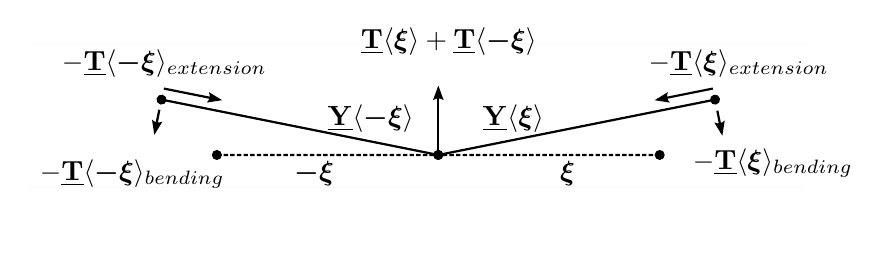
\begin{tikzpicture}[y=0.80pt, x=0.8pt,yscale=-1, inner sep=0pt, outer sep=0pt]
\begin{scope}[shift={(-16.10332,-55.70103)}]
  \begin{scope}[fill=black]
    \path[color=black,fill=black,line width=0.800pt] (101.0938,106.6875) --
      (103.0938,106.6875) -- (103.0938,105.6875) -- (101.0938,105.6875) --
      cycle(104.0938,106.6875) -- (106.0938,106.6875) -- (106.0938,105.6875) --
      (104.0938,105.6875) -- cycle(107.0938,106.6875) -- (109.0938,106.6875) --
      (109.0938,105.6875) -- (107.0938,105.6875) -- cycle(110.0938,106.6875) --
      (112.0938,106.6875) -- (112.0938,105.6875) -- (110.0938,105.6875) --
      cycle(113.0938,106.6875) -- (115.0938,106.6875) -- (115.0938,105.6875) --
      (113.0938,105.6875) -- cycle(116.0938,106.6875) -- (118.0938,106.6875) --
      (118.0938,105.6875) -- (116.0938,105.6875) -- cycle(119.0938,106.6875) --
      (121.0938,106.6875) -- (121.0938,105.6875) -- (119.0938,105.6875) --
      cycle(122.0938,106.6875) -- (124.0938,106.6875) -- (124.0938,105.6875) --
      (122.0938,105.6875) -- cycle(125.0938,106.6875) -- (127.0938,106.6875) --
      (127.0938,105.6875) -- (125.0938,105.6875) -- cycle(128.0938,106.6875) --
      (130.0938,106.6875) -- (130.0938,105.6875) -- (128.0938,105.6875) --
      cycle(131.0938,106.6875) -- (133.0938,106.6875) -- (133.0938,105.6875) --
      (131.0938,105.6875) -- cycle(134.0938,106.6875) -- (136.0938,106.6875) --
      (136.0938,105.6875) -- (134.0938,105.6875) -- cycle(137.0938,106.6875) --
      (139.0938,106.6875) -- (139.0938,105.6875) -- (137.0938,105.6875) --
      cycle(140.0938,106.6875) -- (142.0938,106.6875) -- (142.0938,105.6875) --
      (140.0938,105.6875) -- cycle(143.0938,106.6875) -- (145.0938,106.6875) --
      (145.0938,105.6875) -- (143.0938,105.6875) -- cycle(146.0938,106.6875) --
      (148.0938,106.6875) -- (148.0938,105.6875) -- (146.0938,105.6875) --
      cycle(149.0938,106.6875) -- (151.0938,106.6875) -- (151.0938,105.6875) --
      (149.0938,105.6875) -- cycle(152.0938,106.6875) -- (154.0938,106.6875) --
      (154.0938,105.6875) -- (152.0938,105.6875) -- cycle(155.0938,106.6875) --
      (157.0938,106.6875) -- (157.0938,105.6875) -- (155.0938,105.6875) --
      cycle(158.0938,106.6875) -- (160.0938,106.6875) -- (160.0938,105.6875) --
      (158.0938,105.6875) -- cycle(161.0938,106.6875) -- (163.0938,106.6875) --
      (163.0938,105.6875) -- (161.0938,105.6875) -- cycle(164.0938,106.6875) --
      (166.0938,106.6875) -- (166.0938,105.6875) -- (164.0938,105.6875) --
      cycle(167.0938,106.6875) -- (169.0938,106.6875) -- (169.0938,105.6875) --
      (167.0938,105.6875) -- cycle(170.0938,106.6875) -- (172.0938,106.6875) --
      (172.0938,105.6875) -- (170.0938,105.6875) -- cycle(173.0938,106.6875) --
      (175.0938,106.6875) -- (175.0938,105.6875) -- (173.0938,105.6875) --
      cycle(176.0938,106.6875) -- (178.0938,106.6875) -- (178.0938,105.6875) --
      (176.0938,105.6875) -- cycle(179.0938,106.6875) -- (181.0938,106.6875) --
      (181.0938,105.6875) -- (179.0938,105.6875) -- cycle(182.0938,106.6875) --
      (184.0938,106.6875) -- (184.0938,105.6875) -- (182.0938,105.6875) --
      cycle(185.0938,106.6875) -- (187.0938,106.6875) -- (187.0938,105.6875) --
      (185.0938,105.6875) -- cycle(188.0938,106.6875) -- (190.0938,106.6875) --
      (190.0938,105.6875) -- (188.0938,105.6875) -- cycle(191.0938,106.6875) --
      (193.0938,106.6875) -- (193.0938,105.6875) -- (191.0938,105.6875) --
      cycle(194.0938,106.6875) -- (196.0938,106.6875) -- (196.0938,105.6875) --
      (194.0938,105.6875) -- cycle(197.0938,106.6875) -- (199.0938,106.6875) --
      (199.0938,105.6875) -- (197.0938,105.6875) -- cycle(200.0938,106.6875) --
      (201.0938,106.6875) -- (202.0938,106.6875) -- (202.0938,105.6875) --
      (201.0938,105.6875) -- (200.0938,105.6875) -- cycle(203.0938,106.6875) --
      (205.0938,106.6875) -- (205.0938,105.6875) -- (203.0938,105.6875) --
      cycle(206.0938,106.6875) -- (208.0938,106.6875) -- (208.0938,105.6875) --
      (206.0938,105.6875) -- cycle(209.0938,106.6875) -- (211.0938,106.6875) --
      (211.0938,105.6875) -- (209.0938,105.6875) -- cycle(212.0938,106.6875) --
      (214.0938,106.6875) -- (214.0938,105.6875) -- (212.0938,105.6875) --
      cycle(215.0938,106.6875) -- (217.0938,106.6875) -- (217.0938,105.6875) --
      (215.0938,105.6875) -- cycle(218.0938,106.6875) -- (220.0938,106.6875) --
      (220.0938,105.6875) -- (218.0938,105.6875) -- cycle(221.0938,106.6875) --
      (223.0938,106.6875) -- (223.0938,105.6875) -- (221.0938,105.6875) --
      cycle(224.0938,106.6875) -- (226.0938,106.6875) -- (226.0938,105.6875) --
      (224.0938,105.6875) -- cycle(227.0938,106.6875) -- (229.0938,106.6875) --
      (229.0938,105.6875) -- (227.0938,105.6875) -- cycle(230.0938,106.6875) --
      (232.0938,106.6875) -- (232.0938,105.6875) -- (230.0938,105.6875) --
      cycle(233.0938,106.6875) -- (235.0938,106.6875) -- (235.0938,105.6875) --
      (233.0938,105.6875) -- cycle(236.0938,106.6875) -- (238.0938,106.6875) --
      (238.0938,105.6875) -- (236.0938,105.6875) -- cycle(239.0938,106.6875) --
      (241.0938,106.6875) -- (241.0938,105.6875) -- (239.0938,105.6875) --
      cycle(242.0938,106.6875) -- (244.0938,106.6875) -- (244.0938,105.6875) --
      (242.0938,105.6875) -- cycle(245.0938,106.6875) -- (247.0938,106.6875) --
      (247.0938,105.6875) -- (245.0938,105.6875) -- cycle(248.0938,106.6875) --
      (250.0938,106.6875) -- (250.0938,105.6875) -- (248.0938,105.6875) --
      cycle(251.0938,106.6875) -- (253.0938,106.6875) -- (253.0938,105.6875) --
      (251.0938,105.6875) -- cycle(254.0938,106.6875) -- (256.0938,106.6875) --
      (256.0938,105.6875) -- (254.0938,105.6875) -- cycle(257.0938,106.6875) --
      (259.0938,106.6875) -- (259.0938,105.6875) -- (257.0938,105.6875) --
      cycle(260.0938,106.6875) -- (262.0938,106.6875) -- (262.0938,105.6875) --
      (260.0938,105.6875) -- cycle(263.0938,106.6875) -- (265.0938,106.6875) --
      (265.0938,105.6875) -- (263.0938,105.6875) -- cycle(266.0938,106.6875) --
      (268.0938,106.6875) -- (268.0938,105.6875) -- (266.0938,105.6875) --
      cycle(269.0938,106.6875) -- (271.0938,106.6875) -- (271.0938,105.6875) --
      (269.0938,105.6875) -- cycle(272.0938,106.6875) -- (274.0938,106.6875) --
      (274.0938,105.6875) -- (272.0938,105.6875) -- cycle(275.0938,106.6875) --
      (277.0938,106.6875) -- (277.0938,105.6875) -- (275.0938,105.6875) --
      cycle(278.0938,106.6875) -- (280.0938,106.6875) -- (280.0938,105.6875) --
      (278.0938,105.6875) -- cycle(281.0938,106.6875) -- (283.0938,106.6875) --
      (283.0938,105.6875) -- (281.0938,105.6875) -- cycle(284.0938,106.6875) --
      (286.0938,106.6875) -- (286.0938,105.6875) -- (284.0938,105.6875) --
      cycle(287.0938,106.6875) -- (289.0938,106.6875) -- (289.0938,105.6875) --
      (287.0938,105.6875) -- cycle(290.0938,106.6875) -- (292.0938,106.6875) --
      (292.0938,105.6875) -- (290.0938,105.6875) -- cycle(293.0938,106.6875) --
      (295.0938,106.6875) -- (295.0938,105.6875) -- (293.0938,105.6875) --
      cycle(296.0938,106.6875) -- (298.0938,106.6875) -- (298.0938,105.6875) --
      (296.0938,105.6875) -- cycle(299.0938,106.6875) -- (301.0938,106.6875) --
      (301.0938,105.6875) -- (299.0938,105.6875) -- cycle;
    \path[draw=black,fill=black,even odd rule,line width=0.400pt]
      (103.0633,106.2010) .. controls (103.0633,107.3050) and (102.1673,108.2010) ..
      (101.0633,108.2010) .. controls (99.9593,108.2010) and (99.0633,107.3050) ..
      (99.0633,106.2010) .. controls (99.0633,105.0970) and (99.9593,104.2010) ..
      (101.0633,104.2010) .. controls (102.1673,104.2010) and (103.0633,105.0970) ..
      (103.0633,106.2010) -- cycle;
    \path[draw=black,fill=black,even odd rule,line width=0.400pt]
      (203.0633,106.2010) .. controls (203.0633,107.3050) and (202.1673,108.2010) ..
      (201.0633,108.2010) .. controls (199.9593,108.2010) and (199.0633,107.3050) ..
      (199.0633,106.2010) .. controls (199.0633,105.0970) and (199.9593,104.2010) ..
      (201.0633,104.2010) .. controls (202.1673,104.2010) and (203.0633,105.0970) ..
      (203.0633,106.2010) -- cycle;
    \path[draw=black,fill=black,even odd rule,line width=0.400pt]
      (303.0633,106.2010) .. controls (303.0633,107.3050) and (302.1673,108.2010) ..
      (301.0633,108.2010) .. controls (299.9593,108.2010) and (299.0633,107.3050) ..
      (299.0633,106.2010) .. controls (299.0633,105.0970) and (299.9593,104.2010) ..
      (301.0633,104.2010) .. controls (302.1673,104.2010) and (303.0633,105.0970) ..
      (303.0633,106.2010) -- cycle;
  \end{scope}
  \begin{scope}[fill=black]
    \path[color=black,fill=black,line width=0.800pt] (76.1875,80.7188) --
      (76.0000,81.6875) -- (201.0000,106.6875) -- (201.0937,106.7187) --
      (201.1874,106.6875) -- (326.1874,81.6875) -- (326.0000,80.7188) --
      (201.0938,105.6875) -- (76.1875,80.7188) -- cycle;
    \path[draw=black,fill=black,even odd rule,line width=0.400pt] (78.0253,81.5854)
      .. controls (77.8087,82.6680) and (76.7544,83.3709) .. (75.6719,83.1544) ..
      controls (74.5893,82.9378) and (73.8864,81.8835) .. (74.1029,80.8010) ..
      controls (74.3194,79.7184) and (75.3738,79.0155) .. (76.4563,79.2320) ..
      controls (77.5389,79.4485) and (78.2418,80.5029) .. (78.0253,81.5854) --
      cycle;
    \path[draw=black,fill=black,even odd rule,line width=0.400pt]
      (203.0633,106.2010) .. controls (203.0633,107.3050) and (202.1673,108.2010) ..
      (201.0633,108.2010) .. controls (199.9593,108.2010) and (199.0633,107.3050) ..
      (199.0633,106.2010) .. controls (199.0633,105.0970) and (199.9593,104.2010) ..
      (201.0633,104.2010) .. controls (202.1673,104.2010) and (203.0633,105.0970) ..
      (203.0633,106.2010) -- cycle;
    \path[draw=black,fill=black,even odd rule,line width=0.400pt] (328.0253,80.8166)
      .. controls (328.2418,81.8992) and (327.5389,82.9535) .. (326.4563,83.1700) ..
      controls (325.3738,83.3866) and (324.3194,82.6837) .. (324.1029,81.6011) ..
      controls (323.8864,80.5186) and (324.5893,79.4642) .. (325.6719,79.2477) ..
      controls (326.7544,79.0312) and (327.8087,79.7341) .. (328.0253,80.8166) --
      cycle;
  \end{scope}
  \begin{scope}[fill=black]
    \path[color=black,fill=black,line width=0.800pt] (200.5938,76.1875) --
      (200.5938,106.1875) -- (201.5938,106.1875) -- (201.5938,76.1875) --
      (200.5938,76.1875) -- cycle;
    \path[fill=black,line join=round,even odd rule,line width=0.500pt]
      (198.6831,81.4322) -- (201.0937,74.8767) -- (203.5043,81.4322) .. controls
      (202.0811,80.3849) and (200.1339,80.3909) .. (198.6831,81.4322) -- cycle;
  \end{scope}
  \path[fill=black] (178.797,148.02312) node[above right] (text6246) {};
  \path[fill=black] (256.10333,120.20103) node[above right] (text6273)
    {$\boldsymbol{\xi}$};
  \path[fill=black] (136.10332,120.20103) node[above right] (text6277)
    {$\boldsymbol{-\xi}$};
  \path[fill=black] (296.10333,71.201035) node[above right] (text6285)
    {$-\vstate{T}{}{\boldsymbol{\xi}}_{extension}$};
  \path[shift={(71.10332,65.91978)},draw=black,opacity=0.010,line join=miter,line
    cap=butt,line width=0.800pt] (-55.0000,54.7812) -- (295.0000,54.7812);
  \path[fill=black] (316.10333,116.20103) node[above right] (text4473)
    {$-\vstate{T}{}{\boldsymbol{\xi}}_{bending}$};
  \begin{scope}[shift={(0,-64.5)},shift={(0,0)}]
    \path[shift={(71.10332,65.91978)},draw=black,opacity=0.010,line join=miter,line
      cap=butt,line width=0.800pt] (-55.0000,54.7812) -- (295.0000,54.7812);
  \end{scope}
  \path[fill=black] (166.10332,61.201035) node[above right] (text4726)
    {$\vstate{T}{}{\boldsymbol{\xi}}+\vstate{T}{}{\boldsymbol{-\xi}}$};
  \begin{scope}[fill=black]
    \path[color=black,fill=black,line width=0.800pt] (74.5625,85.6875) --
      (72.5625,95.6875) -- (73.5625,95.9062) -- (75.5625,85.9062) --
      (74.5625,85.6875) -- cycle;
    \path[fill=black,line join=round,even odd rule,line width=0.500pt]
      (76.4671,91.1458) -- (72.8177,97.1013) -- (71.7395,90.2003) .. controls
      (72.9297,91.5064) and (74.8403,91.8824) .. (76.4671,91.1458) -- cycle;
  \end{scope}
  \begin{scope}[fill=black]
    \path[color=black,fill=black,line width=0.800pt] (77.1875,75.7188) --
      (77.0000,76.6875) -- (102.0000,81.6875) -- (102.1875,80.7188) --
      (77.1875,75.7188) -- cycle;
    \path[fill=black,line join=round,even odd rule,line width=0.500pt]
      (97.4484,77.8019) -- (103.4039,81.4513) -- (96.5029,82.5295) .. controls
      (97.8090,81.3393) and (98.1849,79.4287) .. (97.4484,77.8019) -- cycle;
  \end{scope}
  \begin{scope}[fill=black]
    \path[color=black,fill=black,line width=0.800pt] (327.5938,86.0938) --
      (326.6250,86.3125) -- (328.6250,96.3125) -- (329.5938,96.0938) --
      (327.5938,86.0938) -- cycle;
    \path[fill=black,line join=round,even odd rule,line width=0.500pt]
      (330.4506,90.5968) -- (329.3725,97.4978) -- (325.7230,91.5423) .. controls
      (327.3240,92.2902) and (329.2322,91.9024) .. (330.4507,90.5968) -- cycle;
  \end{scope}
  \begin{scope}[fill=black]
    \path[color=black,fill=black,line width=0.800pt] (325.0000,75.7188) --
      (300.0000,80.7188) -- (300.1875,81.6875) -- (325.1875,76.6875) --
      (325.0000,75.7188) -- cycle;
    \path[fill=black,line join=round,even odd rule,line width=0.500pt]
      (305.7075,82.5484) -- (298.8066,81.4702) -- (304.7620,77.8207) .. controls
      (304.0142,79.4217) and (304.4020,81.3299) .. (305.7075,82.5484) -- cycle;
  \end{scope}
  \path[fill=black] (21.103317,121.20103) node[above right] (text4217)
    {$-\vstate{T}{}{\boldsymbol{-\xi}}_{bending}$};
  \path[fill=black] (31.103317,71.201035) node[above right] (text4221)
    {$-\vstate{T}{}{\boldsymbol{-\xi}}_{extension}$};
  \path[fill=black] (221.10332,96.201035) node[above right] (text4282)
    {$\vstate{Y}{}{\boldsymbol{\xi}}$};
  \path[fill=black] (151.10332,96.201035) node[above right] (text4286)
    {$\vstate{Y}{}{\boldsymbol{-\xi}}$};
\end{scope}

\end{tikzpicture}


  \caption{The Hybrid Model Combines Bending and Extension Components}
  \label{fig:hybridmodel}
\end{figure}
%
As the two sides are pulled apart, the magnitude of the extension force in each bond increases, and the magnitude of the bending force decreases.  At the same time, the angle at which the extension force acts decreases, and the angle of action for the bending force increases.  For small amounts of bending and reasonable stretches, increased tension in the direction of the bond pair results in increase restorative force.

\section{Extension to arbitrary Poisson ratio}
\label{sec:arbitrary}
Although many materials have Poisson ratios of \(\nu\approx \sfrac{1}{3}\), it is nonetheless desirable to extend the model to materials with arbitrary Poisson ratios.  For isotropic, linearly elastic models of solid materials, Silling et al.\ extended the peridynamic material model to arbitrary material parameters in \cite{silling2007peridynamic} by decomposing the deformation into isotropic and deviatoric components.  In the absence of plastic deformation, we need only find the difference between the strain energy of a deformed bond-based plate and the strain energy of an elastic plate with Poisson's ratio \(\nu \neq \sfrac{1}{3}\).  The difference is a function of the isotropic strain in two dimensions, \(\theta_2\)
%
\begin{align}
    W' &= \frac{G\;h}{2}\left(\frac{3\nu-1}{1-\nu}\right)\theta_2^2 \notag \\
%    \theta_2 &= \frac{2}{m}\left(\underline{\omega x}\right)\bullet\underline{e} \notag \\
    \theta_2 &= \frac{2}{m}\int_A \omega(\boldsymbol{\xi})|\boldsymbol{\xi}|(|\vstate{Y}{}{\boldsymbol{\xi}}|-|\boldsymbol{\xi}|)\;dA_{\boldsymbol{\xi}} \notag \\
%    W_\text{total} &= \frac{G\;h}{2}\left(\frac{3\nu-1}{1-\nu}\right)\theta_2^2 + \frac{4\;G\;h}{m}\left(\underline{\omega e}\right)\bullet\underline{e}\notag
    W_\text{total} &= \frac{G\;h}{2}\left(\frac{3\nu-1}{1-\nu}\right)\theta_2^2 + \frac{4\;G\;h}{m}\int_A \omega(\boldsymbol{\xi})(|\vstate{Y}{}{\boldsymbol{\xi}}|-|\boldsymbol{\xi}|)^2\;dA_{\boldsymbol{\xi}}\notag
\end{align}
%
This is to be expected because the bond-based model was calibrated to the shear strain energy, leaving discrepancies proportional to the isotropic strain energy that fall to 0 as Poisson's ratio approaches \(\nu = \sfrac{1}{3}\).

This decomposition method inspires a similar approach to our plate model. To perform the same extension for the plate model in bending, we find the error in the 1-parameter strain energy for \(\nu \neq \sfrac{1}{3}\)
%
\begin{align}
    W'=&\frac{G h^3}{12(1-\nu)} \left(\kappa_1^2+\kappa_2^2+2\nu\kappa_1\kappa_2+2(1-\nu)\kappa_3^2 \right)\notag\\
    &-\frac{G h^3}{12(1-\frac{1}{3})} \left(\kappa_1^2+\kappa_2^2+\frac{2}{3}\nu\kappa_1\kappa_2+2(1-\frac{1}{3})\kappa_3^2 \right) \notag \\
    W'=&2G \frac{h^3}{12}\frac{3\nu-1}{1-\nu} \left(\frac{\kappa_1+\kappa_2}{2}\right)^2.\notag
\end{align}
%
The discrepancy in energy is proportional to the square of average curvature, \(\frac{\kappa_1+\kappa_2}{2} = \bar{\kappa}\), which we will also refer to as the isotropic curvature.  The isotropic curvature can be envisioned as the portion of the deformation that resembles a hemispherical bowl.  A complete decomposition of bending energy into isotropic and deviatoric components as performed by Fischer in \cite{fischer1992bending} produces a far more complex model and is unnecessary at this time.  For a single bond pair we can represent the curvature vector along the bond pair as 
%\marginpar{ maybe leave this out and go straight to the curvature vector?}
%
\begin{equation}
    \boldsymbol{\kappa} _{\hat{\boldsymbol{\xi}}} = \frac{\vstate{Y}{}{\boldsymbol{\xi}}+\vstate{Y}{}{\boldsymbol{-\xi}}}{|\boldsymbol{\xi}|^2}\notag
\end{equation}
%
%\begin{equation}
%    \kappa_{\hat{u}} = \frac{z(\mathbf{x}+\xi\hat{u})-2z(\mathbf{x})+z(\mathbf{x}-\xi\hat{u})}{\xi^2}\notag
%\end{equation}
%
For large rotations, we can define an average curvature vector \(\bar{\boldsymbol{\kappa}}\).
This leads us to model the average curvature as 
%
\begin{align}
    \bar{\boldsymbol{\kappa}} &= \frac{1}{m} \int_0^\delta \int_0^{2\pi}\omega(\xi)\frac{\vstate{Y}{}{\boldsymbol{\xi}}+\vstate{Y}{}{\boldsymbol{-\xi}}}{\xi^2} \xi {\rm d}\phi {\rm d}\xi ;\notag \\
    m &= \int_0^\delta \int_0^{2\pi}\omega(\xi)\xi {\rm d}\phi {\rm d}\xi. \notag
\end{align}
%
The weighting function \(\omega(\xi)\) performs the same function as in the previous section.
We can rewrite the energy discrepancy in terms of \(\bar{\boldsymbol{\kappa}}\).
%
\begin{equation}
    W'=2G\frac{h^3}{12}\frac{3\nu-1}{1-\nu}\bar{\boldsymbol{\kappa}}^2. \notag
\end{equation}
%
We can take the Fr\'{e}chet derivative (details in \ref{sec:frechet})\todo{Can you show the details in the Appendix?  Also, should the $dA$ be there?} to produce a correction force vector state
%
\begin{equation}
    \vstate{T'}{}{\boldsymbol{\xi}}=\frac{8G}{m}\frac{h^3}{12}\frac{3\nu-1}{1-\nu}\frac{\omega(\boldsymbol{\xi})}{\xi^2} \bar{\boldsymbol{\kappa}},
    \label{eq:pressureState}
\end{equation}
%
that is not directly dependent on the deformation of a single bond pair.  Instead, \cref{eq:pressureState} represents a bond-length dependent ``pressure'' applied to every pair of bonds extending from a node.  This ``pressure'' is proportional to the curvature vector at that node.
A weighting function \(\omega(\boldsymbol{\xi}) = |\boldsymbol{\xi}|\) can ensure that the integral expression for force at a point is convergent.  This extra term that is dependent on the bending of all the pairs around a material point means that the extension is not properly a \textit{bond-pair} model.  Instead, it would be more accurate to call it a \textit{bond-multiple} model, in which the bond forces and energies are functions of the relationship between a family of bonds.  In either the continuous or discrete cases, this model extension requires the additional step of evaluating the isotropic curvature at each point, but the increased complexity of the extended model captures in the local limit the behavior of a two-parameter elastic material plate.
%
\section{Numerical Simulation}
\subsection{Discretized Model}
Discretizing the bond-pair model is primarily matter of exchanging integrals for sums. 
%
\begin{align}
%\label{eq:discreteBeamw}
w(\boldsymbol{\xi}_i) &= \omega(\boldsymbol{\xi}_i)\alpha \left[1+\cos(\theta(\vstate{Y}{}{\boldsymbol{\xi}_i},\vstate{Y}{}{-\boldsymbol{\xi}_i})) \right] \notag \\
&\approx \omega(\boldsymbol{\xi}_i)\frac{\alpha}{2}\left(\frac{z(\mathbf{x}+\boldsymbol{\xi}_i)-2z(\mathbf{x})+z(\mathbf{x}-\boldsymbol{\xi}_i)}{\boldsymbol{\xi}_i}\right)^2 \notag
\end{align}
%
in which $\boldsymbol{\xi}_i$ is the $i^\textnormal{th}$ bond emanating from the point $\mathbf{x}$ to each of the $n$ points within distance $\delta$ of point $\mathbf{x}$.
%
\begin{align}
%    \label{eq:discretebeam}
    \alpha &= \frac{c\; (\Delta x)^2}{m} ;\; c= \frac{G}{(1-\nu)}\frac{h^3}{12};\; m=\sum_{i=1}^n \omega(\boldsymbol{\xi}_i)\boldsymbol{\xi}_i^2 \implies \nonumber \\
    W&=(\Delta x)^2 \sum_{i=1}^n \omega(\boldsymbol{\xi}_i)\frac{G}{2(1-\nu)}\frac{h^3}{12}\left(\frac{z(\mathbf{x}+\boldsymbol{\xi}_i)-2z(\mathbf{x})+z(\mathbf{x}-\boldsymbol{\xi}_i)}{|\boldsymbol{\xi}_i|}\right)^2 \notag
\end{align}
%
Discretization of the 1-parameter bending model results in the equation of motion
%
\begin{align}
    \label{eq:discreteEoM}
    \rho(\mathbf{x})\mathbf{\ddot{u}}(\mathbf{x}) = \mathbf{f}(\mathbf{x})&+\sum_i \omega(\boldsymbol{\xi}_i)\left\{\frac{\alpha(\mathbf{x})}{|\mathbf{p}_i |}\frac{\mathbf{p}_i}{|\mathbf{p}_i |}\times \left[ \frac{\mathbf{p}_i}{|\mathbf{p}_i |}\times \frac{\mathbf{q}_i}{|\mathbf{q}_i |}\right] \right.  \\
    & \left. -\frac{\alpha(\mathbf{x}+\boldsymbol{\xi}_i)}{|\mathbf{p}_i |}\frac{(-\mathbf{p}_i)}{|\mathbf{p}_i |}\times\left[\frac{(-\mathbf{p}_i)}{|\mathbf{p}_i |}\times \frac{\mathbf{r}_i}{|\mathbf{r}_i |} \right] \right\} \notag
\end{align}
with
\begin{align}
    \mathbf{p}_i &= \boldsymbol{\xi}_i+\mathbf{u}(\mathbf{x}+\boldsymbol{\xi}_i)-\mathbf{u}(\mathbf{x});\notag\\
    \mathbf{q}_i &= -\boldsymbol{\xi}_i+\mathbf{u}(\mathbf{x}-\boldsymbol{\xi}_i)-\mathbf{u}(\mathbf{x});\notag\\
    \mathbf{r}_i &= \boldsymbol{\xi}_i+\mathbf{u}(\mathbf{x}+2\boldsymbol{\xi}_i)-\mathbf{u}(\mathbf{x}+\boldsymbol{\xi}_i).\notag
\end{align}
%

Implementing the 2-parameter model requires finding the isotropic curvature at each point.
%
\begin{align*}
    \bar{\boldsymbol{\kappa}}(\mathbf{x}) &= \frac{1}{m} \sum_i \omega(\boldsymbol{\xi}_i)\frac{\mathbf{p}_i +\mathbf{q}_i }{\boldsymbol{\xi}_i^2};\notag \\
    m(\mathbf{x})  &= \sum_i \omega(\boldsymbol{\xi}_i); \notag \\
    \alpha^\text{iso}(\mathbf{x}) &= \frac{4G}{m}\frac{h^3}{12}\frac{3\nu-1}{1-\nu}(\Delta x)^2;\\
    f^\text{iso}(\mathbf{x}) &= \sum_j \left\{\left[\alpha^\text{iso}(\mathbf{x})\bar{\boldsymbol{\kappa}}(\mathbf{x})-\alpha^\text{iso}(\mathbf{x}+\boldsymbol{\xi}_j)\bar{\boldsymbol{\kappa}}(\mathbf{x}+\boldsymbol{\xi}_j) \right] \frac{\omega(\boldsymbol{\xi}_j)}{\boldsymbol{\xi}_j^2} \right\}
\end{align*}
%
Discretizing the bond-pair model as proposed above requires that nodes be evenly spaced, $\Delta x$, throughout the entire plate, otherwise the displacement \(z(\mathbf{x}-\boldsymbol{\xi}_i)\) is ill-defined.  For this reason, the discretization does not allow for areas of higher and lower ``resolution''. An extension to this discretization that would allow changing mesh resolution will require interpolation between the nodes.  
%
\subsection{Numerical Method}
\label{sec:NumMethod}
Model behavior is evaluated by implementing the discretized equation of motion.  The case of a square plate simply supported on all four sides is chosen for simplicity in both evaluation and comparison.  To implement the simply-supported condition, it was sufficient to constrain the vertical displacement of each node along the plate's four edges.  Boundary conditions such as clamped or guided supports and applied moments require careful treatment to ensure both meaningful results and ease of computation.  While applying displacement constraints is straightforward, the appropriate way to apply an angle constraint or moment to a peridynamic point or collection of points is less obvious.

Additionally, the simply-supported flat plate is a configuration with significant analytical treatment in the classical theories, making a better comparison case than configurations that may require comparison to finite element or other solution techniques.
%
\subsection{Results}
The simplest test case for this model is a linear-elastic square plate with Poisson's ratio \(\nu = \sfrac{1}{3}\) that is simply-supported on all 4 sides with a uniform transverse pressure load on the entire surface between the supports.  As expected from an energy-equivalent model, the slice along the plate's centerline shown in \cref{fig:plate_convergence_h} demonstrates good agreement between the static deflection predicted by the bond-pair model and that of classical linear elasticity as the horizon length shrinks.  This convergence only continues to a minimum horizon, below which the discretized equation of motion (\cref{eq:discreteEoM}) ceases to accurately approximate the continuous integral formulation (\cref{eq:PDstateEoM,eq:SillingForceNO}).  The minimum horizon size depends on the discretization; it appears that twice the node spacing is insufficient, and that three times the node spacing is sufficient.  The difference is evident in \cref{fig:plate_minimum_h}.
%
\begin{figure}[h]
  \centering
  \resizebox{0.55\linewidth}{!}{%% Creator: Matplotlib, PGF backend
%%
%% To include the figure in your LaTeX document, write
%%   \input{<filename>.pgf}
%%
%% Make sure the required packages are loaded in your preamble
%%   \usepackage{pgf}
%%
%% Figures using additional raster images can only be included by \input if
%% they are in the same directory as the main LaTeX file. For loading figures
%% from other directories you can use the `import` package
%%   \usepackage{import}
%% and then include the figures with
%%   \import{<path to file>}{<filename>.pgf}
%%
%% Matplotlib used the following preamble
%%
\begingroup%
\makeatletter%
\begin{pgfpicture}%
\pgfpathrectangle{\pgfpointorigin}{\pgfqpoint{6.000000in}{6.000000in}}%
\pgfusepath{use as bounding box}%
\begin{pgfscope}%
\pgfsetrectcap%
\pgfsetroundjoin%
\definecolor{currentfill}{rgb}{1.000000,1.000000,1.000000}%
\pgfsetfillcolor{currentfill}%
\pgfsetlinewidth{0.000000pt}%
\definecolor{currentstroke}{rgb}{1.000000,1.000000,1.000000}%
\pgfsetstrokecolor{currentstroke}%
\pgfsetdash{}{0pt}%
\pgfpathmoveto{\pgfqpoint{0.000000in}{0.000000in}}%
\pgfpathlineto{\pgfqpoint{6.000000in}{0.000000in}}%
\pgfpathlineto{\pgfqpoint{6.000000in}{6.000000in}}%
\pgfpathlineto{\pgfqpoint{0.000000in}{6.000000in}}%
\pgfpathclose%
\pgfusepath{fill}%
\end{pgfscope}%
\begin{pgfscope}%
\pgfsetrectcap%
\pgfsetroundjoin%
\definecolor{currentfill}{rgb}{1.000000,1.000000,1.000000}%
\pgfsetfillcolor{currentfill}%
\pgfsetlinewidth{0.000000pt}%
\definecolor{currentstroke}{rgb}{0.000000,0.000000,0.000000}%
\pgfsetstrokecolor{currentstroke}%
\pgfsetdash{}{0pt}%
\pgfpathmoveto{\pgfqpoint{0.750000in}{0.600000in}}%
\pgfpathlineto{\pgfqpoint{5.400000in}{0.600000in}}%
\pgfpathlineto{\pgfqpoint{5.400000in}{5.400000in}}%
\pgfpathlineto{\pgfqpoint{0.750000in}{5.400000in}}%
\pgfpathclose%
\pgfusepath{fill}%
\end{pgfscope}%
\begin{pgfscope}%
\pgfpathrectangle{\pgfqpoint{0.750000in}{0.600000in}}{\pgfqpoint{4.650000in}{4.800000in}} %
\pgfusepath{clip}%
\pgfsetrectcap%
\pgfsetroundjoin%
\pgfsetlinewidth{1.003750pt}%
\definecolor{currentstroke}{rgb}{0.000000,0.000000,1.000000}%
\pgfsetstrokecolor{currentstroke}%
\pgfsetdash{}{0pt}%
\pgfpathmoveto{\pgfqpoint{0.750000in}{5.400000in}}%
\pgfpathlineto{\pgfqpoint{0.796500in}{5.270617in}}%
\pgfpathlineto{\pgfqpoint{0.843000in}{5.141433in}}%
\pgfpathlineto{\pgfqpoint{0.889500in}{5.012646in}}%
\pgfpathlineto{\pgfqpoint{0.936000in}{4.884446in}}%
\pgfpathlineto{\pgfqpoint{0.982500in}{4.757015in}}%
\pgfpathlineto{\pgfqpoint{1.029000in}{4.630524in}}%
\pgfpathlineto{\pgfqpoint{1.075500in}{4.505137in}}%
\pgfpathlineto{\pgfqpoint{1.122000in}{4.381006in}}%
\pgfpathlineto{\pgfqpoint{1.168500in}{4.258277in}}%
\pgfpathlineto{\pgfqpoint{1.215000in}{4.137087in}}%
\pgfpathlineto{\pgfqpoint{1.261500in}{4.017568in}}%
\pgfpathlineto{\pgfqpoint{1.308000in}{3.899846in}}%
\pgfpathlineto{\pgfqpoint{1.354500in}{3.784039in}}%
\pgfpathlineto{\pgfqpoint{1.401000in}{3.670263in}}%
\pgfpathlineto{\pgfqpoint{1.447500in}{3.558623in}}%
\pgfpathlineto{\pgfqpoint{1.494000in}{3.449222in}}%
\pgfpathlineto{\pgfqpoint{1.540500in}{3.342155in}}%
\pgfpathlineto{\pgfqpoint{1.587000in}{3.237511in}}%
\pgfpathlineto{\pgfqpoint{1.633500in}{3.135374in}}%
\pgfpathlineto{\pgfqpoint{1.680000in}{3.035823in}}%
\pgfpathlineto{\pgfqpoint{1.726500in}{2.938933in}}%
\pgfpathlineto{\pgfqpoint{1.773000in}{2.844775in}}%
\pgfpathlineto{\pgfqpoint{1.819500in}{2.753417in}}%
\pgfpathlineto{\pgfqpoint{1.866000in}{2.664922in}}%
\pgfpathlineto{\pgfqpoint{1.912500in}{2.579349in}}%
\pgfpathlineto{\pgfqpoint{1.959000in}{2.496753in}}%
\pgfpathlineto{\pgfqpoint{2.005500in}{2.417186in}}%
\pgfpathlineto{\pgfqpoint{2.052000in}{2.340695in}}%
\pgfpathlineto{\pgfqpoint{2.098500in}{2.267325in}}%
\pgfpathlineto{\pgfqpoint{2.145000in}{2.197118in}}%
\pgfpathlineto{\pgfqpoint{2.191500in}{2.130112in}}%
\pgfpathlineto{\pgfqpoint{2.238000in}{2.066343in}}%
\pgfpathlineto{\pgfqpoint{2.284500in}{2.005847in}}%
\pgfpathlineto{\pgfqpoint{2.331000in}{1.948654in}}%
\pgfpathlineto{\pgfqpoint{2.377500in}{1.894795in}}%
\pgfpathlineto{\pgfqpoint{2.424000in}{1.844294in}}%
\pgfpathlineto{\pgfqpoint{2.470500in}{1.797178in}}%
\pgfpathlineto{\pgfqpoint{2.517000in}{1.753468in}}%
\pgfpathlineto{\pgfqpoint{2.563500in}{1.713182in}}%
\pgfpathlineto{\pgfqpoint{2.610000in}{1.676341in}}%
\pgfpathlineto{\pgfqpoint{2.656500in}{1.642959in}}%
\pgfpathlineto{\pgfqpoint{2.703000in}{1.613052in}}%
\pgfpathlineto{\pgfqpoint{2.749500in}{1.586634in}}%
\pgfpathlineto{\pgfqpoint{2.796000in}{1.563715in}}%
\pgfpathlineto{\pgfqpoint{2.842500in}{1.544306in}}%
\pgfpathlineto{\pgfqpoint{2.889000in}{1.528416in}}%
\pgfpathlineto{\pgfqpoint{2.935500in}{1.516051in}}%
\pgfpathlineto{\pgfqpoint{2.982000in}{1.507215in}}%
\pgfpathlineto{\pgfqpoint{3.028500in}{1.501913in}}%
\pgfpathlineto{\pgfqpoint{3.075000in}{1.500145in}}%
\pgfpathlineto{\pgfqpoint{3.121500in}{1.501913in}}%
\pgfpathlineto{\pgfqpoint{3.168000in}{1.507215in}}%
\pgfpathlineto{\pgfqpoint{3.214500in}{1.516051in}}%
\pgfpathlineto{\pgfqpoint{3.261000in}{1.528416in}}%
\pgfpathlineto{\pgfqpoint{3.307500in}{1.544306in}}%
\pgfpathlineto{\pgfqpoint{3.354000in}{1.563715in}}%
\pgfpathlineto{\pgfqpoint{3.400500in}{1.586634in}}%
\pgfpathlineto{\pgfqpoint{3.447000in}{1.613052in}}%
\pgfpathlineto{\pgfqpoint{3.493500in}{1.642959in}}%
\pgfpathlineto{\pgfqpoint{3.540000in}{1.676341in}}%
\pgfpathlineto{\pgfqpoint{3.586500in}{1.713182in}}%
\pgfpathlineto{\pgfqpoint{3.633000in}{1.753468in}}%
\pgfpathlineto{\pgfqpoint{3.679500in}{1.797178in}}%
\pgfpathlineto{\pgfqpoint{3.726000in}{1.844294in}}%
\pgfpathlineto{\pgfqpoint{3.772500in}{1.894795in}}%
\pgfpathlineto{\pgfqpoint{3.819000in}{1.948654in}}%
\pgfpathlineto{\pgfqpoint{3.865500in}{2.005847in}}%
\pgfpathlineto{\pgfqpoint{3.912000in}{2.066343in}}%
\pgfpathlineto{\pgfqpoint{3.958500in}{2.130112in}}%
\pgfpathlineto{\pgfqpoint{4.005000in}{2.197118in}}%
\pgfpathlineto{\pgfqpoint{4.051500in}{2.267325in}}%
\pgfpathlineto{\pgfqpoint{4.098000in}{2.340695in}}%
\pgfpathlineto{\pgfqpoint{4.144500in}{2.417186in}}%
\pgfpathlineto{\pgfqpoint{4.191000in}{2.496753in}}%
\pgfpathlineto{\pgfqpoint{4.237500in}{2.579349in}}%
\pgfpathlineto{\pgfqpoint{4.284000in}{2.664922in}}%
\pgfpathlineto{\pgfqpoint{4.330500in}{2.753417in}}%
\pgfpathlineto{\pgfqpoint{4.377000in}{2.844775in}}%
\pgfpathlineto{\pgfqpoint{4.423500in}{2.938933in}}%
\pgfpathlineto{\pgfqpoint{4.470000in}{3.035823in}}%
\pgfpathlineto{\pgfqpoint{4.516500in}{3.135374in}}%
\pgfpathlineto{\pgfqpoint{4.563000in}{3.237511in}}%
\pgfpathlineto{\pgfqpoint{4.609500in}{3.342155in}}%
\pgfpathlineto{\pgfqpoint{4.656000in}{3.449222in}}%
\pgfpathlineto{\pgfqpoint{4.702500in}{3.558623in}}%
\pgfpathlineto{\pgfqpoint{4.749000in}{3.670263in}}%
\pgfpathlineto{\pgfqpoint{4.795500in}{3.784039in}}%
\pgfpathlineto{\pgfqpoint{4.842000in}{3.899846in}}%
\pgfpathlineto{\pgfqpoint{4.888500in}{4.017568in}}%
\pgfpathlineto{\pgfqpoint{4.935000in}{4.137087in}}%
\pgfpathlineto{\pgfqpoint{4.981500in}{4.258277in}}%
\pgfpathlineto{\pgfqpoint{5.028000in}{4.381006in}}%
\pgfpathlineto{\pgfqpoint{5.074500in}{4.505137in}}%
\pgfpathlineto{\pgfqpoint{5.121000in}{4.630524in}}%
\pgfpathlineto{\pgfqpoint{5.167500in}{4.757015in}}%
\pgfpathlineto{\pgfqpoint{5.214000in}{4.884446in}}%
\pgfpathlineto{\pgfqpoint{5.260500in}{5.012646in}}%
\pgfpathlineto{\pgfqpoint{5.307000in}{5.141433in}}%
\pgfpathlineto{\pgfqpoint{5.353500in}{5.270617in}}%
\pgfpathlineto{\pgfqpoint{5.400000in}{5.400000in}}%
\pgfusepath{stroke}%
\end{pgfscope}%
\begin{pgfscope}%
\pgfpathrectangle{\pgfqpoint{0.750000in}{0.600000in}}{\pgfqpoint{4.650000in}{4.800000in}} %
\pgfusepath{clip}%
\pgfsetbuttcap%
\pgfsetmiterjoin%
\definecolor{currentfill}{rgb}{0.000000,0.500000,0.000000}%
\pgfsetfillcolor{currentfill}%
\pgfsetlinewidth{0.501875pt}%
\definecolor{currentstroke}{rgb}{0.000000,0.000000,0.000000}%
\pgfsetstrokecolor{currentstroke}%
\pgfsetdash{}{0pt}%
\pgfsys@defobject{currentmarker}{\pgfqpoint{-0.041667in}{-0.041667in}}{\pgfqpoint{0.041667in}{0.041667in}}{%
\pgfpathmoveto{\pgfqpoint{0.000000in}{0.041667in}}%
\pgfpathlineto{\pgfqpoint{-0.041667in}{-0.041667in}}%
\pgfpathlineto{\pgfqpoint{0.041667in}{-0.041667in}}%
\pgfpathclose%
\pgfusepath{stroke,fill}%
}%
\begin{pgfscope}%
\pgfsys@transformshift{0.750000in}{5.400000in}%
\pgfsys@useobject{currentmarker}{}%
\end{pgfscope}%
\begin{pgfscope}%
\pgfsys@transformshift{1.029000in}{4.310547in}%
\pgfsys@useobject{currentmarker}{}%
\end{pgfscope}%
\begin{pgfscope}%
\pgfsys@transformshift{1.308000in}{3.564782in}%
\pgfsys@useobject{currentmarker}{}%
\end{pgfscope}%
\begin{pgfscope}%
\pgfsys@transformshift{1.587000in}{2.898760in}%
\pgfsys@useobject{currentmarker}{}%
\end{pgfscope}%
\begin{pgfscope}%
\pgfsys@transformshift{1.866000in}{2.327648in}%
\pgfsys@useobject{currentmarker}{}%
\end{pgfscope}%
\begin{pgfscope}%
\pgfsys@transformshift{2.145000in}{1.860336in}%
\pgfsys@useobject{currentmarker}{}%
\end{pgfscope}%
\begin{pgfscope}%
\pgfsys@transformshift{2.424000in}{1.508532in}%
\pgfsys@useobject{currentmarker}{}%
\end{pgfscope}%
\begin{pgfscope}%
\pgfsys@transformshift{2.703000in}{1.277825in}%
\pgfsys@useobject{currentmarker}{}%
\end{pgfscope}%
\begin{pgfscope}%
\pgfsys@transformshift{2.982000in}{1.172269in}%
\pgfsys@useobject{currentmarker}{}%
\end{pgfscope}%
\begin{pgfscope}%
\pgfsys@transformshift{3.261000in}{1.193421in}%
\pgfsys@useobject{currentmarker}{}%
\end{pgfscope}%
\begin{pgfscope}%
\pgfsys@transformshift{3.540000in}{1.340945in}%
\pgfsys@useobject{currentmarker}{}%
\end{pgfscope}%
\begin{pgfscope}%
\pgfsys@transformshift{3.819000in}{1.612666in}%
\pgfsys@useobject{currentmarker}{}%
\end{pgfscope}%
\begin{pgfscope}%
\pgfsys@transformshift{4.098000in}{2.002922in}%
\pgfsys@useobject{currentmarker}{}%
\end{pgfscope}%
\begin{pgfscope}%
\pgfsys@transformshift{4.377000in}{2.507482in}%
\pgfsys@useobject{currentmarker}{}%
\end{pgfscope}%
\begin{pgfscope}%
\pgfsys@transformshift{4.656000in}{3.109556in}%
\pgfsys@useobject{currentmarker}{}%
\end{pgfscope}%
\begin{pgfscope}%
\pgfsys@transformshift{4.935000in}{3.805866in}%
\pgfsys@useobject{currentmarker}{}%
\end{pgfscope}%
\begin{pgfscope}%
\pgfsys@transformshift{5.214000in}{4.578216in}%
\pgfsys@useobject{currentmarker}{}%
\end{pgfscope}%
\end{pgfscope}%
\begin{pgfscope}%
\pgfpathrectangle{\pgfqpoint{0.750000in}{0.600000in}}{\pgfqpoint{4.650000in}{4.800000in}} %
\pgfusepath{clip}%
\pgfsetbuttcap%
\pgfsetmiterjoin%
\definecolor{currentfill}{rgb}{1.000000,0.000000,0.000000}%
\pgfsetfillcolor{currentfill}%
\pgfsetlinewidth{0.501875pt}%
\definecolor{currentstroke}{rgb}{0.000000,0.000000,0.000000}%
\pgfsetstrokecolor{currentstroke}%
\pgfsetdash{}{0pt}%
\pgfsys@defobject{currentmarker}{\pgfqpoint{-0.041667in}{-0.041667in}}{\pgfqpoint{0.041667in}{0.041667in}}{%
\pgfpathmoveto{\pgfqpoint{-0.041667in}{-0.041667in}}%
\pgfpathlineto{\pgfqpoint{0.041667in}{-0.041667in}}%
\pgfpathlineto{\pgfqpoint{0.041667in}{0.041667in}}%
\pgfpathlineto{\pgfqpoint{-0.041667in}{0.041667in}}%
\pgfpathclose%
\pgfusepath{stroke,fill}%
}%
\begin{pgfscope}%
\pgfsys@transformshift{0.843000in}{5.061173in}%
\pgfsys@useobject{currentmarker}{}%
\end{pgfscope}%
\begin{pgfscope}%
\pgfsys@transformshift{1.122000in}{4.266410in}%
\pgfsys@useobject{currentmarker}{}%
\end{pgfscope}%
\begin{pgfscope}%
\pgfsys@transformshift{1.401000in}{3.542014in}%
\pgfsys@useobject{currentmarker}{}%
\end{pgfscope}%
\begin{pgfscope}%
\pgfsys@transformshift{1.680000in}{2.900482in}%
\pgfsys@useobject{currentmarker}{}%
\end{pgfscope}%
\begin{pgfscope}%
\pgfsys@transformshift{1.959000in}{2.358675in}%
\pgfsys@useobject{currentmarker}{}%
\end{pgfscope}%
\begin{pgfscope}%
\pgfsys@transformshift{2.238000in}{1.927894in}%
\pgfsys@useobject{currentmarker}{}%
\end{pgfscope}%
\begin{pgfscope}%
\pgfsys@transformshift{2.517000in}{1.615664in}%
\pgfsys@useobject{currentmarker}{}%
\end{pgfscope}%
\begin{pgfscope}%
\pgfsys@transformshift{2.796000in}{1.426642in}%
\pgfsys@useobject{currentmarker}{}%
\end{pgfscope}%
\begin{pgfscope}%
\pgfsys@transformshift{3.075000in}{1.363366in}%
\pgfsys@useobject{currentmarker}{}%
\end{pgfscope}%
\begin{pgfscope}%
\pgfsys@transformshift{3.354000in}{1.426642in}%
\pgfsys@useobject{currentmarker}{}%
\end{pgfscope}%
\begin{pgfscope}%
\pgfsys@transformshift{3.633000in}{1.615663in}%
\pgfsys@useobject{currentmarker}{}%
\end{pgfscope}%
\begin{pgfscope}%
\pgfsys@transformshift{3.912000in}{1.927893in}%
\pgfsys@useobject{currentmarker}{}%
\end{pgfscope}%
\begin{pgfscope}%
\pgfsys@transformshift{4.191000in}{2.358673in}%
\pgfsys@useobject{currentmarker}{}%
\end{pgfscope}%
\begin{pgfscope}%
\pgfsys@transformshift{4.470000in}{2.900481in}%
\pgfsys@useobject{currentmarker}{}%
\end{pgfscope}%
\begin{pgfscope}%
\pgfsys@transformshift{4.749000in}{3.542013in}%
\pgfsys@useobject{currentmarker}{}%
\end{pgfscope}%
\begin{pgfscope}%
\pgfsys@transformshift{5.028000in}{4.266409in}%
\pgfsys@useobject{currentmarker}{}%
\end{pgfscope}%
\begin{pgfscope}%
\pgfsys@transformshift{5.307000in}{5.061173in}%
\pgfsys@useobject{currentmarker}{}%
\end{pgfscope}%
\end{pgfscope}%
\begin{pgfscope}%
\pgfpathrectangle{\pgfqpoint{0.750000in}{0.600000in}}{\pgfqpoint{4.650000in}{4.800000in}} %
\pgfusepath{clip}%
\pgfsetbuttcap%
\pgfsetroundjoin%
\definecolor{currentfill}{rgb}{0.000000,0.750000,0.750000}%
\pgfsetfillcolor{currentfill}%
\pgfsetlinewidth{0.501875pt}%
\definecolor{currentstroke}{rgb}{0.000000,0.000000,0.000000}%
\pgfsetstrokecolor{currentstroke}%
\pgfsetdash{}{0pt}%
\pgfsys@defobject{currentmarker}{\pgfqpoint{-0.041667in}{-0.041667in}}{\pgfqpoint{0.041667in}{0.041667in}}{%
\pgfpathmoveto{\pgfqpoint{0.000000in}{-0.041667in}}%
\pgfpathcurveto{\pgfqpoint{0.011050in}{-0.041667in}}{\pgfqpoint{0.021649in}{-0.037276in}}{\pgfqpoint{0.029463in}{-0.029463in}}%
\pgfpathcurveto{\pgfqpoint{0.037276in}{-0.021649in}}{\pgfqpoint{0.041667in}{-0.011050in}}{\pgfqpoint{0.041667in}{0.000000in}}%
\pgfpathcurveto{\pgfqpoint{0.041667in}{0.011050in}}{\pgfqpoint{0.037276in}{0.021649in}}{\pgfqpoint{0.029463in}{0.029463in}}%
\pgfpathcurveto{\pgfqpoint{0.021649in}{0.037276in}}{\pgfqpoint{0.011050in}{0.041667in}}{\pgfqpoint{0.000000in}{0.041667in}}%
\pgfpathcurveto{\pgfqpoint{-0.011050in}{0.041667in}}{\pgfqpoint{-0.021649in}{0.037276in}}{\pgfqpoint{-0.029463in}{0.029463in}}%
\pgfpathcurveto{\pgfqpoint{-0.037276in}{0.021649in}}{\pgfqpoint{-0.041667in}{0.011050in}}{\pgfqpoint{-0.041667in}{0.000000in}}%
\pgfpathcurveto{\pgfqpoint{-0.041667in}{-0.011050in}}{\pgfqpoint{-0.037276in}{-0.021649in}}{\pgfqpoint{-0.029463in}{-0.029463in}}%
\pgfpathcurveto{\pgfqpoint{-0.021649in}{-0.037276in}}{\pgfqpoint{-0.011050in}{-0.041667in}}{\pgfqpoint{0.000000in}{-0.041667in}}%
\pgfpathclose%
\pgfusepath{stroke,fill}%
}%
\begin{pgfscope}%
\pgfsys@transformshift{0.936000in}{4.859152in}%
\pgfsys@useobject{currentmarker}{}%
\end{pgfscope}%
\begin{pgfscope}%
\pgfsys@transformshift{1.215000in}{4.089881in}%
\pgfsys@useobject{currentmarker}{}%
\end{pgfscope}%
\begin{pgfscope}%
\pgfsys@transformshift{1.494000in}{3.386489in}%
\pgfsys@useobject{currentmarker}{}%
\end{pgfscope}%
\begin{pgfscope}%
\pgfsys@transformshift{1.773000in}{2.771560in}%
\pgfsys@useobject{currentmarker}{}%
\end{pgfscope}%
\begin{pgfscope}%
\pgfsys@transformshift{2.052000in}{2.260688in}%
\pgfsys@useobject{currentmarker}{}%
\end{pgfscope}%
\begin{pgfscope}%
\pgfsys@transformshift{2.331000in}{1.864451in}%
\pgfsys@useobject{currentmarker}{}%
\end{pgfscope}%
\begin{pgfscope}%
\pgfsys@transformshift{2.610000in}{1.589731in}%
\pgfsys@useobject{currentmarker}{}%
\end{pgfscope}%
\begin{pgfscope}%
\pgfsys@transformshift{2.889000in}{1.440670in}%
\pgfsys@useobject{currentmarker}{}%
\end{pgfscope}%
\begin{pgfscope}%
\pgfsys@transformshift{3.168000in}{1.419313in}%
\pgfsys@useobject{currentmarker}{}%
\end{pgfscope}%
\begin{pgfscope}%
\pgfsys@transformshift{3.447000in}{1.525941in}%
\pgfsys@useobject{currentmarker}{}%
\end{pgfscope}%
\begin{pgfscope}%
\pgfsys@transformshift{3.726000in}{1.759121in}%
\pgfsys@useobject{currentmarker}{}%
\end{pgfscope}%
\begin{pgfscope}%
\pgfsys@transformshift{4.005000in}{2.115465in}%
\pgfsys@useobject{currentmarker}{}%
\end{pgfscope}%
\begin{pgfscope}%
\pgfsys@transformshift{4.284000in}{2.589095in}%
\pgfsys@useobject{currentmarker}{}%
\end{pgfscope}%
\begin{pgfscope}%
\pgfsys@transformshift{4.563000in}{3.170791in}%
\pgfsys@useobject{currentmarker}{}%
\end{pgfscope}%
\begin{pgfscope}%
\pgfsys@transformshift{4.842000in}{3.846810in}%
\pgfsys@useobject{currentmarker}{}%
\end{pgfscope}%
\begin{pgfscope}%
\pgfsys@transformshift{5.121000in}{4.597132in}%
\pgfsys@useobject{currentmarker}{}%
\end{pgfscope}%
\begin{pgfscope}%
\pgfsys@transformshift{5.400000in}{5.400000in}%
\pgfsys@useobject{currentmarker}{}%
\end{pgfscope}%
\end{pgfscope}%
\begin{pgfscope}%
\pgfpathrectangle{\pgfqpoint{0.750000in}{0.600000in}}{\pgfqpoint{4.650000in}{4.800000in}} %
\pgfusepath{clip}%
\pgfsetbuttcap%
\pgfsetroundjoin%
\pgfsetlinewidth{0.501875pt}%
\definecolor{currentstroke}{rgb}{0.000000,0.000000,0.000000}%
\pgfsetstrokecolor{currentstroke}%
\pgfsetdash{{1.000000pt}{3.000000pt}}{0.000000pt}%
\pgfpathmoveto{\pgfqpoint{0.750000in}{0.600000in}}%
\pgfpathlineto{\pgfqpoint{0.750000in}{5.400000in}}%
\pgfusepath{stroke}%
\end{pgfscope}%
\begin{pgfscope}%
\pgfsetbuttcap%
\pgfsetroundjoin%
\definecolor{currentfill}{rgb}{0.000000,0.000000,0.000000}%
\pgfsetfillcolor{currentfill}%
\pgfsetlinewidth{0.501875pt}%
\definecolor{currentstroke}{rgb}{0.000000,0.000000,0.000000}%
\pgfsetstrokecolor{currentstroke}%
\pgfsetdash{}{0pt}%
\pgfsys@defobject{currentmarker}{\pgfqpoint{0.000000in}{0.000000in}}{\pgfqpoint{0.000000in}{0.055556in}}{%
\pgfpathmoveto{\pgfqpoint{0.000000in}{0.000000in}}%
\pgfpathlineto{\pgfqpoint{0.000000in}{0.055556in}}%
\pgfusepath{stroke,fill}%
}%
\begin{pgfscope}%
\pgfsys@transformshift{0.750000in}{0.600000in}%
\pgfsys@useobject{currentmarker}{}%
\end{pgfscope}%
\end{pgfscope}%
\begin{pgfscope}%
\pgfsetbuttcap%
\pgfsetroundjoin%
\definecolor{currentfill}{rgb}{0.000000,0.000000,0.000000}%
\pgfsetfillcolor{currentfill}%
\pgfsetlinewidth{0.501875pt}%
\definecolor{currentstroke}{rgb}{0.000000,0.000000,0.000000}%
\pgfsetstrokecolor{currentstroke}%
\pgfsetdash{}{0pt}%
\pgfsys@defobject{currentmarker}{\pgfqpoint{0.000000in}{-0.055556in}}{\pgfqpoint{0.000000in}{0.000000in}}{%
\pgfpathmoveto{\pgfqpoint{0.000000in}{0.000000in}}%
\pgfpathlineto{\pgfqpoint{0.000000in}{-0.055556in}}%
\pgfusepath{stroke,fill}%
}%
\begin{pgfscope}%
\pgfsys@transformshift{0.750000in}{5.400000in}%
\pgfsys@useobject{currentmarker}{}%
\end{pgfscope}%
\end{pgfscope}%
\begin{pgfscope}%
\pgftext[left,bottom,x=0.604940in,y=0.437037in,rotate=0.000000]{{\rmfamily\fontsize{12.000000}{14.400000}\selectfont \(\displaystyle 0.00\)}}
%
\end{pgfscope}%
\begin{pgfscope}%
\pgfpathrectangle{\pgfqpoint{0.750000in}{0.600000in}}{\pgfqpoint{4.650000in}{4.800000in}} %
\pgfusepath{clip}%
\pgfsetbuttcap%
\pgfsetroundjoin%
\pgfsetlinewidth{0.501875pt}%
\definecolor{currentstroke}{rgb}{0.000000,0.000000,0.000000}%
\pgfsetstrokecolor{currentstroke}%
\pgfsetdash{{1.000000pt}{3.000000pt}}{0.000000pt}%
\pgfpathmoveto{\pgfqpoint{1.912500in}{0.600000in}}%
\pgfpathlineto{\pgfqpoint{1.912500in}{5.400000in}}%
\pgfusepath{stroke}%
\end{pgfscope}%
\begin{pgfscope}%
\pgfsetbuttcap%
\pgfsetroundjoin%
\definecolor{currentfill}{rgb}{0.000000,0.000000,0.000000}%
\pgfsetfillcolor{currentfill}%
\pgfsetlinewidth{0.501875pt}%
\definecolor{currentstroke}{rgb}{0.000000,0.000000,0.000000}%
\pgfsetstrokecolor{currentstroke}%
\pgfsetdash{}{0pt}%
\pgfsys@defobject{currentmarker}{\pgfqpoint{0.000000in}{0.000000in}}{\pgfqpoint{0.000000in}{0.055556in}}{%
\pgfpathmoveto{\pgfqpoint{0.000000in}{0.000000in}}%
\pgfpathlineto{\pgfqpoint{0.000000in}{0.055556in}}%
\pgfusepath{stroke,fill}%
}%
\begin{pgfscope}%
\pgfsys@transformshift{1.912500in}{0.600000in}%
\pgfsys@useobject{currentmarker}{}%
\end{pgfscope}%
\end{pgfscope}%
\begin{pgfscope}%
\pgfsetbuttcap%
\pgfsetroundjoin%
\definecolor{currentfill}{rgb}{0.000000,0.000000,0.000000}%
\pgfsetfillcolor{currentfill}%
\pgfsetlinewidth{0.501875pt}%
\definecolor{currentstroke}{rgb}{0.000000,0.000000,0.000000}%
\pgfsetstrokecolor{currentstroke}%
\pgfsetdash{}{0pt}%
\pgfsys@defobject{currentmarker}{\pgfqpoint{0.000000in}{-0.055556in}}{\pgfqpoint{0.000000in}{0.000000in}}{%
\pgfpathmoveto{\pgfqpoint{0.000000in}{0.000000in}}%
\pgfpathlineto{\pgfqpoint{0.000000in}{-0.055556in}}%
\pgfusepath{stroke,fill}%
}%
\begin{pgfscope}%
\pgfsys@transformshift{1.912500in}{5.400000in}%
\pgfsys@useobject{currentmarker}{}%
\end{pgfscope}%
\end{pgfscope}%
\begin{pgfscope}%
\pgftext[left,bottom,x=1.767440in,y=0.437037in,rotate=0.000000]{{\rmfamily\fontsize{12.000000}{14.400000}\selectfont \(\displaystyle 0.25\)}}
%
\end{pgfscope}%
\begin{pgfscope}%
\pgfpathrectangle{\pgfqpoint{0.750000in}{0.600000in}}{\pgfqpoint{4.650000in}{4.800000in}} %
\pgfusepath{clip}%
\pgfsetbuttcap%
\pgfsetroundjoin%
\pgfsetlinewidth{0.501875pt}%
\definecolor{currentstroke}{rgb}{0.000000,0.000000,0.000000}%
\pgfsetstrokecolor{currentstroke}%
\pgfsetdash{{1.000000pt}{3.000000pt}}{0.000000pt}%
\pgfpathmoveto{\pgfqpoint{3.075000in}{0.600000in}}%
\pgfpathlineto{\pgfqpoint{3.075000in}{5.400000in}}%
\pgfusepath{stroke}%
\end{pgfscope}%
\begin{pgfscope}%
\pgfsetbuttcap%
\pgfsetroundjoin%
\definecolor{currentfill}{rgb}{0.000000,0.000000,0.000000}%
\pgfsetfillcolor{currentfill}%
\pgfsetlinewidth{0.501875pt}%
\definecolor{currentstroke}{rgb}{0.000000,0.000000,0.000000}%
\pgfsetstrokecolor{currentstroke}%
\pgfsetdash{}{0pt}%
\pgfsys@defobject{currentmarker}{\pgfqpoint{0.000000in}{0.000000in}}{\pgfqpoint{0.000000in}{0.055556in}}{%
\pgfpathmoveto{\pgfqpoint{0.000000in}{0.000000in}}%
\pgfpathlineto{\pgfqpoint{0.000000in}{0.055556in}}%
\pgfusepath{stroke,fill}%
}%
\begin{pgfscope}%
\pgfsys@transformshift{3.075000in}{0.600000in}%
\pgfsys@useobject{currentmarker}{}%
\end{pgfscope}%
\end{pgfscope}%
\begin{pgfscope}%
\pgfsetbuttcap%
\pgfsetroundjoin%
\definecolor{currentfill}{rgb}{0.000000,0.000000,0.000000}%
\pgfsetfillcolor{currentfill}%
\pgfsetlinewidth{0.501875pt}%
\definecolor{currentstroke}{rgb}{0.000000,0.000000,0.000000}%
\pgfsetstrokecolor{currentstroke}%
\pgfsetdash{}{0pt}%
\pgfsys@defobject{currentmarker}{\pgfqpoint{0.000000in}{-0.055556in}}{\pgfqpoint{0.000000in}{0.000000in}}{%
\pgfpathmoveto{\pgfqpoint{0.000000in}{0.000000in}}%
\pgfpathlineto{\pgfqpoint{0.000000in}{-0.055556in}}%
\pgfusepath{stroke,fill}%
}%
\begin{pgfscope}%
\pgfsys@transformshift{3.075000in}{5.400000in}%
\pgfsys@useobject{currentmarker}{}%
\end{pgfscope}%
\end{pgfscope}%
\begin{pgfscope}%
\pgftext[left,bottom,x=2.929940in,y=0.437037in,rotate=0.000000]{{\rmfamily\fontsize{12.000000}{14.400000}\selectfont \(\displaystyle 0.50\)}}
%
\end{pgfscope}%
\begin{pgfscope}%
\pgfpathrectangle{\pgfqpoint{0.750000in}{0.600000in}}{\pgfqpoint{4.650000in}{4.800000in}} %
\pgfusepath{clip}%
\pgfsetbuttcap%
\pgfsetroundjoin%
\pgfsetlinewidth{0.501875pt}%
\definecolor{currentstroke}{rgb}{0.000000,0.000000,0.000000}%
\pgfsetstrokecolor{currentstroke}%
\pgfsetdash{{1.000000pt}{3.000000pt}}{0.000000pt}%
\pgfpathmoveto{\pgfqpoint{4.237500in}{0.600000in}}%
\pgfpathlineto{\pgfqpoint{4.237500in}{5.400000in}}%
\pgfusepath{stroke}%
\end{pgfscope}%
\begin{pgfscope}%
\pgfsetbuttcap%
\pgfsetroundjoin%
\definecolor{currentfill}{rgb}{0.000000,0.000000,0.000000}%
\pgfsetfillcolor{currentfill}%
\pgfsetlinewidth{0.501875pt}%
\definecolor{currentstroke}{rgb}{0.000000,0.000000,0.000000}%
\pgfsetstrokecolor{currentstroke}%
\pgfsetdash{}{0pt}%
\pgfsys@defobject{currentmarker}{\pgfqpoint{0.000000in}{0.000000in}}{\pgfqpoint{0.000000in}{0.055556in}}{%
\pgfpathmoveto{\pgfqpoint{0.000000in}{0.000000in}}%
\pgfpathlineto{\pgfqpoint{0.000000in}{0.055556in}}%
\pgfusepath{stroke,fill}%
}%
\begin{pgfscope}%
\pgfsys@transformshift{4.237500in}{0.600000in}%
\pgfsys@useobject{currentmarker}{}%
\end{pgfscope}%
\end{pgfscope}%
\begin{pgfscope}%
\pgfsetbuttcap%
\pgfsetroundjoin%
\definecolor{currentfill}{rgb}{0.000000,0.000000,0.000000}%
\pgfsetfillcolor{currentfill}%
\pgfsetlinewidth{0.501875pt}%
\definecolor{currentstroke}{rgb}{0.000000,0.000000,0.000000}%
\pgfsetstrokecolor{currentstroke}%
\pgfsetdash{}{0pt}%
\pgfsys@defobject{currentmarker}{\pgfqpoint{0.000000in}{-0.055556in}}{\pgfqpoint{0.000000in}{0.000000in}}{%
\pgfpathmoveto{\pgfqpoint{0.000000in}{0.000000in}}%
\pgfpathlineto{\pgfqpoint{0.000000in}{-0.055556in}}%
\pgfusepath{stroke,fill}%
}%
\begin{pgfscope}%
\pgfsys@transformshift{4.237500in}{5.400000in}%
\pgfsys@useobject{currentmarker}{}%
\end{pgfscope}%
\end{pgfscope}%
\begin{pgfscope}%
\pgftext[left,bottom,x=4.092440in,y=0.437037in,rotate=0.000000]{{\rmfamily\fontsize{12.000000}{14.400000}\selectfont \(\displaystyle 0.75\)}}
%
\end{pgfscope}%
\begin{pgfscope}%
\pgfpathrectangle{\pgfqpoint{0.750000in}{0.600000in}}{\pgfqpoint{4.650000in}{4.800000in}} %
\pgfusepath{clip}%
\pgfsetbuttcap%
\pgfsetroundjoin%
\pgfsetlinewidth{0.501875pt}%
\definecolor{currentstroke}{rgb}{0.000000,0.000000,0.000000}%
\pgfsetstrokecolor{currentstroke}%
\pgfsetdash{{1.000000pt}{3.000000pt}}{0.000000pt}%
\pgfpathmoveto{\pgfqpoint{5.400000in}{0.600000in}}%
\pgfpathlineto{\pgfqpoint{5.400000in}{5.400000in}}%
\pgfusepath{stroke}%
\end{pgfscope}%
\begin{pgfscope}%
\pgfsetbuttcap%
\pgfsetroundjoin%
\definecolor{currentfill}{rgb}{0.000000,0.000000,0.000000}%
\pgfsetfillcolor{currentfill}%
\pgfsetlinewidth{0.501875pt}%
\definecolor{currentstroke}{rgb}{0.000000,0.000000,0.000000}%
\pgfsetstrokecolor{currentstroke}%
\pgfsetdash{}{0pt}%
\pgfsys@defobject{currentmarker}{\pgfqpoint{0.000000in}{0.000000in}}{\pgfqpoint{0.000000in}{0.055556in}}{%
\pgfpathmoveto{\pgfqpoint{0.000000in}{0.000000in}}%
\pgfpathlineto{\pgfqpoint{0.000000in}{0.055556in}}%
\pgfusepath{stroke,fill}%
}%
\begin{pgfscope}%
\pgfsys@transformshift{5.400000in}{0.600000in}%
\pgfsys@useobject{currentmarker}{}%
\end{pgfscope}%
\end{pgfscope}%
\begin{pgfscope}%
\pgfsetbuttcap%
\pgfsetroundjoin%
\definecolor{currentfill}{rgb}{0.000000,0.000000,0.000000}%
\pgfsetfillcolor{currentfill}%
\pgfsetlinewidth{0.501875pt}%
\definecolor{currentstroke}{rgb}{0.000000,0.000000,0.000000}%
\pgfsetstrokecolor{currentstroke}%
\pgfsetdash{}{0pt}%
\pgfsys@defobject{currentmarker}{\pgfqpoint{0.000000in}{-0.055556in}}{\pgfqpoint{0.000000in}{0.000000in}}{%
\pgfpathmoveto{\pgfqpoint{0.000000in}{0.000000in}}%
\pgfpathlineto{\pgfqpoint{0.000000in}{-0.055556in}}%
\pgfusepath{stroke,fill}%
}%
\begin{pgfscope}%
\pgfsys@transformshift{5.400000in}{5.400000in}%
\pgfsys@useobject{currentmarker}{}%
\end{pgfscope}%
\end{pgfscope}%
\begin{pgfscope}%
\pgftext[left,bottom,x=5.254940in,y=0.437037in,rotate=0.000000]{{\rmfamily\fontsize{12.000000}{14.400000}\selectfont \(\displaystyle 1.00\)}}
%
\end{pgfscope}%
\begin{pgfscope}%
\pgftext[left,bottom,x=1.923189in,y=0.219445in,rotate=0.000000]{{\rmfamily\fontsize{12.000000}{14.400000}\selectfont Distance Along Plate Centerline}}
%
\end{pgfscope}%
\begin{pgfscope}%
\pgfpathrectangle{\pgfqpoint{0.750000in}{0.600000in}}{\pgfqpoint{4.650000in}{4.800000in}} %
\pgfusepath{clip}%
\pgfsetbuttcap%
\pgfsetroundjoin%
\pgfsetlinewidth{0.501875pt}%
\definecolor{currentstroke}{rgb}{0.000000,0.000000,0.000000}%
\pgfsetstrokecolor{currentstroke}%
\pgfsetdash{{1.000000pt}{3.000000pt}}{0.000000pt}%
\pgfpathmoveto{\pgfqpoint{0.750000in}{5.400000in}}%
\pgfpathlineto{\pgfqpoint{5.400000in}{5.400000in}}%
\pgfusepath{stroke}%
\end{pgfscope}%
\begin{pgfscope}%
\pgfsetbuttcap%
\pgfsetroundjoin%
\definecolor{currentfill}{rgb}{0.000000,0.000000,0.000000}%
\pgfsetfillcolor{currentfill}%
\pgfsetlinewidth{0.501875pt}%
\definecolor{currentstroke}{rgb}{0.000000,0.000000,0.000000}%
\pgfsetstrokecolor{currentstroke}%
\pgfsetdash{}{0pt}%
\pgfsys@defobject{currentmarker}{\pgfqpoint{0.000000in}{0.000000in}}{\pgfqpoint{0.055556in}{0.000000in}}{%
\pgfpathmoveto{\pgfqpoint{0.000000in}{0.000000in}}%
\pgfpathlineto{\pgfqpoint{0.055556in}{0.000000in}}%
\pgfusepath{stroke,fill}%
}%
\begin{pgfscope}%
\pgfsys@transformshift{0.750000in}{5.400000in}%
\pgfsys@useobject{currentmarker}{}%
\end{pgfscope}%
\end{pgfscope}%
\begin{pgfscope}%
\pgfsetbuttcap%
\pgfsetroundjoin%
\definecolor{currentfill}{rgb}{0.000000,0.000000,0.000000}%
\pgfsetfillcolor{currentfill}%
\pgfsetlinewidth{0.501875pt}%
\definecolor{currentstroke}{rgb}{0.000000,0.000000,0.000000}%
\pgfsetstrokecolor{currentstroke}%
\pgfsetdash{}{0pt}%
\pgfsys@defobject{currentmarker}{\pgfqpoint{-0.055556in}{0.000000in}}{\pgfqpoint{0.000000in}{0.000000in}}{%
\pgfpathmoveto{\pgfqpoint{0.000000in}{0.000000in}}%
\pgfpathlineto{\pgfqpoint{-0.055556in}{0.000000in}}%
\pgfusepath{stroke,fill}%
}%
\begin{pgfscope}%
\pgfsys@transformshift{5.400000in}{5.400000in}%
\pgfsys@useobject{currentmarker}{}%
\end{pgfscope}%
\end{pgfscope}%
\begin{pgfscope}%
\pgftext[left,bottom,x=0.612848in,y=5.346296in,rotate=0.000000]{{\rmfamily\fontsize{12.000000}{14.400000}\selectfont \(\displaystyle 0\)}}
%
\end{pgfscope}%
\begin{pgfscope}%
\pgfpathrectangle{\pgfqpoint{0.750000in}{0.600000in}}{\pgfqpoint{4.650000in}{4.800000in}} %
\pgfusepath{clip}%
\pgfsetbuttcap%
\pgfsetroundjoin%
\pgfsetlinewidth{0.501875pt}%
\definecolor{currentstroke}{rgb}{0.000000,0.000000,0.000000}%
\pgfsetstrokecolor{currentstroke}%
\pgfsetdash{{1.000000pt}{3.000000pt}}{0.000000pt}%
\pgfpathmoveto{\pgfqpoint{0.750000in}{4.440000in}}%
\pgfpathlineto{\pgfqpoint{5.400000in}{4.440000in}}%
\pgfusepath{stroke}%
\end{pgfscope}%
\begin{pgfscope}%
\pgfsetbuttcap%
\pgfsetroundjoin%
\definecolor{currentfill}{rgb}{0.000000,0.000000,0.000000}%
\pgfsetfillcolor{currentfill}%
\pgfsetlinewidth{0.501875pt}%
\definecolor{currentstroke}{rgb}{0.000000,0.000000,0.000000}%
\pgfsetstrokecolor{currentstroke}%
\pgfsetdash{}{0pt}%
\pgfsys@defobject{currentmarker}{\pgfqpoint{0.000000in}{0.000000in}}{\pgfqpoint{0.055556in}{0.000000in}}{%
\pgfpathmoveto{\pgfqpoint{0.000000in}{0.000000in}}%
\pgfpathlineto{\pgfqpoint{0.055556in}{0.000000in}}%
\pgfusepath{stroke,fill}%
}%
\begin{pgfscope}%
\pgfsys@transformshift{0.750000in}{4.440000in}%
\pgfsys@useobject{currentmarker}{}%
\end{pgfscope}%
\end{pgfscope}%
\begin{pgfscope}%
\pgfsetbuttcap%
\pgfsetroundjoin%
\definecolor{currentfill}{rgb}{0.000000,0.000000,0.000000}%
\pgfsetfillcolor{currentfill}%
\pgfsetlinewidth{0.501875pt}%
\definecolor{currentstroke}{rgb}{0.000000,0.000000,0.000000}%
\pgfsetstrokecolor{currentstroke}%
\pgfsetdash{}{0pt}%
\pgfsys@defobject{currentmarker}{\pgfqpoint{-0.055556in}{0.000000in}}{\pgfqpoint{0.000000in}{0.000000in}}{%
\pgfpathmoveto{\pgfqpoint{0.000000in}{0.000000in}}%
\pgfpathlineto{\pgfqpoint{-0.055556in}{0.000000in}}%
\pgfusepath{stroke,fill}%
}%
\begin{pgfscope}%
\pgfsys@transformshift{5.400000in}{4.440000in}%
\pgfsys@useobject{currentmarker}{}%
\end{pgfscope}%
\end{pgfscope}%
\begin{pgfscope}%
\pgftext[left,bottom,x=0.483218in,y=4.379352in,rotate=0.000000]{{\rmfamily\fontsize{12.000000}{14.400000}\selectfont \(\displaystyle -1\)}}
%
\end{pgfscope}%
\begin{pgfscope}%
\pgfpathrectangle{\pgfqpoint{0.750000in}{0.600000in}}{\pgfqpoint{4.650000in}{4.800000in}} %
\pgfusepath{clip}%
\pgfsetbuttcap%
\pgfsetroundjoin%
\pgfsetlinewidth{0.501875pt}%
\definecolor{currentstroke}{rgb}{0.000000,0.000000,0.000000}%
\pgfsetstrokecolor{currentstroke}%
\pgfsetdash{{1.000000pt}{3.000000pt}}{0.000000pt}%
\pgfpathmoveto{\pgfqpoint{0.750000in}{3.480000in}}%
\pgfpathlineto{\pgfqpoint{5.400000in}{3.480000in}}%
\pgfusepath{stroke}%
\end{pgfscope}%
\begin{pgfscope}%
\pgfsetbuttcap%
\pgfsetroundjoin%
\definecolor{currentfill}{rgb}{0.000000,0.000000,0.000000}%
\pgfsetfillcolor{currentfill}%
\pgfsetlinewidth{0.501875pt}%
\definecolor{currentstroke}{rgb}{0.000000,0.000000,0.000000}%
\pgfsetstrokecolor{currentstroke}%
\pgfsetdash{}{0pt}%
\pgfsys@defobject{currentmarker}{\pgfqpoint{0.000000in}{0.000000in}}{\pgfqpoint{0.055556in}{0.000000in}}{%
\pgfpathmoveto{\pgfqpoint{0.000000in}{0.000000in}}%
\pgfpathlineto{\pgfqpoint{0.055556in}{0.000000in}}%
\pgfusepath{stroke,fill}%
}%
\begin{pgfscope}%
\pgfsys@transformshift{0.750000in}{3.480000in}%
\pgfsys@useobject{currentmarker}{}%
\end{pgfscope}%
\end{pgfscope}%
\begin{pgfscope}%
\pgfsetbuttcap%
\pgfsetroundjoin%
\definecolor{currentfill}{rgb}{0.000000,0.000000,0.000000}%
\pgfsetfillcolor{currentfill}%
\pgfsetlinewidth{0.501875pt}%
\definecolor{currentstroke}{rgb}{0.000000,0.000000,0.000000}%
\pgfsetstrokecolor{currentstroke}%
\pgfsetdash{}{0pt}%
\pgfsys@defobject{currentmarker}{\pgfqpoint{-0.055556in}{0.000000in}}{\pgfqpoint{0.000000in}{0.000000in}}{%
\pgfpathmoveto{\pgfqpoint{0.000000in}{0.000000in}}%
\pgfpathlineto{\pgfqpoint{-0.055556in}{0.000000in}}%
\pgfusepath{stroke,fill}%
}%
\begin{pgfscope}%
\pgfsys@transformshift{5.400000in}{3.480000in}%
\pgfsys@useobject{currentmarker}{}%
\end{pgfscope}%
\end{pgfscope}%
\begin{pgfscope}%
\pgftext[left,bottom,x=0.483218in,y=3.419352in,rotate=0.000000]{{\rmfamily\fontsize{12.000000}{14.400000}\selectfont \(\displaystyle -2\)}}
%
\end{pgfscope}%
\begin{pgfscope}%
\pgfpathrectangle{\pgfqpoint{0.750000in}{0.600000in}}{\pgfqpoint{4.650000in}{4.800000in}} %
\pgfusepath{clip}%
\pgfsetbuttcap%
\pgfsetroundjoin%
\pgfsetlinewidth{0.501875pt}%
\definecolor{currentstroke}{rgb}{0.000000,0.000000,0.000000}%
\pgfsetstrokecolor{currentstroke}%
\pgfsetdash{{1.000000pt}{3.000000pt}}{0.000000pt}%
\pgfpathmoveto{\pgfqpoint{0.750000in}{2.520000in}}%
\pgfpathlineto{\pgfqpoint{5.400000in}{2.520000in}}%
\pgfusepath{stroke}%
\end{pgfscope}%
\begin{pgfscope}%
\pgfsetbuttcap%
\pgfsetroundjoin%
\definecolor{currentfill}{rgb}{0.000000,0.000000,0.000000}%
\pgfsetfillcolor{currentfill}%
\pgfsetlinewidth{0.501875pt}%
\definecolor{currentstroke}{rgb}{0.000000,0.000000,0.000000}%
\pgfsetstrokecolor{currentstroke}%
\pgfsetdash{}{0pt}%
\pgfsys@defobject{currentmarker}{\pgfqpoint{0.000000in}{0.000000in}}{\pgfqpoint{0.055556in}{0.000000in}}{%
\pgfpathmoveto{\pgfqpoint{0.000000in}{0.000000in}}%
\pgfpathlineto{\pgfqpoint{0.055556in}{0.000000in}}%
\pgfusepath{stroke,fill}%
}%
\begin{pgfscope}%
\pgfsys@transformshift{0.750000in}{2.520000in}%
\pgfsys@useobject{currentmarker}{}%
\end{pgfscope}%
\end{pgfscope}%
\begin{pgfscope}%
\pgfsetbuttcap%
\pgfsetroundjoin%
\definecolor{currentfill}{rgb}{0.000000,0.000000,0.000000}%
\pgfsetfillcolor{currentfill}%
\pgfsetlinewidth{0.501875pt}%
\definecolor{currentstroke}{rgb}{0.000000,0.000000,0.000000}%
\pgfsetstrokecolor{currentstroke}%
\pgfsetdash{}{0pt}%
\pgfsys@defobject{currentmarker}{\pgfqpoint{-0.055556in}{0.000000in}}{\pgfqpoint{0.000000in}{0.000000in}}{%
\pgfpathmoveto{\pgfqpoint{0.000000in}{0.000000in}}%
\pgfpathlineto{\pgfqpoint{-0.055556in}{0.000000in}}%
\pgfusepath{stroke,fill}%
}%
\begin{pgfscope}%
\pgfsys@transformshift{5.400000in}{2.520000in}%
\pgfsys@useobject{currentmarker}{}%
\end{pgfscope}%
\end{pgfscope}%
\begin{pgfscope}%
\pgftext[left,bottom,x=0.483218in,y=2.459352in,rotate=0.000000]{{\rmfamily\fontsize{12.000000}{14.400000}\selectfont \(\displaystyle -3\)}}
%
\end{pgfscope}%
\begin{pgfscope}%
\pgfpathrectangle{\pgfqpoint{0.750000in}{0.600000in}}{\pgfqpoint{4.650000in}{4.800000in}} %
\pgfusepath{clip}%
\pgfsetbuttcap%
\pgfsetroundjoin%
\pgfsetlinewidth{0.501875pt}%
\definecolor{currentstroke}{rgb}{0.000000,0.000000,0.000000}%
\pgfsetstrokecolor{currentstroke}%
\pgfsetdash{{1.000000pt}{3.000000pt}}{0.000000pt}%
\pgfpathmoveto{\pgfqpoint{0.750000in}{1.560000in}}%
\pgfpathlineto{\pgfqpoint{5.400000in}{1.560000in}}%
\pgfusepath{stroke}%
\end{pgfscope}%
\begin{pgfscope}%
\pgfsetbuttcap%
\pgfsetroundjoin%
\definecolor{currentfill}{rgb}{0.000000,0.000000,0.000000}%
\pgfsetfillcolor{currentfill}%
\pgfsetlinewidth{0.501875pt}%
\definecolor{currentstroke}{rgb}{0.000000,0.000000,0.000000}%
\pgfsetstrokecolor{currentstroke}%
\pgfsetdash{}{0pt}%
\pgfsys@defobject{currentmarker}{\pgfqpoint{0.000000in}{0.000000in}}{\pgfqpoint{0.055556in}{0.000000in}}{%
\pgfpathmoveto{\pgfqpoint{0.000000in}{0.000000in}}%
\pgfpathlineto{\pgfqpoint{0.055556in}{0.000000in}}%
\pgfusepath{stroke,fill}%
}%
\begin{pgfscope}%
\pgfsys@transformshift{0.750000in}{1.560000in}%
\pgfsys@useobject{currentmarker}{}%
\end{pgfscope}%
\end{pgfscope}%
\begin{pgfscope}%
\pgfsetbuttcap%
\pgfsetroundjoin%
\definecolor{currentfill}{rgb}{0.000000,0.000000,0.000000}%
\pgfsetfillcolor{currentfill}%
\pgfsetlinewidth{0.501875pt}%
\definecolor{currentstroke}{rgb}{0.000000,0.000000,0.000000}%
\pgfsetstrokecolor{currentstroke}%
\pgfsetdash{}{0pt}%
\pgfsys@defobject{currentmarker}{\pgfqpoint{-0.055556in}{0.000000in}}{\pgfqpoint{0.000000in}{0.000000in}}{%
\pgfpathmoveto{\pgfqpoint{0.000000in}{0.000000in}}%
\pgfpathlineto{\pgfqpoint{-0.055556in}{0.000000in}}%
\pgfusepath{stroke,fill}%
}%
\begin{pgfscope}%
\pgfsys@transformshift{5.400000in}{1.560000in}%
\pgfsys@useobject{currentmarker}{}%
\end{pgfscope}%
\end{pgfscope}%
\begin{pgfscope}%
\pgftext[left,bottom,x=0.483218in,y=1.499352in,rotate=0.000000]{{\rmfamily\fontsize{12.000000}{14.400000}\selectfont \(\displaystyle -4\)}}
%
\end{pgfscope}%
\begin{pgfscope}%
\pgfpathrectangle{\pgfqpoint{0.750000in}{0.600000in}}{\pgfqpoint{4.650000in}{4.800000in}} %
\pgfusepath{clip}%
\pgfsetbuttcap%
\pgfsetroundjoin%
\pgfsetlinewidth{0.501875pt}%
\definecolor{currentstroke}{rgb}{0.000000,0.000000,0.000000}%
\pgfsetstrokecolor{currentstroke}%
\pgfsetdash{{1.000000pt}{3.000000pt}}{0.000000pt}%
\pgfpathmoveto{\pgfqpoint{0.750000in}{0.600000in}}%
\pgfpathlineto{\pgfqpoint{5.400000in}{0.600000in}}%
\pgfusepath{stroke}%
\end{pgfscope}%
\begin{pgfscope}%
\pgfsetbuttcap%
\pgfsetroundjoin%
\definecolor{currentfill}{rgb}{0.000000,0.000000,0.000000}%
\pgfsetfillcolor{currentfill}%
\pgfsetlinewidth{0.501875pt}%
\definecolor{currentstroke}{rgb}{0.000000,0.000000,0.000000}%
\pgfsetstrokecolor{currentstroke}%
\pgfsetdash{}{0pt}%
\pgfsys@defobject{currentmarker}{\pgfqpoint{0.000000in}{0.000000in}}{\pgfqpoint{0.055556in}{0.000000in}}{%
\pgfpathmoveto{\pgfqpoint{0.000000in}{0.000000in}}%
\pgfpathlineto{\pgfqpoint{0.055556in}{0.000000in}}%
\pgfusepath{stroke,fill}%
}%
\begin{pgfscope}%
\pgfsys@transformshift{0.750000in}{0.600000in}%
\pgfsys@useobject{currentmarker}{}%
\end{pgfscope}%
\end{pgfscope}%
\begin{pgfscope}%
\pgfsetbuttcap%
\pgfsetroundjoin%
\definecolor{currentfill}{rgb}{0.000000,0.000000,0.000000}%
\pgfsetfillcolor{currentfill}%
\pgfsetlinewidth{0.501875pt}%
\definecolor{currentstroke}{rgb}{0.000000,0.000000,0.000000}%
\pgfsetstrokecolor{currentstroke}%
\pgfsetdash{}{0pt}%
\pgfsys@defobject{currentmarker}{\pgfqpoint{-0.055556in}{0.000000in}}{\pgfqpoint{0.000000in}{0.000000in}}{%
\pgfpathmoveto{\pgfqpoint{0.000000in}{0.000000in}}%
\pgfpathlineto{\pgfqpoint{-0.055556in}{0.000000in}}%
\pgfusepath{stroke,fill}%
}%
\begin{pgfscope}%
\pgfsys@transformshift{5.400000in}{0.600000in}%
\pgfsys@useobject{currentmarker}{}%
\end{pgfscope}%
\end{pgfscope}%
\begin{pgfscope}%
\pgftext[left,bottom,x=0.483218in,y=0.539352in,rotate=0.000000]{{\rmfamily\fontsize{12.000000}{14.400000}\selectfont \(\displaystyle -5\)}}
%
\end{pgfscope}%
\begin{pgfscope}%
\pgftext[left,bottom,x=0.413774in,y=1.761606in,rotate=90.000000]{{\rmfamily\fontsize{12.000000}{14.400000}\selectfont Deflection under Uniform Pressure}}
%
\end{pgfscope}%
\begin{pgfscope}%
\pgftext[left,bottom,x=0.750000in,y=5.427778in,rotate=0.000000]{{\rmfamily\fontsize{12.000000}{14.400000}\selectfont \(\displaystyle \times10^{-5}\)}}
%
\end{pgfscope}%
\begin{pgfscope}%
\pgfsetrectcap%
\pgfsetroundjoin%
\pgfsetlinewidth{1.003750pt}%
\definecolor{currentstroke}{rgb}{0.000000,0.000000,0.000000}%
\pgfsetstrokecolor{currentstroke}%
\pgfsetdash{}{0pt}%
\pgfpathmoveto{\pgfqpoint{0.750000in}{5.400000in}}%
\pgfpathlineto{\pgfqpoint{5.400000in}{5.400000in}}%
\pgfusepath{stroke}%
\end{pgfscope}%
\begin{pgfscope}%
\pgfsetrectcap%
\pgfsetroundjoin%
\pgfsetlinewidth{1.003750pt}%
\definecolor{currentstroke}{rgb}{0.000000,0.000000,0.000000}%
\pgfsetstrokecolor{currentstroke}%
\pgfsetdash{}{0pt}%
\pgfpathmoveto{\pgfqpoint{5.400000in}{0.600000in}}%
\pgfpathlineto{\pgfqpoint{5.400000in}{5.400000in}}%
\pgfusepath{stroke}%
\end{pgfscope}%
\begin{pgfscope}%
\pgfsetrectcap%
\pgfsetroundjoin%
\pgfsetlinewidth{1.003750pt}%
\definecolor{currentstroke}{rgb}{0.000000,0.000000,0.000000}%
\pgfsetstrokecolor{currentstroke}%
\pgfsetdash{}{0pt}%
\pgfpathmoveto{\pgfqpoint{0.750000in}{0.600000in}}%
\pgfpathlineto{\pgfqpoint{5.400000in}{0.600000in}}%
\pgfusepath{stroke}%
\end{pgfscope}%
\begin{pgfscope}%
\pgfsetrectcap%
\pgfsetroundjoin%
\pgfsetlinewidth{1.003750pt}%
\definecolor{currentstroke}{rgb}{0.000000,0.000000,0.000000}%
\pgfsetstrokecolor{currentstroke}%
\pgfsetdash{}{0pt}%
\pgfpathmoveto{\pgfqpoint{0.750000in}{0.600000in}}%
\pgfpathlineto{\pgfqpoint{0.750000in}{5.400000in}}%
\pgfusepath{stroke}%
\end{pgfscope}%
\begin{pgfscope}%
\pgftext[left,bottom,x=1.817076in,y=5.430556in,rotate=0.000000]{{\rmfamily\fontsize{14.400000}{17.280000}\selectfont Simply Supported Plate Slice}}
%
\end{pgfscope}%
\begin{pgfscope}%
\pgfsetrectcap%
\pgfsetroundjoin%
\definecolor{currentfill}{rgb}{1.000000,1.000000,1.000000}%
\pgfsetfillcolor{currentfill}%
\pgfsetlinewidth{1.003750pt}%
\definecolor{currentstroke}{rgb}{0.000000,0.000000,0.000000}%
\pgfsetstrokecolor{currentstroke}%
\pgfsetdash{}{0pt}%
\pgfpathmoveto{\pgfqpoint{1.928413in}{4.224445in}}%
\pgfpathlineto{\pgfqpoint{4.221587in}{4.224445in}}%
\pgfpathlineto{\pgfqpoint{4.221587in}{5.400000in}}%
\pgfpathlineto{\pgfqpoint{1.928413in}{5.400000in}}%
\pgfpathlineto{\pgfqpoint{1.928413in}{4.224445in}}%
\pgfpathclose%
\pgfusepath{stroke,fill}%
\end{pgfscope}%
\begin{pgfscope}%
\pgfsetrectcap%
\pgfsetroundjoin%
\pgfsetlinewidth{1.003750pt}%
\definecolor{currentstroke}{rgb}{0.000000,0.000000,1.000000}%
\pgfsetstrokecolor{currentstroke}%
\pgfsetdash{}{0pt}%
\pgfpathmoveto{\pgfqpoint{2.068413in}{5.250000in}}%
\pgfpathlineto{\pgfqpoint{2.348413in}{5.250000in}}%
\pgfusepath{stroke}%
\end{pgfscope}%
\begin{pgfscope}%
\pgftext[left,bottom,x=2.568413in,y=5.141111in,rotate=0.000000]{{\rmfamily\fontsize{14.400000}{17.280000}\selectfont Analytical}}
%
\end{pgfscope}%
\begin{pgfscope}%
\pgfsetbuttcap%
\pgfsetmiterjoin%
\definecolor{currentfill}{rgb}{0.000000,0.500000,0.000000}%
\pgfsetfillcolor{currentfill}%
\pgfsetlinewidth{0.501875pt}%
\definecolor{currentstroke}{rgb}{0.000000,0.000000,0.000000}%
\pgfsetstrokecolor{currentstroke}%
\pgfsetdash{}{0pt}%
\pgfsys@defobject{currentmarker}{\pgfqpoint{-0.041667in}{-0.041667in}}{\pgfqpoint{0.041667in}{0.041667in}}{%
\pgfpathmoveto{\pgfqpoint{0.000000in}{0.041667in}}%
\pgfpathlineto{\pgfqpoint{-0.041667in}{-0.041667in}}%
\pgfpathlineto{\pgfqpoint{0.041667in}{-0.041667in}}%
\pgfpathclose%
\pgfusepath{stroke,fill}%
}%
\begin{pgfscope}%
\pgfsys@transformshift{2.068413in}{4.971111in}%
\pgfsys@useobject{currentmarker}{}%
\end{pgfscope}%
\begin{pgfscope}%
\pgfsys@transformshift{2.348413in}{4.971111in}%
\pgfsys@useobject{currentmarker}{}%
\end{pgfscope}%
\end{pgfscope}%
\begin{pgfscope}%
\pgftext[left,bottom,x=2.568413in,y=4.862223in,rotate=0.000000]{{\rmfamily\fontsize{14.400000}{17.280000}\selectfont 100 nodes, h=0.15}}
%
\end{pgfscope}%
\begin{pgfscope}%
\pgfsetbuttcap%
\pgfsetmiterjoin%
\definecolor{currentfill}{rgb}{1.000000,0.000000,0.000000}%
\pgfsetfillcolor{currentfill}%
\pgfsetlinewidth{0.501875pt}%
\definecolor{currentstroke}{rgb}{0.000000,0.000000,0.000000}%
\pgfsetstrokecolor{currentstroke}%
\pgfsetdash{}{0pt}%
\pgfsys@defobject{currentmarker}{\pgfqpoint{-0.041667in}{-0.041667in}}{\pgfqpoint{0.041667in}{0.041667in}}{%
\pgfpathmoveto{\pgfqpoint{-0.041667in}{-0.041667in}}%
\pgfpathlineto{\pgfqpoint{0.041667in}{-0.041667in}}%
\pgfpathlineto{\pgfqpoint{0.041667in}{0.041667in}}%
\pgfpathlineto{\pgfqpoint{-0.041667in}{0.041667in}}%
\pgfpathclose%
\pgfusepath{stroke,fill}%
}%
\begin{pgfscope}%
\pgfsys@transformshift{2.068413in}{4.692223in}%
\pgfsys@useobject{currentmarker}{}%
\end{pgfscope}%
\begin{pgfscope}%
\pgfsys@transformshift{2.348413in}{4.692223in}%
\pgfsys@useobject{currentmarker}{}%
\end{pgfscope}%
\end{pgfscope}%
\begin{pgfscope}%
\pgftext[left,bottom,x=2.568413in,y=4.583334in,rotate=0.000000]{{\rmfamily\fontsize{14.400000}{17.280000}\selectfont 100 nodes, h=0.10}}
%
\end{pgfscope}%
\begin{pgfscope}%
\pgfsetbuttcap%
\pgfsetroundjoin%
\definecolor{currentfill}{rgb}{0.000000,0.750000,0.750000}%
\pgfsetfillcolor{currentfill}%
\pgfsetlinewidth{0.501875pt}%
\definecolor{currentstroke}{rgb}{0.000000,0.000000,0.000000}%
\pgfsetstrokecolor{currentstroke}%
\pgfsetdash{}{0pt}%
\pgfsys@defobject{currentmarker}{\pgfqpoint{-0.041667in}{-0.041667in}}{\pgfqpoint{0.041667in}{0.041667in}}{%
\pgfpathmoveto{\pgfqpoint{0.000000in}{-0.041667in}}%
\pgfpathcurveto{\pgfqpoint{0.011050in}{-0.041667in}}{\pgfqpoint{0.021649in}{-0.037276in}}{\pgfqpoint{0.029463in}{-0.029463in}}%
\pgfpathcurveto{\pgfqpoint{0.037276in}{-0.021649in}}{\pgfqpoint{0.041667in}{-0.011050in}}{\pgfqpoint{0.041667in}{0.000000in}}%
\pgfpathcurveto{\pgfqpoint{0.041667in}{0.011050in}}{\pgfqpoint{0.037276in}{0.021649in}}{\pgfqpoint{0.029463in}{0.029463in}}%
\pgfpathcurveto{\pgfqpoint{0.021649in}{0.037276in}}{\pgfqpoint{0.011050in}{0.041667in}}{\pgfqpoint{0.000000in}{0.041667in}}%
\pgfpathcurveto{\pgfqpoint{-0.011050in}{0.041667in}}{\pgfqpoint{-0.021649in}{0.037276in}}{\pgfqpoint{-0.029463in}{0.029463in}}%
\pgfpathcurveto{\pgfqpoint{-0.037276in}{0.021649in}}{\pgfqpoint{-0.041667in}{0.011050in}}{\pgfqpoint{-0.041667in}{0.000000in}}%
\pgfpathcurveto{\pgfqpoint{-0.041667in}{-0.011050in}}{\pgfqpoint{-0.037276in}{-0.021649in}}{\pgfqpoint{-0.029463in}{-0.029463in}}%
\pgfpathcurveto{\pgfqpoint{-0.021649in}{-0.037276in}}{\pgfqpoint{-0.011050in}{-0.041667in}}{\pgfqpoint{0.000000in}{-0.041667in}}%
\pgfpathclose%
\pgfusepath{stroke,fill}%
}%
\begin{pgfscope}%
\pgfsys@transformshift{2.068413in}{4.413334in}%
\pgfsys@useobject{currentmarker}{}%
\end{pgfscope}%
\begin{pgfscope}%
\pgfsys@transformshift{2.348413in}{4.413334in}%
\pgfsys@useobject{currentmarker}{}%
\end{pgfscope}%
\end{pgfscope}%
\begin{pgfscope}%
\pgftext[left,bottom,x=2.568413in,y=4.304445in,rotate=0.000000]{{\rmfamily\fontsize{14.400000}{17.280000}\selectfont 100 nodes, h=0.05}}
%
\end{pgfscope}%
\end{pgfpicture}%
\makeatother%
\endgroup%
}
  \caption{The Bond-Pair Model Converges on Accurate Plate Deflection with Smaller Horizons}
  \label{fig:plate_convergence_h}
\end{figure}
%
\begin{figure}[h]
  \centering
  \resizebox{0.55\linewidth}{!}{%% Creator: Matplotlib, PGF backend
%%
%% To include the figure in your LaTeX document, write
%%   \input{<filename>.pgf}
%%
%% Make sure the required packages are loaded in your preamble
%%   \usepackage{pgf}
%%
%% Figures using additional raster images can only be included by \input if
%% they are in the same directory as the main LaTeX file. For loading figures
%% from other directories you can use the `import` package
%%   \usepackage{import}
%% and then include the figures with
%%   \import{<path to file>}{<filename>.pgf}
%%
%% Matplotlib used the following preamble
%%
\begingroup%
\makeatletter%
\begin{pgfpicture}%
\pgfpathrectangle{\pgfpointorigin}{\pgfqpoint{6.000000in}{6.000000in}}%
\pgfusepath{use as bounding box}%
\begin{pgfscope}%
\pgfsetrectcap%
\pgfsetroundjoin%
\definecolor{currentfill}{rgb}{1.000000,1.000000,1.000000}%
\pgfsetfillcolor{currentfill}%
\pgfsetlinewidth{0.000000pt}%
\definecolor{currentstroke}{rgb}{1.000000,1.000000,1.000000}%
\pgfsetstrokecolor{currentstroke}%
\pgfsetdash{}{0pt}%
\pgfpathmoveto{\pgfqpoint{0.000000in}{0.000000in}}%
\pgfpathlineto{\pgfqpoint{6.000000in}{0.000000in}}%
\pgfpathlineto{\pgfqpoint{6.000000in}{6.000000in}}%
\pgfpathlineto{\pgfqpoint{0.000000in}{6.000000in}}%
\pgfpathclose%
\pgfusepath{fill}%
\end{pgfscope}%
\begin{pgfscope}%
\pgfsetrectcap%
\pgfsetroundjoin%
\definecolor{currentfill}{rgb}{1.000000,1.000000,1.000000}%
\pgfsetfillcolor{currentfill}%
\pgfsetlinewidth{0.000000pt}%
\definecolor{currentstroke}{rgb}{0.000000,0.000000,0.000000}%
\pgfsetstrokecolor{currentstroke}%
\pgfsetdash{}{0pt}%
\pgfpathmoveto{\pgfqpoint{0.750000in}{0.600000in}}%
\pgfpathlineto{\pgfqpoint{5.400000in}{0.600000in}}%
\pgfpathlineto{\pgfqpoint{5.400000in}{5.400000in}}%
\pgfpathlineto{\pgfqpoint{0.750000in}{5.400000in}}%
\pgfpathclose%
\pgfusepath{fill}%
\end{pgfscope}%
\begin{pgfscope}%
\pgfpathrectangle{\pgfqpoint{0.750000in}{0.600000in}}{\pgfqpoint{4.650000in}{4.800000in}} %
\pgfusepath{clip}%
\pgfsetrectcap%
\pgfsetroundjoin%
\pgfsetlinewidth{1.003750pt}%
\definecolor{currentstroke}{rgb}{0.000000,0.000000,1.000000}%
\pgfsetstrokecolor{currentstroke}%
\pgfsetdash{}{0pt}%
\pgfpathmoveto{\pgfqpoint{0.750000in}{5.400000in}}%
\pgfpathlineto{\pgfqpoint{0.959250in}{4.820624in}}%
\pgfpathlineto{\pgfqpoint{1.075500in}{4.505137in}}%
\pgfpathlineto{\pgfqpoint{1.168500in}{4.258277in}}%
\pgfpathlineto{\pgfqpoint{1.261500in}{4.017568in}}%
\pgfpathlineto{\pgfqpoint{1.354500in}{3.784039in}}%
\pgfpathlineto{\pgfqpoint{1.424250in}{3.614169in}}%
\pgfpathlineto{\pgfqpoint{1.494000in}{3.449222in}}%
\pgfpathlineto{\pgfqpoint{1.563750in}{3.289525in}}%
\pgfpathlineto{\pgfqpoint{1.633500in}{3.135374in}}%
\pgfpathlineto{\pgfqpoint{1.703250in}{2.987041in}}%
\pgfpathlineto{\pgfqpoint{1.773000in}{2.844775in}}%
\pgfpathlineto{\pgfqpoint{1.842750in}{2.708808in}}%
\pgfpathlineto{\pgfqpoint{1.912500in}{2.579349in}}%
\pgfpathlineto{\pgfqpoint{1.982250in}{2.456587in}}%
\pgfpathlineto{\pgfqpoint{2.028750in}{2.378553in}}%
\pgfpathlineto{\pgfqpoint{2.075250in}{2.303617in}}%
\pgfpathlineto{\pgfqpoint{2.121750in}{2.231824in}}%
\pgfpathlineto{\pgfqpoint{2.168250in}{2.163212in}}%
\pgfpathlineto{\pgfqpoint{2.214750in}{2.097821in}}%
\pgfpathlineto{\pgfqpoint{2.261250in}{2.035684in}}%
\pgfpathlineto{\pgfqpoint{2.307750in}{1.976836in}}%
\pgfpathlineto{\pgfqpoint{2.354250in}{1.921306in}}%
\pgfpathlineto{\pgfqpoint{2.400750in}{1.869123in}}%
\pgfpathlineto{\pgfqpoint{2.447250in}{1.820312in}}%
\pgfpathlineto{\pgfqpoint{2.493750in}{1.774896in}}%
\pgfpathlineto{\pgfqpoint{2.540250in}{1.732896in}}%
\pgfpathlineto{\pgfqpoint{2.586750in}{1.694330in}}%
\pgfpathlineto{\pgfqpoint{2.633250in}{1.659217in}}%
\pgfpathlineto{\pgfqpoint{2.679750in}{1.627571in}}%
\pgfpathlineto{\pgfqpoint{2.726250in}{1.599406in}}%
\pgfpathlineto{\pgfqpoint{2.772750in}{1.574736in}}%
\pgfpathlineto{\pgfqpoint{2.819250in}{1.553571in}}%
\pgfpathlineto{\pgfqpoint{2.865750in}{1.535921in}}%
\pgfpathlineto{\pgfqpoint{2.912250in}{1.521792in}}%
\pgfpathlineto{\pgfqpoint{2.958750in}{1.511192in}}%
\pgfpathlineto{\pgfqpoint{3.005250in}{1.504122in}}%
\pgfpathlineto{\pgfqpoint{3.051750in}{1.500587in}}%
\pgfpathlineto{\pgfqpoint{3.098250in}{1.500587in}}%
\pgfpathlineto{\pgfqpoint{3.144750in}{1.504122in}}%
\pgfpathlineto{\pgfqpoint{3.191250in}{1.511192in}}%
\pgfpathlineto{\pgfqpoint{3.237750in}{1.521792in}}%
\pgfpathlineto{\pgfqpoint{3.284250in}{1.535921in}}%
\pgfpathlineto{\pgfqpoint{3.330750in}{1.553571in}}%
\pgfpathlineto{\pgfqpoint{3.377250in}{1.574736in}}%
\pgfpathlineto{\pgfqpoint{3.423750in}{1.599406in}}%
\pgfpathlineto{\pgfqpoint{3.470250in}{1.627571in}}%
\pgfpathlineto{\pgfqpoint{3.516750in}{1.659217in}}%
\pgfpathlineto{\pgfqpoint{3.563250in}{1.694330in}}%
\pgfpathlineto{\pgfqpoint{3.609750in}{1.732896in}}%
\pgfpathlineto{\pgfqpoint{3.656250in}{1.774896in}}%
\pgfpathlineto{\pgfqpoint{3.702750in}{1.820312in}}%
\pgfpathlineto{\pgfqpoint{3.749250in}{1.869123in}}%
\pgfpathlineto{\pgfqpoint{3.795750in}{1.921306in}}%
\pgfpathlineto{\pgfqpoint{3.842250in}{1.976836in}}%
\pgfpathlineto{\pgfqpoint{3.888750in}{2.035684in}}%
\pgfpathlineto{\pgfqpoint{3.935250in}{2.097821in}}%
\pgfpathlineto{\pgfqpoint{3.981750in}{2.163212in}}%
\pgfpathlineto{\pgfqpoint{4.028250in}{2.231824in}}%
\pgfpathlineto{\pgfqpoint{4.074750in}{2.303617in}}%
\pgfpathlineto{\pgfqpoint{4.121250in}{2.378553in}}%
\pgfpathlineto{\pgfqpoint{4.167750in}{2.456587in}}%
\pgfpathlineto{\pgfqpoint{4.214250in}{2.537675in}}%
\pgfpathlineto{\pgfqpoint{4.284000in}{2.664922in}}%
\pgfpathlineto{\pgfqpoint{4.353750in}{2.798742in}}%
\pgfpathlineto{\pgfqpoint{4.423500in}{2.938933in}}%
\pgfpathlineto{\pgfqpoint{4.493250in}{3.085270in}}%
\pgfpathlineto{\pgfqpoint{4.563000in}{3.237511in}}%
\pgfpathlineto{\pgfqpoint{4.632750in}{3.395391in}}%
\pgfpathlineto{\pgfqpoint{4.702500in}{3.558623in}}%
\pgfpathlineto{\pgfqpoint{4.772250in}{3.726890in}}%
\pgfpathlineto{\pgfqpoint{4.842000in}{3.899846in}}%
\pgfpathlineto{\pgfqpoint{4.935000in}{4.137087in}}%
\pgfpathlineto{\pgfqpoint{5.028000in}{4.381006in}}%
\pgfpathlineto{\pgfqpoint{5.144250in}{4.693642in}}%
\pgfpathlineto{\pgfqpoint{5.283750in}{5.076978in}}%
\pgfpathlineto{\pgfqpoint{5.400000in}{5.400000in}}%
\pgfpathlineto{\pgfqpoint{5.400000in}{5.400000in}}%
\pgfusepath{stroke}%
\end{pgfscope}%
\begin{pgfscope}%
\pgfpathrectangle{\pgfqpoint{0.750000in}{0.600000in}}{\pgfqpoint{4.650000in}{4.800000in}} %
\pgfusepath{clip}%
\pgfsetbuttcap%
\pgfsetmiterjoin%
\definecolor{currentfill}{rgb}{0.000000,0.500000,0.000000}%
\pgfsetfillcolor{currentfill}%
\pgfsetlinewidth{0.501875pt}%
\definecolor{currentstroke}{rgb}{0.000000,0.000000,0.000000}%
\pgfsetstrokecolor{currentstroke}%
\pgfsetdash{}{0pt}%
\pgfsys@defobject{currentmarker}{\pgfqpoint{-0.041667in}{-0.041667in}}{\pgfqpoint{0.041667in}{0.041667in}}{%
\pgfpathmoveto{\pgfqpoint{0.000000in}{0.041667in}}%
\pgfpathlineto{\pgfqpoint{-0.041667in}{-0.041667in}}%
\pgfpathlineto{\pgfqpoint{0.041667in}{-0.041667in}}%
\pgfpathclose%
\pgfusepath{stroke,fill}%
}%
\begin{pgfscope}%
\pgfsys@transformshift{0.750000in}{5.400000in}%
\pgfsys@useobject{currentmarker}{}%
\end{pgfscope}%
\begin{pgfscope}%
\pgfsys@transformshift{0.889500in}{4.978417in}%
\pgfsys@useobject{currentmarker}{}%
\end{pgfscope}%
\begin{pgfscope}%
\pgfsys@transformshift{1.029000in}{4.562238in}%
\pgfsys@useobject{currentmarker}{}%
\end{pgfscope}%
\begin{pgfscope}%
\pgfsys@transformshift{1.168500in}{4.156245in}%
\pgfsys@useobject{currentmarker}{}%
\end{pgfscope}%
\begin{pgfscope}%
\pgfsys@transformshift{1.308000in}{3.764668in}%
\pgfsys@useobject{currentmarker}{}%
\end{pgfscope}%
\begin{pgfscope}%
\pgfsys@transformshift{1.447500in}{3.391205in}%
\pgfsys@useobject{currentmarker}{}%
\end{pgfscope}%
\begin{pgfscope}%
\pgfsys@transformshift{1.587000in}{3.039066in}%
\pgfsys@useobject{currentmarker}{}%
\end{pgfscope}%
\begin{pgfscope}%
\pgfsys@transformshift{1.726500in}{2.711019in}%
\pgfsys@useobject{currentmarker}{}%
\end{pgfscope}%
\begin{pgfscope}%
\pgfsys@transformshift{1.866000in}{2.409426in}%
\pgfsys@useobject{currentmarker}{}%
\end{pgfscope}%
\begin{pgfscope}%
\pgfsys@transformshift{2.005500in}{2.136290in}%
\pgfsys@useobject{currentmarker}{}%
\end{pgfscope}%
\begin{pgfscope}%
\pgfsys@transformshift{2.145000in}{1.893290in}%
\pgfsys@useobject{currentmarker}{}%
\end{pgfscope}%
\begin{pgfscope}%
\pgfsys@transformshift{2.284500in}{1.681812in}%
\pgfsys@useobject{currentmarker}{}%
\end{pgfscope}%
\begin{pgfscope}%
\pgfsys@transformshift{2.424000in}{1.502989in}%
\pgfsys@useobject{currentmarker}{}%
\end{pgfscope}%
\begin{pgfscope}%
\pgfsys@transformshift{2.563500in}{1.357719in}%
\pgfsys@useobject{currentmarker}{}%
\end{pgfscope}%
\begin{pgfscope}%
\pgfsys@transformshift{2.703000in}{1.246699in}%
\pgfsys@useobject{currentmarker}{}%
\end{pgfscope}%
\begin{pgfscope}%
\pgfsys@transformshift{2.842500in}{1.170438in}%
\pgfsys@useobject{currentmarker}{}%
\end{pgfscope}%
\begin{pgfscope}%
\pgfsys@transformshift{2.982000in}{1.129274in}%
\pgfsys@useobject{currentmarker}{}%
\end{pgfscope}%
\begin{pgfscope}%
\pgfsys@transformshift{3.121500in}{1.123388in}%
\pgfsys@useobject{currentmarker}{}%
\end{pgfscope}%
\begin{pgfscope}%
\pgfsys@transformshift{3.261000in}{1.152804in}%
\pgfsys@useobject{currentmarker}{}%
\end{pgfscope}%
\begin{pgfscope}%
\pgfsys@transformshift{3.400500in}{1.217396in}%
\pgfsys@useobject{currentmarker}{}%
\end{pgfscope}%
\begin{pgfscope}%
\pgfsys@transformshift{3.540000in}{1.316877in}%
\pgfsys@useobject{currentmarker}{}%
\end{pgfscope}%
\begin{pgfscope}%
\pgfsys@transformshift{3.679500in}{1.450798in}%
\pgfsys@useobject{currentmarker}{}%
\end{pgfscope}%
\begin{pgfscope}%
\pgfsys@transformshift{3.819000in}{1.618526in}%
\pgfsys@useobject{currentmarker}{}%
\end{pgfscope}%
\begin{pgfscope}%
\pgfsys@transformshift{3.958500in}{1.819232in}%
\pgfsys@useobject{currentmarker}{}%
\end{pgfscope}%
\begin{pgfscope}%
\pgfsys@transformshift{4.098000in}{2.051865in}%
\pgfsys@useobject{currentmarker}{}%
\end{pgfscope}%
\begin{pgfscope}%
\pgfsys@transformshift{4.237500in}{2.315127in}%
\pgfsys@useobject{currentmarker}{}%
\end{pgfscope}%
\begin{pgfscope}%
\pgfsys@transformshift{4.377000in}{2.607440in}%
\pgfsys@useobject{currentmarker}{}%
\end{pgfscope}%
\begin{pgfscope}%
\pgfsys@transformshift{4.516500in}{2.926914in}%
\pgfsys@useobject{currentmarker}{}%
\end{pgfscope}%
\begin{pgfscope}%
\pgfsys@transformshift{4.656000in}{3.271309in}%
\pgfsys@useobject{currentmarker}{}%
\end{pgfscope}%
\begin{pgfscope}%
\pgfsys@transformshift{4.795500in}{3.637998in}%
\pgfsys@useobject{currentmarker}{}%
\end{pgfscope}%
\begin{pgfscope}%
\pgfsys@transformshift{4.935000in}{4.023923in}%
\pgfsys@useobject{currentmarker}{}%
\end{pgfscope}%
\begin{pgfscope}%
\pgfsys@transformshift{5.074500in}{4.425554in}%
\pgfsys@useobject{currentmarker}{}%
\end{pgfscope}%
\begin{pgfscope}%
\pgfsys@transformshift{5.214000in}{4.838842in}%
\pgfsys@useobject{currentmarker}{}%
\end{pgfscope}%
\begin{pgfscope}%
\pgfsys@transformshift{5.353500in}{5.259176in}%
\pgfsys@useobject{currentmarker}{}%
\end{pgfscope}%
\end{pgfscope}%
\begin{pgfscope}%
\pgfpathrectangle{\pgfqpoint{0.750000in}{0.600000in}}{\pgfqpoint{4.650000in}{4.800000in}} %
\pgfusepath{clip}%
\pgfsetbuttcap%
\pgfsetmiterjoin%
\definecolor{currentfill}{rgb}{1.000000,0.000000,0.000000}%
\pgfsetfillcolor{currentfill}%
\pgfsetlinewidth{0.501875pt}%
\definecolor{currentstroke}{rgb}{0.000000,0.000000,0.000000}%
\pgfsetstrokecolor{currentstroke}%
\pgfsetdash{}{0pt}%
\pgfsys@defobject{currentmarker}{\pgfqpoint{-0.041667in}{-0.041667in}}{\pgfqpoint{0.041667in}{0.041667in}}{%
\pgfpathmoveto{\pgfqpoint{-0.041667in}{-0.041667in}}%
\pgfpathlineto{\pgfqpoint{0.041667in}{-0.041667in}}%
\pgfpathlineto{\pgfqpoint{0.041667in}{0.041667in}}%
\pgfpathlineto{\pgfqpoint{-0.041667in}{0.041667in}}%
\pgfpathclose%
\pgfusepath{stroke,fill}%
}%
\begin{pgfscope}%
\pgfsys@transformshift{0.796500in}{5.269799in}%
\pgfsys@useobject{currentmarker}{}%
\end{pgfscope}%
\begin{pgfscope}%
\pgfsys@transformshift{0.936000in}{4.881814in}%
\pgfsys@useobject{currentmarker}{}%
\end{pgfscope}%
\begin{pgfscope}%
\pgfsys@transformshift{1.075500in}{4.501046in}%
\pgfsys@useobject{currentmarker}{}%
\end{pgfscope}%
\begin{pgfscope}%
\pgfsys@transformshift{1.215000in}{4.131833in}%
\pgfsys@useobject{currentmarker}{}%
\end{pgfscope}%
\begin{pgfscope}%
\pgfsys@transformshift{1.354500in}{3.777900in}%
\pgfsys@useobject{currentmarker}{}%
\end{pgfscope}%
\begin{pgfscope}%
\pgfsys@transformshift{1.494000in}{3.442425in}%
\pgfsys@useobject{currentmarker}{}%
\end{pgfscope}%
\begin{pgfscope}%
\pgfsys@transformshift{1.633500in}{3.128098in}%
\pgfsys@useobject{currentmarker}{}%
\end{pgfscope}%
\begin{pgfscope}%
\pgfsys@transformshift{1.773000in}{2.837180in}%
\pgfsys@useobject{currentmarker}{}%
\end{pgfscope}%
\begin{pgfscope}%
\pgfsys@transformshift{1.912500in}{2.571560in}%
\pgfsys@useobject{currentmarker}{}%
\end{pgfscope}%
\begin{pgfscope}%
\pgfsys@transformshift{2.052000in}{2.332801in}%
\pgfsys@useobject{currentmarker}{}%
\end{pgfscope}%
\begin{pgfscope}%
\pgfsys@transformshift{2.191500in}{2.122181in}%
\pgfsys@useobject{currentmarker}{}%
\end{pgfscope}%
\begin{pgfscope}%
\pgfsys@transformshift{2.331000in}{1.940739in}%
\pgfsys@useobject{currentmarker}{}%
\end{pgfscope}%
\begin{pgfscope}%
\pgfsys@transformshift{2.470500in}{1.789302in}%
\pgfsys@useobject{currentmarker}{}%
\end{pgfscope}%
\begin{pgfscope}%
\pgfsys@transformshift{2.610000in}{1.668515in}%
\pgfsys@useobject{currentmarker}{}%
\end{pgfscope}%
\begin{pgfscope}%
\pgfsys@transformshift{2.749500in}{1.578861in}%
\pgfsys@useobject{currentmarker}{}%
\end{pgfscope}%
\begin{pgfscope}%
\pgfsys@transformshift{2.889000in}{1.520683in}%
\pgfsys@useobject{currentmarker}{}%
\end{pgfscope}%
\begin{pgfscope}%
\pgfsys@transformshift{3.028500in}{1.494195in}%
\pgfsys@useobject{currentmarker}{}%
\end{pgfscope}%
\begin{pgfscope}%
\pgfsys@transformshift{3.168000in}{1.499495in}%
\pgfsys@useobject{currentmarker}{}%
\end{pgfscope}%
\begin{pgfscope}%
\pgfsys@transformshift{3.307500in}{1.536562in}%
\pgfsys@useobject{currentmarker}{}%
\end{pgfscope}%
\begin{pgfscope}%
\pgfsys@transformshift{3.447000in}{1.605262in}%
\pgfsys@useobject{currentmarker}{}%
\end{pgfscope}%
\begin{pgfscope}%
\pgfsys@transformshift{3.586500in}{1.705339in}%
\pgfsys@useobject{currentmarker}{}%
\end{pgfscope}%
\begin{pgfscope}%
\pgfsys@transformshift{3.726000in}{1.836403in}%
\pgfsys@useobject{currentmarker}{}%
\end{pgfscope}%
\begin{pgfscope}%
\pgfsys@transformshift{3.865500in}{1.997922in}%
\pgfsys@useobject{currentmarker}{}%
\end{pgfscope}%
\begin{pgfscope}%
\pgfsys@transformshift{4.005000in}{2.189192in}%
\pgfsys@useobject{currentmarker}{}%
\end{pgfscope}%
\begin{pgfscope}%
\pgfsys@transformshift{4.144500in}{2.409317in}%
\pgfsys@useobject{currentmarker}{}%
\end{pgfscope}%
\begin{pgfscope}%
\pgfsys@transformshift{4.284000in}{2.657186in}%
\pgfsys@useobject{currentmarker}{}%
\end{pgfscope}%
\begin{pgfscope}%
\pgfsys@transformshift{4.423500in}{2.931427in}%
\pgfsys@useobject{currentmarker}{}%
\end{pgfscope}%
\begin{pgfscope}%
\pgfsys@transformshift{4.563000in}{3.230375in}%
\pgfsys@useobject{currentmarker}{}%
\end{pgfscope}%
\begin{pgfscope}%
\pgfsys@transformshift{4.702500in}{3.552023in}%
\pgfsys@useobject{currentmarker}{}%
\end{pgfscope}%
\begin{pgfscope}%
\pgfsys@transformshift{4.842000in}{3.893973in}%
\pgfsys@useobject{currentmarker}{}%
\end{pgfscope}%
\begin{pgfscope}%
\pgfsys@transformshift{4.981500in}{4.253378in}%
\pgfsys@useobject{currentmarker}{}%
\end{pgfscope}%
\begin{pgfscope}%
\pgfsys@transformshift{5.121000in}{4.626885in}%
\pgfsys@useobject{currentmarker}{}%
\end{pgfscope}%
\begin{pgfscope}%
\pgfsys@transformshift{5.260500in}{5.010574in}%
\pgfsys@useobject{currentmarker}{}%
\end{pgfscope}%
\begin{pgfscope}%
\pgfsys@transformshift{5.400000in}{5.400000in}%
\pgfsys@useobject{currentmarker}{}%
\end{pgfscope}%
\end{pgfscope}%
\begin{pgfscope}%
\pgfpathrectangle{\pgfqpoint{0.750000in}{0.600000in}}{\pgfqpoint{4.650000in}{4.800000in}} %
\pgfusepath{clip}%
\pgfsetbuttcap%
\pgfsetroundjoin%
\pgfsetlinewidth{0.501875pt}%
\definecolor{currentstroke}{rgb}{0.000000,0.000000,0.000000}%
\pgfsetstrokecolor{currentstroke}%
\pgfsetdash{{1.000000pt}{3.000000pt}}{0.000000pt}%
\pgfpathmoveto{\pgfqpoint{0.750000in}{0.600000in}}%
\pgfpathlineto{\pgfqpoint{0.750000in}{5.400000in}}%
\pgfusepath{stroke}%
\end{pgfscope}%
\begin{pgfscope}%
\pgfsetbuttcap%
\pgfsetroundjoin%
\definecolor{currentfill}{rgb}{0.000000,0.000000,0.000000}%
\pgfsetfillcolor{currentfill}%
\pgfsetlinewidth{0.501875pt}%
\definecolor{currentstroke}{rgb}{0.000000,0.000000,0.000000}%
\pgfsetstrokecolor{currentstroke}%
\pgfsetdash{}{0pt}%
\pgfsys@defobject{currentmarker}{\pgfqpoint{0.000000in}{0.000000in}}{\pgfqpoint{0.000000in}{0.055556in}}{%
\pgfpathmoveto{\pgfqpoint{0.000000in}{0.000000in}}%
\pgfpathlineto{\pgfqpoint{0.000000in}{0.055556in}}%
\pgfusepath{stroke,fill}%
}%
\begin{pgfscope}%
\pgfsys@transformshift{0.750000in}{0.600000in}%
\pgfsys@useobject{currentmarker}{}%
\end{pgfscope}%
\end{pgfscope}%
\begin{pgfscope}%
\pgfsetbuttcap%
\pgfsetroundjoin%
\definecolor{currentfill}{rgb}{0.000000,0.000000,0.000000}%
\pgfsetfillcolor{currentfill}%
\pgfsetlinewidth{0.501875pt}%
\definecolor{currentstroke}{rgb}{0.000000,0.000000,0.000000}%
\pgfsetstrokecolor{currentstroke}%
\pgfsetdash{}{0pt}%
\pgfsys@defobject{currentmarker}{\pgfqpoint{0.000000in}{-0.055556in}}{\pgfqpoint{0.000000in}{0.000000in}}{%
\pgfpathmoveto{\pgfqpoint{0.000000in}{0.000000in}}%
\pgfpathlineto{\pgfqpoint{0.000000in}{-0.055556in}}%
\pgfusepath{stroke,fill}%
}%
\begin{pgfscope}%
\pgfsys@transformshift{0.750000in}{5.400000in}%
\pgfsys@useobject{currentmarker}{}%
\end{pgfscope}%
\end{pgfscope}%
\begin{pgfscope}%
\pgftext[left,bottom,x=0.604940in,y=0.437037in,rotate=0.000000]{{\rmfamily\fontsize{12.000000}{14.400000}\selectfont \(\displaystyle 0.00\)}}
%
\end{pgfscope}%
\begin{pgfscope}%
\pgfpathrectangle{\pgfqpoint{0.750000in}{0.600000in}}{\pgfqpoint{4.650000in}{4.800000in}} %
\pgfusepath{clip}%
\pgfsetbuttcap%
\pgfsetroundjoin%
\pgfsetlinewidth{0.501875pt}%
\definecolor{currentstroke}{rgb}{0.000000,0.000000,0.000000}%
\pgfsetstrokecolor{currentstroke}%
\pgfsetdash{{1.000000pt}{3.000000pt}}{0.000000pt}%
\pgfpathmoveto{\pgfqpoint{1.912500in}{0.600000in}}%
\pgfpathlineto{\pgfqpoint{1.912500in}{5.400000in}}%
\pgfusepath{stroke}%
\end{pgfscope}%
\begin{pgfscope}%
\pgfsetbuttcap%
\pgfsetroundjoin%
\definecolor{currentfill}{rgb}{0.000000,0.000000,0.000000}%
\pgfsetfillcolor{currentfill}%
\pgfsetlinewidth{0.501875pt}%
\definecolor{currentstroke}{rgb}{0.000000,0.000000,0.000000}%
\pgfsetstrokecolor{currentstroke}%
\pgfsetdash{}{0pt}%
\pgfsys@defobject{currentmarker}{\pgfqpoint{0.000000in}{0.000000in}}{\pgfqpoint{0.000000in}{0.055556in}}{%
\pgfpathmoveto{\pgfqpoint{0.000000in}{0.000000in}}%
\pgfpathlineto{\pgfqpoint{0.000000in}{0.055556in}}%
\pgfusepath{stroke,fill}%
}%
\begin{pgfscope}%
\pgfsys@transformshift{1.912500in}{0.600000in}%
\pgfsys@useobject{currentmarker}{}%
\end{pgfscope}%
\end{pgfscope}%
\begin{pgfscope}%
\pgfsetbuttcap%
\pgfsetroundjoin%
\definecolor{currentfill}{rgb}{0.000000,0.000000,0.000000}%
\pgfsetfillcolor{currentfill}%
\pgfsetlinewidth{0.501875pt}%
\definecolor{currentstroke}{rgb}{0.000000,0.000000,0.000000}%
\pgfsetstrokecolor{currentstroke}%
\pgfsetdash{}{0pt}%
\pgfsys@defobject{currentmarker}{\pgfqpoint{0.000000in}{-0.055556in}}{\pgfqpoint{0.000000in}{0.000000in}}{%
\pgfpathmoveto{\pgfqpoint{0.000000in}{0.000000in}}%
\pgfpathlineto{\pgfqpoint{0.000000in}{-0.055556in}}%
\pgfusepath{stroke,fill}%
}%
\begin{pgfscope}%
\pgfsys@transformshift{1.912500in}{5.400000in}%
\pgfsys@useobject{currentmarker}{}%
\end{pgfscope}%
\end{pgfscope}%
\begin{pgfscope}%
\pgftext[left,bottom,x=1.767440in,y=0.437037in,rotate=0.000000]{{\rmfamily\fontsize{12.000000}{14.400000}\selectfont \(\displaystyle 0.25\)}}
%
\end{pgfscope}%
\begin{pgfscope}%
\pgfpathrectangle{\pgfqpoint{0.750000in}{0.600000in}}{\pgfqpoint{4.650000in}{4.800000in}} %
\pgfusepath{clip}%
\pgfsetbuttcap%
\pgfsetroundjoin%
\pgfsetlinewidth{0.501875pt}%
\definecolor{currentstroke}{rgb}{0.000000,0.000000,0.000000}%
\pgfsetstrokecolor{currentstroke}%
\pgfsetdash{{1.000000pt}{3.000000pt}}{0.000000pt}%
\pgfpathmoveto{\pgfqpoint{3.075000in}{0.600000in}}%
\pgfpathlineto{\pgfqpoint{3.075000in}{5.400000in}}%
\pgfusepath{stroke}%
\end{pgfscope}%
\begin{pgfscope}%
\pgfsetbuttcap%
\pgfsetroundjoin%
\definecolor{currentfill}{rgb}{0.000000,0.000000,0.000000}%
\pgfsetfillcolor{currentfill}%
\pgfsetlinewidth{0.501875pt}%
\definecolor{currentstroke}{rgb}{0.000000,0.000000,0.000000}%
\pgfsetstrokecolor{currentstroke}%
\pgfsetdash{}{0pt}%
\pgfsys@defobject{currentmarker}{\pgfqpoint{0.000000in}{0.000000in}}{\pgfqpoint{0.000000in}{0.055556in}}{%
\pgfpathmoveto{\pgfqpoint{0.000000in}{0.000000in}}%
\pgfpathlineto{\pgfqpoint{0.000000in}{0.055556in}}%
\pgfusepath{stroke,fill}%
}%
\begin{pgfscope}%
\pgfsys@transformshift{3.075000in}{0.600000in}%
\pgfsys@useobject{currentmarker}{}%
\end{pgfscope}%
\end{pgfscope}%
\begin{pgfscope}%
\pgfsetbuttcap%
\pgfsetroundjoin%
\definecolor{currentfill}{rgb}{0.000000,0.000000,0.000000}%
\pgfsetfillcolor{currentfill}%
\pgfsetlinewidth{0.501875pt}%
\definecolor{currentstroke}{rgb}{0.000000,0.000000,0.000000}%
\pgfsetstrokecolor{currentstroke}%
\pgfsetdash{}{0pt}%
\pgfsys@defobject{currentmarker}{\pgfqpoint{0.000000in}{-0.055556in}}{\pgfqpoint{0.000000in}{0.000000in}}{%
\pgfpathmoveto{\pgfqpoint{0.000000in}{0.000000in}}%
\pgfpathlineto{\pgfqpoint{0.000000in}{-0.055556in}}%
\pgfusepath{stroke,fill}%
}%
\begin{pgfscope}%
\pgfsys@transformshift{3.075000in}{5.400000in}%
\pgfsys@useobject{currentmarker}{}%
\end{pgfscope}%
\end{pgfscope}%
\begin{pgfscope}%
\pgftext[left,bottom,x=2.929940in,y=0.437037in,rotate=0.000000]{{\rmfamily\fontsize{12.000000}{14.400000}\selectfont \(\displaystyle 0.50\)}}
%
\end{pgfscope}%
\begin{pgfscope}%
\pgfpathrectangle{\pgfqpoint{0.750000in}{0.600000in}}{\pgfqpoint{4.650000in}{4.800000in}} %
\pgfusepath{clip}%
\pgfsetbuttcap%
\pgfsetroundjoin%
\pgfsetlinewidth{0.501875pt}%
\definecolor{currentstroke}{rgb}{0.000000,0.000000,0.000000}%
\pgfsetstrokecolor{currentstroke}%
\pgfsetdash{{1.000000pt}{3.000000pt}}{0.000000pt}%
\pgfpathmoveto{\pgfqpoint{4.237500in}{0.600000in}}%
\pgfpathlineto{\pgfqpoint{4.237500in}{5.400000in}}%
\pgfusepath{stroke}%
\end{pgfscope}%
\begin{pgfscope}%
\pgfsetbuttcap%
\pgfsetroundjoin%
\definecolor{currentfill}{rgb}{0.000000,0.000000,0.000000}%
\pgfsetfillcolor{currentfill}%
\pgfsetlinewidth{0.501875pt}%
\definecolor{currentstroke}{rgb}{0.000000,0.000000,0.000000}%
\pgfsetstrokecolor{currentstroke}%
\pgfsetdash{}{0pt}%
\pgfsys@defobject{currentmarker}{\pgfqpoint{0.000000in}{0.000000in}}{\pgfqpoint{0.000000in}{0.055556in}}{%
\pgfpathmoveto{\pgfqpoint{0.000000in}{0.000000in}}%
\pgfpathlineto{\pgfqpoint{0.000000in}{0.055556in}}%
\pgfusepath{stroke,fill}%
}%
\begin{pgfscope}%
\pgfsys@transformshift{4.237500in}{0.600000in}%
\pgfsys@useobject{currentmarker}{}%
\end{pgfscope}%
\end{pgfscope}%
\begin{pgfscope}%
\pgfsetbuttcap%
\pgfsetroundjoin%
\definecolor{currentfill}{rgb}{0.000000,0.000000,0.000000}%
\pgfsetfillcolor{currentfill}%
\pgfsetlinewidth{0.501875pt}%
\definecolor{currentstroke}{rgb}{0.000000,0.000000,0.000000}%
\pgfsetstrokecolor{currentstroke}%
\pgfsetdash{}{0pt}%
\pgfsys@defobject{currentmarker}{\pgfqpoint{0.000000in}{-0.055556in}}{\pgfqpoint{0.000000in}{0.000000in}}{%
\pgfpathmoveto{\pgfqpoint{0.000000in}{0.000000in}}%
\pgfpathlineto{\pgfqpoint{0.000000in}{-0.055556in}}%
\pgfusepath{stroke,fill}%
}%
\begin{pgfscope}%
\pgfsys@transformshift{4.237500in}{5.400000in}%
\pgfsys@useobject{currentmarker}{}%
\end{pgfscope}%
\end{pgfscope}%
\begin{pgfscope}%
\pgftext[left,bottom,x=4.092440in,y=0.437037in,rotate=0.000000]{{\rmfamily\fontsize{12.000000}{14.400000}\selectfont \(\displaystyle 0.75\)}}
%
\end{pgfscope}%
\begin{pgfscope}%
\pgfpathrectangle{\pgfqpoint{0.750000in}{0.600000in}}{\pgfqpoint{4.650000in}{4.800000in}} %
\pgfusepath{clip}%
\pgfsetbuttcap%
\pgfsetroundjoin%
\pgfsetlinewidth{0.501875pt}%
\definecolor{currentstroke}{rgb}{0.000000,0.000000,0.000000}%
\pgfsetstrokecolor{currentstroke}%
\pgfsetdash{{1.000000pt}{3.000000pt}}{0.000000pt}%
\pgfpathmoveto{\pgfqpoint{5.400000in}{0.600000in}}%
\pgfpathlineto{\pgfqpoint{5.400000in}{5.400000in}}%
\pgfusepath{stroke}%
\end{pgfscope}%
\begin{pgfscope}%
\pgfsetbuttcap%
\pgfsetroundjoin%
\definecolor{currentfill}{rgb}{0.000000,0.000000,0.000000}%
\pgfsetfillcolor{currentfill}%
\pgfsetlinewidth{0.501875pt}%
\definecolor{currentstroke}{rgb}{0.000000,0.000000,0.000000}%
\pgfsetstrokecolor{currentstroke}%
\pgfsetdash{}{0pt}%
\pgfsys@defobject{currentmarker}{\pgfqpoint{0.000000in}{0.000000in}}{\pgfqpoint{0.000000in}{0.055556in}}{%
\pgfpathmoveto{\pgfqpoint{0.000000in}{0.000000in}}%
\pgfpathlineto{\pgfqpoint{0.000000in}{0.055556in}}%
\pgfusepath{stroke,fill}%
}%
\begin{pgfscope}%
\pgfsys@transformshift{5.400000in}{0.600000in}%
\pgfsys@useobject{currentmarker}{}%
\end{pgfscope}%
\end{pgfscope}%
\begin{pgfscope}%
\pgfsetbuttcap%
\pgfsetroundjoin%
\definecolor{currentfill}{rgb}{0.000000,0.000000,0.000000}%
\pgfsetfillcolor{currentfill}%
\pgfsetlinewidth{0.501875pt}%
\definecolor{currentstroke}{rgb}{0.000000,0.000000,0.000000}%
\pgfsetstrokecolor{currentstroke}%
\pgfsetdash{}{0pt}%
\pgfsys@defobject{currentmarker}{\pgfqpoint{0.000000in}{-0.055556in}}{\pgfqpoint{0.000000in}{0.000000in}}{%
\pgfpathmoveto{\pgfqpoint{0.000000in}{0.000000in}}%
\pgfpathlineto{\pgfqpoint{0.000000in}{-0.055556in}}%
\pgfusepath{stroke,fill}%
}%
\begin{pgfscope}%
\pgfsys@transformshift{5.400000in}{5.400000in}%
\pgfsys@useobject{currentmarker}{}%
\end{pgfscope}%
\end{pgfscope}%
\begin{pgfscope}%
\pgftext[left,bottom,x=5.254940in,y=0.437037in,rotate=0.000000]{{\rmfamily\fontsize{12.000000}{14.400000}\selectfont \(\displaystyle 1.00\)}}
%
\end{pgfscope}%
\begin{pgfscope}%
\pgftext[left,bottom,x=1.923189in,y=0.219445in,rotate=0.000000]{{\rmfamily\fontsize{12.000000}{14.400000}\selectfont Distance Along Plate Centerline}}
%
\end{pgfscope}%
\begin{pgfscope}%
\pgfpathrectangle{\pgfqpoint{0.750000in}{0.600000in}}{\pgfqpoint{4.650000in}{4.800000in}} %
\pgfusepath{clip}%
\pgfsetbuttcap%
\pgfsetroundjoin%
\pgfsetlinewidth{0.501875pt}%
\definecolor{currentstroke}{rgb}{0.000000,0.000000,0.000000}%
\pgfsetstrokecolor{currentstroke}%
\pgfsetdash{{1.000000pt}{3.000000pt}}{0.000000pt}%
\pgfpathmoveto{\pgfqpoint{0.750000in}{5.400000in}}%
\pgfpathlineto{\pgfqpoint{5.400000in}{5.400000in}}%
\pgfusepath{stroke}%
\end{pgfscope}%
\begin{pgfscope}%
\pgfsetbuttcap%
\pgfsetroundjoin%
\definecolor{currentfill}{rgb}{0.000000,0.000000,0.000000}%
\pgfsetfillcolor{currentfill}%
\pgfsetlinewidth{0.501875pt}%
\definecolor{currentstroke}{rgb}{0.000000,0.000000,0.000000}%
\pgfsetstrokecolor{currentstroke}%
\pgfsetdash{}{0pt}%
\pgfsys@defobject{currentmarker}{\pgfqpoint{0.000000in}{0.000000in}}{\pgfqpoint{0.055556in}{0.000000in}}{%
\pgfpathmoveto{\pgfqpoint{0.000000in}{0.000000in}}%
\pgfpathlineto{\pgfqpoint{0.055556in}{0.000000in}}%
\pgfusepath{stroke,fill}%
}%
\begin{pgfscope}%
\pgfsys@transformshift{0.750000in}{5.400000in}%
\pgfsys@useobject{currentmarker}{}%
\end{pgfscope}%
\end{pgfscope}%
\begin{pgfscope}%
\pgfsetbuttcap%
\pgfsetroundjoin%
\definecolor{currentfill}{rgb}{0.000000,0.000000,0.000000}%
\pgfsetfillcolor{currentfill}%
\pgfsetlinewidth{0.501875pt}%
\definecolor{currentstroke}{rgb}{0.000000,0.000000,0.000000}%
\pgfsetstrokecolor{currentstroke}%
\pgfsetdash{}{0pt}%
\pgfsys@defobject{currentmarker}{\pgfqpoint{-0.055556in}{0.000000in}}{\pgfqpoint{0.000000in}{0.000000in}}{%
\pgfpathmoveto{\pgfqpoint{0.000000in}{0.000000in}}%
\pgfpathlineto{\pgfqpoint{-0.055556in}{0.000000in}}%
\pgfusepath{stroke,fill}%
}%
\begin{pgfscope}%
\pgfsys@transformshift{5.400000in}{5.400000in}%
\pgfsys@useobject{currentmarker}{}%
\end{pgfscope}%
\end{pgfscope}%
\begin{pgfscope}%
\pgftext[left,bottom,x=0.612848in,y=5.346296in,rotate=0.000000]{{\rmfamily\fontsize{12.000000}{14.400000}\selectfont \(\displaystyle 0\)}}
%
\end{pgfscope}%
\begin{pgfscope}%
\pgfpathrectangle{\pgfqpoint{0.750000in}{0.600000in}}{\pgfqpoint{4.650000in}{4.800000in}} %
\pgfusepath{clip}%
\pgfsetbuttcap%
\pgfsetroundjoin%
\pgfsetlinewidth{0.501875pt}%
\definecolor{currentstroke}{rgb}{0.000000,0.000000,0.000000}%
\pgfsetstrokecolor{currentstroke}%
\pgfsetdash{{1.000000pt}{3.000000pt}}{0.000000pt}%
\pgfpathmoveto{\pgfqpoint{0.750000in}{4.440000in}}%
\pgfpathlineto{\pgfqpoint{5.400000in}{4.440000in}}%
\pgfusepath{stroke}%
\end{pgfscope}%
\begin{pgfscope}%
\pgfsetbuttcap%
\pgfsetroundjoin%
\definecolor{currentfill}{rgb}{0.000000,0.000000,0.000000}%
\pgfsetfillcolor{currentfill}%
\pgfsetlinewidth{0.501875pt}%
\definecolor{currentstroke}{rgb}{0.000000,0.000000,0.000000}%
\pgfsetstrokecolor{currentstroke}%
\pgfsetdash{}{0pt}%
\pgfsys@defobject{currentmarker}{\pgfqpoint{0.000000in}{0.000000in}}{\pgfqpoint{0.055556in}{0.000000in}}{%
\pgfpathmoveto{\pgfqpoint{0.000000in}{0.000000in}}%
\pgfpathlineto{\pgfqpoint{0.055556in}{0.000000in}}%
\pgfusepath{stroke,fill}%
}%
\begin{pgfscope}%
\pgfsys@transformshift{0.750000in}{4.440000in}%
\pgfsys@useobject{currentmarker}{}%
\end{pgfscope}%
\end{pgfscope}%
\begin{pgfscope}%
\pgfsetbuttcap%
\pgfsetroundjoin%
\definecolor{currentfill}{rgb}{0.000000,0.000000,0.000000}%
\pgfsetfillcolor{currentfill}%
\pgfsetlinewidth{0.501875pt}%
\definecolor{currentstroke}{rgb}{0.000000,0.000000,0.000000}%
\pgfsetstrokecolor{currentstroke}%
\pgfsetdash{}{0pt}%
\pgfsys@defobject{currentmarker}{\pgfqpoint{-0.055556in}{0.000000in}}{\pgfqpoint{0.000000in}{0.000000in}}{%
\pgfpathmoveto{\pgfqpoint{0.000000in}{0.000000in}}%
\pgfpathlineto{\pgfqpoint{-0.055556in}{0.000000in}}%
\pgfusepath{stroke,fill}%
}%
\begin{pgfscope}%
\pgfsys@transformshift{5.400000in}{4.440000in}%
\pgfsys@useobject{currentmarker}{}%
\end{pgfscope}%
\end{pgfscope}%
\begin{pgfscope}%
\pgftext[left,bottom,x=0.483218in,y=4.379352in,rotate=0.000000]{{\rmfamily\fontsize{12.000000}{14.400000}\selectfont \(\displaystyle -1\)}}
%
\end{pgfscope}%
\begin{pgfscope}%
\pgfpathrectangle{\pgfqpoint{0.750000in}{0.600000in}}{\pgfqpoint{4.650000in}{4.800000in}} %
\pgfusepath{clip}%
\pgfsetbuttcap%
\pgfsetroundjoin%
\pgfsetlinewidth{0.501875pt}%
\definecolor{currentstroke}{rgb}{0.000000,0.000000,0.000000}%
\pgfsetstrokecolor{currentstroke}%
\pgfsetdash{{1.000000pt}{3.000000pt}}{0.000000pt}%
\pgfpathmoveto{\pgfqpoint{0.750000in}{3.480000in}}%
\pgfpathlineto{\pgfqpoint{5.400000in}{3.480000in}}%
\pgfusepath{stroke}%
\end{pgfscope}%
\begin{pgfscope}%
\pgfsetbuttcap%
\pgfsetroundjoin%
\definecolor{currentfill}{rgb}{0.000000,0.000000,0.000000}%
\pgfsetfillcolor{currentfill}%
\pgfsetlinewidth{0.501875pt}%
\definecolor{currentstroke}{rgb}{0.000000,0.000000,0.000000}%
\pgfsetstrokecolor{currentstroke}%
\pgfsetdash{}{0pt}%
\pgfsys@defobject{currentmarker}{\pgfqpoint{0.000000in}{0.000000in}}{\pgfqpoint{0.055556in}{0.000000in}}{%
\pgfpathmoveto{\pgfqpoint{0.000000in}{0.000000in}}%
\pgfpathlineto{\pgfqpoint{0.055556in}{0.000000in}}%
\pgfusepath{stroke,fill}%
}%
\begin{pgfscope}%
\pgfsys@transformshift{0.750000in}{3.480000in}%
\pgfsys@useobject{currentmarker}{}%
\end{pgfscope}%
\end{pgfscope}%
\begin{pgfscope}%
\pgfsetbuttcap%
\pgfsetroundjoin%
\definecolor{currentfill}{rgb}{0.000000,0.000000,0.000000}%
\pgfsetfillcolor{currentfill}%
\pgfsetlinewidth{0.501875pt}%
\definecolor{currentstroke}{rgb}{0.000000,0.000000,0.000000}%
\pgfsetstrokecolor{currentstroke}%
\pgfsetdash{}{0pt}%
\pgfsys@defobject{currentmarker}{\pgfqpoint{-0.055556in}{0.000000in}}{\pgfqpoint{0.000000in}{0.000000in}}{%
\pgfpathmoveto{\pgfqpoint{0.000000in}{0.000000in}}%
\pgfpathlineto{\pgfqpoint{-0.055556in}{0.000000in}}%
\pgfusepath{stroke,fill}%
}%
\begin{pgfscope}%
\pgfsys@transformshift{5.400000in}{3.480000in}%
\pgfsys@useobject{currentmarker}{}%
\end{pgfscope}%
\end{pgfscope}%
\begin{pgfscope}%
\pgftext[left,bottom,x=0.483218in,y=3.419352in,rotate=0.000000]{{\rmfamily\fontsize{12.000000}{14.400000}\selectfont \(\displaystyle -2\)}}
%
\end{pgfscope}%
\begin{pgfscope}%
\pgfpathrectangle{\pgfqpoint{0.750000in}{0.600000in}}{\pgfqpoint{4.650000in}{4.800000in}} %
\pgfusepath{clip}%
\pgfsetbuttcap%
\pgfsetroundjoin%
\pgfsetlinewidth{0.501875pt}%
\definecolor{currentstroke}{rgb}{0.000000,0.000000,0.000000}%
\pgfsetstrokecolor{currentstroke}%
\pgfsetdash{{1.000000pt}{3.000000pt}}{0.000000pt}%
\pgfpathmoveto{\pgfqpoint{0.750000in}{2.520000in}}%
\pgfpathlineto{\pgfqpoint{5.400000in}{2.520000in}}%
\pgfusepath{stroke}%
\end{pgfscope}%
\begin{pgfscope}%
\pgfsetbuttcap%
\pgfsetroundjoin%
\definecolor{currentfill}{rgb}{0.000000,0.000000,0.000000}%
\pgfsetfillcolor{currentfill}%
\pgfsetlinewidth{0.501875pt}%
\definecolor{currentstroke}{rgb}{0.000000,0.000000,0.000000}%
\pgfsetstrokecolor{currentstroke}%
\pgfsetdash{}{0pt}%
\pgfsys@defobject{currentmarker}{\pgfqpoint{0.000000in}{0.000000in}}{\pgfqpoint{0.055556in}{0.000000in}}{%
\pgfpathmoveto{\pgfqpoint{0.000000in}{0.000000in}}%
\pgfpathlineto{\pgfqpoint{0.055556in}{0.000000in}}%
\pgfusepath{stroke,fill}%
}%
\begin{pgfscope}%
\pgfsys@transformshift{0.750000in}{2.520000in}%
\pgfsys@useobject{currentmarker}{}%
\end{pgfscope}%
\end{pgfscope}%
\begin{pgfscope}%
\pgfsetbuttcap%
\pgfsetroundjoin%
\definecolor{currentfill}{rgb}{0.000000,0.000000,0.000000}%
\pgfsetfillcolor{currentfill}%
\pgfsetlinewidth{0.501875pt}%
\definecolor{currentstroke}{rgb}{0.000000,0.000000,0.000000}%
\pgfsetstrokecolor{currentstroke}%
\pgfsetdash{}{0pt}%
\pgfsys@defobject{currentmarker}{\pgfqpoint{-0.055556in}{0.000000in}}{\pgfqpoint{0.000000in}{0.000000in}}{%
\pgfpathmoveto{\pgfqpoint{0.000000in}{0.000000in}}%
\pgfpathlineto{\pgfqpoint{-0.055556in}{0.000000in}}%
\pgfusepath{stroke,fill}%
}%
\begin{pgfscope}%
\pgfsys@transformshift{5.400000in}{2.520000in}%
\pgfsys@useobject{currentmarker}{}%
\end{pgfscope}%
\end{pgfscope}%
\begin{pgfscope}%
\pgftext[left,bottom,x=0.483218in,y=2.459352in,rotate=0.000000]{{\rmfamily\fontsize{12.000000}{14.400000}\selectfont \(\displaystyle -3\)}}
%
\end{pgfscope}%
\begin{pgfscope}%
\pgfpathrectangle{\pgfqpoint{0.750000in}{0.600000in}}{\pgfqpoint{4.650000in}{4.800000in}} %
\pgfusepath{clip}%
\pgfsetbuttcap%
\pgfsetroundjoin%
\pgfsetlinewidth{0.501875pt}%
\definecolor{currentstroke}{rgb}{0.000000,0.000000,0.000000}%
\pgfsetstrokecolor{currentstroke}%
\pgfsetdash{{1.000000pt}{3.000000pt}}{0.000000pt}%
\pgfpathmoveto{\pgfqpoint{0.750000in}{1.560000in}}%
\pgfpathlineto{\pgfqpoint{5.400000in}{1.560000in}}%
\pgfusepath{stroke}%
\end{pgfscope}%
\begin{pgfscope}%
\pgfsetbuttcap%
\pgfsetroundjoin%
\definecolor{currentfill}{rgb}{0.000000,0.000000,0.000000}%
\pgfsetfillcolor{currentfill}%
\pgfsetlinewidth{0.501875pt}%
\definecolor{currentstroke}{rgb}{0.000000,0.000000,0.000000}%
\pgfsetstrokecolor{currentstroke}%
\pgfsetdash{}{0pt}%
\pgfsys@defobject{currentmarker}{\pgfqpoint{0.000000in}{0.000000in}}{\pgfqpoint{0.055556in}{0.000000in}}{%
\pgfpathmoveto{\pgfqpoint{0.000000in}{0.000000in}}%
\pgfpathlineto{\pgfqpoint{0.055556in}{0.000000in}}%
\pgfusepath{stroke,fill}%
}%
\begin{pgfscope}%
\pgfsys@transformshift{0.750000in}{1.560000in}%
\pgfsys@useobject{currentmarker}{}%
\end{pgfscope}%
\end{pgfscope}%
\begin{pgfscope}%
\pgfsetbuttcap%
\pgfsetroundjoin%
\definecolor{currentfill}{rgb}{0.000000,0.000000,0.000000}%
\pgfsetfillcolor{currentfill}%
\pgfsetlinewidth{0.501875pt}%
\definecolor{currentstroke}{rgb}{0.000000,0.000000,0.000000}%
\pgfsetstrokecolor{currentstroke}%
\pgfsetdash{}{0pt}%
\pgfsys@defobject{currentmarker}{\pgfqpoint{-0.055556in}{0.000000in}}{\pgfqpoint{0.000000in}{0.000000in}}{%
\pgfpathmoveto{\pgfqpoint{0.000000in}{0.000000in}}%
\pgfpathlineto{\pgfqpoint{-0.055556in}{0.000000in}}%
\pgfusepath{stroke,fill}%
}%
\begin{pgfscope}%
\pgfsys@transformshift{5.400000in}{1.560000in}%
\pgfsys@useobject{currentmarker}{}%
\end{pgfscope}%
\end{pgfscope}%
\begin{pgfscope}%
\pgftext[left,bottom,x=0.483218in,y=1.499352in,rotate=0.000000]{{\rmfamily\fontsize{12.000000}{14.400000}\selectfont \(\displaystyle -4\)}}
%
\end{pgfscope}%
\begin{pgfscope}%
\pgfpathrectangle{\pgfqpoint{0.750000in}{0.600000in}}{\pgfqpoint{4.650000in}{4.800000in}} %
\pgfusepath{clip}%
\pgfsetbuttcap%
\pgfsetroundjoin%
\pgfsetlinewidth{0.501875pt}%
\definecolor{currentstroke}{rgb}{0.000000,0.000000,0.000000}%
\pgfsetstrokecolor{currentstroke}%
\pgfsetdash{{1.000000pt}{3.000000pt}}{0.000000pt}%
\pgfpathmoveto{\pgfqpoint{0.750000in}{0.600000in}}%
\pgfpathlineto{\pgfqpoint{5.400000in}{0.600000in}}%
\pgfusepath{stroke}%
\end{pgfscope}%
\begin{pgfscope}%
\pgfsetbuttcap%
\pgfsetroundjoin%
\definecolor{currentfill}{rgb}{0.000000,0.000000,0.000000}%
\pgfsetfillcolor{currentfill}%
\pgfsetlinewidth{0.501875pt}%
\definecolor{currentstroke}{rgb}{0.000000,0.000000,0.000000}%
\pgfsetstrokecolor{currentstroke}%
\pgfsetdash{}{0pt}%
\pgfsys@defobject{currentmarker}{\pgfqpoint{0.000000in}{0.000000in}}{\pgfqpoint{0.055556in}{0.000000in}}{%
\pgfpathmoveto{\pgfqpoint{0.000000in}{0.000000in}}%
\pgfpathlineto{\pgfqpoint{0.055556in}{0.000000in}}%
\pgfusepath{stroke,fill}%
}%
\begin{pgfscope}%
\pgfsys@transformshift{0.750000in}{0.600000in}%
\pgfsys@useobject{currentmarker}{}%
\end{pgfscope}%
\end{pgfscope}%
\begin{pgfscope}%
\pgfsetbuttcap%
\pgfsetroundjoin%
\definecolor{currentfill}{rgb}{0.000000,0.000000,0.000000}%
\pgfsetfillcolor{currentfill}%
\pgfsetlinewidth{0.501875pt}%
\definecolor{currentstroke}{rgb}{0.000000,0.000000,0.000000}%
\pgfsetstrokecolor{currentstroke}%
\pgfsetdash{}{0pt}%
\pgfsys@defobject{currentmarker}{\pgfqpoint{-0.055556in}{0.000000in}}{\pgfqpoint{0.000000in}{0.000000in}}{%
\pgfpathmoveto{\pgfqpoint{0.000000in}{0.000000in}}%
\pgfpathlineto{\pgfqpoint{-0.055556in}{0.000000in}}%
\pgfusepath{stroke,fill}%
}%
\begin{pgfscope}%
\pgfsys@transformshift{5.400000in}{0.600000in}%
\pgfsys@useobject{currentmarker}{}%
\end{pgfscope}%
\end{pgfscope}%
\begin{pgfscope}%
\pgftext[left,bottom,x=0.483218in,y=0.539352in,rotate=0.000000]{{\rmfamily\fontsize{12.000000}{14.400000}\selectfont \(\displaystyle -5\)}}
%
\end{pgfscope}%
\begin{pgfscope}%
\pgftext[left,bottom,x=0.413774in,y=1.761606in,rotate=90.000000]{{\rmfamily\fontsize{12.000000}{14.400000}\selectfont Deflection under Uniform Pressure}}
%
\end{pgfscope}%
\begin{pgfscope}%
\pgftext[left,bottom,x=0.750000in,y=5.427778in,rotate=0.000000]{{\rmfamily\fontsize{12.000000}{14.400000}\selectfont \(\displaystyle \times10^{-5}\)}}
%
\end{pgfscope}%
\begin{pgfscope}%
\pgfsetrectcap%
\pgfsetroundjoin%
\pgfsetlinewidth{1.003750pt}%
\definecolor{currentstroke}{rgb}{0.000000,0.000000,0.000000}%
\pgfsetstrokecolor{currentstroke}%
\pgfsetdash{}{0pt}%
\pgfpathmoveto{\pgfqpoint{0.750000in}{5.400000in}}%
\pgfpathlineto{\pgfqpoint{5.400000in}{5.400000in}}%
\pgfusepath{stroke}%
\end{pgfscope}%
\begin{pgfscope}%
\pgfsetrectcap%
\pgfsetroundjoin%
\pgfsetlinewidth{1.003750pt}%
\definecolor{currentstroke}{rgb}{0.000000,0.000000,0.000000}%
\pgfsetstrokecolor{currentstroke}%
\pgfsetdash{}{0pt}%
\pgfpathmoveto{\pgfqpoint{5.400000in}{0.600000in}}%
\pgfpathlineto{\pgfqpoint{5.400000in}{5.400000in}}%
\pgfusepath{stroke}%
\end{pgfscope}%
\begin{pgfscope}%
\pgfsetrectcap%
\pgfsetroundjoin%
\pgfsetlinewidth{1.003750pt}%
\definecolor{currentstroke}{rgb}{0.000000,0.000000,0.000000}%
\pgfsetstrokecolor{currentstroke}%
\pgfsetdash{}{0pt}%
\pgfpathmoveto{\pgfqpoint{0.750000in}{0.600000in}}%
\pgfpathlineto{\pgfqpoint{5.400000in}{0.600000in}}%
\pgfusepath{stroke}%
\end{pgfscope}%
\begin{pgfscope}%
\pgfsetrectcap%
\pgfsetroundjoin%
\pgfsetlinewidth{1.003750pt}%
\definecolor{currentstroke}{rgb}{0.000000,0.000000,0.000000}%
\pgfsetstrokecolor{currentstroke}%
\pgfsetdash{}{0pt}%
\pgfpathmoveto{\pgfqpoint{0.750000in}{0.600000in}}%
\pgfpathlineto{\pgfqpoint{0.750000in}{5.400000in}}%
\pgfusepath{stroke}%
\end{pgfscope}%
\begin{pgfscope}%
\pgftext[left,bottom,x=1.817076in,y=5.430556in,rotate=0.000000]{{\rmfamily\fontsize{14.400000}{17.280000}\selectfont Simply Supported Plate Slice}}
%
\end{pgfscope}%
\begin{pgfscope}%
\pgfsetrectcap%
\pgfsetroundjoin%
\definecolor{currentfill}{rgb}{1.000000,1.000000,1.000000}%
\pgfsetfillcolor{currentfill}%
\pgfsetlinewidth{1.003750pt}%
\definecolor{currentstroke}{rgb}{0.000000,0.000000,0.000000}%
\pgfsetstrokecolor{currentstroke}%
\pgfsetdash{}{0pt}%
\pgfpathmoveto{\pgfqpoint{1.879455in}{4.503334in}}%
\pgfpathlineto{\pgfqpoint{4.270545in}{4.503334in}}%
\pgfpathlineto{\pgfqpoint{4.270545in}{5.400000in}}%
\pgfpathlineto{\pgfqpoint{1.879455in}{5.400000in}}%
\pgfpathlineto{\pgfqpoint{1.879455in}{4.503334in}}%
\pgfpathclose%
\pgfusepath{stroke,fill}%
\end{pgfscope}%
\begin{pgfscope}%
\pgfsetrectcap%
\pgfsetroundjoin%
\pgfsetlinewidth{1.003750pt}%
\definecolor{currentstroke}{rgb}{0.000000,0.000000,1.000000}%
\pgfsetstrokecolor{currentstroke}%
\pgfsetdash{}{0pt}%
\pgfpathmoveto{\pgfqpoint{2.019455in}{5.250000in}}%
\pgfpathlineto{\pgfqpoint{2.299455in}{5.250000in}}%
\pgfusepath{stroke}%
\end{pgfscope}%
\begin{pgfscope}%
\pgftext[left,bottom,x=2.519455in,y=5.141111in,rotate=0.000000]{{\rmfamily\fontsize{14.400000}{17.280000}\selectfont Analytical}}
%
\end{pgfscope}%
\begin{pgfscope}%
\pgfsetbuttcap%
\pgfsetmiterjoin%
\definecolor{currentfill}{rgb}{0.000000,0.500000,0.000000}%
\pgfsetfillcolor{currentfill}%
\pgfsetlinewidth{0.501875pt}%
\definecolor{currentstroke}{rgb}{0.000000,0.000000,0.000000}%
\pgfsetstrokecolor{currentstroke}%
\pgfsetdash{}{0pt}%
\pgfsys@defobject{currentmarker}{\pgfqpoint{-0.041667in}{-0.041667in}}{\pgfqpoint{0.041667in}{0.041667in}}{%
\pgfpathmoveto{\pgfqpoint{0.000000in}{0.041667in}}%
\pgfpathlineto{\pgfqpoint{-0.041667in}{-0.041667in}}%
\pgfpathlineto{\pgfqpoint{0.041667in}{-0.041667in}}%
\pgfpathclose%
\pgfusepath{stroke,fill}%
}%
\begin{pgfscope}%
\pgfsys@transformshift{2.019455in}{4.971111in}%
\pgfsys@useobject{currentmarker}{}%
\end{pgfscope}%
\begin{pgfscope}%
\pgfsys@transformshift{2.299455in}{4.971111in}%
\pgfsys@useobject{currentmarker}{}%
\end{pgfscope}%
\end{pgfscope}%
\begin{pgfscope}%
\pgftext[left,bottom,x=2.519455in,y=4.862223in,rotate=0.000000]{{\rmfamily\fontsize{14.400000}{17.280000}\selectfont 200 nodes, h=0.010}}
%
\end{pgfscope}%
\begin{pgfscope}%
\pgfsetbuttcap%
\pgfsetmiterjoin%
\definecolor{currentfill}{rgb}{1.000000,0.000000,0.000000}%
\pgfsetfillcolor{currentfill}%
\pgfsetlinewidth{0.501875pt}%
\definecolor{currentstroke}{rgb}{0.000000,0.000000,0.000000}%
\pgfsetstrokecolor{currentstroke}%
\pgfsetdash{}{0pt}%
\pgfsys@defobject{currentmarker}{\pgfqpoint{-0.041667in}{-0.041667in}}{\pgfqpoint{0.041667in}{0.041667in}}{%
\pgfpathmoveto{\pgfqpoint{-0.041667in}{-0.041667in}}%
\pgfpathlineto{\pgfqpoint{0.041667in}{-0.041667in}}%
\pgfpathlineto{\pgfqpoint{0.041667in}{0.041667in}}%
\pgfpathlineto{\pgfqpoint{-0.041667in}{0.041667in}}%
\pgfpathclose%
\pgfusepath{stroke,fill}%
}%
\begin{pgfscope}%
\pgfsys@transformshift{2.019455in}{4.692223in}%
\pgfsys@useobject{currentmarker}{}%
\end{pgfscope}%
\begin{pgfscope}%
\pgfsys@transformshift{2.299455in}{4.692223in}%
\pgfsys@useobject{currentmarker}{}%
\end{pgfscope}%
\end{pgfscope}%
\begin{pgfscope}%
\pgftext[left,bottom,x=2.519455in,y=4.583334in,rotate=0.000000]{{\rmfamily\fontsize{14.400000}{17.280000}\selectfont 200 nodes, h=0.015}}
%
\end{pgfscope}%
\end{pgfpicture}%
\makeatother%
\endgroup%
}
  \caption{Horizon Must Include Sufficient Nodes}
  \label{fig:plate_minimum_h}
\end{figure}
%
Accurate results require a denser discretization than is the case for the elastic beams from previous work.  \Cref{fig:plate_convergence_n} illustrates the model converging to the analytical solution as the discretization is made finer.
%
\begin{figure}[tbp]
  \centering
  \resizebox{0.55\linewidth}{!}{%% Creator: Matplotlib, PGF backend
%%
%% To include the figure in your LaTeX document, write
%%   \input{<filename>.pgf}
%%
%% Make sure the required packages are loaded in your preamble
%%   \usepackage{pgf}
%%
%% Figures using additional raster images can only be included by \input if
%% they are in the same directory as the main LaTeX file. For loading figures
%% from other directories you can use the `import` package
%%   \usepackage{import}
%% and then include the figures with
%%   \import{<path to file>}{<filename>.pgf}
%%
%% Matplotlib used the following preamble
%%
\begingroup%
\makeatletter%
\begin{pgfpicture}%
\pgfpathrectangle{\pgfpointorigin}{\pgfqpoint{6.000000in}{6.000000in}}%
\pgfusepath{use as bounding box}%
\begin{pgfscope}%
\pgfsetrectcap%
\pgfsetroundjoin%
\definecolor{currentfill}{rgb}{1.000000,1.000000,1.000000}%
\pgfsetfillcolor{currentfill}%
\pgfsetlinewidth{0.000000pt}%
\definecolor{currentstroke}{rgb}{1.000000,1.000000,1.000000}%
\pgfsetstrokecolor{currentstroke}%
\pgfsetdash{}{0pt}%
\pgfpathmoveto{\pgfqpoint{0.000000in}{0.000000in}}%
\pgfpathlineto{\pgfqpoint{6.000000in}{0.000000in}}%
\pgfpathlineto{\pgfqpoint{6.000000in}{6.000000in}}%
\pgfpathlineto{\pgfqpoint{0.000000in}{6.000000in}}%
\pgfpathclose%
\pgfusepath{fill}%
\end{pgfscope}%
\begin{pgfscope}%
\pgfsetrectcap%
\pgfsetroundjoin%
\definecolor{currentfill}{rgb}{1.000000,1.000000,1.000000}%
\pgfsetfillcolor{currentfill}%
\pgfsetlinewidth{0.000000pt}%
\definecolor{currentstroke}{rgb}{0.000000,0.000000,0.000000}%
\pgfsetstrokecolor{currentstroke}%
\pgfsetdash{}{0pt}%
\pgfpathmoveto{\pgfqpoint{0.750000in}{0.600000in}}%
\pgfpathlineto{\pgfqpoint{5.400000in}{0.600000in}}%
\pgfpathlineto{\pgfqpoint{5.400000in}{5.400000in}}%
\pgfpathlineto{\pgfqpoint{0.750000in}{5.400000in}}%
\pgfpathclose%
\pgfusepath{fill}%
\end{pgfscope}%
\begin{pgfscope}%
\pgfpathrectangle{\pgfqpoint{0.750000in}{0.600000in}}{\pgfqpoint{4.650000in}{4.800000in}} %
\pgfusepath{clip}%
\pgfsetrectcap%
\pgfsetroundjoin%
\pgfsetlinewidth{1.003750pt}%
\definecolor{currentstroke}{rgb}{0.000000,0.000000,1.000000}%
\pgfsetstrokecolor{currentstroke}%
\pgfsetdash{}{0pt}%
\pgfpathmoveto{\pgfqpoint{0.750000in}{5.400000in}}%
\pgfpathlineto{\pgfqpoint{0.843000in}{5.141433in}}%
\pgfpathlineto{\pgfqpoint{0.936000in}{4.884446in}}%
\pgfpathlineto{\pgfqpoint{1.029000in}{4.630524in}}%
\pgfpathlineto{\pgfqpoint{1.122000in}{4.381006in}}%
\pgfpathlineto{\pgfqpoint{1.215000in}{4.137087in}}%
\pgfpathlineto{\pgfqpoint{1.308000in}{3.899846in}}%
\pgfpathlineto{\pgfqpoint{1.401000in}{3.670263in}}%
\pgfpathlineto{\pgfqpoint{1.494000in}{3.449222in}}%
\pgfpathlineto{\pgfqpoint{1.587000in}{3.237511in}}%
\pgfpathlineto{\pgfqpoint{1.680000in}{3.035823in}}%
\pgfpathlineto{\pgfqpoint{1.773000in}{2.844775in}}%
\pgfpathlineto{\pgfqpoint{1.866000in}{2.664922in}}%
\pgfpathlineto{\pgfqpoint{1.959000in}{2.496753in}}%
\pgfpathlineto{\pgfqpoint{2.052000in}{2.340695in}}%
\pgfpathlineto{\pgfqpoint{2.145000in}{2.197118in}}%
\pgfpathlineto{\pgfqpoint{2.238000in}{2.066343in}}%
\pgfpathlineto{\pgfqpoint{2.331000in}{1.948654in}}%
\pgfpathlineto{\pgfqpoint{2.424000in}{1.844294in}}%
\pgfpathlineto{\pgfqpoint{2.517000in}{1.753468in}}%
\pgfpathlineto{\pgfqpoint{2.610000in}{1.676341in}}%
\pgfpathlineto{\pgfqpoint{2.703000in}{1.613052in}}%
\pgfpathlineto{\pgfqpoint{2.796000in}{1.563715in}}%
\pgfpathlineto{\pgfqpoint{2.889000in}{1.528416in}}%
\pgfpathlineto{\pgfqpoint{2.982000in}{1.507215in}}%
\pgfpathlineto{\pgfqpoint{3.075000in}{1.500145in}}%
\pgfpathlineto{\pgfqpoint{3.168000in}{1.507215in}}%
\pgfpathlineto{\pgfqpoint{3.261000in}{1.528416in}}%
\pgfpathlineto{\pgfqpoint{3.354000in}{1.563715in}}%
\pgfpathlineto{\pgfqpoint{3.447000in}{1.613052in}}%
\pgfpathlineto{\pgfqpoint{3.540000in}{1.676341in}}%
\pgfpathlineto{\pgfqpoint{3.633000in}{1.753468in}}%
\pgfpathlineto{\pgfqpoint{3.726000in}{1.844294in}}%
\pgfpathlineto{\pgfqpoint{3.819000in}{1.948654in}}%
\pgfpathlineto{\pgfqpoint{3.912000in}{2.066343in}}%
\pgfpathlineto{\pgfqpoint{4.005000in}{2.197118in}}%
\pgfpathlineto{\pgfqpoint{4.098000in}{2.340695in}}%
\pgfpathlineto{\pgfqpoint{4.191000in}{2.496753in}}%
\pgfpathlineto{\pgfqpoint{4.284000in}{2.664922in}}%
\pgfpathlineto{\pgfqpoint{4.377000in}{2.844775in}}%
\pgfpathlineto{\pgfqpoint{4.470000in}{3.035823in}}%
\pgfpathlineto{\pgfqpoint{4.563000in}{3.237511in}}%
\pgfpathlineto{\pgfqpoint{4.656000in}{3.449222in}}%
\pgfpathlineto{\pgfqpoint{4.749000in}{3.670263in}}%
\pgfpathlineto{\pgfqpoint{4.842000in}{3.899846in}}%
\pgfpathlineto{\pgfqpoint{4.935000in}{4.137087in}}%
\pgfpathlineto{\pgfqpoint{5.028000in}{4.381006in}}%
\pgfpathlineto{\pgfqpoint{5.121000in}{4.630524in}}%
\pgfpathlineto{\pgfqpoint{5.214000in}{4.884446in}}%
\pgfpathlineto{\pgfqpoint{5.307000in}{5.141433in}}%
\pgfpathlineto{\pgfqpoint{5.400000in}{5.400000in}}%
\pgfusepath{stroke}%
\end{pgfscope}%
\begin{pgfscope}%
\pgfpathrectangle{\pgfqpoint{0.750000in}{0.600000in}}{\pgfqpoint{4.650000in}{4.800000in}} %
\pgfusepath{clip}%
\pgfsetbuttcap%
\pgfsetmiterjoin%
\definecolor{currentfill}{rgb}{0.000000,0.500000,0.000000}%
\pgfsetfillcolor{currentfill}%
\pgfsetlinewidth{0.501875pt}%
\definecolor{currentstroke}{rgb}{0.000000,0.000000,0.000000}%
\pgfsetstrokecolor{currentstroke}%
\pgfsetdash{}{0pt}%
\pgfsys@defobject{currentmarker}{\pgfqpoint{-0.041667in}{-0.041667in}}{\pgfqpoint{0.041667in}{0.041667in}}{%
\pgfpathmoveto{\pgfqpoint{0.000000in}{0.041667in}}%
\pgfpathlineto{\pgfqpoint{-0.041667in}{-0.041667in}}%
\pgfpathlineto{\pgfqpoint{0.041667in}{-0.041667in}}%
\pgfpathclose%
\pgfusepath{stroke,fill}%
}%
\begin{pgfscope}%
\pgfsys@transformshift{0.750000in}{5.400000in}%
\pgfsys@useobject{currentmarker}{}%
\end{pgfscope}%
\begin{pgfscope}%
\pgfsys@transformshift{0.936000in}{4.821765in}%
\pgfsys@useobject{currentmarker}{}%
\end{pgfscope}%
\begin{pgfscope}%
\pgfsys@transformshift{1.122000in}{4.266871in}%
\pgfsys@useobject{currentmarker}{}%
\end{pgfscope}%
\begin{pgfscope}%
\pgfsys@transformshift{1.308000in}{3.738637in}%
\pgfsys@useobject{currentmarker}{}%
\end{pgfscope}%
\begin{pgfscope}%
\pgfsys@transformshift{1.494000in}{3.244899in}%
\pgfsys@useobject{currentmarker}{}%
\end{pgfscope}%
\begin{pgfscope}%
\pgfsys@transformshift{1.680000in}{2.792658in}%
\pgfsys@useobject{currentmarker}{}%
\end{pgfscope}%
\begin{pgfscope}%
\pgfsys@transformshift{1.866000in}{2.387416in}%
\pgfsys@useobject{currentmarker}{}%
\end{pgfscope}%
\begin{pgfscope}%
\pgfsys@transformshift{2.052000in}{2.033462in}%
\pgfsys@useobject{currentmarker}{}%
\end{pgfscope}%
\begin{pgfscope}%
\pgfsys@transformshift{2.238000in}{1.734128in}%
\pgfsys@useobject{currentmarker}{}%
\end{pgfscope}%
\begin{pgfscope}%
\pgfsys@transformshift{2.424000in}{1.491953in}%
\pgfsys@useobject{currentmarker}{}%
\end{pgfscope}%
\begin{pgfscope}%
\pgfsys@transformshift{2.610000in}{1.308815in}%
\pgfsys@useobject{currentmarker}{}%
\end{pgfscope}%
\begin{pgfscope}%
\pgfsys@transformshift{2.796000in}{1.186030in}%
\pgfsys@useobject{currentmarker}{}%
\end{pgfscope}%
\begin{pgfscope}%
\pgfsys@transformshift{2.982000in}{1.124436in}%
\pgfsys@useobject{currentmarker}{}%
\end{pgfscope}%
\begin{pgfscope}%
\pgfsys@transformshift{3.168000in}{1.124435in}%
\pgfsys@useobject{currentmarker}{}%
\end{pgfscope}%
\begin{pgfscope}%
\pgfsys@transformshift{3.354000in}{1.186030in}%
\pgfsys@useobject{currentmarker}{}%
\end{pgfscope}%
\begin{pgfscope}%
\pgfsys@transformshift{3.540000in}{1.308813in}%
\pgfsys@useobject{currentmarker}{}%
\end{pgfscope}%
\begin{pgfscope}%
\pgfsys@transformshift{3.726000in}{1.491951in}%
\pgfsys@useobject{currentmarker}{}%
\end{pgfscope}%
\begin{pgfscope}%
\pgfsys@transformshift{3.912000in}{1.734126in}%
\pgfsys@useobject{currentmarker}{}%
\end{pgfscope}%
\begin{pgfscope}%
\pgfsys@transformshift{4.098000in}{2.033460in}%
\pgfsys@useobject{currentmarker}{}%
\end{pgfscope}%
\begin{pgfscope}%
\pgfsys@transformshift{4.284000in}{2.387414in}%
\pgfsys@useobject{currentmarker}{}%
\end{pgfscope}%
\begin{pgfscope}%
\pgfsys@transformshift{4.470000in}{2.792655in}%
\pgfsys@useobject{currentmarker}{}%
\end{pgfscope}%
\begin{pgfscope}%
\pgfsys@transformshift{4.656000in}{3.244897in}%
\pgfsys@useobject{currentmarker}{}%
\end{pgfscope}%
\begin{pgfscope}%
\pgfsys@transformshift{4.842000in}{3.738636in}%
\pgfsys@useobject{currentmarker}{}%
\end{pgfscope}%
\begin{pgfscope}%
\pgfsys@transformshift{5.028000in}{4.266870in}%
\pgfsys@useobject{currentmarker}{}%
\end{pgfscope}%
\begin{pgfscope}%
\pgfsys@transformshift{5.214000in}{4.821764in}%
\pgfsys@useobject{currentmarker}{}%
\end{pgfscope}%
\begin{pgfscope}%
\pgfsys@transformshift{5.400000in}{5.400000in}%
\pgfsys@useobject{currentmarker}{}%
\end{pgfscope}%
\end{pgfscope}%
\begin{pgfscope}%
\pgfpathrectangle{\pgfqpoint{0.750000in}{0.600000in}}{\pgfqpoint{4.650000in}{4.800000in}} %
\pgfusepath{clip}%
\pgfsetbuttcap%
\pgfsetmiterjoin%
\definecolor{currentfill}{rgb}{1.000000,0.000000,0.000000}%
\pgfsetfillcolor{currentfill}%
\pgfsetlinewidth{0.501875pt}%
\definecolor{currentstroke}{rgb}{0.000000,0.000000,0.000000}%
\pgfsetstrokecolor{currentstroke}%
\pgfsetdash{}{0pt}%
\pgfsys@defobject{currentmarker}{\pgfqpoint{-0.041667in}{-0.041667in}}{\pgfqpoint{0.041667in}{0.041667in}}{%
\pgfpathmoveto{\pgfqpoint{-0.041667in}{-0.041667in}}%
\pgfpathlineto{\pgfqpoint{0.041667in}{-0.041667in}}%
\pgfpathlineto{\pgfqpoint{0.041667in}{0.041667in}}%
\pgfpathlineto{\pgfqpoint{-0.041667in}{0.041667in}}%
\pgfpathclose%
\pgfusepath{stroke,fill}%
}%
\begin{pgfscope}%
\pgfsys@transformshift{0.843000in}{5.125196in}%
\pgfsys@useobject{currentmarker}{}%
\end{pgfscope}%
\begin{pgfscope}%
\pgfsys@transformshift{1.029000in}{4.585074in}%
\pgfsys@useobject{currentmarker}{}%
\end{pgfscope}%
\begin{pgfscope}%
\pgfsys@transformshift{1.215000in}{4.064294in}%
\pgfsys@useobject{currentmarker}{}%
\end{pgfscope}%
\begin{pgfscope}%
\pgfsys@transformshift{1.401000in}{3.572212in}%
\pgfsys@useobject{currentmarker}{}%
\end{pgfscope}%
\begin{pgfscope}%
\pgfsys@transformshift{1.587000in}{3.116416in}%
\pgfsys@useobject{currentmarker}{}%
\end{pgfscope}%
\begin{pgfscope}%
\pgfsys@transformshift{1.773000in}{2.702995in}%
\pgfsys@useobject{currentmarker}{}%
\end{pgfscope}%
\begin{pgfscope}%
\pgfsys@transformshift{1.959000in}{2.336780in}%
\pgfsys@useobject{currentmarker}{}%
\end{pgfscope}%
\begin{pgfscope}%
\pgfsys@transformshift{2.145000in}{2.021547in}%
\pgfsys@useobject{currentmarker}{}%
\end{pgfscope}%
\begin{pgfscope}%
\pgfsys@transformshift{2.331000in}{1.760194in}%
\pgfsys@useobject{currentmarker}{}%
\end{pgfscope}%
\begin{pgfscope}%
\pgfsys@transformshift{2.517000in}{1.554893in}%
\pgfsys@useobject{currentmarker}{}%
\end{pgfscope}%
\begin{pgfscope}%
\pgfsys@transformshift{2.703000in}{1.407211in}%
\pgfsys@useobject{currentmarker}{}%
\end{pgfscope}%
\begin{pgfscope}%
\pgfsys@transformshift{2.889000in}{1.318198in}%
\pgfsys@useobject{currentmarker}{}%
\end{pgfscope}%
\begin{pgfscope}%
\pgfsys@transformshift{3.075000in}{1.288461in}%
\pgfsys@useobject{currentmarker}{}%
\end{pgfscope}%
\begin{pgfscope}%
\pgfsys@transformshift{3.261000in}{1.318198in}%
\pgfsys@useobject{currentmarker}{}%
\end{pgfscope}%
\begin{pgfscope}%
\pgfsys@transformshift{3.447000in}{1.407210in}%
\pgfsys@useobject{currentmarker}{}%
\end{pgfscope}%
\begin{pgfscope}%
\pgfsys@transformshift{3.633000in}{1.554892in}%
\pgfsys@useobject{currentmarker}{}%
\end{pgfscope}%
\begin{pgfscope}%
\pgfsys@transformshift{3.819000in}{1.760192in}%
\pgfsys@useobject{currentmarker}{}%
\end{pgfscope}%
\begin{pgfscope}%
\pgfsys@transformshift{4.005000in}{2.021545in}%
\pgfsys@useobject{currentmarker}{}%
\end{pgfscope}%
\begin{pgfscope}%
\pgfsys@transformshift{4.191000in}{2.336778in}%
\pgfsys@useobject{currentmarker}{}%
\end{pgfscope}%
\begin{pgfscope}%
\pgfsys@transformshift{4.377000in}{2.702993in}%
\pgfsys@useobject{currentmarker}{}%
\end{pgfscope}%
\begin{pgfscope}%
\pgfsys@transformshift{4.563000in}{3.116414in}%
\pgfsys@useobject{currentmarker}{}%
\end{pgfscope}%
\begin{pgfscope}%
\pgfsys@transformshift{4.749000in}{3.572211in}%
\pgfsys@useobject{currentmarker}{}%
\end{pgfscope}%
\begin{pgfscope}%
\pgfsys@transformshift{4.935000in}{4.064293in}%
\pgfsys@useobject{currentmarker}{}%
\end{pgfscope}%
\begin{pgfscope}%
\pgfsys@transformshift{5.121000in}{4.585073in}%
\pgfsys@useobject{currentmarker}{}%
\end{pgfscope}%
\begin{pgfscope}%
\pgfsys@transformshift{5.307000in}{5.125196in}%
\pgfsys@useobject{currentmarker}{}%
\end{pgfscope}%
\end{pgfscope}%
\begin{pgfscope}%
\pgfpathrectangle{\pgfqpoint{0.750000in}{0.600000in}}{\pgfqpoint{4.650000in}{4.800000in}} %
\pgfusepath{clip}%
\pgfsetbuttcap%
\pgfsetroundjoin%
\definecolor{currentfill}{rgb}{0.000000,0.750000,0.750000}%
\pgfsetfillcolor{currentfill}%
\pgfsetlinewidth{0.501875pt}%
\definecolor{currentstroke}{rgb}{0.000000,0.000000,0.000000}%
\pgfsetstrokecolor{currentstroke}%
\pgfsetdash{}{0pt}%
\pgfsys@defobject{currentmarker}{\pgfqpoint{-0.041667in}{-0.041667in}}{\pgfqpoint{0.041667in}{0.041667in}}{%
\pgfpathmoveto{\pgfqpoint{0.000000in}{-0.041667in}}%
\pgfpathcurveto{\pgfqpoint{0.011050in}{-0.041667in}}{\pgfqpoint{0.021649in}{-0.037276in}}{\pgfqpoint{0.029463in}{-0.029463in}}%
\pgfpathcurveto{\pgfqpoint{0.037276in}{-0.021649in}}{\pgfqpoint{0.041667in}{-0.011050in}}{\pgfqpoint{0.041667in}{0.000000in}}%
\pgfpathcurveto{\pgfqpoint{0.041667in}{0.011050in}}{\pgfqpoint{0.037276in}{0.021649in}}{\pgfqpoint{0.029463in}{0.029463in}}%
\pgfpathcurveto{\pgfqpoint{0.021649in}{0.037276in}}{\pgfqpoint{0.011050in}{0.041667in}}{\pgfqpoint{0.000000in}{0.041667in}}%
\pgfpathcurveto{\pgfqpoint{-0.011050in}{0.041667in}}{\pgfqpoint{-0.021649in}{0.037276in}}{\pgfqpoint{-0.029463in}{0.029463in}}%
\pgfpathcurveto{\pgfqpoint{-0.037276in}{0.021649in}}{\pgfqpoint{-0.041667in}{0.011050in}}{\pgfqpoint{-0.041667in}{0.000000in}}%
\pgfpathcurveto{\pgfqpoint{-0.041667in}{-0.011050in}}{\pgfqpoint{-0.037276in}{-0.021649in}}{\pgfqpoint{-0.029463in}{-0.029463in}}%
\pgfpathcurveto{\pgfqpoint{-0.021649in}{-0.037276in}}{\pgfqpoint{-0.011050in}{-0.041667in}}{\pgfqpoint{0.000000in}{-0.041667in}}%
\pgfpathclose%
\pgfusepath{stroke,fill}%
}%
\begin{pgfscope}%
\pgfsys@transformshift{0.889500in}{5.008215in}%
\pgfsys@useobject{currentmarker}{}%
\end{pgfscope}%
\begin{pgfscope}%
\pgfsys@transformshift{1.075500in}{4.498440in}%
\pgfsys@useobject{currentmarker}{}%
\end{pgfscope}%
\begin{pgfscope}%
\pgfsys@transformshift{1.261500in}{4.009997in}%
\pgfsys@useobject{currentmarker}{}%
\end{pgfscope}%
\begin{pgfscope}%
\pgfsys@transformshift{1.447500in}{3.551320in}%
\pgfsys@useobject{currentmarker}{}%
\end{pgfscope}%
\begin{pgfscope}%
\pgfsys@transformshift{1.633500in}{3.129116in}%
\pgfsys@useobject{currentmarker}{}%
\end{pgfscope}%
\begin{pgfscope}%
\pgfsys@transformshift{1.819500in}{2.748720in}%
\pgfsys@useobject{currentmarker}{}%
\end{pgfscope}%
\begin{pgfscope}%
\pgfsys@transformshift{2.005500in}{2.414296in}%
\pgfsys@useobject{currentmarker}{}%
\end{pgfscope}%
\begin{pgfscope}%
\pgfsys@transformshift{2.191500in}{2.129042in}%
\pgfsys@useobject{currentmarker}{}%
\end{pgfscope}%
\begin{pgfscope}%
\pgfsys@transformshift{2.377500in}{1.895407in}%
\pgfsys@useobject{currentmarker}{}%
\end{pgfscope}%
\begin{pgfscope}%
\pgfsys@transformshift{2.563500in}{1.715196in}%
\pgfsys@useobject{currentmarker}{}%
\end{pgfscope}%
\begin{pgfscope}%
\pgfsys@transformshift{2.749500in}{1.589689in}%
\pgfsys@useobject{currentmarker}{}%
\end{pgfscope}%
\begin{pgfscope}%
\pgfsys@transformshift{2.935500in}{1.519712in}%
\pgfsys@useobject{currentmarker}{}%
\end{pgfscope}%
\begin{pgfscope}%
\pgfsys@transformshift{3.121500in}{1.505695in}%
\pgfsys@useobject{currentmarker}{}%
\end{pgfscope}%
\begin{pgfscope}%
\pgfsys@transformshift{3.307500in}{1.547724in}%
\pgfsys@useobject{currentmarker}{}%
\end{pgfscope}%
\begin{pgfscope}%
\pgfsys@transformshift{3.493500in}{1.645543in}%
\pgfsys@useobject{currentmarker}{}%
\end{pgfscope}%
\begin{pgfscope}%
\pgfsys@transformshift{3.679500in}{1.798532in}%
\pgfsys@useobject{currentmarker}{}%
\end{pgfscope}%
\begin{pgfscope}%
\pgfsys@transformshift{3.865500in}{2.005646in}%
\pgfsys@useobject{currentmarker}{}%
\end{pgfscope}%
\begin{pgfscope}%
\pgfsys@transformshift{4.051500in}{2.265353in}%
\pgfsys@useobject{currentmarker}{}%
\end{pgfscope}%
\begin{pgfscope}%
\pgfsys@transformshift{4.237500in}{2.575541in}%
\pgfsys@useobject{currentmarker}{}%
\end{pgfscope}%
\begin{pgfscope}%
\pgfsys@transformshift{4.423500in}{2.933405in}%
\pgfsys@useobject{currentmarker}{}%
\end{pgfscope}%
\begin{pgfscope}%
\pgfsys@transformshift{4.609500in}{3.335296in}%
\pgfsys@useobject{currentmarker}{}%
\end{pgfscope}%
\begin{pgfscope}%
\pgfsys@transformshift{4.795500in}{3.776482in}%
\pgfsys@useobject{currentmarker}{}%
\end{pgfscope}%
\begin{pgfscope}%
\pgfsys@transformshift{4.981500in}{4.250980in}%
\pgfsys@useobject{currentmarker}{}%
\end{pgfscope}%
\begin{pgfscope}%
\pgfsys@transformshift{5.167500in}{4.751261in}%
\pgfsys@useobject{currentmarker}{}%
\end{pgfscope}%
\begin{pgfscope}%
\pgfsys@transformshift{5.353500in}{5.268103in}%
\pgfsys@useobject{currentmarker}{}%
\end{pgfscope}%
\end{pgfscope}%
\begin{pgfscope}%
\pgfpathrectangle{\pgfqpoint{0.750000in}{0.600000in}}{\pgfqpoint{4.650000in}{4.800000in}} %
\pgfusepath{clip}%
\pgfsetbuttcap%
\pgfsetroundjoin%
\pgfsetlinewidth{0.501875pt}%
\definecolor{currentstroke}{rgb}{0.000000,0.000000,0.000000}%
\pgfsetstrokecolor{currentstroke}%
\pgfsetdash{{1.000000pt}{3.000000pt}}{0.000000pt}%
\pgfpathmoveto{\pgfqpoint{0.750000in}{0.600000in}}%
\pgfpathlineto{\pgfqpoint{0.750000in}{5.400000in}}%
\pgfusepath{stroke}%
\end{pgfscope}%
\begin{pgfscope}%
\pgfsetbuttcap%
\pgfsetroundjoin%
\definecolor{currentfill}{rgb}{0.000000,0.000000,0.000000}%
\pgfsetfillcolor{currentfill}%
\pgfsetlinewidth{0.501875pt}%
\definecolor{currentstroke}{rgb}{0.000000,0.000000,0.000000}%
\pgfsetstrokecolor{currentstroke}%
\pgfsetdash{}{0pt}%
\pgfsys@defobject{currentmarker}{\pgfqpoint{0.000000in}{0.000000in}}{\pgfqpoint{0.000000in}{0.055556in}}{%
\pgfpathmoveto{\pgfqpoint{0.000000in}{0.000000in}}%
\pgfpathlineto{\pgfqpoint{0.000000in}{0.055556in}}%
\pgfusepath{stroke,fill}%
}%
\begin{pgfscope}%
\pgfsys@transformshift{0.750000in}{0.600000in}%
\pgfsys@useobject{currentmarker}{}%
\end{pgfscope}%
\end{pgfscope}%
\begin{pgfscope}%
\pgfsetbuttcap%
\pgfsetroundjoin%
\definecolor{currentfill}{rgb}{0.000000,0.000000,0.000000}%
\pgfsetfillcolor{currentfill}%
\pgfsetlinewidth{0.501875pt}%
\definecolor{currentstroke}{rgb}{0.000000,0.000000,0.000000}%
\pgfsetstrokecolor{currentstroke}%
\pgfsetdash{}{0pt}%
\pgfsys@defobject{currentmarker}{\pgfqpoint{0.000000in}{-0.055556in}}{\pgfqpoint{0.000000in}{0.000000in}}{%
\pgfpathmoveto{\pgfqpoint{0.000000in}{0.000000in}}%
\pgfpathlineto{\pgfqpoint{0.000000in}{-0.055556in}}%
\pgfusepath{stroke,fill}%
}%
\begin{pgfscope}%
\pgfsys@transformshift{0.750000in}{5.400000in}%
\pgfsys@useobject{currentmarker}{}%
\end{pgfscope}%
\end{pgfscope}%
\begin{pgfscope}%
\pgftext[left,bottom,x=0.604940in,y=0.437037in,rotate=0.000000]{{\rmfamily\fontsize{12.000000}{14.400000}\selectfont \(\displaystyle 0.00\)}}
%
\end{pgfscope}%
\begin{pgfscope}%
\pgfpathrectangle{\pgfqpoint{0.750000in}{0.600000in}}{\pgfqpoint{4.650000in}{4.800000in}} %
\pgfusepath{clip}%
\pgfsetbuttcap%
\pgfsetroundjoin%
\pgfsetlinewidth{0.501875pt}%
\definecolor{currentstroke}{rgb}{0.000000,0.000000,0.000000}%
\pgfsetstrokecolor{currentstroke}%
\pgfsetdash{{1.000000pt}{3.000000pt}}{0.000000pt}%
\pgfpathmoveto{\pgfqpoint{1.912500in}{0.600000in}}%
\pgfpathlineto{\pgfqpoint{1.912500in}{5.400000in}}%
\pgfusepath{stroke}%
\end{pgfscope}%
\begin{pgfscope}%
\pgfsetbuttcap%
\pgfsetroundjoin%
\definecolor{currentfill}{rgb}{0.000000,0.000000,0.000000}%
\pgfsetfillcolor{currentfill}%
\pgfsetlinewidth{0.501875pt}%
\definecolor{currentstroke}{rgb}{0.000000,0.000000,0.000000}%
\pgfsetstrokecolor{currentstroke}%
\pgfsetdash{}{0pt}%
\pgfsys@defobject{currentmarker}{\pgfqpoint{0.000000in}{0.000000in}}{\pgfqpoint{0.000000in}{0.055556in}}{%
\pgfpathmoveto{\pgfqpoint{0.000000in}{0.000000in}}%
\pgfpathlineto{\pgfqpoint{0.000000in}{0.055556in}}%
\pgfusepath{stroke,fill}%
}%
\begin{pgfscope}%
\pgfsys@transformshift{1.912500in}{0.600000in}%
\pgfsys@useobject{currentmarker}{}%
\end{pgfscope}%
\end{pgfscope}%
\begin{pgfscope}%
\pgfsetbuttcap%
\pgfsetroundjoin%
\definecolor{currentfill}{rgb}{0.000000,0.000000,0.000000}%
\pgfsetfillcolor{currentfill}%
\pgfsetlinewidth{0.501875pt}%
\definecolor{currentstroke}{rgb}{0.000000,0.000000,0.000000}%
\pgfsetstrokecolor{currentstroke}%
\pgfsetdash{}{0pt}%
\pgfsys@defobject{currentmarker}{\pgfqpoint{0.000000in}{-0.055556in}}{\pgfqpoint{0.000000in}{0.000000in}}{%
\pgfpathmoveto{\pgfqpoint{0.000000in}{0.000000in}}%
\pgfpathlineto{\pgfqpoint{0.000000in}{-0.055556in}}%
\pgfusepath{stroke,fill}%
}%
\begin{pgfscope}%
\pgfsys@transformshift{1.912500in}{5.400000in}%
\pgfsys@useobject{currentmarker}{}%
\end{pgfscope}%
\end{pgfscope}%
\begin{pgfscope}%
\pgftext[left,bottom,x=1.767440in,y=0.437037in,rotate=0.000000]{{\rmfamily\fontsize{12.000000}{14.400000}\selectfont \(\displaystyle 0.25\)}}
%
\end{pgfscope}%
\begin{pgfscope}%
\pgfpathrectangle{\pgfqpoint{0.750000in}{0.600000in}}{\pgfqpoint{4.650000in}{4.800000in}} %
\pgfusepath{clip}%
\pgfsetbuttcap%
\pgfsetroundjoin%
\pgfsetlinewidth{0.501875pt}%
\definecolor{currentstroke}{rgb}{0.000000,0.000000,0.000000}%
\pgfsetstrokecolor{currentstroke}%
\pgfsetdash{{1.000000pt}{3.000000pt}}{0.000000pt}%
\pgfpathmoveto{\pgfqpoint{3.075000in}{0.600000in}}%
\pgfpathlineto{\pgfqpoint{3.075000in}{5.400000in}}%
\pgfusepath{stroke}%
\end{pgfscope}%
\begin{pgfscope}%
\pgfsetbuttcap%
\pgfsetroundjoin%
\definecolor{currentfill}{rgb}{0.000000,0.000000,0.000000}%
\pgfsetfillcolor{currentfill}%
\pgfsetlinewidth{0.501875pt}%
\definecolor{currentstroke}{rgb}{0.000000,0.000000,0.000000}%
\pgfsetstrokecolor{currentstroke}%
\pgfsetdash{}{0pt}%
\pgfsys@defobject{currentmarker}{\pgfqpoint{0.000000in}{0.000000in}}{\pgfqpoint{0.000000in}{0.055556in}}{%
\pgfpathmoveto{\pgfqpoint{0.000000in}{0.000000in}}%
\pgfpathlineto{\pgfqpoint{0.000000in}{0.055556in}}%
\pgfusepath{stroke,fill}%
}%
\begin{pgfscope}%
\pgfsys@transformshift{3.075000in}{0.600000in}%
\pgfsys@useobject{currentmarker}{}%
\end{pgfscope}%
\end{pgfscope}%
\begin{pgfscope}%
\pgfsetbuttcap%
\pgfsetroundjoin%
\definecolor{currentfill}{rgb}{0.000000,0.000000,0.000000}%
\pgfsetfillcolor{currentfill}%
\pgfsetlinewidth{0.501875pt}%
\definecolor{currentstroke}{rgb}{0.000000,0.000000,0.000000}%
\pgfsetstrokecolor{currentstroke}%
\pgfsetdash{}{0pt}%
\pgfsys@defobject{currentmarker}{\pgfqpoint{0.000000in}{-0.055556in}}{\pgfqpoint{0.000000in}{0.000000in}}{%
\pgfpathmoveto{\pgfqpoint{0.000000in}{0.000000in}}%
\pgfpathlineto{\pgfqpoint{0.000000in}{-0.055556in}}%
\pgfusepath{stroke,fill}%
}%
\begin{pgfscope}%
\pgfsys@transformshift{3.075000in}{5.400000in}%
\pgfsys@useobject{currentmarker}{}%
\end{pgfscope}%
\end{pgfscope}%
\begin{pgfscope}%
\pgftext[left,bottom,x=2.929940in,y=0.437037in,rotate=0.000000]{{\rmfamily\fontsize{12.000000}{14.400000}\selectfont \(\displaystyle 0.50\)}}
%
\end{pgfscope}%
\begin{pgfscope}%
\pgfpathrectangle{\pgfqpoint{0.750000in}{0.600000in}}{\pgfqpoint{4.650000in}{4.800000in}} %
\pgfusepath{clip}%
\pgfsetbuttcap%
\pgfsetroundjoin%
\pgfsetlinewidth{0.501875pt}%
\definecolor{currentstroke}{rgb}{0.000000,0.000000,0.000000}%
\pgfsetstrokecolor{currentstroke}%
\pgfsetdash{{1.000000pt}{3.000000pt}}{0.000000pt}%
\pgfpathmoveto{\pgfqpoint{4.237500in}{0.600000in}}%
\pgfpathlineto{\pgfqpoint{4.237500in}{5.400000in}}%
\pgfusepath{stroke}%
\end{pgfscope}%
\begin{pgfscope}%
\pgfsetbuttcap%
\pgfsetroundjoin%
\definecolor{currentfill}{rgb}{0.000000,0.000000,0.000000}%
\pgfsetfillcolor{currentfill}%
\pgfsetlinewidth{0.501875pt}%
\definecolor{currentstroke}{rgb}{0.000000,0.000000,0.000000}%
\pgfsetstrokecolor{currentstroke}%
\pgfsetdash{}{0pt}%
\pgfsys@defobject{currentmarker}{\pgfqpoint{0.000000in}{0.000000in}}{\pgfqpoint{0.000000in}{0.055556in}}{%
\pgfpathmoveto{\pgfqpoint{0.000000in}{0.000000in}}%
\pgfpathlineto{\pgfqpoint{0.000000in}{0.055556in}}%
\pgfusepath{stroke,fill}%
}%
\begin{pgfscope}%
\pgfsys@transformshift{4.237500in}{0.600000in}%
\pgfsys@useobject{currentmarker}{}%
\end{pgfscope}%
\end{pgfscope}%
\begin{pgfscope}%
\pgfsetbuttcap%
\pgfsetroundjoin%
\definecolor{currentfill}{rgb}{0.000000,0.000000,0.000000}%
\pgfsetfillcolor{currentfill}%
\pgfsetlinewidth{0.501875pt}%
\definecolor{currentstroke}{rgb}{0.000000,0.000000,0.000000}%
\pgfsetstrokecolor{currentstroke}%
\pgfsetdash{}{0pt}%
\pgfsys@defobject{currentmarker}{\pgfqpoint{0.000000in}{-0.055556in}}{\pgfqpoint{0.000000in}{0.000000in}}{%
\pgfpathmoveto{\pgfqpoint{0.000000in}{0.000000in}}%
\pgfpathlineto{\pgfqpoint{0.000000in}{-0.055556in}}%
\pgfusepath{stroke,fill}%
}%
\begin{pgfscope}%
\pgfsys@transformshift{4.237500in}{5.400000in}%
\pgfsys@useobject{currentmarker}{}%
\end{pgfscope}%
\end{pgfscope}%
\begin{pgfscope}%
\pgftext[left,bottom,x=4.092440in,y=0.437037in,rotate=0.000000]{{\rmfamily\fontsize{12.000000}{14.400000}\selectfont \(\displaystyle 0.75\)}}
%
\end{pgfscope}%
\begin{pgfscope}%
\pgfpathrectangle{\pgfqpoint{0.750000in}{0.600000in}}{\pgfqpoint{4.650000in}{4.800000in}} %
\pgfusepath{clip}%
\pgfsetbuttcap%
\pgfsetroundjoin%
\pgfsetlinewidth{0.501875pt}%
\definecolor{currentstroke}{rgb}{0.000000,0.000000,0.000000}%
\pgfsetstrokecolor{currentstroke}%
\pgfsetdash{{1.000000pt}{3.000000pt}}{0.000000pt}%
\pgfpathmoveto{\pgfqpoint{5.400000in}{0.600000in}}%
\pgfpathlineto{\pgfqpoint{5.400000in}{5.400000in}}%
\pgfusepath{stroke}%
\end{pgfscope}%
\begin{pgfscope}%
\pgfsetbuttcap%
\pgfsetroundjoin%
\definecolor{currentfill}{rgb}{0.000000,0.000000,0.000000}%
\pgfsetfillcolor{currentfill}%
\pgfsetlinewidth{0.501875pt}%
\definecolor{currentstroke}{rgb}{0.000000,0.000000,0.000000}%
\pgfsetstrokecolor{currentstroke}%
\pgfsetdash{}{0pt}%
\pgfsys@defobject{currentmarker}{\pgfqpoint{0.000000in}{0.000000in}}{\pgfqpoint{0.000000in}{0.055556in}}{%
\pgfpathmoveto{\pgfqpoint{0.000000in}{0.000000in}}%
\pgfpathlineto{\pgfqpoint{0.000000in}{0.055556in}}%
\pgfusepath{stroke,fill}%
}%
\begin{pgfscope}%
\pgfsys@transformshift{5.400000in}{0.600000in}%
\pgfsys@useobject{currentmarker}{}%
\end{pgfscope}%
\end{pgfscope}%
\begin{pgfscope}%
\pgfsetbuttcap%
\pgfsetroundjoin%
\definecolor{currentfill}{rgb}{0.000000,0.000000,0.000000}%
\pgfsetfillcolor{currentfill}%
\pgfsetlinewidth{0.501875pt}%
\definecolor{currentstroke}{rgb}{0.000000,0.000000,0.000000}%
\pgfsetstrokecolor{currentstroke}%
\pgfsetdash{}{0pt}%
\pgfsys@defobject{currentmarker}{\pgfqpoint{0.000000in}{-0.055556in}}{\pgfqpoint{0.000000in}{0.000000in}}{%
\pgfpathmoveto{\pgfqpoint{0.000000in}{0.000000in}}%
\pgfpathlineto{\pgfqpoint{0.000000in}{-0.055556in}}%
\pgfusepath{stroke,fill}%
}%
\begin{pgfscope}%
\pgfsys@transformshift{5.400000in}{5.400000in}%
\pgfsys@useobject{currentmarker}{}%
\end{pgfscope}%
\end{pgfscope}%
\begin{pgfscope}%
\pgftext[left,bottom,x=5.254940in,y=0.437037in,rotate=0.000000]{{\rmfamily\fontsize{12.000000}{14.400000}\selectfont \(\displaystyle 1.00\)}}
%
\end{pgfscope}%
\begin{pgfscope}%
\pgftext[left,bottom,x=1.923189in,y=0.219445in,rotate=0.000000]{{\rmfamily\fontsize{12.000000}{14.400000}\selectfont Distance Along Plate Centerline}}
%
\end{pgfscope}%
\begin{pgfscope}%
\pgfpathrectangle{\pgfqpoint{0.750000in}{0.600000in}}{\pgfqpoint{4.650000in}{4.800000in}} %
\pgfusepath{clip}%
\pgfsetbuttcap%
\pgfsetroundjoin%
\pgfsetlinewidth{0.501875pt}%
\definecolor{currentstroke}{rgb}{0.000000,0.000000,0.000000}%
\pgfsetstrokecolor{currentstroke}%
\pgfsetdash{{1.000000pt}{3.000000pt}}{0.000000pt}%
\pgfpathmoveto{\pgfqpoint{0.750000in}{5.400000in}}%
\pgfpathlineto{\pgfqpoint{5.400000in}{5.400000in}}%
\pgfusepath{stroke}%
\end{pgfscope}%
\begin{pgfscope}%
\pgfsetbuttcap%
\pgfsetroundjoin%
\definecolor{currentfill}{rgb}{0.000000,0.000000,0.000000}%
\pgfsetfillcolor{currentfill}%
\pgfsetlinewidth{0.501875pt}%
\definecolor{currentstroke}{rgb}{0.000000,0.000000,0.000000}%
\pgfsetstrokecolor{currentstroke}%
\pgfsetdash{}{0pt}%
\pgfsys@defobject{currentmarker}{\pgfqpoint{0.000000in}{0.000000in}}{\pgfqpoint{0.055556in}{0.000000in}}{%
\pgfpathmoveto{\pgfqpoint{0.000000in}{0.000000in}}%
\pgfpathlineto{\pgfqpoint{0.055556in}{0.000000in}}%
\pgfusepath{stroke,fill}%
}%
\begin{pgfscope}%
\pgfsys@transformshift{0.750000in}{5.400000in}%
\pgfsys@useobject{currentmarker}{}%
\end{pgfscope}%
\end{pgfscope}%
\begin{pgfscope}%
\pgfsetbuttcap%
\pgfsetroundjoin%
\definecolor{currentfill}{rgb}{0.000000,0.000000,0.000000}%
\pgfsetfillcolor{currentfill}%
\pgfsetlinewidth{0.501875pt}%
\definecolor{currentstroke}{rgb}{0.000000,0.000000,0.000000}%
\pgfsetstrokecolor{currentstroke}%
\pgfsetdash{}{0pt}%
\pgfsys@defobject{currentmarker}{\pgfqpoint{-0.055556in}{0.000000in}}{\pgfqpoint{0.000000in}{0.000000in}}{%
\pgfpathmoveto{\pgfqpoint{0.000000in}{0.000000in}}%
\pgfpathlineto{\pgfqpoint{-0.055556in}{0.000000in}}%
\pgfusepath{stroke,fill}%
}%
\begin{pgfscope}%
\pgfsys@transformshift{5.400000in}{5.400000in}%
\pgfsys@useobject{currentmarker}{}%
\end{pgfscope}%
\end{pgfscope}%
\begin{pgfscope}%
\pgftext[left,bottom,x=0.612848in,y=5.346296in,rotate=0.000000]{{\rmfamily\fontsize{12.000000}{14.400000}\selectfont \(\displaystyle 0\)}}
%
\end{pgfscope}%
\begin{pgfscope}%
\pgfpathrectangle{\pgfqpoint{0.750000in}{0.600000in}}{\pgfqpoint{4.650000in}{4.800000in}} %
\pgfusepath{clip}%
\pgfsetbuttcap%
\pgfsetroundjoin%
\pgfsetlinewidth{0.501875pt}%
\definecolor{currentstroke}{rgb}{0.000000,0.000000,0.000000}%
\pgfsetstrokecolor{currentstroke}%
\pgfsetdash{{1.000000pt}{3.000000pt}}{0.000000pt}%
\pgfpathmoveto{\pgfqpoint{0.750000in}{4.440000in}}%
\pgfpathlineto{\pgfqpoint{5.400000in}{4.440000in}}%
\pgfusepath{stroke}%
\end{pgfscope}%
\begin{pgfscope}%
\pgfsetbuttcap%
\pgfsetroundjoin%
\definecolor{currentfill}{rgb}{0.000000,0.000000,0.000000}%
\pgfsetfillcolor{currentfill}%
\pgfsetlinewidth{0.501875pt}%
\definecolor{currentstroke}{rgb}{0.000000,0.000000,0.000000}%
\pgfsetstrokecolor{currentstroke}%
\pgfsetdash{}{0pt}%
\pgfsys@defobject{currentmarker}{\pgfqpoint{0.000000in}{0.000000in}}{\pgfqpoint{0.055556in}{0.000000in}}{%
\pgfpathmoveto{\pgfqpoint{0.000000in}{0.000000in}}%
\pgfpathlineto{\pgfqpoint{0.055556in}{0.000000in}}%
\pgfusepath{stroke,fill}%
}%
\begin{pgfscope}%
\pgfsys@transformshift{0.750000in}{4.440000in}%
\pgfsys@useobject{currentmarker}{}%
\end{pgfscope}%
\end{pgfscope}%
\begin{pgfscope}%
\pgfsetbuttcap%
\pgfsetroundjoin%
\definecolor{currentfill}{rgb}{0.000000,0.000000,0.000000}%
\pgfsetfillcolor{currentfill}%
\pgfsetlinewidth{0.501875pt}%
\definecolor{currentstroke}{rgb}{0.000000,0.000000,0.000000}%
\pgfsetstrokecolor{currentstroke}%
\pgfsetdash{}{0pt}%
\pgfsys@defobject{currentmarker}{\pgfqpoint{-0.055556in}{0.000000in}}{\pgfqpoint{0.000000in}{0.000000in}}{%
\pgfpathmoveto{\pgfqpoint{0.000000in}{0.000000in}}%
\pgfpathlineto{\pgfqpoint{-0.055556in}{0.000000in}}%
\pgfusepath{stroke,fill}%
}%
\begin{pgfscope}%
\pgfsys@transformshift{5.400000in}{4.440000in}%
\pgfsys@useobject{currentmarker}{}%
\end{pgfscope}%
\end{pgfscope}%
\begin{pgfscope}%
\pgftext[left,bottom,x=0.483218in,y=4.379352in,rotate=0.000000]{{\rmfamily\fontsize{12.000000}{14.400000}\selectfont \(\displaystyle -1\)}}
%
\end{pgfscope}%
\begin{pgfscope}%
\pgfpathrectangle{\pgfqpoint{0.750000in}{0.600000in}}{\pgfqpoint{4.650000in}{4.800000in}} %
\pgfusepath{clip}%
\pgfsetbuttcap%
\pgfsetroundjoin%
\pgfsetlinewidth{0.501875pt}%
\definecolor{currentstroke}{rgb}{0.000000,0.000000,0.000000}%
\pgfsetstrokecolor{currentstroke}%
\pgfsetdash{{1.000000pt}{3.000000pt}}{0.000000pt}%
\pgfpathmoveto{\pgfqpoint{0.750000in}{3.480000in}}%
\pgfpathlineto{\pgfqpoint{5.400000in}{3.480000in}}%
\pgfusepath{stroke}%
\end{pgfscope}%
\begin{pgfscope}%
\pgfsetbuttcap%
\pgfsetroundjoin%
\definecolor{currentfill}{rgb}{0.000000,0.000000,0.000000}%
\pgfsetfillcolor{currentfill}%
\pgfsetlinewidth{0.501875pt}%
\definecolor{currentstroke}{rgb}{0.000000,0.000000,0.000000}%
\pgfsetstrokecolor{currentstroke}%
\pgfsetdash{}{0pt}%
\pgfsys@defobject{currentmarker}{\pgfqpoint{0.000000in}{0.000000in}}{\pgfqpoint{0.055556in}{0.000000in}}{%
\pgfpathmoveto{\pgfqpoint{0.000000in}{0.000000in}}%
\pgfpathlineto{\pgfqpoint{0.055556in}{0.000000in}}%
\pgfusepath{stroke,fill}%
}%
\begin{pgfscope}%
\pgfsys@transformshift{0.750000in}{3.480000in}%
\pgfsys@useobject{currentmarker}{}%
\end{pgfscope}%
\end{pgfscope}%
\begin{pgfscope}%
\pgfsetbuttcap%
\pgfsetroundjoin%
\definecolor{currentfill}{rgb}{0.000000,0.000000,0.000000}%
\pgfsetfillcolor{currentfill}%
\pgfsetlinewidth{0.501875pt}%
\definecolor{currentstroke}{rgb}{0.000000,0.000000,0.000000}%
\pgfsetstrokecolor{currentstroke}%
\pgfsetdash{}{0pt}%
\pgfsys@defobject{currentmarker}{\pgfqpoint{-0.055556in}{0.000000in}}{\pgfqpoint{0.000000in}{0.000000in}}{%
\pgfpathmoveto{\pgfqpoint{0.000000in}{0.000000in}}%
\pgfpathlineto{\pgfqpoint{-0.055556in}{0.000000in}}%
\pgfusepath{stroke,fill}%
}%
\begin{pgfscope}%
\pgfsys@transformshift{5.400000in}{3.480000in}%
\pgfsys@useobject{currentmarker}{}%
\end{pgfscope}%
\end{pgfscope}%
\begin{pgfscope}%
\pgftext[left,bottom,x=0.483218in,y=3.419352in,rotate=0.000000]{{\rmfamily\fontsize{12.000000}{14.400000}\selectfont \(\displaystyle -2\)}}
%
\end{pgfscope}%
\begin{pgfscope}%
\pgfpathrectangle{\pgfqpoint{0.750000in}{0.600000in}}{\pgfqpoint{4.650000in}{4.800000in}} %
\pgfusepath{clip}%
\pgfsetbuttcap%
\pgfsetroundjoin%
\pgfsetlinewidth{0.501875pt}%
\definecolor{currentstroke}{rgb}{0.000000,0.000000,0.000000}%
\pgfsetstrokecolor{currentstroke}%
\pgfsetdash{{1.000000pt}{3.000000pt}}{0.000000pt}%
\pgfpathmoveto{\pgfqpoint{0.750000in}{2.520000in}}%
\pgfpathlineto{\pgfqpoint{5.400000in}{2.520000in}}%
\pgfusepath{stroke}%
\end{pgfscope}%
\begin{pgfscope}%
\pgfsetbuttcap%
\pgfsetroundjoin%
\definecolor{currentfill}{rgb}{0.000000,0.000000,0.000000}%
\pgfsetfillcolor{currentfill}%
\pgfsetlinewidth{0.501875pt}%
\definecolor{currentstroke}{rgb}{0.000000,0.000000,0.000000}%
\pgfsetstrokecolor{currentstroke}%
\pgfsetdash{}{0pt}%
\pgfsys@defobject{currentmarker}{\pgfqpoint{0.000000in}{0.000000in}}{\pgfqpoint{0.055556in}{0.000000in}}{%
\pgfpathmoveto{\pgfqpoint{0.000000in}{0.000000in}}%
\pgfpathlineto{\pgfqpoint{0.055556in}{0.000000in}}%
\pgfusepath{stroke,fill}%
}%
\begin{pgfscope}%
\pgfsys@transformshift{0.750000in}{2.520000in}%
\pgfsys@useobject{currentmarker}{}%
\end{pgfscope}%
\end{pgfscope}%
\begin{pgfscope}%
\pgfsetbuttcap%
\pgfsetroundjoin%
\definecolor{currentfill}{rgb}{0.000000,0.000000,0.000000}%
\pgfsetfillcolor{currentfill}%
\pgfsetlinewidth{0.501875pt}%
\definecolor{currentstroke}{rgb}{0.000000,0.000000,0.000000}%
\pgfsetstrokecolor{currentstroke}%
\pgfsetdash{}{0pt}%
\pgfsys@defobject{currentmarker}{\pgfqpoint{-0.055556in}{0.000000in}}{\pgfqpoint{0.000000in}{0.000000in}}{%
\pgfpathmoveto{\pgfqpoint{0.000000in}{0.000000in}}%
\pgfpathlineto{\pgfqpoint{-0.055556in}{0.000000in}}%
\pgfusepath{stroke,fill}%
}%
\begin{pgfscope}%
\pgfsys@transformshift{5.400000in}{2.520000in}%
\pgfsys@useobject{currentmarker}{}%
\end{pgfscope}%
\end{pgfscope}%
\begin{pgfscope}%
\pgftext[left,bottom,x=0.483218in,y=2.459352in,rotate=0.000000]{{\rmfamily\fontsize{12.000000}{14.400000}\selectfont \(\displaystyle -3\)}}
%
\end{pgfscope}%
\begin{pgfscope}%
\pgfpathrectangle{\pgfqpoint{0.750000in}{0.600000in}}{\pgfqpoint{4.650000in}{4.800000in}} %
\pgfusepath{clip}%
\pgfsetbuttcap%
\pgfsetroundjoin%
\pgfsetlinewidth{0.501875pt}%
\definecolor{currentstroke}{rgb}{0.000000,0.000000,0.000000}%
\pgfsetstrokecolor{currentstroke}%
\pgfsetdash{{1.000000pt}{3.000000pt}}{0.000000pt}%
\pgfpathmoveto{\pgfqpoint{0.750000in}{1.560000in}}%
\pgfpathlineto{\pgfqpoint{5.400000in}{1.560000in}}%
\pgfusepath{stroke}%
\end{pgfscope}%
\begin{pgfscope}%
\pgfsetbuttcap%
\pgfsetroundjoin%
\definecolor{currentfill}{rgb}{0.000000,0.000000,0.000000}%
\pgfsetfillcolor{currentfill}%
\pgfsetlinewidth{0.501875pt}%
\definecolor{currentstroke}{rgb}{0.000000,0.000000,0.000000}%
\pgfsetstrokecolor{currentstroke}%
\pgfsetdash{}{0pt}%
\pgfsys@defobject{currentmarker}{\pgfqpoint{0.000000in}{0.000000in}}{\pgfqpoint{0.055556in}{0.000000in}}{%
\pgfpathmoveto{\pgfqpoint{0.000000in}{0.000000in}}%
\pgfpathlineto{\pgfqpoint{0.055556in}{0.000000in}}%
\pgfusepath{stroke,fill}%
}%
\begin{pgfscope}%
\pgfsys@transformshift{0.750000in}{1.560000in}%
\pgfsys@useobject{currentmarker}{}%
\end{pgfscope}%
\end{pgfscope}%
\begin{pgfscope}%
\pgfsetbuttcap%
\pgfsetroundjoin%
\definecolor{currentfill}{rgb}{0.000000,0.000000,0.000000}%
\pgfsetfillcolor{currentfill}%
\pgfsetlinewidth{0.501875pt}%
\definecolor{currentstroke}{rgb}{0.000000,0.000000,0.000000}%
\pgfsetstrokecolor{currentstroke}%
\pgfsetdash{}{0pt}%
\pgfsys@defobject{currentmarker}{\pgfqpoint{-0.055556in}{0.000000in}}{\pgfqpoint{0.000000in}{0.000000in}}{%
\pgfpathmoveto{\pgfqpoint{0.000000in}{0.000000in}}%
\pgfpathlineto{\pgfqpoint{-0.055556in}{0.000000in}}%
\pgfusepath{stroke,fill}%
}%
\begin{pgfscope}%
\pgfsys@transformshift{5.400000in}{1.560000in}%
\pgfsys@useobject{currentmarker}{}%
\end{pgfscope}%
\end{pgfscope}%
\begin{pgfscope}%
\pgftext[left,bottom,x=0.483218in,y=1.499352in,rotate=0.000000]{{\rmfamily\fontsize{12.000000}{14.400000}\selectfont \(\displaystyle -4\)}}
%
\end{pgfscope}%
\begin{pgfscope}%
\pgfpathrectangle{\pgfqpoint{0.750000in}{0.600000in}}{\pgfqpoint{4.650000in}{4.800000in}} %
\pgfusepath{clip}%
\pgfsetbuttcap%
\pgfsetroundjoin%
\pgfsetlinewidth{0.501875pt}%
\definecolor{currentstroke}{rgb}{0.000000,0.000000,0.000000}%
\pgfsetstrokecolor{currentstroke}%
\pgfsetdash{{1.000000pt}{3.000000pt}}{0.000000pt}%
\pgfpathmoveto{\pgfqpoint{0.750000in}{0.600000in}}%
\pgfpathlineto{\pgfqpoint{5.400000in}{0.600000in}}%
\pgfusepath{stroke}%
\end{pgfscope}%
\begin{pgfscope}%
\pgfsetbuttcap%
\pgfsetroundjoin%
\definecolor{currentfill}{rgb}{0.000000,0.000000,0.000000}%
\pgfsetfillcolor{currentfill}%
\pgfsetlinewidth{0.501875pt}%
\definecolor{currentstroke}{rgb}{0.000000,0.000000,0.000000}%
\pgfsetstrokecolor{currentstroke}%
\pgfsetdash{}{0pt}%
\pgfsys@defobject{currentmarker}{\pgfqpoint{0.000000in}{0.000000in}}{\pgfqpoint{0.055556in}{0.000000in}}{%
\pgfpathmoveto{\pgfqpoint{0.000000in}{0.000000in}}%
\pgfpathlineto{\pgfqpoint{0.055556in}{0.000000in}}%
\pgfusepath{stroke,fill}%
}%
\begin{pgfscope}%
\pgfsys@transformshift{0.750000in}{0.600000in}%
\pgfsys@useobject{currentmarker}{}%
\end{pgfscope}%
\end{pgfscope}%
\begin{pgfscope}%
\pgfsetbuttcap%
\pgfsetroundjoin%
\definecolor{currentfill}{rgb}{0.000000,0.000000,0.000000}%
\pgfsetfillcolor{currentfill}%
\pgfsetlinewidth{0.501875pt}%
\definecolor{currentstroke}{rgb}{0.000000,0.000000,0.000000}%
\pgfsetstrokecolor{currentstroke}%
\pgfsetdash{}{0pt}%
\pgfsys@defobject{currentmarker}{\pgfqpoint{-0.055556in}{0.000000in}}{\pgfqpoint{0.000000in}{0.000000in}}{%
\pgfpathmoveto{\pgfqpoint{0.000000in}{0.000000in}}%
\pgfpathlineto{\pgfqpoint{-0.055556in}{0.000000in}}%
\pgfusepath{stroke,fill}%
}%
\begin{pgfscope}%
\pgfsys@transformshift{5.400000in}{0.600000in}%
\pgfsys@useobject{currentmarker}{}%
\end{pgfscope}%
\end{pgfscope}%
\begin{pgfscope}%
\pgftext[left,bottom,x=0.483218in,y=0.539352in,rotate=0.000000]{{\rmfamily\fontsize{12.000000}{14.400000}\selectfont \(\displaystyle -5\)}}
%
\end{pgfscope}%
\begin{pgfscope}%
\pgftext[left,bottom,x=0.413774in,y=1.761606in,rotate=90.000000]{{\rmfamily\fontsize{12.000000}{14.400000}\selectfont Deflection under Uniform Pressure}}
%
\end{pgfscope}%
\begin{pgfscope}%
\pgftext[left,bottom,x=0.750000in,y=5.427778in,rotate=0.000000]{{\rmfamily\fontsize{12.000000}{14.400000}\selectfont \(\displaystyle \times10^{-5}\)}}
%
\end{pgfscope}%
\begin{pgfscope}%
\pgfsetrectcap%
\pgfsetroundjoin%
\pgfsetlinewidth{1.003750pt}%
\definecolor{currentstroke}{rgb}{0.000000,0.000000,0.000000}%
\pgfsetstrokecolor{currentstroke}%
\pgfsetdash{}{0pt}%
\pgfpathmoveto{\pgfqpoint{0.750000in}{5.400000in}}%
\pgfpathlineto{\pgfqpoint{5.400000in}{5.400000in}}%
\pgfusepath{stroke}%
\end{pgfscope}%
\begin{pgfscope}%
\pgfsetrectcap%
\pgfsetroundjoin%
\pgfsetlinewidth{1.003750pt}%
\definecolor{currentstroke}{rgb}{0.000000,0.000000,0.000000}%
\pgfsetstrokecolor{currentstroke}%
\pgfsetdash{}{0pt}%
\pgfpathmoveto{\pgfqpoint{5.400000in}{0.600000in}}%
\pgfpathlineto{\pgfqpoint{5.400000in}{5.400000in}}%
\pgfusepath{stroke}%
\end{pgfscope}%
\begin{pgfscope}%
\pgfsetrectcap%
\pgfsetroundjoin%
\pgfsetlinewidth{1.003750pt}%
\definecolor{currentstroke}{rgb}{0.000000,0.000000,0.000000}%
\pgfsetstrokecolor{currentstroke}%
\pgfsetdash{}{0pt}%
\pgfpathmoveto{\pgfqpoint{0.750000in}{0.600000in}}%
\pgfpathlineto{\pgfqpoint{5.400000in}{0.600000in}}%
\pgfusepath{stroke}%
\end{pgfscope}%
\begin{pgfscope}%
\pgfsetrectcap%
\pgfsetroundjoin%
\pgfsetlinewidth{1.003750pt}%
\definecolor{currentstroke}{rgb}{0.000000,0.000000,0.000000}%
\pgfsetstrokecolor{currentstroke}%
\pgfsetdash{}{0pt}%
\pgfpathmoveto{\pgfqpoint{0.750000in}{0.600000in}}%
\pgfpathlineto{\pgfqpoint{0.750000in}{5.400000in}}%
\pgfusepath{stroke}%
\end{pgfscope}%
\begin{pgfscope}%
\pgftext[left,bottom,x=1.817076in,y=5.430556in,rotate=0.000000]{{\rmfamily\fontsize{14.400000}{17.280000}\selectfont Simply Supported Plate Slice}}
%
\end{pgfscope}%
\begin{pgfscope}%
\pgfsetrectcap%
\pgfsetroundjoin%
\definecolor{currentfill}{rgb}{1.000000,1.000000,1.000000}%
\pgfsetfillcolor{currentfill}%
\pgfsetlinewidth{1.003750pt}%
\definecolor{currentstroke}{rgb}{0.000000,0.000000,0.000000}%
\pgfsetstrokecolor{currentstroke}%
\pgfsetdash{}{0pt}%
\pgfpathmoveto{\pgfqpoint{1.925149in}{4.224445in}}%
\pgfpathlineto{\pgfqpoint{4.224851in}{4.224445in}}%
\pgfpathlineto{\pgfqpoint{4.224851in}{5.400000in}}%
\pgfpathlineto{\pgfqpoint{1.925149in}{5.400000in}}%
\pgfpathlineto{\pgfqpoint{1.925149in}{4.224445in}}%
\pgfpathclose%
\pgfusepath{stroke,fill}%
\end{pgfscope}%
\begin{pgfscope}%
\pgfsetrectcap%
\pgfsetroundjoin%
\pgfsetlinewidth{1.003750pt}%
\definecolor{currentstroke}{rgb}{0.000000,0.000000,1.000000}%
\pgfsetstrokecolor{currentstroke}%
\pgfsetdash{}{0pt}%
\pgfpathmoveto{\pgfqpoint{2.065149in}{5.250000in}}%
\pgfpathlineto{\pgfqpoint{2.345149in}{5.250000in}}%
\pgfusepath{stroke}%
\end{pgfscope}%
\begin{pgfscope}%
\pgftext[left,bottom,x=2.565149in,y=5.141111in,rotate=0.000000]{{\rmfamily\fontsize{14.400000}{17.280000}\selectfont Analytical}}
%
\end{pgfscope}%
\begin{pgfscope}%
\pgfsetbuttcap%
\pgfsetmiterjoin%
\definecolor{currentfill}{rgb}{0.000000,0.500000,0.000000}%
\pgfsetfillcolor{currentfill}%
\pgfsetlinewidth{0.501875pt}%
\definecolor{currentstroke}{rgb}{0.000000,0.000000,0.000000}%
\pgfsetstrokecolor{currentstroke}%
\pgfsetdash{}{0pt}%
\pgfsys@defobject{currentmarker}{\pgfqpoint{-0.041667in}{-0.041667in}}{\pgfqpoint{0.041667in}{0.041667in}}{%
\pgfpathmoveto{\pgfqpoint{0.000000in}{0.041667in}}%
\pgfpathlineto{\pgfqpoint{-0.041667in}{-0.041667in}}%
\pgfpathlineto{\pgfqpoint{0.041667in}{-0.041667in}}%
\pgfpathclose%
\pgfusepath{stroke,fill}%
}%
\begin{pgfscope}%
\pgfsys@transformshift{2.065149in}{4.971111in}%
\pgfsys@useobject{currentmarker}{}%
\end{pgfscope}%
\begin{pgfscope}%
\pgfsys@transformshift{2.345149in}{4.971111in}%
\pgfsys@useobject{currentmarker}{}%
\end{pgfscope}%
\end{pgfscope}%
\begin{pgfscope}%
\pgftext[left,bottom,x=2.565149in,y=4.862223in,rotate=0.000000]{{\rmfamily\fontsize{14.400000}{17.280000}\selectfont 50 nodes per side}}
%
\end{pgfscope}%
\begin{pgfscope}%
\pgfsetbuttcap%
\pgfsetmiterjoin%
\definecolor{currentfill}{rgb}{1.000000,0.000000,0.000000}%
\pgfsetfillcolor{currentfill}%
\pgfsetlinewidth{0.501875pt}%
\definecolor{currentstroke}{rgb}{0.000000,0.000000,0.000000}%
\pgfsetstrokecolor{currentstroke}%
\pgfsetdash{}{0pt}%
\pgfsys@defobject{currentmarker}{\pgfqpoint{-0.041667in}{-0.041667in}}{\pgfqpoint{0.041667in}{0.041667in}}{%
\pgfpathmoveto{\pgfqpoint{-0.041667in}{-0.041667in}}%
\pgfpathlineto{\pgfqpoint{0.041667in}{-0.041667in}}%
\pgfpathlineto{\pgfqpoint{0.041667in}{0.041667in}}%
\pgfpathlineto{\pgfqpoint{-0.041667in}{0.041667in}}%
\pgfpathclose%
\pgfusepath{stroke,fill}%
}%
\begin{pgfscope}%
\pgfsys@transformshift{2.065149in}{4.692223in}%
\pgfsys@useobject{currentmarker}{}%
\end{pgfscope}%
\begin{pgfscope}%
\pgfsys@transformshift{2.345149in}{4.692223in}%
\pgfsys@useobject{currentmarker}{}%
\end{pgfscope}%
\end{pgfscope}%
\begin{pgfscope}%
\pgftext[left,bottom,x=2.565149in,y=4.583334in,rotate=0.000000]{{\rmfamily\fontsize{14.400000}{17.280000}\selectfont 100 nodes per side}}
%
\end{pgfscope}%
\begin{pgfscope}%
\pgfsetbuttcap%
\pgfsetroundjoin%
\definecolor{currentfill}{rgb}{0.000000,0.750000,0.750000}%
\pgfsetfillcolor{currentfill}%
\pgfsetlinewidth{0.501875pt}%
\definecolor{currentstroke}{rgb}{0.000000,0.000000,0.000000}%
\pgfsetstrokecolor{currentstroke}%
\pgfsetdash{}{0pt}%
\pgfsys@defobject{currentmarker}{\pgfqpoint{-0.041667in}{-0.041667in}}{\pgfqpoint{0.041667in}{0.041667in}}{%
\pgfpathmoveto{\pgfqpoint{0.000000in}{-0.041667in}}%
\pgfpathcurveto{\pgfqpoint{0.011050in}{-0.041667in}}{\pgfqpoint{0.021649in}{-0.037276in}}{\pgfqpoint{0.029463in}{-0.029463in}}%
\pgfpathcurveto{\pgfqpoint{0.037276in}{-0.021649in}}{\pgfqpoint{0.041667in}{-0.011050in}}{\pgfqpoint{0.041667in}{0.000000in}}%
\pgfpathcurveto{\pgfqpoint{0.041667in}{0.011050in}}{\pgfqpoint{0.037276in}{0.021649in}}{\pgfqpoint{0.029463in}{0.029463in}}%
\pgfpathcurveto{\pgfqpoint{0.021649in}{0.037276in}}{\pgfqpoint{0.011050in}{0.041667in}}{\pgfqpoint{0.000000in}{0.041667in}}%
\pgfpathcurveto{\pgfqpoint{-0.011050in}{0.041667in}}{\pgfqpoint{-0.021649in}{0.037276in}}{\pgfqpoint{-0.029463in}{0.029463in}}%
\pgfpathcurveto{\pgfqpoint{-0.037276in}{0.021649in}}{\pgfqpoint{-0.041667in}{0.011050in}}{\pgfqpoint{-0.041667in}{0.000000in}}%
\pgfpathcurveto{\pgfqpoint{-0.041667in}{-0.011050in}}{\pgfqpoint{-0.037276in}{-0.021649in}}{\pgfqpoint{-0.029463in}{-0.029463in}}%
\pgfpathcurveto{\pgfqpoint{-0.021649in}{-0.037276in}}{\pgfqpoint{-0.011050in}{-0.041667in}}{\pgfqpoint{0.000000in}{-0.041667in}}%
\pgfpathclose%
\pgfusepath{stroke,fill}%
}%
\begin{pgfscope}%
\pgfsys@transformshift{2.065149in}{4.413334in}%
\pgfsys@useobject{currentmarker}{}%
\end{pgfscope}%
\begin{pgfscope}%
\pgfsys@transformshift{2.345149in}{4.413334in}%
\pgfsys@useobject{currentmarker}{}%
\end{pgfscope}%
\end{pgfscope}%
\begin{pgfscope}%
\pgftext[left,bottom,x=2.565149in,y=4.304445in,rotate=0.000000]{{\rmfamily\fontsize{14.400000}{17.280000}\selectfont 200 nodes per side}}
%
\end{pgfscope}%
\end{pgfpicture}%
\makeatother%
\endgroup%
}
  \caption{The Bond-Pair Model Converges on Accurate Plate Deflection with Finer Dsicretization}
  \label{fig:plate_convergence_n}
\end{figure}

The test case for the hybrid model is a similar simply-supported square plate with an additional in-plane tension load along two opposing sides.  An analytical solution for this combination of uniform transverse pressure and in-plane edge tension can be found in Timoshenko's book~\cite{timoshenko1959theory}.  As is mechanically intuitive, increasing in-plane tension results in decreasing transverse displacement, while the opposite is true for compressive edge loading.  Normalized to the the maximum displacement of a transversely-loaded plate with no in-plane edge loads, the results in \cref{fig:plateStiffening} show that the hybrid model does a good job of simulating the impact of in-plane tension on maximum transverse deflection.
%
\begin{figure}[tbp]
  \centering
  \resizebox{0.55\linewidth}{!}{%% Creator: Matplotlib, PGF backend
%%
%% To include the figure in your LaTeX document, write
%%   \input{<filename>.pgf}
%%
%% Make sure the required packages are loaded in your preamble
%%   \usepackage{pgf}
%%
%% Figures using additional raster images can only be included by \input if
%% they are in the same directory as the main LaTeX file. For loading figures
%% from other directories you can use the `import` package
%%   \usepackage{import}
%% and then include the figures with
%%   \import{<path to file>}{<filename>.pgf}
%%
%% Matplotlib used the following preamble
%%
\begingroup%
\makeatletter%
\begin{pgfpicture}%
\pgfpathrectangle{\pgfpointorigin}{\pgfqpoint{6.000000in}{6.000000in}}%
\pgfusepath{use as bounding box}%
\begin{pgfscope}%
\pgfsetrectcap%
\pgfsetroundjoin%
\definecolor{currentfill}{rgb}{1.000000,1.000000,1.000000}%
\pgfsetfillcolor{currentfill}%
\pgfsetlinewidth{0.000000pt}%
\definecolor{currentstroke}{rgb}{1.000000,1.000000,1.000000}%
\pgfsetstrokecolor{currentstroke}%
\pgfsetdash{}{0pt}%
\pgfpathmoveto{\pgfqpoint{0.000000in}{0.000000in}}%
\pgfpathlineto{\pgfqpoint{6.000000in}{0.000000in}}%
\pgfpathlineto{\pgfqpoint{6.000000in}{6.000000in}}%
\pgfpathlineto{\pgfqpoint{0.000000in}{6.000000in}}%
\pgfpathclose%
\pgfusepath{fill}%
\end{pgfscope}%
\begin{pgfscope}%
\pgfsetrectcap%
\pgfsetroundjoin%
\definecolor{currentfill}{rgb}{1.000000,1.000000,1.000000}%
\pgfsetfillcolor{currentfill}%
\pgfsetlinewidth{0.000000pt}%
\definecolor{currentstroke}{rgb}{0.000000,0.000000,0.000000}%
\pgfsetstrokecolor{currentstroke}%
\pgfsetdash{}{0pt}%
\pgfpathmoveto{\pgfqpoint{0.750000in}{0.600000in}}%
\pgfpathlineto{\pgfqpoint{5.400000in}{0.600000in}}%
\pgfpathlineto{\pgfqpoint{5.400000in}{5.400000in}}%
\pgfpathlineto{\pgfqpoint{0.750000in}{5.400000in}}%
\pgfpathclose%
\pgfusepath{fill}%
\end{pgfscope}%
\begin{pgfscope}%
\pgfpathrectangle{\pgfqpoint{0.750000in}{0.600000in}}{\pgfqpoint{4.650000in}{4.800000in}} %
\pgfusepath{clip}%
\pgfsetrectcap%
\pgfsetroundjoin%
\pgfsetlinewidth{1.003750pt}%
\definecolor{currentstroke}{rgb}{0.000000,0.000000,1.000000}%
\pgfsetstrokecolor{currentstroke}%
\pgfsetdash{}{0pt}%
\pgfpathmoveto{\pgfqpoint{1.331250in}{4.462353in}}%
\pgfpathlineto{\pgfqpoint{1.354500in}{4.421197in}}%
\pgfpathlineto{\pgfqpoint{1.377750in}{4.381585in}}%
\pgfpathlineto{\pgfqpoint{1.424250in}{4.306557in}}%
\pgfpathlineto{\pgfqpoint{1.470750in}{4.236506in}}%
\pgfpathlineto{\pgfqpoint{1.517250in}{4.170807in}}%
\pgfpathlineto{\pgfqpoint{1.563750in}{4.108950in}}%
\pgfpathlineto{\pgfqpoint{1.610250in}{4.050508in}}%
\pgfpathlineto{\pgfqpoint{1.656750in}{3.995121in}}%
\pgfpathlineto{\pgfqpoint{1.703250in}{3.942484in}}%
\pgfpathlineto{\pgfqpoint{1.749750in}{3.892335in}}%
\pgfpathlineto{\pgfqpoint{1.819500in}{3.821292in}}%
\pgfpathlineto{\pgfqpoint{1.889250in}{3.754703in}}%
\pgfpathlineto{\pgfqpoint{1.959000in}{3.692039in}}%
\pgfpathlineto{\pgfqpoint{2.028750in}{3.632860in}}%
\pgfpathlineto{\pgfqpoint{2.098500in}{3.576797in}}%
\pgfpathlineto{\pgfqpoint{2.168250in}{3.523535in}}%
\pgfpathlineto{\pgfqpoint{2.238000in}{3.472807in}}%
\pgfpathlineto{\pgfqpoint{2.307750in}{3.424380in}}%
\pgfpathlineto{\pgfqpoint{2.400750in}{3.363048in}}%
\pgfpathlineto{\pgfqpoint{2.493750in}{3.305043in}}%
\pgfpathlineto{\pgfqpoint{2.586750in}{3.250022in}}%
\pgfpathlineto{\pgfqpoint{2.679750in}{3.197689in}}%
\pgfpathlineto{\pgfqpoint{2.772750in}{3.147793in}}%
\pgfpathlineto{\pgfqpoint{2.865750in}{3.100115in}}%
\pgfpathlineto{\pgfqpoint{2.982000in}{3.043348in}}%
\pgfpathlineto{\pgfqpoint{3.098250in}{2.989431in}}%
\pgfpathlineto{\pgfqpoint{3.214500in}{2.938087in}}%
\pgfpathlineto{\pgfqpoint{3.330750in}{2.889081in}}%
\pgfpathlineto{\pgfqpoint{3.447000in}{2.842208in}}%
\pgfpathlineto{\pgfqpoint{3.586500in}{2.788523in}}%
\pgfpathlineto{\pgfqpoint{3.726000in}{2.737381in}}%
\pgfpathlineto{\pgfqpoint{3.865500in}{2.688552in}}%
\pgfpathlineto{\pgfqpoint{4.005000in}{2.641832in}}%
\pgfpathlineto{\pgfqpoint{4.167750in}{2.589757in}}%
\pgfpathlineto{\pgfqpoint{4.330500in}{2.540070in}}%
\pgfpathlineto{\pgfqpoint{4.493250in}{2.492559in}}%
\pgfpathlineto{\pgfqpoint{4.679250in}{2.440691in}}%
\pgfpathlineto{\pgfqpoint{4.865250in}{2.391184in}}%
\pgfpathlineto{\pgfqpoint{5.051250in}{2.343832in}}%
\pgfpathlineto{\pgfqpoint{5.260500in}{2.292910in}}%
\pgfpathlineto{\pgfqpoint{5.400000in}{2.260236in}}%
\pgfpathlineto{\pgfqpoint{5.400000in}{2.260236in}}%
\pgfusepath{stroke}%
\end{pgfscope}%
\begin{pgfscope}%
\pgfpathrectangle{\pgfqpoint{0.750000in}{0.600000in}}{\pgfqpoint{4.650000in}{4.800000in}} %
\pgfusepath{clip}%
\pgfsetbuttcap%
\pgfsetroundjoin%
\definecolor{currentfill}{rgb}{0.000000,0.500000,0.000000}%
\pgfsetfillcolor{currentfill}%
\pgfsetlinewidth{0.501875pt}%
\definecolor{currentstroke}{rgb}{0.000000,0.000000,0.000000}%
\pgfsetstrokecolor{currentstroke}%
\pgfsetdash{}{0pt}%
\pgfsys@defobject{currentmarker}{\pgfqpoint{-0.041667in}{-0.041667in}}{\pgfqpoint{0.041667in}{0.041667in}}{%
\pgfpathmoveto{\pgfqpoint{0.000000in}{-0.041667in}}%
\pgfpathcurveto{\pgfqpoint{0.011050in}{-0.041667in}}{\pgfqpoint{0.021649in}{-0.037276in}}{\pgfqpoint{0.029463in}{-0.029463in}}%
\pgfpathcurveto{\pgfqpoint{0.037276in}{-0.021649in}}{\pgfqpoint{0.041667in}{-0.011050in}}{\pgfqpoint{0.041667in}{0.000000in}}%
\pgfpathcurveto{\pgfqpoint{0.041667in}{0.011050in}}{\pgfqpoint{0.037276in}{0.021649in}}{\pgfqpoint{0.029463in}{0.029463in}}%
\pgfpathcurveto{\pgfqpoint{0.021649in}{0.037276in}}{\pgfqpoint{0.011050in}{0.041667in}}{\pgfqpoint{0.000000in}{0.041667in}}%
\pgfpathcurveto{\pgfqpoint{-0.011050in}{0.041667in}}{\pgfqpoint{-0.021649in}{0.037276in}}{\pgfqpoint{-0.029463in}{0.029463in}}%
\pgfpathcurveto{\pgfqpoint{-0.037276in}{0.021649in}}{\pgfqpoint{-0.041667in}{0.011050in}}{\pgfqpoint{-0.041667in}{0.000000in}}%
\pgfpathcurveto{\pgfqpoint{-0.041667in}{-0.011050in}}{\pgfqpoint{-0.037276in}{-0.021649in}}{\pgfqpoint{-0.029463in}{-0.029463in}}%
\pgfpathcurveto{\pgfqpoint{-0.021649in}{-0.037276in}}{\pgfqpoint{-0.011050in}{-0.041667in}}{\pgfqpoint{0.000000in}{-0.041667in}}%
\pgfpathclose%
\pgfusepath{stroke,fill}%
}%
\begin{pgfscope}%
\pgfsys@transformshift{1.912500in}{3.665953in}%
\pgfsys@useobject{currentmarker}{}%
\end{pgfscope}%
\begin{pgfscope}%
\pgfsys@transformshift{2.493750in}{3.295427in}%
\pgfsys@useobject{currentmarker}{}%
\end{pgfscope}%
\begin{pgfscope}%
\pgfsys@transformshift{3.075000in}{3.000000in}%
\pgfsys@useobject{currentmarker}{}%
\end{pgfscope}%
\begin{pgfscope}%
\pgfsys@transformshift{3.423750in}{2.881884in}%
\pgfsys@useobject{currentmarker}{}%
\end{pgfscope}%
\begin{pgfscope}%
\pgfsys@transformshift{4.237500in}{2.595195in}%
\pgfsys@useobject{currentmarker}{}%
\end{pgfscope}%
\begin{pgfscope}%
\pgfsys@transformshift{5.400000in}{2.282685in}%
\pgfsys@useobject{currentmarker}{}%
\end{pgfscope}%
\end{pgfscope}%
\begin{pgfscope}%
\pgfpathrectangle{\pgfqpoint{0.750000in}{0.600000in}}{\pgfqpoint{4.650000in}{4.800000in}} %
\pgfusepath{clip}%
\pgfsetbuttcap%
\pgfsetroundjoin%
\pgfsetlinewidth{0.501875pt}%
\definecolor{currentstroke}{rgb}{0.000000,0.000000,0.000000}%
\pgfsetstrokecolor{currentstroke}%
\pgfsetdash{{1.000000pt}{3.000000pt}}{0.000000pt}%
\pgfpathmoveto{\pgfqpoint{0.750000in}{0.600000in}}%
\pgfpathlineto{\pgfqpoint{0.750000in}{5.400000in}}%
\pgfusepath{stroke}%
\end{pgfscope}%
\begin{pgfscope}%
\pgfsetbuttcap%
\pgfsetroundjoin%
\definecolor{currentfill}{rgb}{0.000000,0.000000,0.000000}%
\pgfsetfillcolor{currentfill}%
\pgfsetlinewidth{0.501875pt}%
\definecolor{currentstroke}{rgb}{0.000000,0.000000,0.000000}%
\pgfsetstrokecolor{currentstroke}%
\pgfsetdash{}{0pt}%
\pgfsys@defobject{currentmarker}{\pgfqpoint{0.000000in}{0.000000in}}{\pgfqpoint{0.000000in}{0.055556in}}{%
\pgfpathmoveto{\pgfqpoint{0.000000in}{0.000000in}}%
\pgfpathlineto{\pgfqpoint{0.000000in}{0.055556in}}%
\pgfusepath{stroke,fill}%
}%
\begin{pgfscope}%
\pgfsys@transformshift{0.750000in}{0.600000in}%
\pgfsys@useobject{currentmarker}{}%
\end{pgfscope}%
\end{pgfscope}%
\begin{pgfscope}%
\pgfsetbuttcap%
\pgfsetroundjoin%
\definecolor{currentfill}{rgb}{0.000000,0.000000,0.000000}%
\pgfsetfillcolor{currentfill}%
\pgfsetlinewidth{0.501875pt}%
\definecolor{currentstroke}{rgb}{0.000000,0.000000,0.000000}%
\pgfsetstrokecolor{currentstroke}%
\pgfsetdash{}{0pt}%
\pgfsys@defobject{currentmarker}{\pgfqpoint{0.000000in}{-0.055556in}}{\pgfqpoint{0.000000in}{0.000000in}}{%
\pgfpathmoveto{\pgfqpoint{0.000000in}{0.000000in}}%
\pgfpathlineto{\pgfqpoint{0.000000in}{-0.055556in}}%
\pgfusepath{stroke,fill}%
}%
\begin{pgfscope}%
\pgfsys@transformshift{0.750000in}{5.400000in}%
\pgfsys@useobject{currentmarker}{}%
\end{pgfscope}%
\end{pgfscope}%
\begin{pgfscope}%
\pgftext[left,bottom,x=0.580923in,y=0.423148in,rotate=0.000000]{{\rmfamily\fontsize{12.000000}{14.400000}\selectfont \(\displaystyle -1.0\)}}
%
\end{pgfscope}%
\begin{pgfscope}%
\pgfpathrectangle{\pgfqpoint{0.750000in}{0.600000in}}{\pgfqpoint{4.650000in}{4.800000in}} %
\pgfusepath{clip}%
\pgfsetbuttcap%
\pgfsetroundjoin%
\pgfsetlinewidth{0.501875pt}%
\definecolor{currentstroke}{rgb}{0.000000,0.000000,0.000000}%
\pgfsetstrokecolor{currentstroke}%
\pgfsetdash{{1.000000pt}{3.000000pt}}{0.000000pt}%
\pgfpathmoveto{\pgfqpoint{1.912500in}{0.600000in}}%
\pgfpathlineto{\pgfqpoint{1.912500in}{5.400000in}}%
\pgfusepath{stroke}%
\end{pgfscope}%
\begin{pgfscope}%
\pgfsetbuttcap%
\pgfsetroundjoin%
\definecolor{currentfill}{rgb}{0.000000,0.000000,0.000000}%
\pgfsetfillcolor{currentfill}%
\pgfsetlinewidth{0.501875pt}%
\definecolor{currentstroke}{rgb}{0.000000,0.000000,0.000000}%
\pgfsetstrokecolor{currentstroke}%
\pgfsetdash{}{0pt}%
\pgfsys@defobject{currentmarker}{\pgfqpoint{0.000000in}{0.000000in}}{\pgfqpoint{0.000000in}{0.055556in}}{%
\pgfpathmoveto{\pgfqpoint{0.000000in}{0.000000in}}%
\pgfpathlineto{\pgfqpoint{0.000000in}{0.055556in}}%
\pgfusepath{stroke,fill}%
}%
\begin{pgfscope}%
\pgfsys@transformshift{1.912500in}{0.600000in}%
\pgfsys@useobject{currentmarker}{}%
\end{pgfscope}%
\end{pgfscope}%
\begin{pgfscope}%
\pgfsetbuttcap%
\pgfsetroundjoin%
\definecolor{currentfill}{rgb}{0.000000,0.000000,0.000000}%
\pgfsetfillcolor{currentfill}%
\pgfsetlinewidth{0.501875pt}%
\definecolor{currentstroke}{rgb}{0.000000,0.000000,0.000000}%
\pgfsetstrokecolor{currentstroke}%
\pgfsetdash{}{0pt}%
\pgfsys@defobject{currentmarker}{\pgfqpoint{0.000000in}{-0.055556in}}{\pgfqpoint{0.000000in}{0.000000in}}{%
\pgfpathmoveto{\pgfqpoint{0.000000in}{0.000000in}}%
\pgfpathlineto{\pgfqpoint{0.000000in}{-0.055556in}}%
\pgfusepath{stroke,fill}%
}%
\begin{pgfscope}%
\pgfsys@transformshift{1.912500in}{5.400000in}%
\pgfsys@useobject{currentmarker}{}%
\end{pgfscope}%
\end{pgfscope}%
\begin{pgfscope}%
\pgftext[left,bottom,x=1.743423in,y=0.423148in,rotate=0.000000]{{\rmfamily\fontsize{12.000000}{14.400000}\selectfont \(\displaystyle -0.5\)}}
%
\end{pgfscope}%
\begin{pgfscope}%
\pgfpathrectangle{\pgfqpoint{0.750000in}{0.600000in}}{\pgfqpoint{4.650000in}{4.800000in}} %
\pgfusepath{clip}%
\pgfsetbuttcap%
\pgfsetroundjoin%
\pgfsetlinewidth{0.501875pt}%
\definecolor{currentstroke}{rgb}{0.000000,0.000000,0.000000}%
\pgfsetstrokecolor{currentstroke}%
\pgfsetdash{{1.000000pt}{3.000000pt}}{0.000000pt}%
\pgfpathmoveto{\pgfqpoint{3.075000in}{0.600000in}}%
\pgfpathlineto{\pgfqpoint{3.075000in}{5.400000in}}%
\pgfusepath{stroke}%
\end{pgfscope}%
\begin{pgfscope}%
\pgfsetbuttcap%
\pgfsetroundjoin%
\definecolor{currentfill}{rgb}{0.000000,0.000000,0.000000}%
\pgfsetfillcolor{currentfill}%
\pgfsetlinewidth{0.501875pt}%
\definecolor{currentstroke}{rgb}{0.000000,0.000000,0.000000}%
\pgfsetstrokecolor{currentstroke}%
\pgfsetdash{}{0pt}%
\pgfsys@defobject{currentmarker}{\pgfqpoint{0.000000in}{0.000000in}}{\pgfqpoint{0.000000in}{0.055556in}}{%
\pgfpathmoveto{\pgfqpoint{0.000000in}{0.000000in}}%
\pgfpathlineto{\pgfqpoint{0.000000in}{0.055556in}}%
\pgfusepath{stroke,fill}%
}%
\begin{pgfscope}%
\pgfsys@transformshift{3.075000in}{0.600000in}%
\pgfsys@useobject{currentmarker}{}%
\end{pgfscope}%
\end{pgfscope}%
\begin{pgfscope}%
\pgfsetbuttcap%
\pgfsetroundjoin%
\definecolor{currentfill}{rgb}{0.000000,0.000000,0.000000}%
\pgfsetfillcolor{currentfill}%
\pgfsetlinewidth{0.501875pt}%
\definecolor{currentstroke}{rgb}{0.000000,0.000000,0.000000}%
\pgfsetstrokecolor{currentstroke}%
\pgfsetdash{}{0pt}%
\pgfsys@defobject{currentmarker}{\pgfqpoint{0.000000in}{-0.055556in}}{\pgfqpoint{0.000000in}{0.000000in}}{%
\pgfpathmoveto{\pgfqpoint{0.000000in}{0.000000in}}%
\pgfpathlineto{\pgfqpoint{0.000000in}{-0.055556in}}%
\pgfusepath{stroke,fill}%
}%
\begin{pgfscope}%
\pgfsys@transformshift{3.075000in}{5.400000in}%
\pgfsys@useobject{currentmarker}{}%
\end{pgfscope}%
\end{pgfscope}%
\begin{pgfscope}%
\pgftext[left,bottom,x=2.970738in,y=0.437037in,rotate=0.000000]{{\rmfamily\fontsize{12.000000}{14.400000}\selectfont \(\displaystyle 0.0\)}}
%
\end{pgfscope}%
\begin{pgfscope}%
\pgfpathrectangle{\pgfqpoint{0.750000in}{0.600000in}}{\pgfqpoint{4.650000in}{4.800000in}} %
\pgfusepath{clip}%
\pgfsetbuttcap%
\pgfsetroundjoin%
\pgfsetlinewidth{0.501875pt}%
\definecolor{currentstroke}{rgb}{0.000000,0.000000,0.000000}%
\pgfsetstrokecolor{currentstroke}%
\pgfsetdash{{1.000000pt}{3.000000pt}}{0.000000pt}%
\pgfpathmoveto{\pgfqpoint{4.237500in}{0.600000in}}%
\pgfpathlineto{\pgfqpoint{4.237500in}{5.400000in}}%
\pgfusepath{stroke}%
\end{pgfscope}%
\begin{pgfscope}%
\pgfsetbuttcap%
\pgfsetroundjoin%
\definecolor{currentfill}{rgb}{0.000000,0.000000,0.000000}%
\pgfsetfillcolor{currentfill}%
\pgfsetlinewidth{0.501875pt}%
\definecolor{currentstroke}{rgb}{0.000000,0.000000,0.000000}%
\pgfsetstrokecolor{currentstroke}%
\pgfsetdash{}{0pt}%
\pgfsys@defobject{currentmarker}{\pgfqpoint{0.000000in}{0.000000in}}{\pgfqpoint{0.000000in}{0.055556in}}{%
\pgfpathmoveto{\pgfqpoint{0.000000in}{0.000000in}}%
\pgfpathlineto{\pgfqpoint{0.000000in}{0.055556in}}%
\pgfusepath{stroke,fill}%
}%
\begin{pgfscope}%
\pgfsys@transformshift{4.237500in}{0.600000in}%
\pgfsys@useobject{currentmarker}{}%
\end{pgfscope}%
\end{pgfscope}%
\begin{pgfscope}%
\pgfsetbuttcap%
\pgfsetroundjoin%
\definecolor{currentfill}{rgb}{0.000000,0.000000,0.000000}%
\pgfsetfillcolor{currentfill}%
\pgfsetlinewidth{0.501875pt}%
\definecolor{currentstroke}{rgb}{0.000000,0.000000,0.000000}%
\pgfsetstrokecolor{currentstroke}%
\pgfsetdash{}{0pt}%
\pgfsys@defobject{currentmarker}{\pgfqpoint{0.000000in}{-0.055556in}}{\pgfqpoint{0.000000in}{0.000000in}}{%
\pgfpathmoveto{\pgfqpoint{0.000000in}{0.000000in}}%
\pgfpathlineto{\pgfqpoint{0.000000in}{-0.055556in}}%
\pgfusepath{stroke,fill}%
}%
\begin{pgfscope}%
\pgfsys@transformshift{4.237500in}{5.400000in}%
\pgfsys@useobject{currentmarker}{}%
\end{pgfscope}%
\end{pgfscope}%
\begin{pgfscope}%
\pgftext[left,bottom,x=4.133238in,y=0.437037in,rotate=0.000000]{{\rmfamily\fontsize{12.000000}{14.400000}\selectfont \(\displaystyle 0.5\)}}
%
\end{pgfscope}%
\begin{pgfscope}%
\pgfpathrectangle{\pgfqpoint{0.750000in}{0.600000in}}{\pgfqpoint{4.650000in}{4.800000in}} %
\pgfusepath{clip}%
\pgfsetbuttcap%
\pgfsetroundjoin%
\pgfsetlinewidth{0.501875pt}%
\definecolor{currentstroke}{rgb}{0.000000,0.000000,0.000000}%
\pgfsetstrokecolor{currentstroke}%
\pgfsetdash{{1.000000pt}{3.000000pt}}{0.000000pt}%
\pgfpathmoveto{\pgfqpoint{5.400000in}{0.600000in}}%
\pgfpathlineto{\pgfqpoint{5.400000in}{5.400000in}}%
\pgfusepath{stroke}%
\end{pgfscope}%
\begin{pgfscope}%
\pgfsetbuttcap%
\pgfsetroundjoin%
\definecolor{currentfill}{rgb}{0.000000,0.000000,0.000000}%
\pgfsetfillcolor{currentfill}%
\pgfsetlinewidth{0.501875pt}%
\definecolor{currentstroke}{rgb}{0.000000,0.000000,0.000000}%
\pgfsetstrokecolor{currentstroke}%
\pgfsetdash{}{0pt}%
\pgfsys@defobject{currentmarker}{\pgfqpoint{0.000000in}{0.000000in}}{\pgfqpoint{0.000000in}{0.055556in}}{%
\pgfpathmoveto{\pgfqpoint{0.000000in}{0.000000in}}%
\pgfpathlineto{\pgfqpoint{0.000000in}{0.055556in}}%
\pgfusepath{stroke,fill}%
}%
\begin{pgfscope}%
\pgfsys@transformshift{5.400000in}{0.600000in}%
\pgfsys@useobject{currentmarker}{}%
\end{pgfscope}%
\end{pgfscope}%
\begin{pgfscope}%
\pgfsetbuttcap%
\pgfsetroundjoin%
\definecolor{currentfill}{rgb}{0.000000,0.000000,0.000000}%
\pgfsetfillcolor{currentfill}%
\pgfsetlinewidth{0.501875pt}%
\definecolor{currentstroke}{rgb}{0.000000,0.000000,0.000000}%
\pgfsetstrokecolor{currentstroke}%
\pgfsetdash{}{0pt}%
\pgfsys@defobject{currentmarker}{\pgfqpoint{0.000000in}{-0.055556in}}{\pgfqpoint{0.000000in}{0.000000in}}{%
\pgfpathmoveto{\pgfqpoint{0.000000in}{0.000000in}}%
\pgfpathlineto{\pgfqpoint{0.000000in}{-0.055556in}}%
\pgfusepath{stroke,fill}%
}%
\begin{pgfscope}%
\pgfsys@transformshift{5.400000in}{5.400000in}%
\pgfsys@useobject{currentmarker}{}%
\end{pgfscope}%
\end{pgfscope}%
\begin{pgfscope}%
\pgftext[left,bottom,x=5.295738in,y=0.437037in,rotate=0.000000]{{\rmfamily\fontsize{12.000000}{14.400000}\selectfont \(\displaystyle 1.0\)}}
%
\end{pgfscope}%
\begin{pgfscope}%
\pgftext[left,bottom,x=2.162297in,y=0.205556in,rotate=0.000000]{{\rmfamily\fontsize{12.000000}{14.400000}\selectfont Normalized Edge Tension}}
%
\end{pgfscope}%
\begin{pgfscope}%
\pgfpathrectangle{\pgfqpoint{0.750000in}{0.600000in}}{\pgfqpoint{4.650000in}{4.800000in}} %
\pgfusepath{clip}%
\pgfsetbuttcap%
\pgfsetroundjoin%
\pgfsetlinewidth{0.501875pt}%
\definecolor{currentstroke}{rgb}{0.000000,0.000000,0.000000}%
\pgfsetstrokecolor{currentstroke}%
\pgfsetdash{{1.000000pt}{3.000000pt}}{0.000000pt}%
\pgfpathmoveto{\pgfqpoint{0.750000in}{0.600000in}}%
\pgfpathlineto{\pgfqpoint{5.400000in}{0.600000in}}%
\pgfusepath{stroke}%
\end{pgfscope}%
\begin{pgfscope}%
\pgfsetbuttcap%
\pgfsetroundjoin%
\definecolor{currentfill}{rgb}{0.000000,0.000000,0.000000}%
\pgfsetfillcolor{currentfill}%
\pgfsetlinewidth{0.501875pt}%
\definecolor{currentstroke}{rgb}{0.000000,0.000000,0.000000}%
\pgfsetstrokecolor{currentstroke}%
\pgfsetdash{}{0pt}%
\pgfsys@defobject{currentmarker}{\pgfqpoint{0.000000in}{0.000000in}}{\pgfqpoint{0.055556in}{0.000000in}}{%
\pgfpathmoveto{\pgfqpoint{0.000000in}{0.000000in}}%
\pgfpathlineto{\pgfqpoint{0.055556in}{0.000000in}}%
\pgfusepath{stroke,fill}%
}%
\begin{pgfscope}%
\pgfsys@transformshift{0.750000in}{0.600000in}%
\pgfsys@useobject{currentmarker}{}%
\end{pgfscope}%
\end{pgfscope}%
\begin{pgfscope}%
\pgfsetbuttcap%
\pgfsetroundjoin%
\definecolor{currentfill}{rgb}{0.000000,0.000000,0.000000}%
\pgfsetfillcolor{currentfill}%
\pgfsetlinewidth{0.501875pt}%
\definecolor{currentstroke}{rgb}{0.000000,0.000000,0.000000}%
\pgfsetstrokecolor{currentstroke}%
\pgfsetdash{}{0pt}%
\pgfsys@defobject{currentmarker}{\pgfqpoint{-0.055556in}{0.000000in}}{\pgfqpoint{0.000000in}{0.000000in}}{%
\pgfpathmoveto{\pgfqpoint{0.000000in}{0.000000in}}%
\pgfpathlineto{\pgfqpoint{-0.055556in}{0.000000in}}%
\pgfusepath{stroke,fill}%
}%
\begin{pgfscope}%
\pgfsys@transformshift{5.400000in}{0.600000in}%
\pgfsys@useobject{currentmarker}{}%
\end{pgfscope}%
\end{pgfscope}%
\begin{pgfscope}%
\pgftext[left,bottom,x=0.373456in,y=0.529790in,rotate=0.000000]{{\rmfamily\fontsize{12.000000}{14.400000}\selectfont \(\displaystyle 10^{-1}\)}}
%
\end{pgfscope}%
\begin{pgfscope}%
\pgfpathrectangle{\pgfqpoint{0.750000in}{0.600000in}}{\pgfqpoint{4.650000in}{4.800000in}} %
\pgfusepath{clip}%
\pgfsetbuttcap%
\pgfsetroundjoin%
\pgfsetlinewidth{0.501875pt}%
\definecolor{currentstroke}{rgb}{0.000000,0.000000,0.000000}%
\pgfsetstrokecolor{currentstroke}%
\pgfsetdash{{1.000000pt}{3.000000pt}}{0.000000pt}%
\pgfpathmoveto{\pgfqpoint{0.750000in}{1.800000in}}%
\pgfpathlineto{\pgfqpoint{5.400000in}{1.800000in}}%
\pgfusepath{stroke}%
\end{pgfscope}%
\begin{pgfscope}%
\pgfsetbuttcap%
\pgfsetroundjoin%
\definecolor{currentfill}{rgb}{0.000000,0.000000,0.000000}%
\pgfsetfillcolor{currentfill}%
\pgfsetlinewidth{0.501875pt}%
\definecolor{currentstroke}{rgb}{0.000000,0.000000,0.000000}%
\pgfsetstrokecolor{currentstroke}%
\pgfsetdash{}{0pt}%
\pgfsys@defobject{currentmarker}{\pgfqpoint{0.000000in}{0.000000in}}{\pgfqpoint{0.055556in}{0.000000in}}{%
\pgfpathmoveto{\pgfqpoint{0.000000in}{0.000000in}}%
\pgfpathlineto{\pgfqpoint{0.055556in}{0.000000in}}%
\pgfusepath{stroke,fill}%
}%
\begin{pgfscope}%
\pgfsys@transformshift{0.750000in}{1.800000in}%
\pgfsys@useobject{currentmarker}{}%
\end{pgfscope}%
\end{pgfscope}%
\begin{pgfscope}%
\pgfsetbuttcap%
\pgfsetroundjoin%
\definecolor{currentfill}{rgb}{0.000000,0.000000,0.000000}%
\pgfsetfillcolor{currentfill}%
\pgfsetlinewidth{0.501875pt}%
\definecolor{currentstroke}{rgb}{0.000000,0.000000,0.000000}%
\pgfsetstrokecolor{currentstroke}%
\pgfsetdash{}{0pt}%
\pgfsys@defobject{currentmarker}{\pgfqpoint{-0.055556in}{0.000000in}}{\pgfqpoint{0.000000in}{0.000000in}}{%
\pgfpathmoveto{\pgfqpoint{0.000000in}{0.000000in}}%
\pgfpathlineto{\pgfqpoint{-0.055556in}{0.000000in}}%
\pgfusepath{stroke,fill}%
}%
\begin{pgfscope}%
\pgfsys@transformshift{5.400000in}{1.800000in}%
\pgfsys@useobject{currentmarker}{}%
\end{pgfscope}%
\end{pgfscope}%
\begin{pgfscope}%
\pgfpathrectangle{\pgfqpoint{0.750000in}{0.600000in}}{\pgfqpoint{4.650000in}{4.800000in}} %
\pgfusepath{clip}%
\pgfsetbuttcap%
\pgfsetroundjoin%
\pgfsetlinewidth{0.501875pt}%
\definecolor{currentstroke}{rgb}{0.000000,0.000000,0.000000}%
\pgfsetstrokecolor{currentstroke}%
\pgfsetdash{{1.000000pt}{3.000000pt}}{0.000000pt}%
\pgfpathmoveto{\pgfqpoint{0.750000in}{3.000000in}}%
\pgfpathlineto{\pgfqpoint{5.400000in}{3.000000in}}%
\pgfusepath{stroke}%
\end{pgfscope}%
\begin{pgfscope}%
\pgfsetbuttcap%
\pgfsetroundjoin%
\definecolor{currentfill}{rgb}{0.000000,0.000000,0.000000}%
\pgfsetfillcolor{currentfill}%
\pgfsetlinewidth{0.501875pt}%
\definecolor{currentstroke}{rgb}{0.000000,0.000000,0.000000}%
\pgfsetstrokecolor{currentstroke}%
\pgfsetdash{}{0pt}%
\pgfsys@defobject{currentmarker}{\pgfqpoint{0.000000in}{0.000000in}}{\pgfqpoint{0.055556in}{0.000000in}}{%
\pgfpathmoveto{\pgfqpoint{0.000000in}{0.000000in}}%
\pgfpathlineto{\pgfqpoint{0.055556in}{0.000000in}}%
\pgfusepath{stroke,fill}%
}%
\begin{pgfscope}%
\pgfsys@transformshift{0.750000in}{3.000000in}%
\pgfsys@useobject{currentmarker}{}%
\end{pgfscope}%
\end{pgfscope}%
\begin{pgfscope}%
\pgfsetbuttcap%
\pgfsetroundjoin%
\definecolor{currentfill}{rgb}{0.000000,0.000000,0.000000}%
\pgfsetfillcolor{currentfill}%
\pgfsetlinewidth{0.501875pt}%
\definecolor{currentstroke}{rgb}{0.000000,0.000000,0.000000}%
\pgfsetstrokecolor{currentstroke}%
\pgfsetdash{}{0pt}%
\pgfsys@defobject{currentmarker}{\pgfqpoint{-0.055556in}{0.000000in}}{\pgfqpoint{0.000000in}{0.000000in}}{%
\pgfpathmoveto{\pgfqpoint{0.000000in}{0.000000in}}%
\pgfpathlineto{\pgfqpoint{-0.055556in}{0.000000in}}%
\pgfusepath{stroke,fill}%
}%
\begin{pgfscope}%
\pgfsys@transformshift{5.400000in}{3.000000in}%
\pgfsys@useobject{currentmarker}{}%
\end{pgfscope}%
\end{pgfscope}%
\begin{pgfscope}%
\pgftext[left,bottom,x=0.465279in,y=2.929790in,rotate=0.000000]{{\rmfamily\fontsize{12.000000}{14.400000}\selectfont \(\displaystyle 10^{0}\)}}
%
\end{pgfscope}%
\begin{pgfscope}%
\pgfpathrectangle{\pgfqpoint{0.750000in}{0.600000in}}{\pgfqpoint{4.650000in}{4.800000in}} %
\pgfusepath{clip}%
\pgfsetbuttcap%
\pgfsetroundjoin%
\pgfsetlinewidth{0.501875pt}%
\definecolor{currentstroke}{rgb}{0.000000,0.000000,0.000000}%
\pgfsetstrokecolor{currentstroke}%
\pgfsetdash{{1.000000pt}{3.000000pt}}{0.000000pt}%
\pgfpathmoveto{\pgfqpoint{0.750000in}{4.200000in}}%
\pgfpathlineto{\pgfqpoint{5.400000in}{4.200000in}}%
\pgfusepath{stroke}%
\end{pgfscope}%
\begin{pgfscope}%
\pgfsetbuttcap%
\pgfsetroundjoin%
\definecolor{currentfill}{rgb}{0.000000,0.000000,0.000000}%
\pgfsetfillcolor{currentfill}%
\pgfsetlinewidth{0.501875pt}%
\definecolor{currentstroke}{rgb}{0.000000,0.000000,0.000000}%
\pgfsetstrokecolor{currentstroke}%
\pgfsetdash{}{0pt}%
\pgfsys@defobject{currentmarker}{\pgfqpoint{0.000000in}{0.000000in}}{\pgfqpoint{0.055556in}{0.000000in}}{%
\pgfpathmoveto{\pgfqpoint{0.000000in}{0.000000in}}%
\pgfpathlineto{\pgfqpoint{0.055556in}{0.000000in}}%
\pgfusepath{stroke,fill}%
}%
\begin{pgfscope}%
\pgfsys@transformshift{0.750000in}{4.200000in}%
\pgfsys@useobject{currentmarker}{}%
\end{pgfscope}%
\end{pgfscope}%
\begin{pgfscope}%
\pgfsetbuttcap%
\pgfsetroundjoin%
\definecolor{currentfill}{rgb}{0.000000,0.000000,0.000000}%
\pgfsetfillcolor{currentfill}%
\pgfsetlinewidth{0.501875pt}%
\definecolor{currentstroke}{rgb}{0.000000,0.000000,0.000000}%
\pgfsetstrokecolor{currentstroke}%
\pgfsetdash{}{0pt}%
\pgfsys@defobject{currentmarker}{\pgfqpoint{-0.055556in}{0.000000in}}{\pgfqpoint{0.000000in}{0.000000in}}{%
\pgfpathmoveto{\pgfqpoint{0.000000in}{0.000000in}}%
\pgfpathlineto{\pgfqpoint{-0.055556in}{0.000000in}}%
\pgfusepath{stroke,fill}%
}%
\begin{pgfscope}%
\pgfsys@transformshift{5.400000in}{4.200000in}%
\pgfsys@useobject{currentmarker}{}%
\end{pgfscope}%
\end{pgfscope}%
\begin{pgfscope}%
\pgfpathrectangle{\pgfqpoint{0.750000in}{0.600000in}}{\pgfqpoint{4.650000in}{4.800000in}} %
\pgfusepath{clip}%
\pgfsetbuttcap%
\pgfsetroundjoin%
\pgfsetlinewidth{0.501875pt}%
\definecolor{currentstroke}{rgb}{0.000000,0.000000,0.000000}%
\pgfsetstrokecolor{currentstroke}%
\pgfsetdash{{1.000000pt}{3.000000pt}}{0.000000pt}%
\pgfpathmoveto{\pgfqpoint{0.750000in}{5.400000in}}%
\pgfpathlineto{\pgfqpoint{5.400000in}{5.400000in}}%
\pgfusepath{stroke}%
\end{pgfscope}%
\begin{pgfscope}%
\pgfsetbuttcap%
\pgfsetroundjoin%
\definecolor{currentfill}{rgb}{0.000000,0.000000,0.000000}%
\pgfsetfillcolor{currentfill}%
\pgfsetlinewidth{0.501875pt}%
\definecolor{currentstroke}{rgb}{0.000000,0.000000,0.000000}%
\pgfsetstrokecolor{currentstroke}%
\pgfsetdash{}{0pt}%
\pgfsys@defobject{currentmarker}{\pgfqpoint{0.000000in}{0.000000in}}{\pgfqpoint{0.055556in}{0.000000in}}{%
\pgfpathmoveto{\pgfqpoint{0.000000in}{0.000000in}}%
\pgfpathlineto{\pgfqpoint{0.055556in}{0.000000in}}%
\pgfusepath{stroke,fill}%
}%
\begin{pgfscope}%
\pgfsys@transformshift{0.750000in}{5.400000in}%
\pgfsys@useobject{currentmarker}{}%
\end{pgfscope}%
\end{pgfscope}%
\begin{pgfscope}%
\pgfsetbuttcap%
\pgfsetroundjoin%
\definecolor{currentfill}{rgb}{0.000000,0.000000,0.000000}%
\pgfsetfillcolor{currentfill}%
\pgfsetlinewidth{0.501875pt}%
\definecolor{currentstroke}{rgb}{0.000000,0.000000,0.000000}%
\pgfsetstrokecolor{currentstroke}%
\pgfsetdash{}{0pt}%
\pgfsys@defobject{currentmarker}{\pgfqpoint{-0.055556in}{0.000000in}}{\pgfqpoint{0.000000in}{0.000000in}}{%
\pgfpathmoveto{\pgfqpoint{0.000000in}{0.000000in}}%
\pgfpathlineto{\pgfqpoint{-0.055556in}{0.000000in}}%
\pgfusepath{stroke,fill}%
}%
\begin{pgfscope}%
\pgfsys@transformshift{5.400000in}{5.400000in}%
\pgfsys@useobject{currentmarker}{}%
\end{pgfscope}%
\end{pgfscope}%
\begin{pgfscope}%
\pgftext[left,bottom,x=0.465279in,y=5.329790in,rotate=0.000000]{{\rmfamily\fontsize{12.000000}{14.400000}\selectfont \(\displaystyle 10^{1}\)}}
%
\end{pgfscope}%
\begin{pgfscope}%
\pgfsetbuttcap%
\pgfsetroundjoin%
\definecolor{currentfill}{rgb}{0.000000,0.000000,0.000000}%
\pgfsetfillcolor{currentfill}%
\pgfsetlinewidth{0.501875pt}%
\definecolor{currentstroke}{rgb}{0.000000,0.000000,0.000000}%
\pgfsetstrokecolor{currentstroke}%
\pgfsetdash{}{0pt}%
\pgfsys@defobject{currentmarker}{\pgfqpoint{0.000000in}{0.000000in}}{\pgfqpoint{0.027778in}{0.000000in}}{%
\pgfpathmoveto{\pgfqpoint{0.000000in}{0.000000in}}%
\pgfpathlineto{\pgfqpoint{0.027778in}{0.000000in}}%
\pgfusepath{stroke,fill}%
}%
\begin{pgfscope}%
\pgfsys@transformshift{0.750000in}{1.322472in}%
\pgfsys@useobject{currentmarker}{}%
\end{pgfscope}%
\end{pgfscope}%
\begin{pgfscope}%
\pgfsetbuttcap%
\pgfsetroundjoin%
\definecolor{currentfill}{rgb}{0.000000,0.000000,0.000000}%
\pgfsetfillcolor{currentfill}%
\pgfsetlinewidth{0.501875pt}%
\definecolor{currentstroke}{rgb}{0.000000,0.000000,0.000000}%
\pgfsetstrokecolor{currentstroke}%
\pgfsetdash{}{0pt}%
\pgfsys@defobject{currentmarker}{\pgfqpoint{-0.027778in}{0.000000in}}{\pgfqpoint{0.000000in}{0.000000in}}{%
\pgfpathmoveto{\pgfqpoint{0.000000in}{0.000000in}}%
\pgfpathlineto{\pgfqpoint{-0.027778in}{0.000000in}}%
\pgfusepath{stroke,fill}%
}%
\begin{pgfscope}%
\pgfsys@transformshift{5.400000in}{1.322472in}%
\pgfsys@useobject{currentmarker}{}%
\end{pgfscope}%
\end{pgfscope}%
\begin{pgfscope}%
\pgfsetbuttcap%
\pgfsetroundjoin%
\definecolor{currentfill}{rgb}{0.000000,0.000000,0.000000}%
\pgfsetfillcolor{currentfill}%
\pgfsetlinewidth{0.501875pt}%
\definecolor{currentstroke}{rgb}{0.000000,0.000000,0.000000}%
\pgfsetstrokecolor{currentstroke}%
\pgfsetdash{}{0pt}%
\pgfsys@defobject{currentmarker}{\pgfqpoint{0.000000in}{0.000000in}}{\pgfqpoint{0.027778in}{0.000000in}}{%
\pgfpathmoveto{\pgfqpoint{0.000000in}{0.000000in}}%
\pgfpathlineto{\pgfqpoint{0.027778in}{0.000000in}}%
\pgfusepath{stroke,fill}%
}%
\begin{pgfscope}%
\pgfsys@transformshift{0.750000in}{1.745091in}%
\pgfsys@useobject{currentmarker}{}%
\end{pgfscope}%
\end{pgfscope}%
\begin{pgfscope}%
\pgfsetbuttcap%
\pgfsetroundjoin%
\definecolor{currentfill}{rgb}{0.000000,0.000000,0.000000}%
\pgfsetfillcolor{currentfill}%
\pgfsetlinewidth{0.501875pt}%
\definecolor{currentstroke}{rgb}{0.000000,0.000000,0.000000}%
\pgfsetstrokecolor{currentstroke}%
\pgfsetdash{}{0pt}%
\pgfsys@defobject{currentmarker}{\pgfqpoint{-0.027778in}{0.000000in}}{\pgfqpoint{0.000000in}{0.000000in}}{%
\pgfpathmoveto{\pgfqpoint{0.000000in}{0.000000in}}%
\pgfpathlineto{\pgfqpoint{-0.027778in}{0.000000in}}%
\pgfusepath{stroke,fill}%
}%
\begin{pgfscope}%
\pgfsys@transformshift{5.400000in}{1.745091in}%
\pgfsys@useobject{currentmarker}{}%
\end{pgfscope}%
\end{pgfscope}%
\begin{pgfscope}%
\pgfsetbuttcap%
\pgfsetroundjoin%
\definecolor{currentfill}{rgb}{0.000000,0.000000,0.000000}%
\pgfsetfillcolor{currentfill}%
\pgfsetlinewidth{0.501875pt}%
\definecolor{currentstroke}{rgb}{0.000000,0.000000,0.000000}%
\pgfsetstrokecolor{currentstroke}%
\pgfsetdash{}{0pt}%
\pgfsys@defobject{currentmarker}{\pgfqpoint{0.000000in}{0.000000in}}{\pgfqpoint{0.027778in}{0.000000in}}{%
\pgfpathmoveto{\pgfqpoint{0.000000in}{0.000000in}}%
\pgfpathlineto{\pgfqpoint{0.027778in}{0.000000in}}%
\pgfusepath{stroke,fill}%
}%
\begin{pgfscope}%
\pgfsys@transformshift{0.750000in}{2.044944in}%
\pgfsys@useobject{currentmarker}{}%
\end{pgfscope}%
\end{pgfscope}%
\begin{pgfscope}%
\pgfsetbuttcap%
\pgfsetroundjoin%
\definecolor{currentfill}{rgb}{0.000000,0.000000,0.000000}%
\pgfsetfillcolor{currentfill}%
\pgfsetlinewidth{0.501875pt}%
\definecolor{currentstroke}{rgb}{0.000000,0.000000,0.000000}%
\pgfsetstrokecolor{currentstroke}%
\pgfsetdash{}{0pt}%
\pgfsys@defobject{currentmarker}{\pgfqpoint{-0.027778in}{0.000000in}}{\pgfqpoint{0.000000in}{0.000000in}}{%
\pgfpathmoveto{\pgfqpoint{0.000000in}{0.000000in}}%
\pgfpathlineto{\pgfqpoint{-0.027778in}{0.000000in}}%
\pgfusepath{stroke,fill}%
}%
\begin{pgfscope}%
\pgfsys@transformshift{5.400000in}{2.044944in}%
\pgfsys@useobject{currentmarker}{}%
\end{pgfscope}%
\end{pgfscope}%
\begin{pgfscope}%
\pgfsetbuttcap%
\pgfsetroundjoin%
\definecolor{currentfill}{rgb}{0.000000,0.000000,0.000000}%
\pgfsetfillcolor{currentfill}%
\pgfsetlinewidth{0.501875pt}%
\definecolor{currentstroke}{rgb}{0.000000,0.000000,0.000000}%
\pgfsetstrokecolor{currentstroke}%
\pgfsetdash{}{0pt}%
\pgfsys@defobject{currentmarker}{\pgfqpoint{0.000000in}{0.000000in}}{\pgfqpoint{0.027778in}{0.000000in}}{%
\pgfpathmoveto{\pgfqpoint{0.000000in}{0.000000in}}%
\pgfpathlineto{\pgfqpoint{0.027778in}{0.000000in}}%
\pgfusepath{stroke,fill}%
}%
\begin{pgfscope}%
\pgfsys@transformshift{0.750000in}{2.277528in}%
\pgfsys@useobject{currentmarker}{}%
\end{pgfscope}%
\end{pgfscope}%
\begin{pgfscope}%
\pgfsetbuttcap%
\pgfsetroundjoin%
\definecolor{currentfill}{rgb}{0.000000,0.000000,0.000000}%
\pgfsetfillcolor{currentfill}%
\pgfsetlinewidth{0.501875pt}%
\definecolor{currentstroke}{rgb}{0.000000,0.000000,0.000000}%
\pgfsetstrokecolor{currentstroke}%
\pgfsetdash{}{0pt}%
\pgfsys@defobject{currentmarker}{\pgfqpoint{-0.027778in}{0.000000in}}{\pgfqpoint{0.000000in}{0.000000in}}{%
\pgfpathmoveto{\pgfqpoint{0.000000in}{0.000000in}}%
\pgfpathlineto{\pgfqpoint{-0.027778in}{0.000000in}}%
\pgfusepath{stroke,fill}%
}%
\begin{pgfscope}%
\pgfsys@transformshift{5.400000in}{2.277528in}%
\pgfsys@useobject{currentmarker}{}%
\end{pgfscope}%
\end{pgfscope}%
\begin{pgfscope}%
\pgfsetbuttcap%
\pgfsetroundjoin%
\definecolor{currentfill}{rgb}{0.000000,0.000000,0.000000}%
\pgfsetfillcolor{currentfill}%
\pgfsetlinewidth{0.501875pt}%
\definecolor{currentstroke}{rgb}{0.000000,0.000000,0.000000}%
\pgfsetstrokecolor{currentstroke}%
\pgfsetdash{}{0pt}%
\pgfsys@defobject{currentmarker}{\pgfqpoint{0.000000in}{0.000000in}}{\pgfqpoint{0.027778in}{0.000000in}}{%
\pgfpathmoveto{\pgfqpoint{0.000000in}{0.000000in}}%
\pgfpathlineto{\pgfqpoint{0.027778in}{0.000000in}}%
\pgfusepath{stroke,fill}%
}%
\begin{pgfscope}%
\pgfsys@transformshift{0.750000in}{2.467563in}%
\pgfsys@useobject{currentmarker}{}%
\end{pgfscope}%
\end{pgfscope}%
\begin{pgfscope}%
\pgfsetbuttcap%
\pgfsetroundjoin%
\definecolor{currentfill}{rgb}{0.000000,0.000000,0.000000}%
\pgfsetfillcolor{currentfill}%
\pgfsetlinewidth{0.501875pt}%
\definecolor{currentstroke}{rgb}{0.000000,0.000000,0.000000}%
\pgfsetstrokecolor{currentstroke}%
\pgfsetdash{}{0pt}%
\pgfsys@defobject{currentmarker}{\pgfqpoint{-0.027778in}{0.000000in}}{\pgfqpoint{0.000000in}{0.000000in}}{%
\pgfpathmoveto{\pgfqpoint{0.000000in}{0.000000in}}%
\pgfpathlineto{\pgfqpoint{-0.027778in}{0.000000in}}%
\pgfusepath{stroke,fill}%
}%
\begin{pgfscope}%
\pgfsys@transformshift{5.400000in}{2.467563in}%
\pgfsys@useobject{currentmarker}{}%
\end{pgfscope}%
\end{pgfscope}%
\begin{pgfscope}%
\pgfsetbuttcap%
\pgfsetroundjoin%
\definecolor{currentfill}{rgb}{0.000000,0.000000,0.000000}%
\pgfsetfillcolor{currentfill}%
\pgfsetlinewidth{0.501875pt}%
\definecolor{currentstroke}{rgb}{0.000000,0.000000,0.000000}%
\pgfsetstrokecolor{currentstroke}%
\pgfsetdash{}{0pt}%
\pgfsys@defobject{currentmarker}{\pgfqpoint{0.000000in}{0.000000in}}{\pgfqpoint{0.027778in}{0.000000in}}{%
\pgfpathmoveto{\pgfqpoint{0.000000in}{0.000000in}}%
\pgfpathlineto{\pgfqpoint{0.027778in}{0.000000in}}%
\pgfusepath{stroke,fill}%
}%
\begin{pgfscope}%
\pgfsys@transformshift{0.750000in}{2.628235in}%
\pgfsys@useobject{currentmarker}{}%
\end{pgfscope}%
\end{pgfscope}%
\begin{pgfscope}%
\pgfsetbuttcap%
\pgfsetroundjoin%
\definecolor{currentfill}{rgb}{0.000000,0.000000,0.000000}%
\pgfsetfillcolor{currentfill}%
\pgfsetlinewidth{0.501875pt}%
\definecolor{currentstroke}{rgb}{0.000000,0.000000,0.000000}%
\pgfsetstrokecolor{currentstroke}%
\pgfsetdash{}{0pt}%
\pgfsys@defobject{currentmarker}{\pgfqpoint{-0.027778in}{0.000000in}}{\pgfqpoint{0.000000in}{0.000000in}}{%
\pgfpathmoveto{\pgfqpoint{0.000000in}{0.000000in}}%
\pgfpathlineto{\pgfqpoint{-0.027778in}{0.000000in}}%
\pgfusepath{stroke,fill}%
}%
\begin{pgfscope}%
\pgfsys@transformshift{5.400000in}{2.628235in}%
\pgfsys@useobject{currentmarker}{}%
\end{pgfscope}%
\end{pgfscope}%
\begin{pgfscope}%
\pgfsetbuttcap%
\pgfsetroundjoin%
\definecolor{currentfill}{rgb}{0.000000,0.000000,0.000000}%
\pgfsetfillcolor{currentfill}%
\pgfsetlinewidth{0.501875pt}%
\definecolor{currentstroke}{rgb}{0.000000,0.000000,0.000000}%
\pgfsetstrokecolor{currentstroke}%
\pgfsetdash{}{0pt}%
\pgfsys@defobject{currentmarker}{\pgfqpoint{0.000000in}{0.000000in}}{\pgfqpoint{0.027778in}{0.000000in}}{%
\pgfpathmoveto{\pgfqpoint{0.000000in}{0.000000in}}%
\pgfpathlineto{\pgfqpoint{0.027778in}{0.000000in}}%
\pgfusepath{stroke,fill}%
}%
\begin{pgfscope}%
\pgfsys@transformshift{0.750000in}{2.767416in}%
\pgfsys@useobject{currentmarker}{}%
\end{pgfscope}%
\end{pgfscope}%
\begin{pgfscope}%
\pgfsetbuttcap%
\pgfsetroundjoin%
\definecolor{currentfill}{rgb}{0.000000,0.000000,0.000000}%
\pgfsetfillcolor{currentfill}%
\pgfsetlinewidth{0.501875pt}%
\definecolor{currentstroke}{rgb}{0.000000,0.000000,0.000000}%
\pgfsetstrokecolor{currentstroke}%
\pgfsetdash{}{0pt}%
\pgfsys@defobject{currentmarker}{\pgfqpoint{-0.027778in}{0.000000in}}{\pgfqpoint{0.000000in}{0.000000in}}{%
\pgfpathmoveto{\pgfqpoint{0.000000in}{0.000000in}}%
\pgfpathlineto{\pgfqpoint{-0.027778in}{0.000000in}}%
\pgfusepath{stroke,fill}%
}%
\begin{pgfscope}%
\pgfsys@transformshift{5.400000in}{2.767416in}%
\pgfsys@useobject{currentmarker}{}%
\end{pgfscope}%
\end{pgfscope}%
\begin{pgfscope}%
\pgfsetbuttcap%
\pgfsetroundjoin%
\definecolor{currentfill}{rgb}{0.000000,0.000000,0.000000}%
\pgfsetfillcolor{currentfill}%
\pgfsetlinewidth{0.501875pt}%
\definecolor{currentstroke}{rgb}{0.000000,0.000000,0.000000}%
\pgfsetstrokecolor{currentstroke}%
\pgfsetdash{}{0pt}%
\pgfsys@defobject{currentmarker}{\pgfqpoint{0.000000in}{0.000000in}}{\pgfqpoint{0.027778in}{0.000000in}}{%
\pgfpathmoveto{\pgfqpoint{0.000000in}{0.000000in}}%
\pgfpathlineto{\pgfqpoint{0.027778in}{0.000000in}}%
\pgfusepath{stroke,fill}%
}%
\begin{pgfscope}%
\pgfsys@transformshift{0.750000in}{2.890182in}%
\pgfsys@useobject{currentmarker}{}%
\end{pgfscope}%
\end{pgfscope}%
\begin{pgfscope}%
\pgfsetbuttcap%
\pgfsetroundjoin%
\definecolor{currentfill}{rgb}{0.000000,0.000000,0.000000}%
\pgfsetfillcolor{currentfill}%
\pgfsetlinewidth{0.501875pt}%
\definecolor{currentstroke}{rgb}{0.000000,0.000000,0.000000}%
\pgfsetstrokecolor{currentstroke}%
\pgfsetdash{}{0pt}%
\pgfsys@defobject{currentmarker}{\pgfqpoint{-0.027778in}{0.000000in}}{\pgfqpoint{0.000000in}{0.000000in}}{%
\pgfpathmoveto{\pgfqpoint{0.000000in}{0.000000in}}%
\pgfpathlineto{\pgfqpoint{-0.027778in}{0.000000in}}%
\pgfusepath{stroke,fill}%
}%
\begin{pgfscope}%
\pgfsys@transformshift{5.400000in}{2.890182in}%
\pgfsys@useobject{currentmarker}{}%
\end{pgfscope}%
\end{pgfscope}%
\begin{pgfscope}%
\pgfsetbuttcap%
\pgfsetroundjoin%
\definecolor{currentfill}{rgb}{0.000000,0.000000,0.000000}%
\pgfsetfillcolor{currentfill}%
\pgfsetlinewidth{0.501875pt}%
\definecolor{currentstroke}{rgb}{0.000000,0.000000,0.000000}%
\pgfsetstrokecolor{currentstroke}%
\pgfsetdash{}{0pt}%
\pgfsys@defobject{currentmarker}{\pgfqpoint{0.000000in}{0.000000in}}{\pgfqpoint{0.027778in}{0.000000in}}{%
\pgfpathmoveto{\pgfqpoint{0.000000in}{0.000000in}}%
\pgfpathlineto{\pgfqpoint{0.027778in}{0.000000in}}%
\pgfusepath{stroke,fill}%
}%
\begin{pgfscope}%
\pgfsys@transformshift{0.750000in}{3.722472in}%
\pgfsys@useobject{currentmarker}{}%
\end{pgfscope}%
\end{pgfscope}%
\begin{pgfscope}%
\pgfsetbuttcap%
\pgfsetroundjoin%
\definecolor{currentfill}{rgb}{0.000000,0.000000,0.000000}%
\pgfsetfillcolor{currentfill}%
\pgfsetlinewidth{0.501875pt}%
\definecolor{currentstroke}{rgb}{0.000000,0.000000,0.000000}%
\pgfsetstrokecolor{currentstroke}%
\pgfsetdash{}{0pt}%
\pgfsys@defobject{currentmarker}{\pgfqpoint{-0.027778in}{0.000000in}}{\pgfqpoint{0.000000in}{0.000000in}}{%
\pgfpathmoveto{\pgfqpoint{0.000000in}{0.000000in}}%
\pgfpathlineto{\pgfqpoint{-0.027778in}{0.000000in}}%
\pgfusepath{stroke,fill}%
}%
\begin{pgfscope}%
\pgfsys@transformshift{5.400000in}{3.722472in}%
\pgfsys@useobject{currentmarker}{}%
\end{pgfscope}%
\end{pgfscope}%
\begin{pgfscope}%
\pgfsetbuttcap%
\pgfsetroundjoin%
\definecolor{currentfill}{rgb}{0.000000,0.000000,0.000000}%
\pgfsetfillcolor{currentfill}%
\pgfsetlinewidth{0.501875pt}%
\definecolor{currentstroke}{rgb}{0.000000,0.000000,0.000000}%
\pgfsetstrokecolor{currentstroke}%
\pgfsetdash{}{0pt}%
\pgfsys@defobject{currentmarker}{\pgfqpoint{0.000000in}{0.000000in}}{\pgfqpoint{0.027778in}{0.000000in}}{%
\pgfpathmoveto{\pgfqpoint{0.000000in}{0.000000in}}%
\pgfpathlineto{\pgfqpoint{0.027778in}{0.000000in}}%
\pgfusepath{stroke,fill}%
}%
\begin{pgfscope}%
\pgfsys@transformshift{0.750000in}{4.145091in}%
\pgfsys@useobject{currentmarker}{}%
\end{pgfscope}%
\end{pgfscope}%
\begin{pgfscope}%
\pgfsetbuttcap%
\pgfsetroundjoin%
\definecolor{currentfill}{rgb}{0.000000,0.000000,0.000000}%
\pgfsetfillcolor{currentfill}%
\pgfsetlinewidth{0.501875pt}%
\definecolor{currentstroke}{rgb}{0.000000,0.000000,0.000000}%
\pgfsetstrokecolor{currentstroke}%
\pgfsetdash{}{0pt}%
\pgfsys@defobject{currentmarker}{\pgfqpoint{-0.027778in}{0.000000in}}{\pgfqpoint{0.000000in}{0.000000in}}{%
\pgfpathmoveto{\pgfqpoint{0.000000in}{0.000000in}}%
\pgfpathlineto{\pgfqpoint{-0.027778in}{0.000000in}}%
\pgfusepath{stroke,fill}%
}%
\begin{pgfscope}%
\pgfsys@transformshift{5.400000in}{4.145091in}%
\pgfsys@useobject{currentmarker}{}%
\end{pgfscope}%
\end{pgfscope}%
\begin{pgfscope}%
\pgfsetbuttcap%
\pgfsetroundjoin%
\definecolor{currentfill}{rgb}{0.000000,0.000000,0.000000}%
\pgfsetfillcolor{currentfill}%
\pgfsetlinewidth{0.501875pt}%
\definecolor{currentstroke}{rgb}{0.000000,0.000000,0.000000}%
\pgfsetstrokecolor{currentstroke}%
\pgfsetdash{}{0pt}%
\pgfsys@defobject{currentmarker}{\pgfqpoint{0.000000in}{0.000000in}}{\pgfqpoint{0.027778in}{0.000000in}}{%
\pgfpathmoveto{\pgfqpoint{0.000000in}{0.000000in}}%
\pgfpathlineto{\pgfqpoint{0.027778in}{0.000000in}}%
\pgfusepath{stroke,fill}%
}%
\begin{pgfscope}%
\pgfsys@transformshift{0.750000in}{4.444944in}%
\pgfsys@useobject{currentmarker}{}%
\end{pgfscope}%
\end{pgfscope}%
\begin{pgfscope}%
\pgfsetbuttcap%
\pgfsetroundjoin%
\definecolor{currentfill}{rgb}{0.000000,0.000000,0.000000}%
\pgfsetfillcolor{currentfill}%
\pgfsetlinewidth{0.501875pt}%
\definecolor{currentstroke}{rgb}{0.000000,0.000000,0.000000}%
\pgfsetstrokecolor{currentstroke}%
\pgfsetdash{}{0pt}%
\pgfsys@defobject{currentmarker}{\pgfqpoint{-0.027778in}{0.000000in}}{\pgfqpoint{0.000000in}{0.000000in}}{%
\pgfpathmoveto{\pgfqpoint{0.000000in}{0.000000in}}%
\pgfpathlineto{\pgfqpoint{-0.027778in}{0.000000in}}%
\pgfusepath{stroke,fill}%
}%
\begin{pgfscope}%
\pgfsys@transformshift{5.400000in}{4.444944in}%
\pgfsys@useobject{currentmarker}{}%
\end{pgfscope}%
\end{pgfscope}%
\begin{pgfscope}%
\pgfsetbuttcap%
\pgfsetroundjoin%
\definecolor{currentfill}{rgb}{0.000000,0.000000,0.000000}%
\pgfsetfillcolor{currentfill}%
\pgfsetlinewidth{0.501875pt}%
\definecolor{currentstroke}{rgb}{0.000000,0.000000,0.000000}%
\pgfsetstrokecolor{currentstroke}%
\pgfsetdash{}{0pt}%
\pgfsys@defobject{currentmarker}{\pgfqpoint{0.000000in}{0.000000in}}{\pgfqpoint{0.027778in}{0.000000in}}{%
\pgfpathmoveto{\pgfqpoint{0.000000in}{0.000000in}}%
\pgfpathlineto{\pgfqpoint{0.027778in}{0.000000in}}%
\pgfusepath{stroke,fill}%
}%
\begin{pgfscope}%
\pgfsys@transformshift{0.750000in}{4.677528in}%
\pgfsys@useobject{currentmarker}{}%
\end{pgfscope}%
\end{pgfscope}%
\begin{pgfscope}%
\pgfsetbuttcap%
\pgfsetroundjoin%
\definecolor{currentfill}{rgb}{0.000000,0.000000,0.000000}%
\pgfsetfillcolor{currentfill}%
\pgfsetlinewidth{0.501875pt}%
\definecolor{currentstroke}{rgb}{0.000000,0.000000,0.000000}%
\pgfsetstrokecolor{currentstroke}%
\pgfsetdash{}{0pt}%
\pgfsys@defobject{currentmarker}{\pgfqpoint{-0.027778in}{0.000000in}}{\pgfqpoint{0.000000in}{0.000000in}}{%
\pgfpathmoveto{\pgfqpoint{0.000000in}{0.000000in}}%
\pgfpathlineto{\pgfqpoint{-0.027778in}{0.000000in}}%
\pgfusepath{stroke,fill}%
}%
\begin{pgfscope}%
\pgfsys@transformshift{5.400000in}{4.677528in}%
\pgfsys@useobject{currentmarker}{}%
\end{pgfscope}%
\end{pgfscope}%
\begin{pgfscope}%
\pgfsetbuttcap%
\pgfsetroundjoin%
\definecolor{currentfill}{rgb}{0.000000,0.000000,0.000000}%
\pgfsetfillcolor{currentfill}%
\pgfsetlinewidth{0.501875pt}%
\definecolor{currentstroke}{rgb}{0.000000,0.000000,0.000000}%
\pgfsetstrokecolor{currentstroke}%
\pgfsetdash{}{0pt}%
\pgfsys@defobject{currentmarker}{\pgfqpoint{0.000000in}{0.000000in}}{\pgfqpoint{0.027778in}{0.000000in}}{%
\pgfpathmoveto{\pgfqpoint{0.000000in}{0.000000in}}%
\pgfpathlineto{\pgfqpoint{0.027778in}{0.000000in}}%
\pgfusepath{stroke,fill}%
}%
\begin{pgfscope}%
\pgfsys@transformshift{0.750000in}{4.867563in}%
\pgfsys@useobject{currentmarker}{}%
\end{pgfscope}%
\end{pgfscope}%
\begin{pgfscope}%
\pgfsetbuttcap%
\pgfsetroundjoin%
\definecolor{currentfill}{rgb}{0.000000,0.000000,0.000000}%
\pgfsetfillcolor{currentfill}%
\pgfsetlinewidth{0.501875pt}%
\definecolor{currentstroke}{rgb}{0.000000,0.000000,0.000000}%
\pgfsetstrokecolor{currentstroke}%
\pgfsetdash{}{0pt}%
\pgfsys@defobject{currentmarker}{\pgfqpoint{-0.027778in}{0.000000in}}{\pgfqpoint{0.000000in}{0.000000in}}{%
\pgfpathmoveto{\pgfqpoint{0.000000in}{0.000000in}}%
\pgfpathlineto{\pgfqpoint{-0.027778in}{0.000000in}}%
\pgfusepath{stroke,fill}%
}%
\begin{pgfscope}%
\pgfsys@transformshift{5.400000in}{4.867563in}%
\pgfsys@useobject{currentmarker}{}%
\end{pgfscope}%
\end{pgfscope}%
\begin{pgfscope}%
\pgfsetbuttcap%
\pgfsetroundjoin%
\definecolor{currentfill}{rgb}{0.000000,0.000000,0.000000}%
\pgfsetfillcolor{currentfill}%
\pgfsetlinewidth{0.501875pt}%
\definecolor{currentstroke}{rgb}{0.000000,0.000000,0.000000}%
\pgfsetstrokecolor{currentstroke}%
\pgfsetdash{}{0pt}%
\pgfsys@defobject{currentmarker}{\pgfqpoint{0.000000in}{0.000000in}}{\pgfqpoint{0.027778in}{0.000000in}}{%
\pgfpathmoveto{\pgfqpoint{0.000000in}{0.000000in}}%
\pgfpathlineto{\pgfqpoint{0.027778in}{0.000000in}}%
\pgfusepath{stroke,fill}%
}%
\begin{pgfscope}%
\pgfsys@transformshift{0.750000in}{5.028235in}%
\pgfsys@useobject{currentmarker}{}%
\end{pgfscope}%
\end{pgfscope}%
\begin{pgfscope}%
\pgfsetbuttcap%
\pgfsetroundjoin%
\definecolor{currentfill}{rgb}{0.000000,0.000000,0.000000}%
\pgfsetfillcolor{currentfill}%
\pgfsetlinewidth{0.501875pt}%
\definecolor{currentstroke}{rgb}{0.000000,0.000000,0.000000}%
\pgfsetstrokecolor{currentstroke}%
\pgfsetdash{}{0pt}%
\pgfsys@defobject{currentmarker}{\pgfqpoint{-0.027778in}{0.000000in}}{\pgfqpoint{0.000000in}{0.000000in}}{%
\pgfpathmoveto{\pgfqpoint{0.000000in}{0.000000in}}%
\pgfpathlineto{\pgfqpoint{-0.027778in}{0.000000in}}%
\pgfusepath{stroke,fill}%
}%
\begin{pgfscope}%
\pgfsys@transformshift{5.400000in}{5.028235in}%
\pgfsys@useobject{currentmarker}{}%
\end{pgfscope}%
\end{pgfscope}%
\begin{pgfscope}%
\pgfsetbuttcap%
\pgfsetroundjoin%
\definecolor{currentfill}{rgb}{0.000000,0.000000,0.000000}%
\pgfsetfillcolor{currentfill}%
\pgfsetlinewidth{0.501875pt}%
\definecolor{currentstroke}{rgb}{0.000000,0.000000,0.000000}%
\pgfsetstrokecolor{currentstroke}%
\pgfsetdash{}{0pt}%
\pgfsys@defobject{currentmarker}{\pgfqpoint{0.000000in}{0.000000in}}{\pgfqpoint{0.027778in}{0.000000in}}{%
\pgfpathmoveto{\pgfqpoint{0.000000in}{0.000000in}}%
\pgfpathlineto{\pgfqpoint{0.027778in}{0.000000in}}%
\pgfusepath{stroke,fill}%
}%
\begin{pgfscope}%
\pgfsys@transformshift{0.750000in}{5.167416in}%
\pgfsys@useobject{currentmarker}{}%
\end{pgfscope}%
\end{pgfscope}%
\begin{pgfscope}%
\pgfsetbuttcap%
\pgfsetroundjoin%
\definecolor{currentfill}{rgb}{0.000000,0.000000,0.000000}%
\pgfsetfillcolor{currentfill}%
\pgfsetlinewidth{0.501875pt}%
\definecolor{currentstroke}{rgb}{0.000000,0.000000,0.000000}%
\pgfsetstrokecolor{currentstroke}%
\pgfsetdash{}{0pt}%
\pgfsys@defobject{currentmarker}{\pgfqpoint{-0.027778in}{0.000000in}}{\pgfqpoint{0.000000in}{0.000000in}}{%
\pgfpathmoveto{\pgfqpoint{0.000000in}{0.000000in}}%
\pgfpathlineto{\pgfqpoint{-0.027778in}{0.000000in}}%
\pgfusepath{stroke,fill}%
}%
\begin{pgfscope}%
\pgfsys@transformshift{5.400000in}{5.167416in}%
\pgfsys@useobject{currentmarker}{}%
\end{pgfscope}%
\end{pgfscope}%
\begin{pgfscope}%
\pgfsetbuttcap%
\pgfsetroundjoin%
\definecolor{currentfill}{rgb}{0.000000,0.000000,0.000000}%
\pgfsetfillcolor{currentfill}%
\pgfsetlinewidth{0.501875pt}%
\definecolor{currentstroke}{rgb}{0.000000,0.000000,0.000000}%
\pgfsetstrokecolor{currentstroke}%
\pgfsetdash{}{0pt}%
\pgfsys@defobject{currentmarker}{\pgfqpoint{0.000000in}{0.000000in}}{\pgfqpoint{0.027778in}{0.000000in}}{%
\pgfpathmoveto{\pgfqpoint{0.000000in}{0.000000in}}%
\pgfpathlineto{\pgfqpoint{0.027778in}{0.000000in}}%
\pgfusepath{stroke,fill}%
}%
\begin{pgfscope}%
\pgfsys@transformshift{0.750000in}{5.290182in}%
\pgfsys@useobject{currentmarker}{}%
\end{pgfscope}%
\end{pgfscope}%
\begin{pgfscope}%
\pgfsetbuttcap%
\pgfsetroundjoin%
\definecolor{currentfill}{rgb}{0.000000,0.000000,0.000000}%
\pgfsetfillcolor{currentfill}%
\pgfsetlinewidth{0.501875pt}%
\definecolor{currentstroke}{rgb}{0.000000,0.000000,0.000000}%
\pgfsetstrokecolor{currentstroke}%
\pgfsetdash{}{0pt}%
\pgfsys@defobject{currentmarker}{\pgfqpoint{-0.027778in}{0.000000in}}{\pgfqpoint{0.000000in}{0.000000in}}{%
\pgfpathmoveto{\pgfqpoint{0.000000in}{0.000000in}}%
\pgfpathlineto{\pgfqpoint{-0.027778in}{0.000000in}}%
\pgfusepath{stroke,fill}%
}%
\begin{pgfscope}%
\pgfsys@transformshift{5.400000in}{5.290182in}%
\pgfsys@useobject{currentmarker}{}%
\end{pgfscope}%
\end{pgfscope}%
\begin{pgfscope}%
\pgftext[left,bottom,x=0.304012in,y=2.024316in,rotate=90.000000]{{\rmfamily\fontsize{12.000000}{14.400000}\selectfont Normalized Max Deflection}}
%
\end{pgfscope}%
\begin{pgfscope}%
\pgfsetrectcap%
\pgfsetroundjoin%
\pgfsetlinewidth{1.003750pt}%
\definecolor{currentstroke}{rgb}{0.000000,0.000000,0.000000}%
\pgfsetstrokecolor{currentstroke}%
\pgfsetdash{}{0pt}%
\pgfpathmoveto{\pgfqpoint{0.750000in}{5.400000in}}%
\pgfpathlineto{\pgfqpoint{5.400000in}{5.400000in}}%
\pgfusepath{stroke}%
\end{pgfscope}%
\begin{pgfscope}%
\pgfsetrectcap%
\pgfsetroundjoin%
\pgfsetlinewidth{1.003750pt}%
\definecolor{currentstroke}{rgb}{0.000000,0.000000,0.000000}%
\pgfsetstrokecolor{currentstroke}%
\pgfsetdash{}{0pt}%
\pgfpathmoveto{\pgfqpoint{5.400000in}{0.600000in}}%
\pgfpathlineto{\pgfqpoint{5.400000in}{5.400000in}}%
\pgfusepath{stroke}%
\end{pgfscope}%
\begin{pgfscope}%
\pgfsetrectcap%
\pgfsetroundjoin%
\pgfsetlinewidth{1.003750pt}%
\definecolor{currentstroke}{rgb}{0.000000,0.000000,0.000000}%
\pgfsetstrokecolor{currentstroke}%
\pgfsetdash{}{0pt}%
\pgfpathmoveto{\pgfqpoint{0.750000in}{0.600000in}}%
\pgfpathlineto{\pgfqpoint{5.400000in}{0.600000in}}%
\pgfusepath{stroke}%
\end{pgfscope}%
\begin{pgfscope}%
\pgfsetrectcap%
\pgfsetroundjoin%
\pgfsetlinewidth{1.003750pt}%
\definecolor{currentstroke}{rgb}{0.000000,0.000000,0.000000}%
\pgfsetstrokecolor{currentstroke}%
\pgfsetdash{}{0pt}%
\pgfpathmoveto{\pgfqpoint{0.750000in}{0.600000in}}%
\pgfpathlineto{\pgfqpoint{0.750000in}{5.400000in}}%
\pgfusepath{stroke}%
\end{pgfscope}%
\begin{pgfscope}%
\pgftext[left,bottom,x=1.607646in,y=5.430556in,rotate=0.000000]{{\rmfamily\fontsize{14.400000}{17.280000}\selectfont Simply Supported Plate Stiffening}}
%
\end{pgfscope}%
\begin{pgfscope}%
\pgfsetrectcap%
\pgfsetroundjoin%
\definecolor{currentfill}{rgb}{1.000000,1.000000,1.000000}%
\pgfsetfillcolor{currentfill}%
\pgfsetlinewidth{1.003750pt}%
\definecolor{currentstroke}{rgb}{0.000000,0.000000,0.000000}%
\pgfsetstrokecolor{currentstroke}%
\pgfsetdash{}{0pt}%
\pgfpathmoveto{\pgfqpoint{2.274415in}{4.821111in}}%
\pgfpathlineto{\pgfqpoint{3.875585in}{4.821111in}}%
\pgfpathlineto{\pgfqpoint{3.875585in}{5.400000in}}%
\pgfpathlineto{\pgfqpoint{2.274415in}{5.400000in}}%
\pgfpathlineto{\pgfqpoint{2.274415in}{4.821111in}}%
\pgfpathclose%
\pgfusepath{stroke,fill}%
\end{pgfscope}%
\begin{pgfscope}%
\pgfsetrectcap%
\pgfsetroundjoin%
\pgfsetlinewidth{1.003750pt}%
\definecolor{currentstroke}{rgb}{0.000000,0.000000,1.000000}%
\pgfsetstrokecolor{currentstroke}%
\pgfsetdash{}{0pt}%
\pgfpathmoveto{\pgfqpoint{2.414415in}{5.250000in}}%
\pgfpathlineto{\pgfqpoint{2.694415in}{5.250000in}}%
\pgfusepath{stroke}%
\end{pgfscope}%
\begin{pgfscope}%
\pgftext[left,bottom,x=2.914415in,y=5.141111in,rotate=0.000000]{{\rmfamily\fontsize{14.400000}{17.280000}\selectfont Analytical}}
%
\end{pgfscope}%
\begin{pgfscope}%
\pgfsetbuttcap%
\pgfsetroundjoin%
\definecolor{currentfill}{rgb}{0.000000,0.500000,0.000000}%
\pgfsetfillcolor{currentfill}%
\pgfsetlinewidth{0.501875pt}%
\definecolor{currentstroke}{rgb}{0.000000,0.000000,0.000000}%
\pgfsetstrokecolor{currentstroke}%
\pgfsetdash{}{0pt}%
\pgfsys@defobject{currentmarker}{\pgfqpoint{-0.041667in}{-0.041667in}}{\pgfqpoint{0.041667in}{0.041667in}}{%
\pgfpathmoveto{\pgfqpoint{0.000000in}{-0.041667in}}%
\pgfpathcurveto{\pgfqpoint{0.011050in}{-0.041667in}}{\pgfqpoint{0.021649in}{-0.037276in}}{\pgfqpoint{0.029463in}{-0.029463in}}%
\pgfpathcurveto{\pgfqpoint{0.037276in}{-0.021649in}}{\pgfqpoint{0.041667in}{-0.011050in}}{\pgfqpoint{0.041667in}{0.000000in}}%
\pgfpathcurveto{\pgfqpoint{0.041667in}{0.011050in}}{\pgfqpoint{0.037276in}{0.021649in}}{\pgfqpoint{0.029463in}{0.029463in}}%
\pgfpathcurveto{\pgfqpoint{0.021649in}{0.037276in}}{\pgfqpoint{0.011050in}{0.041667in}}{\pgfqpoint{0.000000in}{0.041667in}}%
\pgfpathcurveto{\pgfqpoint{-0.011050in}{0.041667in}}{\pgfqpoint{-0.021649in}{0.037276in}}{\pgfqpoint{-0.029463in}{0.029463in}}%
\pgfpathcurveto{\pgfqpoint{-0.037276in}{0.021649in}}{\pgfqpoint{-0.041667in}{0.011050in}}{\pgfqpoint{-0.041667in}{0.000000in}}%
\pgfpathcurveto{\pgfqpoint{-0.041667in}{-0.011050in}}{\pgfqpoint{-0.037276in}{-0.021649in}}{\pgfqpoint{-0.029463in}{-0.029463in}}%
\pgfpathcurveto{\pgfqpoint{-0.021649in}{-0.037276in}}{\pgfqpoint{-0.011050in}{-0.041667in}}{\pgfqpoint{0.000000in}{-0.041667in}}%
\pgfpathclose%
\pgfusepath{stroke,fill}%
}%
\begin{pgfscope}%
\pgfsys@transformshift{2.414415in}{4.971111in}%
\pgfsys@useobject{currentmarker}{}%
\end{pgfscope}%
\begin{pgfscope}%
\pgfsys@transformshift{2.694415in}{4.971111in}%
\pgfsys@useobject{currentmarker}{}%
\end{pgfscope}%
\end{pgfscope}%
\begin{pgfscope}%
\pgftext[left,bottom,x=2.914415in,y=4.901111in,rotate=0.000000]{{\rmfamily\fontsize{14.400000}{17.280000}\selectfont Model}}
%
\end{pgfscope}%
\end{pgfpicture}%
\makeatother%
\endgroup%
}
  \caption{The Combined Model Accurately Captures the Influence of In-Plane Tension}
  \label{fig:plateStiffening}
\end{figure}
%
The bond-multiple plate model is motivated by the desire to extend the bending model to an arbitrary Poisson's ratio, so the obvious test for this model is the same as for the bond-pair model. When compared to analytical predictions, \cref{fig:plate_poisson} demonstrates the bond-multiple model's ability to simulate plates with Poisson's ratios that depart significantly from the bond-pair limitation of $\nu = \sfrac{1}{3}$.
%
\begin{figure}[tbp]
  \centering
  \resizebox{0.55\linewidth}{!}{%% Creator: Matplotlib, PGF backend
%%
%% To include the figure in your LaTeX document, write
%%   \input{<filename>.pgf}
%%
%% Make sure the required packages are loaded in your preamble
%%   \usepackage{pgf}
%%
%% Figures using additional raster images can only be included by \input if
%% they are in the same directory as the main LaTeX file. For loading figures
%% from other directories you can use the `import` package
%%   \usepackage{import}
%% and then include the figures with
%%   \import{<path to file>}{<filename>.pgf}
%%
%% Matplotlib used the following preamble
%%
\begingroup%
\makeatletter%
\begin{pgfpicture}%
\pgfpathrectangle{\pgfpointorigin}{\pgfqpoint{6.000000in}{6.000000in}}%
\pgfusepath{use as bounding box}%
\begin{pgfscope}%
\pgfsetrectcap%
\pgfsetroundjoin%
\definecolor{currentfill}{rgb}{1.000000,1.000000,1.000000}%
\pgfsetfillcolor{currentfill}%
\pgfsetlinewidth{0.000000pt}%
\definecolor{currentstroke}{rgb}{1.000000,1.000000,1.000000}%
\pgfsetstrokecolor{currentstroke}%
\pgfsetdash{}{0pt}%
\pgfpathmoveto{\pgfqpoint{0.000000in}{0.000000in}}%
\pgfpathlineto{\pgfqpoint{6.000000in}{0.000000in}}%
\pgfpathlineto{\pgfqpoint{6.000000in}{6.000000in}}%
\pgfpathlineto{\pgfqpoint{0.000000in}{6.000000in}}%
\pgfpathclose%
\pgfusepath{fill}%
\end{pgfscope}%
\begin{pgfscope}%
\pgfsetrectcap%
\pgfsetroundjoin%
\definecolor{currentfill}{rgb}{1.000000,1.000000,1.000000}%
\pgfsetfillcolor{currentfill}%
\pgfsetlinewidth{0.000000pt}%
\definecolor{currentstroke}{rgb}{0.000000,0.000000,0.000000}%
\pgfsetstrokecolor{currentstroke}%
\pgfsetdash{}{0pt}%
\pgfpathmoveto{\pgfqpoint{0.750000in}{0.600000in}}%
\pgfpathlineto{\pgfqpoint{5.400000in}{0.600000in}}%
\pgfpathlineto{\pgfqpoint{5.400000in}{5.400000in}}%
\pgfpathlineto{\pgfqpoint{0.750000in}{5.400000in}}%
\pgfpathclose%
\pgfusepath{fill}%
\end{pgfscope}%
\begin{pgfscope}%
\pgfpathrectangle{\pgfqpoint{0.750000in}{0.600000in}}{\pgfqpoint{4.650000in}{4.800000in}} %
\pgfusepath{clip}%
\pgfsetrectcap%
\pgfsetroundjoin%
\pgfsetlinewidth{1.003750pt}%
\definecolor{currentstroke}{rgb}{0.000000,0.000000,1.000000}%
\pgfsetstrokecolor{currentstroke}%
\pgfsetdash{}{0pt}%
\pgfpathmoveto{\pgfqpoint{0.750000in}{5.400000in}}%
\pgfpathlineto{\pgfqpoint{0.959250in}{4.820624in}}%
\pgfpathlineto{\pgfqpoint{1.075500in}{4.505137in}}%
\pgfpathlineto{\pgfqpoint{1.168500in}{4.258277in}}%
\pgfpathlineto{\pgfqpoint{1.261500in}{4.017568in}}%
\pgfpathlineto{\pgfqpoint{1.354500in}{3.784039in}}%
\pgfpathlineto{\pgfqpoint{1.424250in}{3.614169in}}%
\pgfpathlineto{\pgfqpoint{1.494000in}{3.449222in}}%
\pgfpathlineto{\pgfqpoint{1.563750in}{3.289525in}}%
\pgfpathlineto{\pgfqpoint{1.633500in}{3.135374in}}%
\pgfpathlineto{\pgfqpoint{1.703250in}{2.987041in}}%
\pgfpathlineto{\pgfqpoint{1.773000in}{2.844775in}}%
\pgfpathlineto{\pgfqpoint{1.842750in}{2.708808in}}%
\pgfpathlineto{\pgfqpoint{1.912500in}{2.579349in}}%
\pgfpathlineto{\pgfqpoint{1.982250in}{2.456587in}}%
\pgfpathlineto{\pgfqpoint{2.028750in}{2.378553in}}%
\pgfpathlineto{\pgfqpoint{2.075250in}{2.303617in}}%
\pgfpathlineto{\pgfqpoint{2.121750in}{2.231824in}}%
\pgfpathlineto{\pgfqpoint{2.168250in}{2.163212in}}%
\pgfpathlineto{\pgfqpoint{2.214750in}{2.097821in}}%
\pgfpathlineto{\pgfqpoint{2.261250in}{2.035684in}}%
\pgfpathlineto{\pgfqpoint{2.307750in}{1.976836in}}%
\pgfpathlineto{\pgfqpoint{2.354250in}{1.921306in}}%
\pgfpathlineto{\pgfqpoint{2.400750in}{1.869123in}}%
\pgfpathlineto{\pgfqpoint{2.447250in}{1.820312in}}%
\pgfpathlineto{\pgfqpoint{2.493750in}{1.774896in}}%
\pgfpathlineto{\pgfqpoint{2.540250in}{1.732896in}}%
\pgfpathlineto{\pgfqpoint{2.586750in}{1.694330in}}%
\pgfpathlineto{\pgfqpoint{2.633250in}{1.659217in}}%
\pgfpathlineto{\pgfqpoint{2.679750in}{1.627571in}}%
\pgfpathlineto{\pgfqpoint{2.726250in}{1.599406in}}%
\pgfpathlineto{\pgfqpoint{2.772750in}{1.574736in}}%
\pgfpathlineto{\pgfqpoint{2.819250in}{1.553571in}}%
\pgfpathlineto{\pgfqpoint{2.865750in}{1.535921in}}%
\pgfpathlineto{\pgfqpoint{2.912250in}{1.521792in}}%
\pgfpathlineto{\pgfqpoint{2.958750in}{1.511192in}}%
\pgfpathlineto{\pgfqpoint{3.005250in}{1.504122in}}%
\pgfpathlineto{\pgfqpoint{3.051750in}{1.500587in}}%
\pgfpathlineto{\pgfqpoint{3.098250in}{1.500587in}}%
\pgfpathlineto{\pgfqpoint{3.144750in}{1.504122in}}%
\pgfpathlineto{\pgfqpoint{3.191250in}{1.511192in}}%
\pgfpathlineto{\pgfqpoint{3.237750in}{1.521792in}}%
\pgfpathlineto{\pgfqpoint{3.284250in}{1.535921in}}%
\pgfpathlineto{\pgfqpoint{3.330750in}{1.553571in}}%
\pgfpathlineto{\pgfqpoint{3.377250in}{1.574736in}}%
\pgfpathlineto{\pgfqpoint{3.423750in}{1.599406in}}%
\pgfpathlineto{\pgfqpoint{3.470250in}{1.627571in}}%
\pgfpathlineto{\pgfqpoint{3.516750in}{1.659217in}}%
\pgfpathlineto{\pgfqpoint{3.563250in}{1.694330in}}%
\pgfpathlineto{\pgfqpoint{3.609750in}{1.732896in}}%
\pgfpathlineto{\pgfqpoint{3.656250in}{1.774896in}}%
\pgfpathlineto{\pgfqpoint{3.702750in}{1.820312in}}%
\pgfpathlineto{\pgfqpoint{3.749250in}{1.869123in}}%
\pgfpathlineto{\pgfqpoint{3.795750in}{1.921306in}}%
\pgfpathlineto{\pgfqpoint{3.842250in}{1.976836in}}%
\pgfpathlineto{\pgfqpoint{3.888750in}{2.035684in}}%
\pgfpathlineto{\pgfqpoint{3.935250in}{2.097821in}}%
\pgfpathlineto{\pgfqpoint{3.981750in}{2.163212in}}%
\pgfpathlineto{\pgfqpoint{4.028250in}{2.231824in}}%
\pgfpathlineto{\pgfqpoint{4.074750in}{2.303617in}}%
\pgfpathlineto{\pgfqpoint{4.121250in}{2.378553in}}%
\pgfpathlineto{\pgfqpoint{4.167750in}{2.456587in}}%
\pgfpathlineto{\pgfqpoint{4.214250in}{2.537675in}}%
\pgfpathlineto{\pgfqpoint{4.284000in}{2.664922in}}%
\pgfpathlineto{\pgfqpoint{4.353750in}{2.798742in}}%
\pgfpathlineto{\pgfqpoint{4.423500in}{2.938933in}}%
\pgfpathlineto{\pgfqpoint{4.493250in}{3.085270in}}%
\pgfpathlineto{\pgfqpoint{4.563000in}{3.237511in}}%
\pgfpathlineto{\pgfqpoint{4.632750in}{3.395391in}}%
\pgfpathlineto{\pgfqpoint{4.702500in}{3.558623in}}%
\pgfpathlineto{\pgfqpoint{4.772250in}{3.726890in}}%
\pgfpathlineto{\pgfqpoint{4.842000in}{3.899846in}}%
\pgfpathlineto{\pgfqpoint{4.935000in}{4.137087in}}%
\pgfpathlineto{\pgfqpoint{5.028000in}{4.381006in}}%
\pgfpathlineto{\pgfqpoint{5.144250in}{4.693642in}}%
\pgfpathlineto{\pgfqpoint{5.283750in}{5.076978in}}%
\pgfpathlineto{\pgfqpoint{5.400000in}{5.400000in}}%
\pgfpathlineto{\pgfqpoint{5.400000in}{5.400000in}}%
\pgfusepath{stroke}%
\end{pgfscope}%
\begin{pgfscope}%
\pgfpathrectangle{\pgfqpoint{0.750000in}{0.600000in}}{\pgfqpoint{4.650000in}{4.800000in}} %
\pgfusepath{clip}%
\pgfsetbuttcap%
\pgfsetmiterjoin%
\definecolor{currentfill}{rgb}{0.000000,0.500000,0.000000}%
\pgfsetfillcolor{currentfill}%
\pgfsetlinewidth{0.501875pt}%
\definecolor{currentstroke}{rgb}{0.000000,0.000000,0.000000}%
\pgfsetstrokecolor{currentstroke}%
\pgfsetdash{}{0pt}%
\pgfsys@defobject{currentmarker}{\pgfqpoint{-0.041667in}{-0.041667in}}{\pgfqpoint{0.041667in}{0.041667in}}{%
\pgfpathmoveto{\pgfqpoint{0.000000in}{0.041667in}}%
\pgfpathlineto{\pgfqpoint{-0.041667in}{-0.041667in}}%
\pgfpathlineto{\pgfqpoint{0.041667in}{-0.041667in}}%
\pgfpathclose%
\pgfusepath{stroke,fill}%
}%
\begin{pgfscope}%
\pgfsys@transformshift{0.750000in}{5.400000in}%
\pgfsys@useobject{currentmarker}{}%
\end{pgfscope}%
\begin{pgfscope}%
\pgfsys@transformshift{0.936000in}{4.879313in}%
\pgfsys@useobject{currentmarker}{}%
\end{pgfscope}%
\begin{pgfscope}%
\pgfsys@transformshift{1.122000in}{4.373967in}%
\pgfsys@useobject{currentmarker}{}%
\end{pgfscope}%
\begin{pgfscope}%
\pgfsys@transformshift{1.308000in}{3.892248in}%
\pgfsys@useobject{currentmarker}{}%
\end{pgfscope}%
\begin{pgfscope}%
\pgfsys@transformshift{1.494000in}{3.442120in}%
\pgfsys@useobject{currentmarker}{}%
\end{pgfscope}%
\begin{pgfscope}%
\pgfsys@transformshift{1.680000in}{3.029915in}%
\pgfsys@useobject{currentmarker}{}%
\end{pgfscope}%
\begin{pgfscope}%
\pgfsys@transformshift{1.866000in}{2.660664in}%
\pgfsys@useobject{currentmarker}{}%
\end{pgfscope}%
\begin{pgfscope}%
\pgfsys@transformshift{2.052000in}{2.338265in}%
\pgfsys@useobject{currentmarker}{}%
\end{pgfscope}%
\begin{pgfscope}%
\pgfsys@transformshift{2.238000in}{2.065714in}%
\pgfsys@useobject{currentmarker}{}%
\end{pgfscope}%
\begin{pgfscope}%
\pgfsys@transformshift{2.424000in}{1.845288in}%
\pgfsys@useobject{currentmarker}{}%
\end{pgfscope}%
\begin{pgfscope}%
\pgfsys@transformshift{2.610000in}{1.678651in}%
\pgfsys@useobject{currentmarker}{}%
\end{pgfscope}%
\begin{pgfscope}%
\pgfsys@transformshift{2.796000in}{1.566966in}%
\pgfsys@useobject{currentmarker}{}%
\end{pgfscope}%
\begin{pgfscope}%
\pgfsys@transformshift{2.982000in}{1.510952in}%
\pgfsys@useobject{currentmarker}{}%
\end{pgfscope}%
\begin{pgfscope}%
\pgfsys@transformshift{3.168000in}{1.510952in}%
\pgfsys@useobject{currentmarker}{}%
\end{pgfscope}%
\begin{pgfscope}%
\pgfsys@transformshift{3.354000in}{1.566966in}%
\pgfsys@useobject{currentmarker}{}%
\end{pgfscope}%
\begin{pgfscope}%
\pgfsys@transformshift{3.540000in}{1.678651in}%
\pgfsys@useobject{currentmarker}{}%
\end{pgfscope}%
\begin{pgfscope}%
\pgfsys@transformshift{3.726000in}{1.845287in}%
\pgfsys@useobject{currentmarker}{}%
\end{pgfscope}%
\begin{pgfscope}%
\pgfsys@transformshift{3.912000in}{2.065713in}%
\pgfsys@useobject{currentmarker}{}%
\end{pgfscope}%
\begin{pgfscope}%
\pgfsys@transformshift{4.098000in}{2.338265in}%
\pgfsys@useobject{currentmarker}{}%
\end{pgfscope}%
\begin{pgfscope}%
\pgfsys@transformshift{4.284000in}{2.660664in}%
\pgfsys@useobject{currentmarker}{}%
\end{pgfscope}%
\begin{pgfscope}%
\pgfsys@transformshift{4.470000in}{3.029915in}%
\pgfsys@useobject{currentmarker}{}%
\end{pgfscope}%
\begin{pgfscope}%
\pgfsys@transformshift{4.656000in}{3.442120in}%
\pgfsys@useobject{currentmarker}{}%
\end{pgfscope}%
\begin{pgfscope}%
\pgfsys@transformshift{4.842000in}{3.892248in}%
\pgfsys@useobject{currentmarker}{}%
\end{pgfscope}%
\begin{pgfscope}%
\pgfsys@transformshift{5.028000in}{4.373966in}%
\pgfsys@useobject{currentmarker}{}%
\end{pgfscope}%
\begin{pgfscope}%
\pgfsys@transformshift{5.214000in}{4.879313in}%
\pgfsys@useobject{currentmarker}{}%
\end{pgfscope}%
\begin{pgfscope}%
\pgfsys@transformshift{5.400000in}{5.400000in}%
\pgfsys@useobject{currentmarker}{}%
\end{pgfscope}%
\end{pgfscope}%
\begin{pgfscope}%
\pgfpathrectangle{\pgfqpoint{0.750000in}{0.600000in}}{\pgfqpoint{4.650000in}{4.800000in}} %
\pgfusepath{clip}%
\pgfsetrectcap%
\pgfsetroundjoin%
\pgfsetlinewidth{1.003750pt}%
\definecolor{currentstroke}{rgb}{1.000000,0.000000,0.000000}%
\pgfsetstrokecolor{currentstroke}%
\pgfsetdash{}{0pt}%
\pgfpathmoveto{\pgfqpoint{0.750000in}{5.400000in}}%
\pgfpathlineto{\pgfqpoint{0.796500in}{5.254497in}}%
\pgfpathlineto{\pgfqpoint{0.843000in}{5.109208in}}%
\pgfpathlineto{\pgfqpoint{0.889500in}{4.964347in}}%
\pgfpathlineto{\pgfqpoint{0.936000in}{4.820124in}}%
\pgfpathlineto{\pgfqpoint{0.982500in}{4.676741in}}%
\pgfpathlineto{\pgfqpoint{1.029000in}{4.534398in}}%
\pgfpathlineto{\pgfqpoint{1.075500in}{4.393284in}}%
\pgfpathlineto{\pgfqpoint{1.122000in}{4.253580in}}%
\pgfpathlineto{\pgfqpoint{1.168500in}{4.115457in}}%
\pgfpathlineto{\pgfqpoint{1.215000in}{3.979077in}}%
\pgfpathlineto{\pgfqpoint{1.261500in}{3.844593in}}%
\pgfpathlineto{\pgfqpoint{1.308000in}{3.712147in}}%
\pgfpathlineto{\pgfqpoint{1.354500in}{3.581873in}}%
\pgfpathlineto{\pgfqpoint{1.401000in}{3.453895in}}%
\pgfpathlineto{\pgfqpoint{1.447500in}{3.328329in}}%
\pgfpathlineto{\pgfqpoint{1.494000in}{3.205286in}}%
\pgfpathlineto{\pgfqpoint{1.540500in}{3.084868in}}%
\pgfpathlineto{\pgfqpoint{1.587000in}{2.967173in}}%
\pgfpathlineto{\pgfqpoint{1.633500in}{2.852292in}}%
\pgfpathlineto{\pgfqpoint{1.680000in}{2.740313in}}%
\pgfpathlineto{\pgfqpoint{1.726500in}{2.631320in}}%
\pgfpathlineto{\pgfqpoint{1.773000in}{2.525392in}}%
\pgfpathlineto{\pgfqpoint{1.819500in}{2.422604in}}%
\pgfpathlineto{\pgfqpoint{1.866000in}{2.323030in}}%
\pgfpathlineto{\pgfqpoint{1.912500in}{2.226737in}}%
\pgfpathlineto{\pgfqpoint{1.959000in}{2.133790in}}%
\pgfpathlineto{\pgfqpoint{2.005500in}{2.044250in}}%
\pgfpathlineto{\pgfqpoint{2.052000in}{1.958174in}}%
\pgfpathlineto{\pgfqpoint{2.098500in}{1.875614in}}%
\pgfpathlineto{\pgfqpoint{2.145000in}{1.796621in}}%
\pgfpathlineto{\pgfqpoint{2.191500in}{1.721237in}}%
\pgfpathlineto{\pgfqpoint{2.238000in}{1.649505in}}%
\pgfpathlineto{\pgfqpoint{2.284500in}{1.581461in}}%
\pgfpathlineto{\pgfqpoint{2.331000in}{1.517138in}}%
\pgfpathlineto{\pgfqpoint{2.377500in}{1.456568in}}%
\pgfpathlineto{\pgfqpoint{2.424000in}{1.399777in}}%
\pgfpathlineto{\pgfqpoint{2.470500in}{1.346791in}}%
\pgfpathlineto{\pgfqpoint{2.517000in}{1.297633in}}%
\pgfpathlineto{\pgfqpoint{2.563500in}{1.252324in}}%
\pgfpathlineto{\pgfqpoint{2.610000in}{1.210882in}}%
\pgfpathlineto{\pgfqpoint{2.656500in}{1.173327in}}%
\pgfpathlineto{\pgfqpoint{2.703000in}{1.139675in}}%
\pgfpathlineto{\pgfqpoint{2.749500in}{1.109942in}}%
\pgfpathlineto{\pgfqpoint{2.796000in}{1.084141in}}%
\pgfpathlineto{\pgfqpoint{2.842500in}{1.062287in}}%
\pgfpathlineto{\pgfqpoint{2.889000in}{1.044389in}}%
\pgfpathlineto{\pgfqpoint{2.935500in}{1.030459in}}%
\pgfpathlineto{\pgfqpoint{2.982000in}{1.020503in}}%
\pgfpathlineto{\pgfqpoint{3.028500in}{1.014527in}}%
\pgfpathlineto{\pgfqpoint{3.075000in}{1.012534in}}%
\pgfpathlineto{\pgfqpoint{3.121500in}{1.014527in}}%
\pgfpathlineto{\pgfqpoint{3.168000in}{1.020503in}}%
\pgfpathlineto{\pgfqpoint{3.214500in}{1.030459in}}%
\pgfpathlineto{\pgfqpoint{3.261000in}{1.044389in}}%
\pgfpathlineto{\pgfqpoint{3.307500in}{1.062287in}}%
\pgfpathlineto{\pgfqpoint{3.354000in}{1.084141in}}%
\pgfpathlineto{\pgfqpoint{3.400500in}{1.109942in}}%
\pgfpathlineto{\pgfqpoint{3.447000in}{1.139675in}}%
\pgfpathlineto{\pgfqpoint{3.493500in}{1.173327in}}%
\pgfpathlineto{\pgfqpoint{3.540000in}{1.210882in}}%
\pgfpathlineto{\pgfqpoint{3.586500in}{1.252324in}}%
\pgfpathlineto{\pgfqpoint{3.633000in}{1.297633in}}%
\pgfpathlineto{\pgfqpoint{3.679500in}{1.346791in}}%
\pgfpathlineto{\pgfqpoint{3.726000in}{1.399777in}}%
\pgfpathlineto{\pgfqpoint{3.772500in}{1.456568in}}%
\pgfpathlineto{\pgfqpoint{3.819000in}{1.517138in}}%
\pgfpathlineto{\pgfqpoint{3.865500in}{1.581461in}}%
\pgfpathlineto{\pgfqpoint{3.912000in}{1.649505in}}%
\pgfpathlineto{\pgfqpoint{3.958500in}{1.721237in}}%
\pgfpathlineto{\pgfqpoint{4.005000in}{1.796621in}}%
\pgfpathlineto{\pgfqpoint{4.051500in}{1.875614in}}%
\pgfpathlineto{\pgfqpoint{4.098000in}{1.958174in}}%
\pgfpathlineto{\pgfqpoint{4.144500in}{2.044250in}}%
\pgfpathlineto{\pgfqpoint{4.191000in}{2.133790in}}%
\pgfpathlineto{\pgfqpoint{4.237500in}{2.226737in}}%
\pgfpathlineto{\pgfqpoint{4.284000in}{2.323030in}}%
\pgfpathlineto{\pgfqpoint{4.330500in}{2.422604in}}%
\pgfpathlineto{\pgfqpoint{4.377000in}{2.525392in}}%
\pgfpathlineto{\pgfqpoint{4.423500in}{2.631320in}}%
\pgfpathlineto{\pgfqpoint{4.470000in}{2.740313in}}%
\pgfpathlineto{\pgfqpoint{4.516500in}{2.852292in}}%
\pgfpathlineto{\pgfqpoint{4.563000in}{2.967173in}}%
\pgfpathlineto{\pgfqpoint{4.609500in}{3.084868in}}%
\pgfpathlineto{\pgfqpoint{4.656000in}{3.205286in}}%
\pgfpathlineto{\pgfqpoint{4.702500in}{3.328329in}}%
\pgfpathlineto{\pgfqpoint{4.749000in}{3.453895in}}%
\pgfpathlineto{\pgfqpoint{4.795500in}{3.581873in}}%
\pgfpathlineto{\pgfqpoint{4.842000in}{3.712147in}}%
\pgfpathlineto{\pgfqpoint{4.888500in}{3.844593in}}%
\pgfpathlineto{\pgfqpoint{4.935000in}{3.979077in}}%
\pgfpathlineto{\pgfqpoint{4.981500in}{4.115457in}}%
\pgfpathlineto{\pgfqpoint{5.028000in}{4.253580in}}%
\pgfpathlineto{\pgfqpoint{5.074500in}{4.393284in}}%
\pgfpathlineto{\pgfqpoint{5.121000in}{4.534398in}}%
\pgfpathlineto{\pgfqpoint{5.167500in}{4.676741in}}%
\pgfpathlineto{\pgfqpoint{5.214000in}{4.820124in}}%
\pgfpathlineto{\pgfqpoint{5.260500in}{4.964347in}}%
\pgfpathlineto{\pgfqpoint{5.307000in}{5.109208in}}%
\pgfpathlineto{\pgfqpoint{5.353500in}{5.254497in}}%
\pgfpathlineto{\pgfqpoint{5.400000in}{5.400000in}}%
\pgfusepath{stroke}%
\end{pgfscope}%
\begin{pgfscope}%
\pgfpathrectangle{\pgfqpoint{0.750000in}{0.600000in}}{\pgfqpoint{4.650000in}{4.800000in}} %
\pgfusepath{clip}%
\pgfsetbuttcap%
\pgfsetmiterjoin%
\definecolor{currentfill}{rgb}{0.000000,0.750000,0.750000}%
\pgfsetfillcolor{currentfill}%
\pgfsetlinewidth{0.501875pt}%
\definecolor{currentstroke}{rgb}{0.000000,0.000000,0.000000}%
\pgfsetstrokecolor{currentstroke}%
\pgfsetdash{}{0pt}%
\pgfsys@defobject{currentmarker}{\pgfqpoint{-0.041667in}{-0.041667in}}{\pgfqpoint{0.041667in}{0.041667in}}{%
\pgfpathmoveto{\pgfqpoint{-0.041667in}{-0.041667in}}%
\pgfpathlineto{\pgfqpoint{0.041667in}{-0.041667in}}%
\pgfpathlineto{\pgfqpoint{0.041667in}{0.041667in}}%
\pgfpathlineto{\pgfqpoint{-0.041667in}{0.041667in}}%
\pgfpathclose%
\pgfusepath{stroke,fill}%
}%
\begin{pgfscope}%
\pgfsys@transformshift{0.843000in}{5.105275in}%
\pgfsys@useobject{currentmarker}{}%
\end{pgfscope}%
\begin{pgfscope}%
\pgfsys@transformshift{1.029000in}{4.526206in}%
\pgfsys@useobject{currentmarker}{}%
\end{pgfscope}%
\begin{pgfscope}%
\pgfsys@transformshift{1.215000in}{3.968244in}%
\pgfsys@useobject{currentmarker}{}%
\end{pgfscope}%
\begin{pgfscope}%
\pgfsys@transformshift{1.401000in}{3.441433in}%
\pgfsys@useobject{currentmarker}{}%
\end{pgfscope}%
\begin{pgfscope}%
\pgfsys@transformshift{1.587000in}{2.953903in}%
\pgfsys@useobject{currentmarker}{}%
\end{pgfscope}%
\begin{pgfscope}%
\pgfsys@transformshift{1.773000in}{2.512064in}%
\pgfsys@useobject{currentmarker}{}%
\end{pgfscope}%
\begin{pgfscope}%
\pgfsys@transformshift{1.959000in}{2.120977in}%
\pgfsys@useobject{currentmarker}{}%
\end{pgfscope}%
\begin{pgfscope}%
\pgfsys@transformshift{2.145000in}{1.784629in}%
\pgfsys@useobject{currentmarker}{}%
\end{pgfscope}%
\begin{pgfscope}%
\pgfsys@transformshift{2.331000in}{1.505991in}%
\pgfsys@useobject{currentmarker}{}%
\end{pgfscope}%
\begin{pgfscope}%
\pgfsys@transformshift{2.517000in}{1.287182in}%
\pgfsys@useobject{currentmarker}{}%
\end{pgfscope}%
\begin{pgfscope}%
\pgfsys@transformshift{2.703000in}{1.129811in}%
\pgfsys@useobject{currentmarker}{}%
\end{pgfscope}%
\begin{pgfscope}%
\pgfsys@transformshift{2.889000in}{1.035031in}%
\pgfsys@useobject{currentmarker}{}%
\end{pgfscope}%
\begin{pgfscope}%
\pgfsys@transformshift{3.075000in}{1.003397in}%
\pgfsys@useobject{currentmarker}{}%
\end{pgfscope}%
\begin{pgfscope}%
\pgfsys@transformshift{3.261000in}{1.035030in}%
\pgfsys@useobject{currentmarker}{}%
\end{pgfscope}%
\begin{pgfscope}%
\pgfsys@transformshift{3.447000in}{1.129811in}%
\pgfsys@useobject{currentmarker}{}%
\end{pgfscope}%
\begin{pgfscope}%
\pgfsys@transformshift{3.633000in}{1.287182in}%
\pgfsys@useobject{currentmarker}{}%
\end{pgfscope}%
\begin{pgfscope}%
\pgfsys@transformshift{3.819000in}{1.505991in}%
\pgfsys@useobject{currentmarker}{}%
\end{pgfscope}%
\begin{pgfscope}%
\pgfsys@transformshift{4.005000in}{1.784628in}%
\pgfsys@useobject{currentmarker}{}%
\end{pgfscope}%
\begin{pgfscope}%
\pgfsys@transformshift{4.191000in}{2.120977in}%
\pgfsys@useobject{currentmarker}{}%
\end{pgfscope}%
\begin{pgfscope}%
\pgfsys@transformshift{4.377000in}{2.512063in}%
\pgfsys@useobject{currentmarker}{}%
\end{pgfscope}%
\begin{pgfscope}%
\pgfsys@transformshift{4.563000in}{2.953903in}%
\pgfsys@useobject{currentmarker}{}%
\end{pgfscope}%
\begin{pgfscope}%
\pgfsys@transformshift{4.749000in}{3.441432in}%
\pgfsys@useobject{currentmarker}{}%
\end{pgfscope}%
\begin{pgfscope}%
\pgfsys@transformshift{4.935000in}{3.968243in}%
\pgfsys@useobject{currentmarker}{}%
\end{pgfscope}%
\begin{pgfscope}%
\pgfsys@transformshift{5.121000in}{4.526206in}%
\pgfsys@useobject{currentmarker}{}%
\end{pgfscope}%
\begin{pgfscope}%
\pgfsys@transformshift{5.307000in}{5.105275in}%
\pgfsys@useobject{currentmarker}{}%
\end{pgfscope}%
\end{pgfscope}%
\begin{pgfscope}%
\pgfpathrectangle{\pgfqpoint{0.750000in}{0.600000in}}{\pgfqpoint{4.650000in}{4.800000in}} %
\pgfusepath{clip}%
\pgfsetrectcap%
\pgfsetroundjoin%
\pgfsetlinewidth{1.003750pt}%
\definecolor{currentstroke}{rgb}{0.750000,0.000000,0.750000}%
\pgfsetstrokecolor{currentstroke}%
\pgfsetdash{}{0pt}%
\pgfpathmoveto{\pgfqpoint{0.750000in}{5.400000in}}%
\pgfpathlineto{\pgfqpoint{0.796500in}{5.244796in}}%
\pgfpathlineto{\pgfqpoint{0.843000in}{5.089822in}}%
\pgfpathlineto{\pgfqpoint{0.889500in}{4.935304in}}%
\pgfpathlineto{\pgfqpoint{0.936000in}{4.781465in}}%
\pgfpathlineto{\pgfqpoint{0.982500in}{4.628524in}}%
\pgfpathlineto{\pgfqpoint{1.029000in}{4.476692in}}%
\pgfpathlineto{\pgfqpoint{1.075500in}{4.326170in}}%
\pgfpathlineto{\pgfqpoint{1.122000in}{4.177151in}}%
\pgfpathlineto{\pgfqpoint{1.168500in}{4.029820in}}%
\pgfpathlineto{\pgfqpoint{1.215000in}{3.884349in}}%
\pgfpathlineto{\pgfqpoint{1.261500in}{3.740899in}}%
\pgfpathlineto{\pgfqpoint{1.308000in}{3.599624in}}%
\pgfpathlineto{\pgfqpoint{1.354500in}{3.460664in}}%
\pgfpathlineto{\pgfqpoint{1.401000in}{3.324154in}}%
\pgfpathlineto{\pgfqpoint{1.447500in}{3.190218in}}%
\pgfpathlineto{\pgfqpoint{1.494000in}{3.058972in}}%
\pgfpathlineto{\pgfqpoint{1.540500in}{2.930526in}}%
\pgfpathlineto{\pgfqpoint{1.587000in}{2.804984in}}%
\pgfpathlineto{\pgfqpoint{1.633500in}{2.682445in}}%
\pgfpathlineto{\pgfqpoint{1.680000in}{2.563001in}}%
\pgfpathlineto{\pgfqpoint{1.726500in}{2.446741in}}%
\pgfpathlineto{\pgfqpoint{1.773000in}{2.333751in}}%
\pgfpathlineto{\pgfqpoint{1.819500in}{2.224111in}}%
\pgfpathlineto{\pgfqpoint{1.866000in}{2.117899in}}%
\pgfpathlineto{\pgfqpoint{1.912500in}{2.015186in}}%
\pgfpathlineto{\pgfqpoint{1.959000in}{1.916042in}}%
\pgfpathlineto{\pgfqpoint{2.005500in}{1.820533in}}%
\pgfpathlineto{\pgfqpoint{2.052000in}{1.728719in}}%
\pgfpathlineto{\pgfqpoint{2.098500in}{1.640655in}}%
\pgfpathlineto{\pgfqpoint{2.145000in}{1.556395in}}%
\pgfpathlineto{\pgfqpoint{2.191500in}{1.475986in}}%
\pgfpathlineto{\pgfqpoint{2.238000in}{1.399472in}}%
\pgfpathlineto{\pgfqpoint{2.284500in}{1.326891in}}%
\pgfpathlineto{\pgfqpoint{2.331000in}{1.258281in}}%
\pgfpathlineto{\pgfqpoint{2.377500in}{1.193672in}}%
\pgfpathlineto{\pgfqpoint{2.424000in}{1.133096in}}%
\pgfpathlineto{\pgfqpoint{2.470500in}{1.076577in}}%
\pgfpathlineto{\pgfqpoint{2.517000in}{1.024142in}}%
\pgfpathlineto{\pgfqpoint{2.563500in}{0.975812in}}%
\pgfpathlineto{\pgfqpoint{2.610000in}{0.931608in}}%
\pgfpathlineto{\pgfqpoint{2.656500in}{0.891549in}}%
\pgfpathlineto{\pgfqpoint{2.703000in}{0.855653in}}%
\pgfpathlineto{\pgfqpoint{2.749500in}{0.823938in}}%
\pgfpathlineto{\pgfqpoint{2.796000in}{0.796418in}}%
\pgfpathlineto{\pgfqpoint{2.842500in}{0.773106in}}%
\pgfpathlineto{\pgfqpoint{2.889000in}{0.754015in}}%
\pgfpathlineto{\pgfqpoint{2.935500in}{0.739156in}}%
\pgfpathlineto{\pgfqpoint{2.982000in}{0.728536in}}%
\pgfpathlineto{\pgfqpoint{3.028500in}{0.722162in}}%
\pgfpathlineto{\pgfqpoint{3.075000in}{0.720037in}}%
\pgfpathlineto{\pgfqpoint{3.121500in}{0.722162in}}%
\pgfpathlineto{\pgfqpoint{3.168000in}{0.728536in}}%
\pgfpathlineto{\pgfqpoint{3.214500in}{0.739156in}}%
\pgfpathlineto{\pgfqpoint{3.261000in}{0.754015in}}%
\pgfpathlineto{\pgfqpoint{3.307500in}{0.773106in}}%
\pgfpathlineto{\pgfqpoint{3.354000in}{0.796418in}}%
\pgfpathlineto{\pgfqpoint{3.400500in}{0.823938in}}%
\pgfpathlineto{\pgfqpoint{3.447000in}{0.855653in}}%
\pgfpathlineto{\pgfqpoint{3.493500in}{0.891549in}}%
\pgfpathlineto{\pgfqpoint{3.540000in}{0.931608in}}%
\pgfpathlineto{\pgfqpoint{3.586500in}{0.975812in}}%
\pgfpathlineto{\pgfqpoint{3.633000in}{1.024142in}}%
\pgfpathlineto{\pgfqpoint{3.679500in}{1.076577in}}%
\pgfpathlineto{\pgfqpoint{3.726000in}{1.133096in}}%
\pgfpathlineto{\pgfqpoint{3.772500in}{1.193672in}}%
\pgfpathlineto{\pgfqpoint{3.819000in}{1.258281in}}%
\pgfpathlineto{\pgfqpoint{3.865500in}{1.326891in}}%
\pgfpathlineto{\pgfqpoint{3.912000in}{1.399472in}}%
\pgfpathlineto{\pgfqpoint{3.958500in}{1.475986in}}%
\pgfpathlineto{\pgfqpoint{4.005000in}{1.556395in}}%
\pgfpathlineto{\pgfqpoint{4.051500in}{1.640655in}}%
\pgfpathlineto{\pgfqpoint{4.098000in}{1.728719in}}%
\pgfpathlineto{\pgfqpoint{4.144500in}{1.820533in}}%
\pgfpathlineto{\pgfqpoint{4.191000in}{1.916042in}}%
\pgfpathlineto{\pgfqpoint{4.237500in}{2.015186in}}%
\pgfpathlineto{\pgfqpoint{4.284000in}{2.117899in}}%
\pgfpathlineto{\pgfqpoint{4.330500in}{2.224111in}}%
\pgfpathlineto{\pgfqpoint{4.377000in}{2.333751in}}%
\pgfpathlineto{\pgfqpoint{4.423500in}{2.446741in}}%
\pgfpathlineto{\pgfqpoint{4.470000in}{2.563001in}}%
\pgfpathlineto{\pgfqpoint{4.516500in}{2.682445in}}%
\pgfpathlineto{\pgfqpoint{4.563000in}{2.804984in}}%
\pgfpathlineto{\pgfqpoint{4.609500in}{2.930526in}}%
\pgfpathlineto{\pgfqpoint{4.656000in}{3.058972in}}%
\pgfpathlineto{\pgfqpoint{4.702500in}{3.190218in}}%
\pgfpathlineto{\pgfqpoint{4.749000in}{3.324154in}}%
\pgfpathlineto{\pgfqpoint{4.795500in}{3.460664in}}%
\pgfpathlineto{\pgfqpoint{4.842000in}{3.599624in}}%
\pgfpathlineto{\pgfqpoint{4.888500in}{3.740899in}}%
\pgfpathlineto{\pgfqpoint{4.935000in}{3.884349in}}%
\pgfpathlineto{\pgfqpoint{4.981500in}{4.029820in}}%
\pgfpathlineto{\pgfqpoint{5.028000in}{4.177151in}}%
\pgfpathlineto{\pgfqpoint{5.074500in}{4.326170in}}%
\pgfpathlineto{\pgfqpoint{5.121000in}{4.476692in}}%
\pgfpathlineto{\pgfqpoint{5.167500in}{4.628524in}}%
\pgfpathlineto{\pgfqpoint{5.214000in}{4.781465in}}%
\pgfpathlineto{\pgfqpoint{5.260500in}{4.935304in}}%
\pgfpathlineto{\pgfqpoint{5.307000in}{5.089822in}}%
\pgfpathlineto{\pgfqpoint{5.353500in}{5.244796in}}%
\pgfpathlineto{\pgfqpoint{5.400000in}{5.400000in}}%
\pgfusepath{stroke}%
\end{pgfscope}%
\begin{pgfscope}%
\pgfpathrectangle{\pgfqpoint{0.750000in}{0.600000in}}{\pgfqpoint{4.650000in}{4.800000in}} %
\pgfusepath{clip}%
\pgfsetbuttcap%
\pgfsetroundjoin%
\definecolor{currentfill}{rgb}{0.750000,0.750000,0.000000}%
\pgfsetfillcolor{currentfill}%
\pgfsetlinewidth{0.501875pt}%
\definecolor{currentstroke}{rgb}{0.000000,0.000000,0.000000}%
\pgfsetstrokecolor{currentstroke}%
\pgfsetdash{}{0pt}%
\pgfsys@defobject{currentmarker}{\pgfqpoint{-0.041667in}{-0.041667in}}{\pgfqpoint{0.041667in}{0.041667in}}{%
\pgfpathmoveto{\pgfqpoint{0.000000in}{-0.041667in}}%
\pgfpathcurveto{\pgfqpoint{0.011050in}{-0.041667in}}{\pgfqpoint{0.021649in}{-0.037276in}}{\pgfqpoint{0.029463in}{-0.029463in}}%
\pgfpathcurveto{\pgfqpoint{0.037276in}{-0.021649in}}{\pgfqpoint{0.041667in}{-0.011050in}}{\pgfqpoint{0.041667in}{0.000000in}}%
\pgfpathcurveto{\pgfqpoint{0.041667in}{0.011050in}}{\pgfqpoint{0.037276in}{0.021649in}}{\pgfqpoint{0.029463in}{0.029463in}}%
\pgfpathcurveto{\pgfqpoint{0.021649in}{0.037276in}}{\pgfqpoint{0.011050in}{0.041667in}}{\pgfqpoint{0.000000in}{0.041667in}}%
\pgfpathcurveto{\pgfqpoint{-0.011050in}{0.041667in}}{\pgfqpoint{-0.021649in}{0.037276in}}{\pgfqpoint{-0.029463in}{0.029463in}}%
\pgfpathcurveto{\pgfqpoint{-0.037276in}{0.021649in}}{\pgfqpoint{-0.041667in}{0.011050in}}{\pgfqpoint{-0.041667in}{0.000000in}}%
\pgfpathcurveto{\pgfqpoint{-0.041667in}{-0.011050in}}{\pgfqpoint{-0.037276in}{-0.021649in}}{\pgfqpoint{-0.029463in}{-0.029463in}}%
\pgfpathcurveto{\pgfqpoint{-0.021649in}{-0.037276in}}{\pgfqpoint{-0.011050in}{-0.041667in}}{\pgfqpoint{0.000000in}{-0.041667in}}%
\pgfpathclose%
\pgfusepath{stroke,fill}%
}%
\begin{pgfscope}%
\pgfsys@transformshift{0.889500in}{4.929755in}%
\pgfsys@useobject{currentmarker}{}%
\end{pgfscope}%
\begin{pgfscope}%
\pgfsys@transformshift{1.075500in}{4.316519in}%
\pgfsys@useobject{currentmarker}{}%
\end{pgfscope}%
\begin{pgfscope}%
\pgfsys@transformshift{1.261500in}{3.728820in}%
\pgfsys@useobject{currentmarker}{}%
\end{pgfscope}%
\begin{pgfscope}%
\pgfsys@transformshift{1.447500in}{3.176755in}%
\pgfsys@useobject{currentmarker}{}%
\end{pgfscope}%
\begin{pgfscope}%
\pgfsys@transformshift{1.633500in}{2.668385in}%
\pgfsys@useobject{currentmarker}{}%
\end{pgfscope}%
\begin{pgfscope}%
\pgfsys@transformshift{1.819500in}{2.210253in}%
\pgfsys@useobject{currentmarker}{}%
\end{pgfscope}%
\begin{pgfscope}%
\pgfsys@transformshift{2.005500in}{1.807490in}%
\pgfsys@useobject{currentmarker}{}%
\end{pgfscope}%
\begin{pgfscope}%
\pgfsys@transformshift{2.191500in}{1.463899in}%
\pgfsys@useobject{currentmarker}{}%
\end{pgfscope}%
\begin{pgfscope}%
\pgfsys@transformshift{2.377500in}{1.182478in}%
\pgfsys@useobject{currentmarker}{}%
\end{pgfscope}%
\begin{pgfscope}%
\pgfsys@transformshift{2.563500in}{0.965433in}%
\pgfsys@useobject{currentmarker}{}%
\end{pgfscope}%
\begin{pgfscope}%
\pgfsys@transformshift{2.749500in}{0.814284in}%
\pgfsys@useobject{currentmarker}{}%
\end{pgfscope}%
\begin{pgfscope}%
\pgfsys@transformshift{2.935500in}{0.729958in}%
\pgfsys@useobject{currentmarker}{}%
\end{pgfscope}%
\begin{pgfscope}%
\pgfsys@transformshift{3.121500in}{0.713038in}%
\pgfsys@useobject{currentmarker}{}%
\end{pgfscope}%
\begin{pgfscope}%
\pgfsys@transformshift{3.307500in}{0.763726in}%
\pgfsys@useobject{currentmarker}{}%
\end{pgfscope}%
\begin{pgfscope}%
\pgfsys@transformshift{3.493500in}{0.881557in}%
\pgfsys@useobject{currentmarker}{}%
\end{pgfscope}%
\begin{pgfscope}%
\pgfsys@transformshift{3.679500in}{1.065787in}%
\pgfsys@useobject{currentmarker}{}%
\end{pgfscope}%
\begin{pgfscope}%
\pgfsys@transformshift{3.865500in}{1.315277in}%
\pgfsys@useobject{currentmarker}{}%
\end{pgfscope}%
\begin{pgfscope}%
\pgfsys@transformshift{4.051500in}{1.628079in}%
\pgfsys@useobject{currentmarker}{}%
\end{pgfscope}%
\begin{pgfscope}%
\pgfsys@transformshift{4.237500in}{2.001698in}%
\pgfsys@useobject{currentmarker}{}%
\end{pgfscope}%
\begin{pgfscope}%
\pgfsys@transformshift{4.423500in}{2.432673in}%
\pgfsys@useobject{currentmarker}{}%
\end{pgfscope}%
\begin{pgfscope}%
\pgfsys@transformshift{4.609500in}{2.916675in}%
\pgfsys@useobject{currentmarker}{}%
\end{pgfscope}%
\begin{pgfscope}%
\pgfsys@transformshift{4.795500in}{3.447780in}%
\pgfsys@useobject{currentmarker}{}%
\end{pgfscope}%
\begin{pgfscope}%
\pgfsys@transformshift{4.981500in}{4.018806in}%
\pgfsys@useobject{currentmarker}{}%
\end{pgfscope}%
\begin{pgfscope}%
\pgfsys@transformshift{5.167500in}{4.620677in}%
\pgfsys@useobject{currentmarker}{}%
\end{pgfscope}%
\begin{pgfscope}%
\pgfsys@transformshift{5.353500in}{5.242214in}%
\pgfsys@useobject{currentmarker}{}%
\end{pgfscope}%
\end{pgfscope}%
\begin{pgfscope}%
\pgfpathrectangle{\pgfqpoint{0.750000in}{0.600000in}}{\pgfqpoint{4.650000in}{4.800000in}} %
\pgfusepath{clip}%
\pgfsetbuttcap%
\pgfsetroundjoin%
\pgfsetlinewidth{0.501875pt}%
\definecolor{currentstroke}{rgb}{0.000000,0.000000,0.000000}%
\pgfsetstrokecolor{currentstroke}%
\pgfsetdash{{1.000000pt}{3.000000pt}}{0.000000pt}%
\pgfpathmoveto{\pgfqpoint{0.750000in}{0.600000in}}%
\pgfpathlineto{\pgfqpoint{0.750000in}{5.400000in}}%
\pgfusepath{stroke}%
\end{pgfscope}%
\begin{pgfscope}%
\pgfsetbuttcap%
\pgfsetroundjoin%
\definecolor{currentfill}{rgb}{0.000000,0.000000,0.000000}%
\pgfsetfillcolor{currentfill}%
\pgfsetlinewidth{0.501875pt}%
\definecolor{currentstroke}{rgb}{0.000000,0.000000,0.000000}%
\pgfsetstrokecolor{currentstroke}%
\pgfsetdash{}{0pt}%
\pgfsys@defobject{currentmarker}{\pgfqpoint{0.000000in}{0.000000in}}{\pgfqpoint{0.000000in}{0.055556in}}{%
\pgfpathmoveto{\pgfqpoint{0.000000in}{0.000000in}}%
\pgfpathlineto{\pgfqpoint{0.000000in}{0.055556in}}%
\pgfusepath{stroke,fill}%
}%
\begin{pgfscope}%
\pgfsys@transformshift{0.750000in}{0.600000in}%
\pgfsys@useobject{currentmarker}{}%
\end{pgfscope}%
\end{pgfscope}%
\begin{pgfscope}%
\pgfsetbuttcap%
\pgfsetroundjoin%
\definecolor{currentfill}{rgb}{0.000000,0.000000,0.000000}%
\pgfsetfillcolor{currentfill}%
\pgfsetlinewidth{0.501875pt}%
\definecolor{currentstroke}{rgb}{0.000000,0.000000,0.000000}%
\pgfsetstrokecolor{currentstroke}%
\pgfsetdash{}{0pt}%
\pgfsys@defobject{currentmarker}{\pgfqpoint{0.000000in}{-0.055556in}}{\pgfqpoint{0.000000in}{0.000000in}}{%
\pgfpathmoveto{\pgfqpoint{0.000000in}{0.000000in}}%
\pgfpathlineto{\pgfqpoint{0.000000in}{-0.055556in}}%
\pgfusepath{stroke,fill}%
}%
\begin{pgfscope}%
\pgfsys@transformshift{0.750000in}{5.400000in}%
\pgfsys@useobject{currentmarker}{}%
\end{pgfscope}%
\end{pgfscope}%
\begin{pgfscope}%
\pgftext[left,bottom,x=0.604940in,y=0.437037in,rotate=0.000000]{{\rmfamily\fontsize{12.000000}{14.400000}\selectfont \(\displaystyle 0.00\)}}
%
\end{pgfscope}%
\begin{pgfscope}%
\pgfpathrectangle{\pgfqpoint{0.750000in}{0.600000in}}{\pgfqpoint{4.650000in}{4.800000in}} %
\pgfusepath{clip}%
\pgfsetbuttcap%
\pgfsetroundjoin%
\pgfsetlinewidth{0.501875pt}%
\definecolor{currentstroke}{rgb}{0.000000,0.000000,0.000000}%
\pgfsetstrokecolor{currentstroke}%
\pgfsetdash{{1.000000pt}{3.000000pt}}{0.000000pt}%
\pgfpathmoveto{\pgfqpoint{1.912500in}{0.600000in}}%
\pgfpathlineto{\pgfqpoint{1.912500in}{5.400000in}}%
\pgfusepath{stroke}%
\end{pgfscope}%
\begin{pgfscope}%
\pgfsetbuttcap%
\pgfsetroundjoin%
\definecolor{currentfill}{rgb}{0.000000,0.000000,0.000000}%
\pgfsetfillcolor{currentfill}%
\pgfsetlinewidth{0.501875pt}%
\definecolor{currentstroke}{rgb}{0.000000,0.000000,0.000000}%
\pgfsetstrokecolor{currentstroke}%
\pgfsetdash{}{0pt}%
\pgfsys@defobject{currentmarker}{\pgfqpoint{0.000000in}{0.000000in}}{\pgfqpoint{0.000000in}{0.055556in}}{%
\pgfpathmoveto{\pgfqpoint{0.000000in}{0.000000in}}%
\pgfpathlineto{\pgfqpoint{0.000000in}{0.055556in}}%
\pgfusepath{stroke,fill}%
}%
\begin{pgfscope}%
\pgfsys@transformshift{1.912500in}{0.600000in}%
\pgfsys@useobject{currentmarker}{}%
\end{pgfscope}%
\end{pgfscope}%
\begin{pgfscope}%
\pgfsetbuttcap%
\pgfsetroundjoin%
\definecolor{currentfill}{rgb}{0.000000,0.000000,0.000000}%
\pgfsetfillcolor{currentfill}%
\pgfsetlinewidth{0.501875pt}%
\definecolor{currentstroke}{rgb}{0.000000,0.000000,0.000000}%
\pgfsetstrokecolor{currentstroke}%
\pgfsetdash{}{0pt}%
\pgfsys@defobject{currentmarker}{\pgfqpoint{0.000000in}{-0.055556in}}{\pgfqpoint{0.000000in}{0.000000in}}{%
\pgfpathmoveto{\pgfqpoint{0.000000in}{0.000000in}}%
\pgfpathlineto{\pgfqpoint{0.000000in}{-0.055556in}}%
\pgfusepath{stroke,fill}%
}%
\begin{pgfscope}%
\pgfsys@transformshift{1.912500in}{5.400000in}%
\pgfsys@useobject{currentmarker}{}%
\end{pgfscope}%
\end{pgfscope}%
\begin{pgfscope}%
\pgftext[left,bottom,x=1.767440in,y=0.437037in,rotate=0.000000]{{\rmfamily\fontsize{12.000000}{14.400000}\selectfont \(\displaystyle 0.25\)}}
%
\end{pgfscope}%
\begin{pgfscope}%
\pgfpathrectangle{\pgfqpoint{0.750000in}{0.600000in}}{\pgfqpoint{4.650000in}{4.800000in}} %
\pgfusepath{clip}%
\pgfsetbuttcap%
\pgfsetroundjoin%
\pgfsetlinewidth{0.501875pt}%
\definecolor{currentstroke}{rgb}{0.000000,0.000000,0.000000}%
\pgfsetstrokecolor{currentstroke}%
\pgfsetdash{{1.000000pt}{3.000000pt}}{0.000000pt}%
\pgfpathmoveto{\pgfqpoint{3.075000in}{0.600000in}}%
\pgfpathlineto{\pgfqpoint{3.075000in}{5.400000in}}%
\pgfusepath{stroke}%
\end{pgfscope}%
\begin{pgfscope}%
\pgfsetbuttcap%
\pgfsetroundjoin%
\definecolor{currentfill}{rgb}{0.000000,0.000000,0.000000}%
\pgfsetfillcolor{currentfill}%
\pgfsetlinewidth{0.501875pt}%
\definecolor{currentstroke}{rgb}{0.000000,0.000000,0.000000}%
\pgfsetstrokecolor{currentstroke}%
\pgfsetdash{}{0pt}%
\pgfsys@defobject{currentmarker}{\pgfqpoint{0.000000in}{0.000000in}}{\pgfqpoint{0.000000in}{0.055556in}}{%
\pgfpathmoveto{\pgfqpoint{0.000000in}{0.000000in}}%
\pgfpathlineto{\pgfqpoint{0.000000in}{0.055556in}}%
\pgfusepath{stroke,fill}%
}%
\begin{pgfscope}%
\pgfsys@transformshift{3.075000in}{0.600000in}%
\pgfsys@useobject{currentmarker}{}%
\end{pgfscope}%
\end{pgfscope}%
\begin{pgfscope}%
\pgfsetbuttcap%
\pgfsetroundjoin%
\definecolor{currentfill}{rgb}{0.000000,0.000000,0.000000}%
\pgfsetfillcolor{currentfill}%
\pgfsetlinewidth{0.501875pt}%
\definecolor{currentstroke}{rgb}{0.000000,0.000000,0.000000}%
\pgfsetstrokecolor{currentstroke}%
\pgfsetdash{}{0pt}%
\pgfsys@defobject{currentmarker}{\pgfqpoint{0.000000in}{-0.055556in}}{\pgfqpoint{0.000000in}{0.000000in}}{%
\pgfpathmoveto{\pgfqpoint{0.000000in}{0.000000in}}%
\pgfpathlineto{\pgfqpoint{0.000000in}{-0.055556in}}%
\pgfusepath{stroke,fill}%
}%
\begin{pgfscope}%
\pgfsys@transformshift{3.075000in}{5.400000in}%
\pgfsys@useobject{currentmarker}{}%
\end{pgfscope}%
\end{pgfscope}%
\begin{pgfscope}%
\pgftext[left,bottom,x=2.929940in,y=0.437037in,rotate=0.000000]{{\rmfamily\fontsize{12.000000}{14.400000}\selectfont \(\displaystyle 0.50\)}}
%
\end{pgfscope}%
\begin{pgfscope}%
\pgfpathrectangle{\pgfqpoint{0.750000in}{0.600000in}}{\pgfqpoint{4.650000in}{4.800000in}} %
\pgfusepath{clip}%
\pgfsetbuttcap%
\pgfsetroundjoin%
\pgfsetlinewidth{0.501875pt}%
\definecolor{currentstroke}{rgb}{0.000000,0.000000,0.000000}%
\pgfsetstrokecolor{currentstroke}%
\pgfsetdash{{1.000000pt}{3.000000pt}}{0.000000pt}%
\pgfpathmoveto{\pgfqpoint{4.237500in}{0.600000in}}%
\pgfpathlineto{\pgfqpoint{4.237500in}{5.400000in}}%
\pgfusepath{stroke}%
\end{pgfscope}%
\begin{pgfscope}%
\pgfsetbuttcap%
\pgfsetroundjoin%
\definecolor{currentfill}{rgb}{0.000000,0.000000,0.000000}%
\pgfsetfillcolor{currentfill}%
\pgfsetlinewidth{0.501875pt}%
\definecolor{currentstroke}{rgb}{0.000000,0.000000,0.000000}%
\pgfsetstrokecolor{currentstroke}%
\pgfsetdash{}{0pt}%
\pgfsys@defobject{currentmarker}{\pgfqpoint{0.000000in}{0.000000in}}{\pgfqpoint{0.000000in}{0.055556in}}{%
\pgfpathmoveto{\pgfqpoint{0.000000in}{0.000000in}}%
\pgfpathlineto{\pgfqpoint{0.000000in}{0.055556in}}%
\pgfusepath{stroke,fill}%
}%
\begin{pgfscope}%
\pgfsys@transformshift{4.237500in}{0.600000in}%
\pgfsys@useobject{currentmarker}{}%
\end{pgfscope}%
\end{pgfscope}%
\begin{pgfscope}%
\pgfsetbuttcap%
\pgfsetroundjoin%
\definecolor{currentfill}{rgb}{0.000000,0.000000,0.000000}%
\pgfsetfillcolor{currentfill}%
\pgfsetlinewidth{0.501875pt}%
\definecolor{currentstroke}{rgb}{0.000000,0.000000,0.000000}%
\pgfsetstrokecolor{currentstroke}%
\pgfsetdash{}{0pt}%
\pgfsys@defobject{currentmarker}{\pgfqpoint{0.000000in}{-0.055556in}}{\pgfqpoint{0.000000in}{0.000000in}}{%
\pgfpathmoveto{\pgfqpoint{0.000000in}{0.000000in}}%
\pgfpathlineto{\pgfqpoint{0.000000in}{-0.055556in}}%
\pgfusepath{stroke,fill}%
}%
\begin{pgfscope}%
\pgfsys@transformshift{4.237500in}{5.400000in}%
\pgfsys@useobject{currentmarker}{}%
\end{pgfscope}%
\end{pgfscope}%
\begin{pgfscope}%
\pgftext[left,bottom,x=4.092440in,y=0.437037in,rotate=0.000000]{{\rmfamily\fontsize{12.000000}{14.400000}\selectfont \(\displaystyle 0.75\)}}
%
\end{pgfscope}%
\begin{pgfscope}%
\pgfpathrectangle{\pgfqpoint{0.750000in}{0.600000in}}{\pgfqpoint{4.650000in}{4.800000in}} %
\pgfusepath{clip}%
\pgfsetbuttcap%
\pgfsetroundjoin%
\pgfsetlinewidth{0.501875pt}%
\definecolor{currentstroke}{rgb}{0.000000,0.000000,0.000000}%
\pgfsetstrokecolor{currentstroke}%
\pgfsetdash{{1.000000pt}{3.000000pt}}{0.000000pt}%
\pgfpathmoveto{\pgfqpoint{5.400000in}{0.600000in}}%
\pgfpathlineto{\pgfqpoint{5.400000in}{5.400000in}}%
\pgfusepath{stroke}%
\end{pgfscope}%
\begin{pgfscope}%
\pgfsetbuttcap%
\pgfsetroundjoin%
\definecolor{currentfill}{rgb}{0.000000,0.000000,0.000000}%
\pgfsetfillcolor{currentfill}%
\pgfsetlinewidth{0.501875pt}%
\definecolor{currentstroke}{rgb}{0.000000,0.000000,0.000000}%
\pgfsetstrokecolor{currentstroke}%
\pgfsetdash{}{0pt}%
\pgfsys@defobject{currentmarker}{\pgfqpoint{0.000000in}{0.000000in}}{\pgfqpoint{0.000000in}{0.055556in}}{%
\pgfpathmoveto{\pgfqpoint{0.000000in}{0.000000in}}%
\pgfpathlineto{\pgfqpoint{0.000000in}{0.055556in}}%
\pgfusepath{stroke,fill}%
}%
\begin{pgfscope}%
\pgfsys@transformshift{5.400000in}{0.600000in}%
\pgfsys@useobject{currentmarker}{}%
\end{pgfscope}%
\end{pgfscope}%
\begin{pgfscope}%
\pgfsetbuttcap%
\pgfsetroundjoin%
\definecolor{currentfill}{rgb}{0.000000,0.000000,0.000000}%
\pgfsetfillcolor{currentfill}%
\pgfsetlinewidth{0.501875pt}%
\definecolor{currentstroke}{rgb}{0.000000,0.000000,0.000000}%
\pgfsetstrokecolor{currentstroke}%
\pgfsetdash{}{0pt}%
\pgfsys@defobject{currentmarker}{\pgfqpoint{0.000000in}{-0.055556in}}{\pgfqpoint{0.000000in}{0.000000in}}{%
\pgfpathmoveto{\pgfqpoint{0.000000in}{0.000000in}}%
\pgfpathlineto{\pgfqpoint{0.000000in}{-0.055556in}}%
\pgfusepath{stroke,fill}%
}%
\begin{pgfscope}%
\pgfsys@transformshift{5.400000in}{5.400000in}%
\pgfsys@useobject{currentmarker}{}%
\end{pgfscope}%
\end{pgfscope}%
\begin{pgfscope}%
\pgftext[left,bottom,x=5.254940in,y=0.437037in,rotate=0.000000]{{\rmfamily\fontsize{12.000000}{14.400000}\selectfont \(\displaystyle 1.00\)}}
%
\end{pgfscope}%
\begin{pgfscope}%
\pgftext[left,bottom,x=1.923189in,y=0.219445in,rotate=0.000000]{{\rmfamily\fontsize{12.000000}{14.400000}\selectfont Distance Along Plate Centerline}}
%
\end{pgfscope}%
\begin{pgfscope}%
\pgfpathrectangle{\pgfqpoint{0.750000in}{0.600000in}}{\pgfqpoint{4.650000in}{4.800000in}} %
\pgfusepath{clip}%
\pgfsetbuttcap%
\pgfsetroundjoin%
\pgfsetlinewidth{0.501875pt}%
\definecolor{currentstroke}{rgb}{0.000000,0.000000,0.000000}%
\pgfsetstrokecolor{currentstroke}%
\pgfsetdash{{1.000000pt}{3.000000pt}}{0.000000pt}%
\pgfpathmoveto{\pgfqpoint{0.750000in}{5.400000in}}%
\pgfpathlineto{\pgfqpoint{5.400000in}{5.400000in}}%
\pgfusepath{stroke}%
\end{pgfscope}%
\begin{pgfscope}%
\pgfsetbuttcap%
\pgfsetroundjoin%
\definecolor{currentfill}{rgb}{0.000000,0.000000,0.000000}%
\pgfsetfillcolor{currentfill}%
\pgfsetlinewidth{0.501875pt}%
\definecolor{currentstroke}{rgb}{0.000000,0.000000,0.000000}%
\pgfsetstrokecolor{currentstroke}%
\pgfsetdash{}{0pt}%
\pgfsys@defobject{currentmarker}{\pgfqpoint{0.000000in}{0.000000in}}{\pgfqpoint{0.055556in}{0.000000in}}{%
\pgfpathmoveto{\pgfqpoint{0.000000in}{0.000000in}}%
\pgfpathlineto{\pgfqpoint{0.055556in}{0.000000in}}%
\pgfusepath{stroke,fill}%
}%
\begin{pgfscope}%
\pgfsys@transformshift{0.750000in}{5.400000in}%
\pgfsys@useobject{currentmarker}{}%
\end{pgfscope}%
\end{pgfscope}%
\begin{pgfscope}%
\pgfsetbuttcap%
\pgfsetroundjoin%
\definecolor{currentfill}{rgb}{0.000000,0.000000,0.000000}%
\pgfsetfillcolor{currentfill}%
\pgfsetlinewidth{0.501875pt}%
\definecolor{currentstroke}{rgb}{0.000000,0.000000,0.000000}%
\pgfsetstrokecolor{currentstroke}%
\pgfsetdash{}{0pt}%
\pgfsys@defobject{currentmarker}{\pgfqpoint{-0.055556in}{0.000000in}}{\pgfqpoint{0.000000in}{0.000000in}}{%
\pgfpathmoveto{\pgfqpoint{0.000000in}{0.000000in}}%
\pgfpathlineto{\pgfqpoint{-0.055556in}{0.000000in}}%
\pgfusepath{stroke,fill}%
}%
\begin{pgfscope}%
\pgfsys@transformshift{5.400000in}{5.400000in}%
\pgfsys@useobject{currentmarker}{}%
\end{pgfscope}%
\end{pgfscope}%
\begin{pgfscope}%
\pgftext[left,bottom,x=0.612848in,y=5.346296in,rotate=0.000000]{{\rmfamily\fontsize{12.000000}{14.400000}\selectfont \(\displaystyle 0\)}}
%
\end{pgfscope}%
\begin{pgfscope}%
\pgfpathrectangle{\pgfqpoint{0.750000in}{0.600000in}}{\pgfqpoint{4.650000in}{4.800000in}} %
\pgfusepath{clip}%
\pgfsetbuttcap%
\pgfsetroundjoin%
\pgfsetlinewidth{0.501875pt}%
\definecolor{currentstroke}{rgb}{0.000000,0.000000,0.000000}%
\pgfsetstrokecolor{currentstroke}%
\pgfsetdash{{1.000000pt}{3.000000pt}}{0.000000pt}%
\pgfpathmoveto{\pgfqpoint{0.750000in}{4.440000in}}%
\pgfpathlineto{\pgfqpoint{5.400000in}{4.440000in}}%
\pgfusepath{stroke}%
\end{pgfscope}%
\begin{pgfscope}%
\pgfsetbuttcap%
\pgfsetroundjoin%
\definecolor{currentfill}{rgb}{0.000000,0.000000,0.000000}%
\pgfsetfillcolor{currentfill}%
\pgfsetlinewidth{0.501875pt}%
\definecolor{currentstroke}{rgb}{0.000000,0.000000,0.000000}%
\pgfsetstrokecolor{currentstroke}%
\pgfsetdash{}{0pt}%
\pgfsys@defobject{currentmarker}{\pgfqpoint{0.000000in}{0.000000in}}{\pgfqpoint{0.055556in}{0.000000in}}{%
\pgfpathmoveto{\pgfqpoint{0.000000in}{0.000000in}}%
\pgfpathlineto{\pgfqpoint{0.055556in}{0.000000in}}%
\pgfusepath{stroke,fill}%
}%
\begin{pgfscope}%
\pgfsys@transformshift{0.750000in}{4.440000in}%
\pgfsys@useobject{currentmarker}{}%
\end{pgfscope}%
\end{pgfscope}%
\begin{pgfscope}%
\pgfsetbuttcap%
\pgfsetroundjoin%
\definecolor{currentfill}{rgb}{0.000000,0.000000,0.000000}%
\pgfsetfillcolor{currentfill}%
\pgfsetlinewidth{0.501875pt}%
\definecolor{currentstroke}{rgb}{0.000000,0.000000,0.000000}%
\pgfsetstrokecolor{currentstroke}%
\pgfsetdash{}{0pt}%
\pgfsys@defobject{currentmarker}{\pgfqpoint{-0.055556in}{0.000000in}}{\pgfqpoint{0.000000in}{0.000000in}}{%
\pgfpathmoveto{\pgfqpoint{0.000000in}{0.000000in}}%
\pgfpathlineto{\pgfqpoint{-0.055556in}{0.000000in}}%
\pgfusepath{stroke,fill}%
}%
\begin{pgfscope}%
\pgfsys@transformshift{5.400000in}{4.440000in}%
\pgfsys@useobject{currentmarker}{}%
\end{pgfscope}%
\end{pgfscope}%
\begin{pgfscope}%
\pgftext[left,bottom,x=0.483218in,y=4.379352in,rotate=0.000000]{{\rmfamily\fontsize{12.000000}{14.400000}\selectfont \(\displaystyle -1\)}}
%
\end{pgfscope}%
\begin{pgfscope}%
\pgfpathrectangle{\pgfqpoint{0.750000in}{0.600000in}}{\pgfqpoint{4.650000in}{4.800000in}} %
\pgfusepath{clip}%
\pgfsetbuttcap%
\pgfsetroundjoin%
\pgfsetlinewidth{0.501875pt}%
\definecolor{currentstroke}{rgb}{0.000000,0.000000,0.000000}%
\pgfsetstrokecolor{currentstroke}%
\pgfsetdash{{1.000000pt}{3.000000pt}}{0.000000pt}%
\pgfpathmoveto{\pgfqpoint{0.750000in}{3.480000in}}%
\pgfpathlineto{\pgfqpoint{5.400000in}{3.480000in}}%
\pgfusepath{stroke}%
\end{pgfscope}%
\begin{pgfscope}%
\pgfsetbuttcap%
\pgfsetroundjoin%
\definecolor{currentfill}{rgb}{0.000000,0.000000,0.000000}%
\pgfsetfillcolor{currentfill}%
\pgfsetlinewidth{0.501875pt}%
\definecolor{currentstroke}{rgb}{0.000000,0.000000,0.000000}%
\pgfsetstrokecolor{currentstroke}%
\pgfsetdash{}{0pt}%
\pgfsys@defobject{currentmarker}{\pgfqpoint{0.000000in}{0.000000in}}{\pgfqpoint{0.055556in}{0.000000in}}{%
\pgfpathmoveto{\pgfqpoint{0.000000in}{0.000000in}}%
\pgfpathlineto{\pgfqpoint{0.055556in}{0.000000in}}%
\pgfusepath{stroke,fill}%
}%
\begin{pgfscope}%
\pgfsys@transformshift{0.750000in}{3.480000in}%
\pgfsys@useobject{currentmarker}{}%
\end{pgfscope}%
\end{pgfscope}%
\begin{pgfscope}%
\pgfsetbuttcap%
\pgfsetroundjoin%
\definecolor{currentfill}{rgb}{0.000000,0.000000,0.000000}%
\pgfsetfillcolor{currentfill}%
\pgfsetlinewidth{0.501875pt}%
\definecolor{currentstroke}{rgb}{0.000000,0.000000,0.000000}%
\pgfsetstrokecolor{currentstroke}%
\pgfsetdash{}{0pt}%
\pgfsys@defobject{currentmarker}{\pgfqpoint{-0.055556in}{0.000000in}}{\pgfqpoint{0.000000in}{0.000000in}}{%
\pgfpathmoveto{\pgfqpoint{0.000000in}{0.000000in}}%
\pgfpathlineto{\pgfqpoint{-0.055556in}{0.000000in}}%
\pgfusepath{stroke,fill}%
}%
\begin{pgfscope}%
\pgfsys@transformshift{5.400000in}{3.480000in}%
\pgfsys@useobject{currentmarker}{}%
\end{pgfscope}%
\end{pgfscope}%
\begin{pgfscope}%
\pgftext[left,bottom,x=0.483218in,y=3.419352in,rotate=0.000000]{{\rmfamily\fontsize{12.000000}{14.400000}\selectfont \(\displaystyle -2\)}}
%
\end{pgfscope}%
\begin{pgfscope}%
\pgfpathrectangle{\pgfqpoint{0.750000in}{0.600000in}}{\pgfqpoint{4.650000in}{4.800000in}} %
\pgfusepath{clip}%
\pgfsetbuttcap%
\pgfsetroundjoin%
\pgfsetlinewidth{0.501875pt}%
\definecolor{currentstroke}{rgb}{0.000000,0.000000,0.000000}%
\pgfsetstrokecolor{currentstroke}%
\pgfsetdash{{1.000000pt}{3.000000pt}}{0.000000pt}%
\pgfpathmoveto{\pgfqpoint{0.750000in}{2.520000in}}%
\pgfpathlineto{\pgfqpoint{5.400000in}{2.520000in}}%
\pgfusepath{stroke}%
\end{pgfscope}%
\begin{pgfscope}%
\pgfsetbuttcap%
\pgfsetroundjoin%
\definecolor{currentfill}{rgb}{0.000000,0.000000,0.000000}%
\pgfsetfillcolor{currentfill}%
\pgfsetlinewidth{0.501875pt}%
\definecolor{currentstroke}{rgb}{0.000000,0.000000,0.000000}%
\pgfsetstrokecolor{currentstroke}%
\pgfsetdash{}{0pt}%
\pgfsys@defobject{currentmarker}{\pgfqpoint{0.000000in}{0.000000in}}{\pgfqpoint{0.055556in}{0.000000in}}{%
\pgfpathmoveto{\pgfqpoint{0.000000in}{0.000000in}}%
\pgfpathlineto{\pgfqpoint{0.055556in}{0.000000in}}%
\pgfusepath{stroke,fill}%
}%
\begin{pgfscope}%
\pgfsys@transformshift{0.750000in}{2.520000in}%
\pgfsys@useobject{currentmarker}{}%
\end{pgfscope}%
\end{pgfscope}%
\begin{pgfscope}%
\pgfsetbuttcap%
\pgfsetroundjoin%
\definecolor{currentfill}{rgb}{0.000000,0.000000,0.000000}%
\pgfsetfillcolor{currentfill}%
\pgfsetlinewidth{0.501875pt}%
\definecolor{currentstroke}{rgb}{0.000000,0.000000,0.000000}%
\pgfsetstrokecolor{currentstroke}%
\pgfsetdash{}{0pt}%
\pgfsys@defobject{currentmarker}{\pgfqpoint{-0.055556in}{0.000000in}}{\pgfqpoint{0.000000in}{0.000000in}}{%
\pgfpathmoveto{\pgfqpoint{0.000000in}{0.000000in}}%
\pgfpathlineto{\pgfqpoint{-0.055556in}{0.000000in}}%
\pgfusepath{stroke,fill}%
}%
\begin{pgfscope}%
\pgfsys@transformshift{5.400000in}{2.520000in}%
\pgfsys@useobject{currentmarker}{}%
\end{pgfscope}%
\end{pgfscope}%
\begin{pgfscope}%
\pgftext[left,bottom,x=0.483218in,y=2.459352in,rotate=0.000000]{{\rmfamily\fontsize{12.000000}{14.400000}\selectfont \(\displaystyle -3\)}}
%
\end{pgfscope}%
\begin{pgfscope}%
\pgfpathrectangle{\pgfqpoint{0.750000in}{0.600000in}}{\pgfqpoint{4.650000in}{4.800000in}} %
\pgfusepath{clip}%
\pgfsetbuttcap%
\pgfsetroundjoin%
\pgfsetlinewidth{0.501875pt}%
\definecolor{currentstroke}{rgb}{0.000000,0.000000,0.000000}%
\pgfsetstrokecolor{currentstroke}%
\pgfsetdash{{1.000000pt}{3.000000pt}}{0.000000pt}%
\pgfpathmoveto{\pgfqpoint{0.750000in}{1.560000in}}%
\pgfpathlineto{\pgfqpoint{5.400000in}{1.560000in}}%
\pgfusepath{stroke}%
\end{pgfscope}%
\begin{pgfscope}%
\pgfsetbuttcap%
\pgfsetroundjoin%
\definecolor{currentfill}{rgb}{0.000000,0.000000,0.000000}%
\pgfsetfillcolor{currentfill}%
\pgfsetlinewidth{0.501875pt}%
\definecolor{currentstroke}{rgb}{0.000000,0.000000,0.000000}%
\pgfsetstrokecolor{currentstroke}%
\pgfsetdash{}{0pt}%
\pgfsys@defobject{currentmarker}{\pgfqpoint{0.000000in}{0.000000in}}{\pgfqpoint{0.055556in}{0.000000in}}{%
\pgfpathmoveto{\pgfqpoint{0.000000in}{0.000000in}}%
\pgfpathlineto{\pgfqpoint{0.055556in}{0.000000in}}%
\pgfusepath{stroke,fill}%
}%
\begin{pgfscope}%
\pgfsys@transformshift{0.750000in}{1.560000in}%
\pgfsys@useobject{currentmarker}{}%
\end{pgfscope}%
\end{pgfscope}%
\begin{pgfscope}%
\pgfsetbuttcap%
\pgfsetroundjoin%
\definecolor{currentfill}{rgb}{0.000000,0.000000,0.000000}%
\pgfsetfillcolor{currentfill}%
\pgfsetlinewidth{0.501875pt}%
\definecolor{currentstroke}{rgb}{0.000000,0.000000,0.000000}%
\pgfsetstrokecolor{currentstroke}%
\pgfsetdash{}{0pt}%
\pgfsys@defobject{currentmarker}{\pgfqpoint{-0.055556in}{0.000000in}}{\pgfqpoint{0.000000in}{0.000000in}}{%
\pgfpathmoveto{\pgfqpoint{0.000000in}{0.000000in}}%
\pgfpathlineto{\pgfqpoint{-0.055556in}{0.000000in}}%
\pgfusepath{stroke,fill}%
}%
\begin{pgfscope}%
\pgfsys@transformshift{5.400000in}{1.560000in}%
\pgfsys@useobject{currentmarker}{}%
\end{pgfscope}%
\end{pgfscope}%
\begin{pgfscope}%
\pgftext[left,bottom,x=0.483218in,y=1.499352in,rotate=0.000000]{{\rmfamily\fontsize{12.000000}{14.400000}\selectfont \(\displaystyle -4\)}}
%
\end{pgfscope}%
\begin{pgfscope}%
\pgfpathrectangle{\pgfqpoint{0.750000in}{0.600000in}}{\pgfqpoint{4.650000in}{4.800000in}} %
\pgfusepath{clip}%
\pgfsetbuttcap%
\pgfsetroundjoin%
\pgfsetlinewidth{0.501875pt}%
\definecolor{currentstroke}{rgb}{0.000000,0.000000,0.000000}%
\pgfsetstrokecolor{currentstroke}%
\pgfsetdash{{1.000000pt}{3.000000pt}}{0.000000pt}%
\pgfpathmoveto{\pgfqpoint{0.750000in}{0.600000in}}%
\pgfpathlineto{\pgfqpoint{5.400000in}{0.600000in}}%
\pgfusepath{stroke}%
\end{pgfscope}%
\begin{pgfscope}%
\pgfsetbuttcap%
\pgfsetroundjoin%
\definecolor{currentfill}{rgb}{0.000000,0.000000,0.000000}%
\pgfsetfillcolor{currentfill}%
\pgfsetlinewidth{0.501875pt}%
\definecolor{currentstroke}{rgb}{0.000000,0.000000,0.000000}%
\pgfsetstrokecolor{currentstroke}%
\pgfsetdash{}{0pt}%
\pgfsys@defobject{currentmarker}{\pgfqpoint{0.000000in}{0.000000in}}{\pgfqpoint{0.055556in}{0.000000in}}{%
\pgfpathmoveto{\pgfqpoint{0.000000in}{0.000000in}}%
\pgfpathlineto{\pgfqpoint{0.055556in}{0.000000in}}%
\pgfusepath{stroke,fill}%
}%
\begin{pgfscope}%
\pgfsys@transformshift{0.750000in}{0.600000in}%
\pgfsys@useobject{currentmarker}{}%
\end{pgfscope}%
\end{pgfscope}%
\begin{pgfscope}%
\pgfsetbuttcap%
\pgfsetroundjoin%
\definecolor{currentfill}{rgb}{0.000000,0.000000,0.000000}%
\pgfsetfillcolor{currentfill}%
\pgfsetlinewidth{0.501875pt}%
\definecolor{currentstroke}{rgb}{0.000000,0.000000,0.000000}%
\pgfsetstrokecolor{currentstroke}%
\pgfsetdash{}{0pt}%
\pgfsys@defobject{currentmarker}{\pgfqpoint{-0.055556in}{0.000000in}}{\pgfqpoint{0.000000in}{0.000000in}}{%
\pgfpathmoveto{\pgfqpoint{0.000000in}{0.000000in}}%
\pgfpathlineto{\pgfqpoint{-0.055556in}{0.000000in}}%
\pgfusepath{stroke,fill}%
}%
\begin{pgfscope}%
\pgfsys@transformshift{5.400000in}{0.600000in}%
\pgfsys@useobject{currentmarker}{}%
\end{pgfscope}%
\end{pgfscope}%
\begin{pgfscope}%
\pgftext[left,bottom,x=0.483218in,y=0.539352in,rotate=0.000000]{{\rmfamily\fontsize{12.000000}{14.400000}\selectfont \(\displaystyle -5\)}}
%
\end{pgfscope}%
\begin{pgfscope}%
\pgftext[left,bottom,x=0.413774in,y=1.761606in,rotate=90.000000]{{\rmfamily\fontsize{12.000000}{14.400000}\selectfont Deflection under Uniform Pressure}}
%
\end{pgfscope}%
\begin{pgfscope}%
\pgftext[left,bottom,x=0.750000in,y=5.427778in,rotate=0.000000]{{\rmfamily\fontsize{12.000000}{14.400000}\selectfont \(\displaystyle \times10^{-5}\)}}
%
\end{pgfscope}%
\begin{pgfscope}%
\pgfsetrectcap%
\pgfsetroundjoin%
\pgfsetlinewidth{1.003750pt}%
\definecolor{currentstroke}{rgb}{0.000000,0.000000,0.000000}%
\pgfsetstrokecolor{currentstroke}%
\pgfsetdash{}{0pt}%
\pgfpathmoveto{\pgfqpoint{0.750000in}{5.400000in}}%
\pgfpathlineto{\pgfqpoint{5.400000in}{5.400000in}}%
\pgfusepath{stroke}%
\end{pgfscope}%
\begin{pgfscope}%
\pgfsetrectcap%
\pgfsetroundjoin%
\pgfsetlinewidth{1.003750pt}%
\definecolor{currentstroke}{rgb}{0.000000,0.000000,0.000000}%
\pgfsetstrokecolor{currentstroke}%
\pgfsetdash{}{0pt}%
\pgfpathmoveto{\pgfqpoint{5.400000in}{0.600000in}}%
\pgfpathlineto{\pgfqpoint{5.400000in}{5.400000in}}%
\pgfusepath{stroke}%
\end{pgfscope}%
\begin{pgfscope}%
\pgfsetrectcap%
\pgfsetroundjoin%
\pgfsetlinewidth{1.003750pt}%
\definecolor{currentstroke}{rgb}{0.000000,0.000000,0.000000}%
\pgfsetstrokecolor{currentstroke}%
\pgfsetdash{}{0pt}%
\pgfpathmoveto{\pgfqpoint{0.750000in}{0.600000in}}%
\pgfpathlineto{\pgfqpoint{5.400000in}{0.600000in}}%
\pgfusepath{stroke}%
\end{pgfscope}%
\begin{pgfscope}%
\pgfsetrectcap%
\pgfsetroundjoin%
\pgfsetlinewidth{1.003750pt}%
\definecolor{currentstroke}{rgb}{0.000000,0.000000,0.000000}%
\pgfsetstrokecolor{currentstroke}%
\pgfsetdash{}{0pt}%
\pgfpathmoveto{\pgfqpoint{0.750000in}{0.600000in}}%
\pgfpathlineto{\pgfqpoint{0.750000in}{5.400000in}}%
\pgfusepath{stroke}%
\end{pgfscope}%
\begin{pgfscope}%
\pgftext[left,bottom,x=1.817076in,y=5.430556in,rotate=0.000000]{{\rmfamily\fontsize{14.400000}{17.280000}\selectfont Simply Supported Plate Slice}}
%
\end{pgfscope}%
\begin{pgfscope}%
\pgfsetrectcap%
\pgfsetroundjoin%
\definecolor{currentfill}{rgb}{1.000000,1.000000,1.000000}%
\pgfsetfillcolor{currentfill}%
\pgfsetlinewidth{1.003750pt}%
\definecolor{currentstroke}{rgb}{0.000000,0.000000,0.000000}%
\pgfsetstrokecolor{currentstroke}%
\pgfsetdash{}{0pt}%
\pgfpathmoveto{\pgfqpoint{1.950901in}{3.705556in}}%
\pgfpathlineto{\pgfqpoint{4.199099in}{3.705556in}}%
\pgfpathlineto{\pgfqpoint{4.199099in}{5.400000in}}%
\pgfpathlineto{\pgfqpoint{1.950901in}{5.400000in}}%
\pgfpathlineto{\pgfqpoint{1.950901in}{3.705556in}}%
\pgfpathclose%
\pgfusepath{stroke,fill}%
\end{pgfscope}%
\begin{pgfscope}%
\pgfsetrectcap%
\pgfsetroundjoin%
\pgfsetlinewidth{1.003750pt}%
\definecolor{currentstroke}{rgb}{0.000000,0.000000,1.000000}%
\pgfsetstrokecolor{currentstroke}%
\pgfsetdash{}{0pt}%
\pgfpathmoveto{\pgfqpoint{2.090901in}{5.250000in}}%
\pgfpathlineto{\pgfqpoint{2.370901in}{5.250000in}}%
\pgfusepath{stroke}%
\end{pgfscope}%
\begin{pgfscope}%
\pgftext[left,bottom,x=2.590901in,y=5.180000in,rotate=0.000000]{{\rmfamily\fontsize{14.400000}{17.280000}\selectfont Classical \(\displaystyle \nu = 0.33\)}}
%
\end{pgfscope}%
\begin{pgfscope}%
\pgfsetbuttcap%
\pgfsetmiterjoin%
\definecolor{currentfill}{rgb}{0.000000,0.500000,0.000000}%
\pgfsetfillcolor{currentfill}%
\pgfsetlinewidth{0.501875pt}%
\definecolor{currentstroke}{rgb}{0.000000,0.000000,0.000000}%
\pgfsetstrokecolor{currentstroke}%
\pgfsetdash{}{0pt}%
\pgfsys@defobject{currentmarker}{\pgfqpoint{-0.041667in}{-0.041667in}}{\pgfqpoint{0.041667in}{0.041667in}}{%
\pgfpathmoveto{\pgfqpoint{0.000000in}{0.041667in}}%
\pgfpathlineto{\pgfqpoint{-0.041667in}{-0.041667in}}%
\pgfpathlineto{\pgfqpoint{0.041667in}{-0.041667in}}%
\pgfpathclose%
\pgfusepath{stroke,fill}%
}%
\begin{pgfscope}%
\pgfsys@transformshift{2.090901in}{4.971111in}%
\pgfsys@useobject{currentmarker}{}%
\end{pgfscope}%
\begin{pgfscope}%
\pgfsys@transformshift{2.370901in}{4.971111in}%
\pgfsys@useobject{currentmarker}{}%
\end{pgfscope}%
\end{pgfscope}%
\begin{pgfscope}%
\pgftext[left,bottom,x=2.590901in,y=4.901111in,rotate=0.000000]{{\rmfamily\fontsize{14.400000}{17.280000}\selectfont Model \(\displaystyle \nu = 0.33\)}}
%
\end{pgfscope}%
\begin{pgfscope}%
\pgfsetrectcap%
\pgfsetroundjoin%
\pgfsetlinewidth{1.003750pt}%
\definecolor{currentstroke}{rgb}{1.000000,0.000000,0.000000}%
\pgfsetstrokecolor{currentstroke}%
\pgfsetdash{}{0pt}%
\pgfpathmoveto{\pgfqpoint{2.090901in}{4.692223in}}%
\pgfpathlineto{\pgfqpoint{2.370901in}{4.692223in}}%
\pgfusepath{stroke}%
\end{pgfscope}%
\begin{pgfscope}%
\pgftext[left,bottom,x=2.590901in,y=4.622223in,rotate=0.000000]{{\rmfamily\fontsize{14.400000}{17.280000}\selectfont Classical \(\displaystyle \nu = 0.25\)}}
%
\end{pgfscope}%
\begin{pgfscope}%
\pgfsetbuttcap%
\pgfsetmiterjoin%
\definecolor{currentfill}{rgb}{0.000000,0.750000,0.750000}%
\pgfsetfillcolor{currentfill}%
\pgfsetlinewidth{0.501875pt}%
\definecolor{currentstroke}{rgb}{0.000000,0.000000,0.000000}%
\pgfsetstrokecolor{currentstroke}%
\pgfsetdash{}{0pt}%
\pgfsys@defobject{currentmarker}{\pgfqpoint{-0.041667in}{-0.041667in}}{\pgfqpoint{0.041667in}{0.041667in}}{%
\pgfpathmoveto{\pgfqpoint{-0.041667in}{-0.041667in}}%
\pgfpathlineto{\pgfqpoint{0.041667in}{-0.041667in}}%
\pgfpathlineto{\pgfqpoint{0.041667in}{0.041667in}}%
\pgfpathlineto{\pgfqpoint{-0.041667in}{0.041667in}}%
\pgfpathclose%
\pgfusepath{stroke,fill}%
}%
\begin{pgfscope}%
\pgfsys@transformshift{2.090901in}{4.413334in}%
\pgfsys@useobject{currentmarker}{}%
\end{pgfscope}%
\begin{pgfscope}%
\pgfsys@transformshift{2.370901in}{4.413334in}%
\pgfsys@useobject{currentmarker}{}%
\end{pgfscope}%
\end{pgfscope}%
\begin{pgfscope}%
\pgftext[left,bottom,x=2.590901in,y=4.343334in,rotate=0.000000]{{\rmfamily\fontsize{14.400000}{17.280000}\selectfont Model \(\displaystyle \nu = 0.25\)}}
%
\end{pgfscope}%
\begin{pgfscope}%
\pgfsetrectcap%
\pgfsetroundjoin%
\pgfsetlinewidth{1.003750pt}%
\definecolor{currentstroke}{rgb}{0.750000,0.000000,0.750000}%
\pgfsetstrokecolor{currentstroke}%
\pgfsetdash{}{0pt}%
\pgfpathmoveto{\pgfqpoint{2.090901in}{4.134445in}}%
\pgfpathlineto{\pgfqpoint{2.370901in}{4.134445in}}%
\pgfusepath{stroke}%
\end{pgfscope}%
\begin{pgfscope}%
\pgftext[left,bottom,x=2.590901in,y=4.064445in,rotate=0.000000]{{\rmfamily\fontsize{14.400000}{17.280000}\selectfont Classical \(\displaystyle \nu = 0.20\)}}
%
\end{pgfscope}%
\begin{pgfscope}%
\pgfsetbuttcap%
\pgfsetroundjoin%
\definecolor{currentfill}{rgb}{0.750000,0.750000,0.000000}%
\pgfsetfillcolor{currentfill}%
\pgfsetlinewidth{0.501875pt}%
\definecolor{currentstroke}{rgb}{0.000000,0.000000,0.000000}%
\pgfsetstrokecolor{currentstroke}%
\pgfsetdash{}{0pt}%
\pgfsys@defobject{currentmarker}{\pgfqpoint{-0.041667in}{-0.041667in}}{\pgfqpoint{0.041667in}{0.041667in}}{%
\pgfpathmoveto{\pgfqpoint{0.000000in}{-0.041667in}}%
\pgfpathcurveto{\pgfqpoint{0.011050in}{-0.041667in}}{\pgfqpoint{0.021649in}{-0.037276in}}{\pgfqpoint{0.029463in}{-0.029463in}}%
\pgfpathcurveto{\pgfqpoint{0.037276in}{-0.021649in}}{\pgfqpoint{0.041667in}{-0.011050in}}{\pgfqpoint{0.041667in}{0.000000in}}%
\pgfpathcurveto{\pgfqpoint{0.041667in}{0.011050in}}{\pgfqpoint{0.037276in}{0.021649in}}{\pgfqpoint{0.029463in}{0.029463in}}%
\pgfpathcurveto{\pgfqpoint{0.021649in}{0.037276in}}{\pgfqpoint{0.011050in}{0.041667in}}{\pgfqpoint{0.000000in}{0.041667in}}%
\pgfpathcurveto{\pgfqpoint{-0.011050in}{0.041667in}}{\pgfqpoint{-0.021649in}{0.037276in}}{\pgfqpoint{-0.029463in}{0.029463in}}%
\pgfpathcurveto{\pgfqpoint{-0.037276in}{0.021649in}}{\pgfqpoint{-0.041667in}{0.011050in}}{\pgfqpoint{-0.041667in}{0.000000in}}%
\pgfpathcurveto{\pgfqpoint{-0.041667in}{-0.011050in}}{\pgfqpoint{-0.037276in}{-0.021649in}}{\pgfqpoint{-0.029463in}{-0.029463in}}%
\pgfpathcurveto{\pgfqpoint{-0.021649in}{-0.037276in}}{\pgfqpoint{-0.011050in}{-0.041667in}}{\pgfqpoint{0.000000in}{-0.041667in}}%
\pgfpathclose%
\pgfusepath{stroke,fill}%
}%
\begin{pgfscope}%
\pgfsys@transformshift{2.090901in}{3.855556in}%
\pgfsys@useobject{currentmarker}{}%
\end{pgfscope}%
\begin{pgfscope}%
\pgfsys@transformshift{2.370901in}{3.855556in}%
\pgfsys@useobject{currentmarker}{}%
\end{pgfscope}%
\end{pgfscope}%
\begin{pgfscope}%
\pgftext[left,bottom,x=2.590901in,y=3.785556in,rotate=0.000000]{{\rmfamily\fontsize{14.400000}{17.280000}\selectfont Model \(\displaystyle \nu = 0.20\)}}
%
\end{pgfscope}%
\end{pgfpicture}%
\makeatother%
\endgroup%
}
  \caption{The Extended Model Matches for Arbitrary Poisson's Ratio}
  \label{fig:plate_poisson}
\end{figure}
%

Although these elastic examples demonstrate the accuracy of the peridynamic model for simple bending, the defining feature of peridynamic models is the ability to simulate discontinuity and failure. To model simple brittle failure, a critical angle is computed for each bond pair based on the lengths of the connected bonds and the material and discretization properties. When a bond pair exceeds the critical deformation angle, its stiffness is set to 0 for the rest of the simulation. To demonstrate the behavior of this model, a controlled-displacement double-torsion fracture test was simulated with the bond-pair model. A good review of the double-torsion test is available in \cite{shyam2006double}. The simple qualitative results are shown in \cref{fig:DTdamage}, colored by the fraction of failed bond pairs around each node. For each successive displacement load, the stable progression of the damaged region extends further into the plate.

%
\begin{figure}[tbp]
  \centering
  \resizebox{0.6\linewidth}{!}{%% Creator: Matplotlib, PGF backend
%%
%% To include the figure in your LaTeX document, write
%%   \input{<filename>.pgf}
%%
%% Make sure the required packages are loaded in your preamble
%%   \usepackage{pgf}
%%
%% Figures using additional raster images can only be included by \input if
%% they are in the same directory as the main LaTeX file. For loading figures
%% from other directories you can use the `import` package
%%   \usepackage{import}
%% and then include the figures with
%%   \import{<path to file>}{<filename>.pgf}
%%
%% Matplotlib used the following preamble
%%
\begingroup%
\makeatletter%
\begin{pgfpicture}%
\pgfpathrectangle{\pgfpointorigin}{\pgfqpoint{6.000000in}{12.000000in}}%
\pgfusepath{use as bounding box}%
\begin{pgfscope}%
\pgfsetrectcap%
\pgfsetroundjoin%
\definecolor{currentfill}{rgb}{1.000000,1.000000,1.000000}%
\pgfsetfillcolor{currentfill}%
\pgfsetlinewidth{0.000000pt}%
\definecolor{currentstroke}{rgb}{1.000000,1.000000,1.000000}%
\pgfsetstrokecolor{currentstroke}%
\pgfsetdash{}{0pt}%
\pgfpathmoveto{\pgfqpoint{0.000000in}{0.000000in}}%
\pgfpathlineto{\pgfqpoint{6.000000in}{0.000000in}}%
\pgfpathlineto{\pgfqpoint{6.000000in}{12.000000in}}%
\pgfpathlineto{\pgfqpoint{0.000000in}{12.000000in}}%
\pgfpathclose%
\pgfusepath{fill}%
\end{pgfscope}%
\begin{pgfscope}%
\pgfsetrectcap%
\pgfsetroundjoin%
\definecolor{currentfill}{rgb}{1.000000,1.000000,1.000000}%
\pgfsetfillcolor{currentfill}%
\pgfsetlinewidth{0.000000pt}%
\definecolor{currentstroke}{rgb}{0.000000,0.000000,0.000000}%
\pgfsetstrokecolor{currentstroke}%
\pgfsetdash{}{0pt}%
\pgfpathmoveto{\pgfqpoint{0.420000in}{8.638833in}}%
\pgfpathlineto{\pgfqpoint{5.100000in}{8.638833in}}%
\pgfpathlineto{\pgfqpoint{5.100000in}{10.978903in}}%
\pgfpathlineto{\pgfqpoint{0.420000in}{10.978903in}}%
\pgfpathclose%
\pgfusepath{fill}%
\end{pgfscope}%
\begin{pgfscope}%
\pgfpathrectangle{\pgfqpoint{0.420000in}{8.638833in}}{\pgfqpoint{4.680000in}{2.340070in}} %
\pgfusepath{clip}%
\pgfsetbuttcap%
\pgfsetroundjoin%
\definecolor{currentfill}{rgb}{0.000000,0.000000,0.713904}%
\pgfsetfillcolor{currentfill}%
\pgfsetlinewidth{0.000000pt}%
\definecolor{currentstroke}{rgb}{0.000000,0.000000,0.000000}%
\pgfsetstrokecolor{currentstroke}%
\pgfsetdash{}{0pt}%
\pgfpathmoveto{\pgfqpoint{0.420340in}{8.795884in}}%
\pgfpathlineto{\pgfqpoint{0.420705in}{9.721908in}}%
\pgfpathlineto{\pgfqpoint{0.444104in}{9.733605in}}%
\pgfpathlineto{\pgfqpoint{0.456271in}{9.738284in}}%
\pgfpathlineto{\pgfqpoint{0.467501in}{9.739689in}}%
\pgfpathlineto{\pgfqpoint{0.537683in}{9.740167in}}%
\pgfpathlineto{\pgfqpoint{0.888581in}{9.740220in}}%
\pgfpathlineto{\pgfqpoint{0.911977in}{9.749269in}}%
\pgfpathlineto{\pgfqpoint{0.935371in}{9.754730in}}%
\pgfpathlineto{\pgfqpoint{0.949409in}{9.761749in}}%
\pgfpathlineto{\pgfqpoint{0.958767in}{9.764870in}}%
\pgfpathlineto{\pgfqpoint{0.982161in}{9.771111in}}%
\pgfpathlineto{\pgfqpoint{0.996201in}{9.785148in}}%
\pgfpathlineto{\pgfqpoint{1.005558in}{9.786709in}}%
\pgfpathlineto{\pgfqpoint{1.099127in}{9.787032in}}%
\pgfpathlineto{\pgfqpoint{1.403220in}{9.787537in}}%
\pgfpathlineto{\pgfqpoint{1.426612in}{9.788319in}}%
\pgfpathlineto{\pgfqpoint{1.446885in}{9.808599in}}%
\pgfpathlineto{\pgfqpoint{1.450004in}{9.809769in}}%
\pgfpathlineto{\pgfqpoint{1.473395in}{9.810942in}}%
\pgfpathlineto{\pgfqpoint{1.496787in}{9.817964in}}%
\pgfpathlineto{\pgfqpoint{1.510821in}{9.832003in}}%
\pgfpathlineto{\pgfqpoint{1.496784in}{9.846039in}}%
\pgfpathlineto{\pgfqpoint{1.492104in}{9.855397in}}%
\pgfpathlineto{\pgfqpoint{1.473386in}{9.874112in}}%
\pgfpathlineto{\pgfqpoint{1.426601in}{9.876445in}}%
\pgfpathlineto{\pgfqpoint{0.467481in}{9.877237in}}%
\pgfpathlineto{\pgfqpoint{0.456250in}{9.878638in}}%
\pgfpathlineto{\pgfqpoint{0.444082in}{9.883313in}}%
\pgfpathlineto{\pgfqpoint{0.420679in}{9.895002in}}%
\pgfpathlineto{\pgfqpoint{0.420038in}{10.912224in}}%
\pgfpathlineto{\pgfqpoint{0.443429in}{10.923929in}}%
\pgfpathlineto{\pgfqpoint{0.450445in}{10.930948in}}%
\pgfpathlineto{\pgfqpoint{0.462130in}{10.954339in}}%
\pgfpathlineto{\pgfqpoint{0.485514in}{10.977736in}}%
\pgfpathlineto{\pgfqpoint{4.514906in}{10.978855in}}%
\pgfpathlineto{\pgfqpoint{4.966500in}{10.978893in}}%
\pgfpathlineto{\pgfqpoint{4.982880in}{10.962516in}}%
\pgfpathlineto{\pgfqpoint{4.999258in}{10.978896in}}%
\pgfpathlineto{\pgfqpoint{5.013296in}{10.978897in}}%
\pgfpathlineto{\pgfqpoint{5.035137in}{10.955500in}}%
\pgfpathlineto{\pgfqpoint{5.055004in}{10.932104in}}%
\pgfpathlineto{\pgfqpoint{5.076476in}{10.916897in}}%
\pgfpathlineto{\pgfqpoint{5.099874in}{10.913389in}}%
\pgfpathlineto{\pgfqpoint{5.099988in}{8.795868in}}%
\pgfpathlineto{\pgfqpoint{5.076591in}{8.784168in}}%
\pgfpathlineto{\pgfqpoint{5.071911in}{8.779488in}}%
\pgfpathlineto{\pgfqpoint{5.071913in}{8.756090in}}%
\pgfpathlineto{\pgfqpoint{5.064428in}{8.732691in}}%
\pgfpathlineto{\pgfqpoint{5.053197in}{8.729181in}}%
\pgfpathlineto{\pgfqpoint{5.029801in}{8.706461in}}%
\pgfpathlineto{\pgfqpoint{5.014009in}{8.685892in}}%
\pgfpathlineto{\pgfqpoint{5.010150in}{8.662493in}}%
\pgfpathlineto{\pgfqpoint{5.013428in}{8.639096in}}%
\pgfpathlineto{\pgfqpoint{0.506859in}{8.639190in}}%
\pgfpathlineto{\pgfqpoint{0.509206in}{8.662574in}}%
\pgfpathlineto{\pgfqpoint{0.488390in}{8.685964in}}%
\pgfpathlineto{\pgfqpoint{0.486308in}{8.709349in}}%
\pgfpathlineto{\pgfqpoint{0.480373in}{8.732734in}}%
\pgfpathlineto{\pgfqpoint{0.467118in}{8.745989in}}%
\pgfpathlineto{\pgfqpoint{0.443721in}{8.746773in}}%
\pgfpathlineto{\pgfqpoint{0.436705in}{8.756128in}}%
\pgfpathlineto{\pgfqpoint{0.443730in}{8.774834in}}%
\pgfpathlineto{\pgfqpoint{0.455899in}{8.779508in}}%
\pgfpathlineto{\pgfqpoint{0.443733in}{8.784188in}}%
\pgfpathlineto{\pgfqpoint{0.420340in}{8.795884in}}%
\pgfpathmoveto{\pgfqpoint{4.845576in}{8.873066in}}%
\pgfpathlineto{\pgfqpoint{4.866002in}{8.850604in}}%
\pgfpathlineto{\pgfqpoint{4.886415in}{8.873069in}}%
\pgfpathlineto{\pgfqpoint{4.865999in}{8.895529in}}%
\pgfpathlineto{\pgfqpoint{4.845576in}{8.873066in}}%
\pgfpathmoveto{\pgfqpoint{4.845034in}{10.744906in}}%
\pgfpathlineto{\pgfqpoint{4.865911in}{10.722289in}}%
\pgfpathlineto{\pgfqpoint{4.888528in}{10.744909in}}%
\pgfpathlineto{\pgfqpoint{4.865908in}{10.767525in}}%
\pgfpathlineto{\pgfqpoint{4.845034in}{10.744906in}}%
\pgfpathmoveto{\pgfqpoint{0.508926in}{10.954364in}}%
\pgfpathlineto{\pgfqpoint{0.513609in}{10.949690in}}%
\pgfpathlineto{\pgfqpoint{0.518285in}{10.954370in}}%
\pgfpathlineto{\pgfqpoint{0.513603in}{10.959044in}}%
\pgfpathlineto{\pgfqpoint{0.508926in}{10.954364in}}%
\pgfpathlineto{\pgfqpoint{0.508926in}{10.954364in}}%
\pgfusepath{fill}%
\end{pgfscope}%
\begin{pgfscope}%
\pgfpathrectangle{\pgfqpoint{0.420000in}{8.638833in}}{\pgfqpoint{4.680000in}{2.340070in}} %
\pgfusepath{clip}%
\pgfsetbuttcap%
\pgfsetroundjoin%
\definecolor{currentfill}{rgb}{0.000000,0.000000,0.713904}%
\pgfsetfillcolor{currentfill}%
\pgfsetlinewidth{0.000000pt}%
\definecolor{currentstroke}{rgb}{0.000000,0.000000,0.000000}%
\pgfsetstrokecolor{currentstroke}%
\pgfsetdash{}{0pt}%
\pgfpathmoveto{\pgfqpoint{5.071014in}{10.955503in}}%
\pgfpathlineto{\pgfqpoint{5.076473in}{10.957843in}}%
\pgfpathlineto{\pgfqpoint{5.078813in}{10.955504in}}%
\pgfpathlineto{\pgfqpoint{5.076474in}{10.947314in}}%
\pgfpathlineto{\pgfqpoint{5.071014in}{10.955503in}}%
\pgfusepath{fill}%
\end{pgfscope}%
\begin{pgfscope}%
\pgfpathrectangle{\pgfqpoint{0.420000in}{8.638833in}}{\pgfqpoint{4.680000in}{2.340070in}} %
\pgfusepath{clip}%
\pgfsetbuttcap%
\pgfsetroundjoin%
\definecolor{currentfill}{rgb}{0.000000,0.000000,0.713904}%
\pgfsetfillcolor{currentfill}%
\pgfsetlinewidth{0.000000pt}%
\definecolor{currentstroke}{rgb}{0.000000,0.000000,0.000000}%
\pgfsetstrokecolor{currentstroke}%
\pgfsetdash{}{0pt}%
\pgfpathmoveto{\pgfqpoint{5.081272in}{8.756091in}}%
\pgfpathlineto{\pgfqpoint{5.099990in}{8.763111in}}%
\pgfpathlineto{\pgfqpoint{5.099991in}{8.756092in}}%
\pgfpathlineto{\pgfqpoint{5.099991in}{8.752582in}}%
\pgfpathlineto{\pgfqpoint{5.081272in}{8.756091in}}%
\pgfusepath{fill}%
\end{pgfscope}%
\begin{pgfscope}%
\pgfpathrectangle{\pgfqpoint{0.420000in}{8.638833in}}{\pgfqpoint{4.680000in}{2.340070in}} %
\pgfusepath{clip}%
\pgfsetbuttcap%
\pgfsetroundjoin%
\definecolor{currentfill}{rgb}{0.000000,0.096078,1.000000}%
\pgfsetfillcolor{currentfill}%
\pgfsetlinewidth{0.000000pt}%
\definecolor{currentstroke}{rgb}{0.000000,0.000000,0.000000}%
\pgfsetstrokecolor{currentstroke}%
\pgfsetdash{}{0pt}%
\pgfpathmoveto{\pgfqpoint{0.420337in}{8.788869in}}%
\pgfpathlineto{\pgfqpoint{0.420340in}{8.795884in}}%
\pgfpathlineto{\pgfqpoint{0.443733in}{8.784188in}}%
\pgfpathlineto{\pgfqpoint{0.455899in}{8.779508in}}%
\pgfpathlineto{\pgfqpoint{0.443730in}{8.774834in}}%
\pgfpathlineto{\pgfqpoint{0.436705in}{8.756128in}}%
\pgfpathlineto{\pgfqpoint{0.443721in}{8.746773in}}%
\pgfpathlineto{\pgfqpoint{0.467118in}{8.745989in}}%
\pgfpathlineto{\pgfqpoint{0.480373in}{8.732734in}}%
\pgfpathlineto{\pgfqpoint{0.486308in}{8.709349in}}%
\pgfpathlineto{\pgfqpoint{0.488390in}{8.685964in}}%
\pgfpathlineto{\pgfqpoint{0.490496in}{8.684688in}}%
\pgfpathlineto{\pgfqpoint{0.509206in}{8.662574in}}%
\pgfpathlineto{\pgfqpoint{0.506859in}{8.639190in}}%
\pgfpathlineto{\pgfqpoint{0.499839in}{8.639192in}}%
\pgfpathlineto{\pgfqpoint{0.504527in}{8.662575in}}%
\pgfpathlineto{\pgfqpoint{0.490494in}{8.679161in}}%
\pgfpathlineto{\pgfqpoint{0.479265in}{8.685966in}}%
\pgfpathlineto{\pgfqpoint{0.471624in}{8.709352in}}%
\pgfpathlineto{\pgfqpoint{0.470234in}{8.732737in}}%
\pgfpathlineto{\pgfqpoint{0.467115in}{8.735855in}}%
\pgfpathlineto{\pgfqpoint{0.443718in}{8.737420in}}%
\pgfpathlineto{\pgfqpoint{0.429685in}{8.756130in}}%
\pgfpathlineto{\pgfqpoint{0.435309in}{8.779513in}}%
\pgfpathlineto{\pgfqpoint{0.420337in}{8.788869in}}%
\pgfusepath{fill}%
\end{pgfscope}%
\begin{pgfscope}%
\pgfpathrectangle{\pgfqpoint{0.420000in}{8.638833in}}{\pgfqpoint{4.680000in}{2.340070in}} %
\pgfusepath{clip}%
\pgfsetbuttcap%
\pgfsetroundjoin%
\definecolor{currentfill}{rgb}{0.000000,0.096078,1.000000}%
\pgfsetfillcolor{currentfill}%
\pgfsetlinewidth{0.000000pt}%
\definecolor{currentstroke}{rgb}{0.000000,0.000000,0.000000}%
\pgfsetstrokecolor{currentstroke}%
\pgfsetdash{}{0pt}%
\pgfpathmoveto{\pgfqpoint{0.420705in}{9.721908in}}%
\pgfpathlineto{\pgfqpoint{0.420708in}{9.728924in}}%
\pgfpathlineto{\pgfqpoint{0.444108in}{9.742960in}}%
\pgfpathlineto{\pgfqpoint{0.467504in}{9.745770in}}%
\pgfpathlineto{\pgfqpoint{0.514292in}{9.746712in}}%
\pgfpathlineto{\pgfqpoint{0.888583in}{9.746770in}}%
\pgfpathlineto{\pgfqpoint{0.916659in}{9.761745in}}%
\pgfpathlineto{\pgfqpoint{0.958770in}{9.775786in}}%
\pgfpathlineto{\pgfqpoint{0.972808in}{9.785145in}}%
\pgfpathlineto{\pgfqpoint{0.982166in}{9.788265in}}%
\pgfpathlineto{\pgfqpoint{1.005560in}{9.792167in}}%
\pgfpathlineto{\pgfqpoint{1.028952in}{9.793574in}}%
\pgfpathlineto{\pgfqpoint{1.356438in}{9.793614in}}%
\pgfpathlineto{\pgfqpoint{1.379829in}{9.795722in}}%
\pgfpathlineto{\pgfqpoint{1.403221in}{9.795725in}}%
\pgfpathlineto{\pgfqpoint{1.426612in}{9.799238in}}%
\pgfpathlineto{\pgfqpoint{1.435969in}{9.808597in}}%
\pgfpathlineto{\pgfqpoint{1.450004in}{9.813863in}}%
\pgfpathlineto{\pgfqpoint{1.473395in}{9.819130in}}%
\pgfpathlineto{\pgfqpoint{1.490548in}{9.832001in}}%
\pgfpathlineto{\pgfqpoint{1.473390in}{9.857734in}}%
\pgfpathlineto{\pgfqpoint{1.449996in}{9.864750in}}%
\pgfpathlineto{\pgfqpoint{1.426603in}{9.868256in}}%
\pgfpathlineto{\pgfqpoint{1.379820in}{9.868250in}}%
\pgfpathlineto{\pgfqpoint{1.356428in}{9.870352in}}%
\pgfpathlineto{\pgfqpoint{0.467485in}{9.871156in}}%
\pgfpathlineto{\pgfqpoint{0.444088in}{9.873959in}}%
\pgfpathlineto{\pgfqpoint{0.420684in}{9.887987in}}%
\pgfpathlineto{\pgfqpoint{0.420679in}{9.895002in}}%
\pgfpathlineto{\pgfqpoint{0.444082in}{9.883313in}}%
\pgfpathlineto{\pgfqpoint{0.456250in}{9.878638in}}%
\pgfpathlineto{\pgfqpoint{0.467481in}{9.877237in}}%
\pgfpathlineto{\pgfqpoint{0.537666in}{9.876781in}}%
\pgfpathlineto{\pgfqpoint{1.426601in}{9.876445in}}%
\pgfpathlineto{\pgfqpoint{1.473386in}{9.874112in}}%
\pgfpathlineto{\pgfqpoint{1.492104in}{9.855397in}}%
\pgfpathlineto{\pgfqpoint{1.496784in}{9.846039in}}%
\pgfpathlineto{\pgfqpoint{1.510821in}{9.832003in}}%
\pgfpathlineto{\pgfqpoint{1.496787in}{9.817964in}}%
\pgfpathlineto{\pgfqpoint{1.473395in}{9.810942in}}%
\pgfpathlineto{\pgfqpoint{1.446885in}{9.808599in}}%
\pgfpathlineto{\pgfqpoint{1.426612in}{9.788319in}}%
\pgfpathlineto{\pgfqpoint{1.356437in}{9.787063in}}%
\pgfpathlineto{\pgfqpoint{1.005558in}{9.786709in}}%
\pgfpathlineto{\pgfqpoint{0.996201in}{9.785148in}}%
\pgfpathlineto{\pgfqpoint{0.982161in}{9.771111in}}%
\pgfpathlineto{\pgfqpoint{0.949409in}{9.761749in}}%
\pgfpathlineto{\pgfqpoint{0.935371in}{9.754730in}}%
\pgfpathlineto{\pgfqpoint{0.911977in}{9.749269in}}%
\pgfpathlineto{\pgfqpoint{0.888581in}{9.740220in}}%
\pgfpathlineto{\pgfqpoint{0.467501in}{9.739689in}}%
\pgfpathlineto{\pgfqpoint{0.456271in}{9.738284in}}%
\pgfpathlineto{\pgfqpoint{0.444104in}{9.733605in}}%
\pgfpathlineto{\pgfqpoint{0.420705in}{9.721908in}}%
\pgfpathlineto{\pgfqpoint{0.420705in}{9.721908in}}%
\pgfusepath{fill}%
\end{pgfscope}%
\begin{pgfscope}%
\pgfpathrectangle{\pgfqpoint{0.420000in}{8.638833in}}{\pgfqpoint{4.680000in}{2.340070in}} %
\pgfusepath{clip}%
\pgfsetbuttcap%
\pgfsetroundjoin%
\definecolor{currentfill}{rgb}{0.000000,0.096078,1.000000}%
\pgfsetfillcolor{currentfill}%
\pgfsetlinewidth{0.000000pt}%
\definecolor{currentstroke}{rgb}{0.000000,0.000000,0.000000}%
\pgfsetstrokecolor{currentstroke}%
\pgfsetdash{}{0pt}%
\pgfpathmoveto{\pgfqpoint{0.420038in}{10.912224in}}%
\pgfpathlineto{\pgfqpoint{0.420036in}{10.916901in}}%
\pgfpathlineto{\pgfqpoint{0.439682in}{10.930942in}}%
\pgfpathlineto{\pgfqpoint{0.443423in}{10.934686in}}%
\pgfpathlineto{\pgfqpoint{0.457450in}{10.954336in}}%
\pgfpathlineto{\pgfqpoint{0.466804in}{10.963695in}}%
\pgfpathlineto{\pgfqpoint{0.480835in}{10.977734in}}%
\pgfpathlineto{\pgfqpoint{0.485514in}{10.977736in}}%
\pgfpathlineto{\pgfqpoint{0.466807in}{10.959018in}}%
\pgfpathlineto{\pgfqpoint{0.462130in}{10.954339in}}%
\pgfpathlineto{\pgfqpoint{0.450445in}{10.930948in}}%
\pgfpathlineto{\pgfqpoint{0.443429in}{10.923929in}}%
\pgfpathlineto{\pgfqpoint{0.420038in}{10.912224in}}%
\pgfusepath{fill}%
\end{pgfscope}%
\begin{pgfscope}%
\pgfpathrectangle{\pgfqpoint{0.420000in}{8.638833in}}{\pgfqpoint{4.680000in}{2.340070in}} %
\pgfusepath{clip}%
\pgfsetbuttcap%
\pgfsetroundjoin%
\definecolor{currentfill}{rgb}{0.000000,0.096078,1.000000}%
\pgfsetfillcolor{currentfill}%
\pgfsetlinewidth{0.000000pt}%
\definecolor{currentstroke}{rgb}{0.000000,0.000000,0.000000}%
\pgfsetstrokecolor{currentstroke}%
\pgfsetdash{}{0pt}%
\pgfpathmoveto{\pgfqpoint{0.508926in}{10.954364in}}%
\pgfpathlineto{\pgfqpoint{0.513603in}{10.959044in}}%
\pgfpathlineto{\pgfqpoint{0.518285in}{10.954370in}}%
\pgfpathlineto{\pgfqpoint{0.513609in}{10.949690in}}%
\pgfpathlineto{\pgfqpoint{0.508926in}{10.954364in}}%
\pgfusepath{fill}%
\end{pgfscope}%
\begin{pgfscope}%
\pgfpathrectangle{\pgfqpoint{0.420000in}{8.638833in}}{\pgfqpoint{4.680000in}{2.340070in}} %
\pgfusepath{clip}%
\pgfsetbuttcap%
\pgfsetroundjoin%
\definecolor{currentfill}{rgb}{0.000000,0.096078,1.000000}%
\pgfsetfillcolor{currentfill}%
\pgfsetlinewidth{0.000000pt}%
\definecolor{currentstroke}{rgb}{0.000000,0.000000,0.000000}%
\pgfsetstrokecolor{currentstroke}%
\pgfsetdash{}{0pt}%
\pgfpathmoveto{\pgfqpoint{4.845576in}{8.873066in}}%
\pgfpathlineto{\pgfqpoint{4.865999in}{8.895529in}}%
\pgfpathlineto{\pgfqpoint{4.886415in}{8.873069in}}%
\pgfpathlineto{\pgfqpoint{4.866002in}{8.850604in}}%
\pgfpathlineto{\pgfqpoint{4.845576in}{8.873066in}}%
\pgfpathmoveto{\pgfqpoint{4.848548in}{8.873066in}}%
\pgfpathlineto{\pgfqpoint{4.865995in}{8.853881in}}%
\pgfpathlineto{\pgfqpoint{4.883431in}{8.873069in}}%
\pgfpathlineto{\pgfqpoint{4.865992in}{8.892253in}}%
\pgfpathlineto{\pgfqpoint{4.848548in}{8.873066in}}%
\pgfusepath{fill}%
\end{pgfscope}%
\begin{pgfscope}%
\pgfpathrectangle{\pgfqpoint{0.420000in}{8.638833in}}{\pgfqpoint{4.680000in}{2.340070in}} %
\pgfusepath{clip}%
\pgfsetbuttcap%
\pgfsetroundjoin%
\definecolor{currentfill}{rgb}{0.000000,0.096078,1.000000}%
\pgfsetfillcolor{currentfill}%
\pgfsetlinewidth{0.000000pt}%
\definecolor{currentstroke}{rgb}{0.000000,0.000000,0.000000}%
\pgfsetstrokecolor{currentstroke}%
\pgfsetdash{}{0pt}%
\pgfpathmoveto{\pgfqpoint{4.845034in}{10.744906in}}%
\pgfpathlineto{\pgfqpoint{4.865908in}{10.767525in}}%
\pgfpathlineto{\pgfqpoint{4.888528in}{10.744909in}}%
\pgfpathlineto{\pgfqpoint{4.865911in}{10.722289in}}%
\pgfpathlineto{\pgfqpoint{4.845034in}{10.744906in}}%
\pgfpathmoveto{\pgfqpoint{4.847559in}{10.744907in}}%
\pgfpathlineto{\pgfqpoint{4.865916in}{10.725019in}}%
\pgfpathlineto{\pgfqpoint{4.885804in}{10.744909in}}%
\pgfpathlineto{\pgfqpoint{4.865913in}{10.764796in}}%
\pgfpathlineto{\pgfqpoint{4.847559in}{10.744907in}}%
\pgfusepath{fill}%
\end{pgfscope}%
\begin{pgfscope}%
\pgfpathrectangle{\pgfqpoint{0.420000in}{8.638833in}}{\pgfqpoint{4.680000in}{2.340070in}} %
\pgfusepath{clip}%
\pgfsetbuttcap%
\pgfsetroundjoin%
\definecolor{currentfill}{rgb}{0.000000,0.096078,1.000000}%
\pgfsetfillcolor{currentfill}%
\pgfsetlinewidth{0.000000pt}%
\definecolor{currentstroke}{rgb}{0.000000,0.000000,0.000000}%
\pgfsetstrokecolor{currentstroke}%
\pgfsetdash{}{0pt}%
\pgfpathmoveto{\pgfqpoint{4.966500in}{10.978893in}}%
\pgfpathlineto{\pgfqpoint{4.973520in}{10.978894in}}%
\pgfpathlineto{\pgfqpoint{4.982880in}{10.969535in}}%
\pgfpathlineto{\pgfqpoint{4.992238in}{10.978895in}}%
\pgfpathlineto{\pgfqpoint{4.999258in}{10.978896in}}%
\pgfpathlineto{\pgfqpoint{4.982880in}{10.962516in}}%
\pgfpathlineto{\pgfqpoint{4.966500in}{10.978893in}}%
\pgfusepath{fill}%
\end{pgfscope}%
\begin{pgfscope}%
\pgfpathrectangle{\pgfqpoint{0.420000in}{8.638833in}}{\pgfqpoint{4.680000in}{2.340070in}} %
\pgfusepath{clip}%
\pgfsetbuttcap%
\pgfsetroundjoin%
\definecolor{currentfill}{rgb}{0.000000,0.096078,1.000000}%
\pgfsetfillcolor{currentfill}%
\pgfsetlinewidth{0.000000pt}%
\definecolor{currentstroke}{rgb}{0.000000,0.000000,0.000000}%
\pgfsetstrokecolor{currentstroke}%
\pgfsetdash{}{0pt}%
\pgfpathmoveto{\pgfqpoint{5.020447in}{8.639096in}}%
\pgfpathlineto{\pgfqpoint{5.013428in}{8.639096in}}%
\pgfpathlineto{\pgfqpoint{5.010150in}{8.662493in}}%
\pgfpathlineto{\pgfqpoint{5.014009in}{8.685892in}}%
\pgfpathlineto{\pgfqpoint{5.029801in}{8.706461in}}%
\pgfpathlineto{\pgfqpoint{5.033996in}{8.709291in}}%
\pgfpathlineto{\pgfqpoint{5.053197in}{8.729181in}}%
\pgfpathlineto{\pgfqpoint{5.064428in}{8.732691in}}%
\pgfpathlineto{\pgfqpoint{5.071913in}{8.756090in}}%
\pgfpathlineto{\pgfqpoint{5.071911in}{8.779488in}}%
\pgfpathlineto{\pgfqpoint{5.076591in}{8.784168in}}%
\pgfpathlineto{\pgfqpoint{5.099988in}{8.795868in}}%
\pgfpathlineto{\pgfqpoint{5.099988in}{8.788849in}}%
\pgfpathlineto{\pgfqpoint{5.085014in}{8.779489in}}%
\pgfpathlineto{\pgfqpoint{5.099990in}{8.770131in}}%
\pgfpathlineto{\pgfqpoint{5.099990in}{8.763111in}}%
\pgfpathlineto{\pgfqpoint{5.081272in}{8.756091in}}%
\pgfpathlineto{\pgfqpoint{5.099991in}{8.752582in}}%
\pgfpathlineto{\pgfqpoint{5.099991in}{8.749073in}}%
\pgfpathlineto{\pgfqpoint{5.079834in}{8.732693in}}%
\pgfpathlineto{\pgfqpoint{5.076596in}{8.718654in}}%
\pgfpathlineto{\pgfqpoint{5.053198in}{8.713972in}}%
\pgfpathlineto{\pgfqpoint{5.048680in}{8.709292in}}%
\pgfpathlineto{\pgfqpoint{5.029802in}{8.696558in}}%
\pgfpathlineto{\pgfqpoint{5.021613in}{8.685892in}}%
\pgfpathlineto{\pgfqpoint{5.013894in}{8.662494in}}%
\pgfpathlineto{\pgfqpoint{5.020447in}{8.639096in}}%
\pgfusepath{fill}%
\end{pgfscope}%
\begin{pgfscope}%
\pgfpathrectangle{\pgfqpoint{0.420000in}{8.638833in}}{\pgfqpoint{4.680000in}{2.340070in}} %
\pgfusepath{clip}%
\pgfsetbuttcap%
\pgfsetroundjoin%
\definecolor{currentfill}{rgb}{0.000000,0.096078,1.000000}%
\pgfsetfillcolor{currentfill}%
\pgfsetlinewidth{0.000000pt}%
\definecolor{currentstroke}{rgb}{0.000000,0.000000,0.000000}%
\pgfsetstrokecolor{currentstroke}%
\pgfsetdash{}{0pt}%
\pgfpathmoveto{\pgfqpoint{5.013296in}{10.978897in}}%
\pgfpathlineto{\pgfqpoint{5.020316in}{10.978897in}}%
\pgfpathlineto{\pgfqpoint{5.029676in}{10.969539in}}%
\pgfpathlineto{\pgfqpoint{5.040596in}{10.955501in}}%
\pgfpathlineto{\pgfqpoint{5.053076in}{10.940011in}}%
\pgfpathlineto{\pgfqpoint{5.065554in}{10.955503in}}%
\pgfpathlineto{\pgfqpoint{5.076473in}{10.960183in}}%
\pgfpathlineto{\pgfqpoint{5.081153in}{10.955504in}}%
\pgfpathlineto{\pgfqpoint{5.076474in}{10.939125in}}%
\pgfpathlineto{\pgfqpoint{5.066565in}{10.932105in}}%
\pgfpathlineto{\pgfqpoint{5.076476in}{10.925086in}}%
\pgfpathlineto{\pgfqpoint{5.099874in}{10.918068in}}%
\pgfpathlineto{\pgfqpoint{5.099874in}{10.913389in}}%
\pgfpathlineto{\pgfqpoint{5.076476in}{10.916897in}}%
\pgfpathlineto{\pgfqpoint{5.055004in}{10.932104in}}%
\pgfpathlineto{\pgfqpoint{5.053077in}{10.933233in}}%
\pgfpathlineto{\pgfqpoint{5.035137in}{10.955500in}}%
\pgfpathlineto{\pgfqpoint{5.029676in}{10.962519in}}%
\pgfpathlineto{\pgfqpoint{5.013296in}{10.978897in}}%
\pgfpathmoveto{\pgfqpoint{5.071014in}{10.955503in}}%
\pgfpathlineto{\pgfqpoint{5.076474in}{10.947314in}}%
\pgfpathlineto{\pgfqpoint{5.078813in}{10.955504in}}%
\pgfpathlineto{\pgfqpoint{5.076473in}{10.957843in}}%
\pgfpathlineto{\pgfqpoint{5.071014in}{10.955503in}}%
\pgfusepath{fill}%
\end{pgfscope}%
\begin{pgfscope}%
\pgfpathrectangle{\pgfqpoint{0.420000in}{8.638833in}}{\pgfqpoint{4.680000in}{2.340070in}} %
\pgfusepath{clip}%
\pgfsetbuttcap%
\pgfsetroundjoin%
\definecolor{currentfill}{rgb}{0.000000,0.503922,1.000000}%
\pgfsetfillcolor{currentfill}%
\pgfsetlinewidth{0.000000pt}%
\definecolor{currentstroke}{rgb}{0.000000,0.000000,0.000000}%
\pgfsetstrokecolor{currentstroke}%
\pgfsetdash{}{0pt}%
\pgfpathmoveto{\pgfqpoint{0.420335in}{8.781854in}}%
\pgfpathlineto{\pgfqpoint{0.420337in}{8.788869in}}%
\pgfpathlineto{\pgfqpoint{0.435309in}{8.779513in}}%
\pgfpathlineto{\pgfqpoint{0.429685in}{8.756130in}}%
\pgfpathlineto{\pgfqpoint{0.443718in}{8.737420in}}%
\pgfpathlineto{\pgfqpoint{0.467115in}{8.735855in}}%
\pgfpathlineto{\pgfqpoint{0.470234in}{8.732737in}}%
\pgfpathlineto{\pgfqpoint{0.471624in}{8.709352in}}%
\pgfpathlineto{\pgfqpoint{0.479265in}{8.685966in}}%
\pgfpathlineto{\pgfqpoint{0.490494in}{8.679161in}}%
\pgfpathlineto{\pgfqpoint{0.504527in}{8.662575in}}%
\pgfpathlineto{\pgfqpoint{0.499839in}{8.639192in}}%
\pgfpathlineto{\pgfqpoint{0.492820in}{8.639194in}}%
\pgfpathlineto{\pgfqpoint{0.499847in}{8.662576in}}%
\pgfpathlineto{\pgfqpoint{0.490492in}{8.673633in}}%
\pgfpathlineto{\pgfqpoint{0.468650in}{8.662585in}}%
\pgfpathlineto{\pgfqpoint{0.467089in}{8.661026in}}%
\pgfpathlineto{\pgfqpoint{0.443692in}{8.661032in}}%
\pgfpathlineto{\pgfqpoint{0.442132in}{8.662591in}}%
\pgfpathlineto{\pgfqpoint{0.442140in}{8.685975in}}%
\pgfpathlineto{\pgfqpoint{0.443701in}{8.689716in}}%
\pgfpathlineto{\pgfqpoint{0.450719in}{8.685973in}}%
\pgfpathlineto{\pgfqpoint{0.467092in}{8.669600in}}%
\pgfpathlineto{\pgfqpoint{0.470140in}{8.685968in}}%
\pgfpathlineto{\pgfqpoint{0.467101in}{8.693569in}}%
\pgfpathlineto{\pgfqpoint{0.455875in}{8.709356in}}%
\pgfpathlineto{\pgfqpoint{0.443713in}{8.723389in}}%
\pgfpathlineto{\pgfqpoint{0.429677in}{8.732746in}}%
\pgfpathlineto{\pgfqpoint{0.422666in}{8.756131in}}%
\pgfpathlineto{\pgfqpoint{0.424078in}{8.779515in}}%
\pgfpathlineto{\pgfqpoint{0.420335in}{8.781854in}}%
\pgfusepath{fill}%
\end{pgfscope}%
\begin{pgfscope}%
\pgfpathrectangle{\pgfqpoint{0.420000in}{8.638833in}}{\pgfqpoint{4.680000in}{2.340070in}} %
\pgfusepath{clip}%
\pgfsetbuttcap%
\pgfsetroundjoin%
\definecolor{currentfill}{rgb}{0.000000,0.503922,1.000000}%
\pgfsetfillcolor{currentfill}%
\pgfsetlinewidth{0.000000pt}%
\definecolor{currentstroke}{rgb}{0.000000,0.000000,0.000000}%
\pgfsetstrokecolor{currentstroke}%
\pgfsetdash{}{0pt}%
\pgfpathmoveto{\pgfqpoint{0.420708in}{9.728924in}}%
\pgfpathlineto{\pgfqpoint{0.420712in}{9.735940in}}%
\pgfpathlineto{\pgfqpoint{0.424456in}{9.738279in}}%
\pgfpathlineto{\pgfqpoint{0.444111in}{9.749196in}}%
\pgfpathlineto{\pgfqpoint{0.467506in}{9.751850in}}%
\pgfpathlineto{\pgfqpoint{0.490901in}{9.753257in}}%
\pgfpathlineto{\pgfqpoint{0.888586in}{9.753320in}}%
\pgfpathlineto{\pgfqpoint{0.902624in}{9.761743in}}%
\pgfpathlineto{\pgfqpoint{0.911983in}{9.768762in}}%
\pgfpathlineto{\pgfqpoint{0.935379in}{9.778902in}}%
\pgfpathlineto{\pgfqpoint{0.982168in}{9.793723in}}%
\pgfpathlineto{\pgfqpoint{1.005561in}{9.797625in}}%
\pgfpathlineto{\pgfqpoint{1.028954in}{9.800124in}}%
\pgfpathlineto{\pgfqpoint{1.356438in}{9.800165in}}%
\pgfpathlineto{\pgfqpoint{1.379830in}{9.803911in}}%
\pgfpathlineto{\pgfqpoint{1.403221in}{9.803914in}}%
\pgfpathlineto{\pgfqpoint{1.426613in}{9.809376in}}%
\pgfpathlineto{\pgfqpoint{1.473395in}{9.827319in}}%
\pgfpathlineto{\pgfqpoint{1.479632in}{9.831999in}}%
\pgfpathlineto{\pgfqpoint{1.473393in}{9.841357in}}%
\pgfpathlineto{\pgfqpoint{1.449999in}{9.854456in}}%
\pgfpathlineto{\pgfqpoint{1.426606in}{9.860068in}}%
\pgfpathlineto{\pgfqpoint{1.379823in}{9.860061in}}%
\pgfpathlineto{\pgfqpoint{1.356430in}{9.863801in}}%
\pgfpathlineto{\pgfqpoint{0.490885in}{9.863677in}}%
\pgfpathlineto{\pgfqpoint{0.467489in}{9.865076in}}%
\pgfpathlineto{\pgfqpoint{0.444092in}{9.867723in}}%
\pgfpathlineto{\pgfqpoint{0.420689in}{9.880971in}}%
\pgfpathlineto{\pgfqpoint{0.420684in}{9.887987in}}%
\pgfpathlineto{\pgfqpoint{0.444088in}{9.873959in}}%
\pgfpathlineto{\pgfqpoint{0.467485in}{9.871156in}}%
\pgfpathlineto{\pgfqpoint{0.514275in}{9.870229in}}%
\pgfpathlineto{\pgfqpoint{1.356428in}{9.870352in}}%
\pgfpathlineto{\pgfqpoint{1.379820in}{9.868250in}}%
\pgfpathlineto{\pgfqpoint{1.426603in}{9.868256in}}%
\pgfpathlineto{\pgfqpoint{1.449996in}{9.864750in}}%
\pgfpathlineto{\pgfqpoint{1.473390in}{9.857734in}}%
\pgfpathlineto{\pgfqpoint{1.475730in}{9.855395in}}%
\pgfpathlineto{\pgfqpoint{1.490548in}{9.832001in}}%
\pgfpathlineto{\pgfqpoint{1.473395in}{9.819130in}}%
\pgfpathlineto{\pgfqpoint{1.450004in}{9.813863in}}%
\pgfpathlineto{\pgfqpoint{1.435969in}{9.808597in}}%
\pgfpathlineto{\pgfqpoint{1.426612in}{9.799238in}}%
\pgfpathlineto{\pgfqpoint{1.403221in}{9.795725in}}%
\pgfpathlineto{\pgfqpoint{1.379829in}{9.795722in}}%
\pgfpathlineto{\pgfqpoint{1.356438in}{9.793614in}}%
\pgfpathlineto{\pgfqpoint{1.028952in}{9.793574in}}%
\pgfpathlineto{\pgfqpoint{1.005560in}{9.792167in}}%
\pgfpathlineto{\pgfqpoint{0.982166in}{9.788265in}}%
\pgfpathlineto{\pgfqpoint{0.972808in}{9.785145in}}%
\pgfpathlineto{\pgfqpoint{0.958770in}{9.775786in}}%
\pgfpathlineto{\pgfqpoint{0.911980in}{9.760185in}}%
\pgfpathlineto{\pgfqpoint{0.888583in}{9.746770in}}%
\pgfpathlineto{\pgfqpoint{0.467504in}{9.745770in}}%
\pgfpathlineto{\pgfqpoint{0.444108in}{9.742960in}}%
\pgfpathlineto{\pgfqpoint{0.420708in}{9.728924in}}%
\pgfpathlineto{\pgfqpoint{0.420708in}{9.728924in}}%
\pgfusepath{fill}%
\end{pgfscope}%
\begin{pgfscope}%
\pgfpathrectangle{\pgfqpoint{0.420000in}{8.638833in}}{\pgfqpoint{4.680000in}{2.340070in}} %
\pgfusepath{clip}%
\pgfsetbuttcap%
\pgfsetroundjoin%
\definecolor{currentfill}{rgb}{0.000000,0.503922,1.000000}%
\pgfsetfillcolor{currentfill}%
\pgfsetlinewidth{0.000000pt}%
\definecolor{currentstroke}{rgb}{0.000000,0.000000,0.000000}%
\pgfsetstrokecolor{currentstroke}%
\pgfsetdash{}{0pt}%
\pgfpathmoveto{\pgfqpoint{0.420036in}{10.916901in}}%
\pgfpathlineto{\pgfqpoint{0.420033in}{10.921578in}}%
\pgfpathlineto{\pgfqpoint{0.433130in}{10.930939in}}%
\pgfpathlineto{\pgfqpoint{0.443419in}{10.941234in}}%
\pgfpathlineto{\pgfqpoint{0.452771in}{10.954334in}}%
\pgfpathlineto{\pgfqpoint{0.466801in}{10.968372in}}%
\pgfpathlineto{\pgfqpoint{0.476155in}{10.977731in}}%
\pgfpathlineto{\pgfqpoint{0.480835in}{10.977734in}}%
\pgfpathlineto{\pgfqpoint{0.466804in}{10.963695in}}%
\pgfpathlineto{\pgfqpoint{0.457450in}{10.954336in}}%
\pgfpathlineto{\pgfqpoint{0.443423in}{10.934686in}}%
\pgfpathlineto{\pgfqpoint{0.439682in}{10.930942in}}%
\pgfpathlineto{\pgfqpoint{0.420036in}{10.916901in}}%
\pgfusepath{fill}%
\end{pgfscope}%
\begin{pgfscope}%
\pgfpathrectangle{\pgfqpoint{0.420000in}{8.638833in}}{\pgfqpoint{4.680000in}{2.340070in}} %
\pgfusepath{clip}%
\pgfsetbuttcap%
\pgfsetroundjoin%
\definecolor{currentfill}{rgb}{0.000000,0.503922,1.000000}%
\pgfsetfillcolor{currentfill}%
\pgfsetlinewidth{0.000000pt}%
\definecolor{currentstroke}{rgb}{0.000000,0.000000,0.000000}%
\pgfsetstrokecolor{currentstroke}%
\pgfsetdash{}{0pt}%
\pgfpathmoveto{\pgfqpoint{4.848548in}{8.873066in}}%
\pgfpathlineto{\pgfqpoint{4.865992in}{8.892253in}}%
\pgfpathlineto{\pgfqpoint{4.883431in}{8.873069in}}%
\pgfpathlineto{\pgfqpoint{4.865995in}{8.853881in}}%
\pgfpathlineto{\pgfqpoint{4.848548in}{8.873066in}}%
\pgfpathmoveto{\pgfqpoint{4.851520in}{8.873067in}}%
\pgfpathlineto{\pgfqpoint{4.865988in}{8.857157in}}%
\pgfpathlineto{\pgfqpoint{4.880448in}{8.873069in}}%
\pgfpathlineto{\pgfqpoint{4.865986in}{8.888978in}}%
\pgfpathlineto{\pgfqpoint{4.851520in}{8.873067in}}%
\pgfusepath{fill}%
\end{pgfscope}%
\begin{pgfscope}%
\pgfpathrectangle{\pgfqpoint{0.420000in}{8.638833in}}{\pgfqpoint{4.680000in}{2.340070in}} %
\pgfusepath{clip}%
\pgfsetbuttcap%
\pgfsetroundjoin%
\definecolor{currentfill}{rgb}{0.000000,0.503922,1.000000}%
\pgfsetfillcolor{currentfill}%
\pgfsetlinewidth{0.000000pt}%
\definecolor{currentstroke}{rgb}{0.000000,0.000000,0.000000}%
\pgfsetstrokecolor{currentstroke}%
\pgfsetdash{}{0pt}%
\pgfpathmoveto{\pgfqpoint{4.847559in}{10.744907in}}%
\pgfpathlineto{\pgfqpoint{4.865913in}{10.764796in}}%
\pgfpathlineto{\pgfqpoint{4.885804in}{10.744909in}}%
\pgfpathlineto{\pgfqpoint{4.865916in}{10.725019in}}%
\pgfpathlineto{\pgfqpoint{4.847559in}{10.744907in}}%
\pgfpathmoveto{\pgfqpoint{4.850084in}{10.744908in}}%
\pgfpathlineto{\pgfqpoint{4.865921in}{10.727750in}}%
\pgfpathlineto{\pgfqpoint{4.883079in}{10.744910in}}%
\pgfpathlineto{\pgfqpoint{4.865919in}{10.762067in}}%
\pgfpathlineto{\pgfqpoint{4.850084in}{10.744908in}}%
\pgfusepath{fill}%
\end{pgfscope}%
\begin{pgfscope}%
\pgfpathrectangle{\pgfqpoint{0.420000in}{8.638833in}}{\pgfqpoint{4.680000in}{2.340070in}} %
\pgfusepath{clip}%
\pgfsetbuttcap%
\pgfsetroundjoin%
\definecolor{currentfill}{rgb}{0.000000,0.503922,1.000000}%
\pgfsetfillcolor{currentfill}%
\pgfsetlinewidth{0.000000pt}%
\definecolor{currentstroke}{rgb}{0.000000,0.000000,0.000000}%
\pgfsetstrokecolor{currentstroke}%
\pgfsetdash{}{0pt}%
\pgfpathmoveto{\pgfqpoint{4.973520in}{10.978894in}}%
\pgfpathlineto{\pgfqpoint{4.980539in}{10.978894in}}%
\pgfpathlineto{\pgfqpoint{4.982879in}{10.976555in}}%
\pgfpathlineto{\pgfqpoint{4.985219in}{10.978895in}}%
\pgfpathlineto{\pgfqpoint{4.992238in}{10.978895in}}%
\pgfpathlineto{\pgfqpoint{4.982880in}{10.969535in}}%
\pgfpathlineto{\pgfqpoint{4.973520in}{10.978894in}}%
\pgfusepath{fill}%
\end{pgfscope}%
\begin{pgfscope}%
\pgfpathrectangle{\pgfqpoint{0.420000in}{8.638833in}}{\pgfqpoint{4.680000in}{2.340070in}} %
\pgfusepath{clip}%
\pgfsetbuttcap%
\pgfsetroundjoin%
\definecolor{currentfill}{rgb}{0.000000,0.503922,1.000000}%
\pgfsetfillcolor{currentfill}%
\pgfsetlinewidth{0.000000pt}%
\definecolor{currentstroke}{rgb}{0.000000,0.000000,0.000000}%
\pgfsetstrokecolor{currentstroke}%
\pgfsetdash{}{0pt}%
\pgfpathmoveto{\pgfqpoint{5.027467in}{8.639097in}}%
\pgfpathlineto{\pgfqpoint{5.020447in}{8.639096in}}%
\pgfpathlineto{\pgfqpoint{5.013894in}{8.662494in}}%
\pgfpathlineto{\pgfqpoint{5.021613in}{8.685892in}}%
\pgfpathlineto{\pgfqpoint{5.029802in}{8.696558in}}%
\pgfpathlineto{\pgfqpoint{5.048680in}{8.709292in}}%
\pgfpathlineto{\pgfqpoint{5.053198in}{8.713972in}}%
\pgfpathlineto{\pgfqpoint{5.076596in}{8.718654in}}%
\pgfpathlineto{\pgfqpoint{5.079834in}{8.732693in}}%
\pgfpathlineto{\pgfqpoint{5.099991in}{8.749073in}}%
\pgfpathlineto{\pgfqpoint{5.099991in}{8.745563in}}%
\pgfpathlineto{\pgfqpoint{5.084154in}{8.732693in}}%
\pgfpathlineto{\pgfqpoint{5.090635in}{8.709295in}}%
\pgfpathlineto{\pgfqpoint{5.076597in}{8.702743in}}%
\pgfpathlineto{\pgfqpoint{5.053199in}{8.700579in}}%
\pgfpathlineto{\pgfqpoint{5.029803in}{8.686655in}}%
\pgfpathlineto{\pgfqpoint{5.029218in}{8.685893in}}%
\pgfpathlineto{\pgfqpoint{5.017638in}{8.662494in}}%
\pgfpathlineto{\pgfqpoint{5.027467in}{8.639097in}}%
\pgfusepath{fill}%
\end{pgfscope}%
\begin{pgfscope}%
\pgfpathrectangle{\pgfqpoint{0.420000in}{8.638833in}}{\pgfqpoint{4.680000in}{2.340070in}} %
\pgfusepath{clip}%
\pgfsetbuttcap%
\pgfsetroundjoin%
\definecolor{currentfill}{rgb}{0.000000,0.503922,1.000000}%
\pgfsetfillcolor{currentfill}%
\pgfsetlinewidth{0.000000pt}%
\definecolor{currentstroke}{rgb}{0.000000,0.000000,0.000000}%
\pgfsetstrokecolor{currentstroke}%
\pgfsetdash{}{0pt}%
\pgfpathmoveto{\pgfqpoint{5.020316in}{10.978897in}}%
\pgfpathlineto{\pgfqpoint{5.027335in}{10.978898in}}%
\pgfpathlineto{\pgfqpoint{5.029675in}{10.976558in}}%
\pgfpathlineto{\pgfqpoint{5.046056in}{10.955501in}}%
\pgfpathlineto{\pgfqpoint{5.053076in}{10.946788in}}%
\pgfpathlineto{\pgfqpoint{5.060095in}{10.955502in}}%
\pgfpathlineto{\pgfqpoint{5.076473in}{10.962523in}}%
\pgfpathlineto{\pgfqpoint{5.083493in}{10.955504in}}%
\pgfpathlineto{\pgfqpoint{5.078035in}{10.932105in}}%
\pgfpathlineto{\pgfqpoint{5.099874in}{10.922748in}}%
\pgfpathlineto{\pgfqpoint{5.099874in}{10.918068in}}%
\pgfpathlineto{\pgfqpoint{5.076476in}{10.925086in}}%
\pgfpathlineto{\pgfqpoint{5.066565in}{10.932105in}}%
\pgfpathlineto{\pgfqpoint{5.076474in}{10.939125in}}%
\pgfpathlineto{\pgfqpoint{5.081153in}{10.955504in}}%
\pgfpathlineto{\pgfqpoint{5.076473in}{10.960183in}}%
\pgfpathlineto{\pgfqpoint{5.065554in}{10.955503in}}%
\pgfpathlineto{\pgfqpoint{5.053076in}{10.940011in}}%
\pgfpathlineto{\pgfqpoint{5.040596in}{10.955501in}}%
\pgfpathlineto{\pgfqpoint{5.029676in}{10.969539in}}%
\pgfpathlineto{\pgfqpoint{5.020316in}{10.978897in}}%
\pgfusepath{fill}%
\end{pgfscope}%
\begin{pgfscope}%
\pgfpathrectangle{\pgfqpoint{0.420000in}{8.638833in}}{\pgfqpoint{4.680000in}{2.340070in}} %
\pgfusepath{clip}%
\pgfsetbuttcap%
\pgfsetroundjoin%
\definecolor{currentfill}{rgb}{0.000000,0.503922,1.000000}%
\pgfsetfillcolor{currentfill}%
\pgfsetlinewidth{0.000000pt}%
\definecolor{currentstroke}{rgb}{0.000000,0.000000,0.000000}%
\pgfsetstrokecolor{currentstroke}%
\pgfsetdash{}{0pt}%
\pgfpathmoveto{\pgfqpoint{5.085014in}{8.779489in}}%
\pgfpathlineto{\pgfqpoint{5.099988in}{8.788849in}}%
\pgfpathlineto{\pgfqpoint{5.099989in}{8.781829in}}%
\pgfpathlineto{\pgfqpoint{5.096245in}{8.779489in}}%
\pgfpathlineto{\pgfqpoint{5.099989in}{8.777150in}}%
\pgfpathlineto{\pgfqpoint{5.099990in}{8.770131in}}%
\pgfpathlineto{\pgfqpoint{5.085014in}{8.779489in}}%
\pgfusepath{fill}%
\end{pgfscope}%
\begin{pgfscope}%
\pgfpathrectangle{\pgfqpoint{0.420000in}{8.638833in}}{\pgfqpoint{4.680000in}{2.340070in}} %
\pgfusepath{clip}%
\pgfsetbuttcap%
\pgfsetroundjoin%
\definecolor{currentfill}{rgb}{0.000000,0.896078,0.970904}%
\pgfsetfillcolor{currentfill}%
\pgfsetlinewidth{0.000000pt}%
\definecolor{currentstroke}{rgb}{0.000000,0.000000,0.000000}%
\pgfsetstrokecolor{currentstroke}%
\pgfsetdash{}{0pt}%
\pgfpathmoveto{\pgfqpoint{0.420307in}{8.700011in}}%
\pgfpathlineto{\pgfqpoint{0.420310in}{8.709365in}}%
\pgfpathlineto{\pgfqpoint{0.420318in}{8.732748in}}%
\pgfpathlineto{\pgfqpoint{0.420326in}{8.756132in}}%
\pgfpathlineto{\pgfqpoint{0.420334in}{8.779516in}}%
\pgfpathlineto{\pgfqpoint{0.420335in}{8.781854in}}%
\pgfpathlineto{\pgfqpoint{0.424078in}{8.779515in}}%
\pgfpathlineto{\pgfqpoint{0.422666in}{8.756131in}}%
\pgfpathlineto{\pgfqpoint{0.429677in}{8.732746in}}%
\pgfpathlineto{\pgfqpoint{0.443713in}{8.723389in}}%
\pgfpathlineto{\pgfqpoint{0.455875in}{8.709356in}}%
\pgfpathlineto{\pgfqpoint{0.467101in}{8.693569in}}%
\pgfpathlineto{\pgfqpoint{0.470140in}{8.685968in}}%
\pgfpathlineto{\pgfqpoint{0.467092in}{8.669600in}}%
\pgfpathlineto{\pgfqpoint{0.450719in}{8.685973in}}%
\pgfpathlineto{\pgfqpoint{0.443701in}{8.689716in}}%
\pgfpathlineto{\pgfqpoint{0.442140in}{8.685975in}}%
\pgfpathlineto{\pgfqpoint{0.442132in}{8.662591in}}%
\pgfpathlineto{\pgfqpoint{0.443692in}{8.661032in}}%
\pgfpathlineto{\pgfqpoint{0.467089in}{8.661026in}}%
\pgfpathlineto{\pgfqpoint{0.468650in}{8.662585in}}%
\pgfpathlineto{\pgfqpoint{0.490492in}{8.673633in}}%
\pgfpathlineto{\pgfqpoint{0.499847in}{8.662576in}}%
\pgfpathlineto{\pgfqpoint{0.492820in}{8.639194in}}%
\pgfpathlineto{\pgfqpoint{0.490480in}{8.639195in}}%
\pgfpathlineto{\pgfqpoint{0.481121in}{8.639197in}}%
\pgfpathlineto{\pgfqpoint{0.490483in}{8.648548in}}%
\pgfpathlineto{\pgfqpoint{0.495168in}{8.662578in}}%
\pgfpathlineto{\pgfqpoint{0.490490in}{8.668106in}}%
\pgfpathlineto{\pgfqpoint{0.479569in}{8.662582in}}%
\pgfpathlineto{\pgfqpoint{0.467086in}{8.650113in}}%
\pgfpathlineto{\pgfqpoint{0.443690in}{8.657914in}}%
\pgfpathlineto{\pgfqpoint{0.439013in}{8.662592in}}%
\pgfpathlineto{\pgfqpoint{0.431221in}{8.685978in}}%
\pgfpathlineto{\pgfqpoint{0.420307in}{8.700011in}}%
\pgfusepath{fill}%
\end{pgfscope}%
\begin{pgfscope}%
\pgfpathrectangle{\pgfqpoint{0.420000in}{8.638833in}}{\pgfqpoint{4.680000in}{2.340070in}} %
\pgfusepath{clip}%
\pgfsetbuttcap%
\pgfsetroundjoin%
\definecolor{currentfill}{rgb}{0.000000,0.896078,0.970904}%
\pgfsetfillcolor{currentfill}%
\pgfsetlinewidth{0.000000pt}%
\definecolor{currentstroke}{rgb}{0.000000,0.000000,0.000000}%
\pgfsetstrokecolor{currentstroke}%
\pgfsetdash{}{0pt}%
\pgfpathmoveto{\pgfqpoint{0.420712in}{9.735940in}}%
\pgfpathlineto{\pgfqpoint{0.420715in}{9.742956in}}%
\pgfpathlineto{\pgfqpoint{0.444114in}{9.755433in}}%
\pgfpathlineto{\pgfqpoint{0.490904in}{9.759806in}}%
\pgfpathlineto{\pgfqpoint{0.888588in}{9.759869in}}%
\pgfpathlineto{\pgfqpoint{0.891707in}{9.761741in}}%
\pgfpathlineto{\pgfqpoint{0.911986in}{9.776949in}}%
\pgfpathlineto{\pgfqpoint{0.935382in}{9.788649in}}%
\pgfpathlineto{\pgfqpoint{0.958775in}{9.792628in}}%
\pgfpathlineto{\pgfqpoint{0.982170in}{9.799182in}}%
\pgfpathlineto{\pgfqpoint{1.028956in}{9.806674in}}%
\pgfpathlineto{\pgfqpoint{1.356439in}{9.806715in}}%
\pgfpathlineto{\pgfqpoint{1.379830in}{9.810930in}}%
\pgfpathlineto{\pgfqpoint{1.403222in}{9.810933in}}%
\pgfpathlineto{\pgfqpoint{1.426613in}{9.814835in}}%
\pgfpathlineto{\pgfqpoint{1.450004in}{9.822052in}}%
\pgfpathlineto{\pgfqpoint{1.469886in}{9.831998in}}%
\pgfpathlineto{\pgfqpoint{1.450000in}{9.847905in}}%
\pgfpathlineto{\pgfqpoint{1.426608in}{9.852581in}}%
\pgfpathlineto{\pgfqpoint{1.379825in}{9.853043in}}%
\pgfpathlineto{\pgfqpoint{1.356433in}{9.857251in}}%
\pgfpathlineto{\pgfqpoint{0.490889in}{9.857128in}}%
\pgfpathlineto{\pgfqpoint{0.444096in}{9.861486in}}%
\pgfpathlineto{\pgfqpoint{0.420693in}{9.873955in}}%
\pgfpathlineto{\pgfqpoint{0.420689in}{9.880971in}}%
\pgfpathlineto{\pgfqpoint{0.424433in}{9.878633in}}%
\pgfpathlineto{\pgfqpoint{0.444092in}{9.867723in}}%
\pgfpathlineto{\pgfqpoint{0.467489in}{9.865076in}}%
\pgfpathlineto{\pgfqpoint{0.490885in}{9.863677in}}%
\pgfpathlineto{\pgfqpoint{1.356430in}{9.863801in}}%
\pgfpathlineto{\pgfqpoint{1.379823in}{9.860061in}}%
\pgfpathlineto{\pgfqpoint{1.426606in}{9.860068in}}%
\pgfpathlineto{\pgfqpoint{1.449999in}{9.854456in}}%
\pgfpathlineto{\pgfqpoint{1.473393in}{9.841357in}}%
\pgfpathlineto{\pgfqpoint{1.479632in}{9.831999in}}%
\pgfpathlineto{\pgfqpoint{1.473395in}{9.827319in}}%
\pgfpathlineto{\pgfqpoint{1.426613in}{9.809376in}}%
\pgfpathlineto{\pgfqpoint{1.421934in}{9.808595in}}%
\pgfpathlineto{\pgfqpoint{1.403221in}{9.803914in}}%
\pgfpathlineto{\pgfqpoint{1.379830in}{9.803911in}}%
\pgfpathlineto{\pgfqpoint{1.356438in}{9.800165in}}%
\pgfpathlineto{\pgfqpoint{1.028954in}{9.800124in}}%
\pgfpathlineto{\pgfqpoint{1.005561in}{9.797625in}}%
\pgfpathlineto{\pgfqpoint{0.982168in}{9.793723in}}%
\pgfpathlineto{\pgfqpoint{0.935379in}{9.778902in}}%
\pgfpathlineto{\pgfqpoint{0.911983in}{9.768762in}}%
\pgfpathlineto{\pgfqpoint{0.902624in}{9.761743in}}%
\pgfpathlineto{\pgfqpoint{0.888586in}{9.753320in}}%
\pgfpathlineto{\pgfqpoint{0.490901in}{9.753257in}}%
\pgfpathlineto{\pgfqpoint{0.467506in}{9.751850in}}%
\pgfpathlineto{\pgfqpoint{0.444111in}{9.749196in}}%
\pgfpathlineto{\pgfqpoint{0.420712in}{9.735940in}}%
\pgfpathlineto{\pgfqpoint{0.420712in}{9.735940in}}%
\pgfusepath{fill}%
\end{pgfscope}%
\begin{pgfscope}%
\pgfpathrectangle{\pgfqpoint{0.420000in}{8.638833in}}{\pgfqpoint{4.680000in}{2.340070in}} %
\pgfusepath{clip}%
\pgfsetbuttcap%
\pgfsetroundjoin%
\definecolor{currentfill}{rgb}{0.000000,0.896078,0.970904}%
\pgfsetfillcolor{currentfill}%
\pgfsetlinewidth{0.000000pt}%
\definecolor{currentstroke}{rgb}{0.000000,0.000000,0.000000}%
\pgfsetstrokecolor{currentstroke}%
\pgfsetdash{}{0pt}%
\pgfpathmoveto{\pgfqpoint{0.420033in}{10.921578in}}%
\pgfpathlineto{\pgfqpoint{0.420030in}{10.926255in}}%
\pgfpathlineto{\pgfqpoint{0.426579in}{10.930935in}}%
\pgfpathlineto{\pgfqpoint{0.443415in}{10.947781in}}%
\pgfpathlineto{\pgfqpoint{0.448091in}{10.954331in}}%
\pgfpathlineto{\pgfqpoint{0.466799in}{10.973049in}}%
\pgfpathlineto{\pgfqpoint{0.471476in}{10.977729in}}%
\pgfpathlineto{\pgfqpoint{0.476155in}{10.977731in}}%
\pgfpathlineto{\pgfqpoint{0.466801in}{10.968372in}}%
\pgfpathlineto{\pgfqpoint{0.452771in}{10.954334in}}%
\pgfpathlineto{\pgfqpoint{0.443419in}{10.941234in}}%
\pgfpathlineto{\pgfqpoint{0.433130in}{10.930939in}}%
\pgfpathlineto{\pgfqpoint{0.420033in}{10.921578in}}%
\pgfusepath{fill}%
\end{pgfscope}%
\begin{pgfscope}%
\pgfpathrectangle{\pgfqpoint{0.420000in}{8.638833in}}{\pgfqpoint{4.680000in}{2.340070in}} %
\pgfusepath{clip}%
\pgfsetbuttcap%
\pgfsetroundjoin%
\definecolor{currentfill}{rgb}{0.000000,0.896078,0.970904}%
\pgfsetfillcolor{currentfill}%
\pgfsetlinewidth{0.000000pt}%
\definecolor{currentstroke}{rgb}{0.000000,0.000000,0.000000}%
\pgfsetstrokecolor{currentstroke}%
\pgfsetdash{}{0pt}%
\pgfpathmoveto{\pgfqpoint{4.851520in}{8.873067in}}%
\pgfpathlineto{\pgfqpoint{4.865986in}{8.888978in}}%
\pgfpathlineto{\pgfqpoint{4.880448in}{8.873069in}}%
\pgfpathlineto{\pgfqpoint{4.865988in}{8.857157in}}%
\pgfpathlineto{\pgfqpoint{4.851520in}{8.873067in}}%
\pgfpathmoveto{\pgfqpoint{4.854492in}{8.873068in}}%
\pgfpathlineto{\pgfqpoint{4.865981in}{8.860433in}}%
\pgfpathlineto{\pgfqpoint{4.877464in}{8.873070in}}%
\pgfpathlineto{\pgfqpoint{4.865979in}{8.885703in}}%
\pgfpathlineto{\pgfqpoint{4.854492in}{8.873068in}}%
\pgfusepath{fill}%
\end{pgfscope}%
\begin{pgfscope}%
\pgfpathrectangle{\pgfqpoint{0.420000in}{8.638833in}}{\pgfqpoint{4.680000in}{2.340070in}} %
\pgfusepath{clip}%
\pgfsetbuttcap%
\pgfsetroundjoin%
\definecolor{currentfill}{rgb}{0.000000,0.896078,0.970904}%
\pgfsetfillcolor{currentfill}%
\pgfsetlinewidth{0.000000pt}%
\definecolor{currentstroke}{rgb}{0.000000,0.000000,0.000000}%
\pgfsetstrokecolor{currentstroke}%
\pgfsetdash{}{0pt}%
\pgfpathmoveto{\pgfqpoint{4.850084in}{10.744908in}}%
\pgfpathlineto{\pgfqpoint{4.865919in}{10.762067in}}%
\pgfpathlineto{\pgfqpoint{4.883079in}{10.744910in}}%
\pgfpathlineto{\pgfqpoint{4.865921in}{10.727750in}}%
\pgfpathlineto{\pgfqpoint{4.850084in}{10.744908in}}%
\pgfpathmoveto{\pgfqpoint{4.852609in}{10.744909in}}%
\pgfpathlineto{\pgfqpoint{4.865927in}{10.730480in}}%
\pgfpathlineto{\pgfqpoint{4.880355in}{10.744910in}}%
\pgfpathlineto{\pgfqpoint{4.865925in}{10.759338in}}%
\pgfpathlineto{\pgfqpoint{4.852609in}{10.744909in}}%
\pgfusepath{fill}%
\end{pgfscope}%
\begin{pgfscope}%
\pgfpathrectangle{\pgfqpoint{0.420000in}{8.638833in}}{\pgfqpoint{4.680000in}{2.340070in}} %
\pgfusepath{clip}%
\pgfsetbuttcap%
\pgfsetroundjoin%
\definecolor{currentfill}{rgb}{0.000000,0.896078,0.970904}%
\pgfsetfillcolor{currentfill}%
\pgfsetlinewidth{0.000000pt}%
\definecolor{currentstroke}{rgb}{0.000000,0.000000,0.000000}%
\pgfsetstrokecolor{currentstroke}%
\pgfsetdash{}{0pt}%
\pgfpathmoveto{\pgfqpoint{4.980539in}{10.978894in}}%
\pgfpathlineto{\pgfqpoint{4.982879in}{10.978894in}}%
\pgfpathlineto{\pgfqpoint{4.985219in}{10.978895in}}%
\pgfpathlineto{\pgfqpoint{4.982879in}{10.976555in}}%
\pgfpathlineto{\pgfqpoint{4.980539in}{10.978894in}}%
\pgfusepath{fill}%
\end{pgfscope}%
\begin{pgfscope}%
\pgfpathrectangle{\pgfqpoint{0.420000in}{8.638833in}}{\pgfqpoint{4.680000in}{2.340070in}} %
\pgfusepath{clip}%
\pgfsetbuttcap%
\pgfsetroundjoin%
\definecolor{currentfill}{rgb}{0.000000,0.896078,0.970904}%
\pgfsetfillcolor{currentfill}%
\pgfsetlinewidth{0.000000pt}%
\definecolor{currentstroke}{rgb}{0.000000,0.000000,0.000000}%
\pgfsetstrokecolor{currentstroke}%
\pgfsetdash{}{0pt}%
\pgfpathmoveto{\pgfqpoint{5.029806in}{8.639097in}}%
\pgfpathlineto{\pgfqpoint{5.027467in}{8.639097in}}%
\pgfpathlineto{\pgfqpoint{5.017638in}{8.662494in}}%
\pgfpathlineto{\pgfqpoint{5.029218in}{8.685893in}}%
\pgfpathlineto{\pgfqpoint{5.029803in}{8.686655in}}%
\pgfpathlineto{\pgfqpoint{5.053199in}{8.700579in}}%
\pgfpathlineto{\pgfqpoint{5.076597in}{8.702743in}}%
\pgfpathlineto{\pgfqpoint{5.090635in}{8.709295in}}%
\pgfpathlineto{\pgfqpoint{5.084154in}{8.732693in}}%
\pgfpathlineto{\pgfqpoint{5.099991in}{8.745563in}}%
\pgfpathlineto{\pgfqpoint{5.099992in}{8.742053in}}%
\pgfpathlineto{\pgfqpoint{5.088473in}{8.732693in}}%
\pgfpathlineto{\pgfqpoint{5.099994in}{8.713976in}}%
\pgfpathlineto{\pgfqpoint{5.099994in}{8.709296in}}%
\pgfpathlineto{\pgfqpoint{5.099994in}{8.706956in}}%
\pgfpathlineto{\pgfqpoint{5.076598in}{8.689640in}}%
\pgfpathlineto{\pgfqpoint{5.053200in}{8.687992in}}%
\pgfpathlineto{\pgfqpoint{5.049622in}{8.685894in}}%
\pgfpathlineto{\pgfqpoint{5.029803in}{8.679086in}}%
\pgfpathlineto{\pgfqpoint{5.021381in}{8.662494in}}%
\pgfpathlineto{\pgfqpoint{5.029806in}{8.644445in}}%
\pgfpathlineto{\pgfqpoint{5.032146in}{8.639097in}}%
\pgfpathlineto{\pgfqpoint{5.029806in}{8.639097in}}%
\pgfusepath{fill}%
\end{pgfscope}%
\begin{pgfscope}%
\pgfpathrectangle{\pgfqpoint{0.420000in}{8.638833in}}{\pgfqpoint{4.680000in}{2.340070in}} %
\pgfusepath{clip}%
\pgfsetbuttcap%
\pgfsetroundjoin%
\definecolor{currentfill}{rgb}{0.000000,0.896078,0.970904}%
\pgfsetfillcolor{currentfill}%
\pgfsetlinewidth{0.000000pt}%
\definecolor{currentstroke}{rgb}{0.000000,0.000000,0.000000}%
\pgfsetstrokecolor{currentstroke}%
\pgfsetdash{}{0pt}%
\pgfpathmoveto{\pgfqpoint{5.027335in}{10.978898in}}%
\pgfpathlineto{\pgfqpoint{5.029675in}{10.978898in}}%
\pgfpathlineto{\pgfqpoint{5.039034in}{10.978899in}}%
\pgfpathlineto{\pgfqpoint{5.051515in}{10.955502in}}%
\pgfpathlineto{\pgfqpoint{5.053075in}{10.953565in}}%
\pgfpathlineto{\pgfqpoint{5.054635in}{10.955502in}}%
\pgfpathlineto{\pgfqpoint{5.076472in}{10.964863in}}%
\pgfpathlineto{\pgfqpoint{5.085832in}{10.955504in}}%
\pgfpathlineto{\pgfqpoint{5.088954in}{10.932106in}}%
\pgfpathlineto{\pgfqpoint{5.099873in}{10.927427in}}%
\pgfpathlineto{\pgfqpoint{5.099874in}{10.922748in}}%
\pgfpathlineto{\pgfqpoint{5.078035in}{10.932105in}}%
\pgfpathlineto{\pgfqpoint{5.083493in}{10.955504in}}%
\pgfpathlineto{\pgfqpoint{5.076473in}{10.962523in}}%
\pgfpathlineto{\pgfqpoint{5.060095in}{10.955502in}}%
\pgfpathlineto{\pgfqpoint{5.053076in}{10.946788in}}%
\pgfpathlineto{\pgfqpoint{5.046056in}{10.955501in}}%
\pgfpathlineto{\pgfqpoint{5.029675in}{10.976558in}}%
\pgfpathlineto{\pgfqpoint{5.027335in}{10.978898in}}%
\pgfusepath{fill}%
\end{pgfscope}%
\begin{pgfscope}%
\pgfpathrectangle{\pgfqpoint{0.420000in}{8.638833in}}{\pgfqpoint{4.680000in}{2.340070in}} %
\pgfusepath{clip}%
\pgfsetbuttcap%
\pgfsetroundjoin%
\definecolor{currentfill}{rgb}{0.000000,0.896078,0.970904}%
\pgfsetfillcolor{currentfill}%
\pgfsetlinewidth{0.000000pt}%
\definecolor{currentstroke}{rgb}{0.000000,0.000000,0.000000}%
\pgfsetstrokecolor{currentstroke}%
\pgfsetdash{}{0pt}%
\pgfpathmoveto{\pgfqpoint{5.096245in}{8.779489in}}%
\pgfpathlineto{\pgfqpoint{5.099989in}{8.781829in}}%
\pgfpathlineto{\pgfqpoint{5.099989in}{8.779490in}}%
\pgfpathlineto{\pgfqpoint{5.099989in}{8.777150in}}%
\pgfpathlineto{\pgfqpoint{5.096245in}{8.779489in}}%
\pgfusepath{fill}%
\end{pgfscope}%
\begin{pgfscope}%
\pgfpathrectangle{\pgfqpoint{0.420000in}{8.638833in}}{\pgfqpoint{4.680000in}{2.340070in}} %
\pgfusepath{clip}%
\pgfsetbuttcap%
\pgfsetroundjoin%
\definecolor{currentfill}{rgb}{0.325743,1.000000,0.641999}%
\pgfsetfillcolor{currentfill}%
\pgfsetlinewidth{0.000000pt}%
\definecolor{currentstroke}{rgb}{0.000000,0.000000,0.000000}%
\pgfsetstrokecolor{currentstroke}%
\pgfsetdash{}{0pt}%
\pgfpathmoveto{\pgfqpoint{0.420302in}{8.685980in}}%
\pgfpathlineto{\pgfqpoint{0.420302in}{8.685980in}}%
\pgfpathlineto{\pgfqpoint{0.420307in}{8.700011in}}%
\pgfpathlineto{\pgfqpoint{0.431221in}{8.685978in}}%
\pgfpathlineto{\pgfqpoint{0.439013in}{8.662592in}}%
\pgfpathlineto{\pgfqpoint{0.443690in}{8.657914in}}%
\pgfpathlineto{\pgfqpoint{0.467086in}{8.650113in}}%
\pgfpathlineto{\pgfqpoint{0.479569in}{8.662582in}}%
\pgfpathlineto{\pgfqpoint{0.490490in}{8.668106in}}%
\pgfpathlineto{\pgfqpoint{0.495168in}{8.662578in}}%
\pgfpathlineto{\pgfqpoint{0.490483in}{8.648548in}}%
\pgfpathlineto{\pgfqpoint{0.481121in}{8.639197in}}%
\pgfpathlineto{\pgfqpoint{0.467082in}{8.639201in}}%
\pgfpathlineto{\pgfqpoint{0.467082in}{8.639201in}}%
\pgfpathlineto{\pgfqpoint{0.443689in}{8.654796in}}%
\pgfpathlineto{\pgfqpoint{0.435893in}{8.662593in}}%
\pgfpathlineto{\pgfqpoint{0.420302in}{8.685980in}}%
\pgfusepath{fill}%
\end{pgfscope}%
\begin{pgfscope}%
\pgfpathrectangle{\pgfqpoint{0.420000in}{8.638833in}}{\pgfqpoint{4.680000in}{2.340070in}} %
\pgfusepath{clip}%
\pgfsetbuttcap%
\pgfsetroundjoin%
\definecolor{currentfill}{rgb}{0.325743,1.000000,0.641999}%
\pgfsetfillcolor{currentfill}%
\pgfsetlinewidth{0.000000pt}%
\definecolor{currentstroke}{rgb}{0.000000,0.000000,0.000000}%
\pgfsetstrokecolor{currentstroke}%
\pgfsetdash{}{0pt}%
\pgfpathmoveto{\pgfqpoint{0.420715in}{9.742956in}}%
\pgfpathlineto{\pgfqpoint{0.420718in}{9.749972in}}%
\pgfpathlineto{\pgfqpoint{0.444117in}{9.761669in}}%
\pgfpathlineto{\pgfqpoint{0.444117in}{9.761669in}}%
\pgfpathlineto{\pgfqpoint{0.490906in}{9.766354in}}%
\pgfpathlineto{\pgfqpoint{0.841805in}{9.766411in}}%
\pgfpathlineto{\pgfqpoint{0.888591in}{9.769538in}}%
\pgfpathlineto{\pgfqpoint{0.911989in}{9.785136in}}%
\pgfpathlineto{\pgfqpoint{0.911989in}{9.785136in}}%
\pgfpathlineto{\pgfqpoint{0.935384in}{9.796836in}}%
\pgfpathlineto{\pgfqpoint{0.958777in}{9.799178in}}%
\pgfpathlineto{\pgfqpoint{0.982171in}{9.804640in}}%
\pgfpathlineto{\pgfqpoint{1.028958in}{9.813224in}}%
\pgfpathlineto{\pgfqpoint{1.356440in}{9.813266in}}%
\pgfpathlineto{\pgfqpoint{1.379831in}{9.816389in}}%
\pgfpathlineto{\pgfqpoint{1.403222in}{9.816392in}}%
\pgfpathlineto{\pgfqpoint{1.426613in}{9.820294in}}%
\pgfpathlineto{\pgfqpoint{1.450004in}{9.826146in}}%
\pgfpathlineto{\pgfqpoint{1.461699in}{9.831997in}}%
\pgfpathlineto{\pgfqpoint{1.450002in}{9.841354in}}%
\pgfpathlineto{\pgfqpoint{1.426610in}{9.846030in}}%
\pgfpathlineto{\pgfqpoint{1.403218in}{9.847587in}}%
\pgfpathlineto{\pgfqpoint{1.379827in}{9.847584in}}%
\pgfpathlineto{\pgfqpoint{1.356435in}{9.850700in}}%
\pgfpathlineto{\pgfqpoint{0.490894in}{9.850580in}}%
\pgfpathlineto{\pgfqpoint{0.444101in}{9.855250in}}%
\pgfpathlineto{\pgfqpoint{0.444101in}{9.855250in}}%
\pgfpathlineto{\pgfqpoint{0.420698in}{9.866939in}}%
\pgfpathlineto{\pgfqpoint{0.420693in}{9.873955in}}%
\pgfpathlineto{\pgfqpoint{0.444096in}{9.861486in}}%
\pgfpathlineto{\pgfqpoint{0.490889in}{9.857128in}}%
\pgfpathlineto{\pgfqpoint{1.356433in}{9.857251in}}%
\pgfpathlineto{\pgfqpoint{1.379825in}{9.853043in}}%
\pgfpathlineto{\pgfqpoint{1.426608in}{9.852581in}}%
\pgfpathlineto{\pgfqpoint{1.450000in}{9.847905in}}%
\pgfpathlineto{\pgfqpoint{1.469886in}{9.831998in}}%
\pgfpathlineto{\pgfqpoint{1.450004in}{9.822052in}}%
\pgfpathlineto{\pgfqpoint{1.426613in}{9.814835in}}%
\pgfpathlineto{\pgfqpoint{1.403222in}{9.810933in}}%
\pgfpathlineto{\pgfqpoint{1.379830in}{9.810930in}}%
\pgfpathlineto{\pgfqpoint{1.356439in}{9.806715in}}%
\pgfpathlineto{\pgfqpoint{1.028956in}{9.806674in}}%
\pgfpathlineto{\pgfqpoint{0.982170in}{9.799182in}}%
\pgfpathlineto{\pgfqpoint{0.958775in}{9.792628in}}%
\pgfpathlineto{\pgfqpoint{0.935382in}{9.788649in}}%
\pgfpathlineto{\pgfqpoint{0.911986in}{9.776949in}}%
\pgfpathlineto{\pgfqpoint{0.888588in}{9.759869in}}%
\pgfpathlineto{\pgfqpoint{0.490904in}{9.759806in}}%
\pgfpathlineto{\pgfqpoint{0.444114in}{9.755433in}}%
\pgfpathlineto{\pgfqpoint{0.420715in}{9.742956in}}%
\pgfpathlineto{\pgfqpoint{0.420715in}{9.742956in}}%
\pgfusepath{fill}%
\end{pgfscope}%
\begin{pgfscope}%
\pgfpathrectangle{\pgfqpoint{0.420000in}{8.638833in}}{\pgfqpoint{4.680000in}{2.340070in}} %
\pgfusepath{clip}%
\pgfsetbuttcap%
\pgfsetroundjoin%
\definecolor{currentfill}{rgb}{0.325743,1.000000,0.641999}%
\pgfsetfillcolor{currentfill}%
\pgfsetlinewidth{0.000000pt}%
\definecolor{currentstroke}{rgb}{0.000000,0.000000,0.000000}%
\pgfsetstrokecolor{currentstroke}%
\pgfsetdash{}{0pt}%
\pgfpathmoveto{\pgfqpoint{0.420030in}{10.926255in}}%
\pgfpathlineto{\pgfqpoint{0.420027in}{10.930932in}}%
\pgfpathlineto{\pgfqpoint{0.420027in}{10.930932in}}%
\pgfpathlineto{\pgfqpoint{0.443412in}{10.954329in}}%
\pgfpathlineto{\pgfqpoint{0.443412in}{10.954329in}}%
\pgfpathlineto{\pgfqpoint{0.466796in}{10.977726in}}%
\pgfpathlineto{\pgfqpoint{0.466796in}{10.977726in}}%
\pgfpathlineto{\pgfqpoint{0.471476in}{10.977729in}}%
\pgfpathlineto{\pgfqpoint{0.466799in}{10.973049in}}%
\pgfpathlineto{\pgfqpoint{0.448091in}{10.954331in}}%
\pgfpathlineto{\pgfqpoint{0.443415in}{10.947781in}}%
\pgfpathlineto{\pgfqpoint{0.426579in}{10.930935in}}%
\pgfpathlineto{\pgfqpoint{0.420030in}{10.926255in}}%
\pgfusepath{fill}%
\end{pgfscope}%
\begin{pgfscope}%
\pgfpathrectangle{\pgfqpoint{0.420000in}{8.638833in}}{\pgfqpoint{4.680000in}{2.340070in}} %
\pgfusepath{clip}%
\pgfsetbuttcap%
\pgfsetroundjoin%
\definecolor{currentfill}{rgb}{0.325743,1.000000,0.641999}%
\pgfsetfillcolor{currentfill}%
\pgfsetlinewidth{0.000000pt}%
\definecolor{currentstroke}{rgb}{0.000000,0.000000,0.000000}%
\pgfsetstrokecolor{currentstroke}%
\pgfsetdash{}{0pt}%
\pgfpathmoveto{\pgfqpoint{4.854492in}{8.873068in}}%
\pgfpathlineto{\pgfqpoint{4.865979in}{8.885703in}}%
\pgfpathlineto{\pgfqpoint{4.877464in}{8.873070in}}%
\pgfpathlineto{\pgfqpoint{4.865981in}{8.860433in}}%
\pgfpathlineto{\pgfqpoint{4.854492in}{8.873068in}}%
\pgfpathmoveto{\pgfqpoint{4.857464in}{8.873068in}}%
\pgfpathlineto{\pgfqpoint{4.865974in}{8.863710in}}%
\pgfpathlineto{\pgfqpoint{4.874480in}{8.873070in}}%
\pgfpathlineto{\pgfqpoint{4.865973in}{8.882428in}}%
\pgfpathlineto{\pgfqpoint{4.857464in}{8.873068in}}%
\pgfusepath{fill}%
\end{pgfscope}%
\begin{pgfscope}%
\pgfpathrectangle{\pgfqpoint{0.420000in}{8.638833in}}{\pgfqpoint{4.680000in}{2.340070in}} %
\pgfusepath{clip}%
\pgfsetbuttcap%
\pgfsetroundjoin%
\definecolor{currentfill}{rgb}{0.325743,1.000000,0.641999}%
\pgfsetfillcolor{currentfill}%
\pgfsetlinewidth{0.000000pt}%
\definecolor{currentstroke}{rgb}{0.000000,0.000000,0.000000}%
\pgfsetstrokecolor{currentstroke}%
\pgfsetdash{}{0pt}%
\pgfpathmoveto{\pgfqpoint{4.852609in}{10.744909in}}%
\pgfpathlineto{\pgfqpoint{4.865925in}{10.759338in}}%
\pgfpathlineto{\pgfqpoint{4.880355in}{10.744910in}}%
\pgfpathlineto{\pgfqpoint{4.865927in}{10.730480in}}%
\pgfpathlineto{\pgfqpoint{4.852609in}{10.744909in}}%
\pgfpathmoveto{\pgfqpoint{4.855134in}{10.744909in}}%
\pgfpathlineto{\pgfqpoint{4.865932in}{10.733211in}}%
\pgfpathlineto{\pgfqpoint{4.877631in}{10.744910in}}%
\pgfpathlineto{\pgfqpoint{4.865930in}{10.756609in}}%
\pgfpathlineto{\pgfqpoint{4.855134in}{10.744909in}}%
\pgfusepath{fill}%
\end{pgfscope}%
\begin{pgfscope}%
\pgfpathrectangle{\pgfqpoint{0.420000in}{8.638833in}}{\pgfqpoint{4.680000in}{2.340070in}} %
\pgfusepath{clip}%
\pgfsetbuttcap%
\pgfsetroundjoin%
\definecolor{currentfill}{rgb}{0.325743,1.000000,0.641999}%
\pgfsetfillcolor{currentfill}%
\pgfsetlinewidth{0.000000pt}%
\definecolor{currentstroke}{rgb}{0.000000,0.000000,0.000000}%
\pgfsetstrokecolor{currentstroke}%
\pgfsetdash{}{0pt}%
\pgfpathmoveto{\pgfqpoint{5.021381in}{8.662494in}}%
\pgfpathlineto{\pgfqpoint{5.029803in}{8.679086in}}%
\pgfpathlineto{\pgfqpoint{5.049622in}{8.685894in}}%
\pgfpathlineto{\pgfqpoint{5.053200in}{8.687992in}}%
\pgfpathlineto{\pgfqpoint{5.076598in}{8.689640in}}%
\pgfpathlineto{\pgfqpoint{5.099994in}{8.706956in}}%
\pgfpathlineto{\pgfqpoint{5.099995in}{8.703447in}}%
\pgfpathlineto{\pgfqpoint{5.079523in}{8.685897in}}%
\pgfpathlineto{\pgfqpoint{5.076600in}{8.662498in}}%
\pgfpathlineto{\pgfqpoint{5.076600in}{8.662498in}}%
\pgfpathlineto{\pgfqpoint{5.053203in}{8.659572in}}%
\pgfpathlineto{\pgfqpoint{5.044694in}{8.662496in}}%
\pgfpathlineto{\pgfqpoint{5.029804in}{8.671712in}}%
\pgfpathlineto{\pgfqpoint{5.025125in}{8.662495in}}%
\pgfpathlineto{\pgfqpoint{5.029805in}{8.652467in}}%
\pgfpathlineto{\pgfqpoint{5.035656in}{8.639097in}}%
\pgfpathlineto{\pgfqpoint{5.032146in}{8.639097in}}%
\pgfpathlineto{\pgfqpoint{5.029806in}{8.644445in}}%
\pgfpathlineto{\pgfqpoint{5.021381in}{8.662494in}}%
\pgfusepath{fill}%
\end{pgfscope}%
\begin{pgfscope}%
\pgfpathrectangle{\pgfqpoint{0.420000in}{8.638833in}}{\pgfqpoint{4.680000in}{2.340070in}} %
\pgfusepath{clip}%
\pgfsetbuttcap%
\pgfsetroundjoin%
\definecolor{currentfill}{rgb}{0.325743,1.000000,0.641999}%
\pgfsetfillcolor{currentfill}%
\pgfsetlinewidth{0.000000pt}%
\definecolor{currentstroke}{rgb}{0.000000,0.000000,0.000000}%
\pgfsetstrokecolor{currentstroke}%
\pgfsetdash{}{0pt}%
\pgfpathmoveto{\pgfqpoint{5.051515in}{10.955502in}}%
\pgfpathlineto{\pgfqpoint{5.039034in}{10.978899in}}%
\pgfpathlineto{\pgfqpoint{5.053073in}{10.978900in}}%
\pgfpathlineto{\pgfqpoint{5.053073in}{10.978900in}}%
\pgfpathlineto{\pgfqpoint{5.076472in}{10.967202in}}%
\pgfpathlineto{\pgfqpoint{5.088172in}{10.955504in}}%
\pgfpathlineto{\pgfqpoint{5.099873in}{10.932107in}}%
\pgfpathlineto{\pgfqpoint{5.099873in}{10.932107in}}%
\pgfpathlineto{\pgfqpoint{5.099873in}{10.927427in}}%
\pgfpathlineto{\pgfqpoint{5.088954in}{10.932106in}}%
\pgfpathlineto{\pgfqpoint{5.085832in}{10.955504in}}%
\pgfpathlineto{\pgfqpoint{5.076472in}{10.964863in}}%
\pgfpathlineto{\pgfqpoint{5.054635in}{10.955502in}}%
\pgfpathlineto{\pgfqpoint{5.053075in}{10.953565in}}%
\pgfpathlineto{\pgfqpoint{5.051515in}{10.955502in}}%
\pgfusepath{fill}%
\end{pgfscope}%
\begin{pgfscope}%
\pgfpathrectangle{\pgfqpoint{0.420000in}{8.638833in}}{\pgfqpoint{4.680000in}{2.340070in}} %
\pgfusepath{clip}%
\pgfsetbuttcap%
\pgfsetroundjoin%
\definecolor{currentfill}{rgb}{0.325743,1.000000,0.641999}%
\pgfsetfillcolor{currentfill}%
\pgfsetlinewidth{0.000000pt}%
\definecolor{currentstroke}{rgb}{0.000000,0.000000,0.000000}%
\pgfsetstrokecolor{currentstroke}%
\pgfsetdash{}{0pt}%
\pgfpathmoveto{\pgfqpoint{5.088473in}{8.732693in}}%
\pgfpathlineto{\pgfqpoint{5.099992in}{8.742053in}}%
\pgfpathlineto{\pgfqpoint{5.099992in}{8.738543in}}%
\pgfpathlineto{\pgfqpoint{5.092793in}{8.732693in}}%
\pgfpathlineto{\pgfqpoint{5.099993in}{8.720995in}}%
\pgfpathlineto{\pgfqpoint{5.099994in}{8.713976in}}%
\pgfpathlineto{\pgfqpoint{5.088473in}{8.732693in}}%
\pgfusepath{fill}%
\end{pgfscope}%
\begin{pgfscope}%
\pgfpathrectangle{\pgfqpoint{0.420000in}{8.638833in}}{\pgfqpoint{4.680000in}{2.340070in}} %
\pgfusepath{clip}%
\pgfsetbuttcap%
\pgfsetroundjoin%
\definecolor{currentfill}{rgb}{0.641999,1.000000,0.325743}%
\pgfsetfillcolor{currentfill}%
\pgfsetlinewidth{0.000000pt}%
\definecolor{currentstroke}{rgb}{0.000000,0.000000,0.000000}%
\pgfsetstrokecolor{currentstroke}%
\pgfsetdash{}{0pt}%
\pgfpathmoveto{\pgfqpoint{0.420301in}{8.681304in}}%
\pgfpathlineto{\pgfqpoint{0.420302in}{8.685980in}}%
\pgfpathlineto{\pgfqpoint{0.435893in}{8.662593in}}%
\pgfpathlineto{\pgfqpoint{0.443689in}{8.654796in}}%
\pgfpathlineto{\pgfqpoint{0.467082in}{8.639201in}}%
\pgfpathlineto{\pgfqpoint{0.462402in}{8.639202in}}%
\pgfpathlineto{\pgfqpoint{0.443688in}{8.651679in}}%
\pgfpathlineto{\pgfqpoint{0.432773in}{8.662594in}}%
\pgfpathlineto{\pgfqpoint{0.420301in}{8.681304in}}%
\pgfusepath{fill}%
\end{pgfscope}%
\begin{pgfscope}%
\pgfpathrectangle{\pgfqpoint{0.420000in}{8.638833in}}{\pgfqpoint{4.680000in}{2.340070in}} %
\pgfusepath{clip}%
\pgfsetbuttcap%
\pgfsetroundjoin%
\definecolor{currentfill}{rgb}{0.641999,1.000000,0.325743}%
\pgfsetfillcolor{currentfill}%
\pgfsetlinewidth{0.000000pt}%
\definecolor{currentstroke}{rgb}{0.000000,0.000000,0.000000}%
\pgfsetstrokecolor{currentstroke}%
\pgfsetdash{}{0pt}%
\pgfpathmoveto{\pgfqpoint{0.420718in}{9.749972in}}%
\pgfpathlineto{\pgfqpoint{0.420721in}{9.756988in}}%
\pgfpathlineto{\pgfqpoint{0.444119in}{9.767907in}}%
\pgfpathlineto{\pgfqpoint{0.490909in}{9.772903in}}%
\pgfpathlineto{\pgfqpoint{0.841807in}{9.772961in}}%
\pgfpathlineto{\pgfqpoint{0.865201in}{9.775772in}}%
\pgfpathlineto{\pgfqpoint{0.888595in}{9.780454in}}%
\pgfpathlineto{\pgfqpoint{0.895614in}{9.785133in}}%
\pgfpathlineto{\pgfqpoint{0.911993in}{9.801511in}}%
\pgfpathlineto{\pgfqpoint{0.935387in}{9.805023in}}%
\pgfpathlineto{\pgfqpoint{0.958780in}{9.805728in}}%
\pgfpathlineto{\pgfqpoint{0.972816in}{9.808537in}}%
\pgfpathlineto{\pgfqpoint{0.982174in}{9.811658in}}%
\pgfpathlineto{\pgfqpoint{1.005567in}{9.816731in}}%
\pgfpathlineto{\pgfqpoint{1.028960in}{9.819775in}}%
\pgfpathlineto{\pgfqpoint{1.356440in}{9.819817in}}%
\pgfpathlineto{\pgfqpoint{1.379831in}{9.821848in}}%
\pgfpathlineto{\pgfqpoint{1.403222in}{9.821851in}}%
\pgfpathlineto{\pgfqpoint{1.450004in}{9.830241in}}%
\pgfpathlineto{\pgfqpoint{1.453513in}{9.831996in}}%
\pgfpathlineto{\pgfqpoint{1.450003in}{9.834803in}}%
\pgfpathlineto{\pgfqpoint{1.426611in}{9.839479in}}%
\pgfpathlineto{\pgfqpoint{1.403220in}{9.842128in}}%
\pgfpathlineto{\pgfqpoint{1.379829in}{9.842124in}}%
\pgfpathlineto{\pgfqpoint{1.356437in}{9.844149in}}%
\pgfpathlineto{\pgfqpoint{0.490898in}{9.844031in}}%
\pgfpathlineto{\pgfqpoint{0.444105in}{9.849013in}}%
\pgfpathlineto{\pgfqpoint{0.420703in}{9.859924in}}%
\pgfpathlineto{\pgfqpoint{0.420698in}{9.866939in}}%
\pgfpathlineto{\pgfqpoint{0.444101in}{9.855250in}}%
\pgfpathlineto{\pgfqpoint{0.444101in}{9.855250in}}%
\pgfpathlineto{\pgfqpoint{0.490894in}{9.850580in}}%
\pgfpathlineto{\pgfqpoint{1.356435in}{9.850700in}}%
\pgfpathlineto{\pgfqpoint{1.379827in}{9.847584in}}%
\pgfpathlineto{\pgfqpoint{1.403218in}{9.847587in}}%
\pgfpathlineto{\pgfqpoint{1.426610in}{9.846030in}}%
\pgfpathlineto{\pgfqpoint{1.450002in}{9.841354in}}%
\pgfpathlineto{\pgfqpoint{1.461699in}{9.831997in}}%
\pgfpathlineto{\pgfqpoint{1.450004in}{9.826146in}}%
\pgfpathlineto{\pgfqpoint{1.426613in}{9.820294in}}%
\pgfpathlineto{\pgfqpoint{1.403222in}{9.816392in}}%
\pgfpathlineto{\pgfqpoint{1.379831in}{9.816389in}}%
\pgfpathlineto{\pgfqpoint{1.356440in}{9.813266in}}%
\pgfpathlineto{\pgfqpoint{1.028958in}{9.813224in}}%
\pgfpathlineto{\pgfqpoint{0.958777in}{9.799178in}}%
\pgfpathlineto{\pgfqpoint{0.935384in}{9.796836in}}%
\pgfpathlineto{\pgfqpoint{0.911989in}{9.785136in}}%
\pgfpathlineto{\pgfqpoint{0.911989in}{9.785136in}}%
\pgfpathlineto{\pgfqpoint{0.888591in}{9.769538in}}%
\pgfpathlineto{\pgfqpoint{0.841805in}{9.766411in}}%
\pgfpathlineto{\pgfqpoint{0.490906in}{9.766354in}}%
\pgfpathlineto{\pgfqpoint{0.444117in}{9.761669in}}%
\pgfpathlineto{\pgfqpoint{0.444117in}{9.761669in}}%
\pgfpathlineto{\pgfqpoint{0.420718in}{9.749972in}}%
\pgfpathlineto{\pgfqpoint{0.420718in}{9.749972in}}%
\pgfusepath{fill}%
\end{pgfscope}%
\begin{pgfscope}%
\pgfpathrectangle{\pgfqpoint{0.420000in}{8.638833in}}{\pgfqpoint{4.680000in}{2.340070in}} %
\pgfusepath{clip}%
\pgfsetbuttcap%
\pgfsetroundjoin%
\definecolor{currentfill}{rgb}{0.641999,1.000000,0.325743}%
\pgfsetfillcolor{currentfill}%
\pgfsetlinewidth{0.000000pt}%
\definecolor{currentstroke}{rgb}{0.000000,0.000000,0.000000}%
\pgfsetstrokecolor{currentstroke}%
\pgfsetdash{}{0pt}%
\pgfpathmoveto{\pgfqpoint{0.420027in}{10.930932in}}%
\pgfpathlineto{\pgfqpoint{0.420025in}{10.935609in}}%
\pgfpathlineto{\pgfqpoint{0.438732in}{10.954326in}}%
\pgfpathlineto{\pgfqpoint{0.443409in}{10.959006in}}%
\pgfpathlineto{\pgfqpoint{0.462116in}{10.977724in}}%
\pgfpathlineto{\pgfqpoint{0.466796in}{10.977726in}}%
\pgfpathlineto{\pgfqpoint{0.443412in}{10.954329in}}%
\pgfpathlineto{\pgfqpoint{0.443412in}{10.954329in}}%
\pgfpathlineto{\pgfqpoint{0.420027in}{10.930932in}}%
\pgfusepath{fill}%
\end{pgfscope}%
\begin{pgfscope}%
\pgfpathrectangle{\pgfqpoint{0.420000in}{8.638833in}}{\pgfqpoint{4.680000in}{2.340070in}} %
\pgfusepath{clip}%
\pgfsetbuttcap%
\pgfsetroundjoin%
\definecolor{currentfill}{rgb}{0.641999,1.000000,0.325743}%
\pgfsetfillcolor{currentfill}%
\pgfsetlinewidth{0.000000pt}%
\definecolor{currentstroke}{rgb}{0.000000,0.000000,0.000000}%
\pgfsetstrokecolor{currentstroke}%
\pgfsetdash{}{0pt}%
\pgfpathmoveto{\pgfqpoint{4.857464in}{8.873068in}}%
\pgfpathlineto{\pgfqpoint{4.865973in}{8.882428in}}%
\pgfpathlineto{\pgfqpoint{4.874480in}{8.873070in}}%
\pgfpathlineto{\pgfqpoint{4.865974in}{8.863710in}}%
\pgfpathlineto{\pgfqpoint{4.857464in}{8.873068in}}%
\pgfpathmoveto{\pgfqpoint{4.860435in}{8.873069in}}%
\pgfpathlineto{\pgfqpoint{4.865967in}{8.866986in}}%
\pgfpathlineto{\pgfqpoint{4.871496in}{8.873070in}}%
\pgfpathlineto{\pgfqpoint{4.865967in}{8.879153in}}%
\pgfpathlineto{\pgfqpoint{4.860435in}{8.873069in}}%
\pgfusepath{fill}%
\end{pgfscope}%
\begin{pgfscope}%
\pgfpathrectangle{\pgfqpoint{0.420000in}{8.638833in}}{\pgfqpoint{4.680000in}{2.340070in}} %
\pgfusepath{clip}%
\pgfsetbuttcap%
\pgfsetroundjoin%
\definecolor{currentfill}{rgb}{0.641999,1.000000,0.325743}%
\pgfsetfillcolor{currentfill}%
\pgfsetlinewidth{0.000000pt}%
\definecolor{currentstroke}{rgb}{0.000000,0.000000,0.000000}%
\pgfsetstrokecolor{currentstroke}%
\pgfsetdash{}{0pt}%
\pgfpathmoveto{\pgfqpoint{4.855134in}{10.744909in}}%
\pgfpathlineto{\pgfqpoint{4.865930in}{10.756609in}}%
\pgfpathlineto{\pgfqpoint{4.877631in}{10.744910in}}%
\pgfpathlineto{\pgfqpoint{4.865932in}{10.733211in}}%
\pgfpathlineto{\pgfqpoint{4.855134in}{10.744909in}}%
\pgfpathmoveto{\pgfqpoint{4.857659in}{10.744910in}}%
\pgfpathlineto{\pgfqpoint{4.865937in}{10.735941in}}%
\pgfpathlineto{\pgfqpoint{4.874906in}{10.744911in}}%
\pgfpathlineto{\pgfqpoint{4.865936in}{10.753880in}}%
\pgfpathlineto{\pgfqpoint{4.857659in}{10.744910in}}%
\pgfusepath{fill}%
\end{pgfscope}%
\begin{pgfscope}%
\pgfpathrectangle{\pgfqpoint{0.420000in}{8.638833in}}{\pgfqpoint{4.680000in}{2.340070in}} %
\pgfusepath{clip}%
\pgfsetbuttcap%
\pgfsetroundjoin%
\definecolor{currentfill}{rgb}{0.641999,1.000000,0.325743}%
\pgfsetfillcolor{currentfill}%
\pgfsetlinewidth{0.000000pt}%
\definecolor{currentstroke}{rgb}{0.000000,0.000000,0.000000}%
\pgfsetstrokecolor{currentstroke}%
\pgfsetdash{}{0pt}%
\pgfpathmoveto{\pgfqpoint{5.025125in}{8.662495in}}%
\pgfpathlineto{\pgfqpoint{5.029804in}{8.671712in}}%
\pgfpathlineto{\pgfqpoint{5.044694in}{8.662496in}}%
\pgfpathlineto{\pgfqpoint{5.053203in}{8.659572in}}%
\pgfpathlineto{\pgfqpoint{5.076600in}{8.662498in}}%
\pgfpathlineto{\pgfqpoint{5.076600in}{8.662498in}}%
\pgfpathlineto{\pgfqpoint{5.079523in}{8.685897in}}%
\pgfpathlineto{\pgfqpoint{5.099995in}{8.703447in}}%
\pgfpathlineto{\pgfqpoint{5.099995in}{8.699937in}}%
\pgfpathlineto{\pgfqpoint{5.083618in}{8.685897in}}%
\pgfpathlineto{\pgfqpoint{5.081280in}{8.662499in}}%
\pgfpathlineto{\pgfqpoint{5.076601in}{8.657819in}}%
\pgfpathlineto{\pgfqpoint{5.053203in}{8.655477in}}%
\pgfpathlineto{\pgfqpoint{5.039166in}{8.639098in}}%
\pgfpathlineto{\pgfqpoint{5.035656in}{8.639097in}}%
\pgfpathlineto{\pgfqpoint{5.029805in}{8.652467in}}%
\pgfpathlineto{\pgfqpoint{5.025125in}{8.662495in}}%
\pgfpathmoveto{\pgfqpoint{5.028869in}{8.662495in}}%
\pgfpathlineto{\pgfqpoint{5.029805in}{8.660489in}}%
\pgfpathlineto{\pgfqpoint{5.032782in}{8.662495in}}%
\pgfpathlineto{\pgfqpoint{5.029804in}{8.664338in}}%
\pgfpathlineto{\pgfqpoint{5.028869in}{8.662495in}}%
\pgfusepath{fill}%
\end{pgfscope}%
\begin{pgfscope}%
\pgfpathrectangle{\pgfqpoint{0.420000in}{8.638833in}}{\pgfqpoint{4.680000in}{2.340070in}} %
\pgfusepath{clip}%
\pgfsetbuttcap%
\pgfsetroundjoin%
\definecolor{currentfill}{rgb}{0.641999,1.000000,0.325743}%
\pgfsetfillcolor{currentfill}%
\pgfsetlinewidth{0.000000pt}%
\definecolor{currentstroke}{rgb}{0.000000,0.000000,0.000000}%
\pgfsetstrokecolor{currentstroke}%
\pgfsetdash{}{0pt}%
\pgfpathmoveto{\pgfqpoint{5.053073in}{10.978900in}}%
\pgfpathlineto{\pgfqpoint{5.057753in}{10.978900in}}%
\pgfpathlineto{\pgfqpoint{5.076472in}{10.969542in}}%
\pgfpathlineto{\pgfqpoint{5.090512in}{10.955504in}}%
\pgfpathlineto{\pgfqpoint{5.099873in}{10.936787in}}%
\pgfpathlineto{\pgfqpoint{5.099873in}{10.932107in}}%
\pgfpathlineto{\pgfqpoint{5.088172in}{10.955504in}}%
\pgfpathlineto{\pgfqpoint{5.076472in}{10.967202in}}%
\pgfpathlineto{\pgfqpoint{5.053073in}{10.978900in}}%
\pgfusepath{fill}%
\end{pgfscope}%
\begin{pgfscope}%
\pgfpathrectangle{\pgfqpoint{0.420000in}{8.638833in}}{\pgfqpoint{4.680000in}{2.340070in}} %
\pgfusepath{clip}%
\pgfsetbuttcap%
\pgfsetroundjoin%
\definecolor{currentfill}{rgb}{0.641999,1.000000,0.325743}%
\pgfsetfillcolor{currentfill}%
\pgfsetlinewidth{0.000000pt}%
\definecolor{currentstroke}{rgb}{0.000000,0.000000,0.000000}%
\pgfsetstrokecolor{currentstroke}%
\pgfsetdash{}{0pt}%
\pgfpathmoveto{\pgfqpoint{5.092793in}{8.732693in}}%
\pgfpathlineto{\pgfqpoint{5.099992in}{8.738543in}}%
\pgfpathlineto{\pgfqpoint{5.099992in}{8.735034in}}%
\pgfpathlineto{\pgfqpoint{5.097113in}{8.732694in}}%
\pgfpathlineto{\pgfqpoint{5.099993in}{8.728014in}}%
\pgfpathlineto{\pgfqpoint{5.099993in}{8.720995in}}%
\pgfpathlineto{\pgfqpoint{5.092793in}{8.732693in}}%
\pgfusepath{fill}%
\end{pgfscope}%
\begin{pgfscope}%
\pgfpathrectangle{\pgfqpoint{0.420000in}{8.638833in}}{\pgfqpoint{4.680000in}{2.340070in}} %
\pgfusepath{clip}%
\pgfsetbuttcap%
\pgfsetroundjoin%
\definecolor{currentfill}{rgb}{0.970904,0.959332,0.000000}%
\pgfsetfillcolor{currentfill}%
\pgfsetlinewidth{0.000000pt}%
\definecolor{currentstroke}{rgb}{0.000000,0.000000,0.000000}%
\pgfsetstrokecolor{currentstroke}%
\pgfsetdash{}{0pt}%
\pgfpathmoveto{\pgfqpoint{0.420299in}{8.676627in}}%
\pgfpathlineto{\pgfqpoint{0.420301in}{8.681304in}}%
\pgfpathlineto{\pgfqpoint{0.432773in}{8.662594in}}%
\pgfpathlineto{\pgfqpoint{0.443688in}{8.651679in}}%
\pgfpathlineto{\pgfqpoint{0.462402in}{8.639202in}}%
\pgfpathlineto{\pgfqpoint{0.457723in}{8.639203in}}%
\pgfpathlineto{\pgfqpoint{0.443687in}{8.648561in}}%
\pgfpathlineto{\pgfqpoint{0.429653in}{8.662595in}}%
\pgfpathlineto{\pgfqpoint{0.420299in}{8.676627in}}%
\pgfusepath{fill}%
\end{pgfscope}%
\begin{pgfscope}%
\pgfpathrectangle{\pgfqpoint{0.420000in}{8.638833in}}{\pgfqpoint{4.680000in}{2.340070in}} %
\pgfusepath{clip}%
\pgfsetbuttcap%
\pgfsetroundjoin%
\definecolor{currentfill}{rgb}{0.970904,0.959332,0.000000}%
\pgfsetfillcolor{currentfill}%
\pgfsetlinewidth{0.000000pt}%
\definecolor{currentstroke}{rgb}{0.000000,0.000000,0.000000}%
\pgfsetstrokecolor{currentstroke}%
\pgfsetdash{}{0pt}%
\pgfpathmoveto{\pgfqpoint{0.420721in}{9.756988in}}%
\pgfpathlineto{\pgfqpoint{0.420723in}{9.761665in}}%
\pgfpathlineto{\pgfqpoint{0.420724in}{9.764004in}}%
\pgfpathlineto{\pgfqpoint{0.444122in}{9.774144in}}%
\pgfpathlineto{\pgfqpoint{0.467517in}{9.776174in}}%
\pgfpathlineto{\pgfqpoint{0.490912in}{9.779452in}}%
\pgfpathlineto{\pgfqpoint{0.841810in}{9.779510in}}%
\pgfpathlineto{\pgfqpoint{0.888598in}{9.788874in}}%
\pgfpathlineto{\pgfqpoint{0.908253in}{9.808528in}}%
\pgfpathlineto{\pgfqpoint{0.911998in}{9.817888in}}%
\pgfpathlineto{\pgfqpoint{0.958783in}{9.817894in}}%
\pgfpathlineto{\pgfqpoint{0.982176in}{9.822577in}}%
\pgfpathlineto{\pgfqpoint{1.028962in}{9.826326in}}%
\pgfpathlineto{\pgfqpoint{1.403223in}{9.827310in}}%
\pgfpathlineto{\pgfqpoint{1.431291in}{9.831993in}}%
\pgfpathlineto{\pgfqpoint{1.403221in}{9.836668in}}%
\pgfpathlineto{\pgfqpoint{0.490902in}{9.837483in}}%
\pgfpathlineto{\pgfqpoint{0.467505in}{9.840753in}}%
\pgfpathlineto{\pgfqpoint{0.444109in}{9.842777in}}%
\pgfpathlineto{\pgfqpoint{0.420708in}{9.852908in}}%
\pgfpathlineto{\pgfqpoint{0.420703in}{9.859924in}}%
\pgfpathlineto{\pgfqpoint{0.444105in}{9.849013in}}%
\pgfpathlineto{\pgfqpoint{0.490898in}{9.844031in}}%
\pgfpathlineto{\pgfqpoint{1.356437in}{9.844149in}}%
\pgfpathlineto{\pgfqpoint{1.379829in}{9.842124in}}%
\pgfpathlineto{\pgfqpoint{1.403220in}{9.842128in}}%
\pgfpathlineto{\pgfqpoint{1.426611in}{9.839479in}}%
\pgfpathlineto{\pgfqpoint{1.450003in}{9.834803in}}%
\pgfpathlineto{\pgfqpoint{1.453513in}{9.831996in}}%
\pgfpathlineto{\pgfqpoint{1.450004in}{9.830241in}}%
\pgfpathlineto{\pgfqpoint{1.403222in}{9.821851in}}%
\pgfpathlineto{\pgfqpoint{1.379831in}{9.821848in}}%
\pgfpathlineto{\pgfqpoint{1.356440in}{9.819817in}}%
\pgfpathlineto{\pgfqpoint{1.028960in}{9.819775in}}%
\pgfpathlineto{\pgfqpoint{1.005567in}{9.816731in}}%
\pgfpathlineto{\pgfqpoint{0.958780in}{9.805728in}}%
\pgfpathlineto{\pgfqpoint{0.935387in}{9.805023in}}%
\pgfpathlineto{\pgfqpoint{0.911993in}{9.801511in}}%
\pgfpathlineto{\pgfqpoint{0.895614in}{9.785133in}}%
\pgfpathlineto{\pgfqpoint{0.888595in}{9.780454in}}%
\pgfpathlineto{\pgfqpoint{0.865201in}{9.775772in}}%
\pgfpathlineto{\pgfqpoint{0.841807in}{9.772961in}}%
\pgfpathlineto{\pgfqpoint{0.490909in}{9.772903in}}%
\pgfpathlineto{\pgfqpoint{0.444119in}{9.767907in}}%
\pgfpathlineto{\pgfqpoint{0.420721in}{9.756988in}}%
\pgfpathlineto{\pgfqpoint{0.420721in}{9.756988in}}%
\pgfusepath{fill}%
\end{pgfscope}%
\begin{pgfscope}%
\pgfpathrectangle{\pgfqpoint{0.420000in}{8.638833in}}{\pgfqpoint{4.680000in}{2.340070in}} %
\pgfusepath{clip}%
\pgfsetbuttcap%
\pgfsetroundjoin%
\definecolor{currentfill}{rgb}{0.970904,0.959332,0.000000}%
\pgfsetfillcolor{currentfill}%
\pgfsetlinewidth{0.000000pt}%
\definecolor{currentstroke}{rgb}{0.000000,0.000000,0.000000}%
\pgfsetstrokecolor{currentstroke}%
\pgfsetdash{}{0pt}%
\pgfpathmoveto{\pgfqpoint{0.420025in}{10.935609in}}%
\pgfpathlineto{\pgfqpoint{0.420022in}{10.940286in}}%
\pgfpathlineto{\pgfqpoint{0.434052in}{10.954324in}}%
\pgfpathlineto{\pgfqpoint{0.443406in}{10.963683in}}%
\pgfpathlineto{\pgfqpoint{0.457437in}{10.977721in}}%
\pgfpathlineto{\pgfqpoint{0.462116in}{10.977724in}}%
\pgfpathlineto{\pgfqpoint{0.443409in}{10.959006in}}%
\pgfpathlineto{\pgfqpoint{0.438732in}{10.954326in}}%
\pgfpathlineto{\pgfqpoint{0.420025in}{10.935609in}}%
\pgfusepath{fill}%
\end{pgfscope}%
\begin{pgfscope}%
\pgfpathrectangle{\pgfqpoint{0.420000in}{8.638833in}}{\pgfqpoint{4.680000in}{2.340070in}} %
\pgfusepath{clip}%
\pgfsetbuttcap%
\pgfsetroundjoin%
\definecolor{currentfill}{rgb}{0.970904,0.959332,0.000000}%
\pgfsetfillcolor{currentfill}%
\pgfsetlinewidth{0.000000pt}%
\definecolor{currentstroke}{rgb}{0.000000,0.000000,0.000000}%
\pgfsetstrokecolor{currentstroke}%
\pgfsetdash{}{0pt}%
\pgfpathmoveto{\pgfqpoint{4.860435in}{8.873069in}}%
\pgfpathlineto{\pgfqpoint{4.865967in}{8.879153in}}%
\pgfpathlineto{\pgfqpoint{4.871496in}{8.873070in}}%
\pgfpathlineto{\pgfqpoint{4.865967in}{8.866986in}}%
\pgfpathlineto{\pgfqpoint{4.860435in}{8.873069in}}%
\pgfpathmoveto{\pgfqpoint{4.863407in}{8.873070in}}%
\pgfpathlineto{\pgfqpoint{4.865961in}{8.870262in}}%
\pgfpathlineto{\pgfqpoint{4.868512in}{8.873070in}}%
\pgfpathlineto{\pgfqpoint{4.865960in}{8.875878in}}%
\pgfpathlineto{\pgfqpoint{4.863407in}{8.873070in}}%
\pgfusepath{fill}%
\end{pgfscope}%
\begin{pgfscope}%
\pgfpathrectangle{\pgfqpoint{0.420000in}{8.638833in}}{\pgfqpoint{4.680000in}{2.340070in}} %
\pgfusepath{clip}%
\pgfsetbuttcap%
\pgfsetroundjoin%
\definecolor{currentfill}{rgb}{0.970904,0.959332,0.000000}%
\pgfsetfillcolor{currentfill}%
\pgfsetlinewidth{0.000000pt}%
\definecolor{currentstroke}{rgb}{0.000000,0.000000,0.000000}%
\pgfsetstrokecolor{currentstroke}%
\pgfsetdash{}{0pt}%
\pgfpathmoveto{\pgfqpoint{4.857659in}{10.744910in}}%
\pgfpathlineto{\pgfqpoint{4.865936in}{10.753880in}}%
\pgfpathlineto{\pgfqpoint{4.874906in}{10.744911in}}%
\pgfpathlineto{\pgfqpoint{4.865937in}{10.735941in}}%
\pgfpathlineto{\pgfqpoint{4.857659in}{10.744910in}}%
\pgfpathmoveto{\pgfqpoint{4.860184in}{10.744911in}}%
\pgfpathlineto{\pgfqpoint{4.865943in}{10.738671in}}%
\pgfpathlineto{\pgfqpoint{4.872182in}{10.744911in}}%
\pgfpathlineto{\pgfqpoint{4.865942in}{10.751150in}}%
\pgfpathlineto{\pgfqpoint{4.860184in}{10.744911in}}%
\pgfusepath{fill}%
\end{pgfscope}%
\begin{pgfscope}%
\pgfpathrectangle{\pgfqpoint{0.420000in}{8.638833in}}{\pgfqpoint{4.680000in}{2.340070in}} %
\pgfusepath{clip}%
\pgfsetbuttcap%
\pgfsetroundjoin%
\definecolor{currentfill}{rgb}{0.970904,0.959332,0.000000}%
\pgfsetfillcolor{currentfill}%
\pgfsetlinewidth{0.000000pt}%
\definecolor{currentstroke}{rgb}{0.000000,0.000000,0.000000}%
\pgfsetstrokecolor{currentstroke}%
\pgfsetdash{}{0pt}%
\pgfpathmoveto{\pgfqpoint{5.028869in}{8.662495in}}%
\pgfpathlineto{\pgfqpoint{5.029804in}{8.664338in}}%
\pgfpathlineto{\pgfqpoint{5.032782in}{8.662495in}}%
\pgfpathlineto{\pgfqpoint{5.029805in}{8.660489in}}%
\pgfpathlineto{\pgfqpoint{5.028869in}{8.662495in}}%
\pgfusepath{fill}%
\end{pgfscope}%
\begin{pgfscope}%
\pgfpathrectangle{\pgfqpoint{0.420000in}{8.638833in}}{\pgfqpoint{4.680000in}{2.340070in}} %
\pgfusepath{clip}%
\pgfsetbuttcap%
\pgfsetroundjoin%
\definecolor{currentfill}{rgb}{0.970904,0.959332,0.000000}%
\pgfsetfillcolor{currentfill}%
\pgfsetlinewidth{0.000000pt}%
\definecolor{currentstroke}{rgb}{0.000000,0.000000,0.000000}%
\pgfsetstrokecolor{currentstroke}%
\pgfsetdash{}{0pt}%
\pgfpathmoveto{\pgfqpoint{5.042675in}{8.639098in}}%
\pgfpathlineto{\pgfqpoint{5.039166in}{8.639098in}}%
\pgfpathlineto{\pgfqpoint{5.053203in}{8.655477in}}%
\pgfpathlineto{\pgfqpoint{5.076601in}{8.657819in}}%
\pgfpathlineto{\pgfqpoint{5.081280in}{8.662499in}}%
\pgfpathlineto{\pgfqpoint{5.083618in}{8.685897in}}%
\pgfpathlineto{\pgfqpoint{5.099995in}{8.699937in}}%
\pgfpathlineto{\pgfqpoint{5.099995in}{8.696427in}}%
\pgfpathlineto{\pgfqpoint{5.087712in}{8.685897in}}%
\pgfpathlineto{\pgfqpoint{5.085959in}{8.662499in}}%
\pgfpathlineto{\pgfqpoint{5.076601in}{8.653139in}}%
\pgfpathlineto{\pgfqpoint{5.053203in}{8.651383in}}%
\pgfpathlineto{\pgfqpoint{5.042675in}{8.639098in}}%
\pgfusepath{fill}%
\end{pgfscope}%
\begin{pgfscope}%
\pgfpathrectangle{\pgfqpoint{0.420000in}{8.638833in}}{\pgfqpoint{4.680000in}{2.340070in}} %
\pgfusepath{clip}%
\pgfsetbuttcap%
\pgfsetroundjoin%
\definecolor{currentfill}{rgb}{0.970904,0.959332,0.000000}%
\pgfsetfillcolor{currentfill}%
\pgfsetlinewidth{0.000000pt}%
\definecolor{currentstroke}{rgb}{0.000000,0.000000,0.000000}%
\pgfsetstrokecolor{currentstroke}%
\pgfsetdash{}{0pt}%
\pgfpathmoveto{\pgfqpoint{5.057753in}{10.978900in}}%
\pgfpathlineto{\pgfqpoint{5.062432in}{10.978900in}}%
\pgfpathlineto{\pgfqpoint{5.076472in}{10.971882in}}%
\pgfpathlineto{\pgfqpoint{5.092852in}{10.955505in}}%
\pgfpathlineto{\pgfqpoint{5.099872in}{10.941466in}}%
\pgfpathlineto{\pgfqpoint{5.099873in}{10.936787in}}%
\pgfpathlineto{\pgfqpoint{5.090512in}{10.955504in}}%
\pgfpathlineto{\pgfqpoint{5.076472in}{10.969542in}}%
\pgfpathlineto{\pgfqpoint{5.057753in}{10.978900in}}%
\pgfusepath{fill}%
\end{pgfscope}%
\begin{pgfscope}%
\pgfpathrectangle{\pgfqpoint{0.420000in}{8.638833in}}{\pgfqpoint{4.680000in}{2.340070in}} %
\pgfusepath{clip}%
\pgfsetbuttcap%
\pgfsetroundjoin%
\definecolor{currentfill}{rgb}{0.970904,0.959332,0.000000}%
\pgfsetfillcolor{currentfill}%
\pgfsetlinewidth{0.000000pt}%
\definecolor{currentstroke}{rgb}{0.000000,0.000000,0.000000}%
\pgfsetstrokecolor{currentstroke}%
\pgfsetdash{}{0pt}%
\pgfpathmoveto{\pgfqpoint{5.097113in}{8.732694in}}%
\pgfpathlineto{\pgfqpoint{5.099992in}{8.735034in}}%
\pgfpathlineto{\pgfqpoint{5.099992in}{8.732694in}}%
\pgfpathlineto{\pgfqpoint{5.099993in}{8.728014in}}%
\pgfpathlineto{\pgfqpoint{5.097113in}{8.732694in}}%
\pgfusepath{fill}%
\end{pgfscope}%
\begin{pgfscope}%
\pgfpathrectangle{\pgfqpoint{0.420000in}{8.638833in}}{\pgfqpoint{4.680000in}{2.340070in}} %
\pgfusepath{clip}%
\pgfsetbuttcap%
\pgfsetroundjoin%
\definecolor{currentfill}{rgb}{1.000000,0.581699,0.000000}%
\pgfsetfillcolor{currentfill}%
\pgfsetlinewidth{0.000000pt}%
\definecolor{currentstroke}{rgb}{0.000000,0.000000,0.000000}%
\pgfsetstrokecolor{currentstroke}%
\pgfsetdash{}{0pt}%
\pgfpathmoveto{\pgfqpoint{0.420297in}{8.671950in}}%
\pgfpathlineto{\pgfqpoint{0.420299in}{8.676627in}}%
\pgfpathlineto{\pgfqpoint{0.429653in}{8.662595in}}%
\pgfpathlineto{\pgfqpoint{0.443687in}{8.648561in}}%
\pgfpathlineto{\pgfqpoint{0.457723in}{8.639203in}}%
\pgfpathlineto{\pgfqpoint{0.453043in}{8.639205in}}%
\pgfpathlineto{\pgfqpoint{0.443686in}{8.645443in}}%
\pgfpathlineto{\pgfqpoint{0.426534in}{8.662595in}}%
\pgfpathlineto{\pgfqpoint{0.420297in}{8.671950in}}%
\pgfusepath{fill}%
\end{pgfscope}%
\begin{pgfscope}%
\pgfpathrectangle{\pgfqpoint{0.420000in}{8.638833in}}{\pgfqpoint{4.680000in}{2.340070in}} %
\pgfusepath{clip}%
\pgfsetbuttcap%
\pgfsetroundjoin%
\definecolor{currentfill}{rgb}{1.000000,0.581699,0.000000}%
\pgfsetfillcolor{currentfill}%
\pgfsetlinewidth{0.000000pt}%
\definecolor{currentstroke}{rgb}{0.000000,0.000000,0.000000}%
\pgfsetstrokecolor{currentstroke}%
\pgfsetdash{}{0pt}%
\pgfpathmoveto{\pgfqpoint{0.420724in}{9.764004in}}%
\pgfpathlineto{\pgfqpoint{0.420727in}{9.771021in}}%
\pgfpathlineto{\pgfqpoint{0.444125in}{9.780381in}}%
\pgfpathlineto{\pgfqpoint{0.467519in}{9.782255in}}%
\pgfpathlineto{\pgfqpoint{0.490914in}{9.786626in}}%
\pgfpathlineto{\pgfqpoint{0.841812in}{9.786684in}}%
\pgfpathlineto{\pgfqpoint{0.865207in}{9.792145in}}%
\pgfpathlineto{\pgfqpoint{0.888601in}{9.795424in}}%
\pgfpathlineto{\pgfqpoint{0.901704in}{9.808526in}}%
\pgfpathlineto{\pgfqpoint{0.888608in}{9.830363in}}%
\pgfpathlineto{\pgfqpoint{0.490906in}{9.830310in}}%
\pgfpathlineto{\pgfqpoint{0.485376in}{9.831869in}}%
\pgfpathlineto{\pgfqpoint{0.467509in}{9.834673in}}%
\pgfpathlineto{\pgfqpoint{0.444113in}{9.836540in}}%
\pgfpathlineto{\pgfqpoint{0.420713in}{9.845891in}}%
\pgfpathlineto{\pgfqpoint{0.420708in}{9.852908in}}%
\pgfpathlineto{\pgfqpoint{0.444109in}{9.842777in}}%
\pgfpathlineto{\pgfqpoint{0.467505in}{9.840753in}}%
\pgfpathlineto{\pgfqpoint{0.490902in}{9.837483in}}%
\pgfpathlineto{\pgfqpoint{1.403221in}{9.836668in}}%
\pgfpathlineto{\pgfqpoint{1.431291in}{9.831993in}}%
\pgfpathlineto{\pgfqpoint{1.403223in}{9.827310in}}%
\pgfpathlineto{\pgfqpoint{1.028962in}{9.826326in}}%
\pgfpathlineto{\pgfqpoint{0.982176in}{9.822577in}}%
\pgfpathlineto{\pgfqpoint{0.958783in}{9.817894in}}%
\pgfpathlineto{\pgfqpoint{0.911998in}{9.817888in}}%
\pgfpathlineto{\pgfqpoint{0.908253in}{9.808528in}}%
\pgfpathlineto{\pgfqpoint{0.888598in}{9.788874in}}%
\pgfpathlineto{\pgfqpoint{0.841810in}{9.779510in}}%
\pgfpathlineto{\pgfqpoint{0.490912in}{9.779452in}}%
\pgfpathlineto{\pgfqpoint{0.467517in}{9.776174in}}%
\pgfpathlineto{\pgfqpoint{0.444122in}{9.774144in}}%
\pgfpathlineto{\pgfqpoint{0.420724in}{9.764004in}}%
\pgfpathlineto{\pgfqpoint{0.420724in}{9.764004in}}%
\pgfusepath{fill}%
\end{pgfscope}%
\begin{pgfscope}%
\pgfpathrectangle{\pgfqpoint{0.420000in}{8.638833in}}{\pgfqpoint{4.680000in}{2.340070in}} %
\pgfusepath{clip}%
\pgfsetbuttcap%
\pgfsetroundjoin%
\definecolor{currentfill}{rgb}{1.000000,0.581699,0.000000}%
\pgfsetfillcolor{currentfill}%
\pgfsetlinewidth{0.000000pt}%
\definecolor{currentstroke}{rgb}{0.000000,0.000000,0.000000}%
\pgfsetstrokecolor{currentstroke}%
\pgfsetdash{}{0pt}%
\pgfpathmoveto{\pgfqpoint{0.420022in}{10.940286in}}%
\pgfpathlineto{\pgfqpoint{0.420019in}{10.944963in}}%
\pgfpathlineto{\pgfqpoint{0.429373in}{10.954321in}}%
\pgfpathlineto{\pgfqpoint{0.443403in}{10.968360in}}%
\pgfpathlineto{\pgfqpoint{0.452757in}{10.977718in}}%
\pgfpathlineto{\pgfqpoint{0.457437in}{10.977721in}}%
\pgfpathlineto{\pgfqpoint{0.443406in}{10.963683in}}%
\pgfpathlineto{\pgfqpoint{0.434052in}{10.954324in}}%
\pgfpathlineto{\pgfqpoint{0.420022in}{10.940286in}}%
\pgfusepath{fill}%
\end{pgfscope}%
\begin{pgfscope}%
\pgfpathrectangle{\pgfqpoint{0.420000in}{8.638833in}}{\pgfqpoint{4.680000in}{2.340070in}} %
\pgfusepath{clip}%
\pgfsetbuttcap%
\pgfsetroundjoin%
\definecolor{currentfill}{rgb}{1.000000,0.581699,0.000000}%
\pgfsetfillcolor{currentfill}%
\pgfsetlinewidth{0.000000pt}%
\definecolor{currentstroke}{rgb}{0.000000,0.000000,0.000000}%
\pgfsetstrokecolor{currentstroke}%
\pgfsetdash{}{0pt}%
\pgfpathmoveto{\pgfqpoint{4.863407in}{8.873070in}}%
\pgfpathlineto{\pgfqpoint{4.865960in}{8.875878in}}%
\pgfpathlineto{\pgfqpoint{4.868512in}{8.873070in}}%
\pgfpathlineto{\pgfqpoint{4.865961in}{8.870262in}}%
\pgfpathlineto{\pgfqpoint{4.863407in}{8.873070in}}%
\pgfusepath{fill}%
\end{pgfscope}%
\begin{pgfscope}%
\pgfpathrectangle{\pgfqpoint{0.420000in}{8.638833in}}{\pgfqpoint{4.680000in}{2.340070in}} %
\pgfusepath{clip}%
\pgfsetbuttcap%
\pgfsetroundjoin%
\definecolor{currentfill}{rgb}{1.000000,0.581699,0.000000}%
\pgfsetfillcolor{currentfill}%
\pgfsetlinewidth{0.000000pt}%
\definecolor{currentstroke}{rgb}{0.000000,0.000000,0.000000}%
\pgfsetstrokecolor{currentstroke}%
\pgfsetdash{}{0pt}%
\pgfpathmoveto{\pgfqpoint{4.860184in}{10.744911in}}%
\pgfpathlineto{\pgfqpoint{4.865942in}{10.751150in}}%
\pgfpathlineto{\pgfqpoint{4.872182in}{10.744911in}}%
\pgfpathlineto{\pgfqpoint{4.865943in}{10.738671in}}%
\pgfpathlineto{\pgfqpoint{4.860184in}{10.744911in}}%
\pgfpathmoveto{\pgfqpoint{4.862708in}{10.744911in}}%
\pgfpathlineto{\pgfqpoint{4.865948in}{10.741402in}}%
\pgfpathlineto{\pgfqpoint{4.869457in}{10.744912in}}%
\pgfpathlineto{\pgfqpoint{4.865947in}{10.748421in}}%
\pgfpathlineto{\pgfqpoint{4.862708in}{10.744911in}}%
\pgfusepath{fill}%
\end{pgfscope}%
\begin{pgfscope}%
\pgfpathrectangle{\pgfqpoint{0.420000in}{8.638833in}}{\pgfqpoint{4.680000in}{2.340070in}} %
\pgfusepath{clip}%
\pgfsetbuttcap%
\pgfsetroundjoin%
\definecolor{currentfill}{rgb}{1.000000,0.581699,0.000000}%
\pgfsetfillcolor{currentfill}%
\pgfsetlinewidth{0.000000pt}%
\definecolor{currentstroke}{rgb}{0.000000,0.000000,0.000000}%
\pgfsetstrokecolor{currentstroke}%
\pgfsetdash{}{0pt}%
\pgfpathmoveto{\pgfqpoint{5.046185in}{8.639098in}}%
\pgfpathlineto{\pgfqpoint{5.042675in}{8.639098in}}%
\pgfpathlineto{\pgfqpoint{5.053203in}{8.651383in}}%
\pgfpathlineto{\pgfqpoint{5.076601in}{8.653139in}}%
\pgfpathlineto{\pgfqpoint{5.085959in}{8.662499in}}%
\pgfpathlineto{\pgfqpoint{5.087712in}{8.685897in}}%
\pgfpathlineto{\pgfqpoint{5.099995in}{8.696427in}}%
\pgfpathlineto{\pgfqpoint{5.099996in}{8.692918in}}%
\pgfpathlineto{\pgfqpoint{5.091807in}{8.685898in}}%
\pgfpathlineto{\pgfqpoint{5.090639in}{8.662499in}}%
\pgfpathlineto{\pgfqpoint{5.076601in}{8.648460in}}%
\pgfpathlineto{\pgfqpoint{5.053204in}{8.647288in}}%
\pgfpathlineto{\pgfqpoint{5.046185in}{8.639098in}}%
\pgfusepath{fill}%
\end{pgfscope}%
\begin{pgfscope}%
\pgfpathrectangle{\pgfqpoint{0.420000in}{8.638833in}}{\pgfqpoint{4.680000in}{2.340070in}} %
\pgfusepath{clip}%
\pgfsetbuttcap%
\pgfsetroundjoin%
\definecolor{currentfill}{rgb}{1.000000,0.581699,0.000000}%
\pgfsetfillcolor{currentfill}%
\pgfsetlinewidth{0.000000pt}%
\definecolor{currentstroke}{rgb}{0.000000,0.000000,0.000000}%
\pgfsetstrokecolor{currentstroke}%
\pgfsetdash{}{0pt}%
\pgfpathmoveto{\pgfqpoint{5.062432in}{10.978900in}}%
\pgfpathlineto{\pgfqpoint{5.067112in}{10.978901in}}%
\pgfpathlineto{\pgfqpoint{5.076472in}{10.974222in}}%
\pgfpathlineto{\pgfqpoint{5.095192in}{10.955505in}}%
\pgfpathlineto{\pgfqpoint{5.099872in}{10.946146in}}%
\pgfpathlineto{\pgfqpoint{5.099872in}{10.941466in}}%
\pgfpathlineto{\pgfqpoint{5.092852in}{10.955505in}}%
\pgfpathlineto{\pgfqpoint{5.076472in}{10.971882in}}%
\pgfpathlineto{\pgfqpoint{5.062432in}{10.978900in}}%
\pgfusepath{fill}%
\end{pgfscope}%
\begin{pgfscope}%
\pgfpathrectangle{\pgfqpoint{0.420000in}{8.638833in}}{\pgfqpoint{4.680000in}{2.340070in}} %
\pgfusepath{clip}%
\pgfsetbuttcap%
\pgfsetroundjoin%
\definecolor{currentfill}{rgb}{1.000000,0.218591,0.000000}%
\pgfsetfillcolor{currentfill}%
\pgfsetlinewidth{0.000000pt}%
\definecolor{currentstroke}{rgb}{0.000000,0.000000,0.000000}%
\pgfsetstrokecolor{currentstroke}%
\pgfsetdash{}{0pt}%
\pgfpathmoveto{\pgfqpoint{0.420296in}{8.667274in}}%
\pgfpathlineto{\pgfqpoint{0.420297in}{8.671950in}}%
\pgfpathlineto{\pgfqpoint{0.426534in}{8.662595in}}%
\pgfpathlineto{\pgfqpoint{0.443686in}{8.645443in}}%
\pgfpathlineto{\pgfqpoint{0.453043in}{8.639205in}}%
\pgfpathlineto{\pgfqpoint{0.448364in}{8.639206in}}%
\pgfpathlineto{\pgfqpoint{0.443685in}{8.642325in}}%
\pgfpathlineto{\pgfqpoint{0.423414in}{8.662596in}}%
\pgfpathlineto{\pgfqpoint{0.420296in}{8.667274in}}%
\pgfusepath{fill}%
\end{pgfscope}%
\begin{pgfscope}%
\pgfpathrectangle{\pgfqpoint{0.420000in}{8.638833in}}{\pgfqpoint{4.680000in}{2.340070in}} %
\pgfusepath{clip}%
\pgfsetbuttcap%
\pgfsetroundjoin%
\definecolor{currentfill}{rgb}{1.000000,0.218591,0.000000}%
\pgfsetfillcolor{currentfill}%
\pgfsetlinewidth{0.000000pt}%
\definecolor{currentstroke}{rgb}{0.000000,0.000000,0.000000}%
\pgfsetstrokecolor{currentstroke}%
\pgfsetdash{}{0pt}%
\pgfpathmoveto{\pgfqpoint{0.420727in}{9.771021in}}%
\pgfpathlineto{\pgfqpoint{0.420730in}{9.778038in}}%
\pgfpathlineto{\pgfqpoint{0.439448in}{9.785058in}}%
\pgfpathlineto{\pgfqpoint{0.444126in}{9.789739in}}%
\pgfpathlineto{\pgfqpoint{0.467519in}{9.793253in}}%
\pgfpathlineto{\pgfqpoint{0.490912in}{9.797547in}}%
\pgfpathlineto{\pgfqpoint{0.514306in}{9.797550in}}%
\pgfpathlineto{\pgfqpoint{0.537700in}{9.797554in}}%
\pgfpathlineto{\pgfqpoint{0.561094in}{9.797557in}}%
\pgfpathlineto{\pgfqpoint{0.584489in}{9.797561in}}%
\pgfpathlineto{\pgfqpoint{0.607882in}{9.797564in}}%
\pgfpathlineto{\pgfqpoint{0.631276in}{9.797568in}}%
\pgfpathlineto{\pgfqpoint{0.654670in}{9.797571in}}%
\pgfpathlineto{\pgfqpoint{0.678064in}{9.797575in}}%
\pgfpathlineto{\pgfqpoint{0.701457in}{9.797578in}}%
\pgfpathlineto{\pgfqpoint{0.724851in}{9.797582in}}%
\pgfpathlineto{\pgfqpoint{0.748244in}{9.797586in}}%
\pgfpathlineto{\pgfqpoint{0.771637in}{9.797589in}}%
\pgfpathlineto{\pgfqpoint{0.795030in}{9.797593in}}%
\pgfpathlineto{\pgfqpoint{0.818423in}{9.797596in}}%
\pgfpathlineto{\pgfqpoint{0.841816in}{9.797600in}}%
\pgfpathlineto{\pgfqpoint{0.865210in}{9.800332in}}%
\pgfpathlineto{\pgfqpoint{0.888603in}{9.801973in}}%
\pgfpathlineto{\pgfqpoint{0.895155in}{9.808524in}}%
\pgfpathlineto{\pgfqpoint{0.888607in}{9.819443in}}%
\pgfpathlineto{\pgfqpoint{0.865214in}{9.819440in}}%
\pgfpathlineto{\pgfqpoint{0.841821in}{9.819437in}}%
\pgfpathlineto{\pgfqpoint{0.818428in}{9.819434in}}%
\pgfpathlineto{\pgfqpoint{0.795034in}{9.819431in}}%
\pgfpathlineto{\pgfqpoint{0.771640in}{9.819428in}}%
\pgfpathlineto{\pgfqpoint{0.748247in}{9.819425in}}%
\pgfpathlineto{\pgfqpoint{0.724853in}{9.819422in}}%
\pgfpathlineto{\pgfqpoint{0.701458in}{9.819419in}}%
\pgfpathlineto{\pgfqpoint{0.678064in}{9.819416in}}%
\pgfpathlineto{\pgfqpoint{0.654670in}{9.819412in}}%
\pgfpathlineto{\pgfqpoint{0.631276in}{9.819409in}}%
\pgfpathlineto{\pgfqpoint{0.607881in}{9.819406in}}%
\pgfpathlineto{\pgfqpoint{0.584487in}{9.819402in}}%
\pgfpathlineto{\pgfqpoint{0.561092in}{9.819399in}}%
\pgfpathlineto{\pgfqpoint{0.537697in}{9.819396in}}%
\pgfpathlineto{\pgfqpoint{0.514303in}{9.819392in}}%
\pgfpathlineto{\pgfqpoint{0.490908in}{9.819389in}}%
\pgfpathlineto{\pgfqpoint{0.467513in}{9.823676in}}%
\pgfpathlineto{\pgfqpoint{0.444117in}{9.827182in}}%
\pgfpathlineto{\pgfqpoint{0.439438in}{9.831862in}}%
\pgfpathlineto{\pgfqpoint{0.420717in}{9.838875in}}%
\pgfpathlineto{\pgfqpoint{0.420713in}{9.845891in}}%
\pgfpathlineto{\pgfqpoint{0.444113in}{9.836540in}}%
\pgfpathlineto{\pgfqpoint{0.467509in}{9.834673in}}%
\pgfpathlineto{\pgfqpoint{0.485376in}{9.831869in}}%
\pgfpathlineto{\pgfqpoint{0.490906in}{9.830310in}}%
\pgfpathlineto{\pgfqpoint{0.514301in}{9.830313in}}%
\pgfpathlineto{\pgfqpoint{0.537696in}{9.830317in}}%
\pgfpathlineto{\pgfqpoint{0.561091in}{9.830320in}}%
\pgfpathlineto{\pgfqpoint{0.584486in}{9.830324in}}%
\pgfpathlineto{\pgfqpoint{0.607881in}{9.830327in}}%
\pgfpathlineto{\pgfqpoint{0.631275in}{9.830330in}}%
\pgfpathlineto{\pgfqpoint{0.654670in}{9.830334in}}%
\pgfpathlineto{\pgfqpoint{0.678064in}{9.830337in}}%
\pgfpathlineto{\pgfqpoint{0.701459in}{9.830340in}}%
\pgfpathlineto{\pgfqpoint{0.724853in}{9.830343in}}%
\pgfpathlineto{\pgfqpoint{0.748247in}{9.830346in}}%
\pgfpathlineto{\pgfqpoint{0.771641in}{9.830349in}}%
\pgfpathlineto{\pgfqpoint{0.795035in}{9.830352in}}%
\pgfpathlineto{\pgfqpoint{0.818429in}{9.830355in}}%
\pgfpathlineto{\pgfqpoint{0.841822in}{9.830358in}}%
\pgfpathlineto{\pgfqpoint{0.865215in}{9.830361in}}%
\pgfpathlineto{\pgfqpoint{0.888608in}{9.830363in}}%
\pgfpathlineto{\pgfqpoint{0.901704in}{9.808526in}}%
\pgfpathlineto{\pgfqpoint{0.888601in}{9.795424in}}%
\pgfpathlineto{\pgfqpoint{0.865207in}{9.792145in}}%
\pgfpathlineto{\pgfqpoint{0.841812in}{9.786684in}}%
\pgfpathlineto{\pgfqpoint{0.818420in}{9.786680in}}%
\pgfpathlineto{\pgfqpoint{0.795028in}{9.786675in}}%
\pgfpathlineto{\pgfqpoint{0.771635in}{9.786671in}}%
\pgfpathlineto{\pgfqpoint{0.748243in}{9.786667in}}%
\pgfpathlineto{\pgfqpoint{0.724850in}{9.786663in}}%
\pgfpathlineto{\pgfqpoint{0.701457in}{9.786659in}}%
\pgfpathlineto{\pgfqpoint{0.678064in}{9.786656in}}%
\pgfpathlineto{\pgfqpoint{0.654670in}{9.786652in}}%
\pgfpathlineto{\pgfqpoint{0.631277in}{9.786648in}}%
\pgfpathlineto{\pgfqpoint{0.607883in}{9.786644in}}%
\pgfpathlineto{\pgfqpoint{0.584490in}{9.786640in}}%
\pgfpathlineto{\pgfqpoint{0.561096in}{9.786636in}}%
\pgfpathlineto{\pgfqpoint{0.537702in}{9.786633in}}%
\pgfpathlineto{\pgfqpoint{0.514308in}{9.786629in}}%
\pgfpathlineto{\pgfqpoint{0.490914in}{9.786626in}}%
\pgfpathlineto{\pgfqpoint{0.485385in}{9.785065in}}%
\pgfpathlineto{\pgfqpoint{0.467519in}{9.782255in}}%
\pgfpathlineto{\pgfqpoint{0.444125in}{9.780381in}}%
\pgfpathlineto{\pgfqpoint{0.420727in}{9.771021in}}%
\pgfusepath{fill}%
\end{pgfscope}%
\begin{pgfscope}%
\pgfpathrectangle{\pgfqpoint{0.420000in}{8.638833in}}{\pgfqpoint{4.680000in}{2.340070in}} %
\pgfusepath{clip}%
\pgfsetbuttcap%
\pgfsetroundjoin%
\definecolor{currentfill}{rgb}{1.000000,0.218591,0.000000}%
\pgfsetfillcolor{currentfill}%
\pgfsetlinewidth{0.000000pt}%
\definecolor{currentstroke}{rgb}{0.000000,0.000000,0.000000}%
\pgfsetstrokecolor{currentstroke}%
\pgfsetdash{}{0pt}%
\pgfpathmoveto{\pgfqpoint{0.420019in}{10.944963in}}%
\pgfpathlineto{\pgfqpoint{0.420016in}{10.949639in}}%
\pgfpathlineto{\pgfqpoint{0.424693in}{10.954319in}}%
\pgfpathlineto{\pgfqpoint{0.443401in}{10.973036in}}%
\pgfpathlineto{\pgfqpoint{0.448077in}{10.977716in}}%
\pgfpathlineto{\pgfqpoint{0.452757in}{10.977718in}}%
\pgfpathlineto{\pgfqpoint{0.443403in}{10.968360in}}%
\pgfpathlineto{\pgfqpoint{0.429373in}{10.954321in}}%
\pgfpathlineto{\pgfqpoint{0.420019in}{10.944963in}}%
\pgfusepath{fill}%
\end{pgfscope}%
\begin{pgfscope}%
\pgfpathrectangle{\pgfqpoint{0.420000in}{8.638833in}}{\pgfqpoint{4.680000in}{2.340070in}} %
\pgfusepath{clip}%
\pgfsetbuttcap%
\pgfsetroundjoin%
\definecolor{currentfill}{rgb}{1.000000,0.218591,0.000000}%
\pgfsetfillcolor{currentfill}%
\pgfsetlinewidth{0.000000pt}%
\definecolor{currentstroke}{rgb}{0.000000,0.000000,0.000000}%
\pgfsetstrokecolor{currentstroke}%
\pgfsetdash{}{0pt}%
\pgfpathmoveto{\pgfqpoint{4.862708in}{10.744911in}}%
\pgfpathlineto{\pgfqpoint{4.865947in}{10.748421in}}%
\pgfpathlineto{\pgfqpoint{4.869457in}{10.744912in}}%
\pgfpathlineto{\pgfqpoint{4.865948in}{10.741402in}}%
\pgfpathlineto{\pgfqpoint{4.862708in}{10.744911in}}%
\pgfpathmoveto{\pgfqpoint{4.865233in}{10.744912in}}%
\pgfpathlineto{\pgfqpoint{4.865953in}{10.744132in}}%
\pgfpathlineto{\pgfqpoint{4.866733in}{10.744912in}}%
\pgfpathlineto{\pgfqpoint{4.865953in}{10.745692in}}%
\pgfpathlineto{\pgfqpoint{4.865233in}{10.744912in}}%
\pgfusepath{fill}%
\end{pgfscope}%
\begin{pgfscope}%
\pgfpathrectangle{\pgfqpoint{0.420000in}{8.638833in}}{\pgfqpoint{4.680000in}{2.340070in}} %
\pgfusepath{clip}%
\pgfsetbuttcap%
\pgfsetroundjoin%
\definecolor{currentfill}{rgb}{1.000000,0.218591,0.000000}%
\pgfsetfillcolor{currentfill}%
\pgfsetlinewidth{0.000000pt}%
\definecolor{currentstroke}{rgb}{0.000000,0.000000,0.000000}%
\pgfsetstrokecolor{currentstroke}%
\pgfsetdash{}{0pt}%
\pgfpathmoveto{\pgfqpoint{5.049695in}{8.639098in}}%
\pgfpathlineto{\pgfqpoint{5.046185in}{8.639098in}}%
\pgfpathlineto{\pgfqpoint{5.053204in}{8.647288in}}%
\pgfpathlineto{\pgfqpoint{5.076601in}{8.648460in}}%
\pgfpathlineto{\pgfqpoint{5.090639in}{8.662499in}}%
\pgfpathlineto{\pgfqpoint{5.091807in}{8.685898in}}%
\pgfpathlineto{\pgfqpoint{5.099996in}{8.692918in}}%
\pgfpathlineto{\pgfqpoint{5.099996in}{8.689408in}}%
\pgfpathlineto{\pgfqpoint{5.095902in}{8.685898in}}%
\pgfpathlineto{\pgfqpoint{5.095318in}{8.662500in}}%
\pgfpathlineto{\pgfqpoint{5.076602in}{8.643780in}}%
\pgfpathlineto{\pgfqpoint{5.053204in}{8.643193in}}%
\pgfpathlineto{\pgfqpoint{5.049695in}{8.639098in}}%
\pgfusepath{fill}%
\end{pgfscope}%
\begin{pgfscope}%
\pgfpathrectangle{\pgfqpoint{0.420000in}{8.638833in}}{\pgfqpoint{4.680000in}{2.340070in}} %
\pgfusepath{clip}%
\pgfsetbuttcap%
\pgfsetroundjoin%
\definecolor{currentfill}{rgb}{1.000000,0.218591,0.000000}%
\pgfsetfillcolor{currentfill}%
\pgfsetlinewidth{0.000000pt}%
\definecolor{currentstroke}{rgb}{0.000000,0.000000,0.000000}%
\pgfsetstrokecolor{currentstroke}%
\pgfsetdash{}{0pt}%
\pgfpathmoveto{\pgfqpoint{5.067112in}{10.978901in}}%
\pgfpathlineto{\pgfqpoint{5.071792in}{10.978901in}}%
\pgfpathlineto{\pgfqpoint{5.076471in}{10.976562in}}%
\pgfpathlineto{\pgfqpoint{5.097531in}{10.955505in}}%
\pgfpathlineto{\pgfqpoint{5.099872in}{10.950826in}}%
\pgfpathlineto{\pgfqpoint{5.099872in}{10.946146in}}%
\pgfpathlineto{\pgfqpoint{5.095192in}{10.955505in}}%
\pgfpathlineto{\pgfqpoint{5.076472in}{10.974222in}}%
\pgfpathlineto{\pgfqpoint{5.067112in}{10.978901in}}%
\pgfusepath{fill}%
\end{pgfscope}%
\begin{pgfscope}%
\pgfpathrectangle{\pgfqpoint{0.420000in}{8.638833in}}{\pgfqpoint{4.680000in}{2.340070in}} %
\pgfusepath{clip}%
\pgfsetbuttcap%
\pgfsetroundjoin%
\definecolor{currentfill}{rgb}{0.713904,0.000000,0.000000}%
\pgfsetfillcolor{currentfill}%
\pgfsetlinewidth{0.000000pt}%
\definecolor{currentstroke}{rgb}{0.000000,0.000000,0.000000}%
\pgfsetstrokecolor{currentstroke}%
\pgfsetdash{}{0pt}%
\pgfpathmoveto{\pgfqpoint{0.420286in}{8.639213in}}%
\pgfpathlineto{\pgfqpoint{0.420294in}{8.662597in}}%
\pgfpathlineto{\pgfqpoint{0.420296in}{8.667274in}}%
\pgfpathlineto{\pgfqpoint{0.423414in}{8.662596in}}%
\pgfpathlineto{\pgfqpoint{0.443685in}{8.642325in}}%
\pgfpathlineto{\pgfqpoint{0.448364in}{8.639206in}}%
\pgfpathlineto{\pgfqpoint{0.443684in}{8.639207in}}%
\pgfpathlineto{\pgfqpoint{0.420286in}{8.639213in}}%
\pgfusepath{fill}%
\end{pgfscope}%
\begin{pgfscope}%
\pgfpathrectangle{\pgfqpoint{0.420000in}{8.638833in}}{\pgfqpoint{4.680000in}{2.340070in}} %
\pgfusepath{clip}%
\pgfsetbuttcap%
\pgfsetroundjoin%
\definecolor{currentfill}{rgb}{0.713904,0.000000,0.000000}%
\pgfsetfillcolor{currentfill}%
\pgfsetlinewidth{0.000000pt}%
\definecolor{currentstroke}{rgb}{0.000000,0.000000,0.000000}%
\pgfsetstrokecolor{currentstroke}%
\pgfsetdash{}{0pt}%
\pgfpathmoveto{\pgfqpoint{0.420730in}{9.778038in}}%
\pgfpathlineto{\pgfqpoint{0.420734in}{9.785055in}}%
\pgfpathlineto{\pgfqpoint{0.420727in}{9.808458in}}%
\pgfpathlineto{\pgfqpoint{0.420722in}{9.831859in}}%
\pgfpathlineto{\pgfqpoint{0.420717in}{9.838875in}}%
\pgfpathlineto{\pgfqpoint{0.439438in}{9.831862in}}%
\pgfpathlineto{\pgfqpoint{0.444117in}{9.827182in}}%
\pgfpathlineto{\pgfqpoint{0.467513in}{9.823676in}}%
\pgfpathlineto{\pgfqpoint{0.490908in}{9.819389in}}%
\pgfpathlineto{\pgfqpoint{0.514303in}{9.819392in}}%
\pgfpathlineto{\pgfqpoint{0.537697in}{9.819396in}}%
\pgfpathlineto{\pgfqpoint{0.561092in}{9.819399in}}%
\pgfpathlineto{\pgfqpoint{0.584487in}{9.819402in}}%
\pgfpathlineto{\pgfqpoint{0.607881in}{9.819406in}}%
\pgfpathlineto{\pgfqpoint{0.631276in}{9.819409in}}%
\pgfpathlineto{\pgfqpoint{0.654670in}{9.819412in}}%
\pgfpathlineto{\pgfqpoint{0.678064in}{9.819416in}}%
\pgfpathlineto{\pgfqpoint{0.701458in}{9.819419in}}%
\pgfpathlineto{\pgfqpoint{0.724853in}{9.819422in}}%
\pgfpathlineto{\pgfqpoint{0.748247in}{9.819425in}}%
\pgfpathlineto{\pgfqpoint{0.771640in}{9.819428in}}%
\pgfpathlineto{\pgfqpoint{0.795034in}{9.819431in}}%
\pgfpathlineto{\pgfqpoint{0.818428in}{9.819434in}}%
\pgfpathlineto{\pgfqpoint{0.841821in}{9.819437in}}%
\pgfpathlineto{\pgfqpoint{0.865214in}{9.819440in}}%
\pgfpathlineto{\pgfqpoint{0.888607in}{9.819443in}}%
\pgfpathlineto{\pgfqpoint{0.895155in}{9.808524in}}%
\pgfpathlineto{\pgfqpoint{0.888603in}{9.801973in}}%
\pgfpathlineto{\pgfqpoint{0.865210in}{9.800332in}}%
\pgfpathlineto{\pgfqpoint{0.841816in}{9.797600in}}%
\pgfpathlineto{\pgfqpoint{0.818423in}{9.797596in}}%
\pgfpathlineto{\pgfqpoint{0.795030in}{9.797593in}}%
\pgfpathlineto{\pgfqpoint{0.771637in}{9.797589in}}%
\pgfpathlineto{\pgfqpoint{0.748244in}{9.797586in}}%
\pgfpathlineto{\pgfqpoint{0.724851in}{9.797582in}}%
\pgfpathlineto{\pgfqpoint{0.701457in}{9.797578in}}%
\pgfpathlineto{\pgfqpoint{0.678064in}{9.797575in}}%
\pgfpathlineto{\pgfqpoint{0.654670in}{9.797571in}}%
\pgfpathlineto{\pgfqpoint{0.631276in}{9.797568in}}%
\pgfpathlineto{\pgfqpoint{0.607882in}{9.797564in}}%
\pgfpathlineto{\pgfqpoint{0.584489in}{9.797561in}}%
\pgfpathlineto{\pgfqpoint{0.561094in}{9.797557in}}%
\pgfpathlineto{\pgfqpoint{0.537700in}{9.797554in}}%
\pgfpathlineto{\pgfqpoint{0.514306in}{9.797550in}}%
\pgfpathlineto{\pgfqpoint{0.490912in}{9.797547in}}%
\pgfpathlineto{\pgfqpoint{0.467519in}{9.793253in}}%
\pgfpathlineto{\pgfqpoint{0.444126in}{9.789739in}}%
\pgfpathlineto{\pgfqpoint{0.439448in}{9.785058in}}%
\pgfpathlineto{\pgfqpoint{0.420730in}{9.778038in}}%
\pgfusepath{fill}%
\end{pgfscope}%
\begin{pgfscope}%
\pgfpathrectangle{\pgfqpoint{0.420000in}{8.638833in}}{\pgfqpoint{4.680000in}{2.340070in}} %
\pgfusepath{clip}%
\pgfsetbuttcap%
\pgfsetroundjoin%
\definecolor{currentfill}{rgb}{0.713904,0.000000,0.000000}%
\pgfsetfillcolor{currentfill}%
\pgfsetlinewidth{0.000000pt}%
\definecolor{currentstroke}{rgb}{0.000000,0.000000,0.000000}%
\pgfsetstrokecolor{currentstroke}%
\pgfsetdash{}{0pt}%
\pgfpathmoveto{\pgfqpoint{0.420016in}{10.949639in}}%
\pgfpathlineto{\pgfqpoint{0.420014in}{10.954316in}}%
\pgfpathlineto{\pgfqpoint{0.420000in}{10.977701in}}%
\pgfpathlineto{\pgfqpoint{0.443398in}{10.977713in}}%
\pgfpathlineto{\pgfqpoint{0.448077in}{10.977716in}}%
\pgfpathlineto{\pgfqpoint{0.443401in}{10.973036in}}%
\pgfpathlineto{\pgfqpoint{0.424693in}{10.954319in}}%
\pgfpathlineto{\pgfqpoint{0.420016in}{10.949639in}}%
\pgfusepath{fill}%
\end{pgfscope}%
\begin{pgfscope}%
\pgfpathrectangle{\pgfqpoint{0.420000in}{8.638833in}}{\pgfqpoint{4.680000in}{2.340070in}} %
\pgfusepath{clip}%
\pgfsetbuttcap%
\pgfsetroundjoin%
\definecolor{currentfill}{rgb}{0.713904,0.000000,0.000000}%
\pgfsetfillcolor{currentfill}%
\pgfsetlinewidth{0.000000pt}%
\definecolor{currentstroke}{rgb}{0.000000,0.000000,0.000000}%
\pgfsetstrokecolor{currentstroke}%
\pgfsetdash{}{0pt}%
\pgfpathmoveto{\pgfqpoint{4.865233in}{10.744912in}}%
\pgfpathlineto{\pgfqpoint{4.865953in}{10.745692in}}%
\pgfpathlineto{\pgfqpoint{4.866733in}{10.744912in}}%
\pgfpathlineto{\pgfqpoint{4.865953in}{10.744132in}}%
\pgfpathlineto{\pgfqpoint{4.865233in}{10.744912in}}%
\pgfusepath{fill}%
\end{pgfscope}%
\begin{pgfscope}%
\pgfpathrectangle{\pgfqpoint{0.420000in}{8.638833in}}{\pgfqpoint{4.680000in}{2.340070in}} %
\pgfusepath{clip}%
\pgfsetbuttcap%
\pgfsetroundjoin%
\definecolor{currentfill}{rgb}{0.713904,0.000000,0.000000}%
\pgfsetfillcolor{currentfill}%
\pgfsetlinewidth{0.000000pt}%
\definecolor{currentstroke}{rgb}{0.000000,0.000000,0.000000}%
\pgfsetstrokecolor{currentstroke}%
\pgfsetdash{}{0pt}%
\pgfpathmoveto{\pgfqpoint{5.053204in}{8.639099in}}%
\pgfpathlineto{\pgfqpoint{5.049695in}{8.639098in}}%
\pgfpathlineto{\pgfqpoint{5.053204in}{8.643193in}}%
\pgfpathlineto{\pgfqpoint{5.076602in}{8.643780in}}%
\pgfpathlineto{\pgfqpoint{5.095318in}{8.662500in}}%
\pgfpathlineto{\pgfqpoint{5.095902in}{8.685898in}}%
\pgfpathlineto{\pgfqpoint{5.099996in}{8.689408in}}%
\pgfpathlineto{\pgfqpoint{5.099996in}{8.685898in}}%
\pgfpathlineto{\pgfqpoint{5.099998in}{8.662500in}}%
\pgfpathlineto{\pgfqpoint{5.100000in}{8.639102in}}%
\pgfpathlineto{\pgfqpoint{5.076602in}{8.639100in}}%
\pgfpathlineto{\pgfqpoint{5.053204in}{8.639099in}}%
\pgfusepath{fill}%
\end{pgfscope}%
\begin{pgfscope}%
\pgfpathrectangle{\pgfqpoint{0.420000in}{8.638833in}}{\pgfqpoint{4.680000in}{2.340070in}} %
\pgfusepath{clip}%
\pgfsetbuttcap%
\pgfsetroundjoin%
\definecolor{currentfill}{rgb}{0.713904,0.000000,0.000000}%
\pgfsetfillcolor{currentfill}%
\pgfsetlinewidth{0.000000pt}%
\definecolor{currentstroke}{rgb}{0.000000,0.000000,0.000000}%
\pgfsetstrokecolor{currentstroke}%
\pgfsetdash{}{0pt}%
\pgfpathmoveto{\pgfqpoint{5.071792in}{10.978901in}}%
\pgfpathlineto{\pgfqpoint{5.076471in}{10.978901in}}%
\pgfpathlineto{\pgfqpoint{5.099869in}{10.978903in}}%
\pgfpathlineto{\pgfqpoint{5.099871in}{10.955505in}}%
\pgfpathlineto{\pgfqpoint{5.099872in}{10.950826in}}%
\pgfpathlineto{\pgfqpoint{5.097531in}{10.955505in}}%
\pgfpathlineto{\pgfqpoint{5.076471in}{10.976562in}}%
\pgfpathlineto{\pgfqpoint{5.071792in}{10.978901in}}%
\pgfusepath{fill}%
\end{pgfscope}%
\begin{pgfscope}%
\pgfsetbuttcap%
\pgfsetroundjoin%
\definecolor{currentfill}{rgb}{0.000000,0.000000,0.000000}%
\pgfsetfillcolor{currentfill}%
\pgfsetlinewidth{0.501875pt}%
\definecolor{currentstroke}{rgb}{0.000000,0.000000,0.000000}%
\pgfsetstrokecolor{currentstroke}%
\pgfsetdash{}{0pt}%
\pgfsys@defobject{currentmarker}{\pgfqpoint{0.000000in}{0.000000in}}{\pgfqpoint{0.055556in}{0.000000in}}{%
\pgfpathmoveto{\pgfqpoint{0.000000in}{0.000000in}}%
\pgfpathlineto{\pgfqpoint{0.055556in}{0.000000in}}%
\pgfusepath{stroke,fill}%
}%
\begin{pgfscope}%
\pgfsys@transformshift{0.420000in}{8.639090in}%
\pgfsys@useobject{currentmarker}{}%
\end{pgfscope}%
\end{pgfscope}%
\begin{pgfscope}%
\pgfsetbuttcap%
\pgfsetroundjoin%
\definecolor{currentfill}{rgb}{0.000000,0.000000,0.000000}%
\pgfsetfillcolor{currentfill}%
\pgfsetlinewidth{0.501875pt}%
\definecolor{currentstroke}{rgb}{0.000000,0.000000,0.000000}%
\pgfsetstrokecolor{currentstroke}%
\pgfsetdash{}{0pt}%
\pgfsys@defobject{currentmarker}{\pgfqpoint{-0.055556in}{0.000000in}}{\pgfqpoint{0.000000in}{0.000000in}}{%
\pgfpathmoveto{\pgfqpoint{0.000000in}{0.000000in}}%
\pgfpathlineto{\pgfqpoint{-0.055556in}{0.000000in}}%
\pgfusepath{stroke,fill}%
}%
\begin{pgfscope}%
\pgfsys@transformshift{5.100000in}{8.639090in}%
\pgfsys@useobject{currentmarker}{}%
\end{pgfscope}%
\end{pgfscope}%
\begin{pgfscope}%
\pgftext[left,bottom,x=0.155920in,y=8.585387in,rotate=0.000000]{{\rmfamily\fontsize{12.000000}{14.400000}\selectfont \(\displaystyle 0.0\)}}
%
\end{pgfscope}%
\begin{pgfscope}%
\pgfsetbuttcap%
\pgfsetroundjoin%
\definecolor{currentfill}{rgb}{0.000000,0.000000,0.000000}%
\pgfsetfillcolor{currentfill}%
\pgfsetlinewidth{0.501875pt}%
\definecolor{currentstroke}{rgb}{0.000000,0.000000,0.000000}%
\pgfsetstrokecolor{currentstroke}%
\pgfsetdash{}{0pt}%
\pgfsys@defobject{currentmarker}{\pgfqpoint{0.000000in}{0.000000in}}{\pgfqpoint{0.055556in}{0.000000in}}{%
\pgfpathmoveto{\pgfqpoint{0.000000in}{0.000000in}}%
\pgfpathlineto{\pgfqpoint{0.055556in}{0.000000in}}%
\pgfusepath{stroke,fill}%
}%
\begin{pgfscope}%
\pgfsys@transformshift{0.420000in}{9.107051in}%
\pgfsys@useobject{currentmarker}{}%
\end{pgfscope}%
\end{pgfscope}%
\begin{pgfscope}%
\pgfsetbuttcap%
\pgfsetroundjoin%
\definecolor{currentfill}{rgb}{0.000000,0.000000,0.000000}%
\pgfsetfillcolor{currentfill}%
\pgfsetlinewidth{0.501875pt}%
\definecolor{currentstroke}{rgb}{0.000000,0.000000,0.000000}%
\pgfsetstrokecolor{currentstroke}%
\pgfsetdash{}{0pt}%
\pgfsys@defobject{currentmarker}{\pgfqpoint{-0.055556in}{0.000000in}}{\pgfqpoint{0.000000in}{0.000000in}}{%
\pgfpathmoveto{\pgfqpoint{0.000000in}{0.000000in}}%
\pgfpathlineto{\pgfqpoint{-0.055556in}{0.000000in}}%
\pgfusepath{stroke,fill}%
}%
\begin{pgfscope}%
\pgfsys@transformshift{5.100000in}{9.107051in}%
\pgfsys@useobject{currentmarker}{}%
\end{pgfscope}%
\end{pgfscope}%
\begin{pgfscope}%
\pgftext[left,bottom,x=0.155920in,y=9.053347in,rotate=0.000000]{{\rmfamily\fontsize{12.000000}{14.400000}\selectfont \(\displaystyle 0.2\)}}
%
\end{pgfscope}%
\begin{pgfscope}%
\pgfsetbuttcap%
\pgfsetroundjoin%
\definecolor{currentfill}{rgb}{0.000000,0.000000,0.000000}%
\pgfsetfillcolor{currentfill}%
\pgfsetlinewidth{0.501875pt}%
\definecolor{currentstroke}{rgb}{0.000000,0.000000,0.000000}%
\pgfsetstrokecolor{currentstroke}%
\pgfsetdash{}{0pt}%
\pgfsys@defobject{currentmarker}{\pgfqpoint{0.000000in}{0.000000in}}{\pgfqpoint{0.055556in}{0.000000in}}{%
\pgfpathmoveto{\pgfqpoint{0.000000in}{0.000000in}}%
\pgfpathlineto{\pgfqpoint{0.055556in}{0.000000in}}%
\pgfusepath{stroke,fill}%
}%
\begin{pgfscope}%
\pgfsys@transformshift{0.420000in}{9.575011in}%
\pgfsys@useobject{currentmarker}{}%
\end{pgfscope}%
\end{pgfscope}%
\begin{pgfscope}%
\pgfsetbuttcap%
\pgfsetroundjoin%
\definecolor{currentfill}{rgb}{0.000000,0.000000,0.000000}%
\pgfsetfillcolor{currentfill}%
\pgfsetlinewidth{0.501875pt}%
\definecolor{currentstroke}{rgb}{0.000000,0.000000,0.000000}%
\pgfsetstrokecolor{currentstroke}%
\pgfsetdash{}{0pt}%
\pgfsys@defobject{currentmarker}{\pgfqpoint{-0.055556in}{0.000000in}}{\pgfqpoint{0.000000in}{0.000000in}}{%
\pgfpathmoveto{\pgfqpoint{0.000000in}{0.000000in}}%
\pgfpathlineto{\pgfqpoint{-0.055556in}{0.000000in}}%
\pgfusepath{stroke,fill}%
}%
\begin{pgfscope}%
\pgfsys@transformshift{5.100000in}{9.575011in}%
\pgfsys@useobject{currentmarker}{}%
\end{pgfscope}%
\end{pgfscope}%
\begin{pgfscope}%
\pgftext[left,bottom,x=0.155920in,y=9.521308in,rotate=0.000000]{{\rmfamily\fontsize{12.000000}{14.400000}\selectfont \(\displaystyle 0.4\)}}
%
\end{pgfscope}%
\begin{pgfscope}%
\pgfsetbuttcap%
\pgfsetroundjoin%
\definecolor{currentfill}{rgb}{0.000000,0.000000,0.000000}%
\pgfsetfillcolor{currentfill}%
\pgfsetlinewidth{0.501875pt}%
\definecolor{currentstroke}{rgb}{0.000000,0.000000,0.000000}%
\pgfsetstrokecolor{currentstroke}%
\pgfsetdash{}{0pt}%
\pgfsys@defobject{currentmarker}{\pgfqpoint{0.000000in}{0.000000in}}{\pgfqpoint{0.055556in}{0.000000in}}{%
\pgfpathmoveto{\pgfqpoint{0.000000in}{0.000000in}}%
\pgfpathlineto{\pgfqpoint{0.055556in}{0.000000in}}%
\pgfusepath{stroke,fill}%
}%
\begin{pgfscope}%
\pgfsys@transformshift{0.420000in}{10.042972in}%
\pgfsys@useobject{currentmarker}{}%
\end{pgfscope}%
\end{pgfscope}%
\begin{pgfscope}%
\pgfsetbuttcap%
\pgfsetroundjoin%
\definecolor{currentfill}{rgb}{0.000000,0.000000,0.000000}%
\pgfsetfillcolor{currentfill}%
\pgfsetlinewidth{0.501875pt}%
\definecolor{currentstroke}{rgb}{0.000000,0.000000,0.000000}%
\pgfsetstrokecolor{currentstroke}%
\pgfsetdash{}{0pt}%
\pgfsys@defobject{currentmarker}{\pgfqpoint{-0.055556in}{0.000000in}}{\pgfqpoint{0.000000in}{0.000000in}}{%
\pgfpathmoveto{\pgfqpoint{0.000000in}{0.000000in}}%
\pgfpathlineto{\pgfqpoint{-0.055556in}{0.000000in}}%
\pgfusepath{stroke,fill}%
}%
\begin{pgfscope}%
\pgfsys@transformshift{5.100000in}{10.042972in}%
\pgfsys@useobject{currentmarker}{}%
\end{pgfscope}%
\end{pgfscope}%
\begin{pgfscope}%
\pgftext[left,bottom,x=0.155920in,y=9.989268in,rotate=0.000000]{{\rmfamily\fontsize{12.000000}{14.400000}\selectfont \(\displaystyle 0.6\)}}
%
\end{pgfscope}%
\begin{pgfscope}%
\pgfsetbuttcap%
\pgfsetroundjoin%
\definecolor{currentfill}{rgb}{0.000000,0.000000,0.000000}%
\pgfsetfillcolor{currentfill}%
\pgfsetlinewidth{0.501875pt}%
\definecolor{currentstroke}{rgb}{0.000000,0.000000,0.000000}%
\pgfsetstrokecolor{currentstroke}%
\pgfsetdash{}{0pt}%
\pgfsys@defobject{currentmarker}{\pgfqpoint{0.000000in}{0.000000in}}{\pgfqpoint{0.055556in}{0.000000in}}{%
\pgfpathmoveto{\pgfqpoint{0.000000in}{0.000000in}}%
\pgfpathlineto{\pgfqpoint{0.055556in}{0.000000in}}%
\pgfusepath{stroke,fill}%
}%
\begin{pgfscope}%
\pgfsys@transformshift{0.420000in}{10.510932in}%
\pgfsys@useobject{currentmarker}{}%
\end{pgfscope}%
\end{pgfscope}%
\begin{pgfscope}%
\pgfsetbuttcap%
\pgfsetroundjoin%
\definecolor{currentfill}{rgb}{0.000000,0.000000,0.000000}%
\pgfsetfillcolor{currentfill}%
\pgfsetlinewidth{0.501875pt}%
\definecolor{currentstroke}{rgb}{0.000000,0.000000,0.000000}%
\pgfsetstrokecolor{currentstroke}%
\pgfsetdash{}{0pt}%
\pgfsys@defobject{currentmarker}{\pgfqpoint{-0.055556in}{0.000000in}}{\pgfqpoint{0.000000in}{0.000000in}}{%
\pgfpathmoveto{\pgfqpoint{0.000000in}{0.000000in}}%
\pgfpathlineto{\pgfqpoint{-0.055556in}{0.000000in}}%
\pgfusepath{stroke,fill}%
}%
\begin{pgfscope}%
\pgfsys@transformshift{5.100000in}{10.510932in}%
\pgfsys@useobject{currentmarker}{}%
\end{pgfscope}%
\end{pgfscope}%
\begin{pgfscope}%
\pgftext[left,bottom,x=0.155920in,y=10.457229in,rotate=0.000000]{{\rmfamily\fontsize{12.000000}{14.400000}\selectfont \(\displaystyle 0.8\)}}
%
\end{pgfscope}%
\begin{pgfscope}%
\pgfsetbuttcap%
\pgfsetroundjoin%
\definecolor{currentfill}{rgb}{0.000000,0.000000,0.000000}%
\pgfsetfillcolor{currentfill}%
\pgfsetlinewidth{0.501875pt}%
\definecolor{currentstroke}{rgb}{0.000000,0.000000,0.000000}%
\pgfsetstrokecolor{currentstroke}%
\pgfsetdash{}{0pt}%
\pgfsys@defobject{currentmarker}{\pgfqpoint{0.000000in}{0.000000in}}{\pgfqpoint{0.055556in}{0.000000in}}{%
\pgfpathmoveto{\pgfqpoint{0.000000in}{0.000000in}}%
\pgfpathlineto{\pgfqpoint{0.055556in}{0.000000in}}%
\pgfusepath{stroke,fill}%
}%
\begin{pgfscope}%
\pgfsys@transformshift{0.420000in}{10.978893in}%
\pgfsys@useobject{currentmarker}{}%
\end{pgfscope}%
\end{pgfscope}%
\begin{pgfscope}%
\pgfsetbuttcap%
\pgfsetroundjoin%
\definecolor{currentfill}{rgb}{0.000000,0.000000,0.000000}%
\pgfsetfillcolor{currentfill}%
\pgfsetlinewidth{0.501875pt}%
\definecolor{currentstroke}{rgb}{0.000000,0.000000,0.000000}%
\pgfsetstrokecolor{currentstroke}%
\pgfsetdash{}{0pt}%
\pgfsys@defobject{currentmarker}{\pgfqpoint{-0.055556in}{0.000000in}}{\pgfqpoint{0.000000in}{0.000000in}}{%
\pgfpathmoveto{\pgfqpoint{0.000000in}{0.000000in}}%
\pgfpathlineto{\pgfqpoint{-0.055556in}{0.000000in}}%
\pgfusepath{stroke,fill}%
}%
\begin{pgfscope}%
\pgfsys@transformshift{5.100000in}{10.978893in}%
\pgfsys@useobject{currentmarker}{}%
\end{pgfscope}%
\end{pgfscope}%
\begin{pgfscope}%
\pgftext[left,bottom,x=0.155920in,y=10.925189in,rotate=0.000000]{{\rmfamily\fontsize{12.000000}{14.400000}\selectfont \(\displaystyle 1.0\)}}
%
\end{pgfscope}%
\begin{pgfscope}%
\pgfsetrectcap%
\pgfsetroundjoin%
\pgfsetlinewidth{1.003750pt}%
\definecolor{currentstroke}{rgb}{0.000000,0.000000,0.000000}%
\pgfsetstrokecolor{currentstroke}%
\pgfsetdash{}{0pt}%
\pgfpathmoveto{\pgfqpoint{0.420000in}{10.978903in}}%
\pgfpathlineto{\pgfqpoint{5.100000in}{10.978903in}}%
\pgfusepath{stroke}%
\end{pgfscope}%
\begin{pgfscope}%
\pgfsetrectcap%
\pgfsetroundjoin%
\pgfsetlinewidth{1.003750pt}%
\definecolor{currentstroke}{rgb}{0.000000,0.000000,0.000000}%
\pgfsetstrokecolor{currentstroke}%
\pgfsetdash{}{0pt}%
\pgfpathmoveto{\pgfqpoint{5.100000in}{8.638833in}}%
\pgfpathlineto{\pgfqpoint{5.100000in}{10.978903in}}%
\pgfusepath{stroke}%
\end{pgfscope}%
\begin{pgfscope}%
\pgfsetrectcap%
\pgfsetroundjoin%
\pgfsetlinewidth{1.003750pt}%
\definecolor{currentstroke}{rgb}{0.000000,0.000000,0.000000}%
\pgfsetstrokecolor{currentstroke}%
\pgfsetdash{}{0pt}%
\pgfpathmoveto{\pgfqpoint{0.420000in}{8.638833in}}%
\pgfpathlineto{\pgfqpoint{5.100000in}{8.638833in}}%
\pgfusepath{stroke}%
\end{pgfscope}%
\begin{pgfscope}%
\pgfsetrectcap%
\pgfsetroundjoin%
\pgfsetlinewidth{1.003750pt}%
\definecolor{currentstroke}{rgb}{0.000000,0.000000,0.000000}%
\pgfsetstrokecolor{currentstroke}%
\pgfsetdash{}{0pt}%
\pgfpathmoveto{\pgfqpoint{0.420000in}{8.638833in}}%
\pgfpathlineto{\pgfqpoint{0.420000in}{10.978903in}}%
\pgfusepath{stroke}%
\end{pgfscope}%
\begin{pgfscope}%
\pgftext[left,bottom,x=1.822477in,y=11.009459in,rotate=0.000000]{{\rmfamily\fontsize{14.400000}{17.280000}\selectfont Displacement = 0.010}}
%
\end{pgfscope}%
\begin{pgfscope}%
\pgfsetrectcap%
\pgfsetroundjoin%
\definecolor{currentfill}{rgb}{1.000000,1.000000,1.000000}%
\pgfsetfillcolor{currentfill}%
\pgfsetlinewidth{0.000000pt}%
\definecolor{currentstroke}{rgb}{0.000000,0.000000,0.000000}%
\pgfsetstrokecolor{currentstroke}%
\pgfsetdash{}{0pt}%
\pgfpathmoveto{\pgfqpoint{0.420000in}{5.979587in}}%
\pgfpathlineto{\pgfqpoint{5.100000in}{5.979587in}}%
\pgfpathlineto{\pgfqpoint{5.100000in}{8.319658in}}%
\pgfpathlineto{\pgfqpoint{0.420000in}{8.319658in}}%
\pgfpathclose%
\pgfusepath{fill}%
\end{pgfscope}%
\begin{pgfscope}%
\pgfpathrectangle{\pgfqpoint{0.420000in}{5.979587in}}{\pgfqpoint{4.680000in}{2.340070in}} %
\pgfusepath{clip}%
\pgfsetbuttcap%
\pgfsetroundjoin%
\definecolor{currentfill}{rgb}{0.000000,0.000000,0.713904}%
\pgfsetfillcolor{currentfill}%
\pgfsetlinewidth{0.000000pt}%
\definecolor{currentstroke}{rgb}{0.000000,0.000000,0.000000}%
\pgfsetstrokecolor{currentstroke}%
\pgfsetdash{}{0pt}%
\pgfpathmoveto{\pgfqpoint{0.420286in}{5.979968in}}%
\pgfpathlineto{\pgfqpoint{0.420287in}{5.982306in}}%
\pgfpathlineto{\pgfqpoint{0.422626in}{5.979967in}}%
\pgfpathlineto{\pgfqpoint{0.420286in}{5.979968in}}%
\pgfusepath{fill}%
\end{pgfscope}%
\begin{pgfscope}%
\pgfpathrectangle{\pgfqpoint{0.420000in}{5.979587in}}{\pgfqpoint{4.680000in}{2.340070in}} %
\pgfusepath{clip}%
\pgfsetbuttcap%
\pgfsetroundjoin%
\definecolor{currentfill}{rgb}{0.000000,0.000000,0.713904}%
\pgfsetfillcolor{currentfill}%
\pgfsetlinewidth{0.000000pt}%
\definecolor{currentstroke}{rgb}{0.000000,0.000000,0.000000}%
\pgfsetstrokecolor{currentstroke}%
\pgfsetdash{}{0pt}%
\pgfpathmoveto{\pgfqpoint{0.420340in}{6.136639in}}%
\pgfpathlineto{\pgfqpoint{0.420705in}{7.062663in}}%
\pgfpathlineto{\pgfqpoint{0.444104in}{7.074360in}}%
\pgfpathlineto{\pgfqpoint{0.456271in}{7.079039in}}%
\pgfpathlineto{\pgfqpoint{0.467501in}{7.080444in}}%
\pgfpathlineto{\pgfqpoint{0.537683in}{7.080922in}}%
\pgfpathlineto{\pgfqpoint{0.888581in}{7.080975in}}%
\pgfpathlineto{\pgfqpoint{0.911977in}{7.090023in}}%
\pgfpathlineto{\pgfqpoint{0.935371in}{7.095485in}}%
\pgfpathlineto{\pgfqpoint{0.949409in}{7.102504in}}%
\pgfpathlineto{\pgfqpoint{0.958767in}{7.105624in}}%
\pgfpathlineto{\pgfqpoint{0.982161in}{7.111865in}}%
\pgfpathlineto{\pgfqpoint{0.996201in}{7.125903in}}%
\pgfpathlineto{\pgfqpoint{1.005558in}{7.127463in}}%
\pgfpathlineto{\pgfqpoint{1.099127in}{7.127787in}}%
\pgfpathlineto{\pgfqpoint{1.707332in}{7.128330in}}%
\pgfpathlineto{\pgfqpoint{1.730726in}{7.129113in}}%
\pgfpathlineto{\pgfqpoint{1.751000in}{7.149393in}}%
\pgfpathlineto{\pgfqpoint{1.754119in}{7.150563in}}%
\pgfpathlineto{\pgfqpoint{1.777513in}{7.151736in}}%
\pgfpathlineto{\pgfqpoint{1.800908in}{7.158758in}}%
\pgfpathlineto{\pgfqpoint{1.814943in}{7.172799in}}%
\pgfpathlineto{\pgfqpoint{1.800904in}{7.186836in}}%
\pgfpathlineto{\pgfqpoint{1.796224in}{7.196194in}}%
\pgfpathlineto{\pgfqpoint{1.777505in}{7.214909in}}%
\pgfpathlineto{\pgfqpoint{1.730715in}{7.217242in}}%
\pgfpathlineto{\pgfqpoint{0.467481in}{7.217992in}}%
\pgfpathlineto{\pgfqpoint{0.456250in}{7.219393in}}%
\pgfpathlineto{\pgfqpoint{0.444082in}{7.224068in}}%
\pgfpathlineto{\pgfqpoint{0.420679in}{7.235757in}}%
\pgfpathlineto{\pgfqpoint{0.420038in}{8.252979in}}%
\pgfpathlineto{\pgfqpoint{0.443429in}{8.264684in}}%
\pgfpathlineto{\pgfqpoint{0.450445in}{8.271703in}}%
\pgfpathlineto{\pgfqpoint{0.462130in}{8.295094in}}%
\pgfpathlineto{\pgfqpoint{0.485514in}{8.318491in}}%
\pgfpathlineto{\pgfqpoint{4.514906in}{8.319610in}}%
\pgfpathlineto{\pgfqpoint{4.966500in}{8.319648in}}%
\pgfpathlineto{\pgfqpoint{4.982880in}{8.303270in}}%
\pgfpathlineto{\pgfqpoint{4.999258in}{8.319650in}}%
\pgfpathlineto{\pgfqpoint{5.013296in}{8.319651in}}%
\pgfpathlineto{\pgfqpoint{5.035137in}{8.296255in}}%
\pgfpathlineto{\pgfqpoint{5.055004in}{8.272858in}}%
\pgfpathlineto{\pgfqpoint{5.076476in}{8.257651in}}%
\pgfpathlineto{\pgfqpoint{5.099874in}{8.254143in}}%
\pgfpathlineto{\pgfqpoint{5.099988in}{6.136623in}}%
\pgfpathlineto{\pgfqpoint{5.076591in}{6.124922in}}%
\pgfpathlineto{\pgfqpoint{5.071911in}{6.120242in}}%
\pgfpathlineto{\pgfqpoint{5.071913in}{6.096845in}}%
\pgfpathlineto{\pgfqpoint{5.064428in}{6.073446in}}%
\pgfpathlineto{\pgfqpoint{5.053197in}{6.069936in}}%
\pgfpathlineto{\pgfqpoint{5.029801in}{6.047216in}}%
\pgfpathlineto{\pgfqpoint{5.014009in}{6.026646in}}%
\pgfpathlineto{\pgfqpoint{5.010150in}{6.003248in}}%
\pgfpathlineto{\pgfqpoint{5.013428in}{5.979850in}}%
\pgfpathlineto{\pgfqpoint{0.506859in}{5.979945in}}%
\pgfpathlineto{\pgfqpoint{0.509206in}{6.003329in}}%
\pgfpathlineto{\pgfqpoint{0.488390in}{6.026718in}}%
\pgfpathlineto{\pgfqpoint{0.486308in}{6.050103in}}%
\pgfpathlineto{\pgfqpoint{0.480373in}{6.073489in}}%
\pgfpathlineto{\pgfqpoint{0.467118in}{6.086743in}}%
\pgfpathlineto{\pgfqpoint{0.443721in}{6.087528in}}%
\pgfpathlineto{\pgfqpoint{0.436705in}{6.096883in}}%
\pgfpathlineto{\pgfqpoint{0.443730in}{6.115589in}}%
\pgfpathlineto{\pgfqpoint{0.455899in}{6.120263in}}%
\pgfpathlineto{\pgfqpoint{0.443733in}{6.124942in}}%
\pgfpathlineto{\pgfqpoint{0.420340in}{6.136639in}}%
\pgfpathmoveto{\pgfqpoint{4.845576in}{6.213820in}}%
\pgfpathlineto{\pgfqpoint{4.866002in}{6.191359in}}%
\pgfpathlineto{\pgfqpoint{4.886415in}{6.213824in}}%
\pgfpathlineto{\pgfqpoint{4.865999in}{6.236283in}}%
\pgfpathlineto{\pgfqpoint{4.845576in}{6.213820in}}%
\pgfpathmoveto{\pgfqpoint{4.845034in}{8.085661in}}%
\pgfpathlineto{\pgfqpoint{4.865911in}{8.063044in}}%
\pgfpathlineto{\pgfqpoint{4.888528in}{8.085663in}}%
\pgfpathlineto{\pgfqpoint{4.865908in}{8.108280in}}%
\pgfpathlineto{\pgfqpoint{4.845034in}{8.085661in}}%
\pgfpathmoveto{\pgfqpoint{0.508926in}{8.295119in}}%
\pgfpathlineto{\pgfqpoint{0.513609in}{8.290445in}}%
\pgfpathlineto{\pgfqpoint{0.518285in}{8.295124in}}%
\pgfpathlineto{\pgfqpoint{0.513603in}{8.299799in}}%
\pgfpathlineto{\pgfqpoint{0.508926in}{8.295119in}}%
\pgfpathlineto{\pgfqpoint{0.508926in}{8.295119in}}%
\pgfusepath{fill}%
\end{pgfscope}%
\begin{pgfscope}%
\pgfpathrectangle{\pgfqpoint{0.420000in}{5.979587in}}{\pgfqpoint{4.680000in}{2.340070in}} %
\pgfusepath{clip}%
\pgfsetbuttcap%
\pgfsetroundjoin%
\definecolor{currentfill}{rgb}{0.000000,0.000000,0.713904}%
\pgfsetfillcolor{currentfill}%
\pgfsetlinewidth{0.000000pt}%
\definecolor{currentstroke}{rgb}{0.000000,0.000000,0.000000}%
\pgfsetstrokecolor{currentstroke}%
\pgfsetdash{}{0pt}%
\pgfpathmoveto{\pgfqpoint{0.420001in}{8.316117in}}%
\pgfpathlineto{\pgfqpoint{0.420000in}{8.318455in}}%
\pgfpathlineto{\pgfqpoint{0.422340in}{8.318457in}}%
\pgfpathlineto{\pgfqpoint{0.420001in}{8.316117in}}%
\pgfusepath{fill}%
\end{pgfscope}%
\begin{pgfscope}%
\pgfpathrectangle{\pgfqpoint{0.420000in}{5.979587in}}{\pgfqpoint{4.680000in}{2.340070in}} %
\pgfusepath{clip}%
\pgfsetbuttcap%
\pgfsetroundjoin%
\definecolor{currentfill}{rgb}{0.000000,0.000000,0.713904}%
\pgfsetfillcolor{currentfill}%
\pgfsetlinewidth{0.000000pt}%
\definecolor{currentstroke}{rgb}{0.000000,0.000000,0.000000}%
\pgfsetstrokecolor{currentstroke}%
\pgfsetdash{}{0pt}%
\pgfpathmoveto{\pgfqpoint{5.071014in}{8.296258in}}%
\pgfpathlineto{\pgfqpoint{5.076473in}{8.298598in}}%
\pgfpathlineto{\pgfqpoint{5.078813in}{8.296258in}}%
\pgfpathlineto{\pgfqpoint{5.076474in}{8.288069in}}%
\pgfpathlineto{\pgfqpoint{5.071014in}{8.296258in}}%
\pgfusepath{fill}%
\end{pgfscope}%
\begin{pgfscope}%
\pgfpathrectangle{\pgfqpoint{0.420000in}{5.979587in}}{\pgfqpoint{4.680000in}{2.340070in}} %
\pgfusepath{clip}%
\pgfsetbuttcap%
\pgfsetroundjoin%
\definecolor{currentfill}{rgb}{0.000000,0.000000,0.713904}%
\pgfsetfillcolor{currentfill}%
\pgfsetlinewidth{0.000000pt}%
\definecolor{currentstroke}{rgb}{0.000000,0.000000,0.000000}%
\pgfsetstrokecolor{currentstroke}%
\pgfsetdash{}{0pt}%
\pgfpathmoveto{\pgfqpoint{5.100000in}{5.979857in}}%
\pgfpathlineto{\pgfqpoint{5.097660in}{5.979857in}}%
\pgfpathlineto{\pgfqpoint{5.100000in}{5.982197in}}%
\pgfpathlineto{\pgfqpoint{5.100000in}{5.979857in}}%
\pgfusepath{fill}%
\end{pgfscope}%
\begin{pgfscope}%
\pgfpathrectangle{\pgfqpoint{0.420000in}{5.979587in}}{\pgfqpoint{4.680000in}{2.340070in}} %
\pgfusepath{clip}%
\pgfsetbuttcap%
\pgfsetroundjoin%
\definecolor{currentfill}{rgb}{0.000000,0.000000,0.713904}%
\pgfsetfillcolor{currentfill}%
\pgfsetlinewidth{0.000000pt}%
\definecolor{currentstroke}{rgb}{0.000000,0.000000,0.000000}%
\pgfsetstrokecolor{currentstroke}%
\pgfsetdash{}{0pt}%
\pgfpathmoveto{\pgfqpoint{5.081272in}{6.096845in}}%
\pgfpathlineto{\pgfqpoint{5.099990in}{6.103866in}}%
\pgfpathlineto{\pgfqpoint{5.099991in}{6.096847in}}%
\pgfpathlineto{\pgfqpoint{5.099991in}{6.093337in}}%
\pgfpathlineto{\pgfqpoint{5.081272in}{6.096845in}}%
\pgfusepath{fill}%
\end{pgfscope}%
\begin{pgfscope}%
\pgfpathrectangle{\pgfqpoint{0.420000in}{5.979587in}}{\pgfqpoint{4.680000in}{2.340070in}} %
\pgfusepath{clip}%
\pgfsetbuttcap%
\pgfsetroundjoin%
\definecolor{currentfill}{rgb}{0.000000,0.000000,0.713904}%
\pgfsetfillcolor{currentfill}%
\pgfsetlinewidth{0.000000pt}%
\definecolor{currentstroke}{rgb}{0.000000,0.000000,0.000000}%
\pgfsetstrokecolor{currentstroke}%
\pgfsetdash{}{0pt}%
\pgfpathmoveto{\pgfqpoint{5.097530in}{8.319658in}}%
\pgfpathlineto{\pgfqpoint{5.099869in}{8.319658in}}%
\pgfpathlineto{\pgfqpoint{5.099870in}{8.317318in}}%
\pgfpathlineto{\pgfqpoint{5.097530in}{8.319658in}}%
\pgfusepath{fill}%
\end{pgfscope}%
\begin{pgfscope}%
\pgfpathrectangle{\pgfqpoint{0.420000in}{5.979587in}}{\pgfqpoint{4.680000in}{2.340070in}} %
\pgfusepath{clip}%
\pgfsetbuttcap%
\pgfsetroundjoin%
\definecolor{currentfill}{rgb}{0.000000,0.096078,1.000000}%
\pgfsetfillcolor{currentfill}%
\pgfsetlinewidth{0.000000pt}%
\definecolor{currentstroke}{rgb}{0.000000,0.000000,0.000000}%
\pgfsetstrokecolor{currentstroke}%
\pgfsetdash{}{0pt}%
\pgfpathmoveto{\pgfqpoint{0.420287in}{5.982306in}}%
\pgfpathlineto{\pgfqpoint{0.420288in}{5.984645in}}%
\pgfpathlineto{\pgfqpoint{0.424966in}{5.979967in}}%
\pgfpathlineto{\pgfqpoint{0.422626in}{5.979967in}}%
\pgfpathlineto{\pgfqpoint{0.420287in}{5.982306in}}%
\pgfusepath{fill}%
\end{pgfscope}%
\begin{pgfscope}%
\pgfpathrectangle{\pgfqpoint{0.420000in}{5.979587in}}{\pgfqpoint{4.680000in}{2.340070in}} %
\pgfusepath{clip}%
\pgfsetbuttcap%
\pgfsetroundjoin%
\definecolor{currentfill}{rgb}{0.000000,0.096078,1.000000}%
\pgfsetfillcolor{currentfill}%
\pgfsetlinewidth{0.000000pt}%
\definecolor{currentstroke}{rgb}{0.000000,0.000000,0.000000}%
\pgfsetstrokecolor{currentstroke}%
\pgfsetdash{}{0pt}%
\pgfpathmoveto{\pgfqpoint{0.420337in}{6.129624in}}%
\pgfpathlineto{\pgfqpoint{0.420340in}{6.136639in}}%
\pgfpathlineto{\pgfqpoint{0.443733in}{6.124942in}}%
\pgfpathlineto{\pgfqpoint{0.455899in}{6.120263in}}%
\pgfpathlineto{\pgfqpoint{0.443730in}{6.115589in}}%
\pgfpathlineto{\pgfqpoint{0.436705in}{6.096883in}}%
\pgfpathlineto{\pgfqpoint{0.443721in}{6.087528in}}%
\pgfpathlineto{\pgfqpoint{0.467118in}{6.086743in}}%
\pgfpathlineto{\pgfqpoint{0.480373in}{6.073489in}}%
\pgfpathlineto{\pgfqpoint{0.486308in}{6.050103in}}%
\pgfpathlineto{\pgfqpoint{0.488390in}{6.026718in}}%
\pgfpathlineto{\pgfqpoint{0.490496in}{6.025442in}}%
\pgfpathlineto{\pgfqpoint{0.509206in}{6.003329in}}%
\pgfpathlineto{\pgfqpoint{0.506859in}{5.979945in}}%
\pgfpathlineto{\pgfqpoint{0.499839in}{5.979947in}}%
\pgfpathlineto{\pgfqpoint{0.504527in}{6.003330in}}%
\pgfpathlineto{\pgfqpoint{0.490494in}{6.019915in}}%
\pgfpathlineto{\pgfqpoint{0.479265in}{6.026721in}}%
\pgfpathlineto{\pgfqpoint{0.471624in}{6.050107in}}%
\pgfpathlineto{\pgfqpoint{0.470234in}{6.073491in}}%
\pgfpathlineto{\pgfqpoint{0.467115in}{6.076610in}}%
\pgfpathlineto{\pgfqpoint{0.443718in}{6.078174in}}%
\pgfpathlineto{\pgfqpoint{0.429685in}{6.096885in}}%
\pgfpathlineto{\pgfqpoint{0.435309in}{6.120267in}}%
\pgfpathlineto{\pgfqpoint{0.420337in}{6.129624in}}%
\pgfusepath{fill}%
\end{pgfscope}%
\begin{pgfscope}%
\pgfpathrectangle{\pgfqpoint{0.420000in}{5.979587in}}{\pgfqpoint{4.680000in}{2.340070in}} %
\pgfusepath{clip}%
\pgfsetbuttcap%
\pgfsetroundjoin%
\definecolor{currentfill}{rgb}{0.000000,0.096078,1.000000}%
\pgfsetfillcolor{currentfill}%
\pgfsetlinewidth{0.000000pt}%
\definecolor{currentstroke}{rgb}{0.000000,0.000000,0.000000}%
\pgfsetstrokecolor{currentstroke}%
\pgfsetdash{}{0pt}%
\pgfpathmoveto{\pgfqpoint{0.420705in}{7.062663in}}%
\pgfpathlineto{\pgfqpoint{0.420708in}{7.069679in}}%
\pgfpathlineto{\pgfqpoint{0.444108in}{7.083715in}}%
\pgfpathlineto{\pgfqpoint{0.467504in}{7.086524in}}%
\pgfpathlineto{\pgfqpoint{0.514292in}{7.087467in}}%
\pgfpathlineto{\pgfqpoint{0.888583in}{7.087525in}}%
\pgfpathlineto{\pgfqpoint{0.916659in}{7.102500in}}%
\pgfpathlineto{\pgfqpoint{0.958770in}{7.116541in}}%
\pgfpathlineto{\pgfqpoint{0.972808in}{7.125899in}}%
\pgfpathlineto{\pgfqpoint{0.982166in}{7.129020in}}%
\pgfpathlineto{\pgfqpoint{1.005560in}{7.132922in}}%
\pgfpathlineto{\pgfqpoint{1.028952in}{7.134328in}}%
\pgfpathlineto{\pgfqpoint{1.660542in}{7.134407in}}%
\pgfpathlineto{\pgfqpoint{1.683936in}{7.136516in}}%
\pgfpathlineto{\pgfqpoint{1.707331in}{7.136519in}}%
\pgfpathlineto{\pgfqpoint{1.730725in}{7.140031in}}%
\pgfpathlineto{\pgfqpoint{1.740082in}{7.149391in}}%
\pgfpathlineto{\pgfqpoint{1.754118in}{7.154658in}}%
\pgfpathlineto{\pgfqpoint{1.777512in}{7.159925in}}%
\pgfpathlineto{\pgfqpoint{1.794667in}{7.172796in}}%
\pgfpathlineto{\pgfqpoint{1.777508in}{7.198531in}}%
\pgfpathlineto{\pgfqpoint{1.754112in}{7.205547in}}%
\pgfpathlineto{\pgfqpoint{1.730717in}{7.209053in}}%
\pgfpathlineto{\pgfqpoint{1.683928in}{7.209047in}}%
\pgfpathlineto{\pgfqpoint{1.660533in}{7.211149in}}%
\pgfpathlineto{\pgfqpoint{0.467485in}{7.211911in}}%
\pgfpathlineto{\pgfqpoint{0.444088in}{7.214714in}}%
\pgfpathlineto{\pgfqpoint{0.420684in}{7.228741in}}%
\pgfpathlineto{\pgfqpoint{0.420679in}{7.235757in}}%
\pgfpathlineto{\pgfqpoint{0.444082in}{7.224068in}}%
\pgfpathlineto{\pgfqpoint{0.456250in}{7.219393in}}%
\pgfpathlineto{\pgfqpoint{0.467481in}{7.217992in}}%
\pgfpathlineto{\pgfqpoint{0.537666in}{7.217536in}}%
\pgfpathlineto{\pgfqpoint{1.730715in}{7.217242in}}%
\pgfpathlineto{\pgfqpoint{1.777505in}{7.214909in}}%
\pgfpathlineto{\pgfqpoint{1.796224in}{7.196194in}}%
\pgfpathlineto{\pgfqpoint{1.800904in}{7.186836in}}%
\pgfpathlineto{\pgfqpoint{1.814943in}{7.172799in}}%
\pgfpathlineto{\pgfqpoint{1.800908in}{7.158758in}}%
\pgfpathlineto{\pgfqpoint{1.777513in}{7.151736in}}%
\pgfpathlineto{\pgfqpoint{1.751000in}{7.149393in}}%
\pgfpathlineto{\pgfqpoint{1.730726in}{7.129113in}}%
\pgfpathlineto{\pgfqpoint{1.660543in}{7.127856in}}%
\pgfpathlineto{\pgfqpoint{1.005558in}{7.127463in}}%
\pgfpathlineto{\pgfqpoint{0.996201in}{7.125903in}}%
\pgfpathlineto{\pgfqpoint{0.982161in}{7.111865in}}%
\pgfpathlineto{\pgfqpoint{0.949409in}{7.102504in}}%
\pgfpathlineto{\pgfqpoint{0.935371in}{7.095485in}}%
\pgfpathlineto{\pgfqpoint{0.911977in}{7.090023in}}%
\pgfpathlineto{\pgfqpoint{0.888581in}{7.080975in}}%
\pgfpathlineto{\pgfqpoint{0.467501in}{7.080444in}}%
\pgfpathlineto{\pgfqpoint{0.456271in}{7.079039in}}%
\pgfpathlineto{\pgfqpoint{0.444104in}{7.074360in}}%
\pgfpathlineto{\pgfqpoint{0.420705in}{7.062663in}}%
\pgfpathlineto{\pgfqpoint{0.420705in}{7.062663in}}%
\pgfusepath{fill}%
\end{pgfscope}%
\begin{pgfscope}%
\pgfpathrectangle{\pgfqpoint{0.420000in}{5.979587in}}{\pgfqpoint{4.680000in}{2.340070in}} %
\pgfusepath{clip}%
\pgfsetbuttcap%
\pgfsetroundjoin%
\definecolor{currentfill}{rgb}{0.000000,0.096078,1.000000}%
\pgfsetfillcolor{currentfill}%
\pgfsetlinewidth{0.000000pt}%
\definecolor{currentstroke}{rgb}{0.000000,0.000000,0.000000}%
\pgfsetstrokecolor{currentstroke}%
\pgfsetdash{}{0pt}%
\pgfpathmoveto{\pgfqpoint{0.420038in}{8.252979in}}%
\pgfpathlineto{\pgfqpoint{0.420036in}{8.257656in}}%
\pgfpathlineto{\pgfqpoint{0.439682in}{8.271697in}}%
\pgfpathlineto{\pgfqpoint{0.443423in}{8.275441in}}%
\pgfpathlineto{\pgfqpoint{0.457450in}{8.295091in}}%
\pgfpathlineto{\pgfqpoint{0.466804in}{8.304450in}}%
\pgfpathlineto{\pgfqpoint{0.480835in}{8.318489in}}%
\pgfpathlineto{\pgfqpoint{0.485514in}{8.318491in}}%
\pgfpathlineto{\pgfqpoint{0.466807in}{8.299773in}}%
\pgfpathlineto{\pgfqpoint{0.462130in}{8.295094in}}%
\pgfpathlineto{\pgfqpoint{0.450445in}{8.271703in}}%
\pgfpathlineto{\pgfqpoint{0.443429in}{8.264684in}}%
\pgfpathlineto{\pgfqpoint{0.420038in}{8.252979in}}%
\pgfusepath{fill}%
\end{pgfscope}%
\begin{pgfscope}%
\pgfpathrectangle{\pgfqpoint{0.420000in}{5.979587in}}{\pgfqpoint{4.680000in}{2.340070in}} %
\pgfusepath{clip}%
\pgfsetbuttcap%
\pgfsetroundjoin%
\definecolor{currentfill}{rgb}{0.000000,0.096078,1.000000}%
\pgfsetfillcolor{currentfill}%
\pgfsetlinewidth{0.000000pt}%
\definecolor{currentstroke}{rgb}{0.000000,0.000000,0.000000}%
\pgfsetstrokecolor{currentstroke}%
\pgfsetdash{}{0pt}%
\pgfpathmoveto{\pgfqpoint{0.420003in}{8.313778in}}%
\pgfpathlineto{\pgfqpoint{0.420001in}{8.316117in}}%
\pgfpathlineto{\pgfqpoint{0.422340in}{8.318457in}}%
\pgfpathlineto{\pgfqpoint{0.424680in}{8.318458in}}%
\pgfpathlineto{\pgfqpoint{0.420003in}{8.313778in}}%
\pgfusepath{fill}%
\end{pgfscope}%
\begin{pgfscope}%
\pgfpathrectangle{\pgfqpoint{0.420000in}{5.979587in}}{\pgfqpoint{4.680000in}{2.340070in}} %
\pgfusepath{clip}%
\pgfsetbuttcap%
\pgfsetroundjoin%
\definecolor{currentfill}{rgb}{0.000000,0.096078,1.000000}%
\pgfsetfillcolor{currentfill}%
\pgfsetlinewidth{0.000000pt}%
\definecolor{currentstroke}{rgb}{0.000000,0.000000,0.000000}%
\pgfsetstrokecolor{currentstroke}%
\pgfsetdash{}{0pt}%
\pgfpathmoveto{\pgfqpoint{0.508926in}{8.295119in}}%
\pgfpathlineto{\pgfqpoint{0.513603in}{8.299799in}}%
\pgfpathlineto{\pgfqpoint{0.518285in}{8.295124in}}%
\pgfpathlineto{\pgfqpoint{0.513609in}{8.290445in}}%
\pgfpathlineto{\pgfqpoint{0.508926in}{8.295119in}}%
\pgfusepath{fill}%
\end{pgfscope}%
\begin{pgfscope}%
\pgfpathrectangle{\pgfqpoint{0.420000in}{5.979587in}}{\pgfqpoint{4.680000in}{2.340070in}} %
\pgfusepath{clip}%
\pgfsetbuttcap%
\pgfsetroundjoin%
\definecolor{currentfill}{rgb}{0.000000,0.096078,1.000000}%
\pgfsetfillcolor{currentfill}%
\pgfsetlinewidth{0.000000pt}%
\definecolor{currentstroke}{rgb}{0.000000,0.000000,0.000000}%
\pgfsetstrokecolor{currentstroke}%
\pgfsetdash{}{0pt}%
\pgfpathmoveto{\pgfqpoint{4.845576in}{6.213820in}}%
\pgfpathlineto{\pgfqpoint{4.865999in}{6.236283in}}%
\pgfpathlineto{\pgfqpoint{4.886415in}{6.213824in}}%
\pgfpathlineto{\pgfqpoint{4.866002in}{6.191359in}}%
\pgfpathlineto{\pgfqpoint{4.845576in}{6.213820in}}%
\pgfpathmoveto{\pgfqpoint{4.848548in}{6.213821in}}%
\pgfpathlineto{\pgfqpoint{4.865995in}{6.194635in}}%
\pgfpathlineto{\pgfqpoint{4.883431in}{6.213824in}}%
\pgfpathlineto{\pgfqpoint{4.865992in}{6.233008in}}%
\pgfpathlineto{\pgfqpoint{4.848548in}{6.213821in}}%
\pgfusepath{fill}%
\end{pgfscope}%
\begin{pgfscope}%
\pgfpathrectangle{\pgfqpoint{0.420000in}{5.979587in}}{\pgfqpoint{4.680000in}{2.340070in}} %
\pgfusepath{clip}%
\pgfsetbuttcap%
\pgfsetroundjoin%
\definecolor{currentfill}{rgb}{0.000000,0.096078,1.000000}%
\pgfsetfillcolor{currentfill}%
\pgfsetlinewidth{0.000000pt}%
\definecolor{currentstroke}{rgb}{0.000000,0.000000,0.000000}%
\pgfsetstrokecolor{currentstroke}%
\pgfsetdash{}{0pt}%
\pgfpathmoveto{\pgfqpoint{4.845034in}{8.085661in}}%
\pgfpathlineto{\pgfqpoint{4.865908in}{8.108280in}}%
\pgfpathlineto{\pgfqpoint{4.888528in}{8.085663in}}%
\pgfpathlineto{\pgfqpoint{4.865911in}{8.063044in}}%
\pgfpathlineto{\pgfqpoint{4.845034in}{8.085661in}}%
\pgfpathmoveto{\pgfqpoint{4.847559in}{8.085662in}}%
\pgfpathlineto{\pgfqpoint{4.865916in}{8.065774in}}%
\pgfpathlineto{\pgfqpoint{4.885804in}{8.085664in}}%
\pgfpathlineto{\pgfqpoint{4.865913in}{8.105551in}}%
\pgfpathlineto{\pgfqpoint{4.847559in}{8.085662in}}%
\pgfusepath{fill}%
\end{pgfscope}%
\begin{pgfscope}%
\pgfpathrectangle{\pgfqpoint{0.420000in}{5.979587in}}{\pgfqpoint{4.680000in}{2.340070in}} %
\pgfusepath{clip}%
\pgfsetbuttcap%
\pgfsetroundjoin%
\definecolor{currentfill}{rgb}{0.000000,0.096078,1.000000}%
\pgfsetfillcolor{currentfill}%
\pgfsetlinewidth{0.000000pt}%
\definecolor{currentstroke}{rgb}{0.000000,0.000000,0.000000}%
\pgfsetstrokecolor{currentstroke}%
\pgfsetdash{}{0pt}%
\pgfpathmoveto{\pgfqpoint{4.966500in}{8.319648in}}%
\pgfpathlineto{\pgfqpoint{4.973520in}{8.319648in}}%
\pgfpathlineto{\pgfqpoint{4.982880in}{8.310290in}}%
\pgfpathlineto{\pgfqpoint{4.992238in}{8.319650in}}%
\pgfpathlineto{\pgfqpoint{4.999258in}{8.319650in}}%
\pgfpathlineto{\pgfqpoint{4.982880in}{8.303270in}}%
\pgfpathlineto{\pgfqpoint{4.966500in}{8.319648in}}%
\pgfusepath{fill}%
\end{pgfscope}%
\begin{pgfscope}%
\pgfpathrectangle{\pgfqpoint{0.420000in}{5.979587in}}{\pgfqpoint{4.680000in}{2.340070in}} %
\pgfusepath{clip}%
\pgfsetbuttcap%
\pgfsetroundjoin%
\definecolor{currentfill}{rgb}{0.000000,0.096078,1.000000}%
\pgfsetfillcolor{currentfill}%
\pgfsetlinewidth{0.000000pt}%
\definecolor{currentstroke}{rgb}{0.000000,0.000000,0.000000}%
\pgfsetstrokecolor{currentstroke}%
\pgfsetdash{}{0pt}%
\pgfpathmoveto{\pgfqpoint{5.020447in}{5.979851in}}%
\pgfpathlineto{\pgfqpoint{5.013428in}{5.979850in}}%
\pgfpathlineto{\pgfqpoint{5.010150in}{6.003248in}}%
\pgfpathlineto{\pgfqpoint{5.014009in}{6.026646in}}%
\pgfpathlineto{\pgfqpoint{5.029801in}{6.047216in}}%
\pgfpathlineto{\pgfqpoint{5.033996in}{6.050046in}}%
\pgfpathlineto{\pgfqpoint{5.053197in}{6.069936in}}%
\pgfpathlineto{\pgfqpoint{5.064428in}{6.073446in}}%
\pgfpathlineto{\pgfqpoint{5.071913in}{6.096845in}}%
\pgfpathlineto{\pgfqpoint{5.071911in}{6.120242in}}%
\pgfpathlineto{\pgfqpoint{5.076591in}{6.124922in}}%
\pgfpathlineto{\pgfqpoint{5.099988in}{6.136623in}}%
\pgfpathlineto{\pgfqpoint{5.099988in}{6.129603in}}%
\pgfpathlineto{\pgfqpoint{5.085014in}{6.120243in}}%
\pgfpathlineto{\pgfqpoint{5.099990in}{6.110885in}}%
\pgfpathlineto{\pgfqpoint{5.099990in}{6.103866in}}%
\pgfpathlineto{\pgfqpoint{5.081272in}{6.096845in}}%
\pgfpathlineto{\pgfqpoint{5.099991in}{6.093337in}}%
\pgfpathlineto{\pgfqpoint{5.099991in}{6.089827in}}%
\pgfpathlineto{\pgfqpoint{5.079834in}{6.073447in}}%
\pgfpathlineto{\pgfqpoint{5.076596in}{6.059408in}}%
\pgfpathlineto{\pgfqpoint{5.053198in}{6.054727in}}%
\pgfpathlineto{\pgfqpoint{5.048680in}{6.050047in}}%
\pgfpathlineto{\pgfqpoint{5.029802in}{6.037313in}}%
\pgfpathlineto{\pgfqpoint{5.021613in}{6.026647in}}%
\pgfpathlineto{\pgfqpoint{5.013894in}{6.003248in}}%
\pgfpathlineto{\pgfqpoint{5.020447in}{5.979851in}}%
\pgfusepath{fill}%
\end{pgfscope}%
\begin{pgfscope}%
\pgfpathrectangle{\pgfqpoint{0.420000in}{5.979587in}}{\pgfqpoint{4.680000in}{2.340070in}} %
\pgfusepath{clip}%
\pgfsetbuttcap%
\pgfsetroundjoin%
\definecolor{currentfill}{rgb}{0.000000,0.096078,1.000000}%
\pgfsetfillcolor{currentfill}%
\pgfsetlinewidth{0.000000pt}%
\definecolor{currentstroke}{rgb}{0.000000,0.000000,0.000000}%
\pgfsetstrokecolor{currentstroke}%
\pgfsetdash{}{0pt}%
\pgfpathmoveto{\pgfqpoint{5.013296in}{8.319651in}}%
\pgfpathlineto{\pgfqpoint{5.020316in}{8.319652in}}%
\pgfpathlineto{\pgfqpoint{5.029676in}{8.310293in}}%
\pgfpathlineto{\pgfqpoint{5.040596in}{8.296255in}}%
\pgfpathlineto{\pgfqpoint{5.053076in}{8.280765in}}%
\pgfpathlineto{\pgfqpoint{5.065554in}{8.296257in}}%
\pgfpathlineto{\pgfqpoint{5.076473in}{8.300938in}}%
\pgfpathlineto{\pgfqpoint{5.081153in}{8.296258in}}%
\pgfpathlineto{\pgfqpoint{5.076474in}{8.279879in}}%
\pgfpathlineto{\pgfqpoint{5.066565in}{8.272859in}}%
\pgfpathlineto{\pgfqpoint{5.076476in}{8.265841in}}%
\pgfpathlineto{\pgfqpoint{5.099874in}{8.258823in}}%
\pgfpathlineto{\pgfqpoint{5.099874in}{8.254143in}}%
\pgfpathlineto{\pgfqpoint{5.076476in}{8.257651in}}%
\pgfpathlineto{\pgfqpoint{5.055004in}{8.272858in}}%
\pgfpathlineto{\pgfqpoint{5.053077in}{8.273988in}}%
\pgfpathlineto{\pgfqpoint{5.035137in}{8.296255in}}%
\pgfpathlineto{\pgfqpoint{5.029676in}{8.303274in}}%
\pgfpathlineto{\pgfqpoint{5.013296in}{8.319651in}}%
\pgfpathmoveto{\pgfqpoint{5.071014in}{8.296258in}}%
\pgfpathlineto{\pgfqpoint{5.076474in}{8.288069in}}%
\pgfpathlineto{\pgfqpoint{5.078813in}{8.296258in}}%
\pgfpathlineto{\pgfqpoint{5.076473in}{8.298598in}}%
\pgfpathlineto{\pgfqpoint{5.071014in}{8.296258in}}%
\pgfusepath{fill}%
\end{pgfscope}%
\begin{pgfscope}%
\pgfpathrectangle{\pgfqpoint{0.420000in}{5.979587in}}{\pgfqpoint{4.680000in}{2.340070in}} %
\pgfusepath{clip}%
\pgfsetbuttcap%
\pgfsetroundjoin%
\definecolor{currentfill}{rgb}{0.000000,0.096078,1.000000}%
\pgfsetfillcolor{currentfill}%
\pgfsetlinewidth{0.000000pt}%
\definecolor{currentstroke}{rgb}{0.000000,0.000000,0.000000}%
\pgfsetstrokecolor{currentstroke}%
\pgfsetdash{}{0pt}%
\pgfpathmoveto{\pgfqpoint{5.097660in}{5.979857in}}%
\pgfpathlineto{\pgfqpoint{5.095320in}{5.979857in}}%
\pgfpathlineto{\pgfqpoint{5.100000in}{5.984536in}}%
\pgfpathlineto{\pgfqpoint{5.100000in}{5.982197in}}%
\pgfpathlineto{\pgfqpoint{5.097660in}{5.979857in}}%
\pgfusepath{fill}%
\end{pgfscope}%
\begin{pgfscope}%
\pgfpathrectangle{\pgfqpoint{0.420000in}{5.979587in}}{\pgfqpoint{4.680000in}{2.340070in}} %
\pgfusepath{clip}%
\pgfsetbuttcap%
\pgfsetroundjoin%
\definecolor{currentfill}{rgb}{0.000000,0.096078,1.000000}%
\pgfsetfillcolor{currentfill}%
\pgfsetlinewidth{0.000000pt}%
\definecolor{currentstroke}{rgb}{0.000000,0.000000,0.000000}%
\pgfsetstrokecolor{currentstroke}%
\pgfsetdash{}{0pt}%
\pgfpathmoveto{\pgfqpoint{5.095190in}{8.319658in}}%
\pgfpathlineto{\pgfqpoint{5.097530in}{8.319658in}}%
\pgfpathlineto{\pgfqpoint{5.099870in}{8.317318in}}%
\pgfpathlineto{\pgfqpoint{5.099870in}{8.314978in}}%
\pgfpathlineto{\pgfqpoint{5.095190in}{8.319658in}}%
\pgfusepath{fill}%
\end{pgfscope}%
\begin{pgfscope}%
\pgfpathrectangle{\pgfqpoint{0.420000in}{5.979587in}}{\pgfqpoint{4.680000in}{2.340070in}} %
\pgfusepath{clip}%
\pgfsetbuttcap%
\pgfsetroundjoin%
\definecolor{currentfill}{rgb}{0.000000,0.503922,1.000000}%
\pgfsetfillcolor{currentfill}%
\pgfsetlinewidth{0.000000pt}%
\definecolor{currentstroke}{rgb}{0.000000,0.000000,0.000000}%
\pgfsetstrokecolor{currentstroke}%
\pgfsetdash{}{0pt}%
\pgfpathmoveto{\pgfqpoint{0.420288in}{5.984645in}}%
\pgfpathlineto{\pgfqpoint{0.420289in}{5.986983in}}%
\pgfpathlineto{\pgfqpoint{0.427306in}{5.979966in}}%
\pgfpathlineto{\pgfqpoint{0.424966in}{5.979967in}}%
\pgfpathlineto{\pgfqpoint{0.420288in}{5.984645in}}%
\pgfusepath{fill}%
\end{pgfscope}%
\begin{pgfscope}%
\pgfpathrectangle{\pgfqpoint{0.420000in}{5.979587in}}{\pgfqpoint{4.680000in}{2.340070in}} %
\pgfusepath{clip}%
\pgfsetbuttcap%
\pgfsetroundjoin%
\definecolor{currentfill}{rgb}{0.000000,0.503922,1.000000}%
\pgfsetfillcolor{currentfill}%
\pgfsetlinewidth{0.000000pt}%
\definecolor{currentstroke}{rgb}{0.000000,0.000000,0.000000}%
\pgfsetstrokecolor{currentstroke}%
\pgfsetdash{}{0pt}%
\pgfpathmoveto{\pgfqpoint{0.420335in}{6.122609in}}%
\pgfpathlineto{\pgfqpoint{0.420337in}{6.129624in}}%
\pgfpathlineto{\pgfqpoint{0.435309in}{6.120267in}}%
\pgfpathlineto{\pgfqpoint{0.429685in}{6.096885in}}%
\pgfpathlineto{\pgfqpoint{0.443718in}{6.078174in}}%
\pgfpathlineto{\pgfqpoint{0.467115in}{6.076610in}}%
\pgfpathlineto{\pgfqpoint{0.470234in}{6.073491in}}%
\pgfpathlineto{\pgfqpoint{0.471624in}{6.050107in}}%
\pgfpathlineto{\pgfqpoint{0.479265in}{6.026721in}}%
\pgfpathlineto{\pgfqpoint{0.490494in}{6.019915in}}%
\pgfpathlineto{\pgfqpoint{0.504527in}{6.003330in}}%
\pgfpathlineto{\pgfqpoint{0.499839in}{5.979947in}}%
\pgfpathlineto{\pgfqpoint{0.492820in}{5.979949in}}%
\pgfpathlineto{\pgfqpoint{0.499847in}{6.003331in}}%
\pgfpathlineto{\pgfqpoint{0.490492in}{6.014388in}}%
\pgfpathlineto{\pgfqpoint{0.468650in}{6.003339in}}%
\pgfpathlineto{\pgfqpoint{0.467089in}{6.001781in}}%
\pgfpathlineto{\pgfqpoint{0.443692in}{6.001787in}}%
\pgfpathlineto{\pgfqpoint{0.442132in}{6.003346in}}%
\pgfpathlineto{\pgfqpoint{0.442140in}{6.026730in}}%
\pgfpathlineto{\pgfqpoint{0.443701in}{6.030471in}}%
\pgfpathlineto{\pgfqpoint{0.450719in}{6.026728in}}%
\pgfpathlineto{\pgfqpoint{0.467092in}{6.010355in}}%
\pgfpathlineto{\pgfqpoint{0.470140in}{6.026723in}}%
\pgfpathlineto{\pgfqpoint{0.467101in}{6.034324in}}%
\pgfpathlineto{\pgfqpoint{0.455875in}{6.050111in}}%
\pgfpathlineto{\pgfqpoint{0.443713in}{6.064144in}}%
\pgfpathlineto{\pgfqpoint{0.429677in}{6.073501in}}%
\pgfpathlineto{\pgfqpoint{0.422666in}{6.096886in}}%
\pgfpathlineto{\pgfqpoint{0.424078in}{6.120270in}}%
\pgfpathlineto{\pgfqpoint{0.420335in}{6.122609in}}%
\pgfusepath{fill}%
\end{pgfscope}%
\begin{pgfscope}%
\pgfpathrectangle{\pgfqpoint{0.420000in}{5.979587in}}{\pgfqpoint{4.680000in}{2.340070in}} %
\pgfusepath{clip}%
\pgfsetbuttcap%
\pgfsetroundjoin%
\definecolor{currentfill}{rgb}{0.000000,0.503922,1.000000}%
\pgfsetfillcolor{currentfill}%
\pgfsetlinewidth{0.000000pt}%
\definecolor{currentstroke}{rgb}{0.000000,0.000000,0.000000}%
\pgfsetstrokecolor{currentstroke}%
\pgfsetdash{}{0pt}%
\pgfpathmoveto{\pgfqpoint{0.420708in}{7.069679in}}%
\pgfpathlineto{\pgfqpoint{0.420712in}{7.076695in}}%
\pgfpathlineto{\pgfqpoint{0.424456in}{7.079034in}}%
\pgfpathlineto{\pgfqpoint{0.444111in}{7.089951in}}%
\pgfpathlineto{\pgfqpoint{0.467506in}{7.092605in}}%
\pgfpathlineto{\pgfqpoint{0.490901in}{7.094012in}}%
\pgfpathlineto{\pgfqpoint{0.888586in}{7.094074in}}%
\pgfpathlineto{\pgfqpoint{0.902624in}{7.102497in}}%
\pgfpathlineto{\pgfqpoint{0.911983in}{7.109516in}}%
\pgfpathlineto{\pgfqpoint{0.935379in}{7.119656in}}%
\pgfpathlineto{\pgfqpoint{0.982168in}{7.134478in}}%
\pgfpathlineto{\pgfqpoint{1.005561in}{7.138380in}}%
\pgfpathlineto{\pgfqpoint{1.028954in}{7.140878in}}%
\pgfpathlineto{\pgfqpoint{1.660542in}{7.140958in}}%
\pgfpathlineto{\pgfqpoint{1.683936in}{7.144705in}}%
\pgfpathlineto{\pgfqpoint{1.707330in}{7.144708in}}%
\pgfpathlineto{\pgfqpoint{1.730724in}{7.150326in}}%
\pgfpathlineto{\pgfqpoint{1.777512in}{7.168114in}}%
\pgfpathlineto{\pgfqpoint{1.783750in}{7.172795in}}%
\pgfpathlineto{\pgfqpoint{1.777510in}{7.182153in}}%
\pgfpathlineto{\pgfqpoint{1.754113in}{7.195252in}}%
\pgfpathlineto{\pgfqpoint{1.730718in}{7.200864in}}%
\pgfpathlineto{\pgfqpoint{1.683929in}{7.200858in}}%
\pgfpathlineto{\pgfqpoint{1.660534in}{7.204598in}}%
\pgfpathlineto{\pgfqpoint{0.490885in}{7.204431in}}%
\pgfpathlineto{\pgfqpoint{0.467489in}{7.205831in}}%
\pgfpathlineto{\pgfqpoint{0.444092in}{7.208477in}}%
\pgfpathlineto{\pgfqpoint{0.420689in}{7.221726in}}%
\pgfpathlineto{\pgfqpoint{0.420684in}{7.228741in}}%
\pgfpathlineto{\pgfqpoint{0.444088in}{7.214714in}}%
\pgfpathlineto{\pgfqpoint{0.467485in}{7.211911in}}%
\pgfpathlineto{\pgfqpoint{0.514275in}{7.210984in}}%
\pgfpathlineto{\pgfqpoint{1.660533in}{7.211149in}}%
\pgfpathlineto{\pgfqpoint{1.683928in}{7.209047in}}%
\pgfpathlineto{\pgfqpoint{1.730717in}{7.209053in}}%
\pgfpathlineto{\pgfqpoint{1.754112in}{7.205547in}}%
\pgfpathlineto{\pgfqpoint{1.777508in}{7.198531in}}%
\pgfpathlineto{\pgfqpoint{1.779848in}{7.196192in}}%
\pgfpathlineto{\pgfqpoint{1.794667in}{7.172796in}}%
\pgfpathlineto{\pgfqpoint{1.777512in}{7.159925in}}%
\pgfpathlineto{\pgfqpoint{1.754118in}{7.154658in}}%
\pgfpathlineto{\pgfqpoint{1.740082in}{7.149391in}}%
\pgfpathlineto{\pgfqpoint{1.730725in}{7.140031in}}%
\pgfpathlineto{\pgfqpoint{1.707331in}{7.136519in}}%
\pgfpathlineto{\pgfqpoint{1.683936in}{7.136516in}}%
\pgfpathlineto{\pgfqpoint{1.660542in}{7.134407in}}%
\pgfpathlineto{\pgfqpoint{1.028952in}{7.134328in}}%
\pgfpathlineto{\pgfqpoint{1.005560in}{7.132922in}}%
\pgfpathlineto{\pgfqpoint{0.982166in}{7.129020in}}%
\pgfpathlineto{\pgfqpoint{0.972808in}{7.125899in}}%
\pgfpathlineto{\pgfqpoint{0.958770in}{7.116541in}}%
\pgfpathlineto{\pgfqpoint{0.911980in}{7.100939in}}%
\pgfpathlineto{\pgfqpoint{0.888583in}{7.087525in}}%
\pgfpathlineto{\pgfqpoint{0.467504in}{7.086524in}}%
\pgfpathlineto{\pgfqpoint{0.444108in}{7.083715in}}%
\pgfpathlineto{\pgfqpoint{0.420708in}{7.069679in}}%
\pgfpathlineto{\pgfqpoint{0.420708in}{7.069679in}}%
\pgfusepath{fill}%
\end{pgfscope}%
\begin{pgfscope}%
\pgfpathrectangle{\pgfqpoint{0.420000in}{5.979587in}}{\pgfqpoint{4.680000in}{2.340070in}} %
\pgfusepath{clip}%
\pgfsetbuttcap%
\pgfsetroundjoin%
\definecolor{currentfill}{rgb}{0.000000,0.503922,1.000000}%
\pgfsetfillcolor{currentfill}%
\pgfsetlinewidth{0.000000pt}%
\definecolor{currentstroke}{rgb}{0.000000,0.000000,0.000000}%
\pgfsetstrokecolor{currentstroke}%
\pgfsetdash{}{0pt}%
\pgfpathmoveto{\pgfqpoint{0.420036in}{8.257656in}}%
\pgfpathlineto{\pgfqpoint{0.420033in}{8.262333in}}%
\pgfpathlineto{\pgfqpoint{0.433130in}{8.271694in}}%
\pgfpathlineto{\pgfqpoint{0.443419in}{8.281988in}}%
\pgfpathlineto{\pgfqpoint{0.452771in}{8.295089in}}%
\pgfpathlineto{\pgfqpoint{0.466801in}{8.309127in}}%
\pgfpathlineto{\pgfqpoint{0.476155in}{8.318486in}}%
\pgfpathlineto{\pgfqpoint{0.480835in}{8.318489in}}%
\pgfpathlineto{\pgfqpoint{0.466804in}{8.304450in}}%
\pgfpathlineto{\pgfqpoint{0.457450in}{8.295091in}}%
\pgfpathlineto{\pgfqpoint{0.443423in}{8.275441in}}%
\pgfpathlineto{\pgfqpoint{0.439682in}{8.271697in}}%
\pgfpathlineto{\pgfqpoint{0.420036in}{8.257656in}}%
\pgfusepath{fill}%
\end{pgfscope}%
\begin{pgfscope}%
\pgfpathrectangle{\pgfqpoint{0.420000in}{5.979587in}}{\pgfqpoint{4.680000in}{2.340070in}} %
\pgfusepath{clip}%
\pgfsetbuttcap%
\pgfsetroundjoin%
\definecolor{currentfill}{rgb}{0.000000,0.503922,1.000000}%
\pgfsetfillcolor{currentfill}%
\pgfsetlinewidth{0.000000pt}%
\definecolor{currentstroke}{rgb}{0.000000,0.000000,0.000000}%
\pgfsetstrokecolor{currentstroke}%
\pgfsetdash{}{0pt}%
\pgfpathmoveto{\pgfqpoint{0.420004in}{8.311440in}}%
\pgfpathlineto{\pgfqpoint{0.420003in}{8.313778in}}%
\pgfpathlineto{\pgfqpoint{0.424680in}{8.318458in}}%
\pgfpathlineto{\pgfqpoint{0.427019in}{8.318459in}}%
\pgfpathlineto{\pgfqpoint{0.420004in}{8.311440in}}%
\pgfusepath{fill}%
\end{pgfscope}%
\begin{pgfscope}%
\pgfpathrectangle{\pgfqpoint{0.420000in}{5.979587in}}{\pgfqpoint{4.680000in}{2.340070in}} %
\pgfusepath{clip}%
\pgfsetbuttcap%
\pgfsetroundjoin%
\definecolor{currentfill}{rgb}{0.000000,0.503922,1.000000}%
\pgfsetfillcolor{currentfill}%
\pgfsetlinewidth{0.000000pt}%
\definecolor{currentstroke}{rgb}{0.000000,0.000000,0.000000}%
\pgfsetstrokecolor{currentstroke}%
\pgfsetdash{}{0pt}%
\pgfpathmoveto{\pgfqpoint{4.848548in}{6.213821in}}%
\pgfpathlineto{\pgfqpoint{4.865992in}{6.233008in}}%
\pgfpathlineto{\pgfqpoint{4.883431in}{6.213824in}}%
\pgfpathlineto{\pgfqpoint{4.865995in}{6.194635in}}%
\pgfpathlineto{\pgfqpoint{4.848548in}{6.213821in}}%
\pgfpathmoveto{\pgfqpoint{4.851520in}{6.213822in}}%
\pgfpathlineto{\pgfqpoint{4.865988in}{6.197912in}}%
\pgfpathlineto{\pgfqpoint{4.880448in}{6.213824in}}%
\pgfpathlineto{\pgfqpoint{4.865986in}{6.229733in}}%
\pgfpathlineto{\pgfqpoint{4.851520in}{6.213822in}}%
\pgfusepath{fill}%
\end{pgfscope}%
\begin{pgfscope}%
\pgfpathrectangle{\pgfqpoint{0.420000in}{5.979587in}}{\pgfqpoint{4.680000in}{2.340070in}} %
\pgfusepath{clip}%
\pgfsetbuttcap%
\pgfsetroundjoin%
\definecolor{currentfill}{rgb}{0.000000,0.503922,1.000000}%
\pgfsetfillcolor{currentfill}%
\pgfsetlinewidth{0.000000pt}%
\definecolor{currentstroke}{rgb}{0.000000,0.000000,0.000000}%
\pgfsetstrokecolor{currentstroke}%
\pgfsetdash{}{0pt}%
\pgfpathmoveto{\pgfqpoint{4.847559in}{8.085662in}}%
\pgfpathlineto{\pgfqpoint{4.865913in}{8.105551in}}%
\pgfpathlineto{\pgfqpoint{4.885804in}{8.085664in}}%
\pgfpathlineto{\pgfqpoint{4.865916in}{8.065774in}}%
\pgfpathlineto{\pgfqpoint{4.847559in}{8.085662in}}%
\pgfpathmoveto{\pgfqpoint{4.850084in}{8.085663in}}%
\pgfpathlineto{\pgfqpoint{4.865921in}{8.068505in}}%
\pgfpathlineto{\pgfqpoint{4.883079in}{8.085664in}}%
\pgfpathlineto{\pgfqpoint{4.865919in}{8.102822in}}%
\pgfpathlineto{\pgfqpoint{4.850084in}{8.085663in}}%
\pgfusepath{fill}%
\end{pgfscope}%
\begin{pgfscope}%
\pgfpathrectangle{\pgfqpoint{0.420000in}{5.979587in}}{\pgfqpoint{4.680000in}{2.340070in}} %
\pgfusepath{clip}%
\pgfsetbuttcap%
\pgfsetroundjoin%
\definecolor{currentfill}{rgb}{0.000000,0.503922,1.000000}%
\pgfsetfillcolor{currentfill}%
\pgfsetlinewidth{0.000000pt}%
\definecolor{currentstroke}{rgb}{0.000000,0.000000,0.000000}%
\pgfsetstrokecolor{currentstroke}%
\pgfsetdash{}{0pt}%
\pgfpathmoveto{\pgfqpoint{4.973520in}{8.319648in}}%
\pgfpathlineto{\pgfqpoint{4.980539in}{8.319649in}}%
\pgfpathlineto{\pgfqpoint{4.982879in}{8.317309in}}%
\pgfpathlineto{\pgfqpoint{4.985219in}{8.319649in}}%
\pgfpathlineto{\pgfqpoint{4.992238in}{8.319650in}}%
\pgfpathlineto{\pgfqpoint{4.982880in}{8.310290in}}%
\pgfpathlineto{\pgfqpoint{4.973520in}{8.319648in}}%
\pgfusepath{fill}%
\end{pgfscope}%
\begin{pgfscope}%
\pgfpathrectangle{\pgfqpoint{0.420000in}{5.979587in}}{\pgfqpoint{4.680000in}{2.340070in}} %
\pgfusepath{clip}%
\pgfsetbuttcap%
\pgfsetroundjoin%
\definecolor{currentfill}{rgb}{0.000000,0.503922,1.000000}%
\pgfsetfillcolor{currentfill}%
\pgfsetlinewidth{0.000000pt}%
\definecolor{currentstroke}{rgb}{0.000000,0.000000,0.000000}%
\pgfsetstrokecolor{currentstroke}%
\pgfsetdash{}{0pt}%
\pgfpathmoveto{\pgfqpoint{5.027467in}{5.979851in}}%
\pgfpathlineto{\pgfqpoint{5.020447in}{5.979851in}}%
\pgfpathlineto{\pgfqpoint{5.013894in}{6.003248in}}%
\pgfpathlineto{\pgfqpoint{5.021613in}{6.026647in}}%
\pgfpathlineto{\pgfqpoint{5.029802in}{6.037313in}}%
\pgfpathlineto{\pgfqpoint{5.048680in}{6.050047in}}%
\pgfpathlineto{\pgfqpoint{5.053198in}{6.054727in}}%
\pgfpathlineto{\pgfqpoint{5.076596in}{6.059408in}}%
\pgfpathlineto{\pgfqpoint{5.079834in}{6.073447in}}%
\pgfpathlineto{\pgfqpoint{5.099991in}{6.089827in}}%
\pgfpathlineto{\pgfqpoint{5.099991in}{6.086318in}}%
\pgfpathlineto{\pgfqpoint{5.084154in}{6.073448in}}%
\pgfpathlineto{\pgfqpoint{5.090635in}{6.050050in}}%
\pgfpathlineto{\pgfqpoint{5.076597in}{6.043498in}}%
\pgfpathlineto{\pgfqpoint{5.053199in}{6.041334in}}%
\pgfpathlineto{\pgfqpoint{5.029803in}{6.027409in}}%
\pgfpathlineto{\pgfqpoint{5.029218in}{6.026648in}}%
\pgfpathlineto{\pgfqpoint{5.017638in}{6.003249in}}%
\pgfpathlineto{\pgfqpoint{5.027467in}{5.979851in}}%
\pgfusepath{fill}%
\end{pgfscope}%
\begin{pgfscope}%
\pgfpathrectangle{\pgfqpoint{0.420000in}{5.979587in}}{\pgfqpoint{4.680000in}{2.340070in}} %
\pgfusepath{clip}%
\pgfsetbuttcap%
\pgfsetroundjoin%
\definecolor{currentfill}{rgb}{0.000000,0.503922,1.000000}%
\pgfsetfillcolor{currentfill}%
\pgfsetlinewidth{0.000000pt}%
\definecolor{currentstroke}{rgb}{0.000000,0.000000,0.000000}%
\pgfsetstrokecolor{currentstroke}%
\pgfsetdash{}{0pt}%
\pgfpathmoveto{\pgfqpoint{5.020316in}{8.319652in}}%
\pgfpathlineto{\pgfqpoint{5.027335in}{8.319652in}}%
\pgfpathlineto{\pgfqpoint{5.029675in}{8.317313in}}%
\pgfpathlineto{\pgfqpoint{5.046056in}{8.296256in}}%
\pgfpathlineto{\pgfqpoint{5.053076in}{8.287543in}}%
\pgfpathlineto{\pgfqpoint{5.060095in}{8.296257in}}%
\pgfpathlineto{\pgfqpoint{5.076473in}{8.303277in}}%
\pgfpathlineto{\pgfqpoint{5.083493in}{8.296259in}}%
\pgfpathlineto{\pgfqpoint{5.078035in}{8.272860in}}%
\pgfpathlineto{\pgfqpoint{5.099874in}{8.263503in}}%
\pgfpathlineto{\pgfqpoint{5.099874in}{8.258823in}}%
\pgfpathlineto{\pgfqpoint{5.076476in}{8.265841in}}%
\pgfpathlineto{\pgfqpoint{5.066565in}{8.272859in}}%
\pgfpathlineto{\pgfqpoint{5.076474in}{8.279879in}}%
\pgfpathlineto{\pgfqpoint{5.081153in}{8.296258in}}%
\pgfpathlineto{\pgfqpoint{5.076473in}{8.300938in}}%
\pgfpathlineto{\pgfqpoint{5.065554in}{8.296257in}}%
\pgfpathlineto{\pgfqpoint{5.053076in}{8.280765in}}%
\pgfpathlineto{\pgfqpoint{5.040596in}{8.296255in}}%
\pgfpathlineto{\pgfqpoint{5.029676in}{8.310293in}}%
\pgfpathlineto{\pgfqpoint{5.020316in}{8.319652in}}%
\pgfusepath{fill}%
\end{pgfscope}%
\begin{pgfscope}%
\pgfpathrectangle{\pgfqpoint{0.420000in}{5.979587in}}{\pgfqpoint{4.680000in}{2.340070in}} %
\pgfusepath{clip}%
\pgfsetbuttcap%
\pgfsetroundjoin%
\definecolor{currentfill}{rgb}{0.000000,0.503922,1.000000}%
\pgfsetfillcolor{currentfill}%
\pgfsetlinewidth{0.000000pt}%
\definecolor{currentstroke}{rgb}{0.000000,0.000000,0.000000}%
\pgfsetstrokecolor{currentstroke}%
\pgfsetdash{}{0pt}%
\pgfpathmoveto{\pgfqpoint{5.095320in}{5.979857in}}%
\pgfpathlineto{\pgfqpoint{5.092981in}{5.979856in}}%
\pgfpathlineto{\pgfqpoint{5.099999in}{5.986876in}}%
\pgfpathlineto{\pgfqpoint{5.100000in}{5.984536in}}%
\pgfpathlineto{\pgfqpoint{5.095320in}{5.979857in}}%
\pgfusepath{fill}%
\end{pgfscope}%
\begin{pgfscope}%
\pgfpathrectangle{\pgfqpoint{0.420000in}{5.979587in}}{\pgfqpoint{4.680000in}{2.340070in}} %
\pgfusepath{clip}%
\pgfsetbuttcap%
\pgfsetroundjoin%
\definecolor{currentfill}{rgb}{0.000000,0.503922,1.000000}%
\pgfsetfillcolor{currentfill}%
\pgfsetlinewidth{0.000000pt}%
\definecolor{currentstroke}{rgb}{0.000000,0.000000,0.000000}%
\pgfsetstrokecolor{currentstroke}%
\pgfsetdash{}{0pt}%
\pgfpathmoveto{\pgfqpoint{5.085014in}{6.120243in}}%
\pgfpathlineto{\pgfqpoint{5.099988in}{6.129603in}}%
\pgfpathlineto{\pgfqpoint{5.099989in}{6.122584in}}%
\pgfpathlineto{\pgfqpoint{5.096245in}{6.120244in}}%
\pgfpathlineto{\pgfqpoint{5.099989in}{6.117905in}}%
\pgfpathlineto{\pgfqpoint{5.099990in}{6.110885in}}%
\pgfpathlineto{\pgfqpoint{5.085014in}{6.120243in}}%
\pgfusepath{fill}%
\end{pgfscope}%
\begin{pgfscope}%
\pgfpathrectangle{\pgfqpoint{0.420000in}{5.979587in}}{\pgfqpoint{4.680000in}{2.340070in}} %
\pgfusepath{clip}%
\pgfsetbuttcap%
\pgfsetroundjoin%
\definecolor{currentfill}{rgb}{0.000000,0.503922,1.000000}%
\pgfsetfillcolor{currentfill}%
\pgfsetlinewidth{0.000000pt}%
\definecolor{currentstroke}{rgb}{0.000000,0.000000,0.000000}%
\pgfsetstrokecolor{currentstroke}%
\pgfsetdash{}{0pt}%
\pgfpathmoveto{\pgfqpoint{5.092850in}{8.319657in}}%
\pgfpathlineto{\pgfqpoint{5.095190in}{8.319658in}}%
\pgfpathlineto{\pgfqpoint{5.099870in}{8.314978in}}%
\pgfpathlineto{\pgfqpoint{5.099870in}{8.312638in}}%
\pgfpathlineto{\pgfqpoint{5.092850in}{8.319657in}}%
\pgfusepath{fill}%
\end{pgfscope}%
\begin{pgfscope}%
\pgfpathrectangle{\pgfqpoint{0.420000in}{5.979587in}}{\pgfqpoint{4.680000in}{2.340070in}} %
\pgfusepath{clip}%
\pgfsetbuttcap%
\pgfsetroundjoin%
\definecolor{currentfill}{rgb}{0.000000,0.896078,0.970904}%
\pgfsetfillcolor{currentfill}%
\pgfsetlinewidth{0.000000pt}%
\definecolor{currentstroke}{rgb}{0.000000,0.000000,0.000000}%
\pgfsetstrokecolor{currentstroke}%
\pgfsetdash{}{0pt}%
\pgfpathmoveto{\pgfqpoint{0.420289in}{5.986983in}}%
\pgfpathlineto{\pgfqpoint{0.420289in}{5.989321in}}%
\pgfpathlineto{\pgfqpoint{0.429645in}{5.979965in}}%
\pgfpathlineto{\pgfqpoint{0.427306in}{5.979966in}}%
\pgfpathlineto{\pgfqpoint{0.420289in}{5.986983in}}%
\pgfusepath{fill}%
\end{pgfscope}%
\begin{pgfscope}%
\pgfpathrectangle{\pgfqpoint{0.420000in}{5.979587in}}{\pgfqpoint{4.680000in}{2.340070in}} %
\pgfusepath{clip}%
\pgfsetbuttcap%
\pgfsetroundjoin%
\definecolor{currentfill}{rgb}{0.000000,0.896078,0.970904}%
\pgfsetfillcolor{currentfill}%
\pgfsetlinewidth{0.000000pt}%
\definecolor{currentstroke}{rgb}{0.000000,0.000000,0.000000}%
\pgfsetstrokecolor{currentstroke}%
\pgfsetdash{}{0pt}%
\pgfpathmoveto{\pgfqpoint{0.420307in}{6.040766in}}%
\pgfpathlineto{\pgfqpoint{0.420310in}{6.050119in}}%
\pgfpathlineto{\pgfqpoint{0.420318in}{6.073503in}}%
\pgfpathlineto{\pgfqpoint{0.420326in}{6.096887in}}%
\pgfpathlineto{\pgfqpoint{0.420334in}{6.120271in}}%
\pgfpathlineto{\pgfqpoint{0.420335in}{6.122609in}}%
\pgfpathlineto{\pgfqpoint{0.424078in}{6.120270in}}%
\pgfpathlineto{\pgfqpoint{0.422666in}{6.096886in}}%
\pgfpathlineto{\pgfqpoint{0.429677in}{6.073501in}}%
\pgfpathlineto{\pgfqpoint{0.443713in}{6.064144in}}%
\pgfpathlineto{\pgfqpoint{0.455875in}{6.050111in}}%
\pgfpathlineto{\pgfqpoint{0.467101in}{6.034324in}}%
\pgfpathlineto{\pgfqpoint{0.470140in}{6.026723in}}%
\pgfpathlineto{\pgfqpoint{0.467092in}{6.010355in}}%
\pgfpathlineto{\pgfqpoint{0.450719in}{6.026728in}}%
\pgfpathlineto{\pgfqpoint{0.443701in}{6.030471in}}%
\pgfpathlineto{\pgfqpoint{0.442140in}{6.026730in}}%
\pgfpathlineto{\pgfqpoint{0.442132in}{6.003346in}}%
\pgfpathlineto{\pgfqpoint{0.443692in}{6.001787in}}%
\pgfpathlineto{\pgfqpoint{0.467089in}{6.001781in}}%
\pgfpathlineto{\pgfqpoint{0.468650in}{6.003339in}}%
\pgfpathlineto{\pgfqpoint{0.490492in}{6.014388in}}%
\pgfpathlineto{\pgfqpoint{0.499847in}{6.003331in}}%
\pgfpathlineto{\pgfqpoint{0.492820in}{5.979949in}}%
\pgfpathlineto{\pgfqpoint{0.490480in}{5.979949in}}%
\pgfpathlineto{\pgfqpoint{0.481121in}{5.979952in}}%
\pgfpathlineto{\pgfqpoint{0.490483in}{5.989303in}}%
\pgfpathlineto{\pgfqpoint{0.495168in}{6.003332in}}%
\pgfpathlineto{\pgfqpoint{0.490490in}{6.008861in}}%
\pgfpathlineto{\pgfqpoint{0.479569in}{6.003336in}}%
\pgfpathlineto{\pgfqpoint{0.467086in}{5.990868in}}%
\pgfpathlineto{\pgfqpoint{0.443690in}{5.998669in}}%
\pgfpathlineto{\pgfqpoint{0.439013in}{6.003347in}}%
\pgfpathlineto{\pgfqpoint{0.431221in}{6.026733in}}%
\pgfpathlineto{\pgfqpoint{0.420307in}{6.040766in}}%
\pgfusepath{fill}%
\end{pgfscope}%
\begin{pgfscope}%
\pgfpathrectangle{\pgfqpoint{0.420000in}{5.979587in}}{\pgfqpoint{4.680000in}{2.340070in}} %
\pgfusepath{clip}%
\pgfsetbuttcap%
\pgfsetroundjoin%
\definecolor{currentfill}{rgb}{0.000000,0.896078,0.970904}%
\pgfsetfillcolor{currentfill}%
\pgfsetlinewidth{0.000000pt}%
\definecolor{currentstroke}{rgb}{0.000000,0.000000,0.000000}%
\pgfsetstrokecolor{currentstroke}%
\pgfsetdash{}{0pt}%
\pgfpathmoveto{\pgfqpoint{0.420712in}{7.076695in}}%
\pgfpathlineto{\pgfqpoint{0.420715in}{7.083711in}}%
\pgfpathlineto{\pgfqpoint{0.444114in}{7.096188in}}%
\pgfpathlineto{\pgfqpoint{0.490904in}{7.100560in}}%
\pgfpathlineto{\pgfqpoint{0.888588in}{7.100624in}}%
\pgfpathlineto{\pgfqpoint{0.891707in}{7.102496in}}%
\pgfpathlineto{\pgfqpoint{0.911986in}{7.117704in}}%
\pgfpathlineto{\pgfqpoint{0.935382in}{7.129403in}}%
\pgfpathlineto{\pgfqpoint{0.958775in}{7.133383in}}%
\pgfpathlineto{\pgfqpoint{0.982170in}{7.139936in}}%
\pgfpathlineto{\pgfqpoint{1.028956in}{7.147428in}}%
\pgfpathlineto{\pgfqpoint{1.660541in}{7.147509in}}%
\pgfpathlineto{\pgfqpoint{1.683935in}{7.151724in}}%
\pgfpathlineto{\pgfqpoint{1.707329in}{7.151727in}}%
\pgfpathlineto{\pgfqpoint{1.754117in}{7.162847in}}%
\pgfpathlineto{\pgfqpoint{1.774002in}{7.172793in}}%
\pgfpathlineto{\pgfqpoint{1.754114in}{7.188701in}}%
\pgfpathlineto{\pgfqpoint{1.730719in}{7.192675in}}%
\pgfpathlineto{\pgfqpoint{1.707324in}{7.193842in}}%
\pgfpathlineto{\pgfqpoint{1.683930in}{7.193839in}}%
\pgfpathlineto{\pgfqpoint{1.660535in}{7.198047in}}%
\pgfpathlineto{\pgfqpoint{0.490889in}{7.197883in}}%
\pgfpathlineto{\pgfqpoint{0.444096in}{7.202241in}}%
\pgfpathlineto{\pgfqpoint{0.420693in}{7.214710in}}%
\pgfpathlineto{\pgfqpoint{0.420689in}{7.221726in}}%
\pgfpathlineto{\pgfqpoint{0.424433in}{7.219388in}}%
\pgfpathlineto{\pgfqpoint{0.444092in}{7.208477in}}%
\pgfpathlineto{\pgfqpoint{0.467489in}{7.205831in}}%
\pgfpathlineto{\pgfqpoint{0.490885in}{7.204431in}}%
\pgfpathlineto{\pgfqpoint{1.660534in}{7.204598in}}%
\pgfpathlineto{\pgfqpoint{1.683929in}{7.200858in}}%
\pgfpathlineto{\pgfqpoint{1.730718in}{7.200864in}}%
\pgfpathlineto{\pgfqpoint{1.754113in}{7.195252in}}%
\pgfpathlineto{\pgfqpoint{1.777510in}{7.182153in}}%
\pgfpathlineto{\pgfqpoint{1.783750in}{7.172795in}}%
\pgfpathlineto{\pgfqpoint{1.777512in}{7.168114in}}%
\pgfpathlineto{\pgfqpoint{1.730724in}{7.150326in}}%
\pgfpathlineto{\pgfqpoint{1.707330in}{7.144708in}}%
\pgfpathlineto{\pgfqpoint{1.683936in}{7.144705in}}%
\pgfpathlineto{\pgfqpoint{1.660542in}{7.140958in}}%
\pgfpathlineto{\pgfqpoint{1.028954in}{7.140878in}}%
\pgfpathlineto{\pgfqpoint{1.005561in}{7.138380in}}%
\pgfpathlineto{\pgfqpoint{0.982168in}{7.134478in}}%
\pgfpathlineto{\pgfqpoint{0.935379in}{7.119656in}}%
\pgfpathlineto{\pgfqpoint{0.911983in}{7.109516in}}%
\pgfpathlineto{\pgfqpoint{0.902624in}{7.102497in}}%
\pgfpathlineto{\pgfqpoint{0.888586in}{7.094074in}}%
\pgfpathlineto{\pgfqpoint{0.490901in}{7.094012in}}%
\pgfpathlineto{\pgfqpoint{0.467506in}{7.092605in}}%
\pgfpathlineto{\pgfqpoint{0.444111in}{7.089951in}}%
\pgfpathlineto{\pgfqpoint{0.420712in}{7.076695in}}%
\pgfpathlineto{\pgfqpoint{0.420712in}{7.076695in}}%
\pgfusepath{fill}%
\end{pgfscope}%
\begin{pgfscope}%
\pgfpathrectangle{\pgfqpoint{0.420000in}{5.979587in}}{\pgfqpoint{4.680000in}{2.340070in}} %
\pgfusepath{clip}%
\pgfsetbuttcap%
\pgfsetroundjoin%
\definecolor{currentfill}{rgb}{0.000000,0.896078,0.970904}%
\pgfsetfillcolor{currentfill}%
\pgfsetlinewidth{0.000000pt}%
\definecolor{currentstroke}{rgb}{0.000000,0.000000,0.000000}%
\pgfsetstrokecolor{currentstroke}%
\pgfsetdash{}{0pt}%
\pgfpathmoveto{\pgfqpoint{0.420033in}{8.262333in}}%
\pgfpathlineto{\pgfqpoint{0.420030in}{8.267010in}}%
\pgfpathlineto{\pgfqpoint{0.426579in}{8.271690in}}%
\pgfpathlineto{\pgfqpoint{0.443415in}{8.288536in}}%
\pgfpathlineto{\pgfqpoint{0.448091in}{8.295086in}}%
\pgfpathlineto{\pgfqpoint{0.466799in}{8.313804in}}%
\pgfpathlineto{\pgfqpoint{0.471476in}{8.318483in}}%
\pgfpathlineto{\pgfqpoint{0.476155in}{8.318486in}}%
\pgfpathlineto{\pgfqpoint{0.466801in}{8.309127in}}%
\pgfpathlineto{\pgfqpoint{0.452771in}{8.295089in}}%
\pgfpathlineto{\pgfqpoint{0.443419in}{8.281988in}}%
\pgfpathlineto{\pgfqpoint{0.433130in}{8.271694in}}%
\pgfpathlineto{\pgfqpoint{0.420033in}{8.262333in}}%
\pgfusepath{fill}%
\end{pgfscope}%
\begin{pgfscope}%
\pgfpathrectangle{\pgfqpoint{0.420000in}{5.979587in}}{\pgfqpoint{4.680000in}{2.340070in}} %
\pgfusepath{clip}%
\pgfsetbuttcap%
\pgfsetroundjoin%
\definecolor{currentfill}{rgb}{0.000000,0.896078,0.970904}%
\pgfsetfillcolor{currentfill}%
\pgfsetlinewidth{0.000000pt}%
\definecolor{currentstroke}{rgb}{0.000000,0.000000,0.000000}%
\pgfsetstrokecolor{currentstroke}%
\pgfsetdash{}{0pt}%
\pgfpathmoveto{\pgfqpoint{0.420005in}{8.309102in}}%
\pgfpathlineto{\pgfqpoint{0.420004in}{8.311440in}}%
\pgfpathlineto{\pgfqpoint{0.427019in}{8.318459in}}%
\pgfpathlineto{\pgfqpoint{0.429359in}{8.318460in}}%
\pgfpathlineto{\pgfqpoint{0.420005in}{8.309102in}}%
\pgfusepath{fill}%
\end{pgfscope}%
\begin{pgfscope}%
\pgfpathrectangle{\pgfqpoint{0.420000in}{5.979587in}}{\pgfqpoint{4.680000in}{2.340070in}} %
\pgfusepath{clip}%
\pgfsetbuttcap%
\pgfsetroundjoin%
\definecolor{currentfill}{rgb}{0.000000,0.896078,0.970904}%
\pgfsetfillcolor{currentfill}%
\pgfsetlinewidth{0.000000pt}%
\definecolor{currentstroke}{rgb}{0.000000,0.000000,0.000000}%
\pgfsetstrokecolor{currentstroke}%
\pgfsetdash{}{0pt}%
\pgfpathmoveto{\pgfqpoint{4.851520in}{6.213822in}}%
\pgfpathlineto{\pgfqpoint{4.865986in}{6.229733in}}%
\pgfpathlineto{\pgfqpoint{4.880448in}{6.213824in}}%
\pgfpathlineto{\pgfqpoint{4.865988in}{6.197912in}}%
\pgfpathlineto{\pgfqpoint{4.851520in}{6.213822in}}%
\pgfpathmoveto{\pgfqpoint{4.854492in}{6.213823in}}%
\pgfpathlineto{\pgfqpoint{4.865981in}{6.201188in}}%
\pgfpathlineto{\pgfqpoint{4.877464in}{6.213824in}}%
\pgfpathlineto{\pgfqpoint{4.865979in}{6.226458in}}%
\pgfpathlineto{\pgfqpoint{4.854492in}{6.213823in}}%
\pgfusepath{fill}%
\end{pgfscope}%
\begin{pgfscope}%
\pgfpathrectangle{\pgfqpoint{0.420000in}{5.979587in}}{\pgfqpoint{4.680000in}{2.340070in}} %
\pgfusepath{clip}%
\pgfsetbuttcap%
\pgfsetroundjoin%
\definecolor{currentfill}{rgb}{0.000000,0.896078,0.970904}%
\pgfsetfillcolor{currentfill}%
\pgfsetlinewidth{0.000000pt}%
\definecolor{currentstroke}{rgb}{0.000000,0.000000,0.000000}%
\pgfsetstrokecolor{currentstroke}%
\pgfsetdash{}{0pt}%
\pgfpathmoveto{\pgfqpoint{4.850084in}{8.085663in}}%
\pgfpathlineto{\pgfqpoint{4.865919in}{8.102822in}}%
\pgfpathlineto{\pgfqpoint{4.883079in}{8.085664in}}%
\pgfpathlineto{\pgfqpoint{4.865921in}{8.068505in}}%
\pgfpathlineto{\pgfqpoint{4.850084in}{8.085663in}}%
\pgfpathmoveto{\pgfqpoint{4.852609in}{8.085663in}}%
\pgfpathlineto{\pgfqpoint{4.865927in}{8.071235in}}%
\pgfpathlineto{\pgfqpoint{4.880355in}{8.085665in}}%
\pgfpathlineto{\pgfqpoint{4.865925in}{8.100092in}}%
\pgfpathlineto{\pgfqpoint{4.852609in}{8.085663in}}%
\pgfusepath{fill}%
\end{pgfscope}%
\begin{pgfscope}%
\pgfpathrectangle{\pgfqpoint{0.420000in}{5.979587in}}{\pgfqpoint{4.680000in}{2.340070in}} %
\pgfusepath{clip}%
\pgfsetbuttcap%
\pgfsetroundjoin%
\definecolor{currentfill}{rgb}{0.000000,0.896078,0.970904}%
\pgfsetfillcolor{currentfill}%
\pgfsetlinewidth{0.000000pt}%
\definecolor{currentstroke}{rgb}{0.000000,0.000000,0.000000}%
\pgfsetstrokecolor{currentstroke}%
\pgfsetdash{}{0pt}%
\pgfpathmoveto{\pgfqpoint{4.980539in}{8.319649in}}%
\pgfpathlineto{\pgfqpoint{4.982879in}{8.319649in}}%
\pgfpathlineto{\pgfqpoint{4.985219in}{8.319649in}}%
\pgfpathlineto{\pgfqpoint{4.982879in}{8.317309in}}%
\pgfpathlineto{\pgfqpoint{4.980539in}{8.319649in}}%
\pgfusepath{fill}%
\end{pgfscope}%
\begin{pgfscope}%
\pgfpathrectangle{\pgfqpoint{0.420000in}{5.979587in}}{\pgfqpoint{4.680000in}{2.340070in}} %
\pgfusepath{clip}%
\pgfsetbuttcap%
\pgfsetroundjoin%
\definecolor{currentfill}{rgb}{0.000000,0.896078,0.970904}%
\pgfsetfillcolor{currentfill}%
\pgfsetlinewidth{0.000000pt}%
\definecolor{currentstroke}{rgb}{0.000000,0.000000,0.000000}%
\pgfsetstrokecolor{currentstroke}%
\pgfsetdash{}{0pt}%
\pgfpathmoveto{\pgfqpoint{5.029806in}{5.979852in}}%
\pgfpathlineto{\pgfqpoint{5.027467in}{5.979851in}}%
\pgfpathlineto{\pgfqpoint{5.017638in}{6.003249in}}%
\pgfpathlineto{\pgfqpoint{5.029218in}{6.026648in}}%
\pgfpathlineto{\pgfqpoint{5.029803in}{6.027409in}}%
\pgfpathlineto{\pgfqpoint{5.053199in}{6.041334in}}%
\pgfpathlineto{\pgfqpoint{5.076597in}{6.043498in}}%
\pgfpathlineto{\pgfqpoint{5.090635in}{6.050050in}}%
\pgfpathlineto{\pgfqpoint{5.084154in}{6.073448in}}%
\pgfpathlineto{\pgfqpoint{5.099991in}{6.086318in}}%
\pgfpathlineto{\pgfqpoint{5.099992in}{6.082808in}}%
\pgfpathlineto{\pgfqpoint{5.088473in}{6.073448in}}%
\pgfpathlineto{\pgfqpoint{5.099994in}{6.054730in}}%
\pgfpathlineto{\pgfqpoint{5.099994in}{6.050051in}}%
\pgfpathlineto{\pgfqpoint{5.099994in}{6.047711in}}%
\pgfpathlineto{\pgfqpoint{5.076598in}{6.030395in}}%
\pgfpathlineto{\pgfqpoint{5.053200in}{6.028747in}}%
\pgfpathlineto{\pgfqpoint{5.049622in}{6.026649in}}%
\pgfpathlineto{\pgfqpoint{5.029803in}{6.019841in}}%
\pgfpathlineto{\pgfqpoint{5.021381in}{6.003249in}}%
\pgfpathlineto{\pgfqpoint{5.029806in}{5.985200in}}%
\pgfpathlineto{\pgfqpoint{5.032146in}{5.979852in}}%
\pgfpathlineto{\pgfqpoint{5.029806in}{5.979852in}}%
\pgfusepath{fill}%
\end{pgfscope}%
\begin{pgfscope}%
\pgfpathrectangle{\pgfqpoint{0.420000in}{5.979587in}}{\pgfqpoint{4.680000in}{2.340070in}} %
\pgfusepath{clip}%
\pgfsetbuttcap%
\pgfsetroundjoin%
\definecolor{currentfill}{rgb}{0.000000,0.896078,0.970904}%
\pgfsetfillcolor{currentfill}%
\pgfsetlinewidth{0.000000pt}%
\definecolor{currentstroke}{rgb}{0.000000,0.000000,0.000000}%
\pgfsetstrokecolor{currentstroke}%
\pgfsetdash{}{0pt}%
\pgfpathmoveto{\pgfqpoint{5.027335in}{8.319652in}}%
\pgfpathlineto{\pgfqpoint{5.029675in}{8.319653in}}%
\pgfpathlineto{\pgfqpoint{5.039034in}{8.319653in}}%
\pgfpathlineto{\pgfqpoint{5.051515in}{8.296256in}}%
\pgfpathlineto{\pgfqpoint{5.053075in}{8.294320in}}%
\pgfpathlineto{\pgfqpoint{5.054635in}{8.296256in}}%
\pgfpathlineto{\pgfqpoint{5.076472in}{8.305617in}}%
\pgfpathlineto{\pgfqpoint{5.085832in}{8.296259in}}%
\pgfpathlineto{\pgfqpoint{5.088954in}{8.272861in}}%
\pgfpathlineto{\pgfqpoint{5.099873in}{8.268182in}}%
\pgfpathlineto{\pgfqpoint{5.099874in}{8.263503in}}%
\pgfpathlineto{\pgfqpoint{5.078035in}{8.272860in}}%
\pgfpathlineto{\pgfqpoint{5.083493in}{8.296259in}}%
\pgfpathlineto{\pgfqpoint{5.076473in}{8.303277in}}%
\pgfpathlineto{\pgfqpoint{5.060095in}{8.296257in}}%
\pgfpathlineto{\pgfqpoint{5.053076in}{8.287543in}}%
\pgfpathlineto{\pgfqpoint{5.046056in}{8.296256in}}%
\pgfpathlineto{\pgfqpoint{5.029675in}{8.317313in}}%
\pgfpathlineto{\pgfqpoint{5.027335in}{8.319652in}}%
\pgfusepath{fill}%
\end{pgfscope}%
\begin{pgfscope}%
\pgfpathrectangle{\pgfqpoint{0.420000in}{5.979587in}}{\pgfqpoint{4.680000in}{2.340070in}} %
\pgfusepath{clip}%
\pgfsetbuttcap%
\pgfsetroundjoin%
\definecolor{currentfill}{rgb}{0.000000,0.896078,0.970904}%
\pgfsetfillcolor{currentfill}%
\pgfsetlinewidth{0.000000pt}%
\definecolor{currentstroke}{rgb}{0.000000,0.000000,0.000000}%
\pgfsetstrokecolor{currentstroke}%
\pgfsetdash{}{0pt}%
\pgfpathmoveto{\pgfqpoint{5.092981in}{5.979856in}}%
\pgfpathlineto{\pgfqpoint{5.090641in}{5.979856in}}%
\pgfpathlineto{\pgfqpoint{5.099999in}{5.989216in}}%
\pgfpathlineto{\pgfqpoint{5.099999in}{5.986876in}}%
\pgfpathlineto{\pgfqpoint{5.092981in}{5.979856in}}%
\pgfusepath{fill}%
\end{pgfscope}%
\begin{pgfscope}%
\pgfpathrectangle{\pgfqpoint{0.420000in}{5.979587in}}{\pgfqpoint{4.680000in}{2.340070in}} %
\pgfusepath{clip}%
\pgfsetbuttcap%
\pgfsetroundjoin%
\definecolor{currentfill}{rgb}{0.000000,0.896078,0.970904}%
\pgfsetfillcolor{currentfill}%
\pgfsetlinewidth{0.000000pt}%
\definecolor{currentstroke}{rgb}{0.000000,0.000000,0.000000}%
\pgfsetstrokecolor{currentstroke}%
\pgfsetdash{}{0pt}%
\pgfpathmoveto{\pgfqpoint{5.096245in}{6.120244in}}%
\pgfpathlineto{\pgfqpoint{5.099989in}{6.122584in}}%
\pgfpathlineto{\pgfqpoint{5.099989in}{6.120244in}}%
\pgfpathlineto{\pgfqpoint{5.099989in}{6.117905in}}%
\pgfpathlineto{\pgfqpoint{5.096245in}{6.120244in}}%
\pgfusepath{fill}%
\end{pgfscope}%
\begin{pgfscope}%
\pgfpathrectangle{\pgfqpoint{0.420000in}{5.979587in}}{\pgfqpoint{4.680000in}{2.340070in}} %
\pgfusepath{clip}%
\pgfsetbuttcap%
\pgfsetroundjoin%
\definecolor{currentfill}{rgb}{0.000000,0.896078,0.970904}%
\pgfsetfillcolor{currentfill}%
\pgfsetlinewidth{0.000000pt}%
\definecolor{currentstroke}{rgb}{0.000000,0.000000,0.000000}%
\pgfsetstrokecolor{currentstroke}%
\pgfsetdash{}{0pt}%
\pgfpathmoveto{\pgfqpoint{5.090510in}{8.319657in}}%
\pgfpathlineto{\pgfqpoint{5.092850in}{8.319657in}}%
\pgfpathlineto{\pgfqpoint{5.099870in}{8.312638in}}%
\pgfpathlineto{\pgfqpoint{5.099870in}{8.310299in}}%
\pgfpathlineto{\pgfqpoint{5.090510in}{8.319657in}}%
\pgfusepath{fill}%
\end{pgfscope}%
\begin{pgfscope}%
\pgfpathrectangle{\pgfqpoint{0.420000in}{5.979587in}}{\pgfqpoint{4.680000in}{2.340070in}} %
\pgfusepath{clip}%
\pgfsetbuttcap%
\pgfsetroundjoin%
\definecolor{currentfill}{rgb}{0.325743,1.000000,0.641999}%
\pgfsetfillcolor{currentfill}%
\pgfsetlinewidth{0.000000pt}%
\definecolor{currentstroke}{rgb}{0.000000,0.000000,0.000000}%
\pgfsetstrokecolor{currentstroke}%
\pgfsetdash{}{0pt}%
\pgfpathmoveto{\pgfqpoint{0.420289in}{5.989321in}}%
\pgfpathlineto{\pgfqpoint{0.420290in}{5.991660in}}%
\pgfpathlineto{\pgfqpoint{0.431985in}{5.979965in}}%
\pgfpathlineto{\pgfqpoint{0.429645in}{5.979965in}}%
\pgfpathlineto{\pgfqpoint{0.420289in}{5.989321in}}%
\pgfusepath{fill}%
\end{pgfscope}%
\begin{pgfscope}%
\pgfpathrectangle{\pgfqpoint{0.420000in}{5.979587in}}{\pgfqpoint{4.680000in}{2.340070in}} %
\pgfusepath{clip}%
\pgfsetbuttcap%
\pgfsetroundjoin%
\definecolor{currentfill}{rgb}{0.325743,1.000000,0.641999}%
\pgfsetfillcolor{currentfill}%
\pgfsetlinewidth{0.000000pt}%
\definecolor{currentstroke}{rgb}{0.000000,0.000000,0.000000}%
\pgfsetstrokecolor{currentstroke}%
\pgfsetdash{}{0pt}%
\pgfpathmoveto{\pgfqpoint{0.420302in}{6.026735in}}%
\pgfpathlineto{\pgfqpoint{0.420302in}{6.026735in}}%
\pgfpathlineto{\pgfqpoint{0.420307in}{6.040766in}}%
\pgfpathlineto{\pgfqpoint{0.431221in}{6.026733in}}%
\pgfpathlineto{\pgfqpoint{0.439013in}{6.003347in}}%
\pgfpathlineto{\pgfqpoint{0.443690in}{5.998669in}}%
\pgfpathlineto{\pgfqpoint{0.467086in}{5.990868in}}%
\pgfpathlineto{\pgfqpoint{0.479569in}{6.003336in}}%
\pgfpathlineto{\pgfqpoint{0.490490in}{6.008861in}}%
\pgfpathlineto{\pgfqpoint{0.495168in}{6.003332in}}%
\pgfpathlineto{\pgfqpoint{0.490483in}{5.989303in}}%
\pgfpathlineto{\pgfqpoint{0.481121in}{5.979952in}}%
\pgfpathlineto{\pgfqpoint{0.467082in}{5.979955in}}%
\pgfpathlineto{\pgfqpoint{0.467082in}{5.979955in}}%
\pgfpathlineto{\pgfqpoint{0.443689in}{5.995551in}}%
\pgfpathlineto{\pgfqpoint{0.435893in}{6.003348in}}%
\pgfpathlineto{\pgfqpoint{0.420302in}{6.026735in}}%
\pgfusepath{fill}%
\end{pgfscope}%
\begin{pgfscope}%
\pgfpathrectangle{\pgfqpoint{0.420000in}{5.979587in}}{\pgfqpoint{4.680000in}{2.340070in}} %
\pgfusepath{clip}%
\pgfsetbuttcap%
\pgfsetroundjoin%
\definecolor{currentfill}{rgb}{0.325743,1.000000,0.641999}%
\pgfsetfillcolor{currentfill}%
\pgfsetlinewidth{0.000000pt}%
\definecolor{currentstroke}{rgb}{0.000000,0.000000,0.000000}%
\pgfsetstrokecolor{currentstroke}%
\pgfsetdash{}{0pt}%
\pgfpathmoveto{\pgfqpoint{0.420715in}{7.083711in}}%
\pgfpathlineto{\pgfqpoint{0.420718in}{7.090727in}}%
\pgfpathlineto{\pgfqpoint{0.444117in}{7.102424in}}%
\pgfpathlineto{\pgfqpoint{0.444117in}{7.102424in}}%
\pgfpathlineto{\pgfqpoint{0.490906in}{7.107109in}}%
\pgfpathlineto{\pgfqpoint{0.841805in}{7.107166in}}%
\pgfpathlineto{\pgfqpoint{0.888591in}{7.110292in}}%
\pgfpathlineto{\pgfqpoint{0.911989in}{7.125891in}}%
\pgfpathlineto{\pgfqpoint{0.911989in}{7.125891in}}%
\pgfpathlineto{\pgfqpoint{0.935384in}{7.137591in}}%
\pgfpathlineto{\pgfqpoint{0.958777in}{7.139933in}}%
\pgfpathlineto{\pgfqpoint{0.982171in}{7.145395in}}%
\pgfpathlineto{\pgfqpoint{1.028958in}{7.153979in}}%
\pgfpathlineto{\pgfqpoint{1.660540in}{7.154060in}}%
\pgfpathlineto{\pgfqpoint{1.683934in}{7.157183in}}%
\pgfpathlineto{\pgfqpoint{1.707329in}{7.157186in}}%
\pgfpathlineto{\pgfqpoint{1.730723in}{7.163429in}}%
\pgfpathlineto{\pgfqpoint{1.754117in}{7.166941in}}%
\pgfpathlineto{\pgfqpoint{1.765814in}{7.172792in}}%
\pgfpathlineto{\pgfqpoint{1.754115in}{7.182150in}}%
\pgfpathlineto{\pgfqpoint{1.730720in}{7.184486in}}%
\pgfpathlineto{\pgfqpoint{1.707325in}{7.188383in}}%
\pgfpathlineto{\pgfqpoint{1.683931in}{7.188379in}}%
\pgfpathlineto{\pgfqpoint{1.660536in}{7.191496in}}%
\pgfpathlineto{\pgfqpoint{0.490894in}{7.191335in}}%
\pgfpathlineto{\pgfqpoint{0.444101in}{7.196005in}}%
\pgfpathlineto{\pgfqpoint{0.444101in}{7.196005in}}%
\pgfpathlineto{\pgfqpoint{0.420698in}{7.207694in}}%
\pgfpathlineto{\pgfqpoint{0.420693in}{7.214710in}}%
\pgfpathlineto{\pgfqpoint{0.444096in}{7.202241in}}%
\pgfpathlineto{\pgfqpoint{0.490889in}{7.197883in}}%
\pgfpathlineto{\pgfqpoint{1.660535in}{7.198047in}}%
\pgfpathlineto{\pgfqpoint{1.683930in}{7.193839in}}%
\pgfpathlineto{\pgfqpoint{1.707324in}{7.193842in}}%
\pgfpathlineto{\pgfqpoint{1.730719in}{7.192675in}}%
\pgfpathlineto{\pgfqpoint{1.754114in}{7.188701in}}%
\pgfpathlineto{\pgfqpoint{1.774002in}{7.172793in}}%
\pgfpathlineto{\pgfqpoint{1.754117in}{7.162847in}}%
\pgfpathlineto{\pgfqpoint{1.707329in}{7.151727in}}%
\pgfpathlineto{\pgfqpoint{1.683935in}{7.151724in}}%
\pgfpathlineto{\pgfqpoint{1.660541in}{7.147509in}}%
\pgfpathlineto{\pgfqpoint{1.028956in}{7.147428in}}%
\pgfpathlineto{\pgfqpoint{0.982170in}{7.139936in}}%
\pgfpathlineto{\pgfqpoint{0.958775in}{7.133383in}}%
\pgfpathlineto{\pgfqpoint{0.935382in}{7.129403in}}%
\pgfpathlineto{\pgfqpoint{0.911986in}{7.117704in}}%
\pgfpathlineto{\pgfqpoint{0.888588in}{7.100624in}}%
\pgfpathlineto{\pgfqpoint{0.490904in}{7.100560in}}%
\pgfpathlineto{\pgfqpoint{0.444114in}{7.096188in}}%
\pgfpathlineto{\pgfqpoint{0.420715in}{7.083711in}}%
\pgfpathlineto{\pgfqpoint{0.420715in}{7.083711in}}%
\pgfusepath{fill}%
\end{pgfscope}%
\begin{pgfscope}%
\pgfpathrectangle{\pgfqpoint{0.420000in}{5.979587in}}{\pgfqpoint{4.680000in}{2.340070in}} %
\pgfusepath{clip}%
\pgfsetbuttcap%
\pgfsetroundjoin%
\definecolor{currentfill}{rgb}{0.325743,1.000000,0.641999}%
\pgfsetfillcolor{currentfill}%
\pgfsetlinewidth{0.000000pt}%
\definecolor{currentstroke}{rgb}{0.000000,0.000000,0.000000}%
\pgfsetstrokecolor{currentstroke}%
\pgfsetdash{}{0pt}%
\pgfpathmoveto{\pgfqpoint{0.420030in}{8.267010in}}%
\pgfpathlineto{\pgfqpoint{0.420027in}{8.271687in}}%
\pgfpathlineto{\pgfqpoint{0.420027in}{8.271687in}}%
\pgfpathlineto{\pgfqpoint{0.443412in}{8.295084in}}%
\pgfpathlineto{\pgfqpoint{0.443412in}{8.295084in}}%
\pgfpathlineto{\pgfqpoint{0.466796in}{8.318481in}}%
\pgfpathlineto{\pgfqpoint{0.466796in}{8.318481in}}%
\pgfpathlineto{\pgfqpoint{0.471476in}{8.318483in}}%
\pgfpathlineto{\pgfqpoint{0.466799in}{8.313804in}}%
\pgfpathlineto{\pgfqpoint{0.448091in}{8.295086in}}%
\pgfpathlineto{\pgfqpoint{0.443415in}{8.288536in}}%
\pgfpathlineto{\pgfqpoint{0.426579in}{8.271690in}}%
\pgfpathlineto{\pgfqpoint{0.420030in}{8.267010in}}%
\pgfusepath{fill}%
\end{pgfscope}%
\begin{pgfscope}%
\pgfpathrectangle{\pgfqpoint{0.420000in}{5.979587in}}{\pgfqpoint{4.680000in}{2.340070in}} %
\pgfusepath{clip}%
\pgfsetbuttcap%
\pgfsetroundjoin%
\definecolor{currentfill}{rgb}{0.325743,1.000000,0.641999}%
\pgfsetfillcolor{currentfill}%
\pgfsetlinewidth{0.000000pt}%
\definecolor{currentstroke}{rgb}{0.000000,0.000000,0.000000}%
\pgfsetstrokecolor{currentstroke}%
\pgfsetdash{}{0pt}%
\pgfpathmoveto{\pgfqpoint{0.420007in}{8.306763in}}%
\pgfpathlineto{\pgfqpoint{0.420005in}{8.309102in}}%
\pgfpathlineto{\pgfqpoint{0.429359in}{8.318460in}}%
\pgfpathlineto{\pgfqpoint{0.431699in}{8.318462in}}%
\pgfpathlineto{\pgfqpoint{0.420007in}{8.306763in}}%
\pgfusepath{fill}%
\end{pgfscope}%
\begin{pgfscope}%
\pgfpathrectangle{\pgfqpoint{0.420000in}{5.979587in}}{\pgfqpoint{4.680000in}{2.340070in}} %
\pgfusepath{clip}%
\pgfsetbuttcap%
\pgfsetroundjoin%
\definecolor{currentfill}{rgb}{0.325743,1.000000,0.641999}%
\pgfsetfillcolor{currentfill}%
\pgfsetlinewidth{0.000000pt}%
\definecolor{currentstroke}{rgb}{0.000000,0.000000,0.000000}%
\pgfsetstrokecolor{currentstroke}%
\pgfsetdash{}{0pt}%
\pgfpathmoveto{\pgfqpoint{4.854492in}{6.213823in}}%
\pgfpathlineto{\pgfqpoint{4.865979in}{6.226458in}}%
\pgfpathlineto{\pgfqpoint{4.877464in}{6.213824in}}%
\pgfpathlineto{\pgfqpoint{4.865981in}{6.201188in}}%
\pgfpathlineto{\pgfqpoint{4.854492in}{6.213823in}}%
\pgfpathmoveto{\pgfqpoint{4.857464in}{6.213823in}}%
\pgfpathlineto{\pgfqpoint{4.865974in}{6.204464in}}%
\pgfpathlineto{\pgfqpoint{4.874480in}{6.213824in}}%
\pgfpathlineto{\pgfqpoint{4.865973in}{6.223183in}}%
\pgfpathlineto{\pgfqpoint{4.857464in}{6.213823in}}%
\pgfusepath{fill}%
\end{pgfscope}%
\begin{pgfscope}%
\pgfpathrectangle{\pgfqpoint{0.420000in}{5.979587in}}{\pgfqpoint{4.680000in}{2.340070in}} %
\pgfusepath{clip}%
\pgfsetbuttcap%
\pgfsetroundjoin%
\definecolor{currentfill}{rgb}{0.325743,1.000000,0.641999}%
\pgfsetfillcolor{currentfill}%
\pgfsetlinewidth{0.000000pt}%
\definecolor{currentstroke}{rgb}{0.000000,0.000000,0.000000}%
\pgfsetstrokecolor{currentstroke}%
\pgfsetdash{}{0pt}%
\pgfpathmoveto{\pgfqpoint{4.852609in}{8.085663in}}%
\pgfpathlineto{\pgfqpoint{4.865925in}{8.100092in}}%
\pgfpathlineto{\pgfqpoint{4.880355in}{8.085665in}}%
\pgfpathlineto{\pgfqpoint{4.865927in}{8.071235in}}%
\pgfpathlineto{\pgfqpoint{4.852609in}{8.085663in}}%
\pgfpathmoveto{\pgfqpoint{4.855134in}{8.085664in}}%
\pgfpathlineto{\pgfqpoint{4.865932in}{8.073965in}}%
\pgfpathlineto{\pgfqpoint{4.877631in}{8.085665in}}%
\pgfpathlineto{\pgfqpoint{4.865930in}{8.097363in}}%
\pgfpathlineto{\pgfqpoint{4.855134in}{8.085664in}}%
\pgfusepath{fill}%
\end{pgfscope}%
\begin{pgfscope}%
\pgfpathrectangle{\pgfqpoint{0.420000in}{5.979587in}}{\pgfqpoint{4.680000in}{2.340070in}} %
\pgfusepath{clip}%
\pgfsetbuttcap%
\pgfsetroundjoin%
\definecolor{currentfill}{rgb}{0.325743,1.000000,0.641999}%
\pgfsetfillcolor{currentfill}%
\pgfsetlinewidth{0.000000pt}%
\definecolor{currentstroke}{rgb}{0.000000,0.000000,0.000000}%
\pgfsetstrokecolor{currentstroke}%
\pgfsetdash{}{0pt}%
\pgfpathmoveto{\pgfqpoint{5.021381in}{6.003249in}}%
\pgfpathlineto{\pgfqpoint{5.029803in}{6.019841in}}%
\pgfpathlineto{\pgfqpoint{5.049622in}{6.026649in}}%
\pgfpathlineto{\pgfqpoint{5.053200in}{6.028747in}}%
\pgfpathlineto{\pgfqpoint{5.076598in}{6.030395in}}%
\pgfpathlineto{\pgfqpoint{5.099994in}{6.047711in}}%
\pgfpathlineto{\pgfqpoint{5.099995in}{6.044201in}}%
\pgfpathlineto{\pgfqpoint{5.079523in}{6.026651in}}%
\pgfpathlineto{\pgfqpoint{5.076600in}{6.003253in}}%
\pgfpathlineto{\pgfqpoint{5.076600in}{6.003253in}}%
\pgfpathlineto{\pgfqpoint{5.053203in}{6.000327in}}%
\pgfpathlineto{\pgfqpoint{5.044694in}{6.003251in}}%
\pgfpathlineto{\pgfqpoint{5.029804in}{6.012467in}}%
\pgfpathlineto{\pgfqpoint{5.025125in}{6.003249in}}%
\pgfpathlineto{\pgfqpoint{5.029805in}{5.993222in}}%
\pgfpathlineto{\pgfqpoint{5.035656in}{5.979852in}}%
\pgfpathlineto{\pgfqpoint{5.032146in}{5.979852in}}%
\pgfpathlineto{\pgfqpoint{5.029806in}{5.985200in}}%
\pgfpathlineto{\pgfqpoint{5.021381in}{6.003249in}}%
\pgfusepath{fill}%
\end{pgfscope}%
\begin{pgfscope}%
\pgfpathrectangle{\pgfqpoint{0.420000in}{5.979587in}}{\pgfqpoint{4.680000in}{2.340070in}} %
\pgfusepath{clip}%
\pgfsetbuttcap%
\pgfsetroundjoin%
\definecolor{currentfill}{rgb}{0.325743,1.000000,0.641999}%
\pgfsetfillcolor{currentfill}%
\pgfsetlinewidth{0.000000pt}%
\definecolor{currentstroke}{rgb}{0.000000,0.000000,0.000000}%
\pgfsetstrokecolor{currentstroke}%
\pgfsetdash{}{0pt}%
\pgfpathmoveto{\pgfqpoint{5.051515in}{8.296256in}}%
\pgfpathlineto{\pgfqpoint{5.039034in}{8.319653in}}%
\pgfpathlineto{\pgfqpoint{5.053073in}{8.319654in}}%
\pgfpathlineto{\pgfqpoint{5.053073in}{8.319654in}}%
\pgfpathlineto{\pgfqpoint{5.076472in}{8.307957in}}%
\pgfpathlineto{\pgfqpoint{5.088170in}{8.319657in}}%
\pgfpathlineto{\pgfqpoint{5.090510in}{8.319657in}}%
\pgfpathlineto{\pgfqpoint{5.099870in}{8.310299in}}%
\pgfpathlineto{\pgfqpoint{5.099870in}{8.307959in}}%
\pgfpathlineto{\pgfqpoint{5.088172in}{8.296259in}}%
\pgfpathlineto{\pgfqpoint{5.099873in}{8.272862in}}%
\pgfpathlineto{\pgfqpoint{5.099873in}{8.272862in}}%
\pgfpathlineto{\pgfqpoint{5.099873in}{8.268182in}}%
\pgfpathlineto{\pgfqpoint{5.088954in}{8.272861in}}%
\pgfpathlineto{\pgfqpoint{5.085832in}{8.296259in}}%
\pgfpathlineto{\pgfqpoint{5.076472in}{8.305617in}}%
\pgfpathlineto{\pgfqpoint{5.054635in}{8.296256in}}%
\pgfpathlineto{\pgfqpoint{5.053075in}{8.294320in}}%
\pgfpathlineto{\pgfqpoint{5.051515in}{8.296256in}}%
\pgfusepath{fill}%
\end{pgfscope}%
\begin{pgfscope}%
\pgfpathrectangle{\pgfqpoint{0.420000in}{5.979587in}}{\pgfqpoint{4.680000in}{2.340070in}} %
\pgfusepath{clip}%
\pgfsetbuttcap%
\pgfsetroundjoin%
\definecolor{currentfill}{rgb}{0.325743,1.000000,0.641999}%
\pgfsetfillcolor{currentfill}%
\pgfsetlinewidth{0.000000pt}%
\definecolor{currentstroke}{rgb}{0.000000,0.000000,0.000000}%
\pgfsetstrokecolor{currentstroke}%
\pgfsetdash{}{0pt}%
\pgfpathmoveto{\pgfqpoint{5.090641in}{5.979856in}}%
\pgfpathlineto{\pgfqpoint{5.088301in}{5.979856in}}%
\pgfpathlineto{\pgfqpoint{5.099999in}{5.991556in}}%
\pgfpathlineto{\pgfqpoint{5.099999in}{5.989216in}}%
\pgfpathlineto{\pgfqpoint{5.090641in}{5.979856in}}%
\pgfusepath{fill}%
\end{pgfscope}%
\begin{pgfscope}%
\pgfpathrectangle{\pgfqpoint{0.420000in}{5.979587in}}{\pgfqpoint{4.680000in}{2.340070in}} %
\pgfusepath{clip}%
\pgfsetbuttcap%
\pgfsetroundjoin%
\definecolor{currentfill}{rgb}{0.325743,1.000000,0.641999}%
\pgfsetfillcolor{currentfill}%
\pgfsetlinewidth{0.000000pt}%
\definecolor{currentstroke}{rgb}{0.000000,0.000000,0.000000}%
\pgfsetstrokecolor{currentstroke}%
\pgfsetdash{}{0pt}%
\pgfpathmoveto{\pgfqpoint{5.088473in}{6.073448in}}%
\pgfpathlineto{\pgfqpoint{5.099992in}{6.082808in}}%
\pgfpathlineto{\pgfqpoint{5.099992in}{6.079298in}}%
\pgfpathlineto{\pgfqpoint{5.092793in}{6.073448in}}%
\pgfpathlineto{\pgfqpoint{5.099993in}{6.061750in}}%
\pgfpathlineto{\pgfqpoint{5.099994in}{6.054730in}}%
\pgfpathlineto{\pgfqpoint{5.088473in}{6.073448in}}%
\pgfusepath{fill}%
\end{pgfscope}%
\begin{pgfscope}%
\pgfpathrectangle{\pgfqpoint{0.420000in}{5.979587in}}{\pgfqpoint{4.680000in}{2.340070in}} %
\pgfusepath{clip}%
\pgfsetbuttcap%
\pgfsetroundjoin%
\definecolor{currentfill}{rgb}{0.641999,1.000000,0.325743}%
\pgfsetfillcolor{currentfill}%
\pgfsetlinewidth{0.000000pt}%
\definecolor{currentstroke}{rgb}{0.000000,0.000000,0.000000}%
\pgfsetstrokecolor{currentstroke}%
\pgfsetdash{}{0pt}%
\pgfpathmoveto{\pgfqpoint{0.420290in}{5.991660in}}%
\pgfpathlineto{\pgfqpoint{0.420291in}{5.993998in}}%
\pgfpathlineto{\pgfqpoint{0.432773in}{6.003349in}}%
\pgfpathlineto{\pgfqpoint{0.420301in}{6.022059in}}%
\pgfpathlineto{\pgfqpoint{0.420302in}{6.026735in}}%
\pgfpathlineto{\pgfqpoint{0.435893in}{6.003348in}}%
\pgfpathlineto{\pgfqpoint{0.443689in}{5.995551in}}%
\pgfpathlineto{\pgfqpoint{0.467082in}{5.979955in}}%
\pgfpathlineto{\pgfqpoint{0.462402in}{5.979957in}}%
\pgfpathlineto{\pgfqpoint{0.443688in}{5.992433in}}%
\pgfpathlineto{\pgfqpoint{0.434325in}{5.979964in}}%
\pgfpathlineto{\pgfqpoint{0.431985in}{5.979965in}}%
\pgfpathlineto{\pgfqpoint{0.420290in}{5.991660in}}%
\pgfusepath{fill}%
\end{pgfscope}%
\begin{pgfscope}%
\pgfpathrectangle{\pgfqpoint{0.420000in}{5.979587in}}{\pgfqpoint{4.680000in}{2.340070in}} %
\pgfusepath{clip}%
\pgfsetbuttcap%
\pgfsetroundjoin%
\definecolor{currentfill}{rgb}{0.641999,1.000000,0.325743}%
\pgfsetfillcolor{currentfill}%
\pgfsetlinewidth{0.000000pt}%
\definecolor{currentstroke}{rgb}{0.000000,0.000000,0.000000}%
\pgfsetstrokecolor{currentstroke}%
\pgfsetdash{}{0pt}%
\pgfpathmoveto{\pgfqpoint{0.420718in}{7.090727in}}%
\pgfpathlineto{\pgfqpoint{0.420721in}{7.097743in}}%
\pgfpathlineto{\pgfqpoint{0.444119in}{7.108661in}}%
\pgfpathlineto{\pgfqpoint{0.490909in}{7.113658in}}%
\pgfpathlineto{\pgfqpoint{0.841807in}{7.113715in}}%
\pgfpathlineto{\pgfqpoint{0.865201in}{7.116526in}}%
\pgfpathlineto{\pgfqpoint{0.888595in}{7.121209in}}%
\pgfpathlineto{\pgfqpoint{0.895614in}{7.125888in}}%
\pgfpathlineto{\pgfqpoint{0.911993in}{7.142266in}}%
\pgfpathlineto{\pgfqpoint{0.935387in}{7.145778in}}%
\pgfpathlineto{\pgfqpoint{0.958780in}{7.146483in}}%
\pgfpathlineto{\pgfqpoint{0.972816in}{7.149292in}}%
\pgfpathlineto{\pgfqpoint{0.982174in}{7.152413in}}%
\pgfpathlineto{\pgfqpoint{1.005567in}{7.157485in}}%
\pgfpathlineto{\pgfqpoint{1.028960in}{7.160530in}}%
\pgfpathlineto{\pgfqpoint{1.660540in}{7.160612in}}%
\pgfpathlineto{\pgfqpoint{1.683934in}{7.162642in}}%
\pgfpathlineto{\pgfqpoint{1.707328in}{7.162646in}}%
\pgfpathlineto{\pgfqpoint{1.730722in}{7.169980in}}%
\pgfpathlineto{\pgfqpoint{1.754116in}{7.171036in}}%
\pgfpathlineto{\pgfqpoint{1.757625in}{7.172791in}}%
\pgfpathlineto{\pgfqpoint{1.754116in}{7.175598in}}%
\pgfpathlineto{\pgfqpoint{1.730721in}{7.176297in}}%
\pgfpathlineto{\pgfqpoint{1.707326in}{7.182923in}}%
\pgfpathlineto{\pgfqpoint{1.683931in}{7.182920in}}%
\pgfpathlineto{\pgfqpoint{1.660537in}{7.184945in}}%
\pgfpathlineto{\pgfqpoint{0.490898in}{7.184786in}}%
\pgfpathlineto{\pgfqpoint{0.444105in}{7.189768in}}%
\pgfpathlineto{\pgfqpoint{0.420703in}{7.200678in}}%
\pgfpathlineto{\pgfqpoint{0.420698in}{7.207694in}}%
\pgfpathlineto{\pgfqpoint{0.444101in}{7.196005in}}%
\pgfpathlineto{\pgfqpoint{0.444101in}{7.196005in}}%
\pgfpathlineto{\pgfqpoint{0.490894in}{7.191335in}}%
\pgfpathlineto{\pgfqpoint{1.660536in}{7.191496in}}%
\pgfpathlineto{\pgfqpoint{1.683931in}{7.188379in}}%
\pgfpathlineto{\pgfqpoint{1.707325in}{7.188383in}}%
\pgfpathlineto{\pgfqpoint{1.730720in}{7.184486in}}%
\pgfpathlineto{\pgfqpoint{1.754115in}{7.182150in}}%
\pgfpathlineto{\pgfqpoint{1.765814in}{7.172792in}}%
\pgfpathlineto{\pgfqpoint{1.754117in}{7.166941in}}%
\pgfpathlineto{\pgfqpoint{1.730723in}{7.163429in}}%
\pgfpathlineto{\pgfqpoint{1.707329in}{7.157186in}}%
\pgfpathlineto{\pgfqpoint{1.683934in}{7.157183in}}%
\pgfpathlineto{\pgfqpoint{1.660540in}{7.154060in}}%
\pgfpathlineto{\pgfqpoint{1.028958in}{7.153979in}}%
\pgfpathlineto{\pgfqpoint{0.958777in}{7.139933in}}%
\pgfpathlineto{\pgfqpoint{0.935384in}{7.137591in}}%
\pgfpathlineto{\pgfqpoint{0.911989in}{7.125891in}}%
\pgfpathlineto{\pgfqpoint{0.911989in}{7.125891in}}%
\pgfpathlineto{\pgfqpoint{0.888591in}{7.110292in}}%
\pgfpathlineto{\pgfqpoint{0.841805in}{7.107166in}}%
\pgfpathlineto{\pgfqpoint{0.490906in}{7.107109in}}%
\pgfpathlineto{\pgfqpoint{0.444117in}{7.102424in}}%
\pgfpathlineto{\pgfqpoint{0.444117in}{7.102424in}}%
\pgfpathlineto{\pgfqpoint{0.420718in}{7.090727in}}%
\pgfpathlineto{\pgfqpoint{0.420718in}{7.090727in}}%
\pgfusepath{fill}%
\end{pgfscope}%
\begin{pgfscope}%
\pgfpathrectangle{\pgfqpoint{0.420000in}{5.979587in}}{\pgfqpoint{4.680000in}{2.340070in}} %
\pgfusepath{clip}%
\pgfsetbuttcap%
\pgfsetroundjoin%
\definecolor{currentfill}{rgb}{0.641999,1.000000,0.325743}%
\pgfsetfillcolor{currentfill}%
\pgfsetlinewidth{0.000000pt}%
\definecolor{currentstroke}{rgb}{0.000000,0.000000,0.000000}%
\pgfsetstrokecolor{currentstroke}%
\pgfsetdash{}{0pt}%
\pgfpathmoveto{\pgfqpoint{0.420027in}{8.271687in}}%
\pgfpathlineto{\pgfqpoint{0.420025in}{8.276363in}}%
\pgfpathlineto{\pgfqpoint{0.438732in}{8.295081in}}%
\pgfpathlineto{\pgfqpoint{0.443409in}{8.299760in}}%
\pgfpathlineto{\pgfqpoint{0.462116in}{8.318478in}}%
\pgfpathlineto{\pgfqpoint{0.466796in}{8.318481in}}%
\pgfpathlineto{\pgfqpoint{0.443412in}{8.295084in}}%
\pgfpathlineto{\pgfqpoint{0.443412in}{8.295084in}}%
\pgfpathlineto{\pgfqpoint{0.420027in}{8.271687in}}%
\pgfusepath{fill}%
\end{pgfscope}%
\begin{pgfscope}%
\pgfpathrectangle{\pgfqpoint{0.420000in}{5.979587in}}{\pgfqpoint{4.680000in}{2.340070in}} %
\pgfusepath{clip}%
\pgfsetbuttcap%
\pgfsetroundjoin%
\definecolor{currentfill}{rgb}{0.641999,1.000000,0.325743}%
\pgfsetfillcolor{currentfill}%
\pgfsetlinewidth{0.000000pt}%
\definecolor{currentstroke}{rgb}{0.000000,0.000000,0.000000}%
\pgfsetstrokecolor{currentstroke}%
\pgfsetdash{}{0pt}%
\pgfpathmoveto{\pgfqpoint{0.420008in}{8.304425in}}%
\pgfpathlineto{\pgfqpoint{0.420007in}{8.306763in}}%
\pgfpathlineto{\pgfqpoint{0.431699in}{8.318462in}}%
\pgfpathlineto{\pgfqpoint{0.434039in}{8.318463in}}%
\pgfpathlineto{\pgfqpoint{0.420008in}{8.304425in}}%
\pgfusepath{fill}%
\end{pgfscope}%
\begin{pgfscope}%
\pgfpathrectangle{\pgfqpoint{0.420000in}{5.979587in}}{\pgfqpoint{4.680000in}{2.340070in}} %
\pgfusepath{clip}%
\pgfsetbuttcap%
\pgfsetroundjoin%
\definecolor{currentfill}{rgb}{0.641999,1.000000,0.325743}%
\pgfsetfillcolor{currentfill}%
\pgfsetlinewidth{0.000000pt}%
\definecolor{currentstroke}{rgb}{0.000000,0.000000,0.000000}%
\pgfsetstrokecolor{currentstroke}%
\pgfsetdash{}{0pt}%
\pgfpathmoveto{\pgfqpoint{4.857464in}{6.213823in}}%
\pgfpathlineto{\pgfqpoint{4.865973in}{6.223183in}}%
\pgfpathlineto{\pgfqpoint{4.874480in}{6.213824in}}%
\pgfpathlineto{\pgfqpoint{4.865974in}{6.204464in}}%
\pgfpathlineto{\pgfqpoint{4.857464in}{6.213823in}}%
\pgfpathmoveto{\pgfqpoint{4.860435in}{6.213824in}}%
\pgfpathlineto{\pgfqpoint{4.865967in}{6.207741in}}%
\pgfpathlineto{\pgfqpoint{4.871496in}{6.213825in}}%
\pgfpathlineto{\pgfqpoint{4.865967in}{6.219908in}}%
\pgfpathlineto{\pgfqpoint{4.860435in}{6.213824in}}%
\pgfusepath{fill}%
\end{pgfscope}%
\begin{pgfscope}%
\pgfpathrectangle{\pgfqpoint{0.420000in}{5.979587in}}{\pgfqpoint{4.680000in}{2.340070in}} %
\pgfusepath{clip}%
\pgfsetbuttcap%
\pgfsetroundjoin%
\definecolor{currentfill}{rgb}{0.641999,1.000000,0.325743}%
\pgfsetfillcolor{currentfill}%
\pgfsetlinewidth{0.000000pt}%
\definecolor{currentstroke}{rgb}{0.000000,0.000000,0.000000}%
\pgfsetstrokecolor{currentstroke}%
\pgfsetdash{}{0pt}%
\pgfpathmoveto{\pgfqpoint{4.855134in}{8.085664in}}%
\pgfpathlineto{\pgfqpoint{4.865930in}{8.097363in}}%
\pgfpathlineto{\pgfqpoint{4.877631in}{8.085665in}}%
\pgfpathlineto{\pgfqpoint{4.865932in}{8.073965in}}%
\pgfpathlineto{\pgfqpoint{4.855134in}{8.085664in}}%
\pgfpathmoveto{\pgfqpoint{4.857659in}{8.085665in}}%
\pgfpathlineto{\pgfqpoint{4.865937in}{8.076696in}}%
\pgfpathlineto{\pgfqpoint{4.874906in}{8.085666in}}%
\pgfpathlineto{\pgfqpoint{4.865936in}{8.094634in}}%
\pgfpathlineto{\pgfqpoint{4.857659in}{8.085665in}}%
\pgfusepath{fill}%
\end{pgfscope}%
\begin{pgfscope}%
\pgfpathrectangle{\pgfqpoint{0.420000in}{5.979587in}}{\pgfqpoint{4.680000in}{2.340070in}} %
\pgfusepath{clip}%
\pgfsetbuttcap%
\pgfsetroundjoin%
\definecolor{currentfill}{rgb}{0.641999,1.000000,0.325743}%
\pgfsetfillcolor{currentfill}%
\pgfsetlinewidth{0.000000pt}%
\definecolor{currentstroke}{rgb}{0.000000,0.000000,0.000000}%
\pgfsetstrokecolor{currentstroke}%
\pgfsetdash{}{0pt}%
\pgfpathmoveto{\pgfqpoint{5.025125in}{6.003249in}}%
\pgfpathlineto{\pgfqpoint{5.029804in}{6.012467in}}%
\pgfpathlineto{\pgfqpoint{5.044694in}{6.003251in}}%
\pgfpathlineto{\pgfqpoint{5.053203in}{6.000327in}}%
\pgfpathlineto{\pgfqpoint{5.076600in}{6.003253in}}%
\pgfpathlineto{\pgfqpoint{5.076600in}{6.003253in}}%
\pgfpathlineto{\pgfqpoint{5.079523in}{6.026651in}}%
\pgfpathlineto{\pgfqpoint{5.099995in}{6.044201in}}%
\pgfpathlineto{\pgfqpoint{5.099995in}{6.040692in}}%
\pgfpathlineto{\pgfqpoint{5.083618in}{6.026652in}}%
\pgfpathlineto{\pgfqpoint{5.081280in}{6.003253in}}%
\pgfpathlineto{\pgfqpoint{5.076601in}{5.998574in}}%
\pgfpathlineto{\pgfqpoint{5.053203in}{5.996232in}}%
\pgfpathlineto{\pgfqpoint{5.039166in}{5.979852in}}%
\pgfpathlineto{\pgfqpoint{5.035656in}{5.979852in}}%
\pgfpathlineto{\pgfqpoint{5.029805in}{5.993222in}}%
\pgfpathlineto{\pgfqpoint{5.025125in}{6.003249in}}%
\pgfpathmoveto{\pgfqpoint{5.028869in}{6.003250in}}%
\pgfpathlineto{\pgfqpoint{5.029805in}{6.001244in}}%
\pgfpathlineto{\pgfqpoint{5.032782in}{6.003250in}}%
\pgfpathlineto{\pgfqpoint{5.029804in}{6.005093in}}%
\pgfpathlineto{\pgfqpoint{5.028869in}{6.003250in}}%
\pgfusepath{fill}%
\end{pgfscope}%
\begin{pgfscope}%
\pgfpathrectangle{\pgfqpoint{0.420000in}{5.979587in}}{\pgfqpoint{4.680000in}{2.340070in}} %
\pgfusepath{clip}%
\pgfsetbuttcap%
\pgfsetroundjoin%
\definecolor{currentfill}{rgb}{0.641999,1.000000,0.325743}%
\pgfsetfillcolor{currentfill}%
\pgfsetlinewidth{0.000000pt}%
\definecolor{currentstroke}{rgb}{0.000000,0.000000,0.000000}%
\pgfsetstrokecolor{currentstroke}%
\pgfsetdash{}{0pt}%
\pgfpathmoveto{\pgfqpoint{5.053073in}{8.319654in}}%
\pgfpathlineto{\pgfqpoint{5.057753in}{8.319655in}}%
\pgfpathlineto{\pgfqpoint{5.076472in}{8.310297in}}%
\pgfpathlineto{\pgfqpoint{5.085831in}{8.319657in}}%
\pgfpathlineto{\pgfqpoint{5.088170in}{8.319657in}}%
\pgfpathlineto{\pgfqpoint{5.076472in}{8.307957in}}%
\pgfpathlineto{\pgfqpoint{5.053073in}{8.319654in}}%
\pgfusepath{fill}%
\end{pgfscope}%
\begin{pgfscope}%
\pgfpathrectangle{\pgfqpoint{0.420000in}{5.979587in}}{\pgfqpoint{4.680000in}{2.340070in}} %
\pgfusepath{clip}%
\pgfsetbuttcap%
\pgfsetroundjoin%
\definecolor{currentfill}{rgb}{0.641999,1.000000,0.325743}%
\pgfsetfillcolor{currentfill}%
\pgfsetlinewidth{0.000000pt}%
\definecolor{currentstroke}{rgb}{0.000000,0.000000,0.000000}%
\pgfsetstrokecolor{currentstroke}%
\pgfsetdash{}{0pt}%
\pgfpathmoveto{\pgfqpoint{5.088301in}{5.979856in}}%
\pgfpathlineto{\pgfqpoint{5.085961in}{5.979856in}}%
\pgfpathlineto{\pgfqpoint{5.099999in}{5.993896in}}%
\pgfpathlineto{\pgfqpoint{5.099999in}{5.991556in}}%
\pgfpathlineto{\pgfqpoint{5.088301in}{5.979856in}}%
\pgfusepath{fill}%
\end{pgfscope}%
\begin{pgfscope}%
\pgfpathrectangle{\pgfqpoint{0.420000in}{5.979587in}}{\pgfqpoint{4.680000in}{2.340070in}} %
\pgfusepath{clip}%
\pgfsetbuttcap%
\pgfsetroundjoin%
\definecolor{currentfill}{rgb}{0.641999,1.000000,0.325743}%
\pgfsetfillcolor{currentfill}%
\pgfsetlinewidth{0.000000pt}%
\definecolor{currentstroke}{rgb}{0.000000,0.000000,0.000000}%
\pgfsetstrokecolor{currentstroke}%
\pgfsetdash{}{0pt}%
\pgfpathmoveto{\pgfqpoint{5.092793in}{6.073448in}}%
\pgfpathlineto{\pgfqpoint{5.099992in}{6.079298in}}%
\pgfpathlineto{\pgfqpoint{5.099992in}{6.075789in}}%
\pgfpathlineto{\pgfqpoint{5.097113in}{6.073449in}}%
\pgfpathlineto{\pgfqpoint{5.099993in}{6.068769in}}%
\pgfpathlineto{\pgfqpoint{5.099993in}{6.061750in}}%
\pgfpathlineto{\pgfqpoint{5.092793in}{6.073448in}}%
\pgfusepath{fill}%
\end{pgfscope}%
\begin{pgfscope}%
\pgfpathrectangle{\pgfqpoint{0.420000in}{5.979587in}}{\pgfqpoint{4.680000in}{2.340070in}} %
\pgfusepath{clip}%
\pgfsetbuttcap%
\pgfsetroundjoin%
\definecolor{currentfill}{rgb}{0.641999,1.000000,0.325743}%
\pgfsetfillcolor{currentfill}%
\pgfsetlinewidth{0.000000pt}%
\definecolor{currentstroke}{rgb}{0.000000,0.000000,0.000000}%
\pgfsetstrokecolor{currentstroke}%
\pgfsetdash{}{0pt}%
\pgfpathmoveto{\pgfqpoint{5.088172in}{8.296259in}}%
\pgfpathlineto{\pgfqpoint{5.099870in}{8.307959in}}%
\pgfpathlineto{\pgfqpoint{5.099870in}{8.305619in}}%
\pgfpathlineto{\pgfqpoint{5.090512in}{8.296259in}}%
\pgfpathlineto{\pgfqpoint{5.099873in}{8.277541in}}%
\pgfpathlineto{\pgfqpoint{5.099873in}{8.272862in}}%
\pgfpathlineto{\pgfqpoint{5.088172in}{8.296259in}}%
\pgfusepath{fill}%
\end{pgfscope}%
\begin{pgfscope}%
\pgfpathrectangle{\pgfqpoint{0.420000in}{5.979587in}}{\pgfqpoint{4.680000in}{2.340070in}} %
\pgfusepath{clip}%
\pgfsetbuttcap%
\pgfsetroundjoin%
\definecolor{currentfill}{rgb}{0.970904,0.959332,0.000000}%
\pgfsetfillcolor{currentfill}%
\pgfsetlinewidth{0.000000pt}%
\definecolor{currentstroke}{rgb}{0.000000,0.000000,0.000000}%
\pgfsetstrokecolor{currentstroke}%
\pgfsetdash{}{0pt}%
\pgfpathmoveto{\pgfqpoint{0.420291in}{5.993998in}}%
\pgfpathlineto{\pgfqpoint{0.420292in}{5.996337in}}%
\pgfpathlineto{\pgfqpoint{0.429653in}{6.003349in}}%
\pgfpathlineto{\pgfqpoint{0.420299in}{6.017382in}}%
\pgfpathlineto{\pgfqpoint{0.420301in}{6.022059in}}%
\pgfpathlineto{\pgfqpoint{0.432773in}{6.003349in}}%
\pgfpathlineto{\pgfqpoint{0.420291in}{5.993998in}}%
\pgfusepath{fill}%
\end{pgfscope}%
\begin{pgfscope}%
\pgfpathrectangle{\pgfqpoint{0.420000in}{5.979587in}}{\pgfqpoint{4.680000in}{2.340070in}} %
\pgfusepath{clip}%
\pgfsetbuttcap%
\pgfsetroundjoin%
\definecolor{currentfill}{rgb}{0.970904,0.959332,0.000000}%
\pgfsetfillcolor{currentfill}%
\pgfsetlinewidth{0.000000pt}%
\definecolor{currentstroke}{rgb}{0.000000,0.000000,0.000000}%
\pgfsetstrokecolor{currentstroke}%
\pgfsetdash{}{0pt}%
\pgfpathmoveto{\pgfqpoint{0.420721in}{7.097743in}}%
\pgfpathlineto{\pgfqpoint{0.420723in}{7.102420in}}%
\pgfpathlineto{\pgfqpoint{0.420724in}{7.104759in}}%
\pgfpathlineto{\pgfqpoint{0.444122in}{7.114898in}}%
\pgfpathlineto{\pgfqpoint{0.467517in}{7.116929in}}%
\pgfpathlineto{\pgfqpoint{0.490912in}{7.120207in}}%
\pgfpathlineto{\pgfqpoint{0.841810in}{7.120265in}}%
\pgfpathlineto{\pgfqpoint{0.888598in}{7.129629in}}%
\pgfpathlineto{\pgfqpoint{0.908253in}{7.149283in}}%
\pgfpathlineto{\pgfqpoint{0.911998in}{7.158643in}}%
\pgfpathlineto{\pgfqpoint{0.958783in}{7.158649in}}%
\pgfpathlineto{\pgfqpoint{0.982176in}{7.163331in}}%
\pgfpathlineto{\pgfqpoint{1.028962in}{7.167081in}}%
\pgfpathlineto{\pgfqpoint{1.707328in}{7.168105in}}%
\pgfpathlineto{\pgfqpoint{1.721364in}{7.172786in}}%
\pgfpathlineto{\pgfqpoint{1.707326in}{7.177464in}}%
\pgfpathlineto{\pgfqpoint{0.490902in}{7.178237in}}%
\pgfpathlineto{\pgfqpoint{0.467505in}{7.181508in}}%
\pgfpathlineto{\pgfqpoint{0.444109in}{7.183531in}}%
\pgfpathlineto{\pgfqpoint{0.420708in}{7.193662in}}%
\pgfpathlineto{\pgfqpoint{0.420703in}{7.200678in}}%
\pgfpathlineto{\pgfqpoint{0.444105in}{7.189768in}}%
\pgfpathlineto{\pgfqpoint{0.490898in}{7.184786in}}%
\pgfpathlineto{\pgfqpoint{1.660537in}{7.184945in}}%
\pgfpathlineto{\pgfqpoint{1.683931in}{7.182920in}}%
\pgfpathlineto{\pgfqpoint{1.707326in}{7.182923in}}%
\pgfpathlineto{\pgfqpoint{1.730721in}{7.176297in}}%
\pgfpathlineto{\pgfqpoint{1.754116in}{7.175598in}}%
\pgfpathlineto{\pgfqpoint{1.757625in}{7.172791in}}%
\pgfpathlineto{\pgfqpoint{1.754116in}{7.171036in}}%
\pgfpathlineto{\pgfqpoint{1.730722in}{7.169980in}}%
\pgfpathlineto{\pgfqpoint{1.707328in}{7.162646in}}%
\pgfpathlineto{\pgfqpoint{1.683934in}{7.162642in}}%
\pgfpathlineto{\pgfqpoint{1.660540in}{7.160612in}}%
\pgfpathlineto{\pgfqpoint{1.028960in}{7.160530in}}%
\pgfpathlineto{\pgfqpoint{1.005567in}{7.157485in}}%
\pgfpathlineto{\pgfqpoint{0.958780in}{7.146483in}}%
\pgfpathlineto{\pgfqpoint{0.935387in}{7.145778in}}%
\pgfpathlineto{\pgfqpoint{0.911993in}{7.142266in}}%
\pgfpathlineto{\pgfqpoint{0.895614in}{7.125888in}}%
\pgfpathlineto{\pgfqpoint{0.888595in}{7.121209in}}%
\pgfpathlineto{\pgfqpoint{0.865201in}{7.116526in}}%
\pgfpathlineto{\pgfqpoint{0.841807in}{7.113715in}}%
\pgfpathlineto{\pgfqpoint{0.490909in}{7.113658in}}%
\pgfpathlineto{\pgfqpoint{0.444119in}{7.108661in}}%
\pgfpathlineto{\pgfqpoint{0.420721in}{7.097743in}}%
\pgfpathlineto{\pgfqpoint{0.420721in}{7.097743in}}%
\pgfusepath{fill}%
\end{pgfscope}%
\begin{pgfscope}%
\pgfpathrectangle{\pgfqpoint{0.420000in}{5.979587in}}{\pgfqpoint{4.680000in}{2.340070in}} %
\pgfusepath{clip}%
\pgfsetbuttcap%
\pgfsetroundjoin%
\definecolor{currentfill}{rgb}{0.970904,0.959332,0.000000}%
\pgfsetfillcolor{currentfill}%
\pgfsetlinewidth{0.000000pt}%
\definecolor{currentstroke}{rgb}{0.000000,0.000000,0.000000}%
\pgfsetstrokecolor{currentstroke}%
\pgfsetdash{}{0pt}%
\pgfpathmoveto{\pgfqpoint{0.420025in}{8.276363in}}%
\pgfpathlineto{\pgfqpoint{0.420022in}{8.281040in}}%
\pgfpathlineto{\pgfqpoint{0.434052in}{8.295079in}}%
\pgfpathlineto{\pgfqpoint{0.420010in}{8.302086in}}%
\pgfpathlineto{\pgfqpoint{0.420008in}{8.304425in}}%
\pgfpathlineto{\pgfqpoint{0.434039in}{8.318463in}}%
\pgfpathlineto{\pgfqpoint{0.436379in}{8.318464in}}%
\pgfpathlineto{\pgfqpoint{0.443406in}{8.304437in}}%
\pgfpathlineto{\pgfqpoint{0.457437in}{8.318476in}}%
\pgfpathlineto{\pgfqpoint{0.462116in}{8.318478in}}%
\pgfpathlineto{\pgfqpoint{0.443409in}{8.299760in}}%
\pgfpathlineto{\pgfqpoint{0.438732in}{8.295081in}}%
\pgfpathlineto{\pgfqpoint{0.420025in}{8.276363in}}%
\pgfusepath{fill}%
\end{pgfscope}%
\begin{pgfscope}%
\pgfpathrectangle{\pgfqpoint{0.420000in}{5.979587in}}{\pgfqpoint{4.680000in}{2.340070in}} %
\pgfusepath{clip}%
\pgfsetbuttcap%
\pgfsetroundjoin%
\definecolor{currentfill}{rgb}{0.970904,0.959332,0.000000}%
\pgfsetfillcolor{currentfill}%
\pgfsetlinewidth{0.000000pt}%
\definecolor{currentstroke}{rgb}{0.000000,0.000000,0.000000}%
\pgfsetstrokecolor{currentstroke}%
\pgfsetdash{}{0pt}%
\pgfpathmoveto{\pgfqpoint{0.436665in}{5.979964in}}%
\pgfpathlineto{\pgfqpoint{0.434325in}{5.979964in}}%
\pgfpathlineto{\pgfqpoint{0.443688in}{5.992433in}}%
\pgfpathlineto{\pgfqpoint{0.462402in}{5.979957in}}%
\pgfpathlineto{\pgfqpoint{0.457723in}{5.979958in}}%
\pgfpathlineto{\pgfqpoint{0.443687in}{5.989315in}}%
\pgfpathlineto{\pgfqpoint{0.436665in}{5.979964in}}%
\pgfusepath{fill}%
\end{pgfscope}%
\begin{pgfscope}%
\pgfpathrectangle{\pgfqpoint{0.420000in}{5.979587in}}{\pgfqpoint{4.680000in}{2.340070in}} %
\pgfusepath{clip}%
\pgfsetbuttcap%
\pgfsetroundjoin%
\definecolor{currentfill}{rgb}{0.970904,0.959332,0.000000}%
\pgfsetfillcolor{currentfill}%
\pgfsetlinewidth{0.000000pt}%
\definecolor{currentstroke}{rgb}{0.000000,0.000000,0.000000}%
\pgfsetstrokecolor{currentstroke}%
\pgfsetdash{}{0pt}%
\pgfpathmoveto{\pgfqpoint{4.860435in}{6.213824in}}%
\pgfpathlineto{\pgfqpoint{4.865967in}{6.219908in}}%
\pgfpathlineto{\pgfqpoint{4.871496in}{6.213825in}}%
\pgfpathlineto{\pgfqpoint{4.865967in}{6.207741in}}%
\pgfpathlineto{\pgfqpoint{4.860435in}{6.213824in}}%
\pgfpathmoveto{\pgfqpoint{4.863407in}{6.213825in}}%
\pgfpathlineto{\pgfqpoint{4.865961in}{6.211017in}}%
\pgfpathlineto{\pgfqpoint{4.868512in}{6.213825in}}%
\pgfpathlineto{\pgfqpoint{4.865960in}{6.216632in}}%
\pgfpathlineto{\pgfqpoint{4.863407in}{6.213825in}}%
\pgfusepath{fill}%
\end{pgfscope}%
\begin{pgfscope}%
\pgfpathrectangle{\pgfqpoint{0.420000in}{5.979587in}}{\pgfqpoint{4.680000in}{2.340070in}} %
\pgfusepath{clip}%
\pgfsetbuttcap%
\pgfsetroundjoin%
\definecolor{currentfill}{rgb}{0.970904,0.959332,0.000000}%
\pgfsetfillcolor{currentfill}%
\pgfsetlinewidth{0.000000pt}%
\definecolor{currentstroke}{rgb}{0.000000,0.000000,0.000000}%
\pgfsetstrokecolor{currentstroke}%
\pgfsetdash{}{0pt}%
\pgfpathmoveto{\pgfqpoint{4.857659in}{8.085665in}}%
\pgfpathlineto{\pgfqpoint{4.865936in}{8.094634in}}%
\pgfpathlineto{\pgfqpoint{4.874906in}{8.085666in}}%
\pgfpathlineto{\pgfqpoint{4.865937in}{8.076696in}}%
\pgfpathlineto{\pgfqpoint{4.857659in}{8.085665in}}%
\pgfpathmoveto{\pgfqpoint{4.860184in}{8.085665in}}%
\pgfpathlineto{\pgfqpoint{4.865943in}{8.079426in}}%
\pgfpathlineto{\pgfqpoint{4.872182in}{8.085666in}}%
\pgfpathlineto{\pgfqpoint{4.865942in}{8.091905in}}%
\pgfpathlineto{\pgfqpoint{4.860184in}{8.085665in}}%
\pgfusepath{fill}%
\end{pgfscope}%
\begin{pgfscope}%
\pgfpathrectangle{\pgfqpoint{0.420000in}{5.979587in}}{\pgfqpoint{4.680000in}{2.340070in}} %
\pgfusepath{clip}%
\pgfsetbuttcap%
\pgfsetroundjoin%
\definecolor{currentfill}{rgb}{0.970904,0.959332,0.000000}%
\pgfsetfillcolor{currentfill}%
\pgfsetlinewidth{0.000000pt}%
\definecolor{currentstroke}{rgb}{0.000000,0.000000,0.000000}%
\pgfsetstrokecolor{currentstroke}%
\pgfsetdash{}{0pt}%
\pgfpathmoveto{\pgfqpoint{5.028869in}{6.003250in}}%
\pgfpathlineto{\pgfqpoint{5.029804in}{6.005093in}}%
\pgfpathlineto{\pgfqpoint{5.032782in}{6.003250in}}%
\pgfpathlineto{\pgfqpoint{5.029805in}{6.001244in}}%
\pgfpathlineto{\pgfqpoint{5.028869in}{6.003250in}}%
\pgfusepath{fill}%
\end{pgfscope}%
\begin{pgfscope}%
\pgfpathrectangle{\pgfqpoint{0.420000in}{5.979587in}}{\pgfqpoint{4.680000in}{2.340070in}} %
\pgfusepath{clip}%
\pgfsetbuttcap%
\pgfsetroundjoin%
\definecolor{currentfill}{rgb}{0.970904,0.959332,0.000000}%
\pgfsetfillcolor{currentfill}%
\pgfsetlinewidth{0.000000pt}%
\definecolor{currentstroke}{rgb}{0.000000,0.000000,0.000000}%
\pgfsetstrokecolor{currentstroke}%
\pgfsetdash{}{0pt}%
\pgfpathmoveto{\pgfqpoint{5.042675in}{5.979853in}}%
\pgfpathlineto{\pgfqpoint{5.039166in}{5.979852in}}%
\pgfpathlineto{\pgfqpoint{5.053203in}{5.996232in}}%
\pgfpathlineto{\pgfqpoint{5.076601in}{5.998574in}}%
\pgfpathlineto{\pgfqpoint{5.081280in}{6.003253in}}%
\pgfpathlineto{\pgfqpoint{5.083618in}{6.026652in}}%
\pgfpathlineto{\pgfqpoint{5.099995in}{6.040692in}}%
\pgfpathlineto{\pgfqpoint{5.099995in}{6.037182in}}%
\pgfpathlineto{\pgfqpoint{5.087712in}{6.026652in}}%
\pgfpathlineto{\pgfqpoint{5.085959in}{6.003254in}}%
\pgfpathlineto{\pgfqpoint{5.099999in}{5.996235in}}%
\pgfpathlineto{\pgfqpoint{5.099999in}{5.993896in}}%
\pgfpathlineto{\pgfqpoint{5.085961in}{5.979856in}}%
\pgfpathlineto{\pgfqpoint{5.083622in}{5.979856in}}%
\pgfpathlineto{\pgfqpoint{5.076601in}{5.993894in}}%
\pgfpathlineto{\pgfqpoint{5.053203in}{5.992137in}}%
\pgfpathlineto{\pgfqpoint{5.042675in}{5.979853in}}%
\pgfusepath{fill}%
\end{pgfscope}%
\begin{pgfscope}%
\pgfpathrectangle{\pgfqpoint{0.420000in}{5.979587in}}{\pgfqpoint{4.680000in}{2.340070in}} %
\pgfusepath{clip}%
\pgfsetbuttcap%
\pgfsetroundjoin%
\definecolor{currentfill}{rgb}{0.970904,0.959332,0.000000}%
\pgfsetfillcolor{currentfill}%
\pgfsetlinewidth{0.000000pt}%
\definecolor{currentstroke}{rgb}{0.000000,0.000000,0.000000}%
\pgfsetstrokecolor{currentstroke}%
\pgfsetdash{}{0pt}%
\pgfpathmoveto{\pgfqpoint{5.057753in}{8.319655in}}%
\pgfpathlineto{\pgfqpoint{5.062432in}{8.319655in}}%
\pgfpathlineto{\pgfqpoint{5.076472in}{8.312637in}}%
\pgfpathlineto{\pgfqpoint{5.083491in}{8.319657in}}%
\pgfpathlineto{\pgfqpoint{5.085831in}{8.319657in}}%
\pgfpathlineto{\pgfqpoint{5.076472in}{8.310297in}}%
\pgfpathlineto{\pgfqpoint{5.057753in}{8.319655in}}%
\pgfusepath{fill}%
\end{pgfscope}%
\begin{pgfscope}%
\pgfpathrectangle{\pgfqpoint{0.420000in}{5.979587in}}{\pgfqpoint{4.680000in}{2.340070in}} %
\pgfusepath{clip}%
\pgfsetbuttcap%
\pgfsetroundjoin%
\definecolor{currentfill}{rgb}{0.970904,0.959332,0.000000}%
\pgfsetfillcolor{currentfill}%
\pgfsetlinewidth{0.000000pt}%
\definecolor{currentstroke}{rgb}{0.000000,0.000000,0.000000}%
\pgfsetstrokecolor{currentstroke}%
\pgfsetdash{}{0pt}%
\pgfpathmoveto{\pgfqpoint{5.097113in}{6.073449in}}%
\pgfpathlineto{\pgfqpoint{5.099992in}{6.075789in}}%
\pgfpathlineto{\pgfqpoint{5.099992in}{6.073449in}}%
\pgfpathlineto{\pgfqpoint{5.099993in}{6.068769in}}%
\pgfpathlineto{\pgfqpoint{5.097113in}{6.073449in}}%
\pgfusepath{fill}%
\end{pgfscope}%
\begin{pgfscope}%
\pgfpathrectangle{\pgfqpoint{0.420000in}{5.979587in}}{\pgfqpoint{4.680000in}{2.340070in}} %
\pgfusepath{clip}%
\pgfsetbuttcap%
\pgfsetroundjoin%
\definecolor{currentfill}{rgb}{0.970904,0.959332,0.000000}%
\pgfsetfillcolor{currentfill}%
\pgfsetlinewidth{0.000000pt}%
\definecolor{currentstroke}{rgb}{0.000000,0.000000,0.000000}%
\pgfsetstrokecolor{currentstroke}%
\pgfsetdash{}{0pt}%
\pgfpathmoveto{\pgfqpoint{5.090512in}{8.296259in}}%
\pgfpathlineto{\pgfqpoint{5.099870in}{8.305619in}}%
\pgfpathlineto{\pgfqpoint{5.099871in}{8.303279in}}%
\pgfpathlineto{\pgfqpoint{5.092852in}{8.296259in}}%
\pgfpathlineto{\pgfqpoint{5.099872in}{8.282221in}}%
\pgfpathlineto{\pgfqpoint{5.099873in}{8.277541in}}%
\pgfpathlineto{\pgfqpoint{5.090512in}{8.296259in}}%
\pgfusepath{fill}%
\end{pgfscope}%
\begin{pgfscope}%
\pgfpathrectangle{\pgfqpoint{0.420000in}{5.979587in}}{\pgfqpoint{4.680000in}{2.340070in}} %
\pgfusepath{clip}%
\pgfsetbuttcap%
\pgfsetroundjoin%
\definecolor{currentfill}{rgb}{1.000000,0.581699,0.000000}%
\pgfsetfillcolor{currentfill}%
\pgfsetlinewidth{0.000000pt}%
\definecolor{currentstroke}{rgb}{0.000000,0.000000,0.000000}%
\pgfsetstrokecolor{currentstroke}%
\pgfsetdash{}{0pt}%
\pgfpathmoveto{\pgfqpoint{0.420292in}{5.996337in}}%
\pgfpathlineto{\pgfqpoint{0.420293in}{5.998675in}}%
\pgfpathlineto{\pgfqpoint{0.426534in}{6.003350in}}%
\pgfpathlineto{\pgfqpoint{0.420297in}{6.012705in}}%
\pgfpathlineto{\pgfqpoint{0.420299in}{6.017382in}}%
\pgfpathlineto{\pgfqpoint{0.429653in}{6.003349in}}%
\pgfpathlineto{\pgfqpoint{0.420292in}{5.996337in}}%
\pgfusepath{fill}%
\end{pgfscope}%
\begin{pgfscope}%
\pgfpathrectangle{\pgfqpoint{0.420000in}{5.979587in}}{\pgfqpoint{4.680000in}{2.340070in}} %
\pgfusepath{clip}%
\pgfsetbuttcap%
\pgfsetroundjoin%
\definecolor{currentfill}{rgb}{1.000000,0.581699,0.000000}%
\pgfsetfillcolor{currentfill}%
\pgfsetlinewidth{0.000000pt}%
\definecolor{currentstroke}{rgb}{0.000000,0.000000,0.000000}%
\pgfsetstrokecolor{currentstroke}%
\pgfsetdash{}{0pt}%
\pgfpathmoveto{\pgfqpoint{0.420724in}{7.104759in}}%
\pgfpathlineto{\pgfqpoint{0.420727in}{7.111776in}}%
\pgfpathlineto{\pgfqpoint{0.444125in}{7.121135in}}%
\pgfpathlineto{\pgfqpoint{0.467519in}{7.123010in}}%
\pgfpathlineto{\pgfqpoint{0.490914in}{7.127380in}}%
\pgfpathlineto{\pgfqpoint{0.841812in}{7.127438in}}%
\pgfpathlineto{\pgfqpoint{0.865207in}{7.132900in}}%
\pgfpathlineto{\pgfqpoint{0.888601in}{7.136178in}}%
\pgfpathlineto{\pgfqpoint{0.901704in}{7.149281in}}%
\pgfpathlineto{\pgfqpoint{0.888608in}{7.171118in}}%
\pgfpathlineto{\pgfqpoint{0.490906in}{7.171064in}}%
\pgfpathlineto{\pgfqpoint{0.485376in}{7.172624in}}%
\pgfpathlineto{\pgfqpoint{0.467509in}{7.175427in}}%
\pgfpathlineto{\pgfqpoint{0.444113in}{7.177295in}}%
\pgfpathlineto{\pgfqpoint{0.420713in}{7.186646in}}%
\pgfpathlineto{\pgfqpoint{0.420708in}{7.193662in}}%
\pgfpathlineto{\pgfqpoint{0.444109in}{7.183531in}}%
\pgfpathlineto{\pgfqpoint{0.467505in}{7.181508in}}%
\pgfpathlineto{\pgfqpoint{0.490902in}{7.178237in}}%
\pgfpathlineto{\pgfqpoint{1.707326in}{7.177464in}}%
\pgfpathlineto{\pgfqpoint{1.721364in}{7.172786in}}%
\pgfpathlineto{\pgfqpoint{1.707328in}{7.168105in}}%
\pgfpathlineto{\pgfqpoint{1.028962in}{7.167081in}}%
\pgfpathlineto{\pgfqpoint{0.982176in}{7.163331in}}%
\pgfpathlineto{\pgfqpoint{0.958783in}{7.158649in}}%
\pgfpathlineto{\pgfqpoint{0.911998in}{7.158643in}}%
\pgfpathlineto{\pgfqpoint{0.908253in}{7.149283in}}%
\pgfpathlineto{\pgfqpoint{0.888598in}{7.129629in}}%
\pgfpathlineto{\pgfqpoint{0.841810in}{7.120265in}}%
\pgfpathlineto{\pgfqpoint{0.490912in}{7.120207in}}%
\pgfpathlineto{\pgfqpoint{0.467517in}{7.116929in}}%
\pgfpathlineto{\pgfqpoint{0.444122in}{7.114898in}}%
\pgfpathlineto{\pgfqpoint{0.420724in}{7.104759in}}%
\pgfpathlineto{\pgfqpoint{0.420724in}{7.104759in}}%
\pgfusepath{fill}%
\end{pgfscope}%
\begin{pgfscope}%
\pgfpathrectangle{\pgfqpoint{0.420000in}{5.979587in}}{\pgfqpoint{4.680000in}{2.340070in}} %
\pgfusepath{clip}%
\pgfsetbuttcap%
\pgfsetroundjoin%
\definecolor{currentfill}{rgb}{1.000000,0.581699,0.000000}%
\pgfsetfillcolor{currentfill}%
\pgfsetlinewidth{0.000000pt}%
\definecolor{currentstroke}{rgb}{0.000000,0.000000,0.000000}%
\pgfsetstrokecolor{currentstroke}%
\pgfsetdash{}{0pt}%
\pgfpathmoveto{\pgfqpoint{0.420022in}{8.281040in}}%
\pgfpathlineto{\pgfqpoint{0.420019in}{8.285717in}}%
\pgfpathlineto{\pgfqpoint{0.429373in}{8.295076in}}%
\pgfpathlineto{\pgfqpoint{0.420011in}{8.299748in}}%
\pgfpathlineto{\pgfqpoint{0.420010in}{8.302086in}}%
\pgfpathlineto{\pgfqpoint{0.434052in}{8.295079in}}%
\pgfpathlineto{\pgfqpoint{0.420022in}{8.281040in}}%
\pgfusepath{fill}%
\end{pgfscope}%
\begin{pgfscope}%
\pgfpathrectangle{\pgfqpoint{0.420000in}{5.979587in}}{\pgfqpoint{4.680000in}{2.340070in}} %
\pgfusepath{clip}%
\pgfsetbuttcap%
\pgfsetroundjoin%
\definecolor{currentfill}{rgb}{1.000000,0.581699,0.000000}%
\pgfsetfillcolor{currentfill}%
\pgfsetlinewidth{0.000000pt}%
\definecolor{currentstroke}{rgb}{0.000000,0.000000,0.000000}%
\pgfsetstrokecolor{currentstroke}%
\pgfsetdash{}{0pt}%
\pgfpathmoveto{\pgfqpoint{0.439004in}{5.979963in}}%
\pgfpathlineto{\pgfqpoint{0.436665in}{5.979964in}}%
\pgfpathlineto{\pgfqpoint{0.443687in}{5.989315in}}%
\pgfpathlineto{\pgfqpoint{0.457723in}{5.979958in}}%
\pgfpathlineto{\pgfqpoint{0.453043in}{5.979959in}}%
\pgfpathlineto{\pgfqpoint{0.443686in}{5.986198in}}%
\pgfpathlineto{\pgfqpoint{0.439004in}{5.979963in}}%
\pgfusepath{fill}%
\end{pgfscope}%
\begin{pgfscope}%
\pgfpathrectangle{\pgfqpoint{0.420000in}{5.979587in}}{\pgfqpoint{4.680000in}{2.340070in}} %
\pgfusepath{clip}%
\pgfsetbuttcap%
\pgfsetroundjoin%
\definecolor{currentfill}{rgb}{1.000000,0.581699,0.000000}%
\pgfsetfillcolor{currentfill}%
\pgfsetlinewidth{0.000000pt}%
\definecolor{currentstroke}{rgb}{0.000000,0.000000,0.000000}%
\pgfsetstrokecolor{currentstroke}%
\pgfsetdash{}{0pt}%
\pgfpathmoveto{\pgfqpoint{0.436379in}{8.318464in}}%
\pgfpathlineto{\pgfqpoint{0.438718in}{8.318466in}}%
\pgfpathlineto{\pgfqpoint{0.443403in}{8.309114in}}%
\pgfpathlineto{\pgfqpoint{0.452757in}{8.318473in}}%
\pgfpathlineto{\pgfqpoint{0.457437in}{8.318476in}}%
\pgfpathlineto{\pgfqpoint{0.443406in}{8.304437in}}%
\pgfpathlineto{\pgfqpoint{0.436379in}{8.318464in}}%
\pgfusepath{fill}%
\end{pgfscope}%
\begin{pgfscope}%
\pgfpathrectangle{\pgfqpoint{0.420000in}{5.979587in}}{\pgfqpoint{4.680000in}{2.340070in}} %
\pgfusepath{clip}%
\pgfsetbuttcap%
\pgfsetroundjoin%
\definecolor{currentfill}{rgb}{1.000000,0.581699,0.000000}%
\pgfsetfillcolor{currentfill}%
\pgfsetlinewidth{0.000000pt}%
\definecolor{currentstroke}{rgb}{0.000000,0.000000,0.000000}%
\pgfsetstrokecolor{currentstroke}%
\pgfsetdash{}{0pt}%
\pgfpathmoveto{\pgfqpoint{4.863407in}{6.213825in}}%
\pgfpathlineto{\pgfqpoint{4.865960in}{6.216632in}}%
\pgfpathlineto{\pgfqpoint{4.868512in}{6.213825in}}%
\pgfpathlineto{\pgfqpoint{4.865961in}{6.211017in}}%
\pgfpathlineto{\pgfqpoint{4.863407in}{6.213825in}}%
\pgfusepath{fill}%
\end{pgfscope}%
\begin{pgfscope}%
\pgfpathrectangle{\pgfqpoint{0.420000in}{5.979587in}}{\pgfqpoint{4.680000in}{2.340070in}} %
\pgfusepath{clip}%
\pgfsetbuttcap%
\pgfsetroundjoin%
\definecolor{currentfill}{rgb}{1.000000,0.581699,0.000000}%
\pgfsetfillcolor{currentfill}%
\pgfsetlinewidth{0.000000pt}%
\definecolor{currentstroke}{rgb}{0.000000,0.000000,0.000000}%
\pgfsetstrokecolor{currentstroke}%
\pgfsetdash{}{0pt}%
\pgfpathmoveto{\pgfqpoint{4.860184in}{8.085665in}}%
\pgfpathlineto{\pgfqpoint{4.865942in}{8.091905in}}%
\pgfpathlineto{\pgfqpoint{4.872182in}{8.085666in}}%
\pgfpathlineto{\pgfqpoint{4.865943in}{8.079426in}}%
\pgfpathlineto{\pgfqpoint{4.860184in}{8.085665in}}%
\pgfpathmoveto{\pgfqpoint{4.862708in}{8.085666in}}%
\pgfpathlineto{\pgfqpoint{4.865948in}{8.082157in}}%
\pgfpathlineto{\pgfqpoint{4.869457in}{8.085667in}}%
\pgfpathlineto{\pgfqpoint{4.865947in}{8.089176in}}%
\pgfpathlineto{\pgfqpoint{4.862708in}{8.085666in}}%
\pgfusepath{fill}%
\end{pgfscope}%
\begin{pgfscope}%
\pgfpathrectangle{\pgfqpoint{0.420000in}{5.979587in}}{\pgfqpoint{4.680000in}{2.340070in}} %
\pgfusepath{clip}%
\pgfsetbuttcap%
\pgfsetroundjoin%
\definecolor{currentfill}{rgb}{1.000000,0.581699,0.000000}%
\pgfsetfillcolor{currentfill}%
\pgfsetlinewidth{0.000000pt}%
\definecolor{currentstroke}{rgb}{0.000000,0.000000,0.000000}%
\pgfsetstrokecolor{currentstroke}%
\pgfsetdash{}{0pt}%
\pgfpathmoveto{\pgfqpoint{5.046185in}{5.979853in}}%
\pgfpathlineto{\pgfqpoint{5.042675in}{5.979853in}}%
\pgfpathlineto{\pgfqpoint{5.053203in}{5.992137in}}%
\pgfpathlineto{\pgfqpoint{5.076601in}{5.993894in}}%
\pgfpathlineto{\pgfqpoint{5.083622in}{5.979856in}}%
\pgfpathlineto{\pgfqpoint{5.081282in}{5.979855in}}%
\pgfpathlineto{\pgfqpoint{5.076601in}{5.989214in}}%
\pgfpathlineto{\pgfqpoint{5.053204in}{5.988043in}}%
\pgfpathlineto{\pgfqpoint{5.046185in}{5.979853in}}%
\pgfusepath{fill}%
\end{pgfscope}%
\begin{pgfscope}%
\pgfpathrectangle{\pgfqpoint{0.420000in}{5.979587in}}{\pgfqpoint{4.680000in}{2.340070in}} %
\pgfusepath{clip}%
\pgfsetbuttcap%
\pgfsetroundjoin%
\definecolor{currentfill}{rgb}{1.000000,0.581699,0.000000}%
\pgfsetfillcolor{currentfill}%
\pgfsetlinewidth{0.000000pt}%
\definecolor{currentstroke}{rgb}{0.000000,0.000000,0.000000}%
\pgfsetstrokecolor{currentstroke}%
\pgfsetdash{}{0pt}%
\pgfpathmoveto{\pgfqpoint{5.062432in}{8.319655in}}%
\pgfpathlineto{\pgfqpoint{5.067112in}{8.319655in}}%
\pgfpathlineto{\pgfqpoint{5.076472in}{8.314977in}}%
\pgfpathlineto{\pgfqpoint{5.081151in}{8.319656in}}%
\pgfpathlineto{\pgfqpoint{5.083491in}{8.319657in}}%
\pgfpathlineto{\pgfqpoint{5.076472in}{8.312637in}}%
\pgfpathlineto{\pgfqpoint{5.062432in}{8.319655in}}%
\pgfusepath{fill}%
\end{pgfscope}%
\begin{pgfscope}%
\pgfpathrectangle{\pgfqpoint{0.420000in}{5.979587in}}{\pgfqpoint{4.680000in}{2.340070in}} %
\pgfusepath{clip}%
\pgfsetbuttcap%
\pgfsetroundjoin%
\definecolor{currentfill}{rgb}{1.000000,0.581699,0.000000}%
\pgfsetfillcolor{currentfill}%
\pgfsetlinewidth{0.000000pt}%
\definecolor{currentstroke}{rgb}{0.000000,0.000000,0.000000}%
\pgfsetstrokecolor{currentstroke}%
\pgfsetdash{}{0pt}%
\pgfpathmoveto{\pgfqpoint{5.085959in}{6.003254in}}%
\pgfpathlineto{\pgfqpoint{5.087712in}{6.026652in}}%
\pgfpathlineto{\pgfqpoint{5.099995in}{6.037182in}}%
\pgfpathlineto{\pgfqpoint{5.099996in}{6.033672in}}%
\pgfpathlineto{\pgfqpoint{5.091807in}{6.026652in}}%
\pgfpathlineto{\pgfqpoint{5.090639in}{6.003254in}}%
\pgfpathlineto{\pgfqpoint{5.099998in}{5.998575in}}%
\pgfpathlineto{\pgfqpoint{5.099999in}{5.996235in}}%
\pgfpathlineto{\pgfqpoint{5.085959in}{6.003254in}}%
\pgfusepath{fill}%
\end{pgfscope}%
\begin{pgfscope}%
\pgfpathrectangle{\pgfqpoint{0.420000in}{5.979587in}}{\pgfqpoint{4.680000in}{2.340070in}} %
\pgfusepath{clip}%
\pgfsetbuttcap%
\pgfsetroundjoin%
\definecolor{currentfill}{rgb}{1.000000,0.581699,0.000000}%
\pgfsetfillcolor{currentfill}%
\pgfsetlinewidth{0.000000pt}%
\definecolor{currentstroke}{rgb}{0.000000,0.000000,0.000000}%
\pgfsetstrokecolor{currentstroke}%
\pgfsetdash{}{0pt}%
\pgfpathmoveto{\pgfqpoint{5.092852in}{8.296259in}}%
\pgfpathlineto{\pgfqpoint{5.099871in}{8.303279in}}%
\pgfpathlineto{\pgfqpoint{5.099871in}{8.300939in}}%
\pgfpathlineto{\pgfqpoint{5.095192in}{8.296259in}}%
\pgfpathlineto{\pgfqpoint{5.099872in}{8.286901in}}%
\pgfpathlineto{\pgfqpoint{5.099872in}{8.282221in}}%
\pgfpathlineto{\pgfqpoint{5.092852in}{8.296259in}}%
\pgfusepath{fill}%
\end{pgfscope}%
\begin{pgfscope}%
\pgfpathrectangle{\pgfqpoint{0.420000in}{5.979587in}}{\pgfqpoint{4.680000in}{2.340070in}} %
\pgfusepath{clip}%
\pgfsetbuttcap%
\pgfsetroundjoin%
\definecolor{currentfill}{rgb}{1.000000,0.218591,0.000000}%
\pgfsetfillcolor{currentfill}%
\pgfsetlinewidth{0.000000pt}%
\definecolor{currentstroke}{rgb}{0.000000,0.000000,0.000000}%
\pgfsetstrokecolor{currentstroke}%
\pgfsetdash{}{0pt}%
\pgfpathmoveto{\pgfqpoint{0.420293in}{5.998675in}}%
\pgfpathlineto{\pgfqpoint{0.420293in}{6.001013in}}%
\pgfpathlineto{\pgfqpoint{0.423414in}{6.003351in}}%
\pgfpathlineto{\pgfqpoint{0.420296in}{6.008028in}}%
\pgfpathlineto{\pgfqpoint{0.420297in}{6.012705in}}%
\pgfpathlineto{\pgfqpoint{0.426534in}{6.003350in}}%
\pgfpathlineto{\pgfqpoint{0.420293in}{5.998675in}}%
\pgfusepath{fill}%
\end{pgfscope}%
\begin{pgfscope}%
\pgfpathrectangle{\pgfqpoint{0.420000in}{5.979587in}}{\pgfqpoint{4.680000in}{2.340070in}} %
\pgfusepath{clip}%
\pgfsetbuttcap%
\pgfsetroundjoin%
\definecolor{currentfill}{rgb}{1.000000,0.218591,0.000000}%
\pgfsetfillcolor{currentfill}%
\pgfsetlinewidth{0.000000pt}%
\definecolor{currentstroke}{rgb}{0.000000,0.000000,0.000000}%
\pgfsetstrokecolor{currentstroke}%
\pgfsetdash{}{0pt}%
\pgfpathmoveto{\pgfqpoint{0.420727in}{7.111776in}}%
\pgfpathlineto{\pgfqpoint{0.420730in}{7.118793in}}%
\pgfpathlineto{\pgfqpoint{0.439448in}{7.125812in}}%
\pgfpathlineto{\pgfqpoint{0.444126in}{7.130494in}}%
\pgfpathlineto{\pgfqpoint{0.467519in}{7.134008in}}%
\pgfpathlineto{\pgfqpoint{0.490912in}{7.138302in}}%
\pgfpathlineto{\pgfqpoint{0.514306in}{7.138305in}}%
\pgfpathlineto{\pgfqpoint{0.537700in}{7.138308in}}%
\pgfpathlineto{\pgfqpoint{0.561094in}{7.138312in}}%
\pgfpathlineto{\pgfqpoint{0.584489in}{7.138315in}}%
\pgfpathlineto{\pgfqpoint{0.607882in}{7.138319in}}%
\pgfpathlineto{\pgfqpoint{0.631276in}{7.138322in}}%
\pgfpathlineto{\pgfqpoint{0.654670in}{7.138326in}}%
\pgfpathlineto{\pgfqpoint{0.678064in}{7.138330in}}%
\pgfpathlineto{\pgfqpoint{0.701457in}{7.138333in}}%
\pgfpathlineto{\pgfqpoint{0.724851in}{7.138337in}}%
\pgfpathlineto{\pgfqpoint{0.748244in}{7.138340in}}%
\pgfpathlineto{\pgfqpoint{0.771637in}{7.138344in}}%
\pgfpathlineto{\pgfqpoint{0.795030in}{7.138347in}}%
\pgfpathlineto{\pgfqpoint{0.818423in}{7.138351in}}%
\pgfpathlineto{\pgfqpoint{0.841816in}{7.138354in}}%
\pgfpathlineto{\pgfqpoint{0.865210in}{7.141087in}}%
\pgfpathlineto{\pgfqpoint{0.888603in}{7.142727in}}%
\pgfpathlineto{\pgfqpoint{0.895155in}{7.149279in}}%
\pgfpathlineto{\pgfqpoint{0.888607in}{7.160197in}}%
\pgfpathlineto{\pgfqpoint{0.865214in}{7.160194in}}%
\pgfpathlineto{\pgfqpoint{0.841821in}{7.160192in}}%
\pgfpathlineto{\pgfqpoint{0.818428in}{7.160189in}}%
\pgfpathlineto{\pgfqpoint{0.795034in}{7.160186in}}%
\pgfpathlineto{\pgfqpoint{0.771640in}{7.160183in}}%
\pgfpathlineto{\pgfqpoint{0.748247in}{7.160180in}}%
\pgfpathlineto{\pgfqpoint{0.724853in}{7.160177in}}%
\pgfpathlineto{\pgfqpoint{0.701458in}{7.160173in}}%
\pgfpathlineto{\pgfqpoint{0.678064in}{7.160170in}}%
\pgfpathlineto{\pgfqpoint{0.654670in}{7.160167in}}%
\pgfpathlineto{\pgfqpoint{0.631276in}{7.160164in}}%
\pgfpathlineto{\pgfqpoint{0.607881in}{7.160160in}}%
\pgfpathlineto{\pgfqpoint{0.584487in}{7.160157in}}%
\pgfpathlineto{\pgfqpoint{0.561092in}{7.160154in}}%
\pgfpathlineto{\pgfqpoint{0.537697in}{7.160150in}}%
\pgfpathlineto{\pgfqpoint{0.514303in}{7.160147in}}%
\pgfpathlineto{\pgfqpoint{0.490908in}{7.160143in}}%
\pgfpathlineto{\pgfqpoint{0.467513in}{7.164430in}}%
\pgfpathlineto{\pgfqpoint{0.444117in}{7.167937in}}%
\pgfpathlineto{\pgfqpoint{0.439438in}{7.172617in}}%
\pgfpathlineto{\pgfqpoint{0.420717in}{7.179630in}}%
\pgfpathlineto{\pgfqpoint{0.420713in}{7.186646in}}%
\pgfpathlineto{\pgfqpoint{0.444113in}{7.177295in}}%
\pgfpathlineto{\pgfqpoint{0.467509in}{7.175427in}}%
\pgfpathlineto{\pgfqpoint{0.485376in}{7.172624in}}%
\pgfpathlineto{\pgfqpoint{0.490906in}{7.171064in}}%
\pgfpathlineto{\pgfqpoint{0.514301in}{7.171068in}}%
\pgfpathlineto{\pgfqpoint{0.537696in}{7.171071in}}%
\pgfpathlineto{\pgfqpoint{0.561091in}{7.171075in}}%
\pgfpathlineto{\pgfqpoint{0.584486in}{7.171078in}}%
\pgfpathlineto{\pgfqpoint{0.607881in}{7.171082in}}%
\pgfpathlineto{\pgfqpoint{0.631275in}{7.171085in}}%
\pgfpathlineto{\pgfqpoint{0.654670in}{7.171088in}}%
\pgfpathlineto{\pgfqpoint{0.678064in}{7.171092in}}%
\pgfpathlineto{\pgfqpoint{0.701459in}{7.171095in}}%
\pgfpathlineto{\pgfqpoint{0.724853in}{7.171098in}}%
\pgfpathlineto{\pgfqpoint{0.748247in}{7.171101in}}%
\pgfpathlineto{\pgfqpoint{0.771641in}{7.171104in}}%
\pgfpathlineto{\pgfqpoint{0.795035in}{7.171107in}}%
\pgfpathlineto{\pgfqpoint{0.818429in}{7.171110in}}%
\pgfpathlineto{\pgfqpoint{0.841822in}{7.171113in}}%
\pgfpathlineto{\pgfqpoint{0.865215in}{7.171116in}}%
\pgfpathlineto{\pgfqpoint{0.888608in}{7.171118in}}%
\pgfpathlineto{\pgfqpoint{0.901704in}{7.149281in}}%
\pgfpathlineto{\pgfqpoint{0.888601in}{7.136178in}}%
\pgfpathlineto{\pgfqpoint{0.865207in}{7.132900in}}%
\pgfpathlineto{\pgfqpoint{0.841812in}{7.127438in}}%
\pgfpathlineto{\pgfqpoint{0.818420in}{7.127434in}}%
\pgfpathlineto{\pgfqpoint{0.795028in}{7.127430in}}%
\pgfpathlineto{\pgfqpoint{0.771635in}{7.127426in}}%
\pgfpathlineto{\pgfqpoint{0.748243in}{7.127422in}}%
\pgfpathlineto{\pgfqpoint{0.724850in}{7.127418in}}%
\pgfpathlineto{\pgfqpoint{0.701457in}{7.127414in}}%
\pgfpathlineto{\pgfqpoint{0.678064in}{7.127410in}}%
\pgfpathlineto{\pgfqpoint{0.654670in}{7.127406in}}%
\pgfpathlineto{\pgfqpoint{0.631277in}{7.127402in}}%
\pgfpathlineto{\pgfqpoint{0.607883in}{7.127399in}}%
\pgfpathlineto{\pgfqpoint{0.584490in}{7.127395in}}%
\pgfpathlineto{\pgfqpoint{0.561096in}{7.127391in}}%
\pgfpathlineto{\pgfqpoint{0.537702in}{7.127388in}}%
\pgfpathlineto{\pgfqpoint{0.514308in}{7.127384in}}%
\pgfpathlineto{\pgfqpoint{0.490914in}{7.127380in}}%
\pgfpathlineto{\pgfqpoint{0.485385in}{7.125819in}}%
\pgfpathlineto{\pgfqpoint{0.467519in}{7.123010in}}%
\pgfpathlineto{\pgfqpoint{0.444125in}{7.121135in}}%
\pgfpathlineto{\pgfqpoint{0.420727in}{7.111776in}}%
\pgfusepath{fill}%
\end{pgfscope}%
\begin{pgfscope}%
\pgfpathrectangle{\pgfqpoint{0.420000in}{5.979587in}}{\pgfqpoint{4.680000in}{2.340070in}} %
\pgfusepath{clip}%
\pgfsetbuttcap%
\pgfsetroundjoin%
\definecolor{currentfill}{rgb}{1.000000,0.218591,0.000000}%
\pgfsetfillcolor{currentfill}%
\pgfsetlinewidth{0.000000pt}%
\definecolor{currentstroke}{rgb}{0.000000,0.000000,0.000000}%
\pgfsetstrokecolor{currentstroke}%
\pgfsetdash{}{0pt}%
\pgfpathmoveto{\pgfqpoint{0.420019in}{8.285717in}}%
\pgfpathlineto{\pgfqpoint{0.420016in}{8.290394in}}%
\pgfpathlineto{\pgfqpoint{0.424693in}{8.295074in}}%
\pgfpathlineto{\pgfqpoint{0.420012in}{8.297409in}}%
\pgfpathlineto{\pgfqpoint{0.420011in}{8.299748in}}%
\pgfpathlineto{\pgfqpoint{0.429373in}{8.295076in}}%
\pgfpathlineto{\pgfqpoint{0.420019in}{8.285717in}}%
\pgfusepath{fill}%
\end{pgfscope}%
\begin{pgfscope}%
\pgfpathrectangle{\pgfqpoint{0.420000in}{5.979587in}}{\pgfqpoint{4.680000in}{2.340070in}} %
\pgfusepath{clip}%
\pgfsetbuttcap%
\pgfsetroundjoin%
\definecolor{currentfill}{rgb}{1.000000,0.218591,0.000000}%
\pgfsetfillcolor{currentfill}%
\pgfsetlinewidth{0.000000pt}%
\definecolor{currentstroke}{rgb}{0.000000,0.000000,0.000000}%
\pgfsetstrokecolor{currentstroke}%
\pgfsetdash{}{0pt}%
\pgfpathmoveto{\pgfqpoint{0.441344in}{5.979962in}}%
\pgfpathlineto{\pgfqpoint{0.439004in}{5.979963in}}%
\pgfpathlineto{\pgfqpoint{0.443686in}{5.986198in}}%
\pgfpathlineto{\pgfqpoint{0.453043in}{5.979959in}}%
\pgfpathlineto{\pgfqpoint{0.448364in}{5.979961in}}%
\pgfpathlineto{\pgfqpoint{0.443685in}{5.983080in}}%
\pgfpathlineto{\pgfqpoint{0.441344in}{5.979962in}}%
\pgfusepath{fill}%
\end{pgfscope}%
\begin{pgfscope}%
\pgfpathrectangle{\pgfqpoint{0.420000in}{5.979587in}}{\pgfqpoint{4.680000in}{2.340070in}} %
\pgfusepath{clip}%
\pgfsetbuttcap%
\pgfsetroundjoin%
\definecolor{currentfill}{rgb}{1.000000,0.218591,0.000000}%
\pgfsetfillcolor{currentfill}%
\pgfsetlinewidth{0.000000pt}%
\definecolor{currentstroke}{rgb}{0.000000,0.000000,0.000000}%
\pgfsetstrokecolor{currentstroke}%
\pgfsetdash{}{0pt}%
\pgfpathmoveto{\pgfqpoint{0.438718in}{8.318466in}}%
\pgfpathlineto{\pgfqpoint{0.441058in}{8.318467in}}%
\pgfpathlineto{\pgfqpoint{0.443401in}{8.313791in}}%
\pgfpathlineto{\pgfqpoint{0.448077in}{8.318471in}}%
\pgfpathlineto{\pgfqpoint{0.452757in}{8.318473in}}%
\pgfpathlineto{\pgfqpoint{0.443403in}{8.309114in}}%
\pgfpathlineto{\pgfqpoint{0.438718in}{8.318466in}}%
\pgfusepath{fill}%
\end{pgfscope}%
\begin{pgfscope}%
\pgfpathrectangle{\pgfqpoint{0.420000in}{5.979587in}}{\pgfqpoint{4.680000in}{2.340070in}} %
\pgfusepath{clip}%
\pgfsetbuttcap%
\pgfsetroundjoin%
\definecolor{currentfill}{rgb}{1.000000,0.218591,0.000000}%
\pgfsetfillcolor{currentfill}%
\pgfsetlinewidth{0.000000pt}%
\definecolor{currentstroke}{rgb}{0.000000,0.000000,0.000000}%
\pgfsetstrokecolor{currentstroke}%
\pgfsetdash{}{0pt}%
\pgfpathmoveto{\pgfqpoint{4.862708in}{8.085666in}}%
\pgfpathlineto{\pgfqpoint{4.865947in}{8.089176in}}%
\pgfpathlineto{\pgfqpoint{4.869457in}{8.085667in}}%
\pgfpathlineto{\pgfqpoint{4.865948in}{8.082157in}}%
\pgfpathlineto{\pgfqpoint{4.862708in}{8.085666in}}%
\pgfpathmoveto{\pgfqpoint{4.865233in}{8.085667in}}%
\pgfpathlineto{\pgfqpoint{4.865953in}{8.084887in}}%
\pgfpathlineto{\pgfqpoint{4.866733in}{8.085667in}}%
\pgfpathlineto{\pgfqpoint{4.865953in}{8.086447in}}%
\pgfpathlineto{\pgfqpoint{4.865233in}{8.085667in}}%
\pgfusepath{fill}%
\end{pgfscope}%
\begin{pgfscope}%
\pgfpathrectangle{\pgfqpoint{0.420000in}{5.979587in}}{\pgfqpoint{4.680000in}{2.340070in}} %
\pgfusepath{clip}%
\pgfsetbuttcap%
\pgfsetroundjoin%
\definecolor{currentfill}{rgb}{1.000000,0.218591,0.000000}%
\pgfsetfillcolor{currentfill}%
\pgfsetlinewidth{0.000000pt}%
\definecolor{currentstroke}{rgb}{0.000000,0.000000,0.000000}%
\pgfsetstrokecolor{currentstroke}%
\pgfsetdash{}{0pt}%
\pgfpathmoveto{\pgfqpoint{5.049695in}{5.979853in}}%
\pgfpathlineto{\pgfqpoint{5.046185in}{5.979853in}}%
\pgfpathlineto{\pgfqpoint{5.053204in}{5.988043in}}%
\pgfpathlineto{\pgfqpoint{5.076601in}{5.989214in}}%
\pgfpathlineto{\pgfqpoint{5.081282in}{5.979855in}}%
\pgfpathlineto{\pgfqpoint{5.078942in}{5.979855in}}%
\pgfpathlineto{\pgfqpoint{5.076602in}{5.984535in}}%
\pgfpathlineto{\pgfqpoint{5.053204in}{5.983948in}}%
\pgfpathlineto{\pgfqpoint{5.049695in}{5.979853in}}%
\pgfusepath{fill}%
\end{pgfscope}%
\begin{pgfscope}%
\pgfpathrectangle{\pgfqpoint{0.420000in}{5.979587in}}{\pgfqpoint{4.680000in}{2.340070in}} %
\pgfusepath{clip}%
\pgfsetbuttcap%
\pgfsetroundjoin%
\definecolor{currentfill}{rgb}{1.000000,0.218591,0.000000}%
\pgfsetfillcolor{currentfill}%
\pgfsetlinewidth{0.000000pt}%
\definecolor{currentstroke}{rgb}{0.000000,0.000000,0.000000}%
\pgfsetstrokecolor{currentstroke}%
\pgfsetdash{}{0pt}%
\pgfpathmoveto{\pgfqpoint{5.067112in}{8.319655in}}%
\pgfpathlineto{\pgfqpoint{5.071792in}{8.319656in}}%
\pgfpathlineto{\pgfqpoint{5.076471in}{8.317316in}}%
\pgfpathlineto{\pgfqpoint{5.078811in}{8.319656in}}%
\pgfpathlineto{\pgfqpoint{5.081151in}{8.319656in}}%
\pgfpathlineto{\pgfqpoint{5.076472in}{8.314977in}}%
\pgfpathlineto{\pgfqpoint{5.067112in}{8.319655in}}%
\pgfusepath{fill}%
\end{pgfscope}%
\begin{pgfscope}%
\pgfpathrectangle{\pgfqpoint{0.420000in}{5.979587in}}{\pgfqpoint{4.680000in}{2.340070in}} %
\pgfusepath{clip}%
\pgfsetbuttcap%
\pgfsetroundjoin%
\definecolor{currentfill}{rgb}{1.000000,0.218591,0.000000}%
\pgfsetfillcolor{currentfill}%
\pgfsetlinewidth{0.000000pt}%
\definecolor{currentstroke}{rgb}{0.000000,0.000000,0.000000}%
\pgfsetstrokecolor{currentstroke}%
\pgfsetdash{}{0pt}%
\pgfpathmoveto{\pgfqpoint{5.090639in}{6.003254in}}%
\pgfpathlineto{\pgfqpoint{5.091807in}{6.026652in}}%
\pgfpathlineto{\pgfqpoint{5.099996in}{6.033672in}}%
\pgfpathlineto{\pgfqpoint{5.099996in}{6.030163in}}%
\pgfpathlineto{\pgfqpoint{5.095902in}{6.026653in}}%
\pgfpathlineto{\pgfqpoint{5.095318in}{6.003255in}}%
\pgfpathlineto{\pgfqpoint{5.099998in}{6.000915in}}%
\pgfpathlineto{\pgfqpoint{5.099998in}{5.998575in}}%
\pgfpathlineto{\pgfqpoint{5.090639in}{6.003254in}}%
\pgfusepath{fill}%
\end{pgfscope}%
\begin{pgfscope}%
\pgfpathrectangle{\pgfqpoint{0.420000in}{5.979587in}}{\pgfqpoint{4.680000in}{2.340070in}} %
\pgfusepath{clip}%
\pgfsetbuttcap%
\pgfsetroundjoin%
\definecolor{currentfill}{rgb}{1.000000,0.218591,0.000000}%
\pgfsetfillcolor{currentfill}%
\pgfsetlinewidth{0.000000pt}%
\definecolor{currentstroke}{rgb}{0.000000,0.000000,0.000000}%
\pgfsetstrokecolor{currentstroke}%
\pgfsetdash{}{0pt}%
\pgfpathmoveto{\pgfqpoint{5.095192in}{8.296259in}}%
\pgfpathlineto{\pgfqpoint{5.099871in}{8.300939in}}%
\pgfpathlineto{\pgfqpoint{5.099871in}{8.298600in}}%
\pgfpathlineto{\pgfqpoint{5.097531in}{8.296260in}}%
\pgfpathlineto{\pgfqpoint{5.099872in}{8.291580in}}%
\pgfpathlineto{\pgfqpoint{5.099872in}{8.286901in}}%
\pgfpathlineto{\pgfqpoint{5.095192in}{8.296259in}}%
\pgfusepath{fill}%
\end{pgfscope}%
\begin{pgfscope}%
\pgfpathrectangle{\pgfqpoint{0.420000in}{5.979587in}}{\pgfqpoint{4.680000in}{2.340070in}} %
\pgfusepath{clip}%
\pgfsetbuttcap%
\pgfsetroundjoin%
\definecolor{currentfill}{rgb}{0.713904,0.000000,0.000000}%
\pgfsetfillcolor{currentfill}%
\pgfsetlinewidth{0.000000pt}%
\definecolor{currentstroke}{rgb}{0.000000,0.000000,0.000000}%
\pgfsetstrokecolor{currentstroke}%
\pgfsetdash{}{0pt}%
\pgfpathmoveto{\pgfqpoint{0.420293in}{6.001013in}}%
\pgfpathlineto{\pgfqpoint{0.420294in}{6.003352in}}%
\pgfpathlineto{\pgfqpoint{0.420296in}{6.008028in}}%
\pgfpathlineto{\pgfqpoint{0.423414in}{6.003351in}}%
\pgfpathlineto{\pgfqpoint{0.420293in}{6.001013in}}%
\pgfusepath{fill}%
\end{pgfscope}%
\begin{pgfscope}%
\pgfpathrectangle{\pgfqpoint{0.420000in}{5.979587in}}{\pgfqpoint{4.680000in}{2.340070in}} %
\pgfusepath{clip}%
\pgfsetbuttcap%
\pgfsetroundjoin%
\definecolor{currentfill}{rgb}{0.713904,0.000000,0.000000}%
\pgfsetfillcolor{currentfill}%
\pgfsetlinewidth{0.000000pt}%
\definecolor{currentstroke}{rgb}{0.000000,0.000000,0.000000}%
\pgfsetstrokecolor{currentstroke}%
\pgfsetdash{}{0pt}%
\pgfpathmoveto{\pgfqpoint{0.420730in}{7.118793in}}%
\pgfpathlineto{\pgfqpoint{0.420734in}{7.125810in}}%
\pgfpathlineto{\pgfqpoint{0.420727in}{7.149213in}}%
\pgfpathlineto{\pgfqpoint{0.420722in}{7.172614in}}%
\pgfpathlineto{\pgfqpoint{0.420717in}{7.179630in}}%
\pgfpathlineto{\pgfqpoint{0.439438in}{7.172617in}}%
\pgfpathlineto{\pgfqpoint{0.444117in}{7.167937in}}%
\pgfpathlineto{\pgfqpoint{0.467513in}{7.164430in}}%
\pgfpathlineto{\pgfqpoint{0.490908in}{7.160143in}}%
\pgfpathlineto{\pgfqpoint{0.514303in}{7.160147in}}%
\pgfpathlineto{\pgfqpoint{0.537697in}{7.160150in}}%
\pgfpathlineto{\pgfqpoint{0.561092in}{7.160154in}}%
\pgfpathlineto{\pgfqpoint{0.584487in}{7.160157in}}%
\pgfpathlineto{\pgfqpoint{0.607881in}{7.160160in}}%
\pgfpathlineto{\pgfqpoint{0.631276in}{7.160164in}}%
\pgfpathlineto{\pgfqpoint{0.654670in}{7.160167in}}%
\pgfpathlineto{\pgfqpoint{0.678064in}{7.160170in}}%
\pgfpathlineto{\pgfqpoint{0.701458in}{7.160173in}}%
\pgfpathlineto{\pgfqpoint{0.724853in}{7.160177in}}%
\pgfpathlineto{\pgfqpoint{0.748247in}{7.160180in}}%
\pgfpathlineto{\pgfqpoint{0.771640in}{7.160183in}}%
\pgfpathlineto{\pgfqpoint{0.795034in}{7.160186in}}%
\pgfpathlineto{\pgfqpoint{0.818428in}{7.160189in}}%
\pgfpathlineto{\pgfqpoint{0.841821in}{7.160192in}}%
\pgfpathlineto{\pgfqpoint{0.865214in}{7.160194in}}%
\pgfpathlineto{\pgfqpoint{0.888607in}{7.160197in}}%
\pgfpathlineto{\pgfqpoint{0.895155in}{7.149279in}}%
\pgfpathlineto{\pgfqpoint{0.888603in}{7.142727in}}%
\pgfpathlineto{\pgfqpoint{0.865210in}{7.141087in}}%
\pgfpathlineto{\pgfqpoint{0.841816in}{7.138354in}}%
\pgfpathlineto{\pgfqpoint{0.818423in}{7.138351in}}%
\pgfpathlineto{\pgfqpoint{0.795030in}{7.138347in}}%
\pgfpathlineto{\pgfqpoint{0.771637in}{7.138344in}}%
\pgfpathlineto{\pgfqpoint{0.748244in}{7.138340in}}%
\pgfpathlineto{\pgfqpoint{0.724851in}{7.138337in}}%
\pgfpathlineto{\pgfqpoint{0.701457in}{7.138333in}}%
\pgfpathlineto{\pgfqpoint{0.678064in}{7.138330in}}%
\pgfpathlineto{\pgfqpoint{0.654670in}{7.138326in}}%
\pgfpathlineto{\pgfqpoint{0.631276in}{7.138322in}}%
\pgfpathlineto{\pgfqpoint{0.607882in}{7.138319in}}%
\pgfpathlineto{\pgfqpoint{0.584489in}{7.138315in}}%
\pgfpathlineto{\pgfqpoint{0.561094in}{7.138312in}}%
\pgfpathlineto{\pgfqpoint{0.537700in}{7.138308in}}%
\pgfpathlineto{\pgfqpoint{0.514306in}{7.138305in}}%
\pgfpathlineto{\pgfqpoint{0.490912in}{7.138302in}}%
\pgfpathlineto{\pgfqpoint{0.467519in}{7.134008in}}%
\pgfpathlineto{\pgfqpoint{0.444126in}{7.130494in}}%
\pgfpathlineto{\pgfqpoint{0.439448in}{7.125812in}}%
\pgfpathlineto{\pgfqpoint{0.420730in}{7.118793in}}%
\pgfusepath{fill}%
\end{pgfscope}%
\begin{pgfscope}%
\pgfpathrectangle{\pgfqpoint{0.420000in}{5.979587in}}{\pgfqpoint{4.680000in}{2.340070in}} %
\pgfusepath{clip}%
\pgfsetbuttcap%
\pgfsetroundjoin%
\definecolor{currentfill}{rgb}{0.713904,0.000000,0.000000}%
\pgfsetfillcolor{currentfill}%
\pgfsetlinewidth{0.000000pt}%
\definecolor{currentstroke}{rgb}{0.000000,0.000000,0.000000}%
\pgfsetstrokecolor{currentstroke}%
\pgfsetdash{}{0pt}%
\pgfpathmoveto{\pgfqpoint{0.420016in}{8.290394in}}%
\pgfpathlineto{\pgfqpoint{0.420014in}{8.295071in}}%
\pgfpathlineto{\pgfqpoint{0.420012in}{8.297409in}}%
\pgfpathlineto{\pgfqpoint{0.424693in}{8.295074in}}%
\pgfpathlineto{\pgfqpoint{0.420016in}{8.290394in}}%
\pgfusepath{fill}%
\end{pgfscope}%
\begin{pgfscope}%
\pgfpathrectangle{\pgfqpoint{0.420000in}{5.979587in}}{\pgfqpoint{4.680000in}{2.340070in}} %
\pgfusepath{clip}%
\pgfsetbuttcap%
\pgfsetroundjoin%
\definecolor{currentfill}{rgb}{0.713904,0.000000,0.000000}%
\pgfsetfillcolor{currentfill}%
\pgfsetlinewidth{0.000000pt}%
\definecolor{currentstroke}{rgb}{0.000000,0.000000,0.000000}%
\pgfsetstrokecolor{currentstroke}%
\pgfsetdash{}{0pt}%
\pgfpathmoveto{\pgfqpoint{0.443684in}{5.979962in}}%
\pgfpathlineto{\pgfqpoint{0.441344in}{5.979962in}}%
\pgfpathlineto{\pgfqpoint{0.443685in}{5.983080in}}%
\pgfpathlineto{\pgfqpoint{0.448364in}{5.979961in}}%
\pgfpathlineto{\pgfqpoint{0.443684in}{5.979962in}}%
\pgfusepath{fill}%
\end{pgfscope}%
\begin{pgfscope}%
\pgfpathrectangle{\pgfqpoint{0.420000in}{5.979587in}}{\pgfqpoint{4.680000in}{2.340070in}} %
\pgfusepath{clip}%
\pgfsetbuttcap%
\pgfsetroundjoin%
\definecolor{currentfill}{rgb}{0.713904,0.000000,0.000000}%
\pgfsetfillcolor{currentfill}%
\pgfsetlinewidth{0.000000pt}%
\definecolor{currentstroke}{rgb}{0.000000,0.000000,0.000000}%
\pgfsetstrokecolor{currentstroke}%
\pgfsetdash{}{0pt}%
\pgfpathmoveto{\pgfqpoint{0.441058in}{8.318467in}}%
\pgfpathlineto{\pgfqpoint{0.443398in}{8.318468in}}%
\pgfpathlineto{\pgfqpoint{0.448077in}{8.318471in}}%
\pgfpathlineto{\pgfqpoint{0.443401in}{8.313791in}}%
\pgfpathlineto{\pgfqpoint{0.441058in}{8.318467in}}%
\pgfusepath{fill}%
\end{pgfscope}%
\begin{pgfscope}%
\pgfpathrectangle{\pgfqpoint{0.420000in}{5.979587in}}{\pgfqpoint{4.680000in}{2.340070in}} %
\pgfusepath{clip}%
\pgfsetbuttcap%
\pgfsetroundjoin%
\definecolor{currentfill}{rgb}{0.713904,0.000000,0.000000}%
\pgfsetfillcolor{currentfill}%
\pgfsetlinewidth{0.000000pt}%
\definecolor{currentstroke}{rgb}{0.000000,0.000000,0.000000}%
\pgfsetstrokecolor{currentstroke}%
\pgfsetdash{}{0pt}%
\pgfpathmoveto{\pgfqpoint{4.865233in}{8.085667in}}%
\pgfpathlineto{\pgfqpoint{4.865953in}{8.086447in}}%
\pgfpathlineto{\pgfqpoint{4.866733in}{8.085667in}}%
\pgfpathlineto{\pgfqpoint{4.865953in}{8.084887in}}%
\pgfpathlineto{\pgfqpoint{4.865233in}{8.085667in}}%
\pgfusepath{fill}%
\end{pgfscope}%
\begin{pgfscope}%
\pgfpathrectangle{\pgfqpoint{0.420000in}{5.979587in}}{\pgfqpoint{4.680000in}{2.340070in}} %
\pgfusepath{clip}%
\pgfsetbuttcap%
\pgfsetroundjoin%
\definecolor{currentfill}{rgb}{0.713904,0.000000,0.000000}%
\pgfsetfillcolor{currentfill}%
\pgfsetlinewidth{0.000000pt}%
\definecolor{currentstroke}{rgb}{0.000000,0.000000,0.000000}%
\pgfsetstrokecolor{currentstroke}%
\pgfsetdash{}{0pt}%
\pgfpathmoveto{\pgfqpoint{5.053204in}{5.979853in}}%
\pgfpathlineto{\pgfqpoint{5.049695in}{5.979853in}}%
\pgfpathlineto{\pgfqpoint{5.053204in}{5.983948in}}%
\pgfpathlineto{\pgfqpoint{5.076602in}{5.984535in}}%
\pgfpathlineto{\pgfqpoint{5.078942in}{5.979855in}}%
\pgfpathlineto{\pgfqpoint{5.076602in}{5.979855in}}%
\pgfpathlineto{\pgfqpoint{5.053204in}{5.979853in}}%
\pgfusepath{fill}%
\end{pgfscope}%
\begin{pgfscope}%
\pgfpathrectangle{\pgfqpoint{0.420000in}{5.979587in}}{\pgfqpoint{4.680000in}{2.340070in}} %
\pgfusepath{clip}%
\pgfsetbuttcap%
\pgfsetroundjoin%
\definecolor{currentfill}{rgb}{0.713904,0.000000,0.000000}%
\pgfsetfillcolor{currentfill}%
\pgfsetlinewidth{0.000000pt}%
\definecolor{currentstroke}{rgb}{0.000000,0.000000,0.000000}%
\pgfsetstrokecolor{currentstroke}%
\pgfsetdash{}{0pt}%
\pgfpathmoveto{\pgfqpoint{5.071792in}{8.319656in}}%
\pgfpathlineto{\pgfqpoint{5.076471in}{8.319656in}}%
\pgfpathlineto{\pgfqpoint{5.078811in}{8.319656in}}%
\pgfpathlineto{\pgfqpoint{5.076471in}{8.317316in}}%
\pgfpathlineto{\pgfqpoint{5.071792in}{8.319656in}}%
\pgfusepath{fill}%
\end{pgfscope}%
\begin{pgfscope}%
\pgfpathrectangle{\pgfqpoint{0.420000in}{5.979587in}}{\pgfqpoint{4.680000in}{2.340070in}} %
\pgfusepath{clip}%
\pgfsetbuttcap%
\pgfsetroundjoin%
\definecolor{currentfill}{rgb}{0.713904,0.000000,0.000000}%
\pgfsetfillcolor{currentfill}%
\pgfsetlinewidth{0.000000pt}%
\definecolor{currentstroke}{rgb}{0.000000,0.000000,0.000000}%
\pgfsetstrokecolor{currentstroke}%
\pgfsetdash{}{0pt}%
\pgfpathmoveto{\pgfqpoint{5.095318in}{6.003255in}}%
\pgfpathlineto{\pgfqpoint{5.095902in}{6.026653in}}%
\pgfpathlineto{\pgfqpoint{5.099996in}{6.030163in}}%
\pgfpathlineto{\pgfqpoint{5.099996in}{6.026653in}}%
\pgfpathlineto{\pgfqpoint{5.099998in}{6.003255in}}%
\pgfpathlineto{\pgfqpoint{5.099998in}{6.000915in}}%
\pgfpathlineto{\pgfqpoint{5.095318in}{6.003255in}}%
\pgfusepath{fill}%
\end{pgfscope}%
\begin{pgfscope}%
\pgfpathrectangle{\pgfqpoint{0.420000in}{5.979587in}}{\pgfqpoint{4.680000in}{2.340070in}} %
\pgfusepath{clip}%
\pgfsetbuttcap%
\pgfsetroundjoin%
\definecolor{currentfill}{rgb}{0.713904,0.000000,0.000000}%
\pgfsetfillcolor{currentfill}%
\pgfsetlinewidth{0.000000pt}%
\definecolor{currentstroke}{rgb}{0.000000,0.000000,0.000000}%
\pgfsetstrokecolor{currentstroke}%
\pgfsetdash{}{0pt}%
\pgfpathmoveto{\pgfqpoint{5.097531in}{8.296260in}}%
\pgfpathlineto{\pgfqpoint{5.099871in}{8.298600in}}%
\pgfpathlineto{\pgfqpoint{5.099871in}{8.296260in}}%
\pgfpathlineto{\pgfqpoint{5.099872in}{8.291580in}}%
\pgfpathlineto{\pgfqpoint{5.097531in}{8.296260in}}%
\pgfusepath{fill}%
\end{pgfscope}%
\begin{pgfscope}%
\pgfsetbuttcap%
\pgfsetroundjoin%
\definecolor{currentfill}{rgb}{0.000000,0.000000,0.000000}%
\pgfsetfillcolor{currentfill}%
\pgfsetlinewidth{0.501875pt}%
\definecolor{currentstroke}{rgb}{0.000000,0.000000,0.000000}%
\pgfsetstrokecolor{currentstroke}%
\pgfsetdash{}{0pt}%
\pgfsys@defobject{currentmarker}{\pgfqpoint{0.000000in}{0.000000in}}{\pgfqpoint{0.055556in}{0.000000in}}{%
\pgfpathmoveto{\pgfqpoint{0.000000in}{0.000000in}}%
\pgfpathlineto{\pgfqpoint{0.055556in}{0.000000in}}%
\pgfusepath{stroke,fill}%
}%
\begin{pgfscope}%
\pgfsys@transformshift{0.420000in}{5.979845in}%
\pgfsys@useobject{currentmarker}{}%
\end{pgfscope}%
\end{pgfscope}%
\begin{pgfscope}%
\pgfsetbuttcap%
\pgfsetroundjoin%
\definecolor{currentfill}{rgb}{0.000000,0.000000,0.000000}%
\pgfsetfillcolor{currentfill}%
\pgfsetlinewidth{0.501875pt}%
\definecolor{currentstroke}{rgb}{0.000000,0.000000,0.000000}%
\pgfsetstrokecolor{currentstroke}%
\pgfsetdash{}{0pt}%
\pgfsys@defobject{currentmarker}{\pgfqpoint{-0.055556in}{0.000000in}}{\pgfqpoint{0.000000in}{0.000000in}}{%
\pgfpathmoveto{\pgfqpoint{0.000000in}{0.000000in}}%
\pgfpathlineto{\pgfqpoint{-0.055556in}{0.000000in}}%
\pgfusepath{stroke,fill}%
}%
\begin{pgfscope}%
\pgfsys@transformshift{5.100000in}{5.979845in}%
\pgfsys@useobject{currentmarker}{}%
\end{pgfscope}%
\end{pgfscope}%
\begin{pgfscope}%
\pgftext[left,bottom,x=0.155920in,y=5.926141in,rotate=0.000000]{{\rmfamily\fontsize{12.000000}{14.400000}\selectfont \(\displaystyle 0.0\)}}
%
\end{pgfscope}%
\begin{pgfscope}%
\pgfsetbuttcap%
\pgfsetroundjoin%
\definecolor{currentfill}{rgb}{0.000000,0.000000,0.000000}%
\pgfsetfillcolor{currentfill}%
\pgfsetlinewidth{0.501875pt}%
\definecolor{currentstroke}{rgb}{0.000000,0.000000,0.000000}%
\pgfsetstrokecolor{currentstroke}%
\pgfsetdash{}{0pt}%
\pgfsys@defobject{currentmarker}{\pgfqpoint{0.000000in}{0.000000in}}{\pgfqpoint{0.055556in}{0.000000in}}{%
\pgfpathmoveto{\pgfqpoint{0.000000in}{0.000000in}}%
\pgfpathlineto{\pgfqpoint{0.055556in}{0.000000in}}%
\pgfusepath{stroke,fill}%
}%
\begin{pgfscope}%
\pgfsys@transformshift{0.420000in}{6.447805in}%
\pgfsys@useobject{currentmarker}{}%
\end{pgfscope}%
\end{pgfscope}%
\begin{pgfscope}%
\pgfsetbuttcap%
\pgfsetroundjoin%
\definecolor{currentfill}{rgb}{0.000000,0.000000,0.000000}%
\pgfsetfillcolor{currentfill}%
\pgfsetlinewidth{0.501875pt}%
\definecolor{currentstroke}{rgb}{0.000000,0.000000,0.000000}%
\pgfsetstrokecolor{currentstroke}%
\pgfsetdash{}{0pt}%
\pgfsys@defobject{currentmarker}{\pgfqpoint{-0.055556in}{0.000000in}}{\pgfqpoint{0.000000in}{0.000000in}}{%
\pgfpathmoveto{\pgfqpoint{0.000000in}{0.000000in}}%
\pgfpathlineto{\pgfqpoint{-0.055556in}{0.000000in}}%
\pgfusepath{stroke,fill}%
}%
\begin{pgfscope}%
\pgfsys@transformshift{5.100000in}{6.447805in}%
\pgfsys@useobject{currentmarker}{}%
\end{pgfscope}%
\end{pgfscope}%
\begin{pgfscope}%
\pgftext[left,bottom,x=0.155920in,y=6.394102in,rotate=0.000000]{{\rmfamily\fontsize{12.000000}{14.400000}\selectfont \(\displaystyle 0.2\)}}
%
\end{pgfscope}%
\begin{pgfscope}%
\pgfsetbuttcap%
\pgfsetroundjoin%
\definecolor{currentfill}{rgb}{0.000000,0.000000,0.000000}%
\pgfsetfillcolor{currentfill}%
\pgfsetlinewidth{0.501875pt}%
\definecolor{currentstroke}{rgb}{0.000000,0.000000,0.000000}%
\pgfsetstrokecolor{currentstroke}%
\pgfsetdash{}{0pt}%
\pgfsys@defobject{currentmarker}{\pgfqpoint{0.000000in}{0.000000in}}{\pgfqpoint{0.055556in}{0.000000in}}{%
\pgfpathmoveto{\pgfqpoint{0.000000in}{0.000000in}}%
\pgfpathlineto{\pgfqpoint{0.055556in}{0.000000in}}%
\pgfusepath{stroke,fill}%
}%
\begin{pgfscope}%
\pgfsys@transformshift{0.420000in}{6.915766in}%
\pgfsys@useobject{currentmarker}{}%
\end{pgfscope}%
\end{pgfscope}%
\begin{pgfscope}%
\pgfsetbuttcap%
\pgfsetroundjoin%
\definecolor{currentfill}{rgb}{0.000000,0.000000,0.000000}%
\pgfsetfillcolor{currentfill}%
\pgfsetlinewidth{0.501875pt}%
\definecolor{currentstroke}{rgb}{0.000000,0.000000,0.000000}%
\pgfsetstrokecolor{currentstroke}%
\pgfsetdash{}{0pt}%
\pgfsys@defobject{currentmarker}{\pgfqpoint{-0.055556in}{0.000000in}}{\pgfqpoint{0.000000in}{0.000000in}}{%
\pgfpathmoveto{\pgfqpoint{0.000000in}{0.000000in}}%
\pgfpathlineto{\pgfqpoint{-0.055556in}{0.000000in}}%
\pgfusepath{stroke,fill}%
}%
\begin{pgfscope}%
\pgfsys@transformshift{5.100000in}{6.915766in}%
\pgfsys@useobject{currentmarker}{}%
\end{pgfscope}%
\end{pgfscope}%
\begin{pgfscope}%
\pgftext[left,bottom,x=0.155920in,y=6.862062in,rotate=0.000000]{{\rmfamily\fontsize{12.000000}{14.400000}\selectfont \(\displaystyle 0.4\)}}
%
\end{pgfscope}%
\begin{pgfscope}%
\pgfsetbuttcap%
\pgfsetroundjoin%
\definecolor{currentfill}{rgb}{0.000000,0.000000,0.000000}%
\pgfsetfillcolor{currentfill}%
\pgfsetlinewidth{0.501875pt}%
\definecolor{currentstroke}{rgb}{0.000000,0.000000,0.000000}%
\pgfsetstrokecolor{currentstroke}%
\pgfsetdash{}{0pt}%
\pgfsys@defobject{currentmarker}{\pgfqpoint{0.000000in}{0.000000in}}{\pgfqpoint{0.055556in}{0.000000in}}{%
\pgfpathmoveto{\pgfqpoint{0.000000in}{0.000000in}}%
\pgfpathlineto{\pgfqpoint{0.055556in}{0.000000in}}%
\pgfusepath{stroke,fill}%
}%
\begin{pgfscope}%
\pgfsys@transformshift{0.420000in}{7.383726in}%
\pgfsys@useobject{currentmarker}{}%
\end{pgfscope}%
\end{pgfscope}%
\begin{pgfscope}%
\pgfsetbuttcap%
\pgfsetroundjoin%
\definecolor{currentfill}{rgb}{0.000000,0.000000,0.000000}%
\pgfsetfillcolor{currentfill}%
\pgfsetlinewidth{0.501875pt}%
\definecolor{currentstroke}{rgb}{0.000000,0.000000,0.000000}%
\pgfsetstrokecolor{currentstroke}%
\pgfsetdash{}{0pt}%
\pgfsys@defobject{currentmarker}{\pgfqpoint{-0.055556in}{0.000000in}}{\pgfqpoint{0.000000in}{0.000000in}}{%
\pgfpathmoveto{\pgfqpoint{0.000000in}{0.000000in}}%
\pgfpathlineto{\pgfqpoint{-0.055556in}{0.000000in}}%
\pgfusepath{stroke,fill}%
}%
\begin{pgfscope}%
\pgfsys@transformshift{5.100000in}{7.383726in}%
\pgfsys@useobject{currentmarker}{}%
\end{pgfscope}%
\end{pgfscope}%
\begin{pgfscope}%
\pgftext[left,bottom,x=0.155920in,y=7.330023in,rotate=0.000000]{{\rmfamily\fontsize{12.000000}{14.400000}\selectfont \(\displaystyle 0.6\)}}
%
\end{pgfscope}%
\begin{pgfscope}%
\pgfsetbuttcap%
\pgfsetroundjoin%
\definecolor{currentfill}{rgb}{0.000000,0.000000,0.000000}%
\pgfsetfillcolor{currentfill}%
\pgfsetlinewidth{0.501875pt}%
\definecolor{currentstroke}{rgb}{0.000000,0.000000,0.000000}%
\pgfsetstrokecolor{currentstroke}%
\pgfsetdash{}{0pt}%
\pgfsys@defobject{currentmarker}{\pgfqpoint{0.000000in}{0.000000in}}{\pgfqpoint{0.055556in}{0.000000in}}{%
\pgfpathmoveto{\pgfqpoint{0.000000in}{0.000000in}}%
\pgfpathlineto{\pgfqpoint{0.055556in}{0.000000in}}%
\pgfusepath{stroke,fill}%
}%
\begin{pgfscope}%
\pgfsys@transformshift{0.420000in}{7.851687in}%
\pgfsys@useobject{currentmarker}{}%
\end{pgfscope}%
\end{pgfscope}%
\begin{pgfscope}%
\pgfsetbuttcap%
\pgfsetroundjoin%
\definecolor{currentfill}{rgb}{0.000000,0.000000,0.000000}%
\pgfsetfillcolor{currentfill}%
\pgfsetlinewidth{0.501875pt}%
\definecolor{currentstroke}{rgb}{0.000000,0.000000,0.000000}%
\pgfsetstrokecolor{currentstroke}%
\pgfsetdash{}{0pt}%
\pgfsys@defobject{currentmarker}{\pgfqpoint{-0.055556in}{0.000000in}}{\pgfqpoint{0.000000in}{0.000000in}}{%
\pgfpathmoveto{\pgfqpoint{0.000000in}{0.000000in}}%
\pgfpathlineto{\pgfqpoint{-0.055556in}{0.000000in}}%
\pgfusepath{stroke,fill}%
}%
\begin{pgfscope}%
\pgfsys@transformshift{5.100000in}{7.851687in}%
\pgfsys@useobject{currentmarker}{}%
\end{pgfscope}%
\end{pgfscope}%
\begin{pgfscope}%
\pgftext[left,bottom,x=0.155920in,y=7.797983in,rotate=0.000000]{{\rmfamily\fontsize{12.000000}{14.400000}\selectfont \(\displaystyle 0.8\)}}
%
\end{pgfscope}%
\begin{pgfscope}%
\pgfsetbuttcap%
\pgfsetroundjoin%
\definecolor{currentfill}{rgb}{0.000000,0.000000,0.000000}%
\pgfsetfillcolor{currentfill}%
\pgfsetlinewidth{0.501875pt}%
\definecolor{currentstroke}{rgb}{0.000000,0.000000,0.000000}%
\pgfsetstrokecolor{currentstroke}%
\pgfsetdash{}{0pt}%
\pgfsys@defobject{currentmarker}{\pgfqpoint{0.000000in}{0.000000in}}{\pgfqpoint{0.055556in}{0.000000in}}{%
\pgfpathmoveto{\pgfqpoint{0.000000in}{0.000000in}}%
\pgfpathlineto{\pgfqpoint{0.055556in}{0.000000in}}%
\pgfusepath{stroke,fill}%
}%
\begin{pgfscope}%
\pgfsys@transformshift{0.420000in}{8.319647in}%
\pgfsys@useobject{currentmarker}{}%
\end{pgfscope}%
\end{pgfscope}%
\begin{pgfscope}%
\pgfsetbuttcap%
\pgfsetroundjoin%
\definecolor{currentfill}{rgb}{0.000000,0.000000,0.000000}%
\pgfsetfillcolor{currentfill}%
\pgfsetlinewidth{0.501875pt}%
\definecolor{currentstroke}{rgb}{0.000000,0.000000,0.000000}%
\pgfsetstrokecolor{currentstroke}%
\pgfsetdash{}{0pt}%
\pgfsys@defobject{currentmarker}{\pgfqpoint{-0.055556in}{0.000000in}}{\pgfqpoint{0.000000in}{0.000000in}}{%
\pgfpathmoveto{\pgfqpoint{0.000000in}{0.000000in}}%
\pgfpathlineto{\pgfqpoint{-0.055556in}{0.000000in}}%
\pgfusepath{stroke,fill}%
}%
\begin{pgfscope}%
\pgfsys@transformshift{5.100000in}{8.319647in}%
\pgfsys@useobject{currentmarker}{}%
\end{pgfscope}%
\end{pgfscope}%
\begin{pgfscope}%
\pgftext[left,bottom,x=0.155920in,y=8.265944in,rotate=0.000000]{{\rmfamily\fontsize{12.000000}{14.400000}\selectfont \(\displaystyle 1.0\)}}
%
\end{pgfscope}%
\begin{pgfscope}%
\pgfsetrectcap%
\pgfsetroundjoin%
\pgfsetlinewidth{1.003750pt}%
\definecolor{currentstroke}{rgb}{0.000000,0.000000,0.000000}%
\pgfsetstrokecolor{currentstroke}%
\pgfsetdash{}{0pt}%
\pgfpathmoveto{\pgfqpoint{0.420000in}{8.319658in}}%
\pgfpathlineto{\pgfqpoint{5.100000in}{8.319658in}}%
\pgfusepath{stroke}%
\end{pgfscope}%
\begin{pgfscope}%
\pgfsetrectcap%
\pgfsetroundjoin%
\pgfsetlinewidth{1.003750pt}%
\definecolor{currentstroke}{rgb}{0.000000,0.000000,0.000000}%
\pgfsetstrokecolor{currentstroke}%
\pgfsetdash{}{0pt}%
\pgfpathmoveto{\pgfqpoint{5.100000in}{5.979587in}}%
\pgfpathlineto{\pgfqpoint{5.100000in}{8.319658in}}%
\pgfusepath{stroke}%
\end{pgfscope}%
\begin{pgfscope}%
\pgfsetrectcap%
\pgfsetroundjoin%
\pgfsetlinewidth{1.003750pt}%
\definecolor{currentstroke}{rgb}{0.000000,0.000000,0.000000}%
\pgfsetstrokecolor{currentstroke}%
\pgfsetdash{}{0pt}%
\pgfpathmoveto{\pgfqpoint{0.420000in}{5.979587in}}%
\pgfpathlineto{\pgfqpoint{5.100000in}{5.979587in}}%
\pgfusepath{stroke}%
\end{pgfscope}%
\begin{pgfscope}%
\pgfsetrectcap%
\pgfsetroundjoin%
\pgfsetlinewidth{1.003750pt}%
\definecolor{currentstroke}{rgb}{0.000000,0.000000,0.000000}%
\pgfsetstrokecolor{currentstroke}%
\pgfsetdash{}{0pt}%
\pgfpathmoveto{\pgfqpoint{0.420000in}{5.979587in}}%
\pgfpathlineto{\pgfqpoint{0.420000in}{8.319658in}}%
\pgfusepath{stroke}%
\end{pgfscope}%
\begin{pgfscope}%
\pgftext[left,bottom,x=1.822477in,y=8.350214in,rotate=0.000000]{{\rmfamily\fontsize{14.400000}{17.280000}\selectfont Displacement = 0.012}}
%
\end{pgfscope}%
\begin{pgfscope}%
\pgfsetrectcap%
\pgfsetroundjoin%
\definecolor{currentfill}{rgb}{1.000000,1.000000,1.000000}%
\pgfsetfillcolor{currentfill}%
\pgfsetlinewidth{0.000000pt}%
\definecolor{currentstroke}{rgb}{0.000000,0.000000,0.000000}%
\pgfsetstrokecolor{currentstroke}%
\pgfsetdash{}{0pt}%
\pgfpathmoveto{\pgfqpoint{0.420000in}{3.320342in}}%
\pgfpathlineto{\pgfqpoint{5.100000in}{3.320342in}}%
\pgfpathlineto{\pgfqpoint{5.100000in}{5.660413in}}%
\pgfpathlineto{\pgfqpoint{0.420000in}{5.660413in}}%
\pgfpathclose%
\pgfusepath{fill}%
\end{pgfscope}%
\begin{pgfscope}%
\pgfpathrectangle{\pgfqpoint{0.420000in}{3.320342in}}{\pgfqpoint{4.680000in}{2.340070in}} %
\pgfusepath{clip}%
\pgfsetbuttcap%
\pgfsetroundjoin%
\definecolor{currentfill}{rgb}{0.000000,0.000000,0.713904}%
\pgfsetfillcolor{currentfill}%
\pgfsetlinewidth{0.000000pt}%
\definecolor{currentstroke}{rgb}{0.000000,0.000000,0.000000}%
\pgfsetstrokecolor{currentstroke}%
\pgfsetdash{}{0pt}%
\pgfpathmoveto{\pgfqpoint{0.420286in}{3.320723in}}%
\pgfpathlineto{\pgfqpoint{0.420287in}{3.323061in}}%
\pgfpathlineto{\pgfqpoint{0.422626in}{3.320722in}}%
\pgfpathlineto{\pgfqpoint{0.420286in}{3.320723in}}%
\pgfusepath{fill}%
\end{pgfscope}%
\begin{pgfscope}%
\pgfpathrectangle{\pgfqpoint{0.420000in}{3.320342in}}{\pgfqpoint{4.680000in}{2.340070in}} %
\pgfusepath{clip}%
\pgfsetbuttcap%
\pgfsetroundjoin%
\definecolor{currentfill}{rgb}{0.000000,0.000000,0.713904}%
\pgfsetfillcolor{currentfill}%
\pgfsetlinewidth{0.000000pt}%
\definecolor{currentstroke}{rgb}{0.000000,0.000000,0.000000}%
\pgfsetstrokecolor{currentstroke}%
\pgfsetdash{}{0pt}%
\pgfpathmoveto{\pgfqpoint{0.420340in}{3.477394in}}%
\pgfpathlineto{\pgfqpoint{0.420705in}{4.403418in}}%
\pgfpathlineto{\pgfqpoint{0.444104in}{4.415114in}}%
\pgfpathlineto{\pgfqpoint{0.456271in}{4.419794in}}%
\pgfpathlineto{\pgfqpoint{0.467501in}{4.421198in}}%
\pgfpathlineto{\pgfqpoint{0.537683in}{4.421676in}}%
\pgfpathlineto{\pgfqpoint{0.888581in}{4.421730in}}%
\pgfpathlineto{\pgfqpoint{0.911977in}{4.430778in}}%
\pgfpathlineto{\pgfqpoint{0.935371in}{4.436239in}}%
\pgfpathlineto{\pgfqpoint{0.949409in}{4.443259in}}%
\pgfpathlineto{\pgfqpoint{0.958767in}{4.446379in}}%
\pgfpathlineto{\pgfqpoint{0.982161in}{4.452620in}}%
\pgfpathlineto{\pgfqpoint{0.996201in}{4.466657in}}%
\pgfpathlineto{\pgfqpoint{1.005558in}{4.468218in}}%
\pgfpathlineto{\pgfqpoint{1.099127in}{4.468542in}}%
\pgfpathlineto{\pgfqpoint{2.128449in}{4.469139in}}%
\pgfpathlineto{\pgfqpoint{2.151845in}{4.469922in}}%
\pgfpathlineto{\pgfqpoint{2.175241in}{4.477725in}}%
\pgfpathlineto{\pgfqpoint{2.193956in}{4.490206in}}%
\pgfpathlineto{\pgfqpoint{2.198635in}{4.499566in}}%
\pgfpathlineto{\pgfqpoint{2.212671in}{4.513607in}}%
\pgfpathlineto{\pgfqpoint{2.198631in}{4.527644in}}%
\pgfpathlineto{\pgfqpoint{2.193951in}{4.537002in}}%
\pgfpathlineto{\pgfqpoint{2.175232in}{4.549479in}}%
\pgfpathlineto{\pgfqpoint{2.151835in}{4.557275in}}%
\pgfpathlineto{\pgfqpoint{2.081647in}{4.558514in}}%
\pgfpathlineto{\pgfqpoint{0.467481in}{4.558746in}}%
\pgfpathlineto{\pgfqpoint{0.456250in}{4.560148in}}%
\pgfpathlineto{\pgfqpoint{0.444082in}{4.564823in}}%
\pgfpathlineto{\pgfqpoint{0.420679in}{4.576512in}}%
\pgfpathlineto{\pgfqpoint{0.420038in}{5.593734in}}%
\pgfpathlineto{\pgfqpoint{0.443429in}{5.605438in}}%
\pgfpathlineto{\pgfqpoint{0.450445in}{5.612458in}}%
\pgfpathlineto{\pgfqpoint{0.462130in}{5.635848in}}%
\pgfpathlineto{\pgfqpoint{0.485514in}{5.659246in}}%
\pgfpathlineto{\pgfqpoint{4.514906in}{5.660365in}}%
\pgfpathlineto{\pgfqpoint{4.966500in}{5.660403in}}%
\pgfpathlineto{\pgfqpoint{4.982880in}{5.644025in}}%
\pgfpathlineto{\pgfqpoint{4.999258in}{5.660405in}}%
\pgfpathlineto{\pgfqpoint{5.013296in}{5.660406in}}%
\pgfpathlineto{\pgfqpoint{5.035137in}{5.637010in}}%
\pgfpathlineto{\pgfqpoint{5.055004in}{5.613613in}}%
\pgfpathlineto{\pgfqpoint{5.076476in}{5.598406in}}%
\pgfpathlineto{\pgfqpoint{5.099874in}{5.594898in}}%
\pgfpathlineto{\pgfqpoint{5.099988in}{3.477378in}}%
\pgfpathlineto{\pgfqpoint{5.076591in}{3.465677in}}%
\pgfpathlineto{\pgfqpoint{5.071911in}{3.460997in}}%
\pgfpathlineto{\pgfqpoint{5.071913in}{3.437599in}}%
\pgfpathlineto{\pgfqpoint{5.064428in}{3.414201in}}%
\pgfpathlineto{\pgfqpoint{5.053197in}{3.410690in}}%
\pgfpathlineto{\pgfqpoint{5.029801in}{3.387971in}}%
\pgfpathlineto{\pgfqpoint{5.014009in}{3.367401in}}%
\pgfpathlineto{\pgfqpoint{5.010150in}{3.344003in}}%
\pgfpathlineto{\pgfqpoint{5.013428in}{3.320605in}}%
\pgfpathlineto{\pgfqpoint{0.506859in}{3.320699in}}%
\pgfpathlineto{\pgfqpoint{0.509206in}{3.344083in}}%
\pgfpathlineto{\pgfqpoint{0.488390in}{3.367473in}}%
\pgfpathlineto{\pgfqpoint{0.486308in}{3.390858in}}%
\pgfpathlineto{\pgfqpoint{0.480373in}{3.414244in}}%
\pgfpathlineto{\pgfqpoint{0.467118in}{3.427498in}}%
\pgfpathlineto{\pgfqpoint{0.443721in}{3.428283in}}%
\pgfpathlineto{\pgfqpoint{0.436705in}{3.437638in}}%
\pgfpathlineto{\pgfqpoint{0.443730in}{3.456343in}}%
\pgfpathlineto{\pgfqpoint{0.455899in}{3.461018in}}%
\pgfpathlineto{\pgfqpoint{0.443733in}{3.465697in}}%
\pgfpathlineto{\pgfqpoint{0.420340in}{3.477394in}}%
\pgfpathmoveto{\pgfqpoint{4.845576in}{3.554575in}}%
\pgfpathlineto{\pgfqpoint{4.866002in}{3.532114in}}%
\pgfpathlineto{\pgfqpoint{4.886415in}{3.554578in}}%
\pgfpathlineto{\pgfqpoint{4.865999in}{3.577038in}}%
\pgfpathlineto{\pgfqpoint{4.845576in}{3.554575in}}%
\pgfpathmoveto{\pgfqpoint{4.845034in}{5.426416in}}%
\pgfpathlineto{\pgfqpoint{4.865911in}{5.403798in}}%
\pgfpathlineto{\pgfqpoint{4.888528in}{5.426418in}}%
\pgfpathlineto{\pgfqpoint{4.865908in}{5.449035in}}%
\pgfpathlineto{\pgfqpoint{4.845034in}{5.426416in}}%
\pgfpathmoveto{\pgfqpoint{0.508926in}{5.635874in}}%
\pgfpathlineto{\pgfqpoint{0.513609in}{5.631199in}}%
\pgfpathlineto{\pgfqpoint{0.518285in}{5.635879in}}%
\pgfpathlineto{\pgfqpoint{0.513603in}{5.640553in}}%
\pgfpathlineto{\pgfqpoint{0.508926in}{5.635874in}}%
\pgfpathlineto{\pgfqpoint{0.508926in}{5.635874in}}%
\pgfusepath{fill}%
\end{pgfscope}%
\begin{pgfscope}%
\pgfpathrectangle{\pgfqpoint{0.420000in}{3.320342in}}{\pgfqpoint{4.680000in}{2.340070in}} %
\pgfusepath{clip}%
\pgfsetbuttcap%
\pgfsetroundjoin%
\definecolor{currentfill}{rgb}{0.000000,0.000000,0.713904}%
\pgfsetfillcolor{currentfill}%
\pgfsetlinewidth{0.000000pt}%
\definecolor{currentstroke}{rgb}{0.000000,0.000000,0.000000}%
\pgfsetstrokecolor{currentstroke}%
\pgfsetdash{}{0pt}%
\pgfpathmoveto{\pgfqpoint{0.420001in}{5.656872in}}%
\pgfpathlineto{\pgfqpoint{0.420000in}{5.659210in}}%
\pgfpathlineto{\pgfqpoint{0.422340in}{5.659211in}}%
\pgfpathlineto{\pgfqpoint{0.420001in}{5.656872in}}%
\pgfusepath{fill}%
\end{pgfscope}%
\begin{pgfscope}%
\pgfpathrectangle{\pgfqpoint{0.420000in}{3.320342in}}{\pgfqpoint{4.680000in}{2.340070in}} %
\pgfusepath{clip}%
\pgfsetbuttcap%
\pgfsetroundjoin%
\definecolor{currentfill}{rgb}{0.000000,0.000000,0.713904}%
\pgfsetfillcolor{currentfill}%
\pgfsetlinewidth{0.000000pt}%
\definecolor{currentstroke}{rgb}{0.000000,0.000000,0.000000}%
\pgfsetstrokecolor{currentstroke}%
\pgfsetdash{}{0pt}%
\pgfpathmoveto{\pgfqpoint{5.071014in}{5.637012in}}%
\pgfpathlineto{\pgfqpoint{5.076473in}{5.639353in}}%
\pgfpathlineto{\pgfqpoint{5.078813in}{5.637013in}}%
\pgfpathlineto{\pgfqpoint{5.076474in}{5.628823in}}%
\pgfpathlineto{\pgfqpoint{5.071014in}{5.637012in}}%
\pgfusepath{fill}%
\end{pgfscope}%
\begin{pgfscope}%
\pgfpathrectangle{\pgfqpoint{0.420000in}{3.320342in}}{\pgfqpoint{4.680000in}{2.340070in}} %
\pgfusepath{clip}%
\pgfsetbuttcap%
\pgfsetroundjoin%
\definecolor{currentfill}{rgb}{0.000000,0.000000,0.713904}%
\pgfsetfillcolor{currentfill}%
\pgfsetlinewidth{0.000000pt}%
\definecolor{currentstroke}{rgb}{0.000000,0.000000,0.000000}%
\pgfsetstrokecolor{currentstroke}%
\pgfsetdash{}{0pt}%
\pgfpathmoveto{\pgfqpoint{5.100000in}{3.320612in}}%
\pgfpathlineto{\pgfqpoint{5.097660in}{3.320611in}}%
\pgfpathlineto{\pgfqpoint{5.100000in}{3.322951in}}%
\pgfpathlineto{\pgfqpoint{5.100000in}{3.320612in}}%
\pgfusepath{fill}%
\end{pgfscope}%
\begin{pgfscope}%
\pgfpathrectangle{\pgfqpoint{0.420000in}{3.320342in}}{\pgfqpoint{4.680000in}{2.340070in}} %
\pgfusepath{clip}%
\pgfsetbuttcap%
\pgfsetroundjoin%
\definecolor{currentfill}{rgb}{0.000000,0.000000,0.713904}%
\pgfsetfillcolor{currentfill}%
\pgfsetlinewidth{0.000000pt}%
\definecolor{currentstroke}{rgb}{0.000000,0.000000,0.000000}%
\pgfsetstrokecolor{currentstroke}%
\pgfsetdash{}{0pt}%
\pgfpathmoveto{\pgfqpoint{5.081272in}{3.437600in}}%
\pgfpathlineto{\pgfqpoint{5.099990in}{3.444621in}}%
\pgfpathlineto{\pgfqpoint{5.099991in}{3.437601in}}%
\pgfpathlineto{\pgfqpoint{5.099991in}{3.434092in}}%
\pgfpathlineto{\pgfqpoint{5.081272in}{3.437600in}}%
\pgfusepath{fill}%
\end{pgfscope}%
\begin{pgfscope}%
\pgfpathrectangle{\pgfqpoint{0.420000in}{3.320342in}}{\pgfqpoint{4.680000in}{2.340070in}} %
\pgfusepath{clip}%
\pgfsetbuttcap%
\pgfsetroundjoin%
\definecolor{currentfill}{rgb}{0.000000,0.000000,0.713904}%
\pgfsetfillcolor{currentfill}%
\pgfsetlinewidth{0.000000pt}%
\definecolor{currentstroke}{rgb}{0.000000,0.000000,0.000000}%
\pgfsetstrokecolor{currentstroke}%
\pgfsetdash{}{0pt}%
\pgfpathmoveto{\pgfqpoint{5.097530in}{5.660412in}}%
\pgfpathlineto{\pgfqpoint{5.099869in}{5.660413in}}%
\pgfpathlineto{\pgfqpoint{5.099870in}{5.658073in}}%
\pgfpathlineto{\pgfqpoint{5.097530in}{5.660412in}}%
\pgfusepath{fill}%
\end{pgfscope}%
\begin{pgfscope}%
\pgfpathrectangle{\pgfqpoint{0.420000in}{3.320342in}}{\pgfqpoint{4.680000in}{2.340070in}} %
\pgfusepath{clip}%
\pgfsetbuttcap%
\pgfsetroundjoin%
\definecolor{currentfill}{rgb}{0.000000,0.096078,1.000000}%
\pgfsetfillcolor{currentfill}%
\pgfsetlinewidth{0.000000pt}%
\definecolor{currentstroke}{rgb}{0.000000,0.000000,0.000000}%
\pgfsetstrokecolor{currentstroke}%
\pgfsetdash{}{0pt}%
\pgfpathmoveto{\pgfqpoint{0.420287in}{3.323061in}}%
\pgfpathlineto{\pgfqpoint{0.420288in}{3.325399in}}%
\pgfpathlineto{\pgfqpoint{0.424966in}{3.320721in}}%
\pgfpathlineto{\pgfqpoint{0.422626in}{3.320722in}}%
\pgfpathlineto{\pgfqpoint{0.420287in}{3.323061in}}%
\pgfusepath{fill}%
\end{pgfscope}%
\begin{pgfscope}%
\pgfpathrectangle{\pgfqpoint{0.420000in}{3.320342in}}{\pgfqpoint{4.680000in}{2.340070in}} %
\pgfusepath{clip}%
\pgfsetbuttcap%
\pgfsetroundjoin%
\definecolor{currentfill}{rgb}{0.000000,0.096078,1.000000}%
\pgfsetfillcolor{currentfill}%
\pgfsetlinewidth{0.000000pt}%
\definecolor{currentstroke}{rgb}{0.000000,0.000000,0.000000}%
\pgfsetstrokecolor{currentstroke}%
\pgfsetdash{}{0pt}%
\pgfpathmoveto{\pgfqpoint{0.420337in}{3.470379in}}%
\pgfpathlineto{\pgfqpoint{0.420340in}{3.477394in}}%
\pgfpathlineto{\pgfqpoint{0.443733in}{3.465697in}}%
\pgfpathlineto{\pgfqpoint{0.455899in}{3.461018in}}%
\pgfpathlineto{\pgfqpoint{0.443730in}{3.456343in}}%
\pgfpathlineto{\pgfqpoint{0.436705in}{3.437638in}}%
\pgfpathlineto{\pgfqpoint{0.443721in}{3.428283in}}%
\pgfpathlineto{\pgfqpoint{0.467118in}{3.427498in}}%
\pgfpathlineto{\pgfqpoint{0.480373in}{3.414244in}}%
\pgfpathlineto{\pgfqpoint{0.486308in}{3.390858in}}%
\pgfpathlineto{\pgfqpoint{0.488390in}{3.367473in}}%
\pgfpathlineto{\pgfqpoint{0.490496in}{3.366197in}}%
\pgfpathlineto{\pgfqpoint{0.509206in}{3.344083in}}%
\pgfpathlineto{\pgfqpoint{0.506859in}{3.320699in}}%
\pgfpathlineto{\pgfqpoint{0.499839in}{3.320701in}}%
\pgfpathlineto{\pgfqpoint{0.504527in}{3.344085in}}%
\pgfpathlineto{\pgfqpoint{0.490494in}{3.360670in}}%
\pgfpathlineto{\pgfqpoint{0.479265in}{3.367475in}}%
\pgfpathlineto{\pgfqpoint{0.471624in}{3.390862in}}%
\pgfpathlineto{\pgfqpoint{0.470234in}{3.414246in}}%
\pgfpathlineto{\pgfqpoint{0.467115in}{3.417365in}}%
\pgfpathlineto{\pgfqpoint{0.443718in}{3.418929in}}%
\pgfpathlineto{\pgfqpoint{0.429685in}{3.437639in}}%
\pgfpathlineto{\pgfqpoint{0.435309in}{3.461022in}}%
\pgfpathlineto{\pgfqpoint{0.420337in}{3.470379in}}%
\pgfusepath{fill}%
\end{pgfscope}%
\begin{pgfscope}%
\pgfpathrectangle{\pgfqpoint{0.420000in}{3.320342in}}{\pgfqpoint{4.680000in}{2.340070in}} %
\pgfusepath{clip}%
\pgfsetbuttcap%
\pgfsetroundjoin%
\definecolor{currentfill}{rgb}{0.000000,0.096078,1.000000}%
\pgfsetfillcolor{currentfill}%
\pgfsetlinewidth{0.000000pt}%
\definecolor{currentstroke}{rgb}{0.000000,0.000000,0.000000}%
\pgfsetstrokecolor{currentstroke}%
\pgfsetdash{}{0pt}%
\pgfpathmoveto{\pgfqpoint{0.420705in}{4.403418in}}%
\pgfpathlineto{\pgfqpoint{0.420708in}{4.410434in}}%
\pgfpathlineto{\pgfqpoint{0.444108in}{4.424469in}}%
\pgfpathlineto{\pgfqpoint{0.467504in}{4.427279in}}%
\pgfpathlineto{\pgfqpoint{0.514292in}{4.428221in}}%
\pgfpathlineto{\pgfqpoint{0.888583in}{4.428279in}}%
\pgfpathlineto{\pgfqpoint{0.916659in}{4.443254in}}%
\pgfpathlineto{\pgfqpoint{0.958770in}{4.457295in}}%
\pgfpathlineto{\pgfqpoint{0.972808in}{4.466654in}}%
\pgfpathlineto{\pgfqpoint{0.982166in}{4.469775in}}%
\pgfpathlineto{\pgfqpoint{1.005560in}{4.473676in}}%
\pgfpathlineto{\pgfqpoint{1.028952in}{4.475083in}}%
\pgfpathlineto{\pgfqpoint{2.081657in}{4.475216in}}%
\pgfpathlineto{\pgfqpoint{2.105052in}{4.477325in}}%
\pgfpathlineto{\pgfqpoint{2.128449in}{4.477328in}}%
\pgfpathlineto{\pgfqpoint{2.151844in}{4.480841in}}%
\pgfpathlineto{\pgfqpoint{2.177579in}{4.490204in}}%
\pgfpathlineto{\pgfqpoint{2.192394in}{4.513604in}}%
\pgfpathlineto{\pgfqpoint{2.177574in}{4.537000in}}%
\pgfpathlineto{\pgfqpoint{2.175234in}{4.538560in}}%
\pgfpathlineto{\pgfqpoint{2.151837in}{4.546356in}}%
\pgfpathlineto{\pgfqpoint{2.128440in}{4.549863in}}%
\pgfpathlineto{\pgfqpoint{2.105044in}{4.549859in}}%
\pgfpathlineto{\pgfqpoint{2.081648in}{4.551962in}}%
\pgfpathlineto{\pgfqpoint{0.467485in}{4.552666in}}%
\pgfpathlineto{\pgfqpoint{0.444088in}{4.555468in}}%
\pgfpathlineto{\pgfqpoint{0.420684in}{4.569496in}}%
\pgfpathlineto{\pgfqpoint{0.420679in}{4.576512in}}%
\pgfpathlineto{\pgfqpoint{0.444082in}{4.564823in}}%
\pgfpathlineto{\pgfqpoint{0.456250in}{4.560148in}}%
\pgfpathlineto{\pgfqpoint{0.467481in}{4.558746in}}%
\pgfpathlineto{\pgfqpoint{0.537666in}{4.558291in}}%
\pgfpathlineto{\pgfqpoint{2.128439in}{4.558052in}}%
\pgfpathlineto{\pgfqpoint{2.151835in}{4.557275in}}%
\pgfpathlineto{\pgfqpoint{2.175232in}{4.549479in}}%
\pgfpathlineto{\pgfqpoint{2.193951in}{4.537002in}}%
\pgfpathlineto{\pgfqpoint{2.198631in}{4.527644in}}%
\pgfpathlineto{\pgfqpoint{2.212671in}{4.513607in}}%
\pgfpathlineto{\pgfqpoint{2.198635in}{4.499566in}}%
\pgfpathlineto{\pgfqpoint{2.193956in}{4.490206in}}%
\pgfpathlineto{\pgfqpoint{2.175241in}{4.477725in}}%
\pgfpathlineto{\pgfqpoint{2.151845in}{4.469922in}}%
\pgfpathlineto{\pgfqpoint{2.081657in}{4.468665in}}%
\pgfpathlineto{\pgfqpoint{1.005558in}{4.468218in}}%
\pgfpathlineto{\pgfqpoint{0.996201in}{4.466657in}}%
\pgfpathlineto{\pgfqpoint{0.982161in}{4.452620in}}%
\pgfpathlineto{\pgfqpoint{0.949409in}{4.443259in}}%
\pgfpathlineto{\pgfqpoint{0.935371in}{4.436239in}}%
\pgfpathlineto{\pgfqpoint{0.911977in}{4.430778in}}%
\pgfpathlineto{\pgfqpoint{0.888581in}{4.421730in}}%
\pgfpathlineto{\pgfqpoint{0.467501in}{4.421198in}}%
\pgfpathlineto{\pgfqpoint{0.456271in}{4.419794in}}%
\pgfpathlineto{\pgfqpoint{0.444104in}{4.415114in}}%
\pgfpathlineto{\pgfqpoint{0.420705in}{4.403418in}}%
\pgfpathlineto{\pgfqpoint{0.420705in}{4.403418in}}%
\pgfusepath{fill}%
\end{pgfscope}%
\begin{pgfscope}%
\pgfpathrectangle{\pgfqpoint{0.420000in}{3.320342in}}{\pgfqpoint{4.680000in}{2.340070in}} %
\pgfusepath{clip}%
\pgfsetbuttcap%
\pgfsetroundjoin%
\definecolor{currentfill}{rgb}{0.000000,0.096078,1.000000}%
\pgfsetfillcolor{currentfill}%
\pgfsetlinewidth{0.000000pt}%
\definecolor{currentstroke}{rgb}{0.000000,0.000000,0.000000}%
\pgfsetstrokecolor{currentstroke}%
\pgfsetdash{}{0pt}%
\pgfpathmoveto{\pgfqpoint{0.420038in}{5.593734in}}%
\pgfpathlineto{\pgfqpoint{0.420036in}{5.598411in}}%
\pgfpathlineto{\pgfqpoint{0.439682in}{5.612452in}}%
\pgfpathlineto{\pgfqpoint{0.443423in}{5.616195in}}%
\pgfpathlineto{\pgfqpoint{0.457450in}{5.635846in}}%
\pgfpathlineto{\pgfqpoint{0.466804in}{5.645205in}}%
\pgfpathlineto{\pgfqpoint{0.480835in}{5.659243in}}%
\pgfpathlineto{\pgfqpoint{0.485514in}{5.659246in}}%
\pgfpathlineto{\pgfqpoint{0.466807in}{5.640528in}}%
\pgfpathlineto{\pgfqpoint{0.462130in}{5.635848in}}%
\pgfpathlineto{\pgfqpoint{0.450445in}{5.612458in}}%
\pgfpathlineto{\pgfqpoint{0.443429in}{5.605438in}}%
\pgfpathlineto{\pgfqpoint{0.420038in}{5.593734in}}%
\pgfusepath{fill}%
\end{pgfscope}%
\begin{pgfscope}%
\pgfpathrectangle{\pgfqpoint{0.420000in}{3.320342in}}{\pgfqpoint{4.680000in}{2.340070in}} %
\pgfusepath{clip}%
\pgfsetbuttcap%
\pgfsetroundjoin%
\definecolor{currentfill}{rgb}{0.000000,0.096078,1.000000}%
\pgfsetfillcolor{currentfill}%
\pgfsetlinewidth{0.000000pt}%
\definecolor{currentstroke}{rgb}{0.000000,0.000000,0.000000}%
\pgfsetstrokecolor{currentstroke}%
\pgfsetdash{}{0pt}%
\pgfpathmoveto{\pgfqpoint{0.420003in}{5.654533in}}%
\pgfpathlineto{\pgfqpoint{0.420001in}{5.656872in}}%
\pgfpathlineto{\pgfqpoint{0.422340in}{5.659211in}}%
\pgfpathlineto{\pgfqpoint{0.424680in}{5.659213in}}%
\pgfpathlineto{\pgfqpoint{0.420003in}{5.654533in}}%
\pgfusepath{fill}%
\end{pgfscope}%
\begin{pgfscope}%
\pgfpathrectangle{\pgfqpoint{0.420000in}{3.320342in}}{\pgfqpoint{4.680000in}{2.340070in}} %
\pgfusepath{clip}%
\pgfsetbuttcap%
\pgfsetroundjoin%
\definecolor{currentfill}{rgb}{0.000000,0.096078,1.000000}%
\pgfsetfillcolor{currentfill}%
\pgfsetlinewidth{0.000000pt}%
\definecolor{currentstroke}{rgb}{0.000000,0.000000,0.000000}%
\pgfsetstrokecolor{currentstroke}%
\pgfsetdash{}{0pt}%
\pgfpathmoveto{\pgfqpoint{0.508926in}{5.635874in}}%
\pgfpathlineto{\pgfqpoint{0.513603in}{5.640553in}}%
\pgfpathlineto{\pgfqpoint{0.518285in}{5.635879in}}%
\pgfpathlineto{\pgfqpoint{0.513609in}{5.631199in}}%
\pgfpathlineto{\pgfqpoint{0.508926in}{5.635874in}}%
\pgfusepath{fill}%
\end{pgfscope}%
\begin{pgfscope}%
\pgfpathrectangle{\pgfqpoint{0.420000in}{3.320342in}}{\pgfqpoint{4.680000in}{2.340070in}} %
\pgfusepath{clip}%
\pgfsetbuttcap%
\pgfsetroundjoin%
\definecolor{currentfill}{rgb}{0.000000,0.096078,1.000000}%
\pgfsetfillcolor{currentfill}%
\pgfsetlinewidth{0.000000pt}%
\definecolor{currentstroke}{rgb}{0.000000,0.000000,0.000000}%
\pgfsetstrokecolor{currentstroke}%
\pgfsetdash{}{0pt}%
\pgfpathmoveto{\pgfqpoint{4.845576in}{3.554575in}}%
\pgfpathlineto{\pgfqpoint{4.865999in}{3.577038in}}%
\pgfpathlineto{\pgfqpoint{4.886415in}{3.554578in}}%
\pgfpathlineto{\pgfqpoint{4.866002in}{3.532114in}}%
\pgfpathlineto{\pgfqpoint{4.845576in}{3.554575in}}%
\pgfpathmoveto{\pgfqpoint{4.848548in}{3.554576in}}%
\pgfpathlineto{\pgfqpoint{4.865995in}{3.535390in}}%
\pgfpathlineto{\pgfqpoint{4.883431in}{3.554578in}}%
\pgfpathlineto{\pgfqpoint{4.865992in}{3.573763in}}%
\pgfpathlineto{\pgfqpoint{4.848548in}{3.554576in}}%
\pgfusepath{fill}%
\end{pgfscope}%
\begin{pgfscope}%
\pgfpathrectangle{\pgfqpoint{0.420000in}{3.320342in}}{\pgfqpoint{4.680000in}{2.340070in}} %
\pgfusepath{clip}%
\pgfsetbuttcap%
\pgfsetroundjoin%
\definecolor{currentfill}{rgb}{0.000000,0.096078,1.000000}%
\pgfsetfillcolor{currentfill}%
\pgfsetlinewidth{0.000000pt}%
\definecolor{currentstroke}{rgb}{0.000000,0.000000,0.000000}%
\pgfsetstrokecolor{currentstroke}%
\pgfsetdash{}{0pt}%
\pgfpathmoveto{\pgfqpoint{4.845034in}{5.426416in}}%
\pgfpathlineto{\pgfqpoint{4.865908in}{5.449035in}}%
\pgfpathlineto{\pgfqpoint{4.888528in}{5.426418in}}%
\pgfpathlineto{\pgfqpoint{4.865911in}{5.403798in}}%
\pgfpathlineto{\pgfqpoint{4.845034in}{5.426416in}}%
\pgfpathmoveto{\pgfqpoint{4.847559in}{5.426417in}}%
\pgfpathlineto{\pgfqpoint{4.865916in}{5.406529in}}%
\pgfpathlineto{\pgfqpoint{4.885804in}{5.426419in}}%
\pgfpathlineto{\pgfqpoint{4.865913in}{5.446305in}}%
\pgfpathlineto{\pgfqpoint{4.847559in}{5.426417in}}%
\pgfusepath{fill}%
\end{pgfscope}%
\begin{pgfscope}%
\pgfpathrectangle{\pgfqpoint{0.420000in}{3.320342in}}{\pgfqpoint{4.680000in}{2.340070in}} %
\pgfusepath{clip}%
\pgfsetbuttcap%
\pgfsetroundjoin%
\definecolor{currentfill}{rgb}{0.000000,0.096078,1.000000}%
\pgfsetfillcolor{currentfill}%
\pgfsetlinewidth{0.000000pt}%
\definecolor{currentstroke}{rgb}{0.000000,0.000000,0.000000}%
\pgfsetstrokecolor{currentstroke}%
\pgfsetdash{}{0pt}%
\pgfpathmoveto{\pgfqpoint{4.966500in}{5.660403in}}%
\pgfpathlineto{\pgfqpoint{4.973520in}{5.660403in}}%
\pgfpathlineto{\pgfqpoint{4.982880in}{5.651045in}}%
\pgfpathlineto{\pgfqpoint{4.992238in}{5.660405in}}%
\pgfpathlineto{\pgfqpoint{4.999258in}{5.660405in}}%
\pgfpathlineto{\pgfqpoint{4.982880in}{5.644025in}}%
\pgfpathlineto{\pgfqpoint{4.966500in}{5.660403in}}%
\pgfusepath{fill}%
\end{pgfscope}%
\begin{pgfscope}%
\pgfpathrectangle{\pgfqpoint{0.420000in}{3.320342in}}{\pgfqpoint{4.680000in}{2.340070in}} %
\pgfusepath{clip}%
\pgfsetbuttcap%
\pgfsetroundjoin%
\definecolor{currentfill}{rgb}{0.000000,0.096078,1.000000}%
\pgfsetfillcolor{currentfill}%
\pgfsetlinewidth{0.000000pt}%
\definecolor{currentstroke}{rgb}{0.000000,0.000000,0.000000}%
\pgfsetstrokecolor{currentstroke}%
\pgfsetdash{}{0pt}%
\pgfpathmoveto{\pgfqpoint{5.020447in}{3.320606in}}%
\pgfpathlineto{\pgfqpoint{5.013428in}{3.320605in}}%
\pgfpathlineto{\pgfqpoint{5.010150in}{3.344003in}}%
\pgfpathlineto{\pgfqpoint{5.014009in}{3.367401in}}%
\pgfpathlineto{\pgfqpoint{5.029801in}{3.387971in}}%
\pgfpathlineto{\pgfqpoint{5.033996in}{3.390801in}}%
\pgfpathlineto{\pgfqpoint{5.053197in}{3.410690in}}%
\pgfpathlineto{\pgfqpoint{5.064428in}{3.414201in}}%
\pgfpathlineto{\pgfqpoint{5.071913in}{3.437599in}}%
\pgfpathlineto{\pgfqpoint{5.071911in}{3.460997in}}%
\pgfpathlineto{\pgfqpoint{5.076591in}{3.465677in}}%
\pgfpathlineto{\pgfqpoint{5.099988in}{3.477378in}}%
\pgfpathlineto{\pgfqpoint{5.099988in}{3.470358in}}%
\pgfpathlineto{\pgfqpoint{5.085014in}{3.460998in}}%
\pgfpathlineto{\pgfqpoint{5.099990in}{3.451640in}}%
\pgfpathlineto{\pgfqpoint{5.099990in}{3.444621in}}%
\pgfpathlineto{\pgfqpoint{5.081272in}{3.437600in}}%
\pgfpathlineto{\pgfqpoint{5.099991in}{3.434092in}}%
\pgfpathlineto{\pgfqpoint{5.099991in}{3.430582in}}%
\pgfpathlineto{\pgfqpoint{5.079834in}{3.414202in}}%
\pgfpathlineto{\pgfqpoint{5.076596in}{3.400163in}}%
\pgfpathlineto{\pgfqpoint{5.053198in}{3.395482in}}%
\pgfpathlineto{\pgfqpoint{5.048680in}{3.390802in}}%
\pgfpathlineto{\pgfqpoint{5.029802in}{3.378067in}}%
\pgfpathlineto{\pgfqpoint{5.021613in}{3.367402in}}%
\pgfpathlineto{\pgfqpoint{5.013894in}{3.344003in}}%
\pgfpathlineto{\pgfqpoint{5.020447in}{3.320606in}}%
\pgfusepath{fill}%
\end{pgfscope}%
\begin{pgfscope}%
\pgfpathrectangle{\pgfqpoint{0.420000in}{3.320342in}}{\pgfqpoint{4.680000in}{2.340070in}} %
\pgfusepath{clip}%
\pgfsetbuttcap%
\pgfsetroundjoin%
\definecolor{currentfill}{rgb}{0.000000,0.096078,1.000000}%
\pgfsetfillcolor{currentfill}%
\pgfsetlinewidth{0.000000pt}%
\definecolor{currentstroke}{rgb}{0.000000,0.000000,0.000000}%
\pgfsetstrokecolor{currentstroke}%
\pgfsetdash{}{0pt}%
\pgfpathmoveto{\pgfqpoint{5.013296in}{5.660406in}}%
\pgfpathlineto{\pgfqpoint{5.020316in}{5.660407in}}%
\pgfpathlineto{\pgfqpoint{5.029676in}{5.651048in}}%
\pgfpathlineto{\pgfqpoint{5.040596in}{5.637010in}}%
\pgfpathlineto{\pgfqpoint{5.053076in}{5.621520in}}%
\pgfpathlineto{\pgfqpoint{5.065554in}{5.637012in}}%
\pgfpathlineto{\pgfqpoint{5.076473in}{5.641692in}}%
\pgfpathlineto{\pgfqpoint{5.081153in}{5.637013in}}%
\pgfpathlineto{\pgfqpoint{5.076474in}{5.620634in}}%
\pgfpathlineto{\pgfqpoint{5.066565in}{5.613614in}}%
\pgfpathlineto{\pgfqpoint{5.076476in}{5.606595in}}%
\pgfpathlineto{\pgfqpoint{5.099874in}{5.599578in}}%
\pgfpathlineto{\pgfqpoint{5.099874in}{5.594898in}}%
\pgfpathlineto{\pgfqpoint{5.076476in}{5.598406in}}%
\pgfpathlineto{\pgfqpoint{5.055004in}{5.613613in}}%
\pgfpathlineto{\pgfqpoint{5.053077in}{5.614743in}}%
\pgfpathlineto{\pgfqpoint{5.035137in}{5.637010in}}%
\pgfpathlineto{\pgfqpoint{5.029676in}{5.644029in}}%
\pgfpathlineto{\pgfqpoint{5.013296in}{5.660406in}}%
\pgfpathmoveto{\pgfqpoint{5.071014in}{5.637012in}}%
\pgfpathlineto{\pgfqpoint{5.076474in}{5.628823in}}%
\pgfpathlineto{\pgfqpoint{5.078813in}{5.637013in}}%
\pgfpathlineto{\pgfqpoint{5.076473in}{5.639353in}}%
\pgfpathlineto{\pgfqpoint{5.071014in}{5.637012in}}%
\pgfusepath{fill}%
\end{pgfscope}%
\begin{pgfscope}%
\pgfpathrectangle{\pgfqpoint{0.420000in}{3.320342in}}{\pgfqpoint{4.680000in}{2.340070in}} %
\pgfusepath{clip}%
\pgfsetbuttcap%
\pgfsetroundjoin%
\definecolor{currentfill}{rgb}{0.000000,0.096078,1.000000}%
\pgfsetfillcolor{currentfill}%
\pgfsetlinewidth{0.000000pt}%
\definecolor{currentstroke}{rgb}{0.000000,0.000000,0.000000}%
\pgfsetstrokecolor{currentstroke}%
\pgfsetdash{}{0pt}%
\pgfpathmoveto{\pgfqpoint{5.097660in}{3.320611in}}%
\pgfpathlineto{\pgfqpoint{5.095320in}{3.320611in}}%
\pgfpathlineto{\pgfqpoint{5.100000in}{3.325291in}}%
\pgfpathlineto{\pgfqpoint{5.100000in}{3.322951in}}%
\pgfpathlineto{\pgfqpoint{5.097660in}{3.320611in}}%
\pgfusepath{fill}%
\end{pgfscope}%
\begin{pgfscope}%
\pgfpathrectangle{\pgfqpoint{0.420000in}{3.320342in}}{\pgfqpoint{4.680000in}{2.340070in}} %
\pgfusepath{clip}%
\pgfsetbuttcap%
\pgfsetroundjoin%
\definecolor{currentfill}{rgb}{0.000000,0.096078,1.000000}%
\pgfsetfillcolor{currentfill}%
\pgfsetlinewidth{0.000000pt}%
\definecolor{currentstroke}{rgb}{0.000000,0.000000,0.000000}%
\pgfsetstrokecolor{currentstroke}%
\pgfsetdash{}{0pt}%
\pgfpathmoveto{\pgfqpoint{5.095190in}{5.660412in}}%
\pgfpathlineto{\pgfqpoint{5.097530in}{5.660412in}}%
\pgfpathlineto{\pgfqpoint{5.099870in}{5.658073in}}%
\pgfpathlineto{\pgfqpoint{5.099870in}{5.655733in}}%
\pgfpathlineto{\pgfqpoint{5.095190in}{5.660412in}}%
\pgfusepath{fill}%
\end{pgfscope}%
\begin{pgfscope}%
\pgfpathrectangle{\pgfqpoint{0.420000in}{3.320342in}}{\pgfqpoint{4.680000in}{2.340070in}} %
\pgfusepath{clip}%
\pgfsetbuttcap%
\pgfsetroundjoin%
\definecolor{currentfill}{rgb}{0.000000,0.503922,1.000000}%
\pgfsetfillcolor{currentfill}%
\pgfsetlinewidth{0.000000pt}%
\definecolor{currentstroke}{rgb}{0.000000,0.000000,0.000000}%
\pgfsetstrokecolor{currentstroke}%
\pgfsetdash{}{0pt}%
\pgfpathmoveto{\pgfqpoint{0.420288in}{3.325399in}}%
\pgfpathlineto{\pgfqpoint{0.420289in}{3.327738in}}%
\pgfpathlineto{\pgfqpoint{0.427306in}{3.320721in}}%
\pgfpathlineto{\pgfqpoint{0.424966in}{3.320721in}}%
\pgfpathlineto{\pgfqpoint{0.420288in}{3.325399in}}%
\pgfusepath{fill}%
\end{pgfscope}%
\begin{pgfscope}%
\pgfpathrectangle{\pgfqpoint{0.420000in}{3.320342in}}{\pgfqpoint{4.680000in}{2.340070in}} %
\pgfusepath{clip}%
\pgfsetbuttcap%
\pgfsetroundjoin%
\definecolor{currentfill}{rgb}{0.000000,0.503922,1.000000}%
\pgfsetfillcolor{currentfill}%
\pgfsetlinewidth{0.000000pt}%
\definecolor{currentstroke}{rgb}{0.000000,0.000000,0.000000}%
\pgfsetstrokecolor{currentstroke}%
\pgfsetdash{}{0pt}%
\pgfpathmoveto{\pgfqpoint{0.420335in}{3.463364in}}%
\pgfpathlineto{\pgfqpoint{0.420337in}{3.470379in}}%
\pgfpathlineto{\pgfqpoint{0.435309in}{3.461022in}}%
\pgfpathlineto{\pgfqpoint{0.429685in}{3.437639in}}%
\pgfpathlineto{\pgfqpoint{0.443718in}{3.418929in}}%
\pgfpathlineto{\pgfqpoint{0.467115in}{3.417365in}}%
\pgfpathlineto{\pgfqpoint{0.470234in}{3.414246in}}%
\pgfpathlineto{\pgfqpoint{0.471624in}{3.390862in}}%
\pgfpathlineto{\pgfqpoint{0.479265in}{3.367475in}}%
\pgfpathlineto{\pgfqpoint{0.490494in}{3.360670in}}%
\pgfpathlineto{\pgfqpoint{0.504527in}{3.344085in}}%
\pgfpathlineto{\pgfqpoint{0.499839in}{3.320701in}}%
\pgfpathlineto{\pgfqpoint{0.492820in}{3.320703in}}%
\pgfpathlineto{\pgfqpoint{0.499847in}{3.344086in}}%
\pgfpathlineto{\pgfqpoint{0.490492in}{3.355143in}}%
\pgfpathlineto{\pgfqpoint{0.468650in}{3.344094in}}%
\pgfpathlineto{\pgfqpoint{0.467089in}{3.342535in}}%
\pgfpathlineto{\pgfqpoint{0.443692in}{3.342542in}}%
\pgfpathlineto{\pgfqpoint{0.442132in}{3.344101in}}%
\pgfpathlineto{\pgfqpoint{0.442140in}{3.367485in}}%
\pgfpathlineto{\pgfqpoint{0.443701in}{3.371226in}}%
\pgfpathlineto{\pgfqpoint{0.450719in}{3.367483in}}%
\pgfpathlineto{\pgfqpoint{0.467092in}{3.351110in}}%
\pgfpathlineto{\pgfqpoint{0.470140in}{3.367478in}}%
\pgfpathlineto{\pgfqpoint{0.467101in}{3.375078in}}%
\pgfpathlineto{\pgfqpoint{0.455875in}{3.390865in}}%
\pgfpathlineto{\pgfqpoint{0.443713in}{3.404899in}}%
\pgfpathlineto{\pgfqpoint{0.429677in}{3.414256in}}%
\pgfpathlineto{\pgfqpoint{0.422666in}{3.437641in}}%
\pgfpathlineto{\pgfqpoint{0.424078in}{3.461024in}}%
\pgfpathlineto{\pgfqpoint{0.420335in}{3.463364in}}%
\pgfusepath{fill}%
\end{pgfscope}%
\begin{pgfscope}%
\pgfpathrectangle{\pgfqpoint{0.420000in}{3.320342in}}{\pgfqpoint{4.680000in}{2.340070in}} %
\pgfusepath{clip}%
\pgfsetbuttcap%
\pgfsetroundjoin%
\definecolor{currentfill}{rgb}{0.000000,0.503922,1.000000}%
\pgfsetfillcolor{currentfill}%
\pgfsetlinewidth{0.000000pt}%
\definecolor{currentstroke}{rgb}{0.000000,0.000000,0.000000}%
\pgfsetstrokecolor{currentstroke}%
\pgfsetdash{}{0pt}%
\pgfpathmoveto{\pgfqpoint{0.420708in}{4.410434in}}%
\pgfpathlineto{\pgfqpoint{0.420712in}{4.417450in}}%
\pgfpathlineto{\pgfqpoint{0.424456in}{4.419789in}}%
\pgfpathlineto{\pgfqpoint{0.444111in}{4.430706in}}%
\pgfpathlineto{\pgfqpoint{0.467506in}{4.433360in}}%
\pgfpathlineto{\pgfqpoint{0.490901in}{4.434766in}}%
\pgfpathlineto{\pgfqpoint{0.888586in}{4.434829in}}%
\pgfpathlineto{\pgfqpoint{0.902624in}{4.443252in}}%
\pgfpathlineto{\pgfqpoint{0.911983in}{4.450271in}}%
\pgfpathlineto{\pgfqpoint{0.935379in}{4.460411in}}%
\pgfpathlineto{\pgfqpoint{0.982168in}{4.475233in}}%
\pgfpathlineto{\pgfqpoint{1.005561in}{4.479135in}}%
\pgfpathlineto{\pgfqpoint{1.028954in}{4.481633in}}%
\pgfpathlineto{\pgfqpoint{2.081656in}{4.481768in}}%
\pgfpathlineto{\pgfqpoint{2.105052in}{4.485515in}}%
\pgfpathlineto{\pgfqpoint{2.128448in}{4.485518in}}%
\pgfpathlineto{\pgfqpoint{2.151843in}{4.491136in}}%
\pgfpathlineto{\pgfqpoint{2.175238in}{4.504242in}}%
\pgfpathlineto{\pgfqpoint{2.181476in}{4.513603in}}%
\pgfpathlineto{\pgfqpoint{2.175236in}{4.522961in}}%
\pgfpathlineto{\pgfqpoint{2.151838in}{4.536061in}}%
\pgfpathlineto{\pgfqpoint{2.128441in}{4.541673in}}%
\pgfpathlineto{\pgfqpoint{2.105045in}{4.541670in}}%
\pgfpathlineto{\pgfqpoint{2.081649in}{4.545411in}}%
\pgfpathlineto{\pgfqpoint{0.490885in}{4.545186in}}%
\pgfpathlineto{\pgfqpoint{0.467489in}{4.546585in}}%
\pgfpathlineto{\pgfqpoint{0.444092in}{4.549232in}}%
\pgfpathlineto{\pgfqpoint{0.420689in}{4.562480in}}%
\pgfpathlineto{\pgfqpoint{0.420684in}{4.569496in}}%
\pgfpathlineto{\pgfqpoint{0.444088in}{4.555468in}}%
\pgfpathlineto{\pgfqpoint{0.467485in}{4.552666in}}%
\pgfpathlineto{\pgfqpoint{0.514275in}{4.551738in}}%
\pgfpathlineto{\pgfqpoint{2.081648in}{4.551962in}}%
\pgfpathlineto{\pgfqpoint{2.105044in}{4.549859in}}%
\pgfpathlineto{\pgfqpoint{2.128440in}{4.549863in}}%
\pgfpathlineto{\pgfqpoint{2.151837in}{4.546356in}}%
\pgfpathlineto{\pgfqpoint{2.177574in}{4.537000in}}%
\pgfpathlineto{\pgfqpoint{2.192394in}{4.513604in}}%
\pgfpathlineto{\pgfqpoint{2.177579in}{4.490204in}}%
\pgfpathlineto{\pgfqpoint{2.175240in}{4.488644in}}%
\pgfpathlineto{\pgfqpoint{2.151844in}{4.480841in}}%
\pgfpathlineto{\pgfqpoint{2.128449in}{4.477328in}}%
\pgfpathlineto{\pgfqpoint{2.105052in}{4.477325in}}%
\pgfpathlineto{\pgfqpoint{2.081657in}{4.475216in}}%
\pgfpathlineto{\pgfqpoint{1.028952in}{4.475083in}}%
\pgfpathlineto{\pgfqpoint{1.005560in}{4.473676in}}%
\pgfpathlineto{\pgfqpoint{0.982166in}{4.469775in}}%
\pgfpathlineto{\pgfqpoint{0.972808in}{4.466654in}}%
\pgfpathlineto{\pgfqpoint{0.958770in}{4.457295in}}%
\pgfpathlineto{\pgfqpoint{0.911980in}{4.441694in}}%
\pgfpathlineto{\pgfqpoint{0.888583in}{4.428279in}}%
\pgfpathlineto{\pgfqpoint{0.467504in}{4.427279in}}%
\pgfpathlineto{\pgfqpoint{0.444108in}{4.424469in}}%
\pgfpathlineto{\pgfqpoint{0.420708in}{4.410434in}}%
\pgfpathlineto{\pgfqpoint{0.420708in}{4.410434in}}%
\pgfusepath{fill}%
\end{pgfscope}%
\begin{pgfscope}%
\pgfpathrectangle{\pgfqpoint{0.420000in}{3.320342in}}{\pgfqpoint{4.680000in}{2.340070in}} %
\pgfusepath{clip}%
\pgfsetbuttcap%
\pgfsetroundjoin%
\definecolor{currentfill}{rgb}{0.000000,0.503922,1.000000}%
\pgfsetfillcolor{currentfill}%
\pgfsetlinewidth{0.000000pt}%
\definecolor{currentstroke}{rgb}{0.000000,0.000000,0.000000}%
\pgfsetstrokecolor{currentstroke}%
\pgfsetdash{}{0pt}%
\pgfpathmoveto{\pgfqpoint{0.420036in}{5.598411in}}%
\pgfpathlineto{\pgfqpoint{0.420033in}{5.603088in}}%
\pgfpathlineto{\pgfqpoint{0.433130in}{5.612448in}}%
\pgfpathlineto{\pgfqpoint{0.443419in}{5.622743in}}%
\pgfpathlineto{\pgfqpoint{0.452771in}{5.635843in}}%
\pgfpathlineto{\pgfqpoint{0.466801in}{5.649882in}}%
\pgfpathlineto{\pgfqpoint{0.476155in}{5.659241in}}%
\pgfpathlineto{\pgfqpoint{0.480835in}{5.659243in}}%
\pgfpathlineto{\pgfqpoint{0.466804in}{5.645205in}}%
\pgfpathlineto{\pgfqpoint{0.457450in}{5.635846in}}%
\pgfpathlineto{\pgfqpoint{0.443423in}{5.616195in}}%
\pgfpathlineto{\pgfqpoint{0.439682in}{5.612452in}}%
\pgfpathlineto{\pgfqpoint{0.420036in}{5.598411in}}%
\pgfusepath{fill}%
\end{pgfscope}%
\begin{pgfscope}%
\pgfpathrectangle{\pgfqpoint{0.420000in}{3.320342in}}{\pgfqpoint{4.680000in}{2.340070in}} %
\pgfusepath{clip}%
\pgfsetbuttcap%
\pgfsetroundjoin%
\definecolor{currentfill}{rgb}{0.000000,0.503922,1.000000}%
\pgfsetfillcolor{currentfill}%
\pgfsetlinewidth{0.000000pt}%
\definecolor{currentstroke}{rgb}{0.000000,0.000000,0.000000}%
\pgfsetstrokecolor{currentstroke}%
\pgfsetdash{}{0pt}%
\pgfpathmoveto{\pgfqpoint{0.420004in}{5.652195in}}%
\pgfpathlineto{\pgfqpoint{0.420003in}{5.654533in}}%
\pgfpathlineto{\pgfqpoint{0.424680in}{5.659213in}}%
\pgfpathlineto{\pgfqpoint{0.427019in}{5.659214in}}%
\pgfpathlineto{\pgfqpoint{0.420004in}{5.652195in}}%
\pgfusepath{fill}%
\end{pgfscope}%
\begin{pgfscope}%
\pgfpathrectangle{\pgfqpoint{0.420000in}{3.320342in}}{\pgfqpoint{4.680000in}{2.340070in}} %
\pgfusepath{clip}%
\pgfsetbuttcap%
\pgfsetroundjoin%
\definecolor{currentfill}{rgb}{0.000000,0.503922,1.000000}%
\pgfsetfillcolor{currentfill}%
\pgfsetlinewidth{0.000000pt}%
\definecolor{currentstroke}{rgb}{0.000000,0.000000,0.000000}%
\pgfsetstrokecolor{currentstroke}%
\pgfsetdash{}{0pt}%
\pgfpathmoveto{\pgfqpoint{4.848548in}{3.554576in}}%
\pgfpathlineto{\pgfqpoint{4.865992in}{3.573763in}}%
\pgfpathlineto{\pgfqpoint{4.883431in}{3.554578in}}%
\pgfpathlineto{\pgfqpoint{4.865995in}{3.535390in}}%
\pgfpathlineto{\pgfqpoint{4.848548in}{3.554576in}}%
\pgfpathmoveto{\pgfqpoint{4.851520in}{3.554577in}}%
\pgfpathlineto{\pgfqpoint{4.865988in}{3.538666in}}%
\pgfpathlineto{\pgfqpoint{4.880448in}{3.554579in}}%
\pgfpathlineto{\pgfqpoint{4.865986in}{3.570488in}}%
\pgfpathlineto{\pgfqpoint{4.851520in}{3.554577in}}%
\pgfusepath{fill}%
\end{pgfscope}%
\begin{pgfscope}%
\pgfpathrectangle{\pgfqpoint{0.420000in}{3.320342in}}{\pgfqpoint{4.680000in}{2.340070in}} %
\pgfusepath{clip}%
\pgfsetbuttcap%
\pgfsetroundjoin%
\definecolor{currentfill}{rgb}{0.000000,0.503922,1.000000}%
\pgfsetfillcolor{currentfill}%
\pgfsetlinewidth{0.000000pt}%
\definecolor{currentstroke}{rgb}{0.000000,0.000000,0.000000}%
\pgfsetstrokecolor{currentstroke}%
\pgfsetdash{}{0pt}%
\pgfpathmoveto{\pgfqpoint{4.847559in}{5.426417in}}%
\pgfpathlineto{\pgfqpoint{4.865913in}{5.446305in}}%
\pgfpathlineto{\pgfqpoint{4.885804in}{5.426419in}}%
\pgfpathlineto{\pgfqpoint{4.865916in}{5.406529in}}%
\pgfpathlineto{\pgfqpoint{4.847559in}{5.426417in}}%
\pgfpathmoveto{\pgfqpoint{4.850084in}{5.426417in}}%
\pgfpathlineto{\pgfqpoint{4.865921in}{5.409259in}}%
\pgfpathlineto{\pgfqpoint{4.883079in}{5.426419in}}%
\pgfpathlineto{\pgfqpoint{4.865919in}{5.443576in}}%
\pgfpathlineto{\pgfqpoint{4.850084in}{5.426417in}}%
\pgfusepath{fill}%
\end{pgfscope}%
\begin{pgfscope}%
\pgfpathrectangle{\pgfqpoint{0.420000in}{3.320342in}}{\pgfqpoint{4.680000in}{2.340070in}} %
\pgfusepath{clip}%
\pgfsetbuttcap%
\pgfsetroundjoin%
\definecolor{currentfill}{rgb}{0.000000,0.503922,1.000000}%
\pgfsetfillcolor{currentfill}%
\pgfsetlinewidth{0.000000pt}%
\definecolor{currentstroke}{rgb}{0.000000,0.000000,0.000000}%
\pgfsetstrokecolor{currentstroke}%
\pgfsetdash{}{0pt}%
\pgfpathmoveto{\pgfqpoint{4.973520in}{5.660403in}}%
\pgfpathlineto{\pgfqpoint{4.980539in}{5.660404in}}%
\pgfpathlineto{\pgfqpoint{4.982879in}{5.658064in}}%
\pgfpathlineto{\pgfqpoint{4.985219in}{5.660404in}}%
\pgfpathlineto{\pgfqpoint{4.992238in}{5.660405in}}%
\pgfpathlineto{\pgfqpoint{4.982880in}{5.651045in}}%
\pgfpathlineto{\pgfqpoint{4.973520in}{5.660403in}}%
\pgfusepath{fill}%
\end{pgfscope}%
\begin{pgfscope}%
\pgfpathrectangle{\pgfqpoint{0.420000in}{3.320342in}}{\pgfqpoint{4.680000in}{2.340070in}} %
\pgfusepath{clip}%
\pgfsetbuttcap%
\pgfsetroundjoin%
\definecolor{currentfill}{rgb}{0.000000,0.503922,1.000000}%
\pgfsetfillcolor{currentfill}%
\pgfsetlinewidth{0.000000pt}%
\definecolor{currentstroke}{rgb}{0.000000,0.000000,0.000000}%
\pgfsetstrokecolor{currentstroke}%
\pgfsetdash{}{0pt}%
\pgfpathmoveto{\pgfqpoint{5.027467in}{3.320606in}}%
\pgfpathlineto{\pgfqpoint{5.020447in}{3.320606in}}%
\pgfpathlineto{\pgfqpoint{5.013894in}{3.344003in}}%
\pgfpathlineto{\pgfqpoint{5.021613in}{3.367402in}}%
\pgfpathlineto{\pgfqpoint{5.029802in}{3.378067in}}%
\pgfpathlineto{\pgfqpoint{5.048680in}{3.390802in}}%
\pgfpathlineto{\pgfqpoint{5.053198in}{3.395482in}}%
\pgfpathlineto{\pgfqpoint{5.076596in}{3.400163in}}%
\pgfpathlineto{\pgfqpoint{5.079834in}{3.414202in}}%
\pgfpathlineto{\pgfqpoint{5.099991in}{3.430582in}}%
\pgfpathlineto{\pgfqpoint{5.099991in}{3.427072in}}%
\pgfpathlineto{\pgfqpoint{5.084154in}{3.414202in}}%
\pgfpathlineto{\pgfqpoint{5.090635in}{3.390805in}}%
\pgfpathlineto{\pgfqpoint{5.076597in}{3.384252in}}%
\pgfpathlineto{\pgfqpoint{5.053199in}{3.382088in}}%
\pgfpathlineto{\pgfqpoint{5.029803in}{3.368164in}}%
\pgfpathlineto{\pgfqpoint{5.029218in}{3.367402in}}%
\pgfpathlineto{\pgfqpoint{5.017638in}{3.344003in}}%
\pgfpathlineto{\pgfqpoint{5.027467in}{3.320606in}}%
\pgfusepath{fill}%
\end{pgfscope}%
\begin{pgfscope}%
\pgfpathrectangle{\pgfqpoint{0.420000in}{3.320342in}}{\pgfqpoint{4.680000in}{2.340070in}} %
\pgfusepath{clip}%
\pgfsetbuttcap%
\pgfsetroundjoin%
\definecolor{currentfill}{rgb}{0.000000,0.503922,1.000000}%
\pgfsetfillcolor{currentfill}%
\pgfsetlinewidth{0.000000pt}%
\definecolor{currentstroke}{rgb}{0.000000,0.000000,0.000000}%
\pgfsetstrokecolor{currentstroke}%
\pgfsetdash{}{0pt}%
\pgfpathmoveto{\pgfqpoint{5.020316in}{5.660407in}}%
\pgfpathlineto{\pgfqpoint{5.027335in}{5.660407in}}%
\pgfpathlineto{\pgfqpoint{5.029675in}{5.658068in}}%
\pgfpathlineto{\pgfqpoint{5.046056in}{5.637011in}}%
\pgfpathlineto{\pgfqpoint{5.053076in}{5.628297in}}%
\pgfpathlineto{\pgfqpoint{5.060095in}{5.637012in}}%
\pgfpathlineto{\pgfqpoint{5.076473in}{5.644032in}}%
\pgfpathlineto{\pgfqpoint{5.083493in}{5.637013in}}%
\pgfpathlineto{\pgfqpoint{5.078035in}{5.613615in}}%
\pgfpathlineto{\pgfqpoint{5.099874in}{5.604257in}}%
\pgfpathlineto{\pgfqpoint{5.099874in}{5.599578in}}%
\pgfpathlineto{\pgfqpoint{5.076476in}{5.606595in}}%
\pgfpathlineto{\pgfqpoint{5.066565in}{5.613614in}}%
\pgfpathlineto{\pgfqpoint{5.076474in}{5.620634in}}%
\pgfpathlineto{\pgfqpoint{5.081153in}{5.637013in}}%
\pgfpathlineto{\pgfqpoint{5.076473in}{5.641692in}}%
\pgfpathlineto{\pgfqpoint{5.065554in}{5.637012in}}%
\pgfpathlineto{\pgfqpoint{5.053076in}{5.621520in}}%
\pgfpathlineto{\pgfqpoint{5.040596in}{5.637010in}}%
\pgfpathlineto{\pgfqpoint{5.029676in}{5.651048in}}%
\pgfpathlineto{\pgfqpoint{5.020316in}{5.660407in}}%
\pgfusepath{fill}%
\end{pgfscope}%
\begin{pgfscope}%
\pgfpathrectangle{\pgfqpoint{0.420000in}{3.320342in}}{\pgfqpoint{4.680000in}{2.340070in}} %
\pgfusepath{clip}%
\pgfsetbuttcap%
\pgfsetroundjoin%
\definecolor{currentfill}{rgb}{0.000000,0.503922,1.000000}%
\pgfsetfillcolor{currentfill}%
\pgfsetlinewidth{0.000000pt}%
\definecolor{currentstroke}{rgb}{0.000000,0.000000,0.000000}%
\pgfsetstrokecolor{currentstroke}%
\pgfsetdash{}{0pt}%
\pgfpathmoveto{\pgfqpoint{5.095320in}{3.320611in}}%
\pgfpathlineto{\pgfqpoint{5.092981in}{3.320611in}}%
\pgfpathlineto{\pgfqpoint{5.099999in}{3.327631in}}%
\pgfpathlineto{\pgfqpoint{5.100000in}{3.325291in}}%
\pgfpathlineto{\pgfqpoint{5.095320in}{3.320611in}}%
\pgfusepath{fill}%
\end{pgfscope}%
\begin{pgfscope}%
\pgfpathrectangle{\pgfqpoint{0.420000in}{3.320342in}}{\pgfqpoint{4.680000in}{2.340070in}} %
\pgfusepath{clip}%
\pgfsetbuttcap%
\pgfsetroundjoin%
\definecolor{currentfill}{rgb}{0.000000,0.503922,1.000000}%
\pgfsetfillcolor{currentfill}%
\pgfsetlinewidth{0.000000pt}%
\definecolor{currentstroke}{rgb}{0.000000,0.000000,0.000000}%
\pgfsetstrokecolor{currentstroke}%
\pgfsetdash{}{0pt}%
\pgfpathmoveto{\pgfqpoint{5.085014in}{3.460998in}}%
\pgfpathlineto{\pgfqpoint{5.099988in}{3.470358in}}%
\pgfpathlineto{\pgfqpoint{5.099989in}{3.463339in}}%
\pgfpathlineto{\pgfqpoint{5.096245in}{3.460999in}}%
\pgfpathlineto{\pgfqpoint{5.099989in}{3.458659in}}%
\pgfpathlineto{\pgfqpoint{5.099990in}{3.451640in}}%
\pgfpathlineto{\pgfqpoint{5.085014in}{3.460998in}}%
\pgfusepath{fill}%
\end{pgfscope}%
\begin{pgfscope}%
\pgfpathrectangle{\pgfqpoint{0.420000in}{3.320342in}}{\pgfqpoint{4.680000in}{2.340070in}} %
\pgfusepath{clip}%
\pgfsetbuttcap%
\pgfsetroundjoin%
\definecolor{currentfill}{rgb}{0.000000,0.503922,1.000000}%
\pgfsetfillcolor{currentfill}%
\pgfsetlinewidth{0.000000pt}%
\definecolor{currentstroke}{rgb}{0.000000,0.000000,0.000000}%
\pgfsetstrokecolor{currentstroke}%
\pgfsetdash{}{0pt}%
\pgfpathmoveto{\pgfqpoint{5.092850in}{5.660412in}}%
\pgfpathlineto{\pgfqpoint{5.095190in}{5.660412in}}%
\pgfpathlineto{\pgfqpoint{5.099870in}{5.655733in}}%
\pgfpathlineto{\pgfqpoint{5.099870in}{5.653393in}}%
\pgfpathlineto{\pgfqpoint{5.092850in}{5.660412in}}%
\pgfusepath{fill}%
\end{pgfscope}%
\begin{pgfscope}%
\pgfpathrectangle{\pgfqpoint{0.420000in}{3.320342in}}{\pgfqpoint{4.680000in}{2.340070in}} %
\pgfusepath{clip}%
\pgfsetbuttcap%
\pgfsetroundjoin%
\definecolor{currentfill}{rgb}{0.000000,0.896078,0.970904}%
\pgfsetfillcolor{currentfill}%
\pgfsetlinewidth{0.000000pt}%
\definecolor{currentstroke}{rgb}{0.000000,0.000000,0.000000}%
\pgfsetstrokecolor{currentstroke}%
\pgfsetdash{}{0pt}%
\pgfpathmoveto{\pgfqpoint{0.420289in}{3.327738in}}%
\pgfpathlineto{\pgfqpoint{0.420289in}{3.330076in}}%
\pgfpathlineto{\pgfqpoint{0.429645in}{3.320720in}}%
\pgfpathlineto{\pgfqpoint{0.427306in}{3.320721in}}%
\pgfpathlineto{\pgfqpoint{0.420289in}{3.327738in}}%
\pgfusepath{fill}%
\end{pgfscope}%
\begin{pgfscope}%
\pgfpathrectangle{\pgfqpoint{0.420000in}{3.320342in}}{\pgfqpoint{4.680000in}{2.340070in}} %
\pgfusepath{clip}%
\pgfsetbuttcap%
\pgfsetroundjoin%
\definecolor{currentfill}{rgb}{0.000000,0.896078,0.970904}%
\pgfsetfillcolor{currentfill}%
\pgfsetlinewidth{0.000000pt}%
\definecolor{currentstroke}{rgb}{0.000000,0.000000,0.000000}%
\pgfsetstrokecolor{currentstroke}%
\pgfsetdash{}{0pt}%
\pgfpathmoveto{\pgfqpoint{0.420307in}{3.381520in}}%
\pgfpathlineto{\pgfqpoint{0.420310in}{3.390874in}}%
\pgfpathlineto{\pgfqpoint{0.420318in}{3.414258in}}%
\pgfpathlineto{\pgfqpoint{0.420326in}{3.437641in}}%
\pgfpathlineto{\pgfqpoint{0.420334in}{3.461025in}}%
\pgfpathlineto{\pgfqpoint{0.420335in}{3.463364in}}%
\pgfpathlineto{\pgfqpoint{0.424078in}{3.461024in}}%
\pgfpathlineto{\pgfqpoint{0.422666in}{3.437641in}}%
\pgfpathlineto{\pgfqpoint{0.429677in}{3.414256in}}%
\pgfpathlineto{\pgfqpoint{0.443713in}{3.404899in}}%
\pgfpathlineto{\pgfqpoint{0.455875in}{3.390865in}}%
\pgfpathlineto{\pgfqpoint{0.467101in}{3.375078in}}%
\pgfpathlineto{\pgfqpoint{0.470140in}{3.367478in}}%
\pgfpathlineto{\pgfqpoint{0.467092in}{3.351110in}}%
\pgfpathlineto{\pgfqpoint{0.450719in}{3.367483in}}%
\pgfpathlineto{\pgfqpoint{0.443701in}{3.371226in}}%
\pgfpathlineto{\pgfqpoint{0.442140in}{3.367485in}}%
\pgfpathlineto{\pgfqpoint{0.442132in}{3.344101in}}%
\pgfpathlineto{\pgfqpoint{0.443692in}{3.342542in}}%
\pgfpathlineto{\pgfqpoint{0.467089in}{3.342535in}}%
\pgfpathlineto{\pgfqpoint{0.468650in}{3.344094in}}%
\pgfpathlineto{\pgfqpoint{0.490492in}{3.355143in}}%
\pgfpathlineto{\pgfqpoint{0.499847in}{3.344086in}}%
\pgfpathlineto{\pgfqpoint{0.492820in}{3.320703in}}%
\pgfpathlineto{\pgfqpoint{0.490480in}{3.320704in}}%
\pgfpathlineto{\pgfqpoint{0.481121in}{3.320706in}}%
\pgfpathlineto{\pgfqpoint{0.490483in}{3.330058in}}%
\pgfpathlineto{\pgfqpoint{0.495168in}{3.344087in}}%
\pgfpathlineto{\pgfqpoint{0.490490in}{3.349616in}}%
\pgfpathlineto{\pgfqpoint{0.479569in}{3.344091in}}%
\pgfpathlineto{\pgfqpoint{0.467086in}{3.331623in}}%
\pgfpathlineto{\pgfqpoint{0.443690in}{3.339424in}}%
\pgfpathlineto{\pgfqpoint{0.439013in}{3.344102in}}%
\pgfpathlineto{\pgfqpoint{0.431221in}{3.367487in}}%
\pgfpathlineto{\pgfqpoint{0.420307in}{3.381520in}}%
\pgfusepath{fill}%
\end{pgfscope}%
\begin{pgfscope}%
\pgfpathrectangle{\pgfqpoint{0.420000in}{3.320342in}}{\pgfqpoint{4.680000in}{2.340070in}} %
\pgfusepath{clip}%
\pgfsetbuttcap%
\pgfsetroundjoin%
\definecolor{currentfill}{rgb}{0.000000,0.896078,0.970904}%
\pgfsetfillcolor{currentfill}%
\pgfsetlinewidth{0.000000pt}%
\definecolor{currentstroke}{rgb}{0.000000,0.000000,0.000000}%
\pgfsetstrokecolor{currentstroke}%
\pgfsetdash{}{0pt}%
\pgfpathmoveto{\pgfqpoint{0.420712in}{4.417450in}}%
\pgfpathlineto{\pgfqpoint{0.420715in}{4.424465in}}%
\pgfpathlineto{\pgfqpoint{0.444114in}{4.436942in}}%
\pgfpathlineto{\pgfqpoint{0.490904in}{4.441315in}}%
\pgfpathlineto{\pgfqpoint{0.888588in}{4.441379in}}%
\pgfpathlineto{\pgfqpoint{0.891707in}{4.443250in}}%
\pgfpathlineto{\pgfqpoint{0.911986in}{4.458458in}}%
\pgfpathlineto{\pgfqpoint{0.935382in}{4.470158in}}%
\pgfpathlineto{\pgfqpoint{0.958775in}{4.474138in}}%
\pgfpathlineto{\pgfqpoint{0.982170in}{4.480691in}}%
\pgfpathlineto{\pgfqpoint{1.028956in}{4.488183in}}%
\pgfpathlineto{\pgfqpoint{2.081655in}{4.488319in}}%
\pgfpathlineto{\pgfqpoint{2.105051in}{4.492534in}}%
\pgfpathlineto{\pgfqpoint{2.128447in}{4.493707in}}%
\pgfpathlineto{\pgfqpoint{2.151842in}{4.497688in}}%
\pgfpathlineto{\pgfqpoint{2.171727in}{4.513601in}}%
\pgfpathlineto{\pgfqpoint{2.151839in}{4.529509in}}%
\pgfpathlineto{\pgfqpoint{2.128442in}{4.533484in}}%
\pgfpathlineto{\pgfqpoint{2.105046in}{4.534651in}}%
\pgfpathlineto{\pgfqpoint{2.081649in}{4.538859in}}%
\pgfpathlineto{\pgfqpoint{0.490889in}{4.538638in}}%
\pgfpathlineto{\pgfqpoint{0.444096in}{4.542996in}}%
\pgfpathlineto{\pgfqpoint{0.420693in}{4.555465in}}%
\pgfpathlineto{\pgfqpoint{0.420689in}{4.562480in}}%
\pgfpathlineto{\pgfqpoint{0.424433in}{4.560143in}}%
\pgfpathlineto{\pgfqpoint{0.444092in}{4.549232in}}%
\pgfpathlineto{\pgfqpoint{0.467489in}{4.546585in}}%
\pgfpathlineto{\pgfqpoint{0.490885in}{4.545186in}}%
\pgfpathlineto{\pgfqpoint{2.081649in}{4.545411in}}%
\pgfpathlineto{\pgfqpoint{2.105045in}{4.541670in}}%
\pgfpathlineto{\pgfqpoint{2.128441in}{4.541673in}}%
\pgfpathlineto{\pgfqpoint{2.151838in}{4.536061in}}%
\pgfpathlineto{\pgfqpoint{2.175236in}{4.522961in}}%
\pgfpathlineto{\pgfqpoint{2.181476in}{4.513603in}}%
\pgfpathlineto{\pgfqpoint{2.175238in}{4.504242in}}%
\pgfpathlineto{\pgfqpoint{2.151843in}{4.491136in}}%
\pgfpathlineto{\pgfqpoint{2.128448in}{4.485518in}}%
\pgfpathlineto{\pgfqpoint{2.105052in}{4.485515in}}%
\pgfpathlineto{\pgfqpoint{2.081656in}{4.481768in}}%
\pgfpathlineto{\pgfqpoint{1.028954in}{4.481633in}}%
\pgfpathlineto{\pgfqpoint{1.005561in}{4.479135in}}%
\pgfpathlineto{\pgfqpoint{0.982168in}{4.475233in}}%
\pgfpathlineto{\pgfqpoint{0.935379in}{4.460411in}}%
\pgfpathlineto{\pgfqpoint{0.911983in}{4.450271in}}%
\pgfpathlineto{\pgfqpoint{0.902624in}{4.443252in}}%
\pgfpathlineto{\pgfqpoint{0.888586in}{4.434829in}}%
\pgfpathlineto{\pgfqpoint{0.490901in}{4.434766in}}%
\pgfpathlineto{\pgfqpoint{0.467506in}{4.433360in}}%
\pgfpathlineto{\pgfqpoint{0.444111in}{4.430706in}}%
\pgfpathlineto{\pgfqpoint{0.420712in}{4.417450in}}%
\pgfpathlineto{\pgfqpoint{0.420712in}{4.417450in}}%
\pgfusepath{fill}%
\end{pgfscope}%
\begin{pgfscope}%
\pgfpathrectangle{\pgfqpoint{0.420000in}{3.320342in}}{\pgfqpoint{4.680000in}{2.340070in}} %
\pgfusepath{clip}%
\pgfsetbuttcap%
\pgfsetroundjoin%
\definecolor{currentfill}{rgb}{0.000000,0.896078,0.970904}%
\pgfsetfillcolor{currentfill}%
\pgfsetlinewidth{0.000000pt}%
\definecolor{currentstroke}{rgb}{0.000000,0.000000,0.000000}%
\pgfsetstrokecolor{currentstroke}%
\pgfsetdash{}{0pt}%
\pgfpathmoveto{\pgfqpoint{0.420033in}{5.603088in}}%
\pgfpathlineto{\pgfqpoint{0.420030in}{5.607764in}}%
\pgfpathlineto{\pgfqpoint{0.426579in}{5.612445in}}%
\pgfpathlineto{\pgfqpoint{0.443415in}{5.629291in}}%
\pgfpathlineto{\pgfqpoint{0.448091in}{5.635841in}}%
\pgfpathlineto{\pgfqpoint{0.466799in}{5.654559in}}%
\pgfpathlineto{\pgfqpoint{0.471476in}{5.659238in}}%
\pgfpathlineto{\pgfqpoint{0.476155in}{5.659241in}}%
\pgfpathlineto{\pgfqpoint{0.466801in}{5.649882in}}%
\pgfpathlineto{\pgfqpoint{0.452771in}{5.635843in}}%
\pgfpathlineto{\pgfqpoint{0.443419in}{5.622743in}}%
\pgfpathlineto{\pgfqpoint{0.433130in}{5.612448in}}%
\pgfpathlineto{\pgfqpoint{0.420033in}{5.603088in}}%
\pgfusepath{fill}%
\end{pgfscope}%
\begin{pgfscope}%
\pgfpathrectangle{\pgfqpoint{0.420000in}{3.320342in}}{\pgfqpoint{4.680000in}{2.340070in}} %
\pgfusepath{clip}%
\pgfsetbuttcap%
\pgfsetroundjoin%
\definecolor{currentfill}{rgb}{0.000000,0.896078,0.970904}%
\pgfsetfillcolor{currentfill}%
\pgfsetlinewidth{0.000000pt}%
\definecolor{currentstroke}{rgb}{0.000000,0.000000,0.000000}%
\pgfsetstrokecolor{currentstroke}%
\pgfsetdash{}{0pt}%
\pgfpathmoveto{\pgfqpoint{0.420005in}{5.649856in}}%
\pgfpathlineto{\pgfqpoint{0.420004in}{5.652195in}}%
\pgfpathlineto{\pgfqpoint{0.427019in}{5.659214in}}%
\pgfpathlineto{\pgfqpoint{0.429359in}{5.659215in}}%
\pgfpathlineto{\pgfqpoint{0.420005in}{5.649856in}}%
\pgfusepath{fill}%
\end{pgfscope}%
\begin{pgfscope}%
\pgfpathrectangle{\pgfqpoint{0.420000in}{3.320342in}}{\pgfqpoint{4.680000in}{2.340070in}} %
\pgfusepath{clip}%
\pgfsetbuttcap%
\pgfsetroundjoin%
\definecolor{currentfill}{rgb}{0.000000,0.896078,0.970904}%
\pgfsetfillcolor{currentfill}%
\pgfsetlinewidth{0.000000pt}%
\definecolor{currentstroke}{rgb}{0.000000,0.000000,0.000000}%
\pgfsetstrokecolor{currentstroke}%
\pgfsetdash{}{0pt}%
\pgfpathmoveto{\pgfqpoint{4.851520in}{3.554577in}}%
\pgfpathlineto{\pgfqpoint{4.865986in}{3.570488in}}%
\pgfpathlineto{\pgfqpoint{4.880448in}{3.554579in}}%
\pgfpathlineto{\pgfqpoint{4.865988in}{3.538666in}}%
\pgfpathlineto{\pgfqpoint{4.851520in}{3.554577in}}%
\pgfpathmoveto{\pgfqpoint{4.854492in}{3.554577in}}%
\pgfpathlineto{\pgfqpoint{4.865981in}{3.541943in}}%
\pgfpathlineto{\pgfqpoint{4.877464in}{3.554579in}}%
\pgfpathlineto{\pgfqpoint{4.865979in}{3.567213in}}%
\pgfpathlineto{\pgfqpoint{4.854492in}{3.554577in}}%
\pgfusepath{fill}%
\end{pgfscope}%
\begin{pgfscope}%
\pgfpathrectangle{\pgfqpoint{0.420000in}{3.320342in}}{\pgfqpoint{4.680000in}{2.340070in}} %
\pgfusepath{clip}%
\pgfsetbuttcap%
\pgfsetroundjoin%
\definecolor{currentfill}{rgb}{0.000000,0.896078,0.970904}%
\pgfsetfillcolor{currentfill}%
\pgfsetlinewidth{0.000000pt}%
\definecolor{currentstroke}{rgb}{0.000000,0.000000,0.000000}%
\pgfsetstrokecolor{currentstroke}%
\pgfsetdash{}{0pt}%
\pgfpathmoveto{\pgfqpoint{4.850084in}{5.426417in}}%
\pgfpathlineto{\pgfqpoint{4.865919in}{5.443576in}}%
\pgfpathlineto{\pgfqpoint{4.883079in}{5.426419in}}%
\pgfpathlineto{\pgfqpoint{4.865921in}{5.409259in}}%
\pgfpathlineto{\pgfqpoint{4.850084in}{5.426417in}}%
\pgfpathmoveto{\pgfqpoint{4.852609in}{5.426418in}}%
\pgfpathlineto{\pgfqpoint{4.865927in}{5.411990in}}%
\pgfpathlineto{\pgfqpoint{4.880355in}{5.426419in}}%
\pgfpathlineto{\pgfqpoint{4.865925in}{5.440847in}}%
\pgfpathlineto{\pgfqpoint{4.852609in}{5.426418in}}%
\pgfusepath{fill}%
\end{pgfscope}%
\begin{pgfscope}%
\pgfpathrectangle{\pgfqpoint{0.420000in}{3.320342in}}{\pgfqpoint{4.680000in}{2.340070in}} %
\pgfusepath{clip}%
\pgfsetbuttcap%
\pgfsetroundjoin%
\definecolor{currentfill}{rgb}{0.000000,0.896078,0.970904}%
\pgfsetfillcolor{currentfill}%
\pgfsetlinewidth{0.000000pt}%
\definecolor{currentstroke}{rgb}{0.000000,0.000000,0.000000}%
\pgfsetstrokecolor{currentstroke}%
\pgfsetdash{}{0pt}%
\pgfpathmoveto{\pgfqpoint{4.980539in}{5.660404in}}%
\pgfpathlineto{\pgfqpoint{4.982879in}{5.660404in}}%
\pgfpathlineto{\pgfqpoint{4.985219in}{5.660404in}}%
\pgfpathlineto{\pgfqpoint{4.982879in}{5.658064in}}%
\pgfpathlineto{\pgfqpoint{4.980539in}{5.660404in}}%
\pgfusepath{fill}%
\end{pgfscope}%
\begin{pgfscope}%
\pgfpathrectangle{\pgfqpoint{0.420000in}{3.320342in}}{\pgfqpoint{4.680000in}{2.340070in}} %
\pgfusepath{clip}%
\pgfsetbuttcap%
\pgfsetroundjoin%
\definecolor{currentfill}{rgb}{0.000000,0.896078,0.970904}%
\pgfsetfillcolor{currentfill}%
\pgfsetlinewidth{0.000000pt}%
\definecolor{currentstroke}{rgb}{0.000000,0.000000,0.000000}%
\pgfsetstrokecolor{currentstroke}%
\pgfsetdash{}{0pt}%
\pgfpathmoveto{\pgfqpoint{5.029806in}{3.320606in}}%
\pgfpathlineto{\pgfqpoint{5.027467in}{3.320606in}}%
\pgfpathlineto{\pgfqpoint{5.017638in}{3.344003in}}%
\pgfpathlineto{\pgfqpoint{5.029218in}{3.367402in}}%
\pgfpathlineto{\pgfqpoint{5.029803in}{3.368164in}}%
\pgfpathlineto{\pgfqpoint{5.053199in}{3.382088in}}%
\pgfpathlineto{\pgfqpoint{5.076597in}{3.384252in}}%
\pgfpathlineto{\pgfqpoint{5.090635in}{3.390805in}}%
\pgfpathlineto{\pgfqpoint{5.084154in}{3.414202in}}%
\pgfpathlineto{\pgfqpoint{5.099991in}{3.427072in}}%
\pgfpathlineto{\pgfqpoint{5.099992in}{3.423563in}}%
\pgfpathlineto{\pgfqpoint{5.088473in}{3.414203in}}%
\pgfpathlineto{\pgfqpoint{5.099994in}{3.395485in}}%
\pgfpathlineto{\pgfqpoint{5.099994in}{3.390806in}}%
\pgfpathlineto{\pgfqpoint{5.099994in}{3.388466in}}%
\pgfpathlineto{\pgfqpoint{5.076598in}{3.371149in}}%
\pgfpathlineto{\pgfqpoint{5.053200in}{3.369502in}}%
\pgfpathlineto{\pgfqpoint{5.049622in}{3.367404in}}%
\pgfpathlineto{\pgfqpoint{5.029803in}{3.360596in}}%
\pgfpathlineto{\pgfqpoint{5.021381in}{3.344004in}}%
\pgfpathlineto{\pgfqpoint{5.029806in}{3.325954in}}%
\pgfpathlineto{\pgfqpoint{5.032146in}{3.320606in}}%
\pgfpathlineto{\pgfqpoint{5.029806in}{3.320606in}}%
\pgfusepath{fill}%
\end{pgfscope}%
\begin{pgfscope}%
\pgfpathrectangle{\pgfqpoint{0.420000in}{3.320342in}}{\pgfqpoint{4.680000in}{2.340070in}} %
\pgfusepath{clip}%
\pgfsetbuttcap%
\pgfsetroundjoin%
\definecolor{currentfill}{rgb}{0.000000,0.896078,0.970904}%
\pgfsetfillcolor{currentfill}%
\pgfsetlinewidth{0.000000pt}%
\definecolor{currentstroke}{rgb}{0.000000,0.000000,0.000000}%
\pgfsetstrokecolor{currentstroke}%
\pgfsetdash{}{0pt}%
\pgfpathmoveto{\pgfqpoint{5.027335in}{5.660407in}}%
\pgfpathlineto{\pgfqpoint{5.029675in}{5.660407in}}%
\pgfpathlineto{\pgfqpoint{5.039034in}{5.660408in}}%
\pgfpathlineto{\pgfqpoint{5.051515in}{5.637011in}}%
\pgfpathlineto{\pgfqpoint{5.053075in}{5.635075in}}%
\pgfpathlineto{\pgfqpoint{5.054635in}{5.637011in}}%
\pgfpathlineto{\pgfqpoint{5.076472in}{5.646372in}}%
\pgfpathlineto{\pgfqpoint{5.085832in}{5.637013in}}%
\pgfpathlineto{\pgfqpoint{5.088954in}{5.613616in}}%
\pgfpathlineto{\pgfqpoint{5.099873in}{5.608937in}}%
\pgfpathlineto{\pgfqpoint{5.099874in}{5.604257in}}%
\pgfpathlineto{\pgfqpoint{5.078035in}{5.613615in}}%
\pgfpathlineto{\pgfqpoint{5.083493in}{5.637013in}}%
\pgfpathlineto{\pgfqpoint{5.076473in}{5.644032in}}%
\pgfpathlineto{\pgfqpoint{5.060095in}{5.637012in}}%
\pgfpathlineto{\pgfqpoint{5.053076in}{5.628297in}}%
\pgfpathlineto{\pgfqpoint{5.046056in}{5.637011in}}%
\pgfpathlineto{\pgfqpoint{5.029675in}{5.658068in}}%
\pgfpathlineto{\pgfqpoint{5.027335in}{5.660407in}}%
\pgfusepath{fill}%
\end{pgfscope}%
\begin{pgfscope}%
\pgfpathrectangle{\pgfqpoint{0.420000in}{3.320342in}}{\pgfqpoint{4.680000in}{2.340070in}} %
\pgfusepath{clip}%
\pgfsetbuttcap%
\pgfsetroundjoin%
\definecolor{currentfill}{rgb}{0.000000,0.896078,0.970904}%
\pgfsetfillcolor{currentfill}%
\pgfsetlinewidth{0.000000pt}%
\definecolor{currentstroke}{rgb}{0.000000,0.000000,0.000000}%
\pgfsetstrokecolor{currentstroke}%
\pgfsetdash{}{0pt}%
\pgfpathmoveto{\pgfqpoint{5.092981in}{3.320611in}}%
\pgfpathlineto{\pgfqpoint{5.090641in}{3.320611in}}%
\pgfpathlineto{\pgfqpoint{5.099999in}{3.329971in}}%
\pgfpathlineto{\pgfqpoint{5.099999in}{3.327631in}}%
\pgfpathlineto{\pgfqpoint{5.092981in}{3.320611in}}%
\pgfusepath{fill}%
\end{pgfscope}%
\begin{pgfscope}%
\pgfpathrectangle{\pgfqpoint{0.420000in}{3.320342in}}{\pgfqpoint{4.680000in}{2.340070in}} %
\pgfusepath{clip}%
\pgfsetbuttcap%
\pgfsetroundjoin%
\definecolor{currentfill}{rgb}{0.000000,0.896078,0.970904}%
\pgfsetfillcolor{currentfill}%
\pgfsetlinewidth{0.000000pt}%
\definecolor{currentstroke}{rgb}{0.000000,0.000000,0.000000}%
\pgfsetstrokecolor{currentstroke}%
\pgfsetdash{}{0pt}%
\pgfpathmoveto{\pgfqpoint{5.096245in}{3.460999in}}%
\pgfpathlineto{\pgfqpoint{5.099989in}{3.463339in}}%
\pgfpathlineto{\pgfqpoint{5.099989in}{3.460999in}}%
\pgfpathlineto{\pgfqpoint{5.099989in}{3.458659in}}%
\pgfpathlineto{\pgfqpoint{5.096245in}{3.460999in}}%
\pgfusepath{fill}%
\end{pgfscope}%
\begin{pgfscope}%
\pgfpathrectangle{\pgfqpoint{0.420000in}{3.320342in}}{\pgfqpoint{4.680000in}{2.340070in}} %
\pgfusepath{clip}%
\pgfsetbuttcap%
\pgfsetroundjoin%
\definecolor{currentfill}{rgb}{0.000000,0.896078,0.970904}%
\pgfsetfillcolor{currentfill}%
\pgfsetlinewidth{0.000000pt}%
\definecolor{currentstroke}{rgb}{0.000000,0.000000,0.000000}%
\pgfsetstrokecolor{currentstroke}%
\pgfsetdash{}{0pt}%
\pgfpathmoveto{\pgfqpoint{5.090510in}{5.660412in}}%
\pgfpathlineto{\pgfqpoint{5.092850in}{5.660412in}}%
\pgfpathlineto{\pgfqpoint{5.099870in}{5.653393in}}%
\pgfpathlineto{\pgfqpoint{5.099870in}{5.651053in}}%
\pgfpathlineto{\pgfqpoint{5.090510in}{5.660412in}}%
\pgfusepath{fill}%
\end{pgfscope}%
\begin{pgfscope}%
\pgfpathrectangle{\pgfqpoint{0.420000in}{3.320342in}}{\pgfqpoint{4.680000in}{2.340070in}} %
\pgfusepath{clip}%
\pgfsetbuttcap%
\pgfsetroundjoin%
\definecolor{currentfill}{rgb}{0.325743,1.000000,0.641999}%
\pgfsetfillcolor{currentfill}%
\pgfsetlinewidth{0.000000pt}%
\definecolor{currentstroke}{rgb}{0.000000,0.000000,0.000000}%
\pgfsetstrokecolor{currentstroke}%
\pgfsetdash{}{0pt}%
\pgfpathmoveto{\pgfqpoint{0.420289in}{3.330076in}}%
\pgfpathlineto{\pgfqpoint{0.420290in}{3.332415in}}%
\pgfpathlineto{\pgfqpoint{0.431985in}{3.320720in}}%
\pgfpathlineto{\pgfqpoint{0.429645in}{3.320720in}}%
\pgfpathlineto{\pgfqpoint{0.420289in}{3.330076in}}%
\pgfusepath{fill}%
\end{pgfscope}%
\begin{pgfscope}%
\pgfpathrectangle{\pgfqpoint{0.420000in}{3.320342in}}{\pgfqpoint{4.680000in}{2.340070in}} %
\pgfusepath{clip}%
\pgfsetbuttcap%
\pgfsetroundjoin%
\definecolor{currentfill}{rgb}{0.325743,1.000000,0.641999}%
\pgfsetfillcolor{currentfill}%
\pgfsetlinewidth{0.000000pt}%
\definecolor{currentstroke}{rgb}{0.000000,0.000000,0.000000}%
\pgfsetstrokecolor{currentstroke}%
\pgfsetdash{}{0pt}%
\pgfpathmoveto{\pgfqpoint{0.420302in}{3.367490in}}%
\pgfpathlineto{\pgfqpoint{0.420302in}{3.367490in}}%
\pgfpathlineto{\pgfqpoint{0.420307in}{3.381520in}}%
\pgfpathlineto{\pgfqpoint{0.431221in}{3.367487in}}%
\pgfpathlineto{\pgfqpoint{0.439013in}{3.344102in}}%
\pgfpathlineto{\pgfqpoint{0.443690in}{3.339424in}}%
\pgfpathlineto{\pgfqpoint{0.467086in}{3.331623in}}%
\pgfpathlineto{\pgfqpoint{0.479569in}{3.344091in}}%
\pgfpathlineto{\pgfqpoint{0.490490in}{3.349616in}}%
\pgfpathlineto{\pgfqpoint{0.495168in}{3.344087in}}%
\pgfpathlineto{\pgfqpoint{0.490483in}{3.330058in}}%
\pgfpathlineto{\pgfqpoint{0.481121in}{3.320706in}}%
\pgfpathlineto{\pgfqpoint{0.467082in}{3.320710in}}%
\pgfpathlineto{\pgfqpoint{0.467082in}{3.320710in}}%
\pgfpathlineto{\pgfqpoint{0.443689in}{3.336306in}}%
\pgfpathlineto{\pgfqpoint{0.435893in}{3.344102in}}%
\pgfpathlineto{\pgfqpoint{0.420302in}{3.367490in}}%
\pgfusepath{fill}%
\end{pgfscope}%
\begin{pgfscope}%
\pgfpathrectangle{\pgfqpoint{0.420000in}{3.320342in}}{\pgfqpoint{4.680000in}{2.340070in}} %
\pgfusepath{clip}%
\pgfsetbuttcap%
\pgfsetroundjoin%
\definecolor{currentfill}{rgb}{0.325743,1.000000,0.641999}%
\pgfsetfillcolor{currentfill}%
\pgfsetlinewidth{0.000000pt}%
\definecolor{currentstroke}{rgb}{0.000000,0.000000,0.000000}%
\pgfsetstrokecolor{currentstroke}%
\pgfsetdash{}{0pt}%
\pgfpathmoveto{\pgfqpoint{0.420715in}{4.424465in}}%
\pgfpathlineto{\pgfqpoint{0.420718in}{4.431481in}}%
\pgfpathlineto{\pgfqpoint{0.444117in}{4.443179in}}%
\pgfpathlineto{\pgfqpoint{0.444117in}{4.443179in}}%
\pgfpathlineto{\pgfqpoint{0.490906in}{4.447864in}}%
\pgfpathlineto{\pgfqpoint{0.841805in}{4.447921in}}%
\pgfpathlineto{\pgfqpoint{0.888591in}{4.451047in}}%
\pgfpathlineto{\pgfqpoint{0.911989in}{4.466645in}}%
\pgfpathlineto{\pgfqpoint{0.911989in}{4.466645in}}%
\pgfpathlineto{\pgfqpoint{0.935384in}{4.478345in}}%
\pgfpathlineto{\pgfqpoint{0.958777in}{4.480688in}}%
\pgfpathlineto{\pgfqpoint{0.982171in}{4.486149in}}%
\pgfpathlineto{\pgfqpoint{1.028958in}{4.494734in}}%
\pgfpathlineto{\pgfqpoint{2.081655in}{4.494871in}}%
\pgfpathlineto{\pgfqpoint{2.151842in}{4.504239in}}%
\pgfpathlineto{\pgfqpoint{2.163539in}{4.513600in}}%
\pgfpathlineto{\pgfqpoint{2.151840in}{4.522958in}}%
\pgfpathlineto{\pgfqpoint{2.128443in}{4.525295in}}%
\pgfpathlineto{\pgfqpoint{2.081650in}{4.532308in}}%
\pgfpathlineto{\pgfqpoint{0.490894in}{4.532089in}}%
\pgfpathlineto{\pgfqpoint{0.444101in}{4.536759in}}%
\pgfpathlineto{\pgfqpoint{0.444101in}{4.536759in}}%
\pgfpathlineto{\pgfqpoint{0.420698in}{4.548449in}}%
\pgfpathlineto{\pgfqpoint{0.420693in}{4.555465in}}%
\pgfpathlineto{\pgfqpoint{0.444096in}{4.542996in}}%
\pgfpathlineto{\pgfqpoint{0.490889in}{4.538638in}}%
\pgfpathlineto{\pgfqpoint{2.081649in}{4.538859in}}%
\pgfpathlineto{\pgfqpoint{2.105046in}{4.534651in}}%
\pgfpathlineto{\pgfqpoint{2.128442in}{4.533484in}}%
\pgfpathlineto{\pgfqpoint{2.151839in}{4.529509in}}%
\pgfpathlineto{\pgfqpoint{2.171727in}{4.513601in}}%
\pgfpathlineto{\pgfqpoint{2.151842in}{4.497688in}}%
\pgfpathlineto{\pgfqpoint{2.128447in}{4.493707in}}%
\pgfpathlineto{\pgfqpoint{2.105051in}{4.492534in}}%
\pgfpathlineto{\pgfqpoint{2.081655in}{4.488319in}}%
\pgfpathlineto{\pgfqpoint{1.028956in}{4.488183in}}%
\pgfpathlineto{\pgfqpoint{0.982170in}{4.480691in}}%
\pgfpathlineto{\pgfqpoint{0.958775in}{4.474138in}}%
\pgfpathlineto{\pgfqpoint{0.935382in}{4.470158in}}%
\pgfpathlineto{\pgfqpoint{0.911986in}{4.458458in}}%
\pgfpathlineto{\pgfqpoint{0.888588in}{4.441379in}}%
\pgfpathlineto{\pgfqpoint{0.490904in}{4.441315in}}%
\pgfpathlineto{\pgfqpoint{0.444114in}{4.436942in}}%
\pgfpathlineto{\pgfqpoint{0.420715in}{4.424465in}}%
\pgfpathlineto{\pgfqpoint{0.420715in}{4.424465in}}%
\pgfusepath{fill}%
\end{pgfscope}%
\begin{pgfscope}%
\pgfpathrectangle{\pgfqpoint{0.420000in}{3.320342in}}{\pgfqpoint{4.680000in}{2.340070in}} %
\pgfusepath{clip}%
\pgfsetbuttcap%
\pgfsetroundjoin%
\definecolor{currentfill}{rgb}{0.325743,1.000000,0.641999}%
\pgfsetfillcolor{currentfill}%
\pgfsetlinewidth{0.000000pt}%
\definecolor{currentstroke}{rgb}{0.000000,0.000000,0.000000}%
\pgfsetstrokecolor{currentstroke}%
\pgfsetdash{}{0pt}%
\pgfpathmoveto{\pgfqpoint{0.420030in}{5.607764in}}%
\pgfpathlineto{\pgfqpoint{0.420027in}{5.612441in}}%
\pgfpathlineto{\pgfqpoint{0.420027in}{5.612441in}}%
\pgfpathlineto{\pgfqpoint{0.443412in}{5.635838in}}%
\pgfpathlineto{\pgfqpoint{0.443412in}{5.635838in}}%
\pgfpathlineto{\pgfqpoint{0.466796in}{5.659236in}}%
\pgfpathlineto{\pgfqpoint{0.466796in}{5.659236in}}%
\pgfpathlineto{\pgfqpoint{0.471476in}{5.659238in}}%
\pgfpathlineto{\pgfqpoint{0.466799in}{5.654559in}}%
\pgfpathlineto{\pgfqpoint{0.448091in}{5.635841in}}%
\pgfpathlineto{\pgfqpoint{0.443415in}{5.629291in}}%
\pgfpathlineto{\pgfqpoint{0.426579in}{5.612445in}}%
\pgfpathlineto{\pgfqpoint{0.420030in}{5.607764in}}%
\pgfusepath{fill}%
\end{pgfscope}%
\begin{pgfscope}%
\pgfpathrectangle{\pgfqpoint{0.420000in}{3.320342in}}{\pgfqpoint{4.680000in}{2.340070in}} %
\pgfusepath{clip}%
\pgfsetbuttcap%
\pgfsetroundjoin%
\definecolor{currentfill}{rgb}{0.325743,1.000000,0.641999}%
\pgfsetfillcolor{currentfill}%
\pgfsetlinewidth{0.000000pt}%
\definecolor{currentstroke}{rgb}{0.000000,0.000000,0.000000}%
\pgfsetstrokecolor{currentstroke}%
\pgfsetdash{}{0pt}%
\pgfpathmoveto{\pgfqpoint{0.420007in}{5.647518in}}%
\pgfpathlineto{\pgfqpoint{0.420005in}{5.649856in}}%
\pgfpathlineto{\pgfqpoint{0.429359in}{5.659215in}}%
\pgfpathlineto{\pgfqpoint{0.431699in}{5.659216in}}%
\pgfpathlineto{\pgfqpoint{0.420007in}{5.647518in}}%
\pgfusepath{fill}%
\end{pgfscope}%
\begin{pgfscope}%
\pgfpathrectangle{\pgfqpoint{0.420000in}{3.320342in}}{\pgfqpoint{4.680000in}{2.340070in}} %
\pgfusepath{clip}%
\pgfsetbuttcap%
\pgfsetroundjoin%
\definecolor{currentfill}{rgb}{0.325743,1.000000,0.641999}%
\pgfsetfillcolor{currentfill}%
\pgfsetlinewidth{0.000000pt}%
\definecolor{currentstroke}{rgb}{0.000000,0.000000,0.000000}%
\pgfsetstrokecolor{currentstroke}%
\pgfsetdash{}{0pt}%
\pgfpathmoveto{\pgfqpoint{4.854492in}{3.554577in}}%
\pgfpathlineto{\pgfqpoint{4.865979in}{3.567213in}}%
\pgfpathlineto{\pgfqpoint{4.877464in}{3.554579in}}%
\pgfpathlineto{\pgfqpoint{4.865981in}{3.541943in}}%
\pgfpathlineto{\pgfqpoint{4.854492in}{3.554577in}}%
\pgfpathmoveto{\pgfqpoint{4.857464in}{3.554578in}}%
\pgfpathlineto{\pgfqpoint{4.865974in}{3.545219in}}%
\pgfpathlineto{\pgfqpoint{4.874480in}{3.554579in}}%
\pgfpathlineto{\pgfqpoint{4.865973in}{3.563937in}}%
\pgfpathlineto{\pgfqpoint{4.857464in}{3.554578in}}%
\pgfusepath{fill}%
\end{pgfscope}%
\begin{pgfscope}%
\pgfpathrectangle{\pgfqpoint{0.420000in}{3.320342in}}{\pgfqpoint{4.680000in}{2.340070in}} %
\pgfusepath{clip}%
\pgfsetbuttcap%
\pgfsetroundjoin%
\definecolor{currentfill}{rgb}{0.325743,1.000000,0.641999}%
\pgfsetfillcolor{currentfill}%
\pgfsetlinewidth{0.000000pt}%
\definecolor{currentstroke}{rgb}{0.000000,0.000000,0.000000}%
\pgfsetstrokecolor{currentstroke}%
\pgfsetdash{}{0pt}%
\pgfpathmoveto{\pgfqpoint{4.852609in}{5.426418in}}%
\pgfpathlineto{\pgfqpoint{4.865925in}{5.440847in}}%
\pgfpathlineto{\pgfqpoint{4.880355in}{5.426419in}}%
\pgfpathlineto{\pgfqpoint{4.865927in}{5.411990in}}%
\pgfpathlineto{\pgfqpoint{4.852609in}{5.426418in}}%
\pgfpathmoveto{\pgfqpoint{4.855134in}{5.426419in}}%
\pgfpathlineto{\pgfqpoint{4.865932in}{5.414720in}}%
\pgfpathlineto{\pgfqpoint{4.877631in}{5.426420in}}%
\pgfpathlineto{\pgfqpoint{4.865930in}{5.438118in}}%
\pgfpathlineto{\pgfqpoint{4.855134in}{5.426419in}}%
\pgfusepath{fill}%
\end{pgfscope}%
\begin{pgfscope}%
\pgfpathrectangle{\pgfqpoint{0.420000in}{3.320342in}}{\pgfqpoint{4.680000in}{2.340070in}} %
\pgfusepath{clip}%
\pgfsetbuttcap%
\pgfsetroundjoin%
\definecolor{currentfill}{rgb}{0.325743,1.000000,0.641999}%
\pgfsetfillcolor{currentfill}%
\pgfsetlinewidth{0.000000pt}%
\definecolor{currentstroke}{rgb}{0.000000,0.000000,0.000000}%
\pgfsetstrokecolor{currentstroke}%
\pgfsetdash{}{0pt}%
\pgfpathmoveto{\pgfqpoint{5.021381in}{3.344004in}}%
\pgfpathlineto{\pgfqpoint{5.029803in}{3.360596in}}%
\pgfpathlineto{\pgfqpoint{5.049622in}{3.367404in}}%
\pgfpathlineto{\pgfqpoint{5.053200in}{3.369502in}}%
\pgfpathlineto{\pgfqpoint{5.076598in}{3.371149in}}%
\pgfpathlineto{\pgfqpoint{5.099994in}{3.388466in}}%
\pgfpathlineto{\pgfqpoint{5.099995in}{3.384956in}}%
\pgfpathlineto{\pgfqpoint{5.079523in}{3.367406in}}%
\pgfpathlineto{\pgfqpoint{5.076600in}{3.344008in}}%
\pgfpathlineto{\pgfqpoint{5.076600in}{3.344008in}}%
\pgfpathlineto{\pgfqpoint{5.053203in}{3.341081in}}%
\pgfpathlineto{\pgfqpoint{5.044694in}{3.344005in}}%
\pgfpathlineto{\pgfqpoint{5.029804in}{3.353222in}}%
\pgfpathlineto{\pgfqpoint{5.025125in}{3.344004in}}%
\pgfpathlineto{\pgfqpoint{5.029805in}{3.333977in}}%
\pgfpathlineto{\pgfqpoint{5.035656in}{3.320607in}}%
\pgfpathlineto{\pgfqpoint{5.032146in}{3.320606in}}%
\pgfpathlineto{\pgfqpoint{5.029806in}{3.325954in}}%
\pgfpathlineto{\pgfqpoint{5.021381in}{3.344004in}}%
\pgfusepath{fill}%
\end{pgfscope}%
\begin{pgfscope}%
\pgfpathrectangle{\pgfqpoint{0.420000in}{3.320342in}}{\pgfqpoint{4.680000in}{2.340070in}} %
\pgfusepath{clip}%
\pgfsetbuttcap%
\pgfsetroundjoin%
\definecolor{currentfill}{rgb}{0.325743,1.000000,0.641999}%
\pgfsetfillcolor{currentfill}%
\pgfsetlinewidth{0.000000pt}%
\definecolor{currentstroke}{rgb}{0.000000,0.000000,0.000000}%
\pgfsetstrokecolor{currentstroke}%
\pgfsetdash{}{0pt}%
\pgfpathmoveto{\pgfqpoint{5.051515in}{5.637011in}}%
\pgfpathlineto{\pgfqpoint{5.039034in}{5.660408in}}%
\pgfpathlineto{\pgfqpoint{5.053073in}{5.660409in}}%
\pgfpathlineto{\pgfqpoint{5.053073in}{5.660409in}}%
\pgfpathlineto{\pgfqpoint{5.076472in}{5.648712in}}%
\pgfpathlineto{\pgfqpoint{5.088170in}{5.660412in}}%
\pgfpathlineto{\pgfqpoint{5.090510in}{5.660412in}}%
\pgfpathlineto{\pgfqpoint{5.099870in}{5.651053in}}%
\pgfpathlineto{\pgfqpoint{5.099870in}{5.648714in}}%
\pgfpathlineto{\pgfqpoint{5.088172in}{5.637014in}}%
\pgfpathlineto{\pgfqpoint{5.099873in}{5.613617in}}%
\pgfpathlineto{\pgfqpoint{5.099873in}{5.613617in}}%
\pgfpathlineto{\pgfqpoint{5.099873in}{5.608937in}}%
\pgfpathlineto{\pgfqpoint{5.088954in}{5.613616in}}%
\pgfpathlineto{\pgfqpoint{5.085832in}{5.637013in}}%
\pgfpathlineto{\pgfqpoint{5.076472in}{5.646372in}}%
\pgfpathlineto{\pgfqpoint{5.054635in}{5.637011in}}%
\pgfpathlineto{\pgfqpoint{5.053075in}{5.635075in}}%
\pgfpathlineto{\pgfqpoint{5.051515in}{5.637011in}}%
\pgfusepath{fill}%
\end{pgfscope}%
\begin{pgfscope}%
\pgfpathrectangle{\pgfqpoint{0.420000in}{3.320342in}}{\pgfqpoint{4.680000in}{2.340070in}} %
\pgfusepath{clip}%
\pgfsetbuttcap%
\pgfsetroundjoin%
\definecolor{currentfill}{rgb}{0.325743,1.000000,0.641999}%
\pgfsetfillcolor{currentfill}%
\pgfsetlinewidth{0.000000pt}%
\definecolor{currentstroke}{rgb}{0.000000,0.000000,0.000000}%
\pgfsetstrokecolor{currentstroke}%
\pgfsetdash{}{0pt}%
\pgfpathmoveto{\pgfqpoint{5.090641in}{3.320611in}}%
\pgfpathlineto{\pgfqpoint{5.088301in}{3.320611in}}%
\pgfpathlineto{\pgfqpoint{5.099999in}{3.332311in}}%
\pgfpathlineto{\pgfqpoint{5.099999in}{3.329971in}}%
\pgfpathlineto{\pgfqpoint{5.090641in}{3.320611in}}%
\pgfusepath{fill}%
\end{pgfscope}%
\begin{pgfscope}%
\pgfpathrectangle{\pgfqpoint{0.420000in}{3.320342in}}{\pgfqpoint{4.680000in}{2.340070in}} %
\pgfusepath{clip}%
\pgfsetbuttcap%
\pgfsetroundjoin%
\definecolor{currentfill}{rgb}{0.325743,1.000000,0.641999}%
\pgfsetfillcolor{currentfill}%
\pgfsetlinewidth{0.000000pt}%
\definecolor{currentstroke}{rgb}{0.000000,0.000000,0.000000}%
\pgfsetstrokecolor{currentstroke}%
\pgfsetdash{}{0pt}%
\pgfpathmoveto{\pgfqpoint{5.088473in}{3.414203in}}%
\pgfpathlineto{\pgfqpoint{5.099992in}{3.423563in}}%
\pgfpathlineto{\pgfqpoint{5.099992in}{3.420053in}}%
\pgfpathlineto{\pgfqpoint{5.092793in}{3.414203in}}%
\pgfpathlineto{\pgfqpoint{5.099993in}{3.402504in}}%
\pgfpathlineto{\pgfqpoint{5.099994in}{3.395485in}}%
\pgfpathlineto{\pgfqpoint{5.088473in}{3.414203in}}%
\pgfusepath{fill}%
\end{pgfscope}%
\begin{pgfscope}%
\pgfpathrectangle{\pgfqpoint{0.420000in}{3.320342in}}{\pgfqpoint{4.680000in}{2.340070in}} %
\pgfusepath{clip}%
\pgfsetbuttcap%
\pgfsetroundjoin%
\definecolor{currentfill}{rgb}{0.641999,1.000000,0.325743}%
\pgfsetfillcolor{currentfill}%
\pgfsetlinewidth{0.000000pt}%
\definecolor{currentstroke}{rgb}{0.000000,0.000000,0.000000}%
\pgfsetstrokecolor{currentstroke}%
\pgfsetdash{}{0pt}%
\pgfpathmoveto{\pgfqpoint{0.420290in}{3.332415in}}%
\pgfpathlineto{\pgfqpoint{0.420291in}{3.334753in}}%
\pgfpathlineto{\pgfqpoint{0.432773in}{3.344103in}}%
\pgfpathlineto{\pgfqpoint{0.420301in}{3.362813in}}%
\pgfpathlineto{\pgfqpoint{0.420302in}{3.367490in}}%
\pgfpathlineto{\pgfqpoint{0.435893in}{3.344102in}}%
\pgfpathlineto{\pgfqpoint{0.443689in}{3.336306in}}%
\pgfpathlineto{\pgfqpoint{0.467082in}{3.320710in}}%
\pgfpathlineto{\pgfqpoint{0.462402in}{3.320711in}}%
\pgfpathlineto{\pgfqpoint{0.443688in}{3.333188in}}%
\pgfpathlineto{\pgfqpoint{0.434325in}{3.320719in}}%
\pgfpathlineto{\pgfqpoint{0.431985in}{3.320720in}}%
\pgfpathlineto{\pgfqpoint{0.420290in}{3.332415in}}%
\pgfusepath{fill}%
\end{pgfscope}%
\begin{pgfscope}%
\pgfpathrectangle{\pgfqpoint{0.420000in}{3.320342in}}{\pgfqpoint{4.680000in}{2.340070in}} %
\pgfusepath{clip}%
\pgfsetbuttcap%
\pgfsetroundjoin%
\definecolor{currentfill}{rgb}{0.641999,1.000000,0.325743}%
\pgfsetfillcolor{currentfill}%
\pgfsetlinewidth{0.000000pt}%
\definecolor{currentstroke}{rgb}{0.000000,0.000000,0.000000}%
\pgfsetstrokecolor{currentstroke}%
\pgfsetdash{}{0pt}%
\pgfpathmoveto{\pgfqpoint{0.420718in}{4.431481in}}%
\pgfpathlineto{\pgfqpoint{0.420721in}{4.438497in}}%
\pgfpathlineto{\pgfqpoint{0.444119in}{4.449416in}}%
\pgfpathlineto{\pgfqpoint{0.490909in}{4.454413in}}%
\pgfpathlineto{\pgfqpoint{0.841807in}{4.454470in}}%
\pgfpathlineto{\pgfqpoint{0.865201in}{4.457281in}}%
\pgfpathlineto{\pgfqpoint{0.888595in}{4.461963in}}%
\pgfpathlineto{\pgfqpoint{0.895614in}{4.466643in}}%
\pgfpathlineto{\pgfqpoint{0.911993in}{4.483021in}}%
\pgfpathlineto{\pgfqpoint{0.935387in}{4.486533in}}%
\pgfpathlineto{\pgfqpoint{0.958780in}{4.487238in}}%
\pgfpathlineto{\pgfqpoint{0.972816in}{4.490047in}}%
\pgfpathlineto{\pgfqpoint{0.982174in}{4.493168in}}%
\pgfpathlineto{\pgfqpoint{1.005567in}{4.498240in}}%
\pgfpathlineto{\pgfqpoint{1.028960in}{4.501285in}}%
\pgfpathlineto{\pgfqpoint{2.081654in}{4.501422in}}%
\pgfpathlineto{\pgfqpoint{2.105050in}{4.503453in}}%
\pgfpathlineto{\pgfqpoint{2.128445in}{4.510086in}}%
\pgfpathlineto{\pgfqpoint{2.151841in}{4.510791in}}%
\pgfpathlineto{\pgfqpoint{2.155350in}{4.513599in}}%
\pgfpathlineto{\pgfqpoint{2.151840in}{4.516406in}}%
\pgfpathlineto{\pgfqpoint{2.128444in}{4.517105in}}%
\pgfpathlineto{\pgfqpoint{2.105047in}{4.523732in}}%
\pgfpathlineto{\pgfqpoint{2.081651in}{4.525756in}}%
\pgfpathlineto{\pgfqpoint{0.490898in}{4.525541in}}%
\pgfpathlineto{\pgfqpoint{0.444105in}{4.530523in}}%
\pgfpathlineto{\pgfqpoint{0.420703in}{4.541433in}}%
\pgfpathlineto{\pgfqpoint{0.420698in}{4.548449in}}%
\pgfpathlineto{\pgfqpoint{0.444101in}{4.536759in}}%
\pgfpathlineto{\pgfqpoint{0.444101in}{4.536759in}}%
\pgfpathlineto{\pgfqpoint{0.490894in}{4.532089in}}%
\pgfpathlineto{\pgfqpoint{2.081650in}{4.532308in}}%
\pgfpathlineto{\pgfqpoint{2.151840in}{4.522958in}}%
\pgfpathlineto{\pgfqpoint{2.163539in}{4.513600in}}%
\pgfpathlineto{\pgfqpoint{2.151842in}{4.504239in}}%
\pgfpathlineto{\pgfqpoint{2.128446in}{4.501896in}}%
\pgfpathlineto{\pgfqpoint{2.081655in}{4.494871in}}%
\pgfpathlineto{\pgfqpoint{1.028958in}{4.494734in}}%
\pgfpathlineto{\pgfqpoint{0.958777in}{4.480688in}}%
\pgfpathlineto{\pgfqpoint{0.935384in}{4.478345in}}%
\pgfpathlineto{\pgfqpoint{0.911989in}{4.466645in}}%
\pgfpathlineto{\pgfqpoint{0.911989in}{4.466645in}}%
\pgfpathlineto{\pgfqpoint{0.888591in}{4.451047in}}%
\pgfpathlineto{\pgfqpoint{0.841805in}{4.447921in}}%
\pgfpathlineto{\pgfqpoint{0.490906in}{4.447864in}}%
\pgfpathlineto{\pgfqpoint{0.444117in}{4.443179in}}%
\pgfpathlineto{\pgfqpoint{0.444117in}{4.443179in}}%
\pgfpathlineto{\pgfqpoint{0.420718in}{4.431481in}}%
\pgfpathlineto{\pgfqpoint{0.420718in}{4.431481in}}%
\pgfusepath{fill}%
\end{pgfscope}%
\begin{pgfscope}%
\pgfpathrectangle{\pgfqpoint{0.420000in}{3.320342in}}{\pgfqpoint{4.680000in}{2.340070in}} %
\pgfusepath{clip}%
\pgfsetbuttcap%
\pgfsetroundjoin%
\definecolor{currentfill}{rgb}{0.641999,1.000000,0.325743}%
\pgfsetfillcolor{currentfill}%
\pgfsetlinewidth{0.000000pt}%
\definecolor{currentstroke}{rgb}{0.000000,0.000000,0.000000}%
\pgfsetstrokecolor{currentstroke}%
\pgfsetdash{}{0pt}%
\pgfpathmoveto{\pgfqpoint{0.420027in}{5.612441in}}%
\pgfpathlineto{\pgfqpoint{0.420025in}{5.617118in}}%
\pgfpathlineto{\pgfqpoint{0.438732in}{5.635836in}}%
\pgfpathlineto{\pgfqpoint{0.443409in}{5.640515in}}%
\pgfpathlineto{\pgfqpoint{0.462116in}{5.659233in}}%
\pgfpathlineto{\pgfqpoint{0.466796in}{5.659236in}}%
\pgfpathlineto{\pgfqpoint{0.443412in}{5.635838in}}%
\pgfpathlineto{\pgfqpoint{0.443412in}{5.635838in}}%
\pgfpathlineto{\pgfqpoint{0.420027in}{5.612441in}}%
\pgfusepath{fill}%
\end{pgfscope}%
\begin{pgfscope}%
\pgfpathrectangle{\pgfqpoint{0.420000in}{3.320342in}}{\pgfqpoint{4.680000in}{2.340070in}} %
\pgfusepath{clip}%
\pgfsetbuttcap%
\pgfsetroundjoin%
\definecolor{currentfill}{rgb}{0.641999,1.000000,0.325743}%
\pgfsetfillcolor{currentfill}%
\pgfsetlinewidth{0.000000pt}%
\definecolor{currentstroke}{rgb}{0.000000,0.000000,0.000000}%
\pgfsetstrokecolor{currentstroke}%
\pgfsetdash{}{0pt}%
\pgfpathmoveto{\pgfqpoint{0.420008in}{5.645179in}}%
\pgfpathlineto{\pgfqpoint{0.420007in}{5.647518in}}%
\pgfpathlineto{\pgfqpoint{0.431699in}{5.659216in}}%
\pgfpathlineto{\pgfqpoint{0.434039in}{5.659218in}}%
\pgfpathlineto{\pgfqpoint{0.420008in}{5.645179in}}%
\pgfusepath{fill}%
\end{pgfscope}%
\begin{pgfscope}%
\pgfpathrectangle{\pgfqpoint{0.420000in}{3.320342in}}{\pgfqpoint{4.680000in}{2.340070in}} %
\pgfusepath{clip}%
\pgfsetbuttcap%
\pgfsetroundjoin%
\definecolor{currentfill}{rgb}{0.641999,1.000000,0.325743}%
\pgfsetfillcolor{currentfill}%
\pgfsetlinewidth{0.000000pt}%
\definecolor{currentstroke}{rgb}{0.000000,0.000000,0.000000}%
\pgfsetstrokecolor{currentstroke}%
\pgfsetdash{}{0pt}%
\pgfpathmoveto{\pgfqpoint{4.857464in}{3.554578in}}%
\pgfpathlineto{\pgfqpoint{4.865973in}{3.563937in}}%
\pgfpathlineto{\pgfqpoint{4.874480in}{3.554579in}}%
\pgfpathlineto{\pgfqpoint{4.865974in}{3.545219in}}%
\pgfpathlineto{\pgfqpoint{4.857464in}{3.554578in}}%
\pgfpathmoveto{\pgfqpoint{4.860435in}{3.554579in}}%
\pgfpathlineto{\pgfqpoint{4.865967in}{3.548495in}}%
\pgfpathlineto{\pgfqpoint{4.871496in}{3.554579in}}%
\pgfpathlineto{\pgfqpoint{4.865967in}{3.560662in}}%
\pgfpathlineto{\pgfqpoint{4.860435in}{3.554579in}}%
\pgfusepath{fill}%
\end{pgfscope}%
\begin{pgfscope}%
\pgfpathrectangle{\pgfqpoint{0.420000in}{3.320342in}}{\pgfqpoint{4.680000in}{2.340070in}} %
\pgfusepath{clip}%
\pgfsetbuttcap%
\pgfsetroundjoin%
\definecolor{currentfill}{rgb}{0.641999,1.000000,0.325743}%
\pgfsetfillcolor{currentfill}%
\pgfsetlinewidth{0.000000pt}%
\definecolor{currentstroke}{rgb}{0.000000,0.000000,0.000000}%
\pgfsetstrokecolor{currentstroke}%
\pgfsetdash{}{0pt}%
\pgfpathmoveto{\pgfqpoint{4.855134in}{5.426419in}}%
\pgfpathlineto{\pgfqpoint{4.865930in}{5.438118in}}%
\pgfpathlineto{\pgfqpoint{4.877631in}{5.426420in}}%
\pgfpathlineto{\pgfqpoint{4.865932in}{5.414720in}}%
\pgfpathlineto{\pgfqpoint{4.855134in}{5.426419in}}%
\pgfpathmoveto{\pgfqpoint{4.857659in}{5.426419in}}%
\pgfpathlineto{\pgfqpoint{4.865937in}{5.417451in}}%
\pgfpathlineto{\pgfqpoint{4.874906in}{5.426420in}}%
\pgfpathlineto{\pgfqpoint{4.865936in}{5.435389in}}%
\pgfpathlineto{\pgfqpoint{4.857659in}{5.426419in}}%
\pgfusepath{fill}%
\end{pgfscope}%
\begin{pgfscope}%
\pgfpathrectangle{\pgfqpoint{0.420000in}{3.320342in}}{\pgfqpoint{4.680000in}{2.340070in}} %
\pgfusepath{clip}%
\pgfsetbuttcap%
\pgfsetroundjoin%
\definecolor{currentfill}{rgb}{0.641999,1.000000,0.325743}%
\pgfsetfillcolor{currentfill}%
\pgfsetlinewidth{0.000000pt}%
\definecolor{currentstroke}{rgb}{0.000000,0.000000,0.000000}%
\pgfsetstrokecolor{currentstroke}%
\pgfsetdash{}{0pt}%
\pgfpathmoveto{\pgfqpoint{5.025125in}{3.344004in}}%
\pgfpathlineto{\pgfqpoint{5.029804in}{3.353222in}}%
\pgfpathlineto{\pgfqpoint{5.044694in}{3.344005in}}%
\pgfpathlineto{\pgfqpoint{5.053203in}{3.341081in}}%
\pgfpathlineto{\pgfqpoint{5.076600in}{3.344008in}}%
\pgfpathlineto{\pgfqpoint{5.076600in}{3.344008in}}%
\pgfpathlineto{\pgfqpoint{5.079523in}{3.367406in}}%
\pgfpathlineto{\pgfqpoint{5.099995in}{3.384956in}}%
\pgfpathlineto{\pgfqpoint{5.099995in}{3.381446in}}%
\pgfpathlineto{\pgfqpoint{5.083618in}{3.367406in}}%
\pgfpathlineto{\pgfqpoint{5.081280in}{3.344008in}}%
\pgfpathlineto{\pgfqpoint{5.076601in}{3.339328in}}%
\pgfpathlineto{\pgfqpoint{5.053203in}{3.336987in}}%
\pgfpathlineto{\pgfqpoint{5.039166in}{3.320607in}}%
\pgfpathlineto{\pgfqpoint{5.035656in}{3.320607in}}%
\pgfpathlineto{\pgfqpoint{5.029805in}{3.333977in}}%
\pgfpathlineto{\pgfqpoint{5.025125in}{3.344004in}}%
\pgfpathmoveto{\pgfqpoint{5.028869in}{3.344004in}}%
\pgfpathlineto{\pgfqpoint{5.029805in}{3.341999in}}%
\pgfpathlineto{\pgfqpoint{5.032782in}{3.344005in}}%
\pgfpathlineto{\pgfqpoint{5.029804in}{3.345848in}}%
\pgfpathlineto{\pgfqpoint{5.028869in}{3.344004in}}%
\pgfusepath{fill}%
\end{pgfscope}%
\begin{pgfscope}%
\pgfpathrectangle{\pgfqpoint{0.420000in}{3.320342in}}{\pgfqpoint{4.680000in}{2.340070in}} %
\pgfusepath{clip}%
\pgfsetbuttcap%
\pgfsetroundjoin%
\definecolor{currentfill}{rgb}{0.641999,1.000000,0.325743}%
\pgfsetfillcolor{currentfill}%
\pgfsetlinewidth{0.000000pt}%
\definecolor{currentstroke}{rgb}{0.000000,0.000000,0.000000}%
\pgfsetstrokecolor{currentstroke}%
\pgfsetdash{}{0pt}%
\pgfpathmoveto{\pgfqpoint{5.053073in}{5.660409in}}%
\pgfpathlineto{\pgfqpoint{5.057753in}{5.660409in}}%
\pgfpathlineto{\pgfqpoint{5.076472in}{5.651052in}}%
\pgfpathlineto{\pgfqpoint{5.085831in}{5.660412in}}%
\pgfpathlineto{\pgfqpoint{5.088170in}{5.660412in}}%
\pgfpathlineto{\pgfqpoint{5.076472in}{5.648712in}}%
\pgfpathlineto{\pgfqpoint{5.053073in}{5.660409in}}%
\pgfusepath{fill}%
\end{pgfscope}%
\begin{pgfscope}%
\pgfpathrectangle{\pgfqpoint{0.420000in}{3.320342in}}{\pgfqpoint{4.680000in}{2.340070in}} %
\pgfusepath{clip}%
\pgfsetbuttcap%
\pgfsetroundjoin%
\definecolor{currentfill}{rgb}{0.641999,1.000000,0.325743}%
\pgfsetfillcolor{currentfill}%
\pgfsetlinewidth{0.000000pt}%
\definecolor{currentstroke}{rgb}{0.000000,0.000000,0.000000}%
\pgfsetstrokecolor{currentstroke}%
\pgfsetdash{}{0pt}%
\pgfpathmoveto{\pgfqpoint{5.088301in}{3.320611in}}%
\pgfpathlineto{\pgfqpoint{5.085961in}{3.320611in}}%
\pgfpathlineto{\pgfqpoint{5.099999in}{3.334650in}}%
\pgfpathlineto{\pgfqpoint{5.099999in}{3.332311in}}%
\pgfpathlineto{\pgfqpoint{5.088301in}{3.320611in}}%
\pgfusepath{fill}%
\end{pgfscope}%
\begin{pgfscope}%
\pgfpathrectangle{\pgfqpoint{0.420000in}{3.320342in}}{\pgfqpoint{4.680000in}{2.340070in}} %
\pgfusepath{clip}%
\pgfsetbuttcap%
\pgfsetroundjoin%
\definecolor{currentfill}{rgb}{0.641999,1.000000,0.325743}%
\pgfsetfillcolor{currentfill}%
\pgfsetlinewidth{0.000000pt}%
\definecolor{currentstroke}{rgb}{0.000000,0.000000,0.000000}%
\pgfsetstrokecolor{currentstroke}%
\pgfsetdash{}{0pt}%
\pgfpathmoveto{\pgfqpoint{5.092793in}{3.414203in}}%
\pgfpathlineto{\pgfqpoint{5.099992in}{3.420053in}}%
\pgfpathlineto{\pgfqpoint{5.099992in}{3.416543in}}%
\pgfpathlineto{\pgfqpoint{5.097113in}{3.414203in}}%
\pgfpathlineto{\pgfqpoint{5.099993in}{3.409524in}}%
\pgfpathlineto{\pgfqpoint{5.099993in}{3.402504in}}%
\pgfpathlineto{\pgfqpoint{5.092793in}{3.414203in}}%
\pgfusepath{fill}%
\end{pgfscope}%
\begin{pgfscope}%
\pgfpathrectangle{\pgfqpoint{0.420000in}{3.320342in}}{\pgfqpoint{4.680000in}{2.340070in}} %
\pgfusepath{clip}%
\pgfsetbuttcap%
\pgfsetroundjoin%
\definecolor{currentfill}{rgb}{0.641999,1.000000,0.325743}%
\pgfsetfillcolor{currentfill}%
\pgfsetlinewidth{0.000000pt}%
\definecolor{currentstroke}{rgb}{0.000000,0.000000,0.000000}%
\pgfsetstrokecolor{currentstroke}%
\pgfsetdash{}{0pt}%
\pgfpathmoveto{\pgfqpoint{5.088172in}{5.637014in}}%
\pgfpathlineto{\pgfqpoint{5.099870in}{5.648714in}}%
\pgfpathlineto{\pgfqpoint{5.099870in}{5.646374in}}%
\pgfpathlineto{\pgfqpoint{5.090512in}{5.637014in}}%
\pgfpathlineto{\pgfqpoint{5.099873in}{5.618296in}}%
\pgfpathlineto{\pgfqpoint{5.099873in}{5.613617in}}%
\pgfpathlineto{\pgfqpoint{5.088172in}{5.637014in}}%
\pgfusepath{fill}%
\end{pgfscope}%
\begin{pgfscope}%
\pgfpathrectangle{\pgfqpoint{0.420000in}{3.320342in}}{\pgfqpoint{4.680000in}{2.340070in}} %
\pgfusepath{clip}%
\pgfsetbuttcap%
\pgfsetroundjoin%
\definecolor{currentfill}{rgb}{0.970904,0.959332,0.000000}%
\pgfsetfillcolor{currentfill}%
\pgfsetlinewidth{0.000000pt}%
\definecolor{currentstroke}{rgb}{0.000000,0.000000,0.000000}%
\pgfsetstrokecolor{currentstroke}%
\pgfsetdash{}{0pt}%
\pgfpathmoveto{\pgfqpoint{0.420291in}{3.334753in}}%
\pgfpathlineto{\pgfqpoint{0.420292in}{3.337091in}}%
\pgfpathlineto{\pgfqpoint{0.429653in}{3.344104in}}%
\pgfpathlineto{\pgfqpoint{0.420299in}{3.358137in}}%
\pgfpathlineto{\pgfqpoint{0.420301in}{3.362813in}}%
\pgfpathlineto{\pgfqpoint{0.432773in}{3.344103in}}%
\pgfpathlineto{\pgfqpoint{0.420291in}{3.334753in}}%
\pgfusepath{fill}%
\end{pgfscope}%
\begin{pgfscope}%
\pgfpathrectangle{\pgfqpoint{0.420000in}{3.320342in}}{\pgfqpoint{4.680000in}{2.340070in}} %
\pgfusepath{clip}%
\pgfsetbuttcap%
\pgfsetroundjoin%
\definecolor{currentfill}{rgb}{0.970904,0.959332,0.000000}%
\pgfsetfillcolor{currentfill}%
\pgfsetlinewidth{0.000000pt}%
\definecolor{currentstroke}{rgb}{0.000000,0.000000,0.000000}%
\pgfsetstrokecolor{currentstroke}%
\pgfsetdash{}{0pt}%
\pgfpathmoveto{\pgfqpoint{0.420721in}{4.438497in}}%
\pgfpathlineto{\pgfqpoint{0.420723in}{4.443175in}}%
\pgfpathlineto{\pgfqpoint{0.420724in}{4.445514in}}%
\pgfpathlineto{\pgfqpoint{0.444122in}{4.455653in}}%
\pgfpathlineto{\pgfqpoint{0.467517in}{4.457684in}}%
\pgfpathlineto{\pgfqpoint{0.490912in}{4.460962in}}%
\pgfpathlineto{\pgfqpoint{0.841810in}{4.461020in}}%
\pgfpathlineto{\pgfqpoint{0.888598in}{4.470384in}}%
\pgfpathlineto{\pgfqpoint{0.908253in}{4.490037in}}%
\pgfpathlineto{\pgfqpoint{0.911998in}{4.499398in}}%
\pgfpathlineto{\pgfqpoint{0.958783in}{4.499404in}}%
\pgfpathlineto{\pgfqpoint{0.982176in}{4.504086in}}%
\pgfpathlineto{\pgfqpoint{1.028962in}{4.507836in}}%
\pgfpathlineto{\pgfqpoint{2.105049in}{4.508913in}}%
\pgfpathlineto{\pgfqpoint{2.119086in}{4.513594in}}%
\pgfpathlineto{\pgfqpoint{2.105048in}{4.518272in}}%
\pgfpathlineto{\pgfqpoint{2.058256in}{4.519202in}}%
\pgfpathlineto{\pgfqpoint{0.490902in}{4.518992in}}%
\pgfpathlineto{\pgfqpoint{0.467505in}{4.522263in}}%
\pgfpathlineto{\pgfqpoint{0.444109in}{4.524286in}}%
\pgfpathlineto{\pgfqpoint{0.420708in}{4.534417in}}%
\pgfpathlineto{\pgfqpoint{0.420703in}{4.541433in}}%
\pgfpathlineto{\pgfqpoint{0.444105in}{4.530523in}}%
\pgfpathlineto{\pgfqpoint{0.490898in}{4.525541in}}%
\pgfpathlineto{\pgfqpoint{2.081651in}{4.525756in}}%
\pgfpathlineto{\pgfqpoint{2.105047in}{4.523732in}}%
\pgfpathlineto{\pgfqpoint{2.128444in}{4.517105in}}%
\pgfpathlineto{\pgfqpoint{2.151840in}{4.516406in}}%
\pgfpathlineto{\pgfqpoint{2.155350in}{4.513599in}}%
\pgfpathlineto{\pgfqpoint{2.151841in}{4.510791in}}%
\pgfpathlineto{\pgfqpoint{2.128445in}{4.510086in}}%
\pgfpathlineto{\pgfqpoint{2.105050in}{4.503453in}}%
\pgfpathlineto{\pgfqpoint{2.081654in}{4.501422in}}%
\pgfpathlineto{\pgfqpoint{1.028960in}{4.501285in}}%
\pgfpathlineto{\pgfqpoint{1.005567in}{4.498240in}}%
\pgfpathlineto{\pgfqpoint{0.958780in}{4.487238in}}%
\pgfpathlineto{\pgfqpoint{0.935387in}{4.486533in}}%
\pgfpathlineto{\pgfqpoint{0.911993in}{4.483021in}}%
\pgfpathlineto{\pgfqpoint{0.895614in}{4.466643in}}%
\pgfpathlineto{\pgfqpoint{0.888595in}{4.461963in}}%
\pgfpathlineto{\pgfqpoint{0.865201in}{4.457281in}}%
\pgfpathlineto{\pgfqpoint{0.841807in}{4.454470in}}%
\pgfpathlineto{\pgfqpoint{0.490909in}{4.454413in}}%
\pgfpathlineto{\pgfqpoint{0.444119in}{4.449416in}}%
\pgfpathlineto{\pgfqpoint{0.420721in}{4.438497in}}%
\pgfpathlineto{\pgfqpoint{0.420721in}{4.438497in}}%
\pgfusepath{fill}%
\end{pgfscope}%
\begin{pgfscope}%
\pgfpathrectangle{\pgfqpoint{0.420000in}{3.320342in}}{\pgfqpoint{4.680000in}{2.340070in}} %
\pgfusepath{clip}%
\pgfsetbuttcap%
\pgfsetroundjoin%
\definecolor{currentfill}{rgb}{0.970904,0.959332,0.000000}%
\pgfsetfillcolor{currentfill}%
\pgfsetlinewidth{0.000000pt}%
\definecolor{currentstroke}{rgb}{0.000000,0.000000,0.000000}%
\pgfsetstrokecolor{currentstroke}%
\pgfsetdash{}{0pt}%
\pgfpathmoveto{\pgfqpoint{0.420025in}{5.617118in}}%
\pgfpathlineto{\pgfqpoint{0.420022in}{5.621795in}}%
\pgfpathlineto{\pgfqpoint{0.434052in}{5.635833in}}%
\pgfpathlineto{\pgfqpoint{0.420010in}{5.642841in}}%
\pgfpathlineto{\pgfqpoint{0.420008in}{5.645179in}}%
\pgfpathlineto{\pgfqpoint{0.434039in}{5.659218in}}%
\pgfpathlineto{\pgfqpoint{0.436379in}{5.659219in}}%
\pgfpathlineto{\pgfqpoint{0.443406in}{5.645192in}}%
\pgfpathlineto{\pgfqpoint{0.457437in}{5.659230in}}%
\pgfpathlineto{\pgfqpoint{0.462116in}{5.659233in}}%
\pgfpathlineto{\pgfqpoint{0.443409in}{5.640515in}}%
\pgfpathlineto{\pgfqpoint{0.438732in}{5.635836in}}%
\pgfpathlineto{\pgfqpoint{0.420025in}{5.617118in}}%
\pgfusepath{fill}%
\end{pgfscope}%
\begin{pgfscope}%
\pgfpathrectangle{\pgfqpoint{0.420000in}{3.320342in}}{\pgfqpoint{4.680000in}{2.340070in}} %
\pgfusepath{clip}%
\pgfsetbuttcap%
\pgfsetroundjoin%
\definecolor{currentfill}{rgb}{0.970904,0.959332,0.000000}%
\pgfsetfillcolor{currentfill}%
\pgfsetlinewidth{0.000000pt}%
\definecolor{currentstroke}{rgb}{0.000000,0.000000,0.000000}%
\pgfsetstrokecolor{currentstroke}%
\pgfsetdash{}{0pt}%
\pgfpathmoveto{\pgfqpoint{0.436665in}{3.320718in}}%
\pgfpathlineto{\pgfqpoint{0.434325in}{3.320719in}}%
\pgfpathlineto{\pgfqpoint{0.443688in}{3.333188in}}%
\pgfpathlineto{\pgfqpoint{0.462402in}{3.320711in}}%
\pgfpathlineto{\pgfqpoint{0.457723in}{3.320713in}}%
\pgfpathlineto{\pgfqpoint{0.443687in}{3.330070in}}%
\pgfpathlineto{\pgfqpoint{0.436665in}{3.320718in}}%
\pgfusepath{fill}%
\end{pgfscope}%
\begin{pgfscope}%
\pgfpathrectangle{\pgfqpoint{0.420000in}{3.320342in}}{\pgfqpoint{4.680000in}{2.340070in}} %
\pgfusepath{clip}%
\pgfsetbuttcap%
\pgfsetroundjoin%
\definecolor{currentfill}{rgb}{0.970904,0.959332,0.000000}%
\pgfsetfillcolor{currentfill}%
\pgfsetlinewidth{0.000000pt}%
\definecolor{currentstroke}{rgb}{0.000000,0.000000,0.000000}%
\pgfsetstrokecolor{currentstroke}%
\pgfsetdash{}{0pt}%
\pgfpathmoveto{\pgfqpoint{4.860435in}{3.554579in}}%
\pgfpathlineto{\pgfqpoint{4.865967in}{3.560662in}}%
\pgfpathlineto{\pgfqpoint{4.871496in}{3.554579in}}%
\pgfpathlineto{\pgfqpoint{4.865967in}{3.548495in}}%
\pgfpathlineto{\pgfqpoint{4.860435in}{3.554579in}}%
\pgfpathmoveto{\pgfqpoint{4.863407in}{3.554579in}}%
\pgfpathlineto{\pgfqpoint{4.865961in}{3.551772in}}%
\pgfpathlineto{\pgfqpoint{4.868512in}{3.554580in}}%
\pgfpathlineto{\pgfqpoint{4.865960in}{3.557387in}}%
\pgfpathlineto{\pgfqpoint{4.863407in}{3.554579in}}%
\pgfusepath{fill}%
\end{pgfscope}%
\begin{pgfscope}%
\pgfpathrectangle{\pgfqpoint{0.420000in}{3.320342in}}{\pgfqpoint{4.680000in}{2.340070in}} %
\pgfusepath{clip}%
\pgfsetbuttcap%
\pgfsetroundjoin%
\definecolor{currentfill}{rgb}{0.970904,0.959332,0.000000}%
\pgfsetfillcolor{currentfill}%
\pgfsetlinewidth{0.000000pt}%
\definecolor{currentstroke}{rgb}{0.000000,0.000000,0.000000}%
\pgfsetstrokecolor{currentstroke}%
\pgfsetdash{}{0pt}%
\pgfpathmoveto{\pgfqpoint{4.857659in}{5.426419in}}%
\pgfpathlineto{\pgfqpoint{4.865936in}{5.435389in}}%
\pgfpathlineto{\pgfqpoint{4.874906in}{5.426420in}}%
\pgfpathlineto{\pgfqpoint{4.865937in}{5.417451in}}%
\pgfpathlineto{\pgfqpoint{4.857659in}{5.426419in}}%
\pgfpathmoveto{\pgfqpoint{4.860184in}{5.426420in}}%
\pgfpathlineto{\pgfqpoint{4.865943in}{5.420181in}}%
\pgfpathlineto{\pgfqpoint{4.872182in}{5.426421in}}%
\pgfpathlineto{\pgfqpoint{4.865942in}{5.432660in}}%
\pgfpathlineto{\pgfqpoint{4.860184in}{5.426420in}}%
\pgfusepath{fill}%
\end{pgfscope}%
\begin{pgfscope}%
\pgfpathrectangle{\pgfqpoint{0.420000in}{3.320342in}}{\pgfqpoint{4.680000in}{2.340070in}} %
\pgfusepath{clip}%
\pgfsetbuttcap%
\pgfsetroundjoin%
\definecolor{currentfill}{rgb}{0.970904,0.959332,0.000000}%
\pgfsetfillcolor{currentfill}%
\pgfsetlinewidth{0.000000pt}%
\definecolor{currentstroke}{rgb}{0.000000,0.000000,0.000000}%
\pgfsetstrokecolor{currentstroke}%
\pgfsetdash{}{0pt}%
\pgfpathmoveto{\pgfqpoint{5.028869in}{3.344004in}}%
\pgfpathlineto{\pgfqpoint{5.029804in}{3.345848in}}%
\pgfpathlineto{\pgfqpoint{5.032782in}{3.344005in}}%
\pgfpathlineto{\pgfqpoint{5.029805in}{3.341999in}}%
\pgfpathlineto{\pgfqpoint{5.028869in}{3.344004in}}%
\pgfusepath{fill}%
\end{pgfscope}%
\begin{pgfscope}%
\pgfpathrectangle{\pgfqpoint{0.420000in}{3.320342in}}{\pgfqpoint{4.680000in}{2.340070in}} %
\pgfusepath{clip}%
\pgfsetbuttcap%
\pgfsetroundjoin%
\definecolor{currentfill}{rgb}{0.970904,0.959332,0.000000}%
\pgfsetfillcolor{currentfill}%
\pgfsetlinewidth{0.000000pt}%
\definecolor{currentstroke}{rgb}{0.000000,0.000000,0.000000}%
\pgfsetstrokecolor{currentstroke}%
\pgfsetdash{}{0pt}%
\pgfpathmoveto{\pgfqpoint{5.042675in}{3.320607in}}%
\pgfpathlineto{\pgfqpoint{5.039166in}{3.320607in}}%
\pgfpathlineto{\pgfqpoint{5.053203in}{3.336987in}}%
\pgfpathlineto{\pgfqpoint{5.076601in}{3.339328in}}%
\pgfpathlineto{\pgfqpoint{5.081280in}{3.344008in}}%
\pgfpathlineto{\pgfqpoint{5.083618in}{3.367406in}}%
\pgfpathlineto{\pgfqpoint{5.099995in}{3.381446in}}%
\pgfpathlineto{\pgfqpoint{5.099995in}{3.377937in}}%
\pgfpathlineto{\pgfqpoint{5.087712in}{3.367407in}}%
\pgfpathlineto{\pgfqpoint{5.085959in}{3.344009in}}%
\pgfpathlineto{\pgfqpoint{5.099999in}{3.336990in}}%
\pgfpathlineto{\pgfqpoint{5.099999in}{3.334650in}}%
\pgfpathlineto{\pgfqpoint{5.085961in}{3.320611in}}%
\pgfpathlineto{\pgfqpoint{5.083622in}{3.320610in}}%
\pgfpathlineto{\pgfqpoint{5.076601in}{3.334649in}}%
\pgfpathlineto{\pgfqpoint{5.053203in}{3.332892in}}%
\pgfpathlineto{\pgfqpoint{5.042675in}{3.320607in}}%
\pgfusepath{fill}%
\end{pgfscope}%
\begin{pgfscope}%
\pgfpathrectangle{\pgfqpoint{0.420000in}{3.320342in}}{\pgfqpoint{4.680000in}{2.340070in}} %
\pgfusepath{clip}%
\pgfsetbuttcap%
\pgfsetroundjoin%
\definecolor{currentfill}{rgb}{0.970904,0.959332,0.000000}%
\pgfsetfillcolor{currentfill}%
\pgfsetlinewidth{0.000000pt}%
\definecolor{currentstroke}{rgb}{0.000000,0.000000,0.000000}%
\pgfsetstrokecolor{currentstroke}%
\pgfsetdash{}{0pt}%
\pgfpathmoveto{\pgfqpoint{5.057753in}{5.660409in}}%
\pgfpathlineto{\pgfqpoint{5.062432in}{5.660410in}}%
\pgfpathlineto{\pgfqpoint{5.076472in}{5.653391in}}%
\pgfpathlineto{\pgfqpoint{5.083491in}{5.660411in}}%
\pgfpathlineto{\pgfqpoint{5.085831in}{5.660412in}}%
\pgfpathlineto{\pgfqpoint{5.076472in}{5.651052in}}%
\pgfpathlineto{\pgfqpoint{5.057753in}{5.660409in}}%
\pgfusepath{fill}%
\end{pgfscope}%
\begin{pgfscope}%
\pgfpathrectangle{\pgfqpoint{0.420000in}{3.320342in}}{\pgfqpoint{4.680000in}{2.340070in}} %
\pgfusepath{clip}%
\pgfsetbuttcap%
\pgfsetroundjoin%
\definecolor{currentfill}{rgb}{0.970904,0.959332,0.000000}%
\pgfsetfillcolor{currentfill}%
\pgfsetlinewidth{0.000000pt}%
\definecolor{currentstroke}{rgb}{0.000000,0.000000,0.000000}%
\pgfsetstrokecolor{currentstroke}%
\pgfsetdash{}{0pt}%
\pgfpathmoveto{\pgfqpoint{5.097113in}{3.414203in}}%
\pgfpathlineto{\pgfqpoint{5.099992in}{3.416543in}}%
\pgfpathlineto{\pgfqpoint{5.099992in}{3.414203in}}%
\pgfpathlineto{\pgfqpoint{5.099993in}{3.409524in}}%
\pgfpathlineto{\pgfqpoint{5.097113in}{3.414203in}}%
\pgfusepath{fill}%
\end{pgfscope}%
\begin{pgfscope}%
\pgfpathrectangle{\pgfqpoint{0.420000in}{3.320342in}}{\pgfqpoint{4.680000in}{2.340070in}} %
\pgfusepath{clip}%
\pgfsetbuttcap%
\pgfsetroundjoin%
\definecolor{currentfill}{rgb}{0.970904,0.959332,0.000000}%
\pgfsetfillcolor{currentfill}%
\pgfsetlinewidth{0.000000pt}%
\definecolor{currentstroke}{rgb}{0.000000,0.000000,0.000000}%
\pgfsetstrokecolor{currentstroke}%
\pgfsetdash{}{0pt}%
\pgfpathmoveto{\pgfqpoint{5.090512in}{5.637014in}}%
\pgfpathlineto{\pgfqpoint{5.099870in}{5.646374in}}%
\pgfpathlineto{\pgfqpoint{5.099871in}{5.644034in}}%
\pgfpathlineto{\pgfqpoint{5.092852in}{5.637014in}}%
\pgfpathlineto{\pgfqpoint{5.099872in}{5.622976in}}%
\pgfpathlineto{\pgfqpoint{5.099873in}{5.618296in}}%
\pgfpathlineto{\pgfqpoint{5.090512in}{5.637014in}}%
\pgfusepath{fill}%
\end{pgfscope}%
\begin{pgfscope}%
\pgfpathrectangle{\pgfqpoint{0.420000in}{3.320342in}}{\pgfqpoint{4.680000in}{2.340070in}} %
\pgfusepath{clip}%
\pgfsetbuttcap%
\pgfsetroundjoin%
\definecolor{currentfill}{rgb}{1.000000,0.581699,0.000000}%
\pgfsetfillcolor{currentfill}%
\pgfsetlinewidth{0.000000pt}%
\definecolor{currentstroke}{rgb}{0.000000,0.000000,0.000000}%
\pgfsetstrokecolor{currentstroke}%
\pgfsetdash{}{0pt}%
\pgfpathmoveto{\pgfqpoint{0.420292in}{3.337091in}}%
\pgfpathlineto{\pgfqpoint{0.420293in}{3.339430in}}%
\pgfpathlineto{\pgfqpoint{0.426534in}{3.344105in}}%
\pgfpathlineto{\pgfqpoint{0.420297in}{3.353460in}}%
\pgfpathlineto{\pgfqpoint{0.420299in}{3.358137in}}%
\pgfpathlineto{\pgfqpoint{0.429653in}{3.344104in}}%
\pgfpathlineto{\pgfqpoint{0.420292in}{3.337091in}}%
\pgfusepath{fill}%
\end{pgfscope}%
\begin{pgfscope}%
\pgfpathrectangle{\pgfqpoint{0.420000in}{3.320342in}}{\pgfqpoint{4.680000in}{2.340070in}} %
\pgfusepath{clip}%
\pgfsetbuttcap%
\pgfsetroundjoin%
\definecolor{currentfill}{rgb}{1.000000,0.581699,0.000000}%
\pgfsetfillcolor{currentfill}%
\pgfsetlinewidth{0.000000pt}%
\definecolor{currentstroke}{rgb}{0.000000,0.000000,0.000000}%
\pgfsetstrokecolor{currentstroke}%
\pgfsetdash{}{0pt}%
\pgfpathmoveto{\pgfqpoint{0.420724in}{4.445514in}}%
\pgfpathlineto{\pgfqpoint{0.420727in}{4.452531in}}%
\pgfpathlineto{\pgfqpoint{0.444125in}{4.461890in}}%
\pgfpathlineto{\pgfqpoint{0.467519in}{4.463765in}}%
\pgfpathlineto{\pgfqpoint{0.490914in}{4.468135in}}%
\pgfpathlineto{\pgfqpoint{0.841812in}{4.468193in}}%
\pgfpathlineto{\pgfqpoint{0.865207in}{4.473655in}}%
\pgfpathlineto{\pgfqpoint{0.888601in}{4.476933in}}%
\pgfpathlineto{\pgfqpoint{0.901704in}{4.490035in}}%
\pgfpathlineto{\pgfqpoint{0.888608in}{4.511873in}}%
\pgfpathlineto{\pgfqpoint{0.490906in}{4.511819in}}%
\pgfpathlineto{\pgfqpoint{0.485376in}{4.513378in}}%
\pgfpathlineto{\pgfqpoint{0.467509in}{4.516182in}}%
\pgfpathlineto{\pgfqpoint{0.444113in}{4.518049in}}%
\pgfpathlineto{\pgfqpoint{0.420713in}{4.527401in}}%
\pgfpathlineto{\pgfqpoint{0.420708in}{4.534417in}}%
\pgfpathlineto{\pgfqpoint{0.444109in}{4.524286in}}%
\pgfpathlineto{\pgfqpoint{0.467505in}{4.522263in}}%
\pgfpathlineto{\pgfqpoint{0.490902in}{4.518992in}}%
\pgfpathlineto{\pgfqpoint{2.105048in}{4.518272in}}%
\pgfpathlineto{\pgfqpoint{2.119086in}{4.513594in}}%
\pgfpathlineto{\pgfqpoint{2.105049in}{4.508913in}}%
\pgfpathlineto{\pgfqpoint{2.058257in}{4.507971in}}%
\pgfpathlineto{\pgfqpoint{1.028962in}{4.507836in}}%
\pgfpathlineto{\pgfqpoint{0.982176in}{4.504086in}}%
\pgfpathlineto{\pgfqpoint{0.958783in}{4.499404in}}%
\pgfpathlineto{\pgfqpoint{0.911998in}{4.499398in}}%
\pgfpathlineto{\pgfqpoint{0.908253in}{4.490037in}}%
\pgfpathlineto{\pgfqpoint{0.888598in}{4.470384in}}%
\pgfpathlineto{\pgfqpoint{0.841810in}{4.461020in}}%
\pgfpathlineto{\pgfqpoint{0.490912in}{4.460962in}}%
\pgfpathlineto{\pgfqpoint{0.467517in}{4.457684in}}%
\pgfpathlineto{\pgfqpoint{0.444122in}{4.455653in}}%
\pgfpathlineto{\pgfqpoint{0.420724in}{4.445514in}}%
\pgfpathlineto{\pgfqpoint{0.420724in}{4.445514in}}%
\pgfusepath{fill}%
\end{pgfscope}%
\begin{pgfscope}%
\pgfpathrectangle{\pgfqpoint{0.420000in}{3.320342in}}{\pgfqpoint{4.680000in}{2.340070in}} %
\pgfusepath{clip}%
\pgfsetbuttcap%
\pgfsetroundjoin%
\definecolor{currentfill}{rgb}{1.000000,0.581699,0.000000}%
\pgfsetfillcolor{currentfill}%
\pgfsetlinewidth{0.000000pt}%
\definecolor{currentstroke}{rgb}{0.000000,0.000000,0.000000}%
\pgfsetstrokecolor{currentstroke}%
\pgfsetdash{}{0pt}%
\pgfpathmoveto{\pgfqpoint{0.420022in}{5.621795in}}%
\pgfpathlineto{\pgfqpoint{0.420019in}{5.626472in}}%
\pgfpathlineto{\pgfqpoint{0.429373in}{5.635831in}}%
\pgfpathlineto{\pgfqpoint{0.420011in}{5.640503in}}%
\pgfpathlineto{\pgfqpoint{0.420010in}{5.642841in}}%
\pgfpathlineto{\pgfqpoint{0.434052in}{5.635833in}}%
\pgfpathlineto{\pgfqpoint{0.420022in}{5.621795in}}%
\pgfusepath{fill}%
\end{pgfscope}%
\begin{pgfscope}%
\pgfpathrectangle{\pgfqpoint{0.420000in}{3.320342in}}{\pgfqpoint{4.680000in}{2.340070in}} %
\pgfusepath{clip}%
\pgfsetbuttcap%
\pgfsetroundjoin%
\definecolor{currentfill}{rgb}{1.000000,0.581699,0.000000}%
\pgfsetfillcolor{currentfill}%
\pgfsetlinewidth{0.000000pt}%
\definecolor{currentstroke}{rgb}{0.000000,0.000000,0.000000}%
\pgfsetstrokecolor{currentstroke}%
\pgfsetdash{}{0pt}%
\pgfpathmoveto{\pgfqpoint{0.439004in}{3.320718in}}%
\pgfpathlineto{\pgfqpoint{0.436665in}{3.320718in}}%
\pgfpathlineto{\pgfqpoint{0.443687in}{3.330070in}}%
\pgfpathlineto{\pgfqpoint{0.457723in}{3.320713in}}%
\pgfpathlineto{\pgfqpoint{0.453043in}{3.320714in}}%
\pgfpathlineto{\pgfqpoint{0.443686in}{3.326952in}}%
\pgfpathlineto{\pgfqpoint{0.439004in}{3.320718in}}%
\pgfusepath{fill}%
\end{pgfscope}%
\begin{pgfscope}%
\pgfpathrectangle{\pgfqpoint{0.420000in}{3.320342in}}{\pgfqpoint{4.680000in}{2.340070in}} %
\pgfusepath{clip}%
\pgfsetbuttcap%
\pgfsetroundjoin%
\definecolor{currentfill}{rgb}{1.000000,0.581699,0.000000}%
\pgfsetfillcolor{currentfill}%
\pgfsetlinewidth{0.000000pt}%
\definecolor{currentstroke}{rgb}{0.000000,0.000000,0.000000}%
\pgfsetstrokecolor{currentstroke}%
\pgfsetdash{}{0pt}%
\pgfpathmoveto{\pgfqpoint{0.436379in}{5.659219in}}%
\pgfpathlineto{\pgfqpoint{0.438718in}{5.659220in}}%
\pgfpathlineto{\pgfqpoint{0.443403in}{5.649869in}}%
\pgfpathlineto{\pgfqpoint{0.452757in}{5.659228in}}%
\pgfpathlineto{\pgfqpoint{0.457437in}{5.659230in}}%
\pgfpathlineto{\pgfqpoint{0.443406in}{5.645192in}}%
\pgfpathlineto{\pgfqpoint{0.436379in}{5.659219in}}%
\pgfusepath{fill}%
\end{pgfscope}%
\begin{pgfscope}%
\pgfpathrectangle{\pgfqpoint{0.420000in}{3.320342in}}{\pgfqpoint{4.680000in}{2.340070in}} %
\pgfusepath{clip}%
\pgfsetbuttcap%
\pgfsetroundjoin%
\definecolor{currentfill}{rgb}{1.000000,0.581699,0.000000}%
\pgfsetfillcolor{currentfill}%
\pgfsetlinewidth{0.000000pt}%
\definecolor{currentstroke}{rgb}{0.000000,0.000000,0.000000}%
\pgfsetstrokecolor{currentstroke}%
\pgfsetdash{}{0pt}%
\pgfpathmoveto{\pgfqpoint{4.863407in}{3.554579in}}%
\pgfpathlineto{\pgfqpoint{4.865960in}{3.557387in}}%
\pgfpathlineto{\pgfqpoint{4.868512in}{3.554580in}}%
\pgfpathlineto{\pgfqpoint{4.865961in}{3.551772in}}%
\pgfpathlineto{\pgfqpoint{4.863407in}{3.554579in}}%
\pgfusepath{fill}%
\end{pgfscope}%
\begin{pgfscope}%
\pgfpathrectangle{\pgfqpoint{0.420000in}{3.320342in}}{\pgfqpoint{4.680000in}{2.340070in}} %
\pgfusepath{clip}%
\pgfsetbuttcap%
\pgfsetroundjoin%
\definecolor{currentfill}{rgb}{1.000000,0.581699,0.000000}%
\pgfsetfillcolor{currentfill}%
\pgfsetlinewidth{0.000000pt}%
\definecolor{currentstroke}{rgb}{0.000000,0.000000,0.000000}%
\pgfsetstrokecolor{currentstroke}%
\pgfsetdash{}{0pt}%
\pgfpathmoveto{\pgfqpoint{4.860184in}{5.426420in}}%
\pgfpathlineto{\pgfqpoint{4.865942in}{5.432660in}}%
\pgfpathlineto{\pgfqpoint{4.872182in}{5.426421in}}%
\pgfpathlineto{\pgfqpoint{4.865943in}{5.420181in}}%
\pgfpathlineto{\pgfqpoint{4.860184in}{5.426420in}}%
\pgfpathmoveto{\pgfqpoint{4.862708in}{5.426421in}}%
\pgfpathlineto{\pgfqpoint{4.865948in}{5.422911in}}%
\pgfpathlineto{\pgfqpoint{4.869457in}{5.426421in}}%
\pgfpathlineto{\pgfqpoint{4.865947in}{5.429931in}}%
\pgfpathlineto{\pgfqpoint{4.862708in}{5.426421in}}%
\pgfusepath{fill}%
\end{pgfscope}%
\begin{pgfscope}%
\pgfpathrectangle{\pgfqpoint{0.420000in}{3.320342in}}{\pgfqpoint{4.680000in}{2.340070in}} %
\pgfusepath{clip}%
\pgfsetbuttcap%
\pgfsetroundjoin%
\definecolor{currentfill}{rgb}{1.000000,0.581699,0.000000}%
\pgfsetfillcolor{currentfill}%
\pgfsetlinewidth{0.000000pt}%
\definecolor{currentstroke}{rgb}{0.000000,0.000000,0.000000}%
\pgfsetstrokecolor{currentstroke}%
\pgfsetdash{}{0pt}%
\pgfpathmoveto{\pgfqpoint{5.046185in}{3.320608in}}%
\pgfpathlineto{\pgfqpoint{5.042675in}{3.320607in}}%
\pgfpathlineto{\pgfqpoint{5.053203in}{3.332892in}}%
\pgfpathlineto{\pgfqpoint{5.076601in}{3.334649in}}%
\pgfpathlineto{\pgfqpoint{5.083622in}{3.320610in}}%
\pgfpathlineto{\pgfqpoint{5.081282in}{3.320610in}}%
\pgfpathlineto{\pgfqpoint{5.076601in}{3.329969in}}%
\pgfpathlineto{\pgfqpoint{5.053204in}{3.328797in}}%
\pgfpathlineto{\pgfqpoint{5.046185in}{3.320608in}}%
\pgfusepath{fill}%
\end{pgfscope}%
\begin{pgfscope}%
\pgfpathrectangle{\pgfqpoint{0.420000in}{3.320342in}}{\pgfqpoint{4.680000in}{2.340070in}} %
\pgfusepath{clip}%
\pgfsetbuttcap%
\pgfsetroundjoin%
\definecolor{currentfill}{rgb}{1.000000,0.581699,0.000000}%
\pgfsetfillcolor{currentfill}%
\pgfsetlinewidth{0.000000pt}%
\definecolor{currentstroke}{rgb}{0.000000,0.000000,0.000000}%
\pgfsetstrokecolor{currentstroke}%
\pgfsetdash{}{0pt}%
\pgfpathmoveto{\pgfqpoint{5.062432in}{5.660410in}}%
\pgfpathlineto{\pgfqpoint{5.067112in}{5.660410in}}%
\pgfpathlineto{\pgfqpoint{5.076472in}{5.655731in}}%
\pgfpathlineto{\pgfqpoint{5.081151in}{5.660411in}}%
\pgfpathlineto{\pgfqpoint{5.083491in}{5.660411in}}%
\pgfpathlineto{\pgfqpoint{5.076472in}{5.653391in}}%
\pgfpathlineto{\pgfqpoint{5.062432in}{5.660410in}}%
\pgfusepath{fill}%
\end{pgfscope}%
\begin{pgfscope}%
\pgfpathrectangle{\pgfqpoint{0.420000in}{3.320342in}}{\pgfqpoint{4.680000in}{2.340070in}} %
\pgfusepath{clip}%
\pgfsetbuttcap%
\pgfsetroundjoin%
\definecolor{currentfill}{rgb}{1.000000,0.581699,0.000000}%
\pgfsetfillcolor{currentfill}%
\pgfsetlinewidth{0.000000pt}%
\definecolor{currentstroke}{rgb}{0.000000,0.000000,0.000000}%
\pgfsetstrokecolor{currentstroke}%
\pgfsetdash{}{0pt}%
\pgfpathmoveto{\pgfqpoint{5.085959in}{3.344009in}}%
\pgfpathlineto{\pgfqpoint{5.087712in}{3.367407in}}%
\pgfpathlineto{\pgfqpoint{5.099995in}{3.377937in}}%
\pgfpathlineto{\pgfqpoint{5.099996in}{3.374427in}}%
\pgfpathlineto{\pgfqpoint{5.091807in}{3.367407in}}%
\pgfpathlineto{\pgfqpoint{5.090639in}{3.344009in}}%
\pgfpathlineto{\pgfqpoint{5.099998in}{3.339330in}}%
\pgfpathlineto{\pgfqpoint{5.099999in}{3.336990in}}%
\pgfpathlineto{\pgfqpoint{5.085959in}{3.344009in}}%
\pgfusepath{fill}%
\end{pgfscope}%
\begin{pgfscope}%
\pgfpathrectangle{\pgfqpoint{0.420000in}{3.320342in}}{\pgfqpoint{4.680000in}{2.340070in}} %
\pgfusepath{clip}%
\pgfsetbuttcap%
\pgfsetroundjoin%
\definecolor{currentfill}{rgb}{1.000000,0.581699,0.000000}%
\pgfsetfillcolor{currentfill}%
\pgfsetlinewidth{0.000000pt}%
\definecolor{currentstroke}{rgb}{0.000000,0.000000,0.000000}%
\pgfsetstrokecolor{currentstroke}%
\pgfsetdash{}{0pt}%
\pgfpathmoveto{\pgfqpoint{5.092852in}{5.637014in}}%
\pgfpathlineto{\pgfqpoint{5.099871in}{5.644034in}}%
\pgfpathlineto{\pgfqpoint{5.099871in}{5.641694in}}%
\pgfpathlineto{\pgfqpoint{5.095192in}{5.637014in}}%
\pgfpathlineto{\pgfqpoint{5.099872in}{5.627655in}}%
\pgfpathlineto{\pgfqpoint{5.099872in}{5.622976in}}%
\pgfpathlineto{\pgfqpoint{5.092852in}{5.637014in}}%
\pgfusepath{fill}%
\end{pgfscope}%
\begin{pgfscope}%
\pgfpathrectangle{\pgfqpoint{0.420000in}{3.320342in}}{\pgfqpoint{4.680000in}{2.340070in}} %
\pgfusepath{clip}%
\pgfsetbuttcap%
\pgfsetroundjoin%
\definecolor{currentfill}{rgb}{1.000000,0.218591,0.000000}%
\pgfsetfillcolor{currentfill}%
\pgfsetlinewidth{0.000000pt}%
\definecolor{currentstroke}{rgb}{0.000000,0.000000,0.000000}%
\pgfsetstrokecolor{currentstroke}%
\pgfsetdash{}{0pt}%
\pgfpathmoveto{\pgfqpoint{0.420293in}{3.339430in}}%
\pgfpathlineto{\pgfqpoint{0.420293in}{3.341768in}}%
\pgfpathlineto{\pgfqpoint{0.423414in}{3.344106in}}%
\pgfpathlineto{\pgfqpoint{0.420296in}{3.348783in}}%
\pgfpathlineto{\pgfqpoint{0.420297in}{3.353460in}}%
\pgfpathlineto{\pgfqpoint{0.426534in}{3.344105in}}%
\pgfpathlineto{\pgfqpoint{0.420293in}{3.339430in}}%
\pgfusepath{fill}%
\end{pgfscope}%
\begin{pgfscope}%
\pgfpathrectangle{\pgfqpoint{0.420000in}{3.320342in}}{\pgfqpoint{4.680000in}{2.340070in}} %
\pgfusepath{clip}%
\pgfsetbuttcap%
\pgfsetroundjoin%
\definecolor{currentfill}{rgb}{1.000000,0.218591,0.000000}%
\pgfsetfillcolor{currentfill}%
\pgfsetlinewidth{0.000000pt}%
\definecolor{currentstroke}{rgb}{0.000000,0.000000,0.000000}%
\pgfsetstrokecolor{currentstroke}%
\pgfsetdash{}{0pt}%
\pgfpathmoveto{\pgfqpoint{0.420727in}{4.452531in}}%
\pgfpathlineto{\pgfqpoint{0.420730in}{4.459547in}}%
\pgfpathlineto{\pgfqpoint{0.439448in}{4.466567in}}%
\pgfpathlineto{\pgfqpoint{0.444126in}{4.471249in}}%
\pgfpathlineto{\pgfqpoint{0.467519in}{4.474762in}}%
\pgfpathlineto{\pgfqpoint{0.490912in}{4.479056in}}%
\pgfpathlineto{\pgfqpoint{0.514306in}{4.479060in}}%
\pgfpathlineto{\pgfqpoint{0.537700in}{4.479063in}}%
\pgfpathlineto{\pgfqpoint{0.561094in}{4.479067in}}%
\pgfpathlineto{\pgfqpoint{0.584489in}{4.479070in}}%
\pgfpathlineto{\pgfqpoint{0.607882in}{4.479074in}}%
\pgfpathlineto{\pgfqpoint{0.631276in}{4.479077in}}%
\pgfpathlineto{\pgfqpoint{0.654670in}{4.479081in}}%
\pgfpathlineto{\pgfqpoint{0.678064in}{4.479084in}}%
\pgfpathlineto{\pgfqpoint{0.701457in}{4.479088in}}%
\pgfpathlineto{\pgfqpoint{0.724851in}{4.479091in}}%
\pgfpathlineto{\pgfqpoint{0.748244in}{4.479095in}}%
\pgfpathlineto{\pgfqpoint{0.771637in}{4.479099in}}%
\pgfpathlineto{\pgfqpoint{0.795030in}{4.479102in}}%
\pgfpathlineto{\pgfqpoint{0.818423in}{4.479106in}}%
\pgfpathlineto{\pgfqpoint{0.841816in}{4.479109in}}%
\pgfpathlineto{\pgfqpoint{0.865210in}{4.481841in}}%
\pgfpathlineto{\pgfqpoint{0.888603in}{4.483482in}}%
\pgfpathlineto{\pgfqpoint{0.895155in}{4.490033in}}%
\pgfpathlineto{\pgfqpoint{0.888607in}{4.500952in}}%
\pgfpathlineto{\pgfqpoint{0.865214in}{4.500949in}}%
\pgfpathlineto{\pgfqpoint{0.841821in}{4.500946in}}%
\pgfpathlineto{\pgfqpoint{0.818428in}{4.500943in}}%
\pgfpathlineto{\pgfqpoint{0.795034in}{4.500941in}}%
\pgfpathlineto{\pgfqpoint{0.771640in}{4.500938in}}%
\pgfpathlineto{\pgfqpoint{0.748247in}{4.500934in}}%
\pgfpathlineto{\pgfqpoint{0.724853in}{4.500931in}}%
\pgfpathlineto{\pgfqpoint{0.701458in}{4.500928in}}%
\pgfpathlineto{\pgfqpoint{0.678064in}{4.500925in}}%
\pgfpathlineto{\pgfqpoint{0.654670in}{4.500922in}}%
\pgfpathlineto{\pgfqpoint{0.631276in}{4.500918in}}%
\pgfpathlineto{\pgfqpoint{0.607881in}{4.500915in}}%
\pgfpathlineto{\pgfqpoint{0.584487in}{4.500912in}}%
\pgfpathlineto{\pgfqpoint{0.561092in}{4.500908in}}%
\pgfpathlineto{\pgfqpoint{0.537697in}{4.500905in}}%
\pgfpathlineto{\pgfqpoint{0.514303in}{4.500902in}}%
\pgfpathlineto{\pgfqpoint{0.490908in}{4.500898in}}%
\pgfpathlineto{\pgfqpoint{0.467513in}{4.505185in}}%
\pgfpathlineto{\pgfqpoint{0.444117in}{4.508692in}}%
\pgfpathlineto{\pgfqpoint{0.439438in}{4.513371in}}%
\pgfpathlineto{\pgfqpoint{0.420717in}{4.520385in}}%
\pgfpathlineto{\pgfqpoint{0.420713in}{4.527401in}}%
\pgfpathlineto{\pgfqpoint{0.444113in}{4.518049in}}%
\pgfpathlineto{\pgfqpoint{0.467509in}{4.516182in}}%
\pgfpathlineto{\pgfqpoint{0.485376in}{4.513378in}}%
\pgfpathlineto{\pgfqpoint{0.490906in}{4.511819in}}%
\pgfpathlineto{\pgfqpoint{0.514301in}{4.511823in}}%
\pgfpathlineto{\pgfqpoint{0.537696in}{4.511826in}}%
\pgfpathlineto{\pgfqpoint{0.561091in}{4.511830in}}%
\pgfpathlineto{\pgfqpoint{0.584486in}{4.511833in}}%
\pgfpathlineto{\pgfqpoint{0.607881in}{4.511836in}}%
\pgfpathlineto{\pgfqpoint{0.631275in}{4.511840in}}%
\pgfpathlineto{\pgfqpoint{0.654670in}{4.511843in}}%
\pgfpathlineto{\pgfqpoint{0.678064in}{4.511846in}}%
\pgfpathlineto{\pgfqpoint{0.701459in}{4.511850in}}%
\pgfpathlineto{\pgfqpoint{0.724853in}{4.511853in}}%
\pgfpathlineto{\pgfqpoint{0.748247in}{4.511856in}}%
\pgfpathlineto{\pgfqpoint{0.771641in}{4.511859in}}%
\pgfpathlineto{\pgfqpoint{0.795035in}{4.511862in}}%
\pgfpathlineto{\pgfqpoint{0.818429in}{4.511865in}}%
\pgfpathlineto{\pgfqpoint{0.841822in}{4.511868in}}%
\pgfpathlineto{\pgfqpoint{0.865215in}{4.511870in}}%
\pgfpathlineto{\pgfqpoint{0.888608in}{4.511873in}}%
\pgfpathlineto{\pgfqpoint{0.901704in}{4.490035in}}%
\pgfpathlineto{\pgfqpoint{0.888601in}{4.476933in}}%
\pgfpathlineto{\pgfqpoint{0.865207in}{4.473655in}}%
\pgfpathlineto{\pgfqpoint{0.841812in}{4.468193in}}%
\pgfpathlineto{\pgfqpoint{0.818420in}{4.468189in}}%
\pgfpathlineto{\pgfqpoint{0.795028in}{4.468185in}}%
\pgfpathlineto{\pgfqpoint{0.771635in}{4.468181in}}%
\pgfpathlineto{\pgfqpoint{0.748243in}{4.468177in}}%
\pgfpathlineto{\pgfqpoint{0.724850in}{4.468173in}}%
\pgfpathlineto{\pgfqpoint{0.701457in}{4.468169in}}%
\pgfpathlineto{\pgfqpoint{0.678064in}{4.468165in}}%
\pgfpathlineto{\pgfqpoint{0.654670in}{4.468161in}}%
\pgfpathlineto{\pgfqpoint{0.631277in}{4.468157in}}%
\pgfpathlineto{\pgfqpoint{0.607883in}{4.468153in}}%
\pgfpathlineto{\pgfqpoint{0.584490in}{4.468150in}}%
\pgfpathlineto{\pgfqpoint{0.561096in}{4.468146in}}%
\pgfpathlineto{\pgfqpoint{0.537702in}{4.468142in}}%
\pgfpathlineto{\pgfqpoint{0.514308in}{4.468139in}}%
\pgfpathlineto{\pgfqpoint{0.490914in}{4.468135in}}%
\pgfpathlineto{\pgfqpoint{0.485385in}{4.466574in}}%
\pgfpathlineto{\pgfqpoint{0.467519in}{4.463765in}}%
\pgfpathlineto{\pgfqpoint{0.444125in}{4.461890in}}%
\pgfpathlineto{\pgfqpoint{0.420727in}{4.452531in}}%
\pgfusepath{fill}%
\end{pgfscope}%
\begin{pgfscope}%
\pgfpathrectangle{\pgfqpoint{0.420000in}{3.320342in}}{\pgfqpoint{4.680000in}{2.340070in}} %
\pgfusepath{clip}%
\pgfsetbuttcap%
\pgfsetroundjoin%
\definecolor{currentfill}{rgb}{1.000000,0.218591,0.000000}%
\pgfsetfillcolor{currentfill}%
\pgfsetlinewidth{0.000000pt}%
\definecolor{currentstroke}{rgb}{0.000000,0.000000,0.000000}%
\pgfsetstrokecolor{currentstroke}%
\pgfsetdash{}{0pt}%
\pgfpathmoveto{\pgfqpoint{0.420019in}{5.626472in}}%
\pgfpathlineto{\pgfqpoint{0.420016in}{5.631149in}}%
\pgfpathlineto{\pgfqpoint{0.424693in}{5.635828in}}%
\pgfpathlineto{\pgfqpoint{0.420012in}{5.638164in}}%
\pgfpathlineto{\pgfqpoint{0.420011in}{5.640503in}}%
\pgfpathlineto{\pgfqpoint{0.429373in}{5.635831in}}%
\pgfpathlineto{\pgfqpoint{0.420019in}{5.626472in}}%
\pgfusepath{fill}%
\end{pgfscope}%
\begin{pgfscope}%
\pgfpathrectangle{\pgfqpoint{0.420000in}{3.320342in}}{\pgfqpoint{4.680000in}{2.340070in}} %
\pgfusepath{clip}%
\pgfsetbuttcap%
\pgfsetroundjoin%
\definecolor{currentfill}{rgb}{1.000000,0.218591,0.000000}%
\pgfsetfillcolor{currentfill}%
\pgfsetlinewidth{0.000000pt}%
\definecolor{currentstroke}{rgb}{0.000000,0.000000,0.000000}%
\pgfsetstrokecolor{currentstroke}%
\pgfsetdash{}{0pt}%
\pgfpathmoveto{\pgfqpoint{0.441344in}{3.320717in}}%
\pgfpathlineto{\pgfqpoint{0.439004in}{3.320718in}}%
\pgfpathlineto{\pgfqpoint{0.443686in}{3.326952in}}%
\pgfpathlineto{\pgfqpoint{0.453043in}{3.320714in}}%
\pgfpathlineto{\pgfqpoint{0.448364in}{3.320715in}}%
\pgfpathlineto{\pgfqpoint{0.443685in}{3.323834in}}%
\pgfpathlineto{\pgfqpoint{0.441344in}{3.320717in}}%
\pgfusepath{fill}%
\end{pgfscope}%
\begin{pgfscope}%
\pgfpathrectangle{\pgfqpoint{0.420000in}{3.320342in}}{\pgfqpoint{4.680000in}{2.340070in}} %
\pgfusepath{clip}%
\pgfsetbuttcap%
\pgfsetroundjoin%
\definecolor{currentfill}{rgb}{1.000000,0.218591,0.000000}%
\pgfsetfillcolor{currentfill}%
\pgfsetlinewidth{0.000000pt}%
\definecolor{currentstroke}{rgb}{0.000000,0.000000,0.000000}%
\pgfsetstrokecolor{currentstroke}%
\pgfsetdash{}{0pt}%
\pgfpathmoveto{\pgfqpoint{0.438718in}{5.659220in}}%
\pgfpathlineto{\pgfqpoint{0.441058in}{5.659222in}}%
\pgfpathlineto{\pgfqpoint{0.443401in}{5.654546in}}%
\pgfpathlineto{\pgfqpoint{0.448077in}{5.659225in}}%
\pgfpathlineto{\pgfqpoint{0.452757in}{5.659228in}}%
\pgfpathlineto{\pgfqpoint{0.443403in}{5.649869in}}%
\pgfpathlineto{\pgfqpoint{0.438718in}{5.659220in}}%
\pgfusepath{fill}%
\end{pgfscope}%
\begin{pgfscope}%
\pgfpathrectangle{\pgfqpoint{0.420000in}{3.320342in}}{\pgfqpoint{4.680000in}{2.340070in}} %
\pgfusepath{clip}%
\pgfsetbuttcap%
\pgfsetroundjoin%
\definecolor{currentfill}{rgb}{1.000000,0.218591,0.000000}%
\pgfsetfillcolor{currentfill}%
\pgfsetlinewidth{0.000000pt}%
\definecolor{currentstroke}{rgb}{0.000000,0.000000,0.000000}%
\pgfsetstrokecolor{currentstroke}%
\pgfsetdash{}{0pt}%
\pgfpathmoveto{\pgfqpoint{4.862708in}{5.426421in}}%
\pgfpathlineto{\pgfqpoint{4.865947in}{5.429931in}}%
\pgfpathlineto{\pgfqpoint{4.869457in}{5.426421in}}%
\pgfpathlineto{\pgfqpoint{4.865948in}{5.422911in}}%
\pgfpathlineto{\pgfqpoint{4.862708in}{5.426421in}}%
\pgfpathmoveto{\pgfqpoint{4.865233in}{5.426422in}}%
\pgfpathlineto{\pgfqpoint{4.865953in}{5.425642in}}%
\pgfpathlineto{\pgfqpoint{4.866733in}{5.426422in}}%
\pgfpathlineto{\pgfqpoint{4.865953in}{5.427202in}}%
\pgfpathlineto{\pgfqpoint{4.865233in}{5.426422in}}%
\pgfusepath{fill}%
\end{pgfscope}%
\begin{pgfscope}%
\pgfpathrectangle{\pgfqpoint{0.420000in}{3.320342in}}{\pgfqpoint{4.680000in}{2.340070in}} %
\pgfusepath{clip}%
\pgfsetbuttcap%
\pgfsetroundjoin%
\definecolor{currentfill}{rgb}{1.000000,0.218591,0.000000}%
\pgfsetfillcolor{currentfill}%
\pgfsetlinewidth{0.000000pt}%
\definecolor{currentstroke}{rgb}{0.000000,0.000000,0.000000}%
\pgfsetstrokecolor{currentstroke}%
\pgfsetdash{}{0pt}%
\pgfpathmoveto{\pgfqpoint{5.049695in}{3.320608in}}%
\pgfpathlineto{\pgfqpoint{5.046185in}{3.320608in}}%
\pgfpathlineto{\pgfqpoint{5.053204in}{3.328797in}}%
\pgfpathlineto{\pgfqpoint{5.076601in}{3.329969in}}%
\pgfpathlineto{\pgfqpoint{5.081282in}{3.320610in}}%
\pgfpathlineto{\pgfqpoint{5.078942in}{3.320610in}}%
\pgfpathlineto{\pgfqpoint{5.076602in}{3.325289in}}%
\pgfpathlineto{\pgfqpoint{5.053204in}{3.324703in}}%
\pgfpathlineto{\pgfqpoint{5.049695in}{3.320608in}}%
\pgfusepath{fill}%
\end{pgfscope}%
\begin{pgfscope}%
\pgfpathrectangle{\pgfqpoint{0.420000in}{3.320342in}}{\pgfqpoint{4.680000in}{2.340070in}} %
\pgfusepath{clip}%
\pgfsetbuttcap%
\pgfsetroundjoin%
\definecolor{currentfill}{rgb}{1.000000,0.218591,0.000000}%
\pgfsetfillcolor{currentfill}%
\pgfsetlinewidth{0.000000pt}%
\definecolor{currentstroke}{rgb}{0.000000,0.000000,0.000000}%
\pgfsetstrokecolor{currentstroke}%
\pgfsetdash{}{0pt}%
\pgfpathmoveto{\pgfqpoint{5.067112in}{5.660410in}}%
\pgfpathlineto{\pgfqpoint{5.071792in}{5.660410in}}%
\pgfpathlineto{\pgfqpoint{5.076471in}{5.658071in}}%
\pgfpathlineto{\pgfqpoint{5.078811in}{5.660411in}}%
\pgfpathlineto{\pgfqpoint{5.081151in}{5.660411in}}%
\pgfpathlineto{\pgfqpoint{5.076472in}{5.655731in}}%
\pgfpathlineto{\pgfqpoint{5.067112in}{5.660410in}}%
\pgfusepath{fill}%
\end{pgfscope}%
\begin{pgfscope}%
\pgfpathrectangle{\pgfqpoint{0.420000in}{3.320342in}}{\pgfqpoint{4.680000in}{2.340070in}} %
\pgfusepath{clip}%
\pgfsetbuttcap%
\pgfsetroundjoin%
\definecolor{currentfill}{rgb}{1.000000,0.218591,0.000000}%
\pgfsetfillcolor{currentfill}%
\pgfsetlinewidth{0.000000pt}%
\definecolor{currentstroke}{rgb}{0.000000,0.000000,0.000000}%
\pgfsetstrokecolor{currentstroke}%
\pgfsetdash{}{0pt}%
\pgfpathmoveto{\pgfqpoint{5.090639in}{3.344009in}}%
\pgfpathlineto{\pgfqpoint{5.091807in}{3.367407in}}%
\pgfpathlineto{\pgfqpoint{5.099996in}{3.374427in}}%
\pgfpathlineto{\pgfqpoint{5.099996in}{3.370917in}}%
\pgfpathlineto{\pgfqpoint{5.095902in}{3.367407in}}%
\pgfpathlineto{\pgfqpoint{5.095318in}{3.344009in}}%
\pgfpathlineto{\pgfqpoint{5.099998in}{3.341670in}}%
\pgfpathlineto{\pgfqpoint{5.099998in}{3.339330in}}%
\pgfpathlineto{\pgfqpoint{5.090639in}{3.344009in}}%
\pgfusepath{fill}%
\end{pgfscope}%
\begin{pgfscope}%
\pgfpathrectangle{\pgfqpoint{0.420000in}{3.320342in}}{\pgfqpoint{4.680000in}{2.340070in}} %
\pgfusepath{clip}%
\pgfsetbuttcap%
\pgfsetroundjoin%
\definecolor{currentfill}{rgb}{1.000000,0.218591,0.000000}%
\pgfsetfillcolor{currentfill}%
\pgfsetlinewidth{0.000000pt}%
\definecolor{currentstroke}{rgb}{0.000000,0.000000,0.000000}%
\pgfsetstrokecolor{currentstroke}%
\pgfsetdash{}{0pt}%
\pgfpathmoveto{\pgfqpoint{5.095192in}{5.637014in}}%
\pgfpathlineto{\pgfqpoint{5.099871in}{5.641694in}}%
\pgfpathlineto{\pgfqpoint{5.099871in}{5.639354in}}%
\pgfpathlineto{\pgfqpoint{5.097531in}{5.637014in}}%
\pgfpathlineto{\pgfqpoint{5.099872in}{5.632335in}}%
\pgfpathlineto{\pgfqpoint{5.099872in}{5.627655in}}%
\pgfpathlineto{\pgfqpoint{5.095192in}{5.637014in}}%
\pgfusepath{fill}%
\end{pgfscope}%
\begin{pgfscope}%
\pgfpathrectangle{\pgfqpoint{0.420000in}{3.320342in}}{\pgfqpoint{4.680000in}{2.340070in}} %
\pgfusepath{clip}%
\pgfsetbuttcap%
\pgfsetroundjoin%
\definecolor{currentfill}{rgb}{0.713904,0.000000,0.000000}%
\pgfsetfillcolor{currentfill}%
\pgfsetlinewidth{0.000000pt}%
\definecolor{currentstroke}{rgb}{0.000000,0.000000,0.000000}%
\pgfsetstrokecolor{currentstroke}%
\pgfsetdash{}{0pt}%
\pgfpathmoveto{\pgfqpoint{0.420293in}{3.341768in}}%
\pgfpathlineto{\pgfqpoint{0.420294in}{3.344107in}}%
\pgfpathlineto{\pgfqpoint{0.420296in}{3.348783in}}%
\pgfpathlineto{\pgfqpoint{0.423414in}{3.344106in}}%
\pgfpathlineto{\pgfqpoint{0.420293in}{3.341768in}}%
\pgfusepath{fill}%
\end{pgfscope}%
\begin{pgfscope}%
\pgfpathrectangle{\pgfqpoint{0.420000in}{3.320342in}}{\pgfqpoint{4.680000in}{2.340070in}} %
\pgfusepath{clip}%
\pgfsetbuttcap%
\pgfsetroundjoin%
\definecolor{currentfill}{rgb}{0.713904,0.000000,0.000000}%
\pgfsetfillcolor{currentfill}%
\pgfsetlinewidth{0.000000pt}%
\definecolor{currentstroke}{rgb}{0.000000,0.000000,0.000000}%
\pgfsetstrokecolor{currentstroke}%
\pgfsetdash{}{0pt}%
\pgfpathmoveto{\pgfqpoint{0.420730in}{4.459547in}}%
\pgfpathlineto{\pgfqpoint{0.420734in}{4.466564in}}%
\pgfpathlineto{\pgfqpoint{0.420727in}{4.489968in}}%
\pgfpathlineto{\pgfqpoint{0.420722in}{4.513369in}}%
\pgfpathlineto{\pgfqpoint{0.420717in}{4.520385in}}%
\pgfpathlineto{\pgfqpoint{0.439438in}{4.513371in}}%
\pgfpathlineto{\pgfqpoint{0.444117in}{4.508692in}}%
\pgfpathlineto{\pgfqpoint{0.467513in}{4.505185in}}%
\pgfpathlineto{\pgfqpoint{0.490908in}{4.500898in}}%
\pgfpathlineto{\pgfqpoint{0.514303in}{4.500902in}}%
\pgfpathlineto{\pgfqpoint{0.537697in}{4.500905in}}%
\pgfpathlineto{\pgfqpoint{0.561092in}{4.500908in}}%
\pgfpathlineto{\pgfqpoint{0.584487in}{4.500912in}}%
\pgfpathlineto{\pgfqpoint{0.607881in}{4.500915in}}%
\pgfpathlineto{\pgfqpoint{0.631276in}{4.500918in}}%
\pgfpathlineto{\pgfqpoint{0.654670in}{4.500922in}}%
\pgfpathlineto{\pgfqpoint{0.678064in}{4.500925in}}%
\pgfpathlineto{\pgfqpoint{0.701458in}{4.500928in}}%
\pgfpathlineto{\pgfqpoint{0.724853in}{4.500931in}}%
\pgfpathlineto{\pgfqpoint{0.748247in}{4.500934in}}%
\pgfpathlineto{\pgfqpoint{0.771640in}{4.500938in}}%
\pgfpathlineto{\pgfqpoint{0.795034in}{4.500941in}}%
\pgfpathlineto{\pgfqpoint{0.818428in}{4.500943in}}%
\pgfpathlineto{\pgfqpoint{0.841821in}{4.500946in}}%
\pgfpathlineto{\pgfqpoint{0.865214in}{4.500949in}}%
\pgfpathlineto{\pgfqpoint{0.888607in}{4.500952in}}%
\pgfpathlineto{\pgfqpoint{0.895155in}{4.490033in}}%
\pgfpathlineto{\pgfqpoint{0.888603in}{4.483482in}}%
\pgfpathlineto{\pgfqpoint{0.865210in}{4.481841in}}%
\pgfpathlineto{\pgfqpoint{0.841816in}{4.479109in}}%
\pgfpathlineto{\pgfqpoint{0.818423in}{4.479106in}}%
\pgfpathlineto{\pgfqpoint{0.795030in}{4.479102in}}%
\pgfpathlineto{\pgfqpoint{0.771637in}{4.479099in}}%
\pgfpathlineto{\pgfqpoint{0.748244in}{4.479095in}}%
\pgfpathlineto{\pgfqpoint{0.724851in}{4.479091in}}%
\pgfpathlineto{\pgfqpoint{0.701457in}{4.479088in}}%
\pgfpathlineto{\pgfqpoint{0.678064in}{4.479084in}}%
\pgfpathlineto{\pgfqpoint{0.654670in}{4.479081in}}%
\pgfpathlineto{\pgfqpoint{0.631276in}{4.479077in}}%
\pgfpathlineto{\pgfqpoint{0.607882in}{4.479074in}}%
\pgfpathlineto{\pgfqpoint{0.584489in}{4.479070in}}%
\pgfpathlineto{\pgfqpoint{0.561094in}{4.479067in}}%
\pgfpathlineto{\pgfqpoint{0.537700in}{4.479063in}}%
\pgfpathlineto{\pgfqpoint{0.514306in}{4.479060in}}%
\pgfpathlineto{\pgfqpoint{0.490912in}{4.479056in}}%
\pgfpathlineto{\pgfqpoint{0.467519in}{4.474762in}}%
\pgfpathlineto{\pgfqpoint{0.444126in}{4.471249in}}%
\pgfpathlineto{\pgfqpoint{0.439448in}{4.466567in}}%
\pgfpathlineto{\pgfqpoint{0.420730in}{4.459547in}}%
\pgfusepath{fill}%
\end{pgfscope}%
\begin{pgfscope}%
\pgfpathrectangle{\pgfqpoint{0.420000in}{3.320342in}}{\pgfqpoint{4.680000in}{2.340070in}} %
\pgfusepath{clip}%
\pgfsetbuttcap%
\pgfsetroundjoin%
\definecolor{currentfill}{rgb}{0.713904,0.000000,0.000000}%
\pgfsetfillcolor{currentfill}%
\pgfsetlinewidth{0.000000pt}%
\definecolor{currentstroke}{rgb}{0.000000,0.000000,0.000000}%
\pgfsetstrokecolor{currentstroke}%
\pgfsetdash{}{0pt}%
\pgfpathmoveto{\pgfqpoint{0.420016in}{5.631149in}}%
\pgfpathlineto{\pgfqpoint{0.420014in}{5.635826in}}%
\pgfpathlineto{\pgfqpoint{0.420012in}{5.638164in}}%
\pgfpathlineto{\pgfqpoint{0.424693in}{5.635828in}}%
\pgfpathlineto{\pgfqpoint{0.420016in}{5.631149in}}%
\pgfusepath{fill}%
\end{pgfscope}%
\begin{pgfscope}%
\pgfpathrectangle{\pgfqpoint{0.420000in}{3.320342in}}{\pgfqpoint{4.680000in}{2.340070in}} %
\pgfusepath{clip}%
\pgfsetbuttcap%
\pgfsetroundjoin%
\definecolor{currentfill}{rgb}{0.713904,0.000000,0.000000}%
\pgfsetfillcolor{currentfill}%
\pgfsetlinewidth{0.000000pt}%
\definecolor{currentstroke}{rgb}{0.000000,0.000000,0.000000}%
\pgfsetstrokecolor{currentstroke}%
\pgfsetdash{}{0pt}%
\pgfpathmoveto{\pgfqpoint{0.443684in}{3.320717in}}%
\pgfpathlineto{\pgfqpoint{0.441344in}{3.320717in}}%
\pgfpathlineto{\pgfqpoint{0.443685in}{3.323834in}}%
\pgfpathlineto{\pgfqpoint{0.448364in}{3.320715in}}%
\pgfpathlineto{\pgfqpoint{0.443684in}{3.320717in}}%
\pgfusepath{fill}%
\end{pgfscope}%
\begin{pgfscope}%
\pgfpathrectangle{\pgfqpoint{0.420000in}{3.320342in}}{\pgfqpoint{4.680000in}{2.340070in}} %
\pgfusepath{clip}%
\pgfsetbuttcap%
\pgfsetroundjoin%
\definecolor{currentfill}{rgb}{0.713904,0.000000,0.000000}%
\pgfsetfillcolor{currentfill}%
\pgfsetlinewidth{0.000000pt}%
\definecolor{currentstroke}{rgb}{0.000000,0.000000,0.000000}%
\pgfsetstrokecolor{currentstroke}%
\pgfsetdash{}{0pt}%
\pgfpathmoveto{\pgfqpoint{0.441058in}{5.659222in}}%
\pgfpathlineto{\pgfqpoint{0.443398in}{5.659223in}}%
\pgfpathlineto{\pgfqpoint{0.448077in}{5.659225in}}%
\pgfpathlineto{\pgfqpoint{0.443401in}{5.654546in}}%
\pgfpathlineto{\pgfqpoint{0.441058in}{5.659222in}}%
\pgfusepath{fill}%
\end{pgfscope}%
\begin{pgfscope}%
\pgfpathrectangle{\pgfqpoint{0.420000in}{3.320342in}}{\pgfqpoint{4.680000in}{2.340070in}} %
\pgfusepath{clip}%
\pgfsetbuttcap%
\pgfsetroundjoin%
\definecolor{currentfill}{rgb}{0.713904,0.000000,0.000000}%
\pgfsetfillcolor{currentfill}%
\pgfsetlinewidth{0.000000pt}%
\definecolor{currentstroke}{rgb}{0.000000,0.000000,0.000000}%
\pgfsetstrokecolor{currentstroke}%
\pgfsetdash{}{0pt}%
\pgfpathmoveto{\pgfqpoint{4.865233in}{5.426422in}}%
\pgfpathlineto{\pgfqpoint{4.865953in}{5.427202in}}%
\pgfpathlineto{\pgfqpoint{4.866733in}{5.426422in}}%
\pgfpathlineto{\pgfqpoint{4.865953in}{5.425642in}}%
\pgfpathlineto{\pgfqpoint{4.865233in}{5.426422in}}%
\pgfusepath{fill}%
\end{pgfscope}%
\begin{pgfscope}%
\pgfpathrectangle{\pgfqpoint{0.420000in}{3.320342in}}{\pgfqpoint{4.680000in}{2.340070in}} %
\pgfusepath{clip}%
\pgfsetbuttcap%
\pgfsetroundjoin%
\definecolor{currentfill}{rgb}{0.713904,0.000000,0.000000}%
\pgfsetfillcolor{currentfill}%
\pgfsetlinewidth{0.000000pt}%
\definecolor{currentstroke}{rgb}{0.000000,0.000000,0.000000}%
\pgfsetstrokecolor{currentstroke}%
\pgfsetdash{}{0pt}%
\pgfpathmoveto{\pgfqpoint{5.053204in}{3.320608in}}%
\pgfpathlineto{\pgfqpoint{5.049695in}{3.320608in}}%
\pgfpathlineto{\pgfqpoint{5.053204in}{3.324703in}}%
\pgfpathlineto{\pgfqpoint{5.076602in}{3.325289in}}%
\pgfpathlineto{\pgfqpoint{5.078942in}{3.320610in}}%
\pgfpathlineto{\pgfqpoint{5.076602in}{3.320610in}}%
\pgfpathlineto{\pgfqpoint{5.053204in}{3.320608in}}%
\pgfusepath{fill}%
\end{pgfscope}%
\begin{pgfscope}%
\pgfpathrectangle{\pgfqpoint{0.420000in}{3.320342in}}{\pgfqpoint{4.680000in}{2.340070in}} %
\pgfusepath{clip}%
\pgfsetbuttcap%
\pgfsetroundjoin%
\definecolor{currentfill}{rgb}{0.713904,0.000000,0.000000}%
\pgfsetfillcolor{currentfill}%
\pgfsetlinewidth{0.000000pt}%
\definecolor{currentstroke}{rgb}{0.000000,0.000000,0.000000}%
\pgfsetstrokecolor{currentstroke}%
\pgfsetdash{}{0pt}%
\pgfpathmoveto{\pgfqpoint{5.071792in}{5.660410in}}%
\pgfpathlineto{\pgfqpoint{5.076471in}{5.660411in}}%
\pgfpathlineto{\pgfqpoint{5.078811in}{5.660411in}}%
\pgfpathlineto{\pgfqpoint{5.076471in}{5.658071in}}%
\pgfpathlineto{\pgfqpoint{5.071792in}{5.660410in}}%
\pgfusepath{fill}%
\end{pgfscope}%
\begin{pgfscope}%
\pgfpathrectangle{\pgfqpoint{0.420000in}{3.320342in}}{\pgfqpoint{4.680000in}{2.340070in}} %
\pgfusepath{clip}%
\pgfsetbuttcap%
\pgfsetroundjoin%
\definecolor{currentfill}{rgb}{0.713904,0.000000,0.000000}%
\pgfsetfillcolor{currentfill}%
\pgfsetlinewidth{0.000000pt}%
\definecolor{currentstroke}{rgb}{0.000000,0.000000,0.000000}%
\pgfsetstrokecolor{currentstroke}%
\pgfsetdash{}{0pt}%
\pgfpathmoveto{\pgfqpoint{5.095318in}{3.344009in}}%
\pgfpathlineto{\pgfqpoint{5.095902in}{3.367407in}}%
\pgfpathlineto{\pgfqpoint{5.099996in}{3.370917in}}%
\pgfpathlineto{\pgfqpoint{5.099996in}{3.367408in}}%
\pgfpathlineto{\pgfqpoint{5.099998in}{3.344010in}}%
\pgfpathlineto{\pgfqpoint{5.099998in}{3.341670in}}%
\pgfpathlineto{\pgfqpoint{5.095318in}{3.344009in}}%
\pgfusepath{fill}%
\end{pgfscope}%
\begin{pgfscope}%
\pgfpathrectangle{\pgfqpoint{0.420000in}{3.320342in}}{\pgfqpoint{4.680000in}{2.340070in}} %
\pgfusepath{clip}%
\pgfsetbuttcap%
\pgfsetroundjoin%
\definecolor{currentfill}{rgb}{0.713904,0.000000,0.000000}%
\pgfsetfillcolor{currentfill}%
\pgfsetlinewidth{0.000000pt}%
\definecolor{currentstroke}{rgb}{0.000000,0.000000,0.000000}%
\pgfsetstrokecolor{currentstroke}%
\pgfsetdash{}{0pt}%
\pgfpathmoveto{\pgfqpoint{5.097531in}{5.637014in}}%
\pgfpathlineto{\pgfqpoint{5.099871in}{5.639354in}}%
\pgfpathlineto{\pgfqpoint{5.099871in}{5.637015in}}%
\pgfpathlineto{\pgfqpoint{5.099872in}{5.632335in}}%
\pgfpathlineto{\pgfqpoint{5.097531in}{5.637014in}}%
\pgfusepath{fill}%
\end{pgfscope}%
\begin{pgfscope}%
\pgfsetbuttcap%
\pgfsetroundjoin%
\definecolor{currentfill}{rgb}{0.000000,0.000000,0.000000}%
\pgfsetfillcolor{currentfill}%
\pgfsetlinewidth{0.501875pt}%
\definecolor{currentstroke}{rgb}{0.000000,0.000000,0.000000}%
\pgfsetstrokecolor{currentstroke}%
\pgfsetdash{}{0pt}%
\pgfsys@defobject{currentmarker}{\pgfqpoint{0.000000in}{0.000000in}}{\pgfqpoint{0.055556in}{0.000000in}}{%
\pgfpathmoveto{\pgfqpoint{0.000000in}{0.000000in}}%
\pgfpathlineto{\pgfqpoint{0.055556in}{0.000000in}}%
\pgfusepath{stroke,fill}%
}%
\begin{pgfscope}%
\pgfsys@transformshift{0.420000in}{3.320600in}%
\pgfsys@useobject{currentmarker}{}%
\end{pgfscope}%
\end{pgfscope}%
\begin{pgfscope}%
\pgfsetbuttcap%
\pgfsetroundjoin%
\definecolor{currentfill}{rgb}{0.000000,0.000000,0.000000}%
\pgfsetfillcolor{currentfill}%
\pgfsetlinewidth{0.501875pt}%
\definecolor{currentstroke}{rgb}{0.000000,0.000000,0.000000}%
\pgfsetstrokecolor{currentstroke}%
\pgfsetdash{}{0pt}%
\pgfsys@defobject{currentmarker}{\pgfqpoint{-0.055556in}{0.000000in}}{\pgfqpoint{0.000000in}{0.000000in}}{%
\pgfpathmoveto{\pgfqpoint{0.000000in}{0.000000in}}%
\pgfpathlineto{\pgfqpoint{-0.055556in}{0.000000in}}%
\pgfusepath{stroke,fill}%
}%
\begin{pgfscope}%
\pgfsys@transformshift{5.100000in}{3.320600in}%
\pgfsys@useobject{currentmarker}{}%
\end{pgfscope}%
\end{pgfscope}%
\begin{pgfscope}%
\pgftext[left,bottom,x=0.155920in,y=3.266896in,rotate=0.000000]{{\rmfamily\fontsize{12.000000}{14.400000}\selectfont \(\displaystyle 0.0\)}}
%
\end{pgfscope}%
\begin{pgfscope}%
\pgfsetbuttcap%
\pgfsetroundjoin%
\definecolor{currentfill}{rgb}{0.000000,0.000000,0.000000}%
\pgfsetfillcolor{currentfill}%
\pgfsetlinewidth{0.501875pt}%
\definecolor{currentstroke}{rgb}{0.000000,0.000000,0.000000}%
\pgfsetstrokecolor{currentstroke}%
\pgfsetdash{}{0pt}%
\pgfsys@defobject{currentmarker}{\pgfqpoint{0.000000in}{0.000000in}}{\pgfqpoint{0.055556in}{0.000000in}}{%
\pgfpathmoveto{\pgfqpoint{0.000000in}{0.000000in}}%
\pgfpathlineto{\pgfqpoint{0.055556in}{0.000000in}}%
\pgfusepath{stroke,fill}%
}%
\begin{pgfscope}%
\pgfsys@transformshift{0.420000in}{3.788560in}%
\pgfsys@useobject{currentmarker}{}%
\end{pgfscope}%
\end{pgfscope}%
\begin{pgfscope}%
\pgfsetbuttcap%
\pgfsetroundjoin%
\definecolor{currentfill}{rgb}{0.000000,0.000000,0.000000}%
\pgfsetfillcolor{currentfill}%
\pgfsetlinewidth{0.501875pt}%
\definecolor{currentstroke}{rgb}{0.000000,0.000000,0.000000}%
\pgfsetstrokecolor{currentstroke}%
\pgfsetdash{}{0pt}%
\pgfsys@defobject{currentmarker}{\pgfqpoint{-0.055556in}{0.000000in}}{\pgfqpoint{0.000000in}{0.000000in}}{%
\pgfpathmoveto{\pgfqpoint{0.000000in}{0.000000in}}%
\pgfpathlineto{\pgfqpoint{-0.055556in}{0.000000in}}%
\pgfusepath{stroke,fill}%
}%
\begin{pgfscope}%
\pgfsys@transformshift{5.100000in}{3.788560in}%
\pgfsys@useobject{currentmarker}{}%
\end{pgfscope}%
\end{pgfscope}%
\begin{pgfscope}%
\pgftext[left,bottom,x=0.155920in,y=3.734857in,rotate=0.000000]{{\rmfamily\fontsize{12.000000}{14.400000}\selectfont \(\displaystyle 0.2\)}}
%
\end{pgfscope}%
\begin{pgfscope}%
\pgfsetbuttcap%
\pgfsetroundjoin%
\definecolor{currentfill}{rgb}{0.000000,0.000000,0.000000}%
\pgfsetfillcolor{currentfill}%
\pgfsetlinewidth{0.501875pt}%
\definecolor{currentstroke}{rgb}{0.000000,0.000000,0.000000}%
\pgfsetstrokecolor{currentstroke}%
\pgfsetdash{}{0pt}%
\pgfsys@defobject{currentmarker}{\pgfqpoint{0.000000in}{0.000000in}}{\pgfqpoint{0.055556in}{0.000000in}}{%
\pgfpathmoveto{\pgfqpoint{0.000000in}{0.000000in}}%
\pgfpathlineto{\pgfqpoint{0.055556in}{0.000000in}}%
\pgfusepath{stroke,fill}%
}%
\begin{pgfscope}%
\pgfsys@transformshift{0.420000in}{4.256521in}%
\pgfsys@useobject{currentmarker}{}%
\end{pgfscope}%
\end{pgfscope}%
\begin{pgfscope}%
\pgfsetbuttcap%
\pgfsetroundjoin%
\definecolor{currentfill}{rgb}{0.000000,0.000000,0.000000}%
\pgfsetfillcolor{currentfill}%
\pgfsetlinewidth{0.501875pt}%
\definecolor{currentstroke}{rgb}{0.000000,0.000000,0.000000}%
\pgfsetstrokecolor{currentstroke}%
\pgfsetdash{}{0pt}%
\pgfsys@defobject{currentmarker}{\pgfqpoint{-0.055556in}{0.000000in}}{\pgfqpoint{0.000000in}{0.000000in}}{%
\pgfpathmoveto{\pgfqpoint{0.000000in}{0.000000in}}%
\pgfpathlineto{\pgfqpoint{-0.055556in}{0.000000in}}%
\pgfusepath{stroke,fill}%
}%
\begin{pgfscope}%
\pgfsys@transformshift{5.100000in}{4.256521in}%
\pgfsys@useobject{currentmarker}{}%
\end{pgfscope}%
\end{pgfscope}%
\begin{pgfscope}%
\pgftext[left,bottom,x=0.155920in,y=4.202817in,rotate=0.000000]{{\rmfamily\fontsize{12.000000}{14.400000}\selectfont \(\displaystyle 0.4\)}}
%
\end{pgfscope}%
\begin{pgfscope}%
\pgfsetbuttcap%
\pgfsetroundjoin%
\definecolor{currentfill}{rgb}{0.000000,0.000000,0.000000}%
\pgfsetfillcolor{currentfill}%
\pgfsetlinewidth{0.501875pt}%
\definecolor{currentstroke}{rgb}{0.000000,0.000000,0.000000}%
\pgfsetstrokecolor{currentstroke}%
\pgfsetdash{}{0pt}%
\pgfsys@defobject{currentmarker}{\pgfqpoint{0.000000in}{0.000000in}}{\pgfqpoint{0.055556in}{0.000000in}}{%
\pgfpathmoveto{\pgfqpoint{0.000000in}{0.000000in}}%
\pgfpathlineto{\pgfqpoint{0.055556in}{0.000000in}}%
\pgfusepath{stroke,fill}%
}%
\begin{pgfscope}%
\pgfsys@transformshift{0.420000in}{4.724481in}%
\pgfsys@useobject{currentmarker}{}%
\end{pgfscope}%
\end{pgfscope}%
\begin{pgfscope}%
\pgfsetbuttcap%
\pgfsetroundjoin%
\definecolor{currentfill}{rgb}{0.000000,0.000000,0.000000}%
\pgfsetfillcolor{currentfill}%
\pgfsetlinewidth{0.501875pt}%
\definecolor{currentstroke}{rgb}{0.000000,0.000000,0.000000}%
\pgfsetstrokecolor{currentstroke}%
\pgfsetdash{}{0pt}%
\pgfsys@defobject{currentmarker}{\pgfqpoint{-0.055556in}{0.000000in}}{\pgfqpoint{0.000000in}{0.000000in}}{%
\pgfpathmoveto{\pgfqpoint{0.000000in}{0.000000in}}%
\pgfpathlineto{\pgfqpoint{-0.055556in}{0.000000in}}%
\pgfusepath{stroke,fill}%
}%
\begin{pgfscope}%
\pgfsys@transformshift{5.100000in}{4.724481in}%
\pgfsys@useobject{currentmarker}{}%
\end{pgfscope}%
\end{pgfscope}%
\begin{pgfscope}%
\pgftext[left,bottom,x=0.155920in,y=4.670777in,rotate=0.000000]{{\rmfamily\fontsize{12.000000}{14.400000}\selectfont \(\displaystyle 0.6\)}}
%
\end{pgfscope}%
\begin{pgfscope}%
\pgfsetbuttcap%
\pgfsetroundjoin%
\definecolor{currentfill}{rgb}{0.000000,0.000000,0.000000}%
\pgfsetfillcolor{currentfill}%
\pgfsetlinewidth{0.501875pt}%
\definecolor{currentstroke}{rgb}{0.000000,0.000000,0.000000}%
\pgfsetstrokecolor{currentstroke}%
\pgfsetdash{}{0pt}%
\pgfsys@defobject{currentmarker}{\pgfqpoint{0.000000in}{0.000000in}}{\pgfqpoint{0.055556in}{0.000000in}}{%
\pgfpathmoveto{\pgfqpoint{0.000000in}{0.000000in}}%
\pgfpathlineto{\pgfqpoint{0.055556in}{0.000000in}}%
\pgfusepath{stroke,fill}%
}%
\begin{pgfscope}%
\pgfsys@transformshift{0.420000in}{5.192442in}%
\pgfsys@useobject{currentmarker}{}%
\end{pgfscope}%
\end{pgfscope}%
\begin{pgfscope}%
\pgfsetbuttcap%
\pgfsetroundjoin%
\definecolor{currentfill}{rgb}{0.000000,0.000000,0.000000}%
\pgfsetfillcolor{currentfill}%
\pgfsetlinewidth{0.501875pt}%
\definecolor{currentstroke}{rgb}{0.000000,0.000000,0.000000}%
\pgfsetstrokecolor{currentstroke}%
\pgfsetdash{}{0pt}%
\pgfsys@defobject{currentmarker}{\pgfqpoint{-0.055556in}{0.000000in}}{\pgfqpoint{0.000000in}{0.000000in}}{%
\pgfpathmoveto{\pgfqpoint{0.000000in}{0.000000in}}%
\pgfpathlineto{\pgfqpoint{-0.055556in}{0.000000in}}%
\pgfusepath{stroke,fill}%
}%
\begin{pgfscope}%
\pgfsys@transformshift{5.100000in}{5.192442in}%
\pgfsys@useobject{currentmarker}{}%
\end{pgfscope}%
\end{pgfscope}%
\begin{pgfscope}%
\pgftext[left,bottom,x=0.155920in,y=5.138738in,rotate=0.000000]{{\rmfamily\fontsize{12.000000}{14.400000}\selectfont \(\displaystyle 0.8\)}}
%
\end{pgfscope}%
\begin{pgfscope}%
\pgfsetbuttcap%
\pgfsetroundjoin%
\definecolor{currentfill}{rgb}{0.000000,0.000000,0.000000}%
\pgfsetfillcolor{currentfill}%
\pgfsetlinewidth{0.501875pt}%
\definecolor{currentstroke}{rgb}{0.000000,0.000000,0.000000}%
\pgfsetstrokecolor{currentstroke}%
\pgfsetdash{}{0pt}%
\pgfsys@defobject{currentmarker}{\pgfqpoint{0.000000in}{0.000000in}}{\pgfqpoint{0.055556in}{0.000000in}}{%
\pgfpathmoveto{\pgfqpoint{0.000000in}{0.000000in}}%
\pgfpathlineto{\pgfqpoint{0.055556in}{0.000000in}}%
\pgfusepath{stroke,fill}%
}%
\begin{pgfscope}%
\pgfsys@transformshift{0.420000in}{5.660402in}%
\pgfsys@useobject{currentmarker}{}%
\end{pgfscope}%
\end{pgfscope}%
\begin{pgfscope}%
\pgfsetbuttcap%
\pgfsetroundjoin%
\definecolor{currentfill}{rgb}{0.000000,0.000000,0.000000}%
\pgfsetfillcolor{currentfill}%
\pgfsetlinewidth{0.501875pt}%
\definecolor{currentstroke}{rgb}{0.000000,0.000000,0.000000}%
\pgfsetstrokecolor{currentstroke}%
\pgfsetdash{}{0pt}%
\pgfsys@defobject{currentmarker}{\pgfqpoint{-0.055556in}{0.000000in}}{\pgfqpoint{0.000000in}{0.000000in}}{%
\pgfpathmoveto{\pgfqpoint{0.000000in}{0.000000in}}%
\pgfpathlineto{\pgfqpoint{-0.055556in}{0.000000in}}%
\pgfusepath{stroke,fill}%
}%
\begin{pgfscope}%
\pgfsys@transformshift{5.100000in}{5.660402in}%
\pgfsys@useobject{currentmarker}{}%
\end{pgfscope}%
\end{pgfscope}%
\begin{pgfscope}%
\pgftext[left,bottom,x=0.155920in,y=5.606698in,rotate=0.000000]{{\rmfamily\fontsize{12.000000}{14.400000}\selectfont \(\displaystyle 1.0\)}}
%
\end{pgfscope}%
\begin{pgfscope}%
\pgfsetrectcap%
\pgfsetroundjoin%
\pgfsetlinewidth{1.003750pt}%
\definecolor{currentstroke}{rgb}{0.000000,0.000000,0.000000}%
\pgfsetstrokecolor{currentstroke}%
\pgfsetdash{}{0pt}%
\pgfpathmoveto{\pgfqpoint{0.420000in}{5.660413in}}%
\pgfpathlineto{\pgfqpoint{5.100000in}{5.660413in}}%
\pgfusepath{stroke}%
\end{pgfscope}%
\begin{pgfscope}%
\pgfsetrectcap%
\pgfsetroundjoin%
\pgfsetlinewidth{1.003750pt}%
\definecolor{currentstroke}{rgb}{0.000000,0.000000,0.000000}%
\pgfsetstrokecolor{currentstroke}%
\pgfsetdash{}{0pt}%
\pgfpathmoveto{\pgfqpoint{5.100000in}{3.320342in}}%
\pgfpathlineto{\pgfqpoint{5.100000in}{5.660413in}}%
\pgfusepath{stroke}%
\end{pgfscope}%
\begin{pgfscope}%
\pgfsetrectcap%
\pgfsetroundjoin%
\pgfsetlinewidth{1.003750pt}%
\definecolor{currentstroke}{rgb}{0.000000,0.000000,0.000000}%
\pgfsetstrokecolor{currentstroke}%
\pgfsetdash{}{0pt}%
\pgfpathmoveto{\pgfqpoint{0.420000in}{3.320342in}}%
\pgfpathlineto{\pgfqpoint{5.100000in}{3.320342in}}%
\pgfusepath{stroke}%
\end{pgfscope}%
\begin{pgfscope}%
\pgfsetrectcap%
\pgfsetroundjoin%
\pgfsetlinewidth{1.003750pt}%
\definecolor{currentstroke}{rgb}{0.000000,0.000000,0.000000}%
\pgfsetstrokecolor{currentstroke}%
\pgfsetdash{}{0pt}%
\pgfpathmoveto{\pgfqpoint{0.420000in}{3.320342in}}%
\pgfpathlineto{\pgfqpoint{0.420000in}{5.660413in}}%
\pgfusepath{stroke}%
\end{pgfscope}%
\begin{pgfscope}%
\pgftext[left,bottom,x=1.822477in,y=5.690968in,rotate=0.000000]{{\rmfamily\fontsize{14.400000}{17.280000}\selectfont Displacement = 0.015}}
%
\end{pgfscope}%
\begin{pgfscope}%
\pgfsetrectcap%
\pgfsetroundjoin%
\definecolor{currentfill}{rgb}{1.000000,1.000000,1.000000}%
\pgfsetfillcolor{currentfill}%
\pgfsetlinewidth{0.000000pt}%
\definecolor{currentstroke}{rgb}{0.000000,0.000000,0.000000}%
\pgfsetstrokecolor{currentstroke}%
\pgfsetdash{}{0pt}%
\pgfpathmoveto{\pgfqpoint{0.420000in}{0.661097in}}%
\pgfpathlineto{\pgfqpoint{5.100000in}{0.661097in}}%
\pgfpathlineto{\pgfqpoint{5.100000in}{3.001167in}}%
\pgfpathlineto{\pgfqpoint{0.420000in}{3.001167in}}%
\pgfpathclose%
\pgfusepath{fill}%
\end{pgfscope}%
\begin{pgfscope}%
\pgfpathrectangle{\pgfqpoint{0.420000in}{0.661097in}}{\pgfqpoint{4.680000in}{2.340070in}} %
\pgfusepath{clip}%
\pgfsetbuttcap%
\pgfsetroundjoin%
\definecolor{currentfill}{rgb}{0.000000,0.000000,0.713904}%
\pgfsetfillcolor{currentfill}%
\pgfsetlinewidth{0.000000pt}%
\definecolor{currentstroke}{rgb}{0.000000,0.000000,0.000000}%
\pgfsetstrokecolor{currentstroke}%
\pgfsetdash{}{0pt}%
\pgfpathmoveto{\pgfqpoint{0.420286in}{0.661477in}}%
\pgfpathlineto{\pgfqpoint{0.420287in}{0.663816in}}%
\pgfpathlineto{\pgfqpoint{0.422626in}{0.661477in}}%
\pgfpathlineto{\pgfqpoint{0.420286in}{0.661477in}}%
\pgfusepath{fill}%
\end{pgfscope}%
\begin{pgfscope}%
\pgfpathrectangle{\pgfqpoint{0.420000in}{0.661097in}}{\pgfqpoint{4.680000in}{2.340070in}} %
\pgfusepath{clip}%
\pgfsetbuttcap%
\pgfsetroundjoin%
\definecolor{currentfill}{rgb}{0.000000,0.000000,0.713904}%
\pgfsetfillcolor{currentfill}%
\pgfsetlinewidth{0.000000pt}%
\definecolor{currentstroke}{rgb}{0.000000,0.000000,0.000000}%
\pgfsetstrokecolor{currentstroke}%
\pgfsetdash{}{0pt}%
\pgfpathmoveto{\pgfqpoint{0.420340in}{0.818149in}}%
\pgfpathlineto{\pgfqpoint{0.420705in}{1.744173in}}%
\pgfpathlineto{\pgfqpoint{0.444104in}{1.755869in}}%
\pgfpathlineto{\pgfqpoint{0.456271in}{1.760548in}}%
\pgfpathlineto{\pgfqpoint{0.467501in}{1.761953in}}%
\pgfpathlineto{\pgfqpoint{0.537683in}{1.762431in}}%
\pgfpathlineto{\pgfqpoint{0.888581in}{1.762485in}}%
\pgfpathlineto{\pgfqpoint{0.911977in}{1.771533in}}%
\pgfpathlineto{\pgfqpoint{0.935371in}{1.776994in}}%
\pgfpathlineto{\pgfqpoint{0.949409in}{1.784014in}}%
\pgfpathlineto{\pgfqpoint{0.958767in}{1.787134in}}%
\pgfpathlineto{\pgfqpoint{0.982161in}{1.793375in}}%
\pgfpathlineto{\pgfqpoint{0.996201in}{1.807412in}}%
\pgfpathlineto{\pgfqpoint{1.005558in}{1.808973in}}%
\pgfpathlineto{\pgfqpoint{1.099127in}{1.809296in}}%
\pgfpathlineto{\pgfqpoint{2.830352in}{1.809984in}}%
\pgfpathlineto{\pgfqpoint{2.853749in}{1.810766in}}%
\pgfpathlineto{\pgfqpoint{2.877144in}{1.833388in}}%
\pgfpathlineto{\pgfqpoint{2.900540in}{1.840410in}}%
\pgfpathlineto{\pgfqpoint{2.914577in}{1.854451in}}%
\pgfpathlineto{\pgfqpoint{2.900538in}{1.868488in}}%
\pgfpathlineto{\pgfqpoint{2.895857in}{1.877847in}}%
\pgfpathlineto{\pgfqpoint{2.877137in}{1.896563in}}%
\pgfpathlineto{\pgfqpoint{2.830342in}{1.898897in}}%
\pgfpathlineto{\pgfqpoint{0.467481in}{1.899501in}}%
\pgfpathlineto{\pgfqpoint{0.456250in}{1.900902in}}%
\pgfpathlineto{\pgfqpoint{0.444082in}{1.905578in}}%
\pgfpathlineto{\pgfqpoint{0.420679in}{1.917267in}}%
\pgfpathlineto{\pgfqpoint{0.420038in}{2.934489in}}%
\pgfpathlineto{\pgfqpoint{0.443429in}{2.946193in}}%
\pgfpathlineto{\pgfqpoint{0.450445in}{2.953212in}}%
\pgfpathlineto{\pgfqpoint{0.462130in}{2.976603in}}%
\pgfpathlineto{\pgfqpoint{0.485514in}{3.000001in}}%
\pgfpathlineto{\pgfqpoint{4.514906in}{3.001119in}}%
\pgfpathlineto{\pgfqpoint{4.966500in}{3.001157in}}%
\pgfpathlineto{\pgfqpoint{4.982880in}{2.984780in}}%
\pgfpathlineto{\pgfqpoint{4.999258in}{3.001160in}}%
\pgfpathlineto{\pgfqpoint{5.013296in}{3.001161in}}%
\pgfpathlineto{\pgfqpoint{5.035137in}{2.977764in}}%
\pgfpathlineto{\pgfqpoint{5.055004in}{2.954368in}}%
\pgfpathlineto{\pgfqpoint{5.076476in}{2.939161in}}%
\pgfpathlineto{\pgfqpoint{5.099874in}{2.935653in}}%
\pgfpathlineto{\pgfqpoint{5.099988in}{0.818132in}}%
\pgfpathlineto{\pgfqpoint{5.076591in}{0.806432in}}%
\pgfpathlineto{\pgfqpoint{5.071911in}{0.801752in}}%
\pgfpathlineto{\pgfqpoint{5.071913in}{0.778354in}}%
\pgfpathlineto{\pgfqpoint{5.064428in}{0.754956in}}%
\pgfpathlineto{\pgfqpoint{5.053197in}{0.751445in}}%
\pgfpathlineto{\pgfqpoint{5.029801in}{0.728726in}}%
\pgfpathlineto{\pgfqpoint{5.014009in}{0.708156in}}%
\pgfpathlineto{\pgfqpoint{5.010150in}{0.684758in}}%
\pgfpathlineto{\pgfqpoint{5.013428in}{0.661360in}}%
\pgfpathlineto{\pgfqpoint{0.506859in}{0.661454in}}%
\pgfpathlineto{\pgfqpoint{0.509206in}{0.684838in}}%
\pgfpathlineto{\pgfqpoint{0.488390in}{0.708228in}}%
\pgfpathlineto{\pgfqpoint{0.486308in}{0.731613in}}%
\pgfpathlineto{\pgfqpoint{0.480373in}{0.754999in}}%
\pgfpathlineto{\pgfqpoint{0.467118in}{0.768253in}}%
\pgfpathlineto{\pgfqpoint{0.443721in}{0.769037in}}%
\pgfpathlineto{\pgfqpoint{0.436705in}{0.778393in}}%
\pgfpathlineto{\pgfqpoint{0.443730in}{0.797098in}}%
\pgfpathlineto{\pgfqpoint{0.455899in}{0.801772in}}%
\pgfpathlineto{\pgfqpoint{0.443733in}{0.806452in}}%
\pgfpathlineto{\pgfqpoint{0.420340in}{0.818149in}}%
\pgfpathmoveto{\pgfqpoint{4.845576in}{0.895330in}}%
\pgfpathlineto{\pgfqpoint{4.866002in}{0.872868in}}%
\pgfpathlineto{\pgfqpoint{4.886415in}{0.895333in}}%
\pgfpathlineto{\pgfqpoint{4.865999in}{0.917793in}}%
\pgfpathlineto{\pgfqpoint{4.845576in}{0.895330in}}%
\pgfpathmoveto{\pgfqpoint{4.845034in}{2.767170in}}%
\pgfpathlineto{\pgfqpoint{4.865911in}{2.744553in}}%
\pgfpathlineto{\pgfqpoint{4.888528in}{2.767173in}}%
\pgfpathlineto{\pgfqpoint{4.865908in}{2.789789in}}%
\pgfpathlineto{\pgfqpoint{4.845034in}{2.767170in}}%
\pgfpathmoveto{\pgfqpoint{0.508926in}{2.976629in}}%
\pgfpathlineto{\pgfqpoint{0.513609in}{2.971954in}}%
\pgfpathlineto{\pgfqpoint{0.518285in}{2.976634in}}%
\pgfpathlineto{\pgfqpoint{0.513603in}{2.981308in}}%
\pgfpathlineto{\pgfqpoint{0.508926in}{2.976629in}}%
\pgfpathlineto{\pgfqpoint{0.508926in}{2.976629in}}%
\pgfusepath{fill}%
\end{pgfscope}%
\begin{pgfscope}%
\pgfpathrectangle{\pgfqpoint{0.420000in}{0.661097in}}{\pgfqpoint{4.680000in}{2.340070in}} %
\pgfusepath{clip}%
\pgfsetbuttcap%
\pgfsetroundjoin%
\definecolor{currentfill}{rgb}{0.000000,0.000000,0.713904}%
\pgfsetfillcolor{currentfill}%
\pgfsetlinewidth{0.000000pt}%
\definecolor{currentstroke}{rgb}{0.000000,0.000000,0.000000}%
\pgfsetstrokecolor{currentstroke}%
\pgfsetdash{}{0pt}%
\pgfpathmoveto{\pgfqpoint{0.420001in}{2.997626in}}%
\pgfpathlineto{\pgfqpoint{0.420000in}{2.999965in}}%
\pgfpathlineto{\pgfqpoint{0.422340in}{2.999966in}}%
\pgfpathlineto{\pgfqpoint{0.420001in}{2.997626in}}%
\pgfusepath{fill}%
\end{pgfscope}%
\begin{pgfscope}%
\pgfpathrectangle{\pgfqpoint{0.420000in}{0.661097in}}{\pgfqpoint{4.680000in}{2.340070in}} %
\pgfusepath{clip}%
\pgfsetbuttcap%
\pgfsetroundjoin%
\definecolor{currentfill}{rgb}{0.000000,0.000000,0.713904}%
\pgfsetfillcolor{currentfill}%
\pgfsetlinewidth{0.000000pt}%
\definecolor{currentstroke}{rgb}{0.000000,0.000000,0.000000}%
\pgfsetstrokecolor{currentstroke}%
\pgfsetdash{}{0pt}%
\pgfpathmoveto{\pgfqpoint{5.071014in}{2.977767in}}%
\pgfpathlineto{\pgfqpoint{5.076473in}{2.980107in}}%
\pgfpathlineto{\pgfqpoint{5.078813in}{2.977768in}}%
\pgfpathlineto{\pgfqpoint{5.076474in}{2.969578in}}%
\pgfpathlineto{\pgfqpoint{5.071014in}{2.977767in}}%
\pgfusepath{fill}%
\end{pgfscope}%
\begin{pgfscope}%
\pgfpathrectangle{\pgfqpoint{0.420000in}{0.661097in}}{\pgfqpoint{4.680000in}{2.340070in}} %
\pgfusepath{clip}%
\pgfsetbuttcap%
\pgfsetroundjoin%
\definecolor{currentfill}{rgb}{0.000000,0.000000,0.713904}%
\pgfsetfillcolor{currentfill}%
\pgfsetlinewidth{0.000000pt}%
\definecolor{currentstroke}{rgb}{0.000000,0.000000,0.000000}%
\pgfsetstrokecolor{currentstroke}%
\pgfsetdash{}{0pt}%
\pgfpathmoveto{\pgfqpoint{5.100000in}{0.661366in}}%
\pgfpathlineto{\pgfqpoint{5.097660in}{0.661366in}}%
\pgfpathlineto{\pgfqpoint{5.100000in}{0.663706in}}%
\pgfpathlineto{\pgfqpoint{5.100000in}{0.661366in}}%
\pgfusepath{fill}%
\end{pgfscope}%
\begin{pgfscope}%
\pgfpathrectangle{\pgfqpoint{0.420000in}{0.661097in}}{\pgfqpoint{4.680000in}{2.340070in}} %
\pgfusepath{clip}%
\pgfsetbuttcap%
\pgfsetroundjoin%
\definecolor{currentfill}{rgb}{0.000000,0.000000,0.713904}%
\pgfsetfillcolor{currentfill}%
\pgfsetlinewidth{0.000000pt}%
\definecolor{currentstroke}{rgb}{0.000000,0.000000,0.000000}%
\pgfsetstrokecolor{currentstroke}%
\pgfsetdash{}{0pt}%
\pgfpathmoveto{\pgfqpoint{5.081272in}{0.778355in}}%
\pgfpathlineto{\pgfqpoint{5.099990in}{0.785375in}}%
\pgfpathlineto{\pgfqpoint{5.099991in}{0.778356in}}%
\pgfpathlineto{\pgfqpoint{5.099991in}{0.774846in}}%
\pgfpathlineto{\pgfqpoint{5.081272in}{0.778355in}}%
\pgfusepath{fill}%
\end{pgfscope}%
\begin{pgfscope}%
\pgfpathrectangle{\pgfqpoint{0.420000in}{0.661097in}}{\pgfqpoint{4.680000in}{2.340070in}} %
\pgfusepath{clip}%
\pgfsetbuttcap%
\pgfsetroundjoin%
\definecolor{currentfill}{rgb}{0.000000,0.000000,0.713904}%
\pgfsetfillcolor{currentfill}%
\pgfsetlinewidth{0.000000pt}%
\definecolor{currentstroke}{rgb}{0.000000,0.000000,0.000000}%
\pgfsetstrokecolor{currentstroke}%
\pgfsetdash{}{0pt}%
\pgfpathmoveto{\pgfqpoint{5.097530in}{3.001167in}}%
\pgfpathlineto{\pgfqpoint{5.099869in}{3.001167in}}%
\pgfpathlineto{\pgfqpoint{5.099870in}{2.998828in}}%
\pgfpathlineto{\pgfqpoint{5.097530in}{3.001167in}}%
\pgfusepath{fill}%
\end{pgfscope}%
\begin{pgfscope}%
\pgfpathrectangle{\pgfqpoint{0.420000in}{0.661097in}}{\pgfqpoint{4.680000in}{2.340070in}} %
\pgfusepath{clip}%
\pgfsetbuttcap%
\pgfsetroundjoin%
\definecolor{currentfill}{rgb}{0.000000,0.096078,1.000000}%
\pgfsetfillcolor{currentfill}%
\pgfsetlinewidth{0.000000pt}%
\definecolor{currentstroke}{rgb}{0.000000,0.000000,0.000000}%
\pgfsetstrokecolor{currentstroke}%
\pgfsetdash{}{0pt}%
\pgfpathmoveto{\pgfqpoint{0.420287in}{0.663816in}}%
\pgfpathlineto{\pgfqpoint{0.420288in}{0.666154in}}%
\pgfpathlineto{\pgfqpoint{0.424966in}{0.661476in}}%
\pgfpathlineto{\pgfqpoint{0.422626in}{0.661477in}}%
\pgfpathlineto{\pgfqpoint{0.420287in}{0.663816in}}%
\pgfusepath{fill}%
\end{pgfscope}%
\begin{pgfscope}%
\pgfpathrectangle{\pgfqpoint{0.420000in}{0.661097in}}{\pgfqpoint{4.680000in}{2.340070in}} %
\pgfusepath{clip}%
\pgfsetbuttcap%
\pgfsetroundjoin%
\definecolor{currentfill}{rgb}{0.000000,0.096078,1.000000}%
\pgfsetfillcolor{currentfill}%
\pgfsetlinewidth{0.000000pt}%
\definecolor{currentstroke}{rgb}{0.000000,0.000000,0.000000}%
\pgfsetstrokecolor{currentstroke}%
\pgfsetdash{}{0pt}%
\pgfpathmoveto{\pgfqpoint{0.420337in}{0.811133in}}%
\pgfpathlineto{\pgfqpoint{0.420340in}{0.818149in}}%
\pgfpathlineto{\pgfqpoint{0.443733in}{0.806452in}}%
\pgfpathlineto{\pgfqpoint{0.455899in}{0.801772in}}%
\pgfpathlineto{\pgfqpoint{0.443730in}{0.797098in}}%
\pgfpathlineto{\pgfqpoint{0.436705in}{0.778393in}}%
\pgfpathlineto{\pgfqpoint{0.443721in}{0.769037in}}%
\pgfpathlineto{\pgfqpoint{0.467118in}{0.768253in}}%
\pgfpathlineto{\pgfqpoint{0.480373in}{0.754999in}}%
\pgfpathlineto{\pgfqpoint{0.486308in}{0.731613in}}%
\pgfpathlineto{\pgfqpoint{0.488390in}{0.708228in}}%
\pgfpathlineto{\pgfqpoint{0.490496in}{0.706952in}}%
\pgfpathlineto{\pgfqpoint{0.509206in}{0.684838in}}%
\pgfpathlineto{\pgfqpoint{0.506859in}{0.661454in}}%
\pgfpathlineto{\pgfqpoint{0.499839in}{0.661456in}}%
\pgfpathlineto{\pgfqpoint{0.504527in}{0.684839in}}%
\pgfpathlineto{\pgfqpoint{0.490494in}{0.701425in}}%
\pgfpathlineto{\pgfqpoint{0.479265in}{0.708230in}}%
\pgfpathlineto{\pgfqpoint{0.471624in}{0.731616in}}%
\pgfpathlineto{\pgfqpoint{0.470234in}{0.755001in}}%
\pgfpathlineto{\pgfqpoint{0.467115in}{0.758120in}}%
\pgfpathlineto{\pgfqpoint{0.443718in}{0.759684in}}%
\pgfpathlineto{\pgfqpoint{0.429685in}{0.778394in}}%
\pgfpathlineto{\pgfqpoint{0.435309in}{0.801777in}}%
\pgfpathlineto{\pgfqpoint{0.420337in}{0.811133in}}%
\pgfusepath{fill}%
\end{pgfscope}%
\begin{pgfscope}%
\pgfpathrectangle{\pgfqpoint{0.420000in}{0.661097in}}{\pgfqpoint{4.680000in}{2.340070in}} %
\pgfusepath{clip}%
\pgfsetbuttcap%
\pgfsetroundjoin%
\definecolor{currentfill}{rgb}{0.000000,0.096078,1.000000}%
\pgfsetfillcolor{currentfill}%
\pgfsetlinewidth{0.000000pt}%
\definecolor{currentstroke}{rgb}{0.000000,0.000000,0.000000}%
\pgfsetstrokecolor{currentstroke}%
\pgfsetdash{}{0pt}%
\pgfpathmoveto{\pgfqpoint{0.420705in}{1.744173in}}%
\pgfpathlineto{\pgfqpoint{0.420708in}{1.751188in}}%
\pgfpathlineto{\pgfqpoint{0.444108in}{1.765224in}}%
\pgfpathlineto{\pgfqpoint{0.467504in}{1.768034in}}%
\pgfpathlineto{\pgfqpoint{0.514292in}{1.768976in}}%
\pgfpathlineto{\pgfqpoint{0.888583in}{1.769034in}}%
\pgfpathlineto{\pgfqpoint{0.916659in}{1.784009in}}%
\pgfpathlineto{\pgfqpoint{0.958770in}{1.798050in}}%
\pgfpathlineto{\pgfqpoint{0.972808in}{1.807409in}}%
\pgfpathlineto{\pgfqpoint{0.982166in}{1.810529in}}%
\pgfpathlineto{\pgfqpoint{1.005560in}{1.814431in}}%
\pgfpathlineto{\pgfqpoint{1.028952in}{1.815838in}}%
\pgfpathlineto{\pgfqpoint{2.783557in}{1.816061in}}%
\pgfpathlineto{\pgfqpoint{2.806954in}{1.818170in}}%
\pgfpathlineto{\pgfqpoint{2.830351in}{1.818173in}}%
\pgfpathlineto{\pgfqpoint{2.853748in}{1.821686in}}%
\pgfpathlineto{\pgfqpoint{2.863106in}{1.831046in}}%
\pgfpathlineto{\pgfqpoint{2.894300in}{1.854448in}}%
\pgfpathlineto{\pgfqpoint{2.877139in}{1.880185in}}%
\pgfpathlineto{\pgfqpoint{2.853741in}{1.887201in}}%
\pgfpathlineto{\pgfqpoint{2.830343in}{1.890708in}}%
\pgfpathlineto{\pgfqpoint{2.806946in}{1.890705in}}%
\pgfpathlineto{\pgfqpoint{2.783549in}{1.892808in}}%
\pgfpathlineto{\pgfqpoint{0.467485in}{1.893421in}}%
\pgfpathlineto{\pgfqpoint{0.444088in}{1.896223in}}%
\pgfpathlineto{\pgfqpoint{0.420684in}{1.910251in}}%
\pgfpathlineto{\pgfqpoint{0.420679in}{1.917267in}}%
\pgfpathlineto{\pgfqpoint{0.444082in}{1.905578in}}%
\pgfpathlineto{\pgfqpoint{0.456250in}{1.900902in}}%
\pgfpathlineto{\pgfqpoint{0.467481in}{1.899501in}}%
\pgfpathlineto{\pgfqpoint{0.537666in}{1.899045in}}%
\pgfpathlineto{\pgfqpoint{2.830342in}{1.898897in}}%
\pgfpathlineto{\pgfqpoint{2.877137in}{1.896563in}}%
\pgfpathlineto{\pgfqpoint{2.895857in}{1.877847in}}%
\pgfpathlineto{\pgfqpoint{2.900538in}{1.868488in}}%
\pgfpathlineto{\pgfqpoint{2.914577in}{1.854451in}}%
\pgfpathlineto{\pgfqpoint{2.900540in}{1.840410in}}%
\pgfpathlineto{\pgfqpoint{2.877144in}{1.833388in}}%
\pgfpathlineto{\pgfqpoint{2.874025in}{1.831047in}}%
\pgfpathlineto{\pgfqpoint{2.853749in}{1.810766in}}%
\pgfpathlineto{\pgfqpoint{2.783557in}{1.809510in}}%
\pgfpathlineto{\pgfqpoint{1.005558in}{1.808973in}}%
\pgfpathlineto{\pgfqpoint{0.996201in}{1.807412in}}%
\pgfpathlineto{\pgfqpoint{0.982161in}{1.793375in}}%
\pgfpathlineto{\pgfqpoint{0.949409in}{1.784014in}}%
\pgfpathlineto{\pgfqpoint{0.935371in}{1.776994in}}%
\pgfpathlineto{\pgfqpoint{0.911977in}{1.771533in}}%
\pgfpathlineto{\pgfqpoint{0.888581in}{1.762485in}}%
\pgfpathlineto{\pgfqpoint{0.467501in}{1.761953in}}%
\pgfpathlineto{\pgfqpoint{0.456271in}{1.760548in}}%
\pgfpathlineto{\pgfqpoint{0.444104in}{1.755869in}}%
\pgfpathlineto{\pgfqpoint{0.420705in}{1.744173in}}%
\pgfpathlineto{\pgfqpoint{0.420705in}{1.744173in}}%
\pgfusepath{fill}%
\end{pgfscope}%
\begin{pgfscope}%
\pgfpathrectangle{\pgfqpoint{0.420000in}{0.661097in}}{\pgfqpoint{4.680000in}{2.340070in}} %
\pgfusepath{clip}%
\pgfsetbuttcap%
\pgfsetroundjoin%
\definecolor{currentfill}{rgb}{0.000000,0.096078,1.000000}%
\pgfsetfillcolor{currentfill}%
\pgfsetlinewidth{0.000000pt}%
\definecolor{currentstroke}{rgb}{0.000000,0.000000,0.000000}%
\pgfsetstrokecolor{currentstroke}%
\pgfsetdash{}{0pt}%
\pgfpathmoveto{\pgfqpoint{0.420038in}{2.934489in}}%
\pgfpathlineto{\pgfqpoint{0.420036in}{2.939165in}}%
\pgfpathlineto{\pgfqpoint{0.439682in}{2.953207in}}%
\pgfpathlineto{\pgfqpoint{0.443423in}{2.956950in}}%
\pgfpathlineto{\pgfqpoint{0.457450in}{2.976601in}}%
\pgfpathlineto{\pgfqpoint{0.466804in}{2.985960in}}%
\pgfpathlineto{\pgfqpoint{0.480835in}{2.999998in}}%
\pgfpathlineto{\pgfqpoint{0.485514in}{3.000001in}}%
\pgfpathlineto{\pgfqpoint{0.466807in}{2.981283in}}%
\pgfpathlineto{\pgfqpoint{0.462130in}{2.976603in}}%
\pgfpathlineto{\pgfqpoint{0.450445in}{2.953212in}}%
\pgfpathlineto{\pgfqpoint{0.443429in}{2.946193in}}%
\pgfpathlineto{\pgfqpoint{0.420038in}{2.934489in}}%
\pgfusepath{fill}%
\end{pgfscope}%
\begin{pgfscope}%
\pgfpathrectangle{\pgfqpoint{0.420000in}{0.661097in}}{\pgfqpoint{4.680000in}{2.340070in}} %
\pgfusepath{clip}%
\pgfsetbuttcap%
\pgfsetroundjoin%
\definecolor{currentfill}{rgb}{0.000000,0.096078,1.000000}%
\pgfsetfillcolor{currentfill}%
\pgfsetlinewidth{0.000000pt}%
\definecolor{currentstroke}{rgb}{0.000000,0.000000,0.000000}%
\pgfsetstrokecolor{currentstroke}%
\pgfsetdash{}{0pt}%
\pgfpathmoveto{\pgfqpoint{0.420003in}{2.995288in}}%
\pgfpathlineto{\pgfqpoint{0.420001in}{2.997626in}}%
\pgfpathlineto{\pgfqpoint{0.422340in}{2.999966in}}%
\pgfpathlineto{\pgfqpoint{0.424680in}{2.999967in}}%
\pgfpathlineto{\pgfqpoint{0.420003in}{2.995288in}}%
\pgfusepath{fill}%
\end{pgfscope}%
\begin{pgfscope}%
\pgfpathrectangle{\pgfqpoint{0.420000in}{0.661097in}}{\pgfqpoint{4.680000in}{2.340070in}} %
\pgfusepath{clip}%
\pgfsetbuttcap%
\pgfsetroundjoin%
\definecolor{currentfill}{rgb}{0.000000,0.096078,1.000000}%
\pgfsetfillcolor{currentfill}%
\pgfsetlinewidth{0.000000pt}%
\definecolor{currentstroke}{rgb}{0.000000,0.000000,0.000000}%
\pgfsetstrokecolor{currentstroke}%
\pgfsetdash{}{0pt}%
\pgfpathmoveto{\pgfqpoint{0.508926in}{2.976629in}}%
\pgfpathlineto{\pgfqpoint{0.513603in}{2.981308in}}%
\pgfpathlineto{\pgfqpoint{0.518285in}{2.976634in}}%
\pgfpathlineto{\pgfqpoint{0.513609in}{2.971954in}}%
\pgfpathlineto{\pgfqpoint{0.508926in}{2.976629in}}%
\pgfusepath{fill}%
\end{pgfscope}%
\begin{pgfscope}%
\pgfpathrectangle{\pgfqpoint{0.420000in}{0.661097in}}{\pgfqpoint{4.680000in}{2.340070in}} %
\pgfusepath{clip}%
\pgfsetbuttcap%
\pgfsetroundjoin%
\definecolor{currentfill}{rgb}{0.000000,0.096078,1.000000}%
\pgfsetfillcolor{currentfill}%
\pgfsetlinewidth{0.000000pt}%
\definecolor{currentstroke}{rgb}{0.000000,0.000000,0.000000}%
\pgfsetstrokecolor{currentstroke}%
\pgfsetdash{}{0pt}%
\pgfpathmoveto{\pgfqpoint{4.845576in}{0.895330in}}%
\pgfpathlineto{\pgfqpoint{4.865999in}{0.917793in}}%
\pgfpathlineto{\pgfqpoint{4.886415in}{0.895333in}}%
\pgfpathlineto{\pgfqpoint{4.866002in}{0.872868in}}%
\pgfpathlineto{\pgfqpoint{4.845576in}{0.895330in}}%
\pgfpathmoveto{\pgfqpoint{4.848548in}{0.895331in}}%
\pgfpathlineto{\pgfqpoint{4.865995in}{0.876145in}}%
\pgfpathlineto{\pgfqpoint{4.883431in}{0.895333in}}%
\pgfpathlineto{\pgfqpoint{4.865992in}{0.914518in}}%
\pgfpathlineto{\pgfqpoint{4.848548in}{0.895331in}}%
\pgfusepath{fill}%
\end{pgfscope}%
\begin{pgfscope}%
\pgfpathrectangle{\pgfqpoint{0.420000in}{0.661097in}}{\pgfqpoint{4.680000in}{2.340070in}} %
\pgfusepath{clip}%
\pgfsetbuttcap%
\pgfsetroundjoin%
\definecolor{currentfill}{rgb}{0.000000,0.096078,1.000000}%
\pgfsetfillcolor{currentfill}%
\pgfsetlinewidth{0.000000pt}%
\definecolor{currentstroke}{rgb}{0.000000,0.000000,0.000000}%
\pgfsetstrokecolor{currentstroke}%
\pgfsetdash{}{0pt}%
\pgfpathmoveto{\pgfqpoint{4.845034in}{2.767170in}}%
\pgfpathlineto{\pgfqpoint{4.865908in}{2.789789in}}%
\pgfpathlineto{\pgfqpoint{4.888528in}{2.767173in}}%
\pgfpathlineto{\pgfqpoint{4.865911in}{2.744553in}}%
\pgfpathlineto{\pgfqpoint{4.845034in}{2.767170in}}%
\pgfpathmoveto{\pgfqpoint{4.847559in}{2.767171in}}%
\pgfpathlineto{\pgfqpoint{4.865916in}{2.747284in}}%
\pgfpathlineto{\pgfqpoint{4.885804in}{2.767173in}}%
\pgfpathlineto{\pgfqpoint{4.865913in}{2.787060in}}%
\pgfpathlineto{\pgfqpoint{4.847559in}{2.767171in}}%
\pgfusepath{fill}%
\end{pgfscope}%
\begin{pgfscope}%
\pgfpathrectangle{\pgfqpoint{0.420000in}{0.661097in}}{\pgfqpoint{4.680000in}{2.340070in}} %
\pgfusepath{clip}%
\pgfsetbuttcap%
\pgfsetroundjoin%
\definecolor{currentfill}{rgb}{0.000000,0.096078,1.000000}%
\pgfsetfillcolor{currentfill}%
\pgfsetlinewidth{0.000000pt}%
\definecolor{currentstroke}{rgb}{0.000000,0.000000,0.000000}%
\pgfsetstrokecolor{currentstroke}%
\pgfsetdash{}{0pt}%
\pgfpathmoveto{\pgfqpoint{4.966500in}{3.001157in}}%
\pgfpathlineto{\pgfqpoint{4.973520in}{3.001158in}}%
\pgfpathlineto{\pgfqpoint{4.982880in}{2.991799in}}%
\pgfpathlineto{\pgfqpoint{4.992238in}{3.001159in}}%
\pgfpathlineto{\pgfqpoint{4.999258in}{3.001160in}}%
\pgfpathlineto{\pgfqpoint{4.982880in}{2.984780in}}%
\pgfpathlineto{\pgfqpoint{4.966500in}{3.001157in}}%
\pgfusepath{fill}%
\end{pgfscope}%
\begin{pgfscope}%
\pgfpathrectangle{\pgfqpoint{0.420000in}{0.661097in}}{\pgfqpoint{4.680000in}{2.340070in}} %
\pgfusepath{clip}%
\pgfsetbuttcap%
\pgfsetroundjoin%
\definecolor{currentfill}{rgb}{0.000000,0.096078,1.000000}%
\pgfsetfillcolor{currentfill}%
\pgfsetlinewidth{0.000000pt}%
\definecolor{currentstroke}{rgb}{0.000000,0.000000,0.000000}%
\pgfsetstrokecolor{currentstroke}%
\pgfsetdash{}{0pt}%
\pgfpathmoveto{\pgfqpoint{5.020447in}{0.661360in}}%
\pgfpathlineto{\pgfqpoint{5.013428in}{0.661360in}}%
\pgfpathlineto{\pgfqpoint{5.010150in}{0.684758in}}%
\pgfpathlineto{\pgfqpoint{5.014009in}{0.708156in}}%
\pgfpathlineto{\pgfqpoint{5.029801in}{0.728726in}}%
\pgfpathlineto{\pgfqpoint{5.033996in}{0.731555in}}%
\pgfpathlineto{\pgfqpoint{5.053197in}{0.751445in}}%
\pgfpathlineto{\pgfqpoint{5.064428in}{0.754956in}}%
\pgfpathlineto{\pgfqpoint{5.071913in}{0.778354in}}%
\pgfpathlineto{\pgfqpoint{5.071911in}{0.801752in}}%
\pgfpathlineto{\pgfqpoint{5.076591in}{0.806432in}}%
\pgfpathlineto{\pgfqpoint{5.099988in}{0.818132in}}%
\pgfpathlineto{\pgfqpoint{5.099988in}{0.811113in}}%
\pgfpathlineto{\pgfqpoint{5.085014in}{0.801753in}}%
\pgfpathlineto{\pgfqpoint{5.099990in}{0.792395in}}%
\pgfpathlineto{\pgfqpoint{5.099990in}{0.785375in}}%
\pgfpathlineto{\pgfqpoint{5.081272in}{0.778355in}}%
\pgfpathlineto{\pgfqpoint{5.099991in}{0.774846in}}%
\pgfpathlineto{\pgfqpoint{5.099991in}{0.771337in}}%
\pgfpathlineto{\pgfqpoint{5.079834in}{0.754957in}}%
\pgfpathlineto{\pgfqpoint{5.076596in}{0.740918in}}%
\pgfpathlineto{\pgfqpoint{5.053198in}{0.736236in}}%
\pgfpathlineto{\pgfqpoint{5.048680in}{0.731556in}}%
\pgfpathlineto{\pgfqpoint{5.029802in}{0.718822in}}%
\pgfpathlineto{\pgfqpoint{5.021613in}{0.708156in}}%
\pgfpathlineto{\pgfqpoint{5.013894in}{0.684758in}}%
\pgfpathlineto{\pgfqpoint{5.020447in}{0.661360in}}%
\pgfusepath{fill}%
\end{pgfscope}%
\begin{pgfscope}%
\pgfpathrectangle{\pgfqpoint{0.420000in}{0.661097in}}{\pgfqpoint{4.680000in}{2.340070in}} %
\pgfusepath{clip}%
\pgfsetbuttcap%
\pgfsetroundjoin%
\definecolor{currentfill}{rgb}{0.000000,0.096078,1.000000}%
\pgfsetfillcolor{currentfill}%
\pgfsetlinewidth{0.000000pt}%
\definecolor{currentstroke}{rgb}{0.000000,0.000000,0.000000}%
\pgfsetstrokecolor{currentstroke}%
\pgfsetdash{}{0pt}%
\pgfpathmoveto{\pgfqpoint{5.013296in}{3.001161in}}%
\pgfpathlineto{\pgfqpoint{5.020316in}{3.001161in}}%
\pgfpathlineto{\pgfqpoint{5.029676in}{2.991803in}}%
\pgfpathlineto{\pgfqpoint{5.040596in}{2.977765in}}%
\pgfpathlineto{\pgfqpoint{5.053076in}{2.962275in}}%
\pgfpathlineto{\pgfqpoint{5.065554in}{2.977767in}}%
\pgfpathlineto{\pgfqpoint{5.076473in}{2.982447in}}%
\pgfpathlineto{\pgfqpoint{5.081153in}{2.977768in}}%
\pgfpathlineto{\pgfqpoint{5.076474in}{2.961389in}}%
\pgfpathlineto{\pgfqpoint{5.066565in}{2.954369in}}%
\pgfpathlineto{\pgfqpoint{5.076476in}{2.947350in}}%
\pgfpathlineto{\pgfqpoint{5.099874in}{2.940332in}}%
\pgfpathlineto{\pgfqpoint{5.099874in}{2.935653in}}%
\pgfpathlineto{\pgfqpoint{5.076476in}{2.939161in}}%
\pgfpathlineto{\pgfqpoint{5.055004in}{2.954368in}}%
\pgfpathlineto{\pgfqpoint{5.053077in}{2.955497in}}%
\pgfpathlineto{\pgfqpoint{5.035137in}{2.977764in}}%
\pgfpathlineto{\pgfqpoint{5.029676in}{2.984783in}}%
\pgfpathlineto{\pgfqpoint{5.013296in}{3.001161in}}%
\pgfpathmoveto{\pgfqpoint{5.071014in}{2.977767in}}%
\pgfpathlineto{\pgfqpoint{5.076474in}{2.969578in}}%
\pgfpathlineto{\pgfqpoint{5.078813in}{2.977768in}}%
\pgfpathlineto{\pgfqpoint{5.076473in}{2.980107in}}%
\pgfpathlineto{\pgfqpoint{5.071014in}{2.977767in}}%
\pgfusepath{fill}%
\end{pgfscope}%
\begin{pgfscope}%
\pgfpathrectangle{\pgfqpoint{0.420000in}{0.661097in}}{\pgfqpoint{4.680000in}{2.340070in}} %
\pgfusepath{clip}%
\pgfsetbuttcap%
\pgfsetroundjoin%
\definecolor{currentfill}{rgb}{0.000000,0.096078,1.000000}%
\pgfsetfillcolor{currentfill}%
\pgfsetlinewidth{0.000000pt}%
\definecolor{currentstroke}{rgb}{0.000000,0.000000,0.000000}%
\pgfsetstrokecolor{currentstroke}%
\pgfsetdash{}{0pt}%
\pgfpathmoveto{\pgfqpoint{5.097660in}{0.661366in}}%
\pgfpathlineto{\pgfqpoint{5.095320in}{0.661366in}}%
\pgfpathlineto{\pgfqpoint{5.100000in}{0.666046in}}%
\pgfpathlineto{\pgfqpoint{5.100000in}{0.663706in}}%
\pgfpathlineto{\pgfqpoint{5.097660in}{0.661366in}}%
\pgfusepath{fill}%
\end{pgfscope}%
\begin{pgfscope}%
\pgfpathrectangle{\pgfqpoint{0.420000in}{0.661097in}}{\pgfqpoint{4.680000in}{2.340070in}} %
\pgfusepath{clip}%
\pgfsetbuttcap%
\pgfsetroundjoin%
\definecolor{currentfill}{rgb}{0.000000,0.096078,1.000000}%
\pgfsetfillcolor{currentfill}%
\pgfsetlinewidth{0.000000pt}%
\definecolor{currentstroke}{rgb}{0.000000,0.000000,0.000000}%
\pgfsetstrokecolor{currentstroke}%
\pgfsetdash{}{0pt}%
\pgfpathmoveto{\pgfqpoint{5.095190in}{3.001167in}}%
\pgfpathlineto{\pgfqpoint{5.097530in}{3.001167in}}%
\pgfpathlineto{\pgfqpoint{5.099870in}{2.998828in}}%
\pgfpathlineto{\pgfqpoint{5.099870in}{2.996488in}}%
\pgfpathlineto{\pgfqpoint{5.095190in}{3.001167in}}%
\pgfusepath{fill}%
\end{pgfscope}%
\begin{pgfscope}%
\pgfpathrectangle{\pgfqpoint{0.420000in}{0.661097in}}{\pgfqpoint{4.680000in}{2.340070in}} %
\pgfusepath{clip}%
\pgfsetbuttcap%
\pgfsetroundjoin%
\definecolor{currentfill}{rgb}{0.000000,0.503922,1.000000}%
\pgfsetfillcolor{currentfill}%
\pgfsetlinewidth{0.000000pt}%
\definecolor{currentstroke}{rgb}{0.000000,0.000000,0.000000}%
\pgfsetstrokecolor{currentstroke}%
\pgfsetdash{}{0pt}%
\pgfpathmoveto{\pgfqpoint{0.420288in}{0.666154in}}%
\pgfpathlineto{\pgfqpoint{0.420289in}{0.668492in}}%
\pgfpathlineto{\pgfqpoint{0.427306in}{0.661475in}}%
\pgfpathlineto{\pgfqpoint{0.424966in}{0.661476in}}%
\pgfpathlineto{\pgfqpoint{0.420288in}{0.666154in}}%
\pgfusepath{fill}%
\end{pgfscope}%
\begin{pgfscope}%
\pgfpathrectangle{\pgfqpoint{0.420000in}{0.661097in}}{\pgfqpoint{4.680000in}{2.340070in}} %
\pgfusepath{clip}%
\pgfsetbuttcap%
\pgfsetroundjoin%
\definecolor{currentfill}{rgb}{0.000000,0.503922,1.000000}%
\pgfsetfillcolor{currentfill}%
\pgfsetlinewidth{0.000000pt}%
\definecolor{currentstroke}{rgb}{0.000000,0.000000,0.000000}%
\pgfsetstrokecolor{currentstroke}%
\pgfsetdash{}{0pt}%
\pgfpathmoveto{\pgfqpoint{0.420335in}{0.804118in}}%
\pgfpathlineto{\pgfqpoint{0.420337in}{0.811133in}}%
\pgfpathlineto{\pgfqpoint{0.435309in}{0.801777in}}%
\pgfpathlineto{\pgfqpoint{0.429685in}{0.778394in}}%
\pgfpathlineto{\pgfqpoint{0.443718in}{0.759684in}}%
\pgfpathlineto{\pgfqpoint{0.467115in}{0.758120in}}%
\pgfpathlineto{\pgfqpoint{0.470234in}{0.755001in}}%
\pgfpathlineto{\pgfqpoint{0.471624in}{0.731616in}}%
\pgfpathlineto{\pgfqpoint{0.479265in}{0.708230in}}%
\pgfpathlineto{\pgfqpoint{0.490494in}{0.701425in}}%
\pgfpathlineto{\pgfqpoint{0.504527in}{0.684839in}}%
\pgfpathlineto{\pgfqpoint{0.499839in}{0.661456in}}%
\pgfpathlineto{\pgfqpoint{0.492820in}{0.661458in}}%
\pgfpathlineto{\pgfqpoint{0.499847in}{0.684841in}}%
\pgfpathlineto{\pgfqpoint{0.490492in}{0.695897in}}%
\pgfpathlineto{\pgfqpoint{0.468650in}{0.684849in}}%
\pgfpathlineto{\pgfqpoint{0.467089in}{0.683290in}}%
\pgfpathlineto{\pgfqpoint{0.443692in}{0.683296in}}%
\pgfpathlineto{\pgfqpoint{0.442132in}{0.684856in}}%
\pgfpathlineto{\pgfqpoint{0.442140in}{0.708240in}}%
\pgfpathlineto{\pgfqpoint{0.443701in}{0.711981in}}%
\pgfpathlineto{\pgfqpoint{0.450719in}{0.708237in}}%
\pgfpathlineto{\pgfqpoint{0.467092in}{0.691864in}}%
\pgfpathlineto{\pgfqpoint{0.470140in}{0.708233in}}%
\pgfpathlineto{\pgfqpoint{0.467101in}{0.715833in}}%
\pgfpathlineto{\pgfqpoint{0.455875in}{0.731620in}}%
\pgfpathlineto{\pgfqpoint{0.443713in}{0.745654in}}%
\pgfpathlineto{\pgfqpoint{0.429677in}{0.755010in}}%
\pgfpathlineto{\pgfqpoint{0.422666in}{0.778396in}}%
\pgfpathlineto{\pgfqpoint{0.424078in}{0.801779in}}%
\pgfpathlineto{\pgfqpoint{0.420335in}{0.804118in}}%
\pgfusepath{fill}%
\end{pgfscope}%
\begin{pgfscope}%
\pgfpathrectangle{\pgfqpoint{0.420000in}{0.661097in}}{\pgfqpoint{4.680000in}{2.340070in}} %
\pgfusepath{clip}%
\pgfsetbuttcap%
\pgfsetroundjoin%
\definecolor{currentfill}{rgb}{0.000000,0.503922,1.000000}%
\pgfsetfillcolor{currentfill}%
\pgfsetlinewidth{0.000000pt}%
\definecolor{currentstroke}{rgb}{0.000000,0.000000,0.000000}%
\pgfsetstrokecolor{currentstroke}%
\pgfsetdash{}{0pt}%
\pgfpathmoveto{\pgfqpoint{0.420708in}{1.751188in}}%
\pgfpathlineto{\pgfqpoint{0.420712in}{1.758204in}}%
\pgfpathlineto{\pgfqpoint{0.424456in}{1.760543in}}%
\pgfpathlineto{\pgfqpoint{0.444111in}{1.771460in}}%
\pgfpathlineto{\pgfqpoint{0.467506in}{1.774115in}}%
\pgfpathlineto{\pgfqpoint{0.490901in}{1.775521in}}%
\pgfpathlineto{\pgfqpoint{0.888586in}{1.775584in}}%
\pgfpathlineto{\pgfqpoint{0.902624in}{1.784007in}}%
\pgfpathlineto{\pgfqpoint{0.911983in}{1.791026in}}%
\pgfpathlineto{\pgfqpoint{0.935379in}{1.801166in}}%
\pgfpathlineto{\pgfqpoint{0.982168in}{1.815987in}}%
\pgfpathlineto{\pgfqpoint{1.005561in}{1.819889in}}%
\pgfpathlineto{\pgfqpoint{1.028954in}{1.822388in}}%
\pgfpathlineto{\pgfqpoint{2.783556in}{1.822613in}}%
\pgfpathlineto{\pgfqpoint{2.806953in}{1.826359in}}%
\pgfpathlineto{\pgfqpoint{2.830350in}{1.826362in}}%
\pgfpathlineto{\pgfqpoint{2.853747in}{1.831981in}}%
\pgfpathlineto{\pgfqpoint{2.883381in}{1.854447in}}%
\pgfpathlineto{\pgfqpoint{2.877141in}{1.863806in}}%
\pgfpathlineto{\pgfqpoint{2.853742in}{1.876906in}}%
\pgfpathlineto{\pgfqpoint{2.830344in}{1.882519in}}%
\pgfpathlineto{\pgfqpoint{2.806947in}{1.882516in}}%
\pgfpathlineto{\pgfqpoint{2.783549in}{1.886257in}}%
\pgfpathlineto{\pgfqpoint{0.490885in}{1.885941in}}%
\pgfpathlineto{\pgfqpoint{0.467489in}{1.887340in}}%
\pgfpathlineto{\pgfqpoint{0.444092in}{1.889987in}}%
\pgfpathlineto{\pgfqpoint{0.420689in}{1.903235in}}%
\pgfpathlineto{\pgfqpoint{0.420684in}{1.910251in}}%
\pgfpathlineto{\pgfqpoint{0.444088in}{1.896223in}}%
\pgfpathlineto{\pgfqpoint{0.467485in}{1.893421in}}%
\pgfpathlineto{\pgfqpoint{0.514275in}{1.892493in}}%
\pgfpathlineto{\pgfqpoint{2.783549in}{1.892808in}}%
\pgfpathlineto{\pgfqpoint{2.806946in}{1.890705in}}%
\pgfpathlineto{\pgfqpoint{2.830343in}{1.890708in}}%
\pgfpathlineto{\pgfqpoint{2.853741in}{1.887201in}}%
\pgfpathlineto{\pgfqpoint{2.877139in}{1.880185in}}%
\pgfpathlineto{\pgfqpoint{2.879479in}{1.877845in}}%
\pgfpathlineto{\pgfqpoint{2.894300in}{1.854448in}}%
\pgfpathlineto{\pgfqpoint{2.863106in}{1.831046in}}%
\pgfpathlineto{\pgfqpoint{2.853748in}{1.821686in}}%
\pgfpathlineto{\pgfqpoint{2.830351in}{1.818173in}}%
\pgfpathlineto{\pgfqpoint{2.806954in}{1.818170in}}%
\pgfpathlineto{\pgfqpoint{2.783557in}{1.816061in}}%
\pgfpathlineto{\pgfqpoint{1.028952in}{1.815838in}}%
\pgfpathlineto{\pgfqpoint{1.005560in}{1.814431in}}%
\pgfpathlineto{\pgfqpoint{0.982166in}{1.810529in}}%
\pgfpathlineto{\pgfqpoint{0.972808in}{1.807409in}}%
\pgfpathlineto{\pgfqpoint{0.958770in}{1.798050in}}%
\pgfpathlineto{\pgfqpoint{0.911980in}{1.782449in}}%
\pgfpathlineto{\pgfqpoint{0.888583in}{1.769034in}}%
\pgfpathlineto{\pgfqpoint{0.467504in}{1.768034in}}%
\pgfpathlineto{\pgfqpoint{0.444108in}{1.765224in}}%
\pgfpathlineto{\pgfqpoint{0.420708in}{1.751188in}}%
\pgfpathlineto{\pgfqpoint{0.420708in}{1.751188in}}%
\pgfusepath{fill}%
\end{pgfscope}%
\begin{pgfscope}%
\pgfpathrectangle{\pgfqpoint{0.420000in}{0.661097in}}{\pgfqpoint{4.680000in}{2.340070in}} %
\pgfusepath{clip}%
\pgfsetbuttcap%
\pgfsetroundjoin%
\definecolor{currentfill}{rgb}{0.000000,0.503922,1.000000}%
\pgfsetfillcolor{currentfill}%
\pgfsetlinewidth{0.000000pt}%
\definecolor{currentstroke}{rgb}{0.000000,0.000000,0.000000}%
\pgfsetstrokecolor{currentstroke}%
\pgfsetdash{}{0pt}%
\pgfpathmoveto{\pgfqpoint{0.420036in}{2.939165in}}%
\pgfpathlineto{\pgfqpoint{0.420033in}{2.943842in}}%
\pgfpathlineto{\pgfqpoint{0.433130in}{2.953203in}}%
\pgfpathlineto{\pgfqpoint{0.443419in}{2.963498in}}%
\pgfpathlineto{\pgfqpoint{0.452771in}{2.976598in}}%
\pgfpathlineto{\pgfqpoint{0.466801in}{2.990636in}}%
\pgfpathlineto{\pgfqpoint{0.476155in}{2.999995in}}%
\pgfpathlineto{\pgfqpoint{0.480835in}{2.999998in}}%
\pgfpathlineto{\pgfqpoint{0.466804in}{2.985960in}}%
\pgfpathlineto{\pgfqpoint{0.457450in}{2.976601in}}%
\pgfpathlineto{\pgfqpoint{0.443423in}{2.956950in}}%
\pgfpathlineto{\pgfqpoint{0.439682in}{2.953207in}}%
\pgfpathlineto{\pgfqpoint{0.420036in}{2.939165in}}%
\pgfusepath{fill}%
\end{pgfscope}%
\begin{pgfscope}%
\pgfpathrectangle{\pgfqpoint{0.420000in}{0.661097in}}{\pgfqpoint{4.680000in}{2.340070in}} %
\pgfusepath{clip}%
\pgfsetbuttcap%
\pgfsetroundjoin%
\definecolor{currentfill}{rgb}{0.000000,0.503922,1.000000}%
\pgfsetfillcolor{currentfill}%
\pgfsetlinewidth{0.000000pt}%
\definecolor{currentstroke}{rgb}{0.000000,0.000000,0.000000}%
\pgfsetstrokecolor{currentstroke}%
\pgfsetdash{}{0pt}%
\pgfpathmoveto{\pgfqpoint{0.420004in}{2.992949in}}%
\pgfpathlineto{\pgfqpoint{0.420003in}{2.995288in}}%
\pgfpathlineto{\pgfqpoint{0.424680in}{2.999967in}}%
\pgfpathlineto{\pgfqpoint{0.427019in}{2.999969in}}%
\pgfpathlineto{\pgfqpoint{0.420004in}{2.992949in}}%
\pgfusepath{fill}%
\end{pgfscope}%
\begin{pgfscope}%
\pgfpathrectangle{\pgfqpoint{0.420000in}{0.661097in}}{\pgfqpoint{4.680000in}{2.340070in}} %
\pgfusepath{clip}%
\pgfsetbuttcap%
\pgfsetroundjoin%
\definecolor{currentfill}{rgb}{0.000000,0.503922,1.000000}%
\pgfsetfillcolor{currentfill}%
\pgfsetlinewidth{0.000000pt}%
\definecolor{currentstroke}{rgb}{0.000000,0.000000,0.000000}%
\pgfsetstrokecolor{currentstroke}%
\pgfsetdash{}{0pt}%
\pgfpathmoveto{\pgfqpoint{4.848548in}{0.895331in}}%
\pgfpathlineto{\pgfqpoint{4.865992in}{0.914518in}}%
\pgfpathlineto{\pgfqpoint{4.883431in}{0.895333in}}%
\pgfpathlineto{\pgfqpoint{4.865995in}{0.876145in}}%
\pgfpathlineto{\pgfqpoint{4.848548in}{0.895331in}}%
\pgfpathmoveto{\pgfqpoint{4.851520in}{0.895331in}}%
\pgfpathlineto{\pgfqpoint{4.865988in}{0.879421in}}%
\pgfpathlineto{\pgfqpoint{4.880448in}{0.895333in}}%
\pgfpathlineto{\pgfqpoint{4.865986in}{0.911242in}}%
\pgfpathlineto{\pgfqpoint{4.851520in}{0.895331in}}%
\pgfusepath{fill}%
\end{pgfscope}%
\begin{pgfscope}%
\pgfpathrectangle{\pgfqpoint{0.420000in}{0.661097in}}{\pgfqpoint{4.680000in}{2.340070in}} %
\pgfusepath{clip}%
\pgfsetbuttcap%
\pgfsetroundjoin%
\definecolor{currentfill}{rgb}{0.000000,0.503922,1.000000}%
\pgfsetfillcolor{currentfill}%
\pgfsetlinewidth{0.000000pt}%
\definecolor{currentstroke}{rgb}{0.000000,0.000000,0.000000}%
\pgfsetstrokecolor{currentstroke}%
\pgfsetdash{}{0pt}%
\pgfpathmoveto{\pgfqpoint{4.847559in}{2.767171in}}%
\pgfpathlineto{\pgfqpoint{4.865913in}{2.787060in}}%
\pgfpathlineto{\pgfqpoint{4.885804in}{2.767173in}}%
\pgfpathlineto{\pgfqpoint{4.865916in}{2.747284in}}%
\pgfpathlineto{\pgfqpoint{4.847559in}{2.767171in}}%
\pgfpathmoveto{\pgfqpoint{4.850084in}{2.767172in}}%
\pgfpathlineto{\pgfqpoint{4.865921in}{2.750014in}}%
\pgfpathlineto{\pgfqpoint{4.883079in}{2.767174in}}%
\pgfpathlineto{\pgfqpoint{4.865919in}{2.784331in}}%
\pgfpathlineto{\pgfqpoint{4.850084in}{2.767172in}}%
\pgfusepath{fill}%
\end{pgfscope}%
\begin{pgfscope}%
\pgfpathrectangle{\pgfqpoint{0.420000in}{0.661097in}}{\pgfqpoint{4.680000in}{2.340070in}} %
\pgfusepath{clip}%
\pgfsetbuttcap%
\pgfsetroundjoin%
\definecolor{currentfill}{rgb}{0.000000,0.503922,1.000000}%
\pgfsetfillcolor{currentfill}%
\pgfsetlinewidth{0.000000pt}%
\definecolor{currentstroke}{rgb}{0.000000,0.000000,0.000000}%
\pgfsetstrokecolor{currentstroke}%
\pgfsetdash{}{0pt}%
\pgfpathmoveto{\pgfqpoint{4.973520in}{3.001158in}}%
\pgfpathlineto{\pgfqpoint{4.980539in}{3.001158in}}%
\pgfpathlineto{\pgfqpoint{4.982879in}{2.998819in}}%
\pgfpathlineto{\pgfqpoint{4.985219in}{3.001159in}}%
\pgfpathlineto{\pgfqpoint{4.992238in}{3.001159in}}%
\pgfpathlineto{\pgfqpoint{4.982880in}{2.991799in}}%
\pgfpathlineto{\pgfqpoint{4.973520in}{3.001158in}}%
\pgfusepath{fill}%
\end{pgfscope}%
\begin{pgfscope}%
\pgfpathrectangle{\pgfqpoint{0.420000in}{0.661097in}}{\pgfqpoint{4.680000in}{2.340070in}} %
\pgfusepath{clip}%
\pgfsetbuttcap%
\pgfsetroundjoin%
\definecolor{currentfill}{rgb}{0.000000,0.503922,1.000000}%
\pgfsetfillcolor{currentfill}%
\pgfsetlinewidth{0.000000pt}%
\definecolor{currentstroke}{rgb}{0.000000,0.000000,0.000000}%
\pgfsetstrokecolor{currentstroke}%
\pgfsetdash{}{0pt}%
\pgfpathmoveto{\pgfqpoint{5.027467in}{0.661361in}}%
\pgfpathlineto{\pgfqpoint{5.020447in}{0.661360in}}%
\pgfpathlineto{\pgfqpoint{5.013894in}{0.684758in}}%
\pgfpathlineto{\pgfqpoint{5.021613in}{0.708156in}}%
\pgfpathlineto{\pgfqpoint{5.029802in}{0.718822in}}%
\pgfpathlineto{\pgfqpoint{5.048680in}{0.731556in}}%
\pgfpathlineto{\pgfqpoint{5.053198in}{0.736236in}}%
\pgfpathlineto{\pgfqpoint{5.076596in}{0.740918in}}%
\pgfpathlineto{\pgfqpoint{5.079834in}{0.754957in}}%
\pgfpathlineto{\pgfqpoint{5.099991in}{0.771337in}}%
\pgfpathlineto{\pgfqpoint{5.099991in}{0.767827in}}%
\pgfpathlineto{\pgfqpoint{5.084154in}{0.754957in}}%
\pgfpathlineto{\pgfqpoint{5.090635in}{0.731560in}}%
\pgfpathlineto{\pgfqpoint{5.076597in}{0.725007in}}%
\pgfpathlineto{\pgfqpoint{5.053199in}{0.722843in}}%
\pgfpathlineto{\pgfqpoint{5.029803in}{0.708919in}}%
\pgfpathlineto{\pgfqpoint{5.029218in}{0.708157in}}%
\pgfpathlineto{\pgfqpoint{5.017638in}{0.684758in}}%
\pgfpathlineto{\pgfqpoint{5.027467in}{0.661361in}}%
\pgfusepath{fill}%
\end{pgfscope}%
\begin{pgfscope}%
\pgfpathrectangle{\pgfqpoint{0.420000in}{0.661097in}}{\pgfqpoint{4.680000in}{2.340070in}} %
\pgfusepath{clip}%
\pgfsetbuttcap%
\pgfsetroundjoin%
\definecolor{currentfill}{rgb}{0.000000,0.503922,1.000000}%
\pgfsetfillcolor{currentfill}%
\pgfsetlinewidth{0.000000pt}%
\definecolor{currentstroke}{rgb}{0.000000,0.000000,0.000000}%
\pgfsetstrokecolor{currentstroke}%
\pgfsetdash{}{0pt}%
\pgfpathmoveto{\pgfqpoint{5.020316in}{3.001161in}}%
\pgfpathlineto{\pgfqpoint{5.027335in}{3.001162in}}%
\pgfpathlineto{\pgfqpoint{5.029675in}{2.998822in}}%
\pgfpathlineto{\pgfqpoint{5.046056in}{2.977765in}}%
\pgfpathlineto{\pgfqpoint{5.053076in}{2.969052in}}%
\pgfpathlineto{\pgfqpoint{5.060095in}{2.977766in}}%
\pgfpathlineto{\pgfqpoint{5.076473in}{2.984787in}}%
\pgfpathlineto{\pgfqpoint{5.083493in}{2.977768in}}%
\pgfpathlineto{\pgfqpoint{5.078035in}{2.954370in}}%
\pgfpathlineto{\pgfqpoint{5.099874in}{2.945012in}}%
\pgfpathlineto{\pgfqpoint{5.099874in}{2.940332in}}%
\pgfpathlineto{\pgfqpoint{5.076476in}{2.947350in}}%
\pgfpathlineto{\pgfqpoint{5.066565in}{2.954369in}}%
\pgfpathlineto{\pgfqpoint{5.076474in}{2.961389in}}%
\pgfpathlineto{\pgfqpoint{5.081153in}{2.977768in}}%
\pgfpathlineto{\pgfqpoint{5.076473in}{2.982447in}}%
\pgfpathlineto{\pgfqpoint{5.065554in}{2.977767in}}%
\pgfpathlineto{\pgfqpoint{5.053076in}{2.962275in}}%
\pgfpathlineto{\pgfqpoint{5.040596in}{2.977765in}}%
\pgfpathlineto{\pgfqpoint{5.029676in}{2.991803in}}%
\pgfpathlineto{\pgfqpoint{5.020316in}{3.001161in}}%
\pgfusepath{fill}%
\end{pgfscope}%
\begin{pgfscope}%
\pgfpathrectangle{\pgfqpoint{0.420000in}{0.661097in}}{\pgfqpoint{4.680000in}{2.340070in}} %
\pgfusepath{clip}%
\pgfsetbuttcap%
\pgfsetroundjoin%
\definecolor{currentfill}{rgb}{0.000000,0.503922,1.000000}%
\pgfsetfillcolor{currentfill}%
\pgfsetlinewidth{0.000000pt}%
\definecolor{currentstroke}{rgb}{0.000000,0.000000,0.000000}%
\pgfsetstrokecolor{currentstroke}%
\pgfsetdash{}{0pt}%
\pgfpathmoveto{\pgfqpoint{5.095320in}{0.661366in}}%
\pgfpathlineto{\pgfqpoint{5.092981in}{0.661366in}}%
\pgfpathlineto{\pgfqpoint{5.099999in}{0.668386in}}%
\pgfpathlineto{\pgfqpoint{5.100000in}{0.666046in}}%
\pgfpathlineto{\pgfqpoint{5.095320in}{0.661366in}}%
\pgfusepath{fill}%
\end{pgfscope}%
\begin{pgfscope}%
\pgfpathrectangle{\pgfqpoint{0.420000in}{0.661097in}}{\pgfqpoint{4.680000in}{2.340070in}} %
\pgfusepath{clip}%
\pgfsetbuttcap%
\pgfsetroundjoin%
\definecolor{currentfill}{rgb}{0.000000,0.503922,1.000000}%
\pgfsetfillcolor{currentfill}%
\pgfsetlinewidth{0.000000pt}%
\definecolor{currentstroke}{rgb}{0.000000,0.000000,0.000000}%
\pgfsetstrokecolor{currentstroke}%
\pgfsetdash{}{0pt}%
\pgfpathmoveto{\pgfqpoint{5.085014in}{0.801753in}}%
\pgfpathlineto{\pgfqpoint{5.099988in}{0.811113in}}%
\pgfpathlineto{\pgfqpoint{5.099989in}{0.804094in}}%
\pgfpathlineto{\pgfqpoint{5.096245in}{0.801754in}}%
\pgfpathlineto{\pgfqpoint{5.099989in}{0.799414in}}%
\pgfpathlineto{\pgfqpoint{5.099990in}{0.792395in}}%
\pgfpathlineto{\pgfqpoint{5.085014in}{0.801753in}}%
\pgfusepath{fill}%
\end{pgfscope}%
\begin{pgfscope}%
\pgfpathrectangle{\pgfqpoint{0.420000in}{0.661097in}}{\pgfqpoint{4.680000in}{2.340070in}} %
\pgfusepath{clip}%
\pgfsetbuttcap%
\pgfsetroundjoin%
\definecolor{currentfill}{rgb}{0.000000,0.503922,1.000000}%
\pgfsetfillcolor{currentfill}%
\pgfsetlinewidth{0.000000pt}%
\definecolor{currentstroke}{rgb}{0.000000,0.000000,0.000000}%
\pgfsetstrokecolor{currentstroke}%
\pgfsetdash{}{0pt}%
\pgfpathmoveto{\pgfqpoint{5.092850in}{3.001167in}}%
\pgfpathlineto{\pgfqpoint{5.095190in}{3.001167in}}%
\pgfpathlineto{\pgfqpoint{5.099870in}{2.996488in}}%
\pgfpathlineto{\pgfqpoint{5.099870in}{2.994148in}}%
\pgfpathlineto{\pgfqpoint{5.092850in}{3.001167in}}%
\pgfusepath{fill}%
\end{pgfscope}%
\begin{pgfscope}%
\pgfpathrectangle{\pgfqpoint{0.420000in}{0.661097in}}{\pgfqpoint{4.680000in}{2.340070in}} %
\pgfusepath{clip}%
\pgfsetbuttcap%
\pgfsetroundjoin%
\definecolor{currentfill}{rgb}{0.000000,0.896078,0.970904}%
\pgfsetfillcolor{currentfill}%
\pgfsetlinewidth{0.000000pt}%
\definecolor{currentstroke}{rgb}{0.000000,0.000000,0.000000}%
\pgfsetstrokecolor{currentstroke}%
\pgfsetdash{}{0pt}%
\pgfpathmoveto{\pgfqpoint{0.420289in}{0.668492in}}%
\pgfpathlineto{\pgfqpoint{0.420289in}{0.670831in}}%
\pgfpathlineto{\pgfqpoint{0.429645in}{0.661475in}}%
\pgfpathlineto{\pgfqpoint{0.427306in}{0.661475in}}%
\pgfpathlineto{\pgfqpoint{0.420289in}{0.668492in}}%
\pgfusepath{fill}%
\end{pgfscope}%
\begin{pgfscope}%
\pgfpathrectangle{\pgfqpoint{0.420000in}{0.661097in}}{\pgfqpoint{4.680000in}{2.340070in}} %
\pgfusepath{clip}%
\pgfsetbuttcap%
\pgfsetroundjoin%
\definecolor{currentfill}{rgb}{0.000000,0.896078,0.970904}%
\pgfsetfillcolor{currentfill}%
\pgfsetlinewidth{0.000000pt}%
\definecolor{currentstroke}{rgb}{0.000000,0.000000,0.000000}%
\pgfsetstrokecolor{currentstroke}%
\pgfsetdash{}{0pt}%
\pgfpathmoveto{\pgfqpoint{0.420307in}{0.722275in}}%
\pgfpathlineto{\pgfqpoint{0.420310in}{0.731629in}}%
\pgfpathlineto{\pgfqpoint{0.420318in}{0.755012in}}%
\pgfpathlineto{\pgfqpoint{0.420326in}{0.778396in}}%
\pgfpathlineto{\pgfqpoint{0.420334in}{0.801780in}}%
\pgfpathlineto{\pgfqpoint{0.420335in}{0.804118in}}%
\pgfpathlineto{\pgfqpoint{0.424078in}{0.801779in}}%
\pgfpathlineto{\pgfqpoint{0.422666in}{0.778396in}}%
\pgfpathlineto{\pgfqpoint{0.429677in}{0.755010in}}%
\pgfpathlineto{\pgfqpoint{0.443713in}{0.745654in}}%
\pgfpathlineto{\pgfqpoint{0.455875in}{0.731620in}}%
\pgfpathlineto{\pgfqpoint{0.467101in}{0.715833in}}%
\pgfpathlineto{\pgfqpoint{0.470140in}{0.708233in}}%
\pgfpathlineto{\pgfqpoint{0.467092in}{0.691864in}}%
\pgfpathlineto{\pgfqpoint{0.450719in}{0.708237in}}%
\pgfpathlineto{\pgfqpoint{0.443701in}{0.711981in}}%
\pgfpathlineto{\pgfqpoint{0.442140in}{0.708240in}}%
\pgfpathlineto{\pgfqpoint{0.442132in}{0.684856in}}%
\pgfpathlineto{\pgfqpoint{0.443692in}{0.683296in}}%
\pgfpathlineto{\pgfqpoint{0.467089in}{0.683290in}}%
\pgfpathlineto{\pgfqpoint{0.468650in}{0.684849in}}%
\pgfpathlineto{\pgfqpoint{0.490492in}{0.695897in}}%
\pgfpathlineto{\pgfqpoint{0.499847in}{0.684841in}}%
\pgfpathlineto{\pgfqpoint{0.492820in}{0.661458in}}%
\pgfpathlineto{\pgfqpoint{0.490480in}{0.661459in}}%
\pgfpathlineto{\pgfqpoint{0.481121in}{0.661461in}}%
\pgfpathlineto{\pgfqpoint{0.490483in}{0.670812in}}%
\pgfpathlineto{\pgfqpoint{0.495168in}{0.684842in}}%
\pgfpathlineto{\pgfqpoint{0.490490in}{0.690370in}}%
\pgfpathlineto{\pgfqpoint{0.479569in}{0.684846in}}%
\pgfpathlineto{\pgfqpoint{0.467086in}{0.672378in}}%
\pgfpathlineto{\pgfqpoint{0.443690in}{0.680178in}}%
\pgfpathlineto{\pgfqpoint{0.439013in}{0.684856in}}%
\pgfpathlineto{\pgfqpoint{0.431221in}{0.708242in}}%
\pgfpathlineto{\pgfqpoint{0.420307in}{0.722275in}}%
\pgfusepath{fill}%
\end{pgfscope}%
\begin{pgfscope}%
\pgfpathrectangle{\pgfqpoint{0.420000in}{0.661097in}}{\pgfqpoint{4.680000in}{2.340070in}} %
\pgfusepath{clip}%
\pgfsetbuttcap%
\pgfsetroundjoin%
\definecolor{currentfill}{rgb}{0.000000,0.896078,0.970904}%
\pgfsetfillcolor{currentfill}%
\pgfsetlinewidth{0.000000pt}%
\definecolor{currentstroke}{rgb}{0.000000,0.000000,0.000000}%
\pgfsetstrokecolor{currentstroke}%
\pgfsetdash{}{0pt}%
\pgfpathmoveto{\pgfqpoint{0.420712in}{1.758204in}}%
\pgfpathlineto{\pgfqpoint{0.420715in}{1.765220in}}%
\pgfpathlineto{\pgfqpoint{0.444114in}{1.777697in}}%
\pgfpathlineto{\pgfqpoint{0.490904in}{1.782070in}}%
\pgfpathlineto{\pgfqpoint{0.888588in}{1.782133in}}%
\pgfpathlineto{\pgfqpoint{0.891707in}{1.784005in}}%
\pgfpathlineto{\pgfqpoint{0.911986in}{1.799213in}}%
\pgfpathlineto{\pgfqpoint{0.935382in}{1.810913in}}%
\pgfpathlineto{\pgfqpoint{0.958775in}{1.814893in}}%
\pgfpathlineto{\pgfqpoint{0.982170in}{1.821446in}}%
\pgfpathlineto{\pgfqpoint{1.028956in}{1.828938in}}%
\pgfpathlineto{\pgfqpoint{2.783555in}{1.829164in}}%
\pgfpathlineto{\pgfqpoint{2.806952in}{1.833379in}}%
\pgfpathlineto{\pgfqpoint{2.830349in}{1.833382in}}%
\pgfpathlineto{\pgfqpoint{2.853746in}{1.838532in}}%
\pgfpathlineto{\pgfqpoint{2.873632in}{1.854446in}}%
\pgfpathlineto{\pgfqpoint{2.853743in}{1.870354in}}%
\pgfpathlineto{\pgfqpoint{2.830345in}{1.875499in}}%
\pgfpathlineto{\pgfqpoint{2.806948in}{1.875496in}}%
\pgfpathlineto{\pgfqpoint{2.783550in}{1.879705in}}%
\pgfpathlineto{\pgfqpoint{0.490889in}{1.879393in}}%
\pgfpathlineto{\pgfqpoint{0.444096in}{1.883750in}}%
\pgfpathlineto{\pgfqpoint{0.420693in}{1.896219in}}%
\pgfpathlineto{\pgfqpoint{0.420689in}{1.903235in}}%
\pgfpathlineto{\pgfqpoint{0.424433in}{1.900897in}}%
\pgfpathlineto{\pgfqpoint{0.444092in}{1.889987in}}%
\pgfpathlineto{\pgfqpoint{0.467489in}{1.887340in}}%
\pgfpathlineto{\pgfqpoint{0.490885in}{1.885941in}}%
\pgfpathlineto{\pgfqpoint{2.783549in}{1.886257in}}%
\pgfpathlineto{\pgfqpoint{2.806947in}{1.882516in}}%
\pgfpathlineto{\pgfqpoint{2.830344in}{1.882519in}}%
\pgfpathlineto{\pgfqpoint{2.853742in}{1.876906in}}%
\pgfpathlineto{\pgfqpoint{2.877141in}{1.863806in}}%
\pgfpathlineto{\pgfqpoint{2.883381in}{1.854447in}}%
\pgfpathlineto{\pgfqpoint{2.853747in}{1.831981in}}%
\pgfpathlineto{\pgfqpoint{2.830350in}{1.826362in}}%
\pgfpathlineto{\pgfqpoint{2.806953in}{1.826359in}}%
\pgfpathlineto{\pgfqpoint{2.783556in}{1.822613in}}%
\pgfpathlineto{\pgfqpoint{1.028954in}{1.822388in}}%
\pgfpathlineto{\pgfqpoint{1.005561in}{1.819889in}}%
\pgfpathlineto{\pgfqpoint{0.982168in}{1.815987in}}%
\pgfpathlineto{\pgfqpoint{0.935379in}{1.801166in}}%
\pgfpathlineto{\pgfqpoint{0.911983in}{1.791026in}}%
\pgfpathlineto{\pgfqpoint{0.902624in}{1.784007in}}%
\pgfpathlineto{\pgfqpoint{0.888586in}{1.775584in}}%
\pgfpathlineto{\pgfqpoint{0.490901in}{1.775521in}}%
\pgfpathlineto{\pgfqpoint{0.467506in}{1.774115in}}%
\pgfpathlineto{\pgfqpoint{0.444111in}{1.771460in}}%
\pgfpathlineto{\pgfqpoint{0.420712in}{1.758204in}}%
\pgfpathlineto{\pgfqpoint{0.420712in}{1.758204in}}%
\pgfusepath{fill}%
\end{pgfscope}%
\begin{pgfscope}%
\pgfpathrectangle{\pgfqpoint{0.420000in}{0.661097in}}{\pgfqpoint{4.680000in}{2.340070in}} %
\pgfusepath{clip}%
\pgfsetbuttcap%
\pgfsetroundjoin%
\definecolor{currentfill}{rgb}{0.000000,0.896078,0.970904}%
\pgfsetfillcolor{currentfill}%
\pgfsetlinewidth{0.000000pt}%
\definecolor{currentstroke}{rgb}{0.000000,0.000000,0.000000}%
\pgfsetstrokecolor{currentstroke}%
\pgfsetdash{}{0pt}%
\pgfpathmoveto{\pgfqpoint{0.420033in}{2.943842in}}%
\pgfpathlineto{\pgfqpoint{0.420030in}{2.948519in}}%
\pgfpathlineto{\pgfqpoint{0.426579in}{2.953200in}}%
\pgfpathlineto{\pgfqpoint{0.443415in}{2.970045in}}%
\pgfpathlineto{\pgfqpoint{0.448091in}{2.976596in}}%
\pgfpathlineto{\pgfqpoint{0.466799in}{2.995313in}}%
\pgfpathlineto{\pgfqpoint{0.471476in}{2.999993in}}%
\pgfpathlineto{\pgfqpoint{0.476155in}{2.999995in}}%
\pgfpathlineto{\pgfqpoint{0.466801in}{2.990636in}}%
\pgfpathlineto{\pgfqpoint{0.452771in}{2.976598in}}%
\pgfpathlineto{\pgfqpoint{0.443419in}{2.963498in}}%
\pgfpathlineto{\pgfqpoint{0.433130in}{2.953203in}}%
\pgfpathlineto{\pgfqpoint{0.420033in}{2.943842in}}%
\pgfusepath{fill}%
\end{pgfscope}%
\begin{pgfscope}%
\pgfpathrectangle{\pgfqpoint{0.420000in}{0.661097in}}{\pgfqpoint{4.680000in}{2.340070in}} %
\pgfusepath{clip}%
\pgfsetbuttcap%
\pgfsetroundjoin%
\definecolor{currentfill}{rgb}{0.000000,0.896078,0.970904}%
\pgfsetfillcolor{currentfill}%
\pgfsetlinewidth{0.000000pt}%
\definecolor{currentstroke}{rgb}{0.000000,0.000000,0.000000}%
\pgfsetstrokecolor{currentstroke}%
\pgfsetdash{}{0pt}%
\pgfpathmoveto{\pgfqpoint{0.420005in}{2.990611in}}%
\pgfpathlineto{\pgfqpoint{0.420004in}{2.992949in}}%
\pgfpathlineto{\pgfqpoint{0.427019in}{2.999969in}}%
\pgfpathlineto{\pgfqpoint{0.429359in}{2.999970in}}%
\pgfpathlineto{\pgfqpoint{0.420005in}{2.990611in}}%
\pgfusepath{fill}%
\end{pgfscope}%
\begin{pgfscope}%
\pgfpathrectangle{\pgfqpoint{0.420000in}{0.661097in}}{\pgfqpoint{4.680000in}{2.340070in}} %
\pgfusepath{clip}%
\pgfsetbuttcap%
\pgfsetroundjoin%
\definecolor{currentfill}{rgb}{0.000000,0.896078,0.970904}%
\pgfsetfillcolor{currentfill}%
\pgfsetlinewidth{0.000000pt}%
\definecolor{currentstroke}{rgb}{0.000000,0.000000,0.000000}%
\pgfsetstrokecolor{currentstroke}%
\pgfsetdash{}{0pt}%
\pgfpathmoveto{\pgfqpoint{4.851520in}{0.895331in}}%
\pgfpathlineto{\pgfqpoint{4.865986in}{0.911242in}}%
\pgfpathlineto{\pgfqpoint{4.880448in}{0.895333in}}%
\pgfpathlineto{\pgfqpoint{4.865988in}{0.879421in}}%
\pgfpathlineto{\pgfqpoint{4.851520in}{0.895331in}}%
\pgfpathmoveto{\pgfqpoint{4.854492in}{0.895332in}}%
\pgfpathlineto{\pgfqpoint{4.865981in}{0.882697in}}%
\pgfpathlineto{\pgfqpoint{4.877464in}{0.895334in}}%
\pgfpathlineto{\pgfqpoint{4.865979in}{0.907967in}}%
\pgfpathlineto{\pgfqpoint{4.854492in}{0.895332in}}%
\pgfusepath{fill}%
\end{pgfscope}%
\begin{pgfscope}%
\pgfpathrectangle{\pgfqpoint{0.420000in}{0.661097in}}{\pgfqpoint{4.680000in}{2.340070in}} %
\pgfusepath{clip}%
\pgfsetbuttcap%
\pgfsetroundjoin%
\definecolor{currentfill}{rgb}{0.000000,0.896078,0.970904}%
\pgfsetfillcolor{currentfill}%
\pgfsetlinewidth{0.000000pt}%
\definecolor{currentstroke}{rgb}{0.000000,0.000000,0.000000}%
\pgfsetstrokecolor{currentstroke}%
\pgfsetdash{}{0pt}%
\pgfpathmoveto{\pgfqpoint{4.850084in}{2.767172in}}%
\pgfpathlineto{\pgfqpoint{4.865919in}{2.784331in}}%
\pgfpathlineto{\pgfqpoint{4.883079in}{2.767174in}}%
\pgfpathlineto{\pgfqpoint{4.865921in}{2.750014in}}%
\pgfpathlineto{\pgfqpoint{4.850084in}{2.767172in}}%
\pgfpathmoveto{\pgfqpoint{4.852609in}{2.767173in}}%
\pgfpathlineto{\pgfqpoint{4.865927in}{2.752744in}}%
\pgfpathlineto{\pgfqpoint{4.880355in}{2.767174in}}%
\pgfpathlineto{\pgfqpoint{4.865925in}{2.781602in}}%
\pgfpathlineto{\pgfqpoint{4.852609in}{2.767173in}}%
\pgfusepath{fill}%
\end{pgfscope}%
\begin{pgfscope}%
\pgfpathrectangle{\pgfqpoint{0.420000in}{0.661097in}}{\pgfqpoint{4.680000in}{2.340070in}} %
\pgfusepath{clip}%
\pgfsetbuttcap%
\pgfsetroundjoin%
\definecolor{currentfill}{rgb}{0.000000,0.896078,0.970904}%
\pgfsetfillcolor{currentfill}%
\pgfsetlinewidth{0.000000pt}%
\definecolor{currentstroke}{rgb}{0.000000,0.000000,0.000000}%
\pgfsetstrokecolor{currentstroke}%
\pgfsetdash{}{0pt}%
\pgfpathmoveto{\pgfqpoint{4.980539in}{3.001158in}}%
\pgfpathlineto{\pgfqpoint{4.982879in}{3.001159in}}%
\pgfpathlineto{\pgfqpoint{4.985219in}{3.001159in}}%
\pgfpathlineto{\pgfqpoint{4.982879in}{2.998819in}}%
\pgfpathlineto{\pgfqpoint{4.980539in}{3.001158in}}%
\pgfusepath{fill}%
\end{pgfscope}%
\begin{pgfscope}%
\pgfpathrectangle{\pgfqpoint{0.420000in}{0.661097in}}{\pgfqpoint{4.680000in}{2.340070in}} %
\pgfusepath{clip}%
\pgfsetbuttcap%
\pgfsetroundjoin%
\definecolor{currentfill}{rgb}{0.000000,0.896078,0.970904}%
\pgfsetfillcolor{currentfill}%
\pgfsetlinewidth{0.000000pt}%
\definecolor{currentstroke}{rgb}{0.000000,0.000000,0.000000}%
\pgfsetstrokecolor{currentstroke}%
\pgfsetdash{}{0pt}%
\pgfpathmoveto{\pgfqpoint{5.029806in}{0.661361in}}%
\pgfpathlineto{\pgfqpoint{5.027467in}{0.661361in}}%
\pgfpathlineto{\pgfqpoint{5.017638in}{0.684758in}}%
\pgfpathlineto{\pgfqpoint{5.029218in}{0.708157in}}%
\pgfpathlineto{\pgfqpoint{5.029803in}{0.708919in}}%
\pgfpathlineto{\pgfqpoint{5.053199in}{0.722843in}}%
\pgfpathlineto{\pgfqpoint{5.076597in}{0.725007in}}%
\pgfpathlineto{\pgfqpoint{5.090635in}{0.731560in}}%
\pgfpathlineto{\pgfqpoint{5.084154in}{0.754957in}}%
\pgfpathlineto{\pgfqpoint{5.099991in}{0.767827in}}%
\pgfpathlineto{\pgfqpoint{5.099992in}{0.764317in}}%
\pgfpathlineto{\pgfqpoint{5.088473in}{0.754957in}}%
\pgfpathlineto{\pgfqpoint{5.099994in}{0.736240in}}%
\pgfpathlineto{\pgfqpoint{5.099994in}{0.731560in}}%
\pgfpathlineto{\pgfqpoint{5.099994in}{0.729220in}}%
\pgfpathlineto{\pgfqpoint{5.076598in}{0.711904in}}%
\pgfpathlineto{\pgfqpoint{5.053200in}{0.710257in}}%
\pgfpathlineto{\pgfqpoint{5.049622in}{0.708159in}}%
\pgfpathlineto{\pgfqpoint{5.029803in}{0.701350in}}%
\pgfpathlineto{\pgfqpoint{5.021381in}{0.684758in}}%
\pgfpathlineto{\pgfqpoint{5.029806in}{0.666709in}}%
\pgfpathlineto{\pgfqpoint{5.032146in}{0.661361in}}%
\pgfpathlineto{\pgfqpoint{5.029806in}{0.661361in}}%
\pgfusepath{fill}%
\end{pgfscope}%
\begin{pgfscope}%
\pgfpathrectangle{\pgfqpoint{0.420000in}{0.661097in}}{\pgfqpoint{4.680000in}{2.340070in}} %
\pgfusepath{clip}%
\pgfsetbuttcap%
\pgfsetroundjoin%
\definecolor{currentfill}{rgb}{0.000000,0.896078,0.970904}%
\pgfsetfillcolor{currentfill}%
\pgfsetlinewidth{0.000000pt}%
\definecolor{currentstroke}{rgb}{0.000000,0.000000,0.000000}%
\pgfsetstrokecolor{currentstroke}%
\pgfsetdash{}{0pt}%
\pgfpathmoveto{\pgfqpoint{5.027335in}{3.001162in}}%
\pgfpathlineto{\pgfqpoint{5.029675in}{3.001162in}}%
\pgfpathlineto{\pgfqpoint{5.039034in}{3.001163in}}%
\pgfpathlineto{\pgfqpoint{5.051515in}{2.977766in}}%
\pgfpathlineto{\pgfqpoint{5.053075in}{2.975829in}}%
\pgfpathlineto{\pgfqpoint{5.054635in}{2.977766in}}%
\pgfpathlineto{\pgfqpoint{5.076472in}{2.987127in}}%
\pgfpathlineto{\pgfqpoint{5.085832in}{2.977768in}}%
\pgfpathlineto{\pgfqpoint{5.088954in}{2.954370in}}%
\pgfpathlineto{\pgfqpoint{5.099873in}{2.949692in}}%
\pgfpathlineto{\pgfqpoint{5.099874in}{2.945012in}}%
\pgfpathlineto{\pgfqpoint{5.078035in}{2.954370in}}%
\pgfpathlineto{\pgfqpoint{5.083493in}{2.977768in}}%
\pgfpathlineto{\pgfqpoint{5.076473in}{2.984787in}}%
\pgfpathlineto{\pgfqpoint{5.060095in}{2.977766in}}%
\pgfpathlineto{\pgfqpoint{5.053076in}{2.969052in}}%
\pgfpathlineto{\pgfqpoint{5.046056in}{2.977765in}}%
\pgfpathlineto{\pgfqpoint{5.029675in}{2.998822in}}%
\pgfpathlineto{\pgfqpoint{5.027335in}{3.001162in}}%
\pgfusepath{fill}%
\end{pgfscope}%
\begin{pgfscope}%
\pgfpathrectangle{\pgfqpoint{0.420000in}{0.661097in}}{\pgfqpoint{4.680000in}{2.340070in}} %
\pgfusepath{clip}%
\pgfsetbuttcap%
\pgfsetroundjoin%
\definecolor{currentfill}{rgb}{0.000000,0.896078,0.970904}%
\pgfsetfillcolor{currentfill}%
\pgfsetlinewidth{0.000000pt}%
\definecolor{currentstroke}{rgb}{0.000000,0.000000,0.000000}%
\pgfsetstrokecolor{currentstroke}%
\pgfsetdash{}{0pt}%
\pgfpathmoveto{\pgfqpoint{5.092981in}{0.661366in}}%
\pgfpathlineto{\pgfqpoint{5.090641in}{0.661366in}}%
\pgfpathlineto{\pgfqpoint{5.099999in}{0.670726in}}%
\pgfpathlineto{\pgfqpoint{5.099999in}{0.668386in}}%
\pgfpathlineto{\pgfqpoint{5.092981in}{0.661366in}}%
\pgfusepath{fill}%
\end{pgfscope}%
\begin{pgfscope}%
\pgfpathrectangle{\pgfqpoint{0.420000in}{0.661097in}}{\pgfqpoint{4.680000in}{2.340070in}} %
\pgfusepath{clip}%
\pgfsetbuttcap%
\pgfsetroundjoin%
\definecolor{currentfill}{rgb}{0.000000,0.896078,0.970904}%
\pgfsetfillcolor{currentfill}%
\pgfsetlinewidth{0.000000pt}%
\definecolor{currentstroke}{rgb}{0.000000,0.000000,0.000000}%
\pgfsetstrokecolor{currentstroke}%
\pgfsetdash{}{0pt}%
\pgfpathmoveto{\pgfqpoint{5.096245in}{0.801754in}}%
\pgfpathlineto{\pgfqpoint{5.099989in}{0.804094in}}%
\pgfpathlineto{\pgfqpoint{5.099989in}{0.801754in}}%
\pgfpathlineto{\pgfqpoint{5.099989in}{0.799414in}}%
\pgfpathlineto{\pgfqpoint{5.096245in}{0.801754in}}%
\pgfusepath{fill}%
\end{pgfscope}%
\begin{pgfscope}%
\pgfpathrectangle{\pgfqpoint{0.420000in}{0.661097in}}{\pgfqpoint{4.680000in}{2.340070in}} %
\pgfusepath{clip}%
\pgfsetbuttcap%
\pgfsetroundjoin%
\definecolor{currentfill}{rgb}{0.000000,0.896078,0.970904}%
\pgfsetfillcolor{currentfill}%
\pgfsetlinewidth{0.000000pt}%
\definecolor{currentstroke}{rgb}{0.000000,0.000000,0.000000}%
\pgfsetstrokecolor{currentstroke}%
\pgfsetdash{}{0pt}%
\pgfpathmoveto{\pgfqpoint{5.090510in}{3.001167in}}%
\pgfpathlineto{\pgfqpoint{5.092850in}{3.001167in}}%
\pgfpathlineto{\pgfqpoint{5.099870in}{2.994148in}}%
\pgfpathlineto{\pgfqpoint{5.099870in}{2.991808in}}%
\pgfpathlineto{\pgfqpoint{5.090510in}{3.001167in}}%
\pgfusepath{fill}%
\end{pgfscope}%
\begin{pgfscope}%
\pgfpathrectangle{\pgfqpoint{0.420000in}{0.661097in}}{\pgfqpoint{4.680000in}{2.340070in}} %
\pgfusepath{clip}%
\pgfsetbuttcap%
\pgfsetroundjoin%
\definecolor{currentfill}{rgb}{0.325743,1.000000,0.641999}%
\pgfsetfillcolor{currentfill}%
\pgfsetlinewidth{0.000000pt}%
\definecolor{currentstroke}{rgb}{0.000000,0.000000,0.000000}%
\pgfsetstrokecolor{currentstroke}%
\pgfsetdash{}{0pt}%
\pgfpathmoveto{\pgfqpoint{0.420289in}{0.670831in}}%
\pgfpathlineto{\pgfqpoint{0.420290in}{0.673169in}}%
\pgfpathlineto{\pgfqpoint{0.431985in}{0.661474in}}%
\pgfpathlineto{\pgfqpoint{0.429645in}{0.661475in}}%
\pgfpathlineto{\pgfqpoint{0.420289in}{0.670831in}}%
\pgfusepath{fill}%
\end{pgfscope}%
\begin{pgfscope}%
\pgfpathrectangle{\pgfqpoint{0.420000in}{0.661097in}}{\pgfqpoint{4.680000in}{2.340070in}} %
\pgfusepath{clip}%
\pgfsetbuttcap%
\pgfsetroundjoin%
\definecolor{currentfill}{rgb}{0.325743,1.000000,0.641999}%
\pgfsetfillcolor{currentfill}%
\pgfsetlinewidth{0.000000pt}%
\definecolor{currentstroke}{rgb}{0.000000,0.000000,0.000000}%
\pgfsetstrokecolor{currentstroke}%
\pgfsetdash{}{0pt}%
\pgfpathmoveto{\pgfqpoint{0.420302in}{0.708245in}}%
\pgfpathlineto{\pgfqpoint{0.420302in}{0.708245in}}%
\pgfpathlineto{\pgfqpoint{0.420307in}{0.722275in}}%
\pgfpathlineto{\pgfqpoint{0.431221in}{0.708242in}}%
\pgfpathlineto{\pgfqpoint{0.439013in}{0.684856in}}%
\pgfpathlineto{\pgfqpoint{0.443690in}{0.680178in}}%
\pgfpathlineto{\pgfqpoint{0.467086in}{0.672378in}}%
\pgfpathlineto{\pgfqpoint{0.479569in}{0.684846in}}%
\pgfpathlineto{\pgfqpoint{0.490490in}{0.690370in}}%
\pgfpathlineto{\pgfqpoint{0.495168in}{0.684842in}}%
\pgfpathlineto{\pgfqpoint{0.490483in}{0.670812in}}%
\pgfpathlineto{\pgfqpoint{0.481121in}{0.661461in}}%
\pgfpathlineto{\pgfqpoint{0.467082in}{0.661465in}}%
\pgfpathlineto{\pgfqpoint{0.467082in}{0.661465in}}%
\pgfpathlineto{\pgfqpoint{0.443689in}{0.677061in}}%
\pgfpathlineto{\pgfqpoint{0.435893in}{0.684857in}}%
\pgfpathlineto{\pgfqpoint{0.420302in}{0.708245in}}%
\pgfusepath{fill}%
\end{pgfscope}%
\begin{pgfscope}%
\pgfpathrectangle{\pgfqpoint{0.420000in}{0.661097in}}{\pgfqpoint{4.680000in}{2.340070in}} %
\pgfusepath{clip}%
\pgfsetbuttcap%
\pgfsetroundjoin%
\definecolor{currentfill}{rgb}{0.325743,1.000000,0.641999}%
\pgfsetfillcolor{currentfill}%
\pgfsetlinewidth{0.000000pt}%
\definecolor{currentstroke}{rgb}{0.000000,0.000000,0.000000}%
\pgfsetstrokecolor{currentstroke}%
\pgfsetdash{}{0pt}%
\pgfpathmoveto{\pgfqpoint{0.420715in}{1.765220in}}%
\pgfpathlineto{\pgfqpoint{0.420718in}{1.772236in}}%
\pgfpathlineto{\pgfqpoint{0.444117in}{1.783934in}}%
\pgfpathlineto{\pgfqpoint{0.490906in}{1.788618in}}%
\pgfpathlineto{\pgfqpoint{0.841805in}{1.788675in}}%
\pgfpathlineto{\pgfqpoint{0.888591in}{1.791802in}}%
\pgfpathlineto{\pgfqpoint{0.911989in}{1.807400in}}%
\pgfpathlineto{\pgfqpoint{0.911989in}{1.807400in}}%
\pgfpathlineto{\pgfqpoint{0.935384in}{1.819100in}}%
\pgfpathlineto{\pgfqpoint{0.958777in}{1.821443in}}%
\pgfpathlineto{\pgfqpoint{0.982171in}{1.826904in}}%
\pgfpathlineto{\pgfqpoint{1.028958in}{1.835488in}}%
\pgfpathlineto{\pgfqpoint{2.783555in}{1.835716in}}%
\pgfpathlineto{\pgfqpoint{2.806952in}{1.838839in}}%
\pgfpathlineto{\pgfqpoint{2.830349in}{1.838842in}}%
\pgfpathlineto{\pgfqpoint{2.853745in}{1.845084in}}%
\pgfpathlineto{\pgfqpoint{2.865443in}{1.854445in}}%
\pgfpathlineto{\pgfqpoint{2.853743in}{1.863803in}}%
\pgfpathlineto{\pgfqpoint{2.830346in}{1.870039in}}%
\pgfpathlineto{\pgfqpoint{2.806948in}{1.870037in}}%
\pgfpathlineto{\pgfqpoint{2.783551in}{1.873153in}}%
\pgfpathlineto{\pgfqpoint{0.490894in}{1.872844in}}%
\pgfpathlineto{\pgfqpoint{0.444101in}{1.877514in}}%
\pgfpathlineto{\pgfqpoint{0.444101in}{1.877514in}}%
\pgfpathlineto{\pgfqpoint{0.420698in}{1.889204in}}%
\pgfpathlineto{\pgfqpoint{0.420693in}{1.896219in}}%
\pgfpathlineto{\pgfqpoint{0.444096in}{1.883750in}}%
\pgfpathlineto{\pgfqpoint{0.490889in}{1.879393in}}%
\pgfpathlineto{\pgfqpoint{2.783550in}{1.879705in}}%
\pgfpathlineto{\pgfqpoint{2.806948in}{1.875496in}}%
\pgfpathlineto{\pgfqpoint{2.830345in}{1.875499in}}%
\pgfpathlineto{\pgfqpoint{2.853743in}{1.870354in}}%
\pgfpathlineto{\pgfqpoint{2.873632in}{1.854446in}}%
\pgfpathlineto{\pgfqpoint{2.853746in}{1.838532in}}%
\pgfpathlineto{\pgfqpoint{2.830349in}{1.833382in}}%
\pgfpathlineto{\pgfqpoint{2.806952in}{1.833379in}}%
\pgfpathlineto{\pgfqpoint{2.783555in}{1.829164in}}%
\pgfpathlineto{\pgfqpoint{1.028956in}{1.828938in}}%
\pgfpathlineto{\pgfqpoint{0.982170in}{1.821446in}}%
\pgfpathlineto{\pgfqpoint{0.958775in}{1.814893in}}%
\pgfpathlineto{\pgfqpoint{0.935382in}{1.810913in}}%
\pgfpathlineto{\pgfqpoint{0.911986in}{1.799213in}}%
\pgfpathlineto{\pgfqpoint{0.888588in}{1.782133in}}%
\pgfpathlineto{\pgfqpoint{0.490904in}{1.782070in}}%
\pgfpathlineto{\pgfqpoint{0.444114in}{1.777697in}}%
\pgfpathlineto{\pgfqpoint{0.420715in}{1.765220in}}%
\pgfpathlineto{\pgfqpoint{0.420715in}{1.765220in}}%
\pgfusepath{fill}%
\end{pgfscope}%
\begin{pgfscope}%
\pgfpathrectangle{\pgfqpoint{0.420000in}{0.661097in}}{\pgfqpoint{4.680000in}{2.340070in}} %
\pgfusepath{clip}%
\pgfsetbuttcap%
\pgfsetroundjoin%
\definecolor{currentfill}{rgb}{0.325743,1.000000,0.641999}%
\pgfsetfillcolor{currentfill}%
\pgfsetlinewidth{0.000000pt}%
\definecolor{currentstroke}{rgb}{0.000000,0.000000,0.000000}%
\pgfsetstrokecolor{currentstroke}%
\pgfsetdash{}{0pt}%
\pgfpathmoveto{\pgfqpoint{0.420030in}{2.948519in}}%
\pgfpathlineto{\pgfqpoint{0.420027in}{2.953196in}}%
\pgfpathlineto{\pgfqpoint{0.420027in}{2.953196in}}%
\pgfpathlineto{\pgfqpoint{0.443412in}{2.976593in}}%
\pgfpathlineto{\pgfqpoint{0.443412in}{2.976593in}}%
\pgfpathlineto{\pgfqpoint{0.466796in}{2.999990in}}%
\pgfpathlineto{\pgfqpoint{0.466796in}{2.999990in}}%
\pgfpathlineto{\pgfqpoint{0.471476in}{2.999993in}}%
\pgfpathlineto{\pgfqpoint{0.466799in}{2.995313in}}%
\pgfpathlineto{\pgfqpoint{0.448091in}{2.976596in}}%
\pgfpathlineto{\pgfqpoint{0.443415in}{2.970045in}}%
\pgfpathlineto{\pgfqpoint{0.426579in}{2.953200in}}%
\pgfpathlineto{\pgfqpoint{0.420030in}{2.948519in}}%
\pgfusepath{fill}%
\end{pgfscope}%
\begin{pgfscope}%
\pgfpathrectangle{\pgfqpoint{0.420000in}{0.661097in}}{\pgfqpoint{4.680000in}{2.340070in}} %
\pgfusepath{clip}%
\pgfsetbuttcap%
\pgfsetroundjoin%
\definecolor{currentfill}{rgb}{0.325743,1.000000,0.641999}%
\pgfsetfillcolor{currentfill}%
\pgfsetlinewidth{0.000000pt}%
\definecolor{currentstroke}{rgb}{0.000000,0.000000,0.000000}%
\pgfsetstrokecolor{currentstroke}%
\pgfsetdash{}{0pt}%
\pgfpathmoveto{\pgfqpoint{0.420007in}{2.988273in}}%
\pgfpathlineto{\pgfqpoint{0.420005in}{2.990611in}}%
\pgfpathlineto{\pgfqpoint{0.429359in}{2.999970in}}%
\pgfpathlineto{\pgfqpoint{0.431699in}{2.999971in}}%
\pgfpathlineto{\pgfqpoint{0.420007in}{2.988273in}}%
\pgfusepath{fill}%
\end{pgfscope}%
\begin{pgfscope}%
\pgfpathrectangle{\pgfqpoint{0.420000in}{0.661097in}}{\pgfqpoint{4.680000in}{2.340070in}} %
\pgfusepath{clip}%
\pgfsetbuttcap%
\pgfsetroundjoin%
\definecolor{currentfill}{rgb}{0.325743,1.000000,0.641999}%
\pgfsetfillcolor{currentfill}%
\pgfsetlinewidth{0.000000pt}%
\definecolor{currentstroke}{rgb}{0.000000,0.000000,0.000000}%
\pgfsetstrokecolor{currentstroke}%
\pgfsetdash{}{0pt}%
\pgfpathmoveto{\pgfqpoint{4.854492in}{0.895332in}}%
\pgfpathlineto{\pgfqpoint{4.865979in}{0.907967in}}%
\pgfpathlineto{\pgfqpoint{4.877464in}{0.895334in}}%
\pgfpathlineto{\pgfqpoint{4.865981in}{0.882697in}}%
\pgfpathlineto{\pgfqpoint{4.854492in}{0.895332in}}%
\pgfpathmoveto{\pgfqpoint{4.857464in}{0.895333in}}%
\pgfpathlineto{\pgfqpoint{4.865974in}{0.885974in}}%
\pgfpathlineto{\pgfqpoint{4.874480in}{0.895334in}}%
\pgfpathlineto{\pgfqpoint{4.865973in}{0.904692in}}%
\pgfpathlineto{\pgfqpoint{4.857464in}{0.895333in}}%
\pgfusepath{fill}%
\end{pgfscope}%
\begin{pgfscope}%
\pgfpathrectangle{\pgfqpoint{0.420000in}{0.661097in}}{\pgfqpoint{4.680000in}{2.340070in}} %
\pgfusepath{clip}%
\pgfsetbuttcap%
\pgfsetroundjoin%
\definecolor{currentfill}{rgb}{0.325743,1.000000,0.641999}%
\pgfsetfillcolor{currentfill}%
\pgfsetlinewidth{0.000000pt}%
\definecolor{currentstroke}{rgb}{0.000000,0.000000,0.000000}%
\pgfsetstrokecolor{currentstroke}%
\pgfsetdash{}{0pt}%
\pgfpathmoveto{\pgfqpoint{4.852609in}{2.767173in}}%
\pgfpathlineto{\pgfqpoint{4.865925in}{2.781602in}}%
\pgfpathlineto{\pgfqpoint{4.880355in}{2.767174in}}%
\pgfpathlineto{\pgfqpoint{4.865927in}{2.752744in}}%
\pgfpathlineto{\pgfqpoint{4.852609in}{2.767173in}}%
\pgfpathmoveto{\pgfqpoint{4.855134in}{2.767173in}}%
\pgfpathlineto{\pgfqpoint{4.865932in}{2.755475in}}%
\pgfpathlineto{\pgfqpoint{4.877631in}{2.767175in}}%
\pgfpathlineto{\pgfqpoint{4.865930in}{2.778873in}}%
\pgfpathlineto{\pgfqpoint{4.855134in}{2.767173in}}%
\pgfusepath{fill}%
\end{pgfscope}%
\begin{pgfscope}%
\pgfpathrectangle{\pgfqpoint{0.420000in}{0.661097in}}{\pgfqpoint{4.680000in}{2.340070in}} %
\pgfusepath{clip}%
\pgfsetbuttcap%
\pgfsetroundjoin%
\definecolor{currentfill}{rgb}{0.325743,1.000000,0.641999}%
\pgfsetfillcolor{currentfill}%
\pgfsetlinewidth{0.000000pt}%
\definecolor{currentstroke}{rgb}{0.000000,0.000000,0.000000}%
\pgfsetstrokecolor{currentstroke}%
\pgfsetdash{}{0pt}%
\pgfpathmoveto{\pgfqpoint{5.021381in}{0.684758in}}%
\pgfpathlineto{\pgfqpoint{5.029803in}{0.701350in}}%
\pgfpathlineto{\pgfqpoint{5.049622in}{0.708159in}}%
\pgfpathlineto{\pgfqpoint{5.053200in}{0.710257in}}%
\pgfpathlineto{\pgfqpoint{5.076598in}{0.711904in}}%
\pgfpathlineto{\pgfqpoint{5.099994in}{0.729220in}}%
\pgfpathlineto{\pgfqpoint{5.099995in}{0.725711in}}%
\pgfpathlineto{\pgfqpoint{5.079523in}{0.708161in}}%
\pgfpathlineto{\pgfqpoint{5.076600in}{0.684763in}}%
\pgfpathlineto{\pgfqpoint{5.076600in}{0.684763in}}%
\pgfpathlineto{\pgfqpoint{5.053203in}{0.681836in}}%
\pgfpathlineto{\pgfqpoint{5.044694in}{0.684760in}}%
\pgfpathlineto{\pgfqpoint{5.029804in}{0.693976in}}%
\pgfpathlineto{\pgfqpoint{5.025125in}{0.684759in}}%
\pgfpathlineto{\pgfqpoint{5.029805in}{0.674731in}}%
\pgfpathlineto{\pgfqpoint{5.035656in}{0.661361in}}%
\pgfpathlineto{\pgfqpoint{5.032146in}{0.661361in}}%
\pgfpathlineto{\pgfqpoint{5.029806in}{0.666709in}}%
\pgfpathlineto{\pgfqpoint{5.021381in}{0.684758in}}%
\pgfusepath{fill}%
\end{pgfscope}%
\begin{pgfscope}%
\pgfpathrectangle{\pgfqpoint{0.420000in}{0.661097in}}{\pgfqpoint{4.680000in}{2.340070in}} %
\pgfusepath{clip}%
\pgfsetbuttcap%
\pgfsetroundjoin%
\definecolor{currentfill}{rgb}{0.325743,1.000000,0.641999}%
\pgfsetfillcolor{currentfill}%
\pgfsetlinewidth{0.000000pt}%
\definecolor{currentstroke}{rgb}{0.000000,0.000000,0.000000}%
\pgfsetstrokecolor{currentstroke}%
\pgfsetdash{}{0pt}%
\pgfpathmoveto{\pgfqpoint{5.051515in}{2.977766in}}%
\pgfpathlineto{\pgfqpoint{5.039034in}{3.001163in}}%
\pgfpathlineto{\pgfqpoint{5.053073in}{3.001164in}}%
\pgfpathlineto{\pgfqpoint{5.053073in}{3.001164in}}%
\pgfpathlineto{\pgfqpoint{5.076472in}{2.989467in}}%
\pgfpathlineto{\pgfqpoint{5.088170in}{3.001166in}}%
\pgfpathlineto{\pgfqpoint{5.090510in}{3.001167in}}%
\pgfpathlineto{\pgfqpoint{5.099870in}{2.991808in}}%
\pgfpathlineto{\pgfqpoint{5.099870in}{2.989468in}}%
\pgfpathlineto{\pgfqpoint{5.088172in}{2.977768in}}%
\pgfpathlineto{\pgfqpoint{5.099873in}{2.954371in}}%
\pgfpathlineto{\pgfqpoint{5.099873in}{2.954371in}}%
\pgfpathlineto{\pgfqpoint{5.099873in}{2.949692in}}%
\pgfpathlineto{\pgfqpoint{5.088954in}{2.954370in}}%
\pgfpathlineto{\pgfqpoint{5.085832in}{2.977768in}}%
\pgfpathlineto{\pgfqpoint{5.076472in}{2.987127in}}%
\pgfpathlineto{\pgfqpoint{5.054635in}{2.977766in}}%
\pgfpathlineto{\pgfqpoint{5.053075in}{2.975829in}}%
\pgfpathlineto{\pgfqpoint{5.051515in}{2.977766in}}%
\pgfusepath{fill}%
\end{pgfscope}%
\begin{pgfscope}%
\pgfpathrectangle{\pgfqpoint{0.420000in}{0.661097in}}{\pgfqpoint{4.680000in}{2.340070in}} %
\pgfusepath{clip}%
\pgfsetbuttcap%
\pgfsetroundjoin%
\definecolor{currentfill}{rgb}{0.325743,1.000000,0.641999}%
\pgfsetfillcolor{currentfill}%
\pgfsetlinewidth{0.000000pt}%
\definecolor{currentstroke}{rgb}{0.000000,0.000000,0.000000}%
\pgfsetstrokecolor{currentstroke}%
\pgfsetdash{}{0pt}%
\pgfpathmoveto{\pgfqpoint{5.090641in}{0.661366in}}%
\pgfpathlineto{\pgfqpoint{5.088301in}{0.661365in}}%
\pgfpathlineto{\pgfqpoint{5.099999in}{0.673065in}}%
\pgfpathlineto{\pgfqpoint{5.099999in}{0.670726in}}%
\pgfpathlineto{\pgfqpoint{5.090641in}{0.661366in}}%
\pgfusepath{fill}%
\end{pgfscope}%
\begin{pgfscope}%
\pgfpathrectangle{\pgfqpoint{0.420000in}{0.661097in}}{\pgfqpoint{4.680000in}{2.340070in}} %
\pgfusepath{clip}%
\pgfsetbuttcap%
\pgfsetroundjoin%
\definecolor{currentfill}{rgb}{0.325743,1.000000,0.641999}%
\pgfsetfillcolor{currentfill}%
\pgfsetlinewidth{0.000000pt}%
\definecolor{currentstroke}{rgb}{0.000000,0.000000,0.000000}%
\pgfsetstrokecolor{currentstroke}%
\pgfsetdash{}{0pt}%
\pgfpathmoveto{\pgfqpoint{5.088473in}{0.754957in}}%
\pgfpathlineto{\pgfqpoint{5.099992in}{0.764317in}}%
\pgfpathlineto{\pgfqpoint{5.099992in}{0.760808in}}%
\pgfpathlineto{\pgfqpoint{5.092793in}{0.754958in}}%
\pgfpathlineto{\pgfqpoint{5.099993in}{0.743259in}}%
\pgfpathlineto{\pgfqpoint{5.099994in}{0.736240in}}%
\pgfpathlineto{\pgfqpoint{5.088473in}{0.754957in}}%
\pgfusepath{fill}%
\end{pgfscope}%
\begin{pgfscope}%
\pgfpathrectangle{\pgfqpoint{0.420000in}{0.661097in}}{\pgfqpoint{4.680000in}{2.340070in}} %
\pgfusepath{clip}%
\pgfsetbuttcap%
\pgfsetroundjoin%
\definecolor{currentfill}{rgb}{0.641999,1.000000,0.325743}%
\pgfsetfillcolor{currentfill}%
\pgfsetlinewidth{0.000000pt}%
\definecolor{currentstroke}{rgb}{0.000000,0.000000,0.000000}%
\pgfsetstrokecolor{currentstroke}%
\pgfsetdash{}{0pt}%
\pgfpathmoveto{\pgfqpoint{0.420290in}{0.673169in}}%
\pgfpathlineto{\pgfqpoint{0.420291in}{0.675508in}}%
\pgfpathlineto{\pgfqpoint{0.432773in}{0.684858in}}%
\pgfpathlineto{\pgfqpoint{0.420301in}{0.703568in}}%
\pgfpathlineto{\pgfqpoint{0.420302in}{0.708245in}}%
\pgfpathlineto{\pgfqpoint{0.435893in}{0.684857in}}%
\pgfpathlineto{\pgfqpoint{0.443689in}{0.677061in}}%
\pgfpathlineto{\pgfqpoint{0.467082in}{0.661465in}}%
\pgfpathlineto{\pgfqpoint{0.462402in}{0.661466in}}%
\pgfpathlineto{\pgfqpoint{0.443688in}{0.673943in}}%
\pgfpathlineto{\pgfqpoint{0.434325in}{0.661474in}}%
\pgfpathlineto{\pgfqpoint{0.431985in}{0.661474in}}%
\pgfpathlineto{\pgfqpoint{0.420290in}{0.673169in}}%
\pgfusepath{fill}%
\end{pgfscope}%
\begin{pgfscope}%
\pgfpathrectangle{\pgfqpoint{0.420000in}{0.661097in}}{\pgfqpoint{4.680000in}{2.340070in}} %
\pgfusepath{clip}%
\pgfsetbuttcap%
\pgfsetroundjoin%
\definecolor{currentfill}{rgb}{0.641999,1.000000,0.325743}%
\pgfsetfillcolor{currentfill}%
\pgfsetlinewidth{0.000000pt}%
\definecolor{currentstroke}{rgb}{0.000000,0.000000,0.000000}%
\pgfsetstrokecolor{currentstroke}%
\pgfsetdash{}{0pt}%
\pgfpathmoveto{\pgfqpoint{0.420718in}{1.772236in}}%
\pgfpathlineto{\pgfqpoint{0.420721in}{1.779252in}}%
\pgfpathlineto{\pgfqpoint{0.444119in}{1.790171in}}%
\pgfpathlineto{\pgfqpoint{0.490909in}{1.795167in}}%
\pgfpathlineto{\pgfqpoint{0.841807in}{1.795225in}}%
\pgfpathlineto{\pgfqpoint{0.865201in}{1.798036in}}%
\pgfpathlineto{\pgfqpoint{0.888595in}{1.802718in}}%
\pgfpathlineto{\pgfqpoint{0.895614in}{1.807397in}}%
\pgfpathlineto{\pgfqpoint{0.911993in}{1.823775in}}%
\pgfpathlineto{\pgfqpoint{0.935387in}{1.827288in}}%
\pgfpathlineto{\pgfqpoint{0.958780in}{1.827993in}}%
\pgfpathlineto{\pgfqpoint{0.972816in}{1.830802in}}%
\pgfpathlineto{\pgfqpoint{0.982174in}{1.833922in}}%
\pgfpathlineto{\pgfqpoint{1.005567in}{1.838995in}}%
\pgfpathlineto{\pgfqpoint{1.028960in}{1.842039in}}%
\pgfpathlineto{\pgfqpoint{2.783554in}{1.842267in}}%
\pgfpathlineto{\pgfqpoint{2.806951in}{1.844298in}}%
\pgfpathlineto{\pgfqpoint{2.830348in}{1.844301in}}%
\pgfpathlineto{\pgfqpoint{2.853745in}{1.851636in}}%
\pgfpathlineto{\pgfqpoint{2.857254in}{1.854444in}}%
\pgfpathlineto{\pgfqpoint{2.853744in}{1.857251in}}%
\pgfpathlineto{\pgfqpoint{2.830346in}{1.864580in}}%
\pgfpathlineto{\pgfqpoint{2.806949in}{1.864577in}}%
\pgfpathlineto{\pgfqpoint{2.783551in}{1.866602in}}%
\pgfpathlineto{\pgfqpoint{0.490898in}{1.866295in}}%
\pgfpathlineto{\pgfqpoint{0.444105in}{1.871277in}}%
\pgfpathlineto{\pgfqpoint{0.420703in}{1.882188in}}%
\pgfpathlineto{\pgfqpoint{0.420698in}{1.889204in}}%
\pgfpathlineto{\pgfqpoint{0.444101in}{1.877514in}}%
\pgfpathlineto{\pgfqpoint{0.444101in}{1.877514in}}%
\pgfpathlineto{\pgfqpoint{0.490894in}{1.872844in}}%
\pgfpathlineto{\pgfqpoint{2.783551in}{1.873153in}}%
\pgfpathlineto{\pgfqpoint{2.806948in}{1.870037in}}%
\pgfpathlineto{\pgfqpoint{2.830346in}{1.870039in}}%
\pgfpathlineto{\pgfqpoint{2.853743in}{1.863803in}}%
\pgfpathlineto{\pgfqpoint{2.865443in}{1.854445in}}%
\pgfpathlineto{\pgfqpoint{2.853745in}{1.845084in}}%
\pgfpathlineto{\pgfqpoint{2.830349in}{1.838842in}}%
\pgfpathlineto{\pgfqpoint{2.806952in}{1.838839in}}%
\pgfpathlineto{\pgfqpoint{2.783555in}{1.835716in}}%
\pgfpathlineto{\pgfqpoint{1.028958in}{1.835488in}}%
\pgfpathlineto{\pgfqpoint{0.958777in}{1.821443in}}%
\pgfpathlineto{\pgfqpoint{0.935384in}{1.819100in}}%
\pgfpathlineto{\pgfqpoint{0.911989in}{1.807400in}}%
\pgfpathlineto{\pgfqpoint{0.911989in}{1.807400in}}%
\pgfpathlineto{\pgfqpoint{0.888591in}{1.791802in}}%
\pgfpathlineto{\pgfqpoint{0.841805in}{1.788675in}}%
\pgfpathlineto{\pgfqpoint{0.490906in}{1.788618in}}%
\pgfpathlineto{\pgfqpoint{0.444117in}{1.783934in}}%
\pgfpathlineto{\pgfqpoint{0.444117in}{1.783934in}}%
\pgfpathlineto{\pgfqpoint{0.420718in}{1.772236in}}%
\pgfpathlineto{\pgfqpoint{0.420718in}{1.772236in}}%
\pgfusepath{fill}%
\end{pgfscope}%
\begin{pgfscope}%
\pgfpathrectangle{\pgfqpoint{0.420000in}{0.661097in}}{\pgfqpoint{4.680000in}{2.340070in}} %
\pgfusepath{clip}%
\pgfsetbuttcap%
\pgfsetroundjoin%
\definecolor{currentfill}{rgb}{0.641999,1.000000,0.325743}%
\pgfsetfillcolor{currentfill}%
\pgfsetlinewidth{0.000000pt}%
\definecolor{currentstroke}{rgb}{0.000000,0.000000,0.000000}%
\pgfsetstrokecolor{currentstroke}%
\pgfsetdash{}{0pt}%
\pgfpathmoveto{\pgfqpoint{0.420027in}{2.953196in}}%
\pgfpathlineto{\pgfqpoint{0.420025in}{2.957873in}}%
\pgfpathlineto{\pgfqpoint{0.438732in}{2.976590in}}%
\pgfpathlineto{\pgfqpoint{0.443409in}{2.981270in}}%
\pgfpathlineto{\pgfqpoint{0.462116in}{2.999988in}}%
\pgfpathlineto{\pgfqpoint{0.466796in}{2.999990in}}%
\pgfpathlineto{\pgfqpoint{0.443412in}{2.976593in}}%
\pgfpathlineto{\pgfqpoint{0.443412in}{2.976593in}}%
\pgfpathlineto{\pgfqpoint{0.420027in}{2.953196in}}%
\pgfusepath{fill}%
\end{pgfscope}%
\begin{pgfscope}%
\pgfpathrectangle{\pgfqpoint{0.420000in}{0.661097in}}{\pgfqpoint{4.680000in}{2.340070in}} %
\pgfusepath{clip}%
\pgfsetbuttcap%
\pgfsetroundjoin%
\definecolor{currentfill}{rgb}{0.641999,1.000000,0.325743}%
\pgfsetfillcolor{currentfill}%
\pgfsetlinewidth{0.000000pt}%
\definecolor{currentstroke}{rgb}{0.000000,0.000000,0.000000}%
\pgfsetstrokecolor{currentstroke}%
\pgfsetdash{}{0pt}%
\pgfpathmoveto{\pgfqpoint{0.420008in}{2.985934in}}%
\pgfpathlineto{\pgfqpoint{0.420007in}{2.988273in}}%
\pgfpathlineto{\pgfqpoint{0.431699in}{2.999971in}}%
\pgfpathlineto{\pgfqpoint{0.434039in}{2.999972in}}%
\pgfpathlineto{\pgfqpoint{0.420008in}{2.985934in}}%
\pgfusepath{fill}%
\end{pgfscope}%
\begin{pgfscope}%
\pgfpathrectangle{\pgfqpoint{0.420000in}{0.661097in}}{\pgfqpoint{4.680000in}{2.340070in}} %
\pgfusepath{clip}%
\pgfsetbuttcap%
\pgfsetroundjoin%
\definecolor{currentfill}{rgb}{0.641999,1.000000,0.325743}%
\pgfsetfillcolor{currentfill}%
\pgfsetlinewidth{0.000000pt}%
\definecolor{currentstroke}{rgb}{0.000000,0.000000,0.000000}%
\pgfsetstrokecolor{currentstroke}%
\pgfsetdash{}{0pt}%
\pgfpathmoveto{\pgfqpoint{4.857464in}{0.895333in}}%
\pgfpathlineto{\pgfqpoint{4.865973in}{0.904692in}}%
\pgfpathlineto{\pgfqpoint{4.874480in}{0.895334in}}%
\pgfpathlineto{\pgfqpoint{4.865974in}{0.885974in}}%
\pgfpathlineto{\pgfqpoint{4.857464in}{0.895333in}}%
\pgfpathmoveto{\pgfqpoint{4.860435in}{0.895333in}}%
\pgfpathlineto{\pgfqpoint{4.865967in}{0.889250in}}%
\pgfpathlineto{\pgfqpoint{4.871496in}{0.895334in}}%
\pgfpathlineto{\pgfqpoint{4.865967in}{0.901417in}}%
\pgfpathlineto{\pgfqpoint{4.860435in}{0.895333in}}%
\pgfusepath{fill}%
\end{pgfscope}%
\begin{pgfscope}%
\pgfpathrectangle{\pgfqpoint{0.420000in}{0.661097in}}{\pgfqpoint{4.680000in}{2.340070in}} %
\pgfusepath{clip}%
\pgfsetbuttcap%
\pgfsetroundjoin%
\definecolor{currentfill}{rgb}{0.641999,1.000000,0.325743}%
\pgfsetfillcolor{currentfill}%
\pgfsetlinewidth{0.000000pt}%
\definecolor{currentstroke}{rgb}{0.000000,0.000000,0.000000}%
\pgfsetstrokecolor{currentstroke}%
\pgfsetdash{}{0pt}%
\pgfpathmoveto{\pgfqpoint{4.855134in}{2.767173in}}%
\pgfpathlineto{\pgfqpoint{4.865930in}{2.778873in}}%
\pgfpathlineto{\pgfqpoint{4.877631in}{2.767175in}}%
\pgfpathlineto{\pgfqpoint{4.865932in}{2.755475in}}%
\pgfpathlineto{\pgfqpoint{4.855134in}{2.767173in}}%
\pgfpathmoveto{\pgfqpoint{4.857659in}{2.767174in}}%
\pgfpathlineto{\pgfqpoint{4.865937in}{2.758205in}}%
\pgfpathlineto{\pgfqpoint{4.874906in}{2.767175in}}%
\pgfpathlineto{\pgfqpoint{4.865936in}{2.776144in}}%
\pgfpathlineto{\pgfqpoint{4.857659in}{2.767174in}}%
\pgfusepath{fill}%
\end{pgfscope}%
\begin{pgfscope}%
\pgfpathrectangle{\pgfqpoint{0.420000in}{0.661097in}}{\pgfqpoint{4.680000in}{2.340070in}} %
\pgfusepath{clip}%
\pgfsetbuttcap%
\pgfsetroundjoin%
\definecolor{currentfill}{rgb}{0.641999,1.000000,0.325743}%
\pgfsetfillcolor{currentfill}%
\pgfsetlinewidth{0.000000pt}%
\definecolor{currentstroke}{rgb}{0.000000,0.000000,0.000000}%
\pgfsetstrokecolor{currentstroke}%
\pgfsetdash{}{0pt}%
\pgfpathmoveto{\pgfqpoint{5.025125in}{0.684759in}}%
\pgfpathlineto{\pgfqpoint{5.029804in}{0.693976in}}%
\pgfpathlineto{\pgfqpoint{5.044694in}{0.684760in}}%
\pgfpathlineto{\pgfqpoint{5.053203in}{0.681836in}}%
\pgfpathlineto{\pgfqpoint{5.076600in}{0.684763in}}%
\pgfpathlineto{\pgfqpoint{5.076600in}{0.684763in}}%
\pgfpathlineto{\pgfqpoint{5.079523in}{0.708161in}}%
\pgfpathlineto{\pgfqpoint{5.099995in}{0.725711in}}%
\pgfpathlineto{\pgfqpoint{5.099995in}{0.722201in}}%
\pgfpathlineto{\pgfqpoint{5.083618in}{0.708161in}}%
\pgfpathlineto{\pgfqpoint{5.081280in}{0.684763in}}%
\pgfpathlineto{\pgfqpoint{5.076601in}{0.680083in}}%
\pgfpathlineto{\pgfqpoint{5.053203in}{0.677741in}}%
\pgfpathlineto{\pgfqpoint{5.039166in}{0.661362in}}%
\pgfpathlineto{\pgfqpoint{5.035656in}{0.661361in}}%
\pgfpathlineto{\pgfqpoint{5.029805in}{0.674731in}}%
\pgfpathlineto{\pgfqpoint{5.025125in}{0.684759in}}%
\pgfpathmoveto{\pgfqpoint{5.028869in}{0.684759in}}%
\pgfpathlineto{\pgfqpoint{5.029805in}{0.682753in}}%
\pgfpathlineto{\pgfqpoint{5.032782in}{0.684759in}}%
\pgfpathlineto{\pgfqpoint{5.029804in}{0.686603in}}%
\pgfpathlineto{\pgfqpoint{5.028869in}{0.684759in}}%
\pgfusepath{fill}%
\end{pgfscope}%
\begin{pgfscope}%
\pgfpathrectangle{\pgfqpoint{0.420000in}{0.661097in}}{\pgfqpoint{4.680000in}{2.340070in}} %
\pgfusepath{clip}%
\pgfsetbuttcap%
\pgfsetroundjoin%
\definecolor{currentfill}{rgb}{0.641999,1.000000,0.325743}%
\pgfsetfillcolor{currentfill}%
\pgfsetlinewidth{0.000000pt}%
\definecolor{currentstroke}{rgb}{0.000000,0.000000,0.000000}%
\pgfsetstrokecolor{currentstroke}%
\pgfsetdash{}{0pt}%
\pgfpathmoveto{\pgfqpoint{5.053073in}{3.001164in}}%
\pgfpathlineto{\pgfqpoint{5.057753in}{3.001164in}}%
\pgfpathlineto{\pgfqpoint{5.076472in}{2.991806in}}%
\pgfpathlineto{\pgfqpoint{5.085831in}{3.001166in}}%
\pgfpathlineto{\pgfqpoint{5.088170in}{3.001166in}}%
\pgfpathlineto{\pgfqpoint{5.076472in}{2.989467in}}%
\pgfpathlineto{\pgfqpoint{5.053073in}{3.001164in}}%
\pgfusepath{fill}%
\end{pgfscope}%
\begin{pgfscope}%
\pgfpathrectangle{\pgfqpoint{0.420000in}{0.661097in}}{\pgfqpoint{4.680000in}{2.340070in}} %
\pgfusepath{clip}%
\pgfsetbuttcap%
\pgfsetroundjoin%
\definecolor{currentfill}{rgb}{0.641999,1.000000,0.325743}%
\pgfsetfillcolor{currentfill}%
\pgfsetlinewidth{0.000000pt}%
\definecolor{currentstroke}{rgb}{0.000000,0.000000,0.000000}%
\pgfsetstrokecolor{currentstroke}%
\pgfsetdash{}{0pt}%
\pgfpathmoveto{\pgfqpoint{5.088301in}{0.661365in}}%
\pgfpathlineto{\pgfqpoint{5.085961in}{0.661365in}}%
\pgfpathlineto{\pgfqpoint{5.099999in}{0.675405in}}%
\pgfpathlineto{\pgfqpoint{5.099999in}{0.673065in}}%
\pgfpathlineto{\pgfqpoint{5.088301in}{0.661365in}}%
\pgfusepath{fill}%
\end{pgfscope}%
\begin{pgfscope}%
\pgfpathrectangle{\pgfqpoint{0.420000in}{0.661097in}}{\pgfqpoint{4.680000in}{2.340070in}} %
\pgfusepath{clip}%
\pgfsetbuttcap%
\pgfsetroundjoin%
\definecolor{currentfill}{rgb}{0.641999,1.000000,0.325743}%
\pgfsetfillcolor{currentfill}%
\pgfsetlinewidth{0.000000pt}%
\definecolor{currentstroke}{rgb}{0.000000,0.000000,0.000000}%
\pgfsetstrokecolor{currentstroke}%
\pgfsetdash{}{0pt}%
\pgfpathmoveto{\pgfqpoint{5.092793in}{0.754958in}}%
\pgfpathlineto{\pgfqpoint{5.099992in}{0.760808in}}%
\pgfpathlineto{\pgfqpoint{5.099992in}{0.757298in}}%
\pgfpathlineto{\pgfqpoint{5.097113in}{0.754958in}}%
\pgfpathlineto{\pgfqpoint{5.099993in}{0.750279in}}%
\pgfpathlineto{\pgfqpoint{5.099993in}{0.743259in}}%
\pgfpathlineto{\pgfqpoint{5.092793in}{0.754958in}}%
\pgfusepath{fill}%
\end{pgfscope}%
\begin{pgfscope}%
\pgfpathrectangle{\pgfqpoint{0.420000in}{0.661097in}}{\pgfqpoint{4.680000in}{2.340070in}} %
\pgfusepath{clip}%
\pgfsetbuttcap%
\pgfsetroundjoin%
\definecolor{currentfill}{rgb}{0.641999,1.000000,0.325743}%
\pgfsetfillcolor{currentfill}%
\pgfsetlinewidth{0.000000pt}%
\definecolor{currentstroke}{rgb}{0.000000,0.000000,0.000000}%
\pgfsetstrokecolor{currentstroke}%
\pgfsetdash{}{0pt}%
\pgfpathmoveto{\pgfqpoint{5.088172in}{2.977768in}}%
\pgfpathlineto{\pgfqpoint{5.099870in}{2.989468in}}%
\pgfpathlineto{\pgfqpoint{5.099870in}{2.987128in}}%
\pgfpathlineto{\pgfqpoint{5.090512in}{2.977769in}}%
\pgfpathlineto{\pgfqpoint{5.099873in}{2.959051in}}%
\pgfpathlineto{\pgfqpoint{5.099873in}{2.954371in}}%
\pgfpathlineto{\pgfqpoint{5.088172in}{2.977768in}}%
\pgfusepath{fill}%
\end{pgfscope}%
\begin{pgfscope}%
\pgfpathrectangle{\pgfqpoint{0.420000in}{0.661097in}}{\pgfqpoint{4.680000in}{2.340070in}} %
\pgfusepath{clip}%
\pgfsetbuttcap%
\pgfsetroundjoin%
\definecolor{currentfill}{rgb}{0.970904,0.959332,0.000000}%
\pgfsetfillcolor{currentfill}%
\pgfsetlinewidth{0.000000pt}%
\definecolor{currentstroke}{rgb}{0.000000,0.000000,0.000000}%
\pgfsetstrokecolor{currentstroke}%
\pgfsetdash{}{0pt}%
\pgfpathmoveto{\pgfqpoint{0.420291in}{0.675508in}}%
\pgfpathlineto{\pgfqpoint{0.420292in}{0.677846in}}%
\pgfpathlineto{\pgfqpoint{0.429653in}{0.684859in}}%
\pgfpathlineto{\pgfqpoint{0.420299in}{0.698891in}}%
\pgfpathlineto{\pgfqpoint{0.420301in}{0.703568in}}%
\pgfpathlineto{\pgfqpoint{0.432773in}{0.684858in}}%
\pgfpathlineto{\pgfqpoint{0.420291in}{0.675508in}}%
\pgfusepath{fill}%
\end{pgfscope}%
\begin{pgfscope}%
\pgfpathrectangle{\pgfqpoint{0.420000in}{0.661097in}}{\pgfqpoint{4.680000in}{2.340070in}} %
\pgfusepath{clip}%
\pgfsetbuttcap%
\pgfsetroundjoin%
\definecolor{currentfill}{rgb}{0.970904,0.959332,0.000000}%
\pgfsetfillcolor{currentfill}%
\pgfsetlinewidth{0.000000pt}%
\definecolor{currentstroke}{rgb}{0.000000,0.000000,0.000000}%
\pgfsetstrokecolor{currentstroke}%
\pgfsetdash{}{0pt}%
\pgfpathmoveto{\pgfqpoint{0.420721in}{1.779252in}}%
\pgfpathlineto{\pgfqpoint{0.420723in}{1.783930in}}%
\pgfpathlineto{\pgfqpoint{0.420724in}{1.786268in}}%
\pgfpathlineto{\pgfqpoint{0.444122in}{1.796408in}}%
\pgfpathlineto{\pgfqpoint{0.467517in}{1.798438in}}%
\pgfpathlineto{\pgfqpoint{0.490912in}{1.801716in}}%
\pgfpathlineto{\pgfqpoint{0.841810in}{1.801774in}}%
\pgfpathlineto{\pgfqpoint{0.888598in}{1.811139in}}%
\pgfpathlineto{\pgfqpoint{0.908253in}{1.830792in}}%
\pgfpathlineto{\pgfqpoint{0.911998in}{1.840152in}}%
\pgfpathlineto{\pgfqpoint{0.958783in}{1.840158in}}%
\pgfpathlineto{\pgfqpoint{0.982176in}{1.844841in}}%
\pgfpathlineto{\pgfqpoint{1.028962in}{1.848590in}}%
\pgfpathlineto{\pgfqpoint{2.830348in}{1.849761in}}%
\pgfpathlineto{\pgfqpoint{2.844386in}{1.854442in}}%
\pgfpathlineto{\pgfqpoint{2.830347in}{1.859120in}}%
\pgfpathlineto{\pgfqpoint{0.490902in}{1.859747in}}%
\pgfpathlineto{\pgfqpoint{0.467505in}{1.863018in}}%
\pgfpathlineto{\pgfqpoint{0.444109in}{1.865041in}}%
\pgfpathlineto{\pgfqpoint{0.420708in}{1.875172in}}%
\pgfpathlineto{\pgfqpoint{0.420703in}{1.882188in}}%
\pgfpathlineto{\pgfqpoint{0.444105in}{1.871277in}}%
\pgfpathlineto{\pgfqpoint{0.490898in}{1.866295in}}%
\pgfpathlineto{\pgfqpoint{2.783551in}{1.866602in}}%
\pgfpathlineto{\pgfqpoint{2.806949in}{1.864577in}}%
\pgfpathlineto{\pgfqpoint{2.830346in}{1.864580in}}%
\pgfpathlineto{\pgfqpoint{2.853744in}{1.857251in}}%
\pgfpathlineto{\pgfqpoint{2.857254in}{1.854444in}}%
\pgfpathlineto{\pgfqpoint{2.853745in}{1.851636in}}%
\pgfpathlineto{\pgfqpoint{2.830348in}{1.844301in}}%
\pgfpathlineto{\pgfqpoint{2.806951in}{1.844298in}}%
\pgfpathlineto{\pgfqpoint{2.783554in}{1.842267in}}%
\pgfpathlineto{\pgfqpoint{1.028960in}{1.842039in}}%
\pgfpathlineto{\pgfqpoint{1.005567in}{1.838995in}}%
\pgfpathlineto{\pgfqpoint{0.958780in}{1.827993in}}%
\pgfpathlineto{\pgfqpoint{0.935387in}{1.827288in}}%
\pgfpathlineto{\pgfqpoint{0.911993in}{1.823775in}}%
\pgfpathlineto{\pgfqpoint{0.895614in}{1.807397in}}%
\pgfpathlineto{\pgfqpoint{0.888595in}{1.802718in}}%
\pgfpathlineto{\pgfqpoint{0.865201in}{1.798036in}}%
\pgfpathlineto{\pgfqpoint{0.841807in}{1.795225in}}%
\pgfpathlineto{\pgfqpoint{0.490909in}{1.795167in}}%
\pgfpathlineto{\pgfqpoint{0.444119in}{1.790171in}}%
\pgfpathlineto{\pgfqpoint{0.420721in}{1.779252in}}%
\pgfpathlineto{\pgfqpoint{0.420721in}{1.779252in}}%
\pgfusepath{fill}%
\end{pgfscope}%
\begin{pgfscope}%
\pgfpathrectangle{\pgfqpoint{0.420000in}{0.661097in}}{\pgfqpoint{4.680000in}{2.340070in}} %
\pgfusepath{clip}%
\pgfsetbuttcap%
\pgfsetroundjoin%
\definecolor{currentfill}{rgb}{0.970904,0.959332,0.000000}%
\pgfsetfillcolor{currentfill}%
\pgfsetlinewidth{0.000000pt}%
\definecolor{currentstroke}{rgb}{0.000000,0.000000,0.000000}%
\pgfsetstrokecolor{currentstroke}%
\pgfsetdash{}{0pt}%
\pgfpathmoveto{\pgfqpoint{0.420025in}{2.957873in}}%
\pgfpathlineto{\pgfqpoint{0.420022in}{2.962550in}}%
\pgfpathlineto{\pgfqpoint{0.434052in}{2.976588in}}%
\pgfpathlineto{\pgfqpoint{0.420010in}{2.983596in}}%
\pgfpathlineto{\pgfqpoint{0.420008in}{2.985934in}}%
\pgfpathlineto{\pgfqpoint{0.434039in}{2.999972in}}%
\pgfpathlineto{\pgfqpoint{0.436379in}{2.999974in}}%
\pgfpathlineto{\pgfqpoint{0.443406in}{2.985947in}}%
\pgfpathlineto{\pgfqpoint{0.457437in}{2.999985in}}%
\pgfpathlineto{\pgfqpoint{0.462116in}{2.999988in}}%
\pgfpathlineto{\pgfqpoint{0.443409in}{2.981270in}}%
\pgfpathlineto{\pgfqpoint{0.438732in}{2.976590in}}%
\pgfpathlineto{\pgfqpoint{0.420025in}{2.957873in}}%
\pgfusepath{fill}%
\end{pgfscope}%
\begin{pgfscope}%
\pgfpathrectangle{\pgfqpoint{0.420000in}{0.661097in}}{\pgfqpoint{4.680000in}{2.340070in}} %
\pgfusepath{clip}%
\pgfsetbuttcap%
\pgfsetroundjoin%
\definecolor{currentfill}{rgb}{0.970904,0.959332,0.000000}%
\pgfsetfillcolor{currentfill}%
\pgfsetlinewidth{0.000000pt}%
\definecolor{currentstroke}{rgb}{0.000000,0.000000,0.000000}%
\pgfsetstrokecolor{currentstroke}%
\pgfsetdash{}{0pt}%
\pgfpathmoveto{\pgfqpoint{0.436665in}{0.661473in}}%
\pgfpathlineto{\pgfqpoint{0.434325in}{0.661474in}}%
\pgfpathlineto{\pgfqpoint{0.443688in}{0.673943in}}%
\pgfpathlineto{\pgfqpoint{0.462402in}{0.661466in}}%
\pgfpathlineto{\pgfqpoint{0.457723in}{0.661467in}}%
\pgfpathlineto{\pgfqpoint{0.443687in}{0.670825in}}%
\pgfpathlineto{\pgfqpoint{0.436665in}{0.661473in}}%
\pgfusepath{fill}%
\end{pgfscope}%
\begin{pgfscope}%
\pgfpathrectangle{\pgfqpoint{0.420000in}{0.661097in}}{\pgfqpoint{4.680000in}{2.340070in}} %
\pgfusepath{clip}%
\pgfsetbuttcap%
\pgfsetroundjoin%
\definecolor{currentfill}{rgb}{0.970904,0.959332,0.000000}%
\pgfsetfillcolor{currentfill}%
\pgfsetlinewidth{0.000000pt}%
\definecolor{currentstroke}{rgb}{0.000000,0.000000,0.000000}%
\pgfsetstrokecolor{currentstroke}%
\pgfsetdash{}{0pt}%
\pgfpathmoveto{\pgfqpoint{4.860435in}{0.895333in}}%
\pgfpathlineto{\pgfqpoint{4.865967in}{0.901417in}}%
\pgfpathlineto{\pgfqpoint{4.871496in}{0.895334in}}%
\pgfpathlineto{\pgfqpoint{4.865967in}{0.889250in}}%
\pgfpathlineto{\pgfqpoint{4.860435in}{0.895333in}}%
\pgfpathmoveto{\pgfqpoint{4.863407in}{0.895334in}}%
\pgfpathlineto{\pgfqpoint{4.865961in}{0.892526in}}%
\pgfpathlineto{\pgfqpoint{4.868512in}{0.895334in}}%
\pgfpathlineto{\pgfqpoint{4.865960in}{0.898142in}}%
\pgfpathlineto{\pgfqpoint{4.863407in}{0.895334in}}%
\pgfusepath{fill}%
\end{pgfscope}%
\begin{pgfscope}%
\pgfpathrectangle{\pgfqpoint{0.420000in}{0.661097in}}{\pgfqpoint{4.680000in}{2.340070in}} %
\pgfusepath{clip}%
\pgfsetbuttcap%
\pgfsetroundjoin%
\definecolor{currentfill}{rgb}{0.970904,0.959332,0.000000}%
\pgfsetfillcolor{currentfill}%
\pgfsetlinewidth{0.000000pt}%
\definecolor{currentstroke}{rgb}{0.000000,0.000000,0.000000}%
\pgfsetstrokecolor{currentstroke}%
\pgfsetdash{}{0pt}%
\pgfpathmoveto{\pgfqpoint{4.857659in}{2.767174in}}%
\pgfpathlineto{\pgfqpoint{4.865936in}{2.776144in}}%
\pgfpathlineto{\pgfqpoint{4.874906in}{2.767175in}}%
\pgfpathlineto{\pgfqpoint{4.865937in}{2.758205in}}%
\pgfpathlineto{\pgfqpoint{4.857659in}{2.767174in}}%
\pgfpathmoveto{\pgfqpoint{4.860184in}{2.767175in}}%
\pgfpathlineto{\pgfqpoint{4.865943in}{2.760936in}}%
\pgfpathlineto{\pgfqpoint{4.872182in}{2.767176in}}%
\pgfpathlineto{\pgfqpoint{4.865942in}{2.773415in}}%
\pgfpathlineto{\pgfqpoint{4.860184in}{2.767175in}}%
\pgfusepath{fill}%
\end{pgfscope}%
\begin{pgfscope}%
\pgfpathrectangle{\pgfqpoint{0.420000in}{0.661097in}}{\pgfqpoint{4.680000in}{2.340070in}} %
\pgfusepath{clip}%
\pgfsetbuttcap%
\pgfsetroundjoin%
\definecolor{currentfill}{rgb}{0.970904,0.959332,0.000000}%
\pgfsetfillcolor{currentfill}%
\pgfsetlinewidth{0.000000pt}%
\definecolor{currentstroke}{rgb}{0.000000,0.000000,0.000000}%
\pgfsetstrokecolor{currentstroke}%
\pgfsetdash{}{0pt}%
\pgfpathmoveto{\pgfqpoint{5.028869in}{0.684759in}}%
\pgfpathlineto{\pgfqpoint{5.029804in}{0.686603in}}%
\pgfpathlineto{\pgfqpoint{5.032782in}{0.684759in}}%
\pgfpathlineto{\pgfqpoint{5.029805in}{0.682753in}}%
\pgfpathlineto{\pgfqpoint{5.028869in}{0.684759in}}%
\pgfusepath{fill}%
\end{pgfscope}%
\begin{pgfscope}%
\pgfpathrectangle{\pgfqpoint{0.420000in}{0.661097in}}{\pgfqpoint{4.680000in}{2.340070in}} %
\pgfusepath{clip}%
\pgfsetbuttcap%
\pgfsetroundjoin%
\definecolor{currentfill}{rgb}{0.970904,0.959332,0.000000}%
\pgfsetfillcolor{currentfill}%
\pgfsetlinewidth{0.000000pt}%
\definecolor{currentstroke}{rgb}{0.000000,0.000000,0.000000}%
\pgfsetstrokecolor{currentstroke}%
\pgfsetdash{}{0pt}%
\pgfpathmoveto{\pgfqpoint{5.042675in}{0.661362in}}%
\pgfpathlineto{\pgfqpoint{5.039166in}{0.661362in}}%
\pgfpathlineto{\pgfqpoint{5.053203in}{0.677741in}}%
\pgfpathlineto{\pgfqpoint{5.076601in}{0.680083in}}%
\pgfpathlineto{\pgfqpoint{5.081280in}{0.684763in}}%
\pgfpathlineto{\pgfqpoint{5.083618in}{0.708161in}}%
\pgfpathlineto{\pgfqpoint{5.099995in}{0.722201in}}%
\pgfpathlineto{\pgfqpoint{5.099995in}{0.718691in}}%
\pgfpathlineto{\pgfqpoint{5.087712in}{0.708161in}}%
\pgfpathlineto{\pgfqpoint{5.085959in}{0.684763in}}%
\pgfpathlineto{\pgfqpoint{5.099999in}{0.677745in}}%
\pgfpathlineto{\pgfqpoint{5.099999in}{0.675405in}}%
\pgfpathlineto{\pgfqpoint{5.085961in}{0.661365in}}%
\pgfpathlineto{\pgfqpoint{5.083622in}{0.661365in}}%
\pgfpathlineto{\pgfqpoint{5.076601in}{0.675403in}}%
\pgfpathlineto{\pgfqpoint{5.053203in}{0.673647in}}%
\pgfpathlineto{\pgfqpoint{5.042675in}{0.661362in}}%
\pgfusepath{fill}%
\end{pgfscope}%
\begin{pgfscope}%
\pgfpathrectangle{\pgfqpoint{0.420000in}{0.661097in}}{\pgfqpoint{4.680000in}{2.340070in}} %
\pgfusepath{clip}%
\pgfsetbuttcap%
\pgfsetroundjoin%
\definecolor{currentfill}{rgb}{0.970904,0.959332,0.000000}%
\pgfsetfillcolor{currentfill}%
\pgfsetlinewidth{0.000000pt}%
\definecolor{currentstroke}{rgb}{0.000000,0.000000,0.000000}%
\pgfsetstrokecolor{currentstroke}%
\pgfsetdash{}{0pt}%
\pgfpathmoveto{\pgfqpoint{5.057753in}{3.001164in}}%
\pgfpathlineto{\pgfqpoint{5.062432in}{3.001165in}}%
\pgfpathlineto{\pgfqpoint{5.076472in}{2.994146in}}%
\pgfpathlineto{\pgfqpoint{5.083491in}{3.001166in}}%
\pgfpathlineto{\pgfqpoint{5.085831in}{3.001166in}}%
\pgfpathlineto{\pgfqpoint{5.076472in}{2.991806in}}%
\pgfpathlineto{\pgfqpoint{5.057753in}{3.001164in}}%
\pgfusepath{fill}%
\end{pgfscope}%
\begin{pgfscope}%
\pgfpathrectangle{\pgfqpoint{0.420000in}{0.661097in}}{\pgfqpoint{4.680000in}{2.340070in}} %
\pgfusepath{clip}%
\pgfsetbuttcap%
\pgfsetroundjoin%
\definecolor{currentfill}{rgb}{0.970904,0.959332,0.000000}%
\pgfsetfillcolor{currentfill}%
\pgfsetlinewidth{0.000000pt}%
\definecolor{currentstroke}{rgb}{0.000000,0.000000,0.000000}%
\pgfsetstrokecolor{currentstroke}%
\pgfsetdash{}{0pt}%
\pgfpathmoveto{\pgfqpoint{5.097113in}{0.754958in}}%
\pgfpathlineto{\pgfqpoint{5.099992in}{0.757298in}}%
\pgfpathlineto{\pgfqpoint{5.099992in}{0.754958in}}%
\pgfpathlineto{\pgfqpoint{5.099993in}{0.750279in}}%
\pgfpathlineto{\pgfqpoint{5.097113in}{0.754958in}}%
\pgfusepath{fill}%
\end{pgfscope}%
\begin{pgfscope}%
\pgfpathrectangle{\pgfqpoint{0.420000in}{0.661097in}}{\pgfqpoint{4.680000in}{2.340070in}} %
\pgfusepath{clip}%
\pgfsetbuttcap%
\pgfsetroundjoin%
\definecolor{currentfill}{rgb}{0.970904,0.959332,0.000000}%
\pgfsetfillcolor{currentfill}%
\pgfsetlinewidth{0.000000pt}%
\definecolor{currentstroke}{rgb}{0.000000,0.000000,0.000000}%
\pgfsetstrokecolor{currentstroke}%
\pgfsetdash{}{0pt}%
\pgfpathmoveto{\pgfqpoint{5.090512in}{2.977769in}}%
\pgfpathlineto{\pgfqpoint{5.099870in}{2.987128in}}%
\pgfpathlineto{\pgfqpoint{5.099871in}{2.984789in}}%
\pgfpathlineto{\pgfqpoint{5.092852in}{2.977769in}}%
\pgfpathlineto{\pgfqpoint{5.099872in}{2.963730in}}%
\pgfpathlineto{\pgfqpoint{5.099873in}{2.959051in}}%
\pgfpathlineto{\pgfqpoint{5.090512in}{2.977769in}}%
\pgfusepath{fill}%
\end{pgfscope}%
\begin{pgfscope}%
\pgfpathrectangle{\pgfqpoint{0.420000in}{0.661097in}}{\pgfqpoint{4.680000in}{2.340070in}} %
\pgfusepath{clip}%
\pgfsetbuttcap%
\pgfsetroundjoin%
\definecolor{currentfill}{rgb}{1.000000,0.581699,0.000000}%
\pgfsetfillcolor{currentfill}%
\pgfsetlinewidth{0.000000pt}%
\definecolor{currentstroke}{rgb}{0.000000,0.000000,0.000000}%
\pgfsetstrokecolor{currentstroke}%
\pgfsetdash{}{0pt}%
\pgfpathmoveto{\pgfqpoint{0.420292in}{0.677846in}}%
\pgfpathlineto{\pgfqpoint{0.420293in}{0.680184in}}%
\pgfpathlineto{\pgfqpoint{0.426534in}{0.684860in}}%
\pgfpathlineto{\pgfqpoint{0.420297in}{0.694215in}}%
\pgfpathlineto{\pgfqpoint{0.420299in}{0.698891in}}%
\pgfpathlineto{\pgfqpoint{0.429653in}{0.684859in}}%
\pgfpathlineto{\pgfqpoint{0.420292in}{0.677846in}}%
\pgfusepath{fill}%
\end{pgfscope}%
\begin{pgfscope}%
\pgfpathrectangle{\pgfqpoint{0.420000in}{0.661097in}}{\pgfqpoint{4.680000in}{2.340070in}} %
\pgfusepath{clip}%
\pgfsetbuttcap%
\pgfsetroundjoin%
\definecolor{currentfill}{rgb}{1.000000,0.581699,0.000000}%
\pgfsetfillcolor{currentfill}%
\pgfsetlinewidth{0.000000pt}%
\definecolor{currentstroke}{rgb}{0.000000,0.000000,0.000000}%
\pgfsetstrokecolor{currentstroke}%
\pgfsetdash{}{0pt}%
\pgfpathmoveto{\pgfqpoint{0.420724in}{1.786268in}}%
\pgfpathlineto{\pgfqpoint{0.420727in}{1.793285in}}%
\pgfpathlineto{\pgfqpoint{0.444125in}{1.802645in}}%
\pgfpathlineto{\pgfqpoint{0.467519in}{1.804519in}}%
\pgfpathlineto{\pgfqpoint{0.490914in}{1.808890in}}%
\pgfpathlineto{\pgfqpoint{0.841812in}{1.808948in}}%
\pgfpathlineto{\pgfqpoint{0.865207in}{1.814409in}}%
\pgfpathlineto{\pgfqpoint{0.888601in}{1.817688in}}%
\pgfpathlineto{\pgfqpoint{0.901704in}{1.830790in}}%
\pgfpathlineto{\pgfqpoint{0.888608in}{1.852628in}}%
\pgfpathlineto{\pgfqpoint{0.490906in}{1.852574in}}%
\pgfpathlineto{\pgfqpoint{0.485376in}{1.854133in}}%
\pgfpathlineto{\pgfqpoint{0.467509in}{1.856937in}}%
\pgfpathlineto{\pgfqpoint{0.444113in}{1.858804in}}%
\pgfpathlineto{\pgfqpoint{0.420713in}{1.868156in}}%
\pgfpathlineto{\pgfqpoint{0.420708in}{1.875172in}}%
\pgfpathlineto{\pgfqpoint{0.444109in}{1.865041in}}%
\pgfpathlineto{\pgfqpoint{0.467505in}{1.863018in}}%
\pgfpathlineto{\pgfqpoint{0.490902in}{1.859747in}}%
\pgfpathlineto{\pgfqpoint{2.830347in}{1.859120in}}%
\pgfpathlineto{\pgfqpoint{2.844386in}{1.854442in}}%
\pgfpathlineto{\pgfqpoint{2.830348in}{1.849761in}}%
\pgfpathlineto{\pgfqpoint{1.028962in}{1.848590in}}%
\pgfpathlineto{\pgfqpoint{0.982176in}{1.844841in}}%
\pgfpathlineto{\pgfqpoint{0.958783in}{1.840158in}}%
\pgfpathlineto{\pgfqpoint{0.911998in}{1.840152in}}%
\pgfpathlineto{\pgfqpoint{0.908253in}{1.830792in}}%
\pgfpathlineto{\pgfqpoint{0.888598in}{1.811139in}}%
\pgfpathlineto{\pgfqpoint{0.841810in}{1.801774in}}%
\pgfpathlineto{\pgfqpoint{0.490912in}{1.801716in}}%
\pgfpathlineto{\pgfqpoint{0.467517in}{1.798438in}}%
\pgfpathlineto{\pgfqpoint{0.444122in}{1.796408in}}%
\pgfpathlineto{\pgfqpoint{0.420724in}{1.786268in}}%
\pgfpathlineto{\pgfqpoint{0.420724in}{1.786268in}}%
\pgfusepath{fill}%
\end{pgfscope}%
\begin{pgfscope}%
\pgfpathrectangle{\pgfqpoint{0.420000in}{0.661097in}}{\pgfqpoint{4.680000in}{2.340070in}} %
\pgfusepath{clip}%
\pgfsetbuttcap%
\pgfsetroundjoin%
\definecolor{currentfill}{rgb}{1.000000,0.581699,0.000000}%
\pgfsetfillcolor{currentfill}%
\pgfsetlinewidth{0.000000pt}%
\definecolor{currentstroke}{rgb}{0.000000,0.000000,0.000000}%
\pgfsetstrokecolor{currentstroke}%
\pgfsetdash{}{0pt}%
\pgfpathmoveto{\pgfqpoint{0.420022in}{2.962550in}}%
\pgfpathlineto{\pgfqpoint{0.420019in}{2.967227in}}%
\pgfpathlineto{\pgfqpoint{0.429373in}{2.976585in}}%
\pgfpathlineto{\pgfqpoint{0.420011in}{2.981257in}}%
\pgfpathlineto{\pgfqpoint{0.420010in}{2.983596in}}%
\pgfpathlineto{\pgfqpoint{0.434052in}{2.976588in}}%
\pgfpathlineto{\pgfqpoint{0.420022in}{2.962550in}}%
\pgfusepath{fill}%
\end{pgfscope}%
\begin{pgfscope}%
\pgfpathrectangle{\pgfqpoint{0.420000in}{0.661097in}}{\pgfqpoint{4.680000in}{2.340070in}} %
\pgfusepath{clip}%
\pgfsetbuttcap%
\pgfsetroundjoin%
\definecolor{currentfill}{rgb}{1.000000,0.581699,0.000000}%
\pgfsetfillcolor{currentfill}%
\pgfsetlinewidth{0.000000pt}%
\definecolor{currentstroke}{rgb}{0.000000,0.000000,0.000000}%
\pgfsetstrokecolor{currentstroke}%
\pgfsetdash{}{0pt}%
\pgfpathmoveto{\pgfqpoint{0.439004in}{0.661472in}}%
\pgfpathlineto{\pgfqpoint{0.436665in}{0.661473in}}%
\pgfpathlineto{\pgfqpoint{0.443687in}{0.670825in}}%
\pgfpathlineto{\pgfqpoint{0.457723in}{0.661467in}}%
\pgfpathlineto{\pgfqpoint{0.453043in}{0.661469in}}%
\pgfpathlineto{\pgfqpoint{0.443686in}{0.667707in}}%
\pgfpathlineto{\pgfqpoint{0.439004in}{0.661472in}}%
\pgfusepath{fill}%
\end{pgfscope}%
\begin{pgfscope}%
\pgfpathrectangle{\pgfqpoint{0.420000in}{0.661097in}}{\pgfqpoint{4.680000in}{2.340070in}} %
\pgfusepath{clip}%
\pgfsetbuttcap%
\pgfsetroundjoin%
\definecolor{currentfill}{rgb}{1.000000,0.581699,0.000000}%
\pgfsetfillcolor{currentfill}%
\pgfsetlinewidth{0.000000pt}%
\definecolor{currentstroke}{rgb}{0.000000,0.000000,0.000000}%
\pgfsetstrokecolor{currentstroke}%
\pgfsetdash{}{0pt}%
\pgfpathmoveto{\pgfqpoint{0.436379in}{2.999974in}}%
\pgfpathlineto{\pgfqpoint{0.438718in}{2.999975in}}%
\pgfpathlineto{\pgfqpoint{0.443403in}{2.990624in}}%
\pgfpathlineto{\pgfqpoint{0.452757in}{2.999983in}}%
\pgfpathlineto{\pgfqpoint{0.457437in}{2.999985in}}%
\pgfpathlineto{\pgfqpoint{0.443406in}{2.985947in}}%
\pgfpathlineto{\pgfqpoint{0.436379in}{2.999974in}}%
\pgfusepath{fill}%
\end{pgfscope}%
\begin{pgfscope}%
\pgfpathrectangle{\pgfqpoint{0.420000in}{0.661097in}}{\pgfqpoint{4.680000in}{2.340070in}} %
\pgfusepath{clip}%
\pgfsetbuttcap%
\pgfsetroundjoin%
\definecolor{currentfill}{rgb}{1.000000,0.581699,0.000000}%
\pgfsetfillcolor{currentfill}%
\pgfsetlinewidth{0.000000pt}%
\definecolor{currentstroke}{rgb}{0.000000,0.000000,0.000000}%
\pgfsetstrokecolor{currentstroke}%
\pgfsetdash{}{0pt}%
\pgfpathmoveto{\pgfqpoint{4.863407in}{0.895334in}}%
\pgfpathlineto{\pgfqpoint{4.865960in}{0.898142in}}%
\pgfpathlineto{\pgfqpoint{4.868512in}{0.895334in}}%
\pgfpathlineto{\pgfqpoint{4.865961in}{0.892526in}}%
\pgfpathlineto{\pgfqpoint{4.863407in}{0.895334in}}%
\pgfusepath{fill}%
\end{pgfscope}%
\begin{pgfscope}%
\pgfpathrectangle{\pgfqpoint{0.420000in}{0.661097in}}{\pgfqpoint{4.680000in}{2.340070in}} %
\pgfusepath{clip}%
\pgfsetbuttcap%
\pgfsetroundjoin%
\definecolor{currentfill}{rgb}{1.000000,0.581699,0.000000}%
\pgfsetfillcolor{currentfill}%
\pgfsetlinewidth{0.000000pt}%
\definecolor{currentstroke}{rgb}{0.000000,0.000000,0.000000}%
\pgfsetstrokecolor{currentstroke}%
\pgfsetdash{}{0pt}%
\pgfpathmoveto{\pgfqpoint{4.860184in}{2.767175in}}%
\pgfpathlineto{\pgfqpoint{4.865942in}{2.773415in}}%
\pgfpathlineto{\pgfqpoint{4.872182in}{2.767176in}}%
\pgfpathlineto{\pgfqpoint{4.865943in}{2.760936in}}%
\pgfpathlineto{\pgfqpoint{4.860184in}{2.767175in}}%
\pgfpathmoveto{\pgfqpoint{4.862708in}{2.767176in}}%
\pgfpathlineto{\pgfqpoint{4.865948in}{2.763666in}}%
\pgfpathlineto{\pgfqpoint{4.869457in}{2.767176in}}%
\pgfpathlineto{\pgfqpoint{4.865947in}{2.770685in}}%
\pgfpathlineto{\pgfqpoint{4.862708in}{2.767176in}}%
\pgfusepath{fill}%
\end{pgfscope}%
\begin{pgfscope}%
\pgfpathrectangle{\pgfqpoint{0.420000in}{0.661097in}}{\pgfqpoint{4.680000in}{2.340070in}} %
\pgfusepath{clip}%
\pgfsetbuttcap%
\pgfsetroundjoin%
\definecolor{currentfill}{rgb}{1.000000,0.581699,0.000000}%
\pgfsetfillcolor{currentfill}%
\pgfsetlinewidth{0.000000pt}%
\definecolor{currentstroke}{rgb}{0.000000,0.000000,0.000000}%
\pgfsetstrokecolor{currentstroke}%
\pgfsetdash{}{0pt}%
\pgfpathmoveto{\pgfqpoint{5.046185in}{0.661362in}}%
\pgfpathlineto{\pgfqpoint{5.042675in}{0.661362in}}%
\pgfpathlineto{\pgfqpoint{5.053203in}{0.673647in}}%
\pgfpathlineto{\pgfqpoint{5.076601in}{0.675403in}}%
\pgfpathlineto{\pgfqpoint{5.083622in}{0.661365in}}%
\pgfpathlineto{\pgfqpoint{5.081282in}{0.661365in}}%
\pgfpathlineto{\pgfqpoint{5.076601in}{0.670724in}}%
\pgfpathlineto{\pgfqpoint{5.053204in}{0.669552in}}%
\pgfpathlineto{\pgfqpoint{5.046185in}{0.661362in}}%
\pgfusepath{fill}%
\end{pgfscope}%
\begin{pgfscope}%
\pgfpathrectangle{\pgfqpoint{0.420000in}{0.661097in}}{\pgfqpoint{4.680000in}{2.340070in}} %
\pgfusepath{clip}%
\pgfsetbuttcap%
\pgfsetroundjoin%
\definecolor{currentfill}{rgb}{1.000000,0.581699,0.000000}%
\pgfsetfillcolor{currentfill}%
\pgfsetlinewidth{0.000000pt}%
\definecolor{currentstroke}{rgb}{0.000000,0.000000,0.000000}%
\pgfsetstrokecolor{currentstroke}%
\pgfsetdash{}{0pt}%
\pgfpathmoveto{\pgfqpoint{5.062432in}{3.001165in}}%
\pgfpathlineto{\pgfqpoint{5.067112in}{3.001165in}}%
\pgfpathlineto{\pgfqpoint{5.076472in}{2.996486in}}%
\pgfpathlineto{\pgfqpoint{5.081151in}{3.001166in}}%
\pgfpathlineto{\pgfqpoint{5.083491in}{3.001166in}}%
\pgfpathlineto{\pgfqpoint{5.076472in}{2.994146in}}%
\pgfpathlineto{\pgfqpoint{5.062432in}{3.001165in}}%
\pgfusepath{fill}%
\end{pgfscope}%
\begin{pgfscope}%
\pgfpathrectangle{\pgfqpoint{0.420000in}{0.661097in}}{\pgfqpoint{4.680000in}{2.340070in}} %
\pgfusepath{clip}%
\pgfsetbuttcap%
\pgfsetroundjoin%
\definecolor{currentfill}{rgb}{1.000000,0.581699,0.000000}%
\pgfsetfillcolor{currentfill}%
\pgfsetlinewidth{0.000000pt}%
\definecolor{currentstroke}{rgb}{0.000000,0.000000,0.000000}%
\pgfsetstrokecolor{currentstroke}%
\pgfsetdash{}{0pt}%
\pgfpathmoveto{\pgfqpoint{5.085959in}{0.684763in}}%
\pgfpathlineto{\pgfqpoint{5.087712in}{0.708161in}}%
\pgfpathlineto{\pgfqpoint{5.099995in}{0.718691in}}%
\pgfpathlineto{\pgfqpoint{5.099996in}{0.715182in}}%
\pgfpathlineto{\pgfqpoint{5.091807in}{0.708162in}}%
\pgfpathlineto{\pgfqpoint{5.090639in}{0.684764in}}%
\pgfpathlineto{\pgfqpoint{5.099998in}{0.680085in}}%
\pgfpathlineto{\pgfqpoint{5.099999in}{0.677745in}}%
\pgfpathlineto{\pgfqpoint{5.085959in}{0.684763in}}%
\pgfusepath{fill}%
\end{pgfscope}%
\begin{pgfscope}%
\pgfpathrectangle{\pgfqpoint{0.420000in}{0.661097in}}{\pgfqpoint{4.680000in}{2.340070in}} %
\pgfusepath{clip}%
\pgfsetbuttcap%
\pgfsetroundjoin%
\definecolor{currentfill}{rgb}{1.000000,0.581699,0.000000}%
\pgfsetfillcolor{currentfill}%
\pgfsetlinewidth{0.000000pt}%
\definecolor{currentstroke}{rgb}{0.000000,0.000000,0.000000}%
\pgfsetstrokecolor{currentstroke}%
\pgfsetdash{}{0pt}%
\pgfpathmoveto{\pgfqpoint{5.092852in}{2.977769in}}%
\pgfpathlineto{\pgfqpoint{5.099871in}{2.984789in}}%
\pgfpathlineto{\pgfqpoint{5.099871in}{2.982449in}}%
\pgfpathlineto{\pgfqpoint{5.095192in}{2.977769in}}%
\pgfpathlineto{\pgfqpoint{5.099872in}{2.968410in}}%
\pgfpathlineto{\pgfqpoint{5.099872in}{2.963730in}}%
\pgfpathlineto{\pgfqpoint{5.092852in}{2.977769in}}%
\pgfusepath{fill}%
\end{pgfscope}%
\begin{pgfscope}%
\pgfpathrectangle{\pgfqpoint{0.420000in}{0.661097in}}{\pgfqpoint{4.680000in}{2.340070in}} %
\pgfusepath{clip}%
\pgfsetbuttcap%
\pgfsetroundjoin%
\definecolor{currentfill}{rgb}{1.000000,0.218591,0.000000}%
\pgfsetfillcolor{currentfill}%
\pgfsetlinewidth{0.000000pt}%
\definecolor{currentstroke}{rgb}{0.000000,0.000000,0.000000}%
\pgfsetstrokecolor{currentstroke}%
\pgfsetdash{}{0pt}%
\pgfpathmoveto{\pgfqpoint{0.420293in}{0.680184in}}%
\pgfpathlineto{\pgfqpoint{0.420293in}{0.682523in}}%
\pgfpathlineto{\pgfqpoint{0.423414in}{0.684860in}}%
\pgfpathlineto{\pgfqpoint{0.420296in}{0.689538in}}%
\pgfpathlineto{\pgfqpoint{0.420297in}{0.694215in}}%
\pgfpathlineto{\pgfqpoint{0.426534in}{0.684860in}}%
\pgfpathlineto{\pgfqpoint{0.420293in}{0.680184in}}%
\pgfusepath{fill}%
\end{pgfscope}%
\begin{pgfscope}%
\pgfpathrectangle{\pgfqpoint{0.420000in}{0.661097in}}{\pgfqpoint{4.680000in}{2.340070in}} %
\pgfusepath{clip}%
\pgfsetbuttcap%
\pgfsetroundjoin%
\definecolor{currentfill}{rgb}{1.000000,0.218591,0.000000}%
\pgfsetfillcolor{currentfill}%
\pgfsetlinewidth{0.000000pt}%
\definecolor{currentstroke}{rgb}{0.000000,0.000000,0.000000}%
\pgfsetstrokecolor{currentstroke}%
\pgfsetdash{}{0pt}%
\pgfpathmoveto{\pgfqpoint{0.420727in}{1.793285in}}%
\pgfpathlineto{\pgfqpoint{0.420730in}{1.800302in}}%
\pgfpathlineto{\pgfqpoint{0.439448in}{1.807322in}}%
\pgfpathlineto{\pgfqpoint{0.444126in}{1.812003in}}%
\pgfpathlineto{\pgfqpoint{0.467519in}{1.815517in}}%
\pgfpathlineto{\pgfqpoint{0.490912in}{1.819811in}}%
\pgfpathlineto{\pgfqpoint{0.514306in}{1.819814in}}%
\pgfpathlineto{\pgfqpoint{0.537700in}{1.819818in}}%
\pgfpathlineto{\pgfqpoint{0.561094in}{1.819821in}}%
\pgfpathlineto{\pgfqpoint{0.584489in}{1.819825in}}%
\pgfpathlineto{\pgfqpoint{0.607882in}{1.819828in}}%
\pgfpathlineto{\pgfqpoint{0.631276in}{1.819832in}}%
\pgfpathlineto{\pgfqpoint{0.654670in}{1.819835in}}%
\pgfpathlineto{\pgfqpoint{0.678064in}{1.819839in}}%
\pgfpathlineto{\pgfqpoint{0.701457in}{1.819843in}}%
\pgfpathlineto{\pgfqpoint{0.724851in}{1.819846in}}%
\pgfpathlineto{\pgfqpoint{0.748244in}{1.819850in}}%
\pgfpathlineto{\pgfqpoint{0.771637in}{1.819853in}}%
\pgfpathlineto{\pgfqpoint{0.795030in}{1.819857in}}%
\pgfpathlineto{\pgfqpoint{0.818423in}{1.819860in}}%
\pgfpathlineto{\pgfqpoint{0.841816in}{1.819864in}}%
\pgfpathlineto{\pgfqpoint{0.865210in}{1.822596in}}%
\pgfpathlineto{\pgfqpoint{0.888603in}{1.824237in}}%
\pgfpathlineto{\pgfqpoint{0.895155in}{1.830788in}}%
\pgfpathlineto{\pgfqpoint{0.888607in}{1.841707in}}%
\pgfpathlineto{\pgfqpoint{0.865214in}{1.841704in}}%
\pgfpathlineto{\pgfqpoint{0.841821in}{1.841701in}}%
\pgfpathlineto{\pgfqpoint{0.818428in}{1.841698in}}%
\pgfpathlineto{\pgfqpoint{0.795034in}{1.841695in}}%
\pgfpathlineto{\pgfqpoint{0.771640in}{1.841692in}}%
\pgfpathlineto{\pgfqpoint{0.748247in}{1.841689in}}%
\pgfpathlineto{\pgfqpoint{0.724853in}{1.841686in}}%
\pgfpathlineto{\pgfqpoint{0.701458in}{1.841683in}}%
\pgfpathlineto{\pgfqpoint{0.678064in}{1.841680in}}%
\pgfpathlineto{\pgfqpoint{0.654670in}{1.841676in}}%
\pgfpathlineto{\pgfqpoint{0.631276in}{1.841673in}}%
\pgfpathlineto{\pgfqpoint{0.607881in}{1.841670in}}%
\pgfpathlineto{\pgfqpoint{0.584487in}{1.841667in}}%
\pgfpathlineto{\pgfqpoint{0.561092in}{1.841663in}}%
\pgfpathlineto{\pgfqpoint{0.537697in}{1.841660in}}%
\pgfpathlineto{\pgfqpoint{0.514303in}{1.841656in}}%
\pgfpathlineto{\pgfqpoint{0.490908in}{1.841653in}}%
\pgfpathlineto{\pgfqpoint{0.467513in}{1.845940in}}%
\pgfpathlineto{\pgfqpoint{0.444117in}{1.849446in}}%
\pgfpathlineto{\pgfqpoint{0.439438in}{1.854126in}}%
\pgfpathlineto{\pgfqpoint{0.420717in}{1.861139in}}%
\pgfpathlineto{\pgfqpoint{0.420713in}{1.868156in}}%
\pgfpathlineto{\pgfqpoint{0.444113in}{1.858804in}}%
\pgfpathlineto{\pgfqpoint{0.467509in}{1.856937in}}%
\pgfpathlineto{\pgfqpoint{0.485376in}{1.854133in}}%
\pgfpathlineto{\pgfqpoint{0.490906in}{1.852574in}}%
\pgfpathlineto{\pgfqpoint{0.514301in}{1.852577in}}%
\pgfpathlineto{\pgfqpoint{0.537696in}{1.852581in}}%
\pgfpathlineto{\pgfqpoint{0.561091in}{1.852584in}}%
\pgfpathlineto{\pgfqpoint{0.584486in}{1.852588in}}%
\pgfpathlineto{\pgfqpoint{0.607881in}{1.852591in}}%
\pgfpathlineto{\pgfqpoint{0.631275in}{1.852595in}}%
\pgfpathlineto{\pgfqpoint{0.654670in}{1.852598in}}%
\pgfpathlineto{\pgfqpoint{0.678064in}{1.852601in}}%
\pgfpathlineto{\pgfqpoint{0.701459in}{1.852604in}}%
\pgfpathlineto{\pgfqpoint{0.724853in}{1.852608in}}%
\pgfpathlineto{\pgfqpoint{0.748247in}{1.852611in}}%
\pgfpathlineto{\pgfqpoint{0.771641in}{1.852614in}}%
\pgfpathlineto{\pgfqpoint{0.795035in}{1.852617in}}%
\pgfpathlineto{\pgfqpoint{0.818429in}{1.852619in}}%
\pgfpathlineto{\pgfqpoint{0.841822in}{1.852622in}}%
\pgfpathlineto{\pgfqpoint{0.865215in}{1.852625in}}%
\pgfpathlineto{\pgfqpoint{0.888608in}{1.852628in}}%
\pgfpathlineto{\pgfqpoint{0.901704in}{1.830790in}}%
\pgfpathlineto{\pgfqpoint{0.888601in}{1.817688in}}%
\pgfpathlineto{\pgfqpoint{0.865207in}{1.814409in}}%
\pgfpathlineto{\pgfqpoint{0.841812in}{1.808948in}}%
\pgfpathlineto{\pgfqpoint{0.818420in}{1.808944in}}%
\pgfpathlineto{\pgfqpoint{0.795028in}{1.808940in}}%
\pgfpathlineto{\pgfqpoint{0.771635in}{1.808936in}}%
\pgfpathlineto{\pgfqpoint{0.748243in}{1.808932in}}%
\pgfpathlineto{\pgfqpoint{0.724850in}{1.808928in}}%
\pgfpathlineto{\pgfqpoint{0.701457in}{1.808924in}}%
\pgfpathlineto{\pgfqpoint{0.678064in}{1.808920in}}%
\pgfpathlineto{\pgfqpoint{0.654670in}{1.808916in}}%
\pgfpathlineto{\pgfqpoint{0.631277in}{1.808912in}}%
\pgfpathlineto{\pgfqpoint{0.607883in}{1.808908in}}%
\pgfpathlineto{\pgfqpoint{0.584490in}{1.808904in}}%
\pgfpathlineto{\pgfqpoint{0.561096in}{1.808901in}}%
\pgfpathlineto{\pgfqpoint{0.537702in}{1.808897in}}%
\pgfpathlineto{\pgfqpoint{0.514308in}{1.808893in}}%
\pgfpathlineto{\pgfqpoint{0.490914in}{1.808890in}}%
\pgfpathlineto{\pgfqpoint{0.485385in}{1.807329in}}%
\pgfpathlineto{\pgfqpoint{0.467519in}{1.804519in}}%
\pgfpathlineto{\pgfqpoint{0.444125in}{1.802645in}}%
\pgfpathlineto{\pgfqpoint{0.420727in}{1.793285in}}%
\pgfusepath{fill}%
\end{pgfscope}%
\begin{pgfscope}%
\pgfpathrectangle{\pgfqpoint{0.420000in}{0.661097in}}{\pgfqpoint{4.680000in}{2.340070in}} %
\pgfusepath{clip}%
\pgfsetbuttcap%
\pgfsetroundjoin%
\definecolor{currentfill}{rgb}{1.000000,0.218591,0.000000}%
\pgfsetfillcolor{currentfill}%
\pgfsetlinewidth{0.000000pt}%
\definecolor{currentstroke}{rgb}{0.000000,0.000000,0.000000}%
\pgfsetstrokecolor{currentstroke}%
\pgfsetdash{}{0pt}%
\pgfpathmoveto{\pgfqpoint{0.420019in}{2.967227in}}%
\pgfpathlineto{\pgfqpoint{0.420016in}{2.971904in}}%
\pgfpathlineto{\pgfqpoint{0.424693in}{2.976583in}}%
\pgfpathlineto{\pgfqpoint{0.420012in}{2.978919in}}%
\pgfpathlineto{\pgfqpoint{0.420011in}{2.981257in}}%
\pgfpathlineto{\pgfqpoint{0.429373in}{2.976585in}}%
\pgfpathlineto{\pgfqpoint{0.420019in}{2.967227in}}%
\pgfusepath{fill}%
\end{pgfscope}%
\begin{pgfscope}%
\pgfpathrectangle{\pgfqpoint{0.420000in}{0.661097in}}{\pgfqpoint{4.680000in}{2.340070in}} %
\pgfusepath{clip}%
\pgfsetbuttcap%
\pgfsetroundjoin%
\definecolor{currentfill}{rgb}{1.000000,0.218591,0.000000}%
\pgfsetfillcolor{currentfill}%
\pgfsetlinewidth{0.000000pt}%
\definecolor{currentstroke}{rgb}{0.000000,0.000000,0.000000}%
\pgfsetstrokecolor{currentstroke}%
\pgfsetdash{}{0pt}%
\pgfpathmoveto{\pgfqpoint{0.441344in}{0.661472in}}%
\pgfpathlineto{\pgfqpoint{0.439004in}{0.661472in}}%
\pgfpathlineto{\pgfqpoint{0.443686in}{0.667707in}}%
\pgfpathlineto{\pgfqpoint{0.453043in}{0.661469in}}%
\pgfpathlineto{\pgfqpoint{0.448364in}{0.661470in}}%
\pgfpathlineto{\pgfqpoint{0.443685in}{0.664589in}}%
\pgfpathlineto{\pgfqpoint{0.441344in}{0.661472in}}%
\pgfusepath{fill}%
\end{pgfscope}%
\begin{pgfscope}%
\pgfpathrectangle{\pgfqpoint{0.420000in}{0.661097in}}{\pgfqpoint{4.680000in}{2.340070in}} %
\pgfusepath{clip}%
\pgfsetbuttcap%
\pgfsetroundjoin%
\definecolor{currentfill}{rgb}{1.000000,0.218591,0.000000}%
\pgfsetfillcolor{currentfill}%
\pgfsetlinewidth{0.000000pt}%
\definecolor{currentstroke}{rgb}{0.000000,0.000000,0.000000}%
\pgfsetstrokecolor{currentstroke}%
\pgfsetdash{}{0pt}%
\pgfpathmoveto{\pgfqpoint{0.438718in}{2.999975in}}%
\pgfpathlineto{\pgfqpoint{0.441058in}{2.999976in}}%
\pgfpathlineto{\pgfqpoint{0.443401in}{2.995301in}}%
\pgfpathlineto{\pgfqpoint{0.448077in}{2.999980in}}%
\pgfpathlineto{\pgfqpoint{0.452757in}{2.999983in}}%
\pgfpathlineto{\pgfqpoint{0.443403in}{2.990624in}}%
\pgfpathlineto{\pgfqpoint{0.438718in}{2.999975in}}%
\pgfusepath{fill}%
\end{pgfscope}%
\begin{pgfscope}%
\pgfpathrectangle{\pgfqpoint{0.420000in}{0.661097in}}{\pgfqpoint{4.680000in}{2.340070in}} %
\pgfusepath{clip}%
\pgfsetbuttcap%
\pgfsetroundjoin%
\definecolor{currentfill}{rgb}{1.000000,0.218591,0.000000}%
\pgfsetfillcolor{currentfill}%
\pgfsetlinewidth{0.000000pt}%
\definecolor{currentstroke}{rgb}{0.000000,0.000000,0.000000}%
\pgfsetstrokecolor{currentstroke}%
\pgfsetdash{}{0pt}%
\pgfpathmoveto{\pgfqpoint{4.862708in}{2.767176in}}%
\pgfpathlineto{\pgfqpoint{4.865947in}{2.770685in}}%
\pgfpathlineto{\pgfqpoint{4.869457in}{2.767176in}}%
\pgfpathlineto{\pgfqpoint{4.865948in}{2.763666in}}%
\pgfpathlineto{\pgfqpoint{4.862708in}{2.767176in}}%
\pgfpathmoveto{\pgfqpoint{4.865233in}{2.767176in}}%
\pgfpathlineto{\pgfqpoint{4.865953in}{2.766396in}}%
\pgfpathlineto{\pgfqpoint{4.866733in}{2.767176in}}%
\pgfpathlineto{\pgfqpoint{4.865953in}{2.767956in}}%
\pgfpathlineto{\pgfqpoint{4.865233in}{2.767176in}}%
\pgfusepath{fill}%
\end{pgfscope}%
\begin{pgfscope}%
\pgfpathrectangle{\pgfqpoint{0.420000in}{0.661097in}}{\pgfqpoint{4.680000in}{2.340070in}} %
\pgfusepath{clip}%
\pgfsetbuttcap%
\pgfsetroundjoin%
\definecolor{currentfill}{rgb}{1.000000,0.218591,0.000000}%
\pgfsetfillcolor{currentfill}%
\pgfsetlinewidth{0.000000pt}%
\definecolor{currentstroke}{rgb}{0.000000,0.000000,0.000000}%
\pgfsetstrokecolor{currentstroke}%
\pgfsetdash{}{0pt}%
\pgfpathmoveto{\pgfqpoint{5.049695in}{0.661363in}}%
\pgfpathlineto{\pgfqpoint{5.046185in}{0.661362in}}%
\pgfpathlineto{\pgfqpoint{5.053204in}{0.669552in}}%
\pgfpathlineto{\pgfqpoint{5.076601in}{0.670724in}}%
\pgfpathlineto{\pgfqpoint{5.081282in}{0.661365in}}%
\pgfpathlineto{\pgfqpoint{5.078942in}{0.661365in}}%
\pgfpathlineto{\pgfqpoint{5.076602in}{0.666044in}}%
\pgfpathlineto{\pgfqpoint{5.053204in}{0.665457in}}%
\pgfpathlineto{\pgfqpoint{5.049695in}{0.661363in}}%
\pgfusepath{fill}%
\end{pgfscope}%
\begin{pgfscope}%
\pgfpathrectangle{\pgfqpoint{0.420000in}{0.661097in}}{\pgfqpoint{4.680000in}{2.340070in}} %
\pgfusepath{clip}%
\pgfsetbuttcap%
\pgfsetroundjoin%
\definecolor{currentfill}{rgb}{1.000000,0.218591,0.000000}%
\pgfsetfillcolor{currentfill}%
\pgfsetlinewidth{0.000000pt}%
\definecolor{currentstroke}{rgb}{0.000000,0.000000,0.000000}%
\pgfsetstrokecolor{currentstroke}%
\pgfsetdash{}{0pt}%
\pgfpathmoveto{\pgfqpoint{5.067112in}{3.001165in}}%
\pgfpathlineto{\pgfqpoint{5.071792in}{3.001165in}}%
\pgfpathlineto{\pgfqpoint{5.076471in}{2.998826in}}%
\pgfpathlineto{\pgfqpoint{5.078811in}{3.001166in}}%
\pgfpathlineto{\pgfqpoint{5.081151in}{3.001166in}}%
\pgfpathlineto{\pgfqpoint{5.076472in}{2.996486in}}%
\pgfpathlineto{\pgfqpoint{5.067112in}{3.001165in}}%
\pgfusepath{fill}%
\end{pgfscope}%
\begin{pgfscope}%
\pgfpathrectangle{\pgfqpoint{0.420000in}{0.661097in}}{\pgfqpoint{4.680000in}{2.340070in}} %
\pgfusepath{clip}%
\pgfsetbuttcap%
\pgfsetroundjoin%
\definecolor{currentfill}{rgb}{1.000000,0.218591,0.000000}%
\pgfsetfillcolor{currentfill}%
\pgfsetlinewidth{0.000000pt}%
\definecolor{currentstroke}{rgb}{0.000000,0.000000,0.000000}%
\pgfsetstrokecolor{currentstroke}%
\pgfsetdash{}{0pt}%
\pgfpathmoveto{\pgfqpoint{5.090639in}{0.684764in}}%
\pgfpathlineto{\pgfqpoint{5.091807in}{0.708162in}}%
\pgfpathlineto{\pgfqpoint{5.099996in}{0.715182in}}%
\pgfpathlineto{\pgfqpoint{5.099996in}{0.711672in}}%
\pgfpathlineto{\pgfqpoint{5.095902in}{0.708162in}}%
\pgfpathlineto{\pgfqpoint{5.095318in}{0.684764in}}%
\pgfpathlineto{\pgfqpoint{5.099998in}{0.682425in}}%
\pgfpathlineto{\pgfqpoint{5.099998in}{0.680085in}}%
\pgfpathlineto{\pgfqpoint{5.090639in}{0.684764in}}%
\pgfusepath{fill}%
\end{pgfscope}%
\begin{pgfscope}%
\pgfpathrectangle{\pgfqpoint{0.420000in}{0.661097in}}{\pgfqpoint{4.680000in}{2.340070in}} %
\pgfusepath{clip}%
\pgfsetbuttcap%
\pgfsetroundjoin%
\definecolor{currentfill}{rgb}{1.000000,0.218591,0.000000}%
\pgfsetfillcolor{currentfill}%
\pgfsetlinewidth{0.000000pt}%
\definecolor{currentstroke}{rgb}{0.000000,0.000000,0.000000}%
\pgfsetstrokecolor{currentstroke}%
\pgfsetdash{}{0pt}%
\pgfpathmoveto{\pgfqpoint{5.095192in}{2.977769in}}%
\pgfpathlineto{\pgfqpoint{5.099871in}{2.982449in}}%
\pgfpathlineto{\pgfqpoint{5.099871in}{2.980109in}}%
\pgfpathlineto{\pgfqpoint{5.097531in}{2.977769in}}%
\pgfpathlineto{\pgfqpoint{5.099872in}{2.973090in}}%
\pgfpathlineto{\pgfqpoint{5.099872in}{2.968410in}}%
\pgfpathlineto{\pgfqpoint{5.095192in}{2.977769in}}%
\pgfusepath{fill}%
\end{pgfscope}%
\begin{pgfscope}%
\pgfpathrectangle{\pgfqpoint{0.420000in}{0.661097in}}{\pgfqpoint{4.680000in}{2.340070in}} %
\pgfusepath{clip}%
\pgfsetbuttcap%
\pgfsetroundjoin%
\definecolor{currentfill}{rgb}{0.713904,0.000000,0.000000}%
\pgfsetfillcolor{currentfill}%
\pgfsetlinewidth{0.000000pt}%
\definecolor{currentstroke}{rgb}{0.000000,0.000000,0.000000}%
\pgfsetstrokecolor{currentstroke}%
\pgfsetdash{}{0pt}%
\pgfpathmoveto{\pgfqpoint{0.420293in}{0.682523in}}%
\pgfpathlineto{\pgfqpoint{0.420294in}{0.684861in}}%
\pgfpathlineto{\pgfqpoint{0.420296in}{0.689538in}}%
\pgfpathlineto{\pgfqpoint{0.423414in}{0.684860in}}%
\pgfpathlineto{\pgfqpoint{0.420293in}{0.682523in}}%
\pgfusepath{fill}%
\end{pgfscope}%
\begin{pgfscope}%
\pgfpathrectangle{\pgfqpoint{0.420000in}{0.661097in}}{\pgfqpoint{4.680000in}{2.340070in}} %
\pgfusepath{clip}%
\pgfsetbuttcap%
\pgfsetroundjoin%
\definecolor{currentfill}{rgb}{0.713904,0.000000,0.000000}%
\pgfsetfillcolor{currentfill}%
\pgfsetlinewidth{0.000000pt}%
\definecolor{currentstroke}{rgb}{0.000000,0.000000,0.000000}%
\pgfsetstrokecolor{currentstroke}%
\pgfsetdash{}{0pt}%
\pgfpathmoveto{\pgfqpoint{0.420730in}{1.800302in}}%
\pgfpathlineto{\pgfqpoint{0.420734in}{1.807319in}}%
\pgfpathlineto{\pgfqpoint{0.420727in}{1.830723in}}%
\pgfpathlineto{\pgfqpoint{0.420722in}{1.854123in}}%
\pgfpathlineto{\pgfqpoint{0.420717in}{1.861139in}}%
\pgfpathlineto{\pgfqpoint{0.439438in}{1.854126in}}%
\pgfpathlineto{\pgfqpoint{0.444117in}{1.849446in}}%
\pgfpathlineto{\pgfqpoint{0.467513in}{1.845940in}}%
\pgfpathlineto{\pgfqpoint{0.490908in}{1.841653in}}%
\pgfpathlineto{\pgfqpoint{0.514303in}{1.841656in}}%
\pgfpathlineto{\pgfqpoint{0.537697in}{1.841660in}}%
\pgfpathlineto{\pgfqpoint{0.561092in}{1.841663in}}%
\pgfpathlineto{\pgfqpoint{0.584487in}{1.841667in}}%
\pgfpathlineto{\pgfqpoint{0.607881in}{1.841670in}}%
\pgfpathlineto{\pgfqpoint{0.631276in}{1.841673in}}%
\pgfpathlineto{\pgfqpoint{0.654670in}{1.841676in}}%
\pgfpathlineto{\pgfqpoint{0.678064in}{1.841680in}}%
\pgfpathlineto{\pgfqpoint{0.701458in}{1.841683in}}%
\pgfpathlineto{\pgfqpoint{0.724853in}{1.841686in}}%
\pgfpathlineto{\pgfqpoint{0.748247in}{1.841689in}}%
\pgfpathlineto{\pgfqpoint{0.771640in}{1.841692in}}%
\pgfpathlineto{\pgfqpoint{0.795034in}{1.841695in}}%
\pgfpathlineto{\pgfqpoint{0.818428in}{1.841698in}}%
\pgfpathlineto{\pgfqpoint{0.841821in}{1.841701in}}%
\pgfpathlineto{\pgfqpoint{0.865214in}{1.841704in}}%
\pgfpathlineto{\pgfqpoint{0.888607in}{1.841707in}}%
\pgfpathlineto{\pgfqpoint{0.895155in}{1.830788in}}%
\pgfpathlineto{\pgfqpoint{0.888603in}{1.824237in}}%
\pgfpathlineto{\pgfqpoint{0.865210in}{1.822596in}}%
\pgfpathlineto{\pgfqpoint{0.841816in}{1.819864in}}%
\pgfpathlineto{\pgfqpoint{0.818423in}{1.819860in}}%
\pgfpathlineto{\pgfqpoint{0.795030in}{1.819857in}}%
\pgfpathlineto{\pgfqpoint{0.771637in}{1.819853in}}%
\pgfpathlineto{\pgfqpoint{0.748244in}{1.819850in}}%
\pgfpathlineto{\pgfqpoint{0.724851in}{1.819846in}}%
\pgfpathlineto{\pgfqpoint{0.701457in}{1.819843in}}%
\pgfpathlineto{\pgfqpoint{0.678064in}{1.819839in}}%
\pgfpathlineto{\pgfqpoint{0.654670in}{1.819835in}}%
\pgfpathlineto{\pgfqpoint{0.631276in}{1.819832in}}%
\pgfpathlineto{\pgfqpoint{0.607882in}{1.819828in}}%
\pgfpathlineto{\pgfqpoint{0.584489in}{1.819825in}}%
\pgfpathlineto{\pgfqpoint{0.561094in}{1.819821in}}%
\pgfpathlineto{\pgfqpoint{0.537700in}{1.819818in}}%
\pgfpathlineto{\pgfqpoint{0.514306in}{1.819814in}}%
\pgfpathlineto{\pgfqpoint{0.490912in}{1.819811in}}%
\pgfpathlineto{\pgfqpoint{0.467519in}{1.815517in}}%
\pgfpathlineto{\pgfqpoint{0.444126in}{1.812003in}}%
\pgfpathlineto{\pgfqpoint{0.439448in}{1.807322in}}%
\pgfpathlineto{\pgfqpoint{0.420730in}{1.800302in}}%
\pgfusepath{fill}%
\end{pgfscope}%
\begin{pgfscope}%
\pgfpathrectangle{\pgfqpoint{0.420000in}{0.661097in}}{\pgfqpoint{4.680000in}{2.340070in}} %
\pgfusepath{clip}%
\pgfsetbuttcap%
\pgfsetroundjoin%
\definecolor{currentfill}{rgb}{0.713904,0.000000,0.000000}%
\pgfsetfillcolor{currentfill}%
\pgfsetlinewidth{0.000000pt}%
\definecolor{currentstroke}{rgb}{0.000000,0.000000,0.000000}%
\pgfsetstrokecolor{currentstroke}%
\pgfsetdash{}{0pt}%
\pgfpathmoveto{\pgfqpoint{0.420016in}{2.971904in}}%
\pgfpathlineto{\pgfqpoint{0.420014in}{2.976580in}}%
\pgfpathlineto{\pgfqpoint{0.420012in}{2.978919in}}%
\pgfpathlineto{\pgfqpoint{0.424693in}{2.976583in}}%
\pgfpathlineto{\pgfqpoint{0.420016in}{2.971904in}}%
\pgfusepath{fill}%
\end{pgfscope}%
\begin{pgfscope}%
\pgfpathrectangle{\pgfqpoint{0.420000in}{0.661097in}}{\pgfqpoint{4.680000in}{2.340070in}} %
\pgfusepath{clip}%
\pgfsetbuttcap%
\pgfsetroundjoin%
\definecolor{currentfill}{rgb}{0.713904,0.000000,0.000000}%
\pgfsetfillcolor{currentfill}%
\pgfsetlinewidth{0.000000pt}%
\definecolor{currentstroke}{rgb}{0.000000,0.000000,0.000000}%
\pgfsetstrokecolor{currentstroke}%
\pgfsetdash{}{0pt}%
\pgfpathmoveto{\pgfqpoint{0.443684in}{0.661471in}}%
\pgfpathlineto{\pgfqpoint{0.441344in}{0.661472in}}%
\pgfpathlineto{\pgfqpoint{0.443685in}{0.664589in}}%
\pgfpathlineto{\pgfqpoint{0.448364in}{0.661470in}}%
\pgfpathlineto{\pgfqpoint{0.443684in}{0.661471in}}%
\pgfusepath{fill}%
\end{pgfscope}%
\begin{pgfscope}%
\pgfpathrectangle{\pgfqpoint{0.420000in}{0.661097in}}{\pgfqpoint{4.680000in}{2.340070in}} %
\pgfusepath{clip}%
\pgfsetbuttcap%
\pgfsetroundjoin%
\definecolor{currentfill}{rgb}{0.713904,0.000000,0.000000}%
\pgfsetfillcolor{currentfill}%
\pgfsetlinewidth{0.000000pt}%
\definecolor{currentstroke}{rgb}{0.000000,0.000000,0.000000}%
\pgfsetstrokecolor{currentstroke}%
\pgfsetdash{}{0pt}%
\pgfpathmoveto{\pgfqpoint{0.441058in}{2.999976in}}%
\pgfpathlineto{\pgfqpoint{0.443398in}{2.999978in}}%
\pgfpathlineto{\pgfqpoint{0.448077in}{2.999980in}}%
\pgfpathlineto{\pgfqpoint{0.443401in}{2.995301in}}%
\pgfpathlineto{\pgfqpoint{0.441058in}{2.999976in}}%
\pgfusepath{fill}%
\end{pgfscope}%
\begin{pgfscope}%
\pgfpathrectangle{\pgfqpoint{0.420000in}{0.661097in}}{\pgfqpoint{4.680000in}{2.340070in}} %
\pgfusepath{clip}%
\pgfsetbuttcap%
\pgfsetroundjoin%
\definecolor{currentfill}{rgb}{0.713904,0.000000,0.000000}%
\pgfsetfillcolor{currentfill}%
\pgfsetlinewidth{0.000000pt}%
\definecolor{currentstroke}{rgb}{0.000000,0.000000,0.000000}%
\pgfsetstrokecolor{currentstroke}%
\pgfsetdash{}{0pt}%
\pgfpathmoveto{\pgfqpoint{4.865233in}{2.767176in}}%
\pgfpathlineto{\pgfqpoint{4.865953in}{2.767956in}}%
\pgfpathlineto{\pgfqpoint{4.866733in}{2.767176in}}%
\pgfpathlineto{\pgfqpoint{4.865953in}{2.766396in}}%
\pgfpathlineto{\pgfqpoint{4.865233in}{2.767176in}}%
\pgfusepath{fill}%
\end{pgfscope}%
\begin{pgfscope}%
\pgfpathrectangle{\pgfqpoint{0.420000in}{0.661097in}}{\pgfqpoint{4.680000in}{2.340070in}} %
\pgfusepath{clip}%
\pgfsetbuttcap%
\pgfsetroundjoin%
\definecolor{currentfill}{rgb}{0.713904,0.000000,0.000000}%
\pgfsetfillcolor{currentfill}%
\pgfsetlinewidth{0.000000pt}%
\definecolor{currentstroke}{rgb}{0.000000,0.000000,0.000000}%
\pgfsetstrokecolor{currentstroke}%
\pgfsetdash{}{0pt}%
\pgfpathmoveto{\pgfqpoint{5.053204in}{0.661363in}}%
\pgfpathlineto{\pgfqpoint{5.049695in}{0.661363in}}%
\pgfpathlineto{\pgfqpoint{5.053204in}{0.665457in}}%
\pgfpathlineto{\pgfqpoint{5.076602in}{0.666044in}}%
\pgfpathlineto{\pgfqpoint{5.078942in}{0.661365in}}%
\pgfpathlineto{\pgfqpoint{5.076602in}{0.661365in}}%
\pgfpathlineto{\pgfqpoint{5.053204in}{0.661363in}}%
\pgfusepath{fill}%
\end{pgfscope}%
\begin{pgfscope}%
\pgfpathrectangle{\pgfqpoint{0.420000in}{0.661097in}}{\pgfqpoint{4.680000in}{2.340070in}} %
\pgfusepath{clip}%
\pgfsetbuttcap%
\pgfsetroundjoin%
\definecolor{currentfill}{rgb}{0.713904,0.000000,0.000000}%
\pgfsetfillcolor{currentfill}%
\pgfsetlinewidth{0.000000pt}%
\definecolor{currentstroke}{rgb}{0.000000,0.000000,0.000000}%
\pgfsetstrokecolor{currentstroke}%
\pgfsetdash{}{0pt}%
\pgfpathmoveto{\pgfqpoint{5.071792in}{3.001165in}}%
\pgfpathlineto{\pgfqpoint{5.076471in}{3.001166in}}%
\pgfpathlineto{\pgfqpoint{5.078811in}{3.001166in}}%
\pgfpathlineto{\pgfqpoint{5.076471in}{2.998826in}}%
\pgfpathlineto{\pgfqpoint{5.071792in}{3.001165in}}%
\pgfusepath{fill}%
\end{pgfscope}%
\begin{pgfscope}%
\pgfpathrectangle{\pgfqpoint{0.420000in}{0.661097in}}{\pgfqpoint{4.680000in}{2.340070in}} %
\pgfusepath{clip}%
\pgfsetbuttcap%
\pgfsetroundjoin%
\definecolor{currentfill}{rgb}{0.713904,0.000000,0.000000}%
\pgfsetfillcolor{currentfill}%
\pgfsetlinewidth{0.000000pt}%
\definecolor{currentstroke}{rgb}{0.000000,0.000000,0.000000}%
\pgfsetstrokecolor{currentstroke}%
\pgfsetdash{}{0pt}%
\pgfpathmoveto{\pgfqpoint{5.095318in}{0.684764in}}%
\pgfpathlineto{\pgfqpoint{5.095902in}{0.708162in}}%
\pgfpathlineto{\pgfqpoint{5.099996in}{0.711672in}}%
\pgfpathlineto{\pgfqpoint{5.099996in}{0.708162in}}%
\pgfpathlineto{\pgfqpoint{5.099998in}{0.684764in}}%
\pgfpathlineto{\pgfqpoint{5.099998in}{0.682425in}}%
\pgfpathlineto{\pgfqpoint{5.095318in}{0.684764in}}%
\pgfusepath{fill}%
\end{pgfscope}%
\begin{pgfscope}%
\pgfpathrectangle{\pgfqpoint{0.420000in}{0.661097in}}{\pgfqpoint{4.680000in}{2.340070in}} %
\pgfusepath{clip}%
\pgfsetbuttcap%
\pgfsetroundjoin%
\definecolor{currentfill}{rgb}{0.713904,0.000000,0.000000}%
\pgfsetfillcolor{currentfill}%
\pgfsetlinewidth{0.000000pt}%
\definecolor{currentstroke}{rgb}{0.000000,0.000000,0.000000}%
\pgfsetstrokecolor{currentstroke}%
\pgfsetdash{}{0pt}%
\pgfpathmoveto{\pgfqpoint{5.097531in}{2.977769in}}%
\pgfpathlineto{\pgfqpoint{5.099871in}{2.980109in}}%
\pgfpathlineto{\pgfqpoint{5.099871in}{2.977769in}}%
\pgfpathlineto{\pgfqpoint{5.099872in}{2.973090in}}%
\pgfpathlineto{\pgfqpoint{5.097531in}{2.977769in}}%
\pgfusepath{fill}%
\end{pgfscope}%
\begin{pgfscope}%
\pgfsetbuttcap%
\pgfsetroundjoin%
\definecolor{currentfill}{rgb}{0.000000,0.000000,0.000000}%
\pgfsetfillcolor{currentfill}%
\pgfsetlinewidth{0.501875pt}%
\definecolor{currentstroke}{rgb}{0.000000,0.000000,0.000000}%
\pgfsetstrokecolor{currentstroke}%
\pgfsetdash{}{0pt}%
\pgfsys@defobject{currentmarker}{\pgfqpoint{0.000000in}{0.000000in}}{\pgfqpoint{0.000000in}{0.055556in}}{%
\pgfpathmoveto{\pgfqpoint{0.000000in}{0.000000in}}%
\pgfpathlineto{\pgfqpoint{0.000000in}{0.055556in}}%
\pgfusepath{stroke,fill}%
}%
\begin{pgfscope}%
\pgfsys@transformshift{0.420330in}{0.661097in}%
\pgfsys@useobject{currentmarker}{}%
\end{pgfscope}%
\end{pgfscope}%
\begin{pgfscope}%
\pgfsetbuttcap%
\pgfsetroundjoin%
\definecolor{currentfill}{rgb}{0.000000,0.000000,0.000000}%
\pgfsetfillcolor{currentfill}%
\pgfsetlinewidth{0.501875pt}%
\definecolor{currentstroke}{rgb}{0.000000,0.000000,0.000000}%
\pgfsetstrokecolor{currentstroke}%
\pgfsetdash{}{0pt}%
\pgfsys@defobject{currentmarker}{\pgfqpoint{0.000000in}{-0.055556in}}{\pgfqpoint{0.000000in}{0.000000in}}{%
\pgfpathmoveto{\pgfqpoint{0.000000in}{0.000000in}}%
\pgfpathlineto{\pgfqpoint{0.000000in}{-0.055556in}}%
\pgfusepath{stroke,fill}%
}%
\begin{pgfscope}%
\pgfsys@transformshift{0.420330in}{3.001167in}%
\pgfsys@useobject{currentmarker}{}%
\end{pgfscope}%
\end{pgfscope}%
\begin{pgfscope}%
\pgftext[left,bottom,x=0.316068in,y=0.498134in,rotate=0.000000]{{\rmfamily\fontsize{12.000000}{14.400000}\selectfont \(\displaystyle 0.0\)}}
%
\end{pgfscope}%
\begin{pgfscope}%
\pgfsetbuttcap%
\pgfsetroundjoin%
\definecolor{currentfill}{rgb}{0.000000,0.000000,0.000000}%
\pgfsetfillcolor{currentfill}%
\pgfsetlinewidth{0.501875pt}%
\definecolor{currentstroke}{rgb}{0.000000,0.000000,0.000000}%
\pgfsetstrokecolor{currentstroke}%
\pgfsetdash{}{0pt}%
\pgfsys@defobject{currentmarker}{\pgfqpoint{0.000000in}{0.000000in}}{\pgfqpoint{0.000000in}{0.055556in}}{%
\pgfpathmoveto{\pgfqpoint{0.000000in}{0.000000in}}%
\pgfpathlineto{\pgfqpoint{0.000000in}{0.055556in}}%
\pgfusepath{stroke,fill}%
}%
\begin{pgfscope}%
\pgfsys@transformshift{1.590231in}{0.661097in}%
\pgfsys@useobject{currentmarker}{}%
\end{pgfscope}%
\end{pgfscope}%
\begin{pgfscope}%
\pgfsetbuttcap%
\pgfsetroundjoin%
\definecolor{currentfill}{rgb}{0.000000,0.000000,0.000000}%
\pgfsetfillcolor{currentfill}%
\pgfsetlinewidth{0.501875pt}%
\definecolor{currentstroke}{rgb}{0.000000,0.000000,0.000000}%
\pgfsetstrokecolor{currentstroke}%
\pgfsetdash{}{0pt}%
\pgfsys@defobject{currentmarker}{\pgfqpoint{0.000000in}{-0.055556in}}{\pgfqpoint{0.000000in}{0.000000in}}{%
\pgfpathmoveto{\pgfqpoint{0.000000in}{0.000000in}}%
\pgfpathlineto{\pgfqpoint{0.000000in}{-0.055556in}}%
\pgfusepath{stroke,fill}%
}%
\begin{pgfscope}%
\pgfsys@transformshift{1.590231in}{3.001167in}%
\pgfsys@useobject{currentmarker}{}%
\end{pgfscope}%
\end{pgfscope}%
\begin{pgfscope}%
\pgftext[left,bottom,x=1.485969in,y=0.498134in,rotate=0.000000]{{\rmfamily\fontsize{12.000000}{14.400000}\selectfont \(\displaystyle 0.5\)}}
%
\end{pgfscope}%
\begin{pgfscope}%
\pgfsetbuttcap%
\pgfsetroundjoin%
\definecolor{currentfill}{rgb}{0.000000,0.000000,0.000000}%
\pgfsetfillcolor{currentfill}%
\pgfsetlinewidth{0.501875pt}%
\definecolor{currentstroke}{rgb}{0.000000,0.000000,0.000000}%
\pgfsetstrokecolor{currentstroke}%
\pgfsetdash{}{0pt}%
\pgfsys@defobject{currentmarker}{\pgfqpoint{0.000000in}{0.000000in}}{\pgfqpoint{0.000000in}{0.055556in}}{%
\pgfpathmoveto{\pgfqpoint{0.000000in}{0.000000in}}%
\pgfpathlineto{\pgfqpoint{0.000000in}{0.055556in}}%
\pgfusepath{stroke,fill}%
}%
\begin{pgfscope}%
\pgfsys@transformshift{2.760132in}{0.661097in}%
\pgfsys@useobject{currentmarker}{}%
\end{pgfscope}%
\end{pgfscope}%
\begin{pgfscope}%
\pgfsetbuttcap%
\pgfsetroundjoin%
\definecolor{currentfill}{rgb}{0.000000,0.000000,0.000000}%
\pgfsetfillcolor{currentfill}%
\pgfsetlinewidth{0.501875pt}%
\definecolor{currentstroke}{rgb}{0.000000,0.000000,0.000000}%
\pgfsetstrokecolor{currentstroke}%
\pgfsetdash{}{0pt}%
\pgfsys@defobject{currentmarker}{\pgfqpoint{0.000000in}{-0.055556in}}{\pgfqpoint{0.000000in}{0.000000in}}{%
\pgfpathmoveto{\pgfqpoint{0.000000in}{0.000000in}}%
\pgfpathlineto{\pgfqpoint{0.000000in}{-0.055556in}}%
\pgfusepath{stroke,fill}%
}%
\begin{pgfscope}%
\pgfsys@transformshift{2.760132in}{3.001167in}%
\pgfsys@useobject{currentmarker}{}%
\end{pgfscope}%
\end{pgfscope}%
\begin{pgfscope}%
\pgftext[left,bottom,x=2.655870in,y=0.498134in,rotate=0.000000]{{\rmfamily\fontsize{12.000000}{14.400000}\selectfont \(\displaystyle 1.0\)}}
%
\end{pgfscope}%
\begin{pgfscope}%
\pgfsetbuttcap%
\pgfsetroundjoin%
\definecolor{currentfill}{rgb}{0.000000,0.000000,0.000000}%
\pgfsetfillcolor{currentfill}%
\pgfsetlinewidth{0.501875pt}%
\definecolor{currentstroke}{rgb}{0.000000,0.000000,0.000000}%
\pgfsetstrokecolor{currentstroke}%
\pgfsetdash{}{0pt}%
\pgfsys@defobject{currentmarker}{\pgfqpoint{0.000000in}{0.000000in}}{\pgfqpoint{0.000000in}{0.055556in}}{%
\pgfpathmoveto{\pgfqpoint{0.000000in}{0.000000in}}%
\pgfpathlineto{\pgfqpoint{0.000000in}{0.055556in}}%
\pgfusepath{stroke,fill}%
}%
\begin{pgfscope}%
\pgfsys@transformshift{3.930034in}{0.661097in}%
\pgfsys@useobject{currentmarker}{}%
\end{pgfscope}%
\end{pgfscope}%
\begin{pgfscope}%
\pgfsetbuttcap%
\pgfsetroundjoin%
\definecolor{currentfill}{rgb}{0.000000,0.000000,0.000000}%
\pgfsetfillcolor{currentfill}%
\pgfsetlinewidth{0.501875pt}%
\definecolor{currentstroke}{rgb}{0.000000,0.000000,0.000000}%
\pgfsetstrokecolor{currentstroke}%
\pgfsetdash{}{0pt}%
\pgfsys@defobject{currentmarker}{\pgfqpoint{0.000000in}{-0.055556in}}{\pgfqpoint{0.000000in}{0.000000in}}{%
\pgfpathmoveto{\pgfqpoint{0.000000in}{0.000000in}}%
\pgfpathlineto{\pgfqpoint{0.000000in}{-0.055556in}}%
\pgfusepath{stroke,fill}%
}%
\begin{pgfscope}%
\pgfsys@transformshift{3.930034in}{3.001167in}%
\pgfsys@useobject{currentmarker}{}%
\end{pgfscope}%
\end{pgfscope}%
\begin{pgfscope}%
\pgftext[left,bottom,x=3.825772in,y=0.498134in,rotate=0.000000]{{\rmfamily\fontsize{12.000000}{14.400000}\selectfont \(\displaystyle 1.5\)}}
%
\end{pgfscope}%
\begin{pgfscope}%
\pgfsetbuttcap%
\pgfsetroundjoin%
\definecolor{currentfill}{rgb}{0.000000,0.000000,0.000000}%
\pgfsetfillcolor{currentfill}%
\pgfsetlinewidth{0.501875pt}%
\definecolor{currentstroke}{rgb}{0.000000,0.000000,0.000000}%
\pgfsetstrokecolor{currentstroke}%
\pgfsetdash{}{0pt}%
\pgfsys@defobject{currentmarker}{\pgfqpoint{0.000000in}{0.000000in}}{\pgfqpoint{0.000000in}{0.055556in}}{%
\pgfpathmoveto{\pgfqpoint{0.000000in}{0.000000in}}%
\pgfpathlineto{\pgfqpoint{0.000000in}{0.055556in}}%
\pgfusepath{stroke,fill}%
}%
\begin{pgfscope}%
\pgfsys@transformshift{5.099935in}{0.661097in}%
\pgfsys@useobject{currentmarker}{}%
\end{pgfscope}%
\end{pgfscope}%
\begin{pgfscope}%
\pgfsetbuttcap%
\pgfsetroundjoin%
\definecolor{currentfill}{rgb}{0.000000,0.000000,0.000000}%
\pgfsetfillcolor{currentfill}%
\pgfsetlinewidth{0.501875pt}%
\definecolor{currentstroke}{rgb}{0.000000,0.000000,0.000000}%
\pgfsetstrokecolor{currentstroke}%
\pgfsetdash{}{0pt}%
\pgfsys@defobject{currentmarker}{\pgfqpoint{0.000000in}{-0.055556in}}{\pgfqpoint{0.000000in}{0.000000in}}{%
\pgfpathmoveto{\pgfqpoint{0.000000in}{0.000000in}}%
\pgfpathlineto{\pgfqpoint{0.000000in}{-0.055556in}}%
\pgfusepath{stroke,fill}%
}%
\begin{pgfscope}%
\pgfsys@transformshift{5.099935in}{3.001167in}%
\pgfsys@useobject{currentmarker}{}%
\end{pgfscope}%
\end{pgfscope}%
\begin{pgfscope}%
\pgftext[left,bottom,x=4.995673in,y=0.498134in,rotate=0.000000]{{\rmfamily\fontsize{12.000000}{14.400000}\selectfont \(\displaystyle 2.0\)}}
%
\end{pgfscope}%
\begin{pgfscope}%
\pgfsetbuttcap%
\pgfsetroundjoin%
\definecolor{currentfill}{rgb}{0.000000,0.000000,0.000000}%
\pgfsetfillcolor{currentfill}%
\pgfsetlinewidth{0.501875pt}%
\definecolor{currentstroke}{rgb}{0.000000,0.000000,0.000000}%
\pgfsetstrokecolor{currentstroke}%
\pgfsetdash{}{0pt}%
\pgfsys@defobject{currentmarker}{\pgfqpoint{0.000000in}{0.000000in}}{\pgfqpoint{0.055556in}{0.000000in}}{%
\pgfpathmoveto{\pgfqpoint{0.000000in}{0.000000in}}%
\pgfpathlineto{\pgfqpoint{0.055556in}{0.000000in}}%
\pgfusepath{stroke,fill}%
}%
\begin{pgfscope}%
\pgfsys@transformshift{0.420000in}{0.661354in}%
\pgfsys@useobject{currentmarker}{}%
\end{pgfscope}%
\end{pgfscope}%
\begin{pgfscope}%
\pgfsetbuttcap%
\pgfsetroundjoin%
\definecolor{currentfill}{rgb}{0.000000,0.000000,0.000000}%
\pgfsetfillcolor{currentfill}%
\pgfsetlinewidth{0.501875pt}%
\definecolor{currentstroke}{rgb}{0.000000,0.000000,0.000000}%
\pgfsetstrokecolor{currentstroke}%
\pgfsetdash{}{0pt}%
\pgfsys@defobject{currentmarker}{\pgfqpoint{-0.055556in}{0.000000in}}{\pgfqpoint{0.000000in}{0.000000in}}{%
\pgfpathmoveto{\pgfqpoint{0.000000in}{0.000000in}}%
\pgfpathlineto{\pgfqpoint{-0.055556in}{0.000000in}}%
\pgfusepath{stroke,fill}%
}%
\begin{pgfscope}%
\pgfsys@transformshift{5.100000in}{0.661354in}%
\pgfsys@useobject{currentmarker}{}%
\end{pgfscope}%
\end{pgfscope}%
\begin{pgfscope}%
\pgftext[left,bottom,x=0.155920in,y=0.607651in,rotate=0.000000]{{\rmfamily\fontsize{12.000000}{14.400000}\selectfont \(\displaystyle 0.0\)}}
%
\end{pgfscope}%
\begin{pgfscope}%
\pgfsetbuttcap%
\pgfsetroundjoin%
\definecolor{currentfill}{rgb}{0.000000,0.000000,0.000000}%
\pgfsetfillcolor{currentfill}%
\pgfsetlinewidth{0.501875pt}%
\definecolor{currentstroke}{rgb}{0.000000,0.000000,0.000000}%
\pgfsetstrokecolor{currentstroke}%
\pgfsetdash{}{0pt}%
\pgfsys@defobject{currentmarker}{\pgfqpoint{0.000000in}{0.000000in}}{\pgfqpoint{0.055556in}{0.000000in}}{%
\pgfpathmoveto{\pgfqpoint{0.000000in}{0.000000in}}%
\pgfpathlineto{\pgfqpoint{0.055556in}{0.000000in}}%
\pgfusepath{stroke,fill}%
}%
\begin{pgfscope}%
\pgfsys@transformshift{0.420000in}{1.129315in}%
\pgfsys@useobject{currentmarker}{}%
\end{pgfscope}%
\end{pgfscope}%
\begin{pgfscope}%
\pgfsetbuttcap%
\pgfsetroundjoin%
\definecolor{currentfill}{rgb}{0.000000,0.000000,0.000000}%
\pgfsetfillcolor{currentfill}%
\pgfsetlinewidth{0.501875pt}%
\definecolor{currentstroke}{rgb}{0.000000,0.000000,0.000000}%
\pgfsetstrokecolor{currentstroke}%
\pgfsetdash{}{0pt}%
\pgfsys@defobject{currentmarker}{\pgfqpoint{-0.055556in}{0.000000in}}{\pgfqpoint{0.000000in}{0.000000in}}{%
\pgfpathmoveto{\pgfqpoint{0.000000in}{0.000000in}}%
\pgfpathlineto{\pgfqpoint{-0.055556in}{0.000000in}}%
\pgfusepath{stroke,fill}%
}%
\begin{pgfscope}%
\pgfsys@transformshift{5.100000in}{1.129315in}%
\pgfsys@useobject{currentmarker}{}%
\end{pgfscope}%
\end{pgfscope}%
\begin{pgfscope}%
\pgftext[left,bottom,x=0.155920in,y=1.075611in,rotate=0.000000]{{\rmfamily\fontsize{12.000000}{14.400000}\selectfont \(\displaystyle 0.2\)}}
%
\end{pgfscope}%
\begin{pgfscope}%
\pgfsetbuttcap%
\pgfsetroundjoin%
\definecolor{currentfill}{rgb}{0.000000,0.000000,0.000000}%
\pgfsetfillcolor{currentfill}%
\pgfsetlinewidth{0.501875pt}%
\definecolor{currentstroke}{rgb}{0.000000,0.000000,0.000000}%
\pgfsetstrokecolor{currentstroke}%
\pgfsetdash{}{0pt}%
\pgfsys@defobject{currentmarker}{\pgfqpoint{0.000000in}{0.000000in}}{\pgfqpoint{0.055556in}{0.000000in}}{%
\pgfpathmoveto{\pgfqpoint{0.000000in}{0.000000in}}%
\pgfpathlineto{\pgfqpoint{0.055556in}{0.000000in}}%
\pgfusepath{stroke,fill}%
}%
\begin{pgfscope}%
\pgfsys@transformshift{0.420000in}{1.597275in}%
\pgfsys@useobject{currentmarker}{}%
\end{pgfscope}%
\end{pgfscope}%
\begin{pgfscope}%
\pgfsetbuttcap%
\pgfsetroundjoin%
\definecolor{currentfill}{rgb}{0.000000,0.000000,0.000000}%
\pgfsetfillcolor{currentfill}%
\pgfsetlinewidth{0.501875pt}%
\definecolor{currentstroke}{rgb}{0.000000,0.000000,0.000000}%
\pgfsetstrokecolor{currentstroke}%
\pgfsetdash{}{0pt}%
\pgfsys@defobject{currentmarker}{\pgfqpoint{-0.055556in}{0.000000in}}{\pgfqpoint{0.000000in}{0.000000in}}{%
\pgfpathmoveto{\pgfqpoint{0.000000in}{0.000000in}}%
\pgfpathlineto{\pgfqpoint{-0.055556in}{0.000000in}}%
\pgfusepath{stroke,fill}%
}%
\begin{pgfscope}%
\pgfsys@transformshift{5.100000in}{1.597275in}%
\pgfsys@useobject{currentmarker}{}%
\end{pgfscope}%
\end{pgfscope}%
\begin{pgfscope}%
\pgftext[left,bottom,x=0.155920in,y=1.543572in,rotate=0.000000]{{\rmfamily\fontsize{12.000000}{14.400000}\selectfont \(\displaystyle 0.4\)}}
%
\end{pgfscope}%
\begin{pgfscope}%
\pgfsetbuttcap%
\pgfsetroundjoin%
\definecolor{currentfill}{rgb}{0.000000,0.000000,0.000000}%
\pgfsetfillcolor{currentfill}%
\pgfsetlinewidth{0.501875pt}%
\definecolor{currentstroke}{rgb}{0.000000,0.000000,0.000000}%
\pgfsetstrokecolor{currentstroke}%
\pgfsetdash{}{0pt}%
\pgfsys@defobject{currentmarker}{\pgfqpoint{0.000000in}{0.000000in}}{\pgfqpoint{0.055556in}{0.000000in}}{%
\pgfpathmoveto{\pgfqpoint{0.000000in}{0.000000in}}%
\pgfpathlineto{\pgfqpoint{0.055556in}{0.000000in}}%
\pgfusepath{stroke,fill}%
}%
\begin{pgfscope}%
\pgfsys@transformshift{0.420000in}{2.065236in}%
\pgfsys@useobject{currentmarker}{}%
\end{pgfscope}%
\end{pgfscope}%
\begin{pgfscope}%
\pgfsetbuttcap%
\pgfsetroundjoin%
\definecolor{currentfill}{rgb}{0.000000,0.000000,0.000000}%
\pgfsetfillcolor{currentfill}%
\pgfsetlinewidth{0.501875pt}%
\definecolor{currentstroke}{rgb}{0.000000,0.000000,0.000000}%
\pgfsetstrokecolor{currentstroke}%
\pgfsetdash{}{0pt}%
\pgfsys@defobject{currentmarker}{\pgfqpoint{-0.055556in}{0.000000in}}{\pgfqpoint{0.000000in}{0.000000in}}{%
\pgfpathmoveto{\pgfqpoint{0.000000in}{0.000000in}}%
\pgfpathlineto{\pgfqpoint{-0.055556in}{0.000000in}}%
\pgfusepath{stroke,fill}%
}%
\begin{pgfscope}%
\pgfsys@transformshift{5.100000in}{2.065236in}%
\pgfsys@useobject{currentmarker}{}%
\end{pgfscope}%
\end{pgfscope}%
\begin{pgfscope}%
\pgftext[left,bottom,x=0.155920in,y=2.011532in,rotate=0.000000]{{\rmfamily\fontsize{12.000000}{14.400000}\selectfont \(\displaystyle 0.6\)}}
%
\end{pgfscope}%
\begin{pgfscope}%
\pgfsetbuttcap%
\pgfsetroundjoin%
\definecolor{currentfill}{rgb}{0.000000,0.000000,0.000000}%
\pgfsetfillcolor{currentfill}%
\pgfsetlinewidth{0.501875pt}%
\definecolor{currentstroke}{rgb}{0.000000,0.000000,0.000000}%
\pgfsetstrokecolor{currentstroke}%
\pgfsetdash{}{0pt}%
\pgfsys@defobject{currentmarker}{\pgfqpoint{0.000000in}{0.000000in}}{\pgfqpoint{0.055556in}{0.000000in}}{%
\pgfpathmoveto{\pgfqpoint{0.000000in}{0.000000in}}%
\pgfpathlineto{\pgfqpoint{0.055556in}{0.000000in}}%
\pgfusepath{stroke,fill}%
}%
\begin{pgfscope}%
\pgfsys@transformshift{0.420000in}{2.533196in}%
\pgfsys@useobject{currentmarker}{}%
\end{pgfscope}%
\end{pgfscope}%
\begin{pgfscope}%
\pgfsetbuttcap%
\pgfsetroundjoin%
\definecolor{currentfill}{rgb}{0.000000,0.000000,0.000000}%
\pgfsetfillcolor{currentfill}%
\pgfsetlinewidth{0.501875pt}%
\definecolor{currentstroke}{rgb}{0.000000,0.000000,0.000000}%
\pgfsetstrokecolor{currentstroke}%
\pgfsetdash{}{0pt}%
\pgfsys@defobject{currentmarker}{\pgfqpoint{-0.055556in}{0.000000in}}{\pgfqpoint{0.000000in}{0.000000in}}{%
\pgfpathmoveto{\pgfqpoint{0.000000in}{0.000000in}}%
\pgfpathlineto{\pgfqpoint{-0.055556in}{0.000000in}}%
\pgfusepath{stroke,fill}%
}%
\begin{pgfscope}%
\pgfsys@transformshift{5.100000in}{2.533196in}%
\pgfsys@useobject{currentmarker}{}%
\end{pgfscope}%
\end{pgfscope}%
\begin{pgfscope}%
\pgftext[left,bottom,x=0.155920in,y=2.479493in,rotate=0.000000]{{\rmfamily\fontsize{12.000000}{14.400000}\selectfont \(\displaystyle 0.8\)}}
%
\end{pgfscope}%
\begin{pgfscope}%
\pgfsetbuttcap%
\pgfsetroundjoin%
\definecolor{currentfill}{rgb}{0.000000,0.000000,0.000000}%
\pgfsetfillcolor{currentfill}%
\pgfsetlinewidth{0.501875pt}%
\definecolor{currentstroke}{rgb}{0.000000,0.000000,0.000000}%
\pgfsetstrokecolor{currentstroke}%
\pgfsetdash{}{0pt}%
\pgfsys@defobject{currentmarker}{\pgfqpoint{0.000000in}{0.000000in}}{\pgfqpoint{0.055556in}{0.000000in}}{%
\pgfpathmoveto{\pgfqpoint{0.000000in}{0.000000in}}%
\pgfpathlineto{\pgfqpoint{0.055556in}{0.000000in}}%
\pgfusepath{stroke,fill}%
}%
\begin{pgfscope}%
\pgfsys@transformshift{0.420000in}{3.001157in}%
\pgfsys@useobject{currentmarker}{}%
\end{pgfscope}%
\end{pgfscope}%
\begin{pgfscope}%
\pgfsetbuttcap%
\pgfsetroundjoin%
\definecolor{currentfill}{rgb}{0.000000,0.000000,0.000000}%
\pgfsetfillcolor{currentfill}%
\pgfsetlinewidth{0.501875pt}%
\definecolor{currentstroke}{rgb}{0.000000,0.000000,0.000000}%
\pgfsetstrokecolor{currentstroke}%
\pgfsetdash{}{0pt}%
\pgfsys@defobject{currentmarker}{\pgfqpoint{-0.055556in}{0.000000in}}{\pgfqpoint{0.000000in}{0.000000in}}{%
\pgfpathmoveto{\pgfqpoint{0.000000in}{0.000000in}}%
\pgfpathlineto{\pgfqpoint{-0.055556in}{0.000000in}}%
\pgfusepath{stroke,fill}%
}%
\begin{pgfscope}%
\pgfsys@transformshift{5.100000in}{3.001157in}%
\pgfsys@useobject{currentmarker}{}%
\end{pgfscope}%
\end{pgfscope}%
\begin{pgfscope}%
\pgftext[left,bottom,x=0.155920in,y=2.947453in,rotate=0.000000]{{\rmfamily\fontsize{12.000000}{14.400000}\selectfont \(\displaystyle 1.0\)}}
%
\end{pgfscope}%
\begin{pgfscope}%
\pgfsetrectcap%
\pgfsetroundjoin%
\pgfsetlinewidth{1.003750pt}%
\definecolor{currentstroke}{rgb}{0.000000,0.000000,0.000000}%
\pgfsetstrokecolor{currentstroke}%
\pgfsetdash{}{0pt}%
\pgfpathmoveto{\pgfqpoint{0.420000in}{3.001167in}}%
\pgfpathlineto{\pgfqpoint{5.100000in}{3.001167in}}%
\pgfusepath{stroke}%
\end{pgfscope}%
\begin{pgfscope}%
\pgfsetrectcap%
\pgfsetroundjoin%
\pgfsetlinewidth{1.003750pt}%
\definecolor{currentstroke}{rgb}{0.000000,0.000000,0.000000}%
\pgfsetstrokecolor{currentstroke}%
\pgfsetdash{}{0pt}%
\pgfpathmoveto{\pgfqpoint{5.100000in}{0.661097in}}%
\pgfpathlineto{\pgfqpoint{5.100000in}{3.001167in}}%
\pgfusepath{stroke}%
\end{pgfscope}%
\begin{pgfscope}%
\pgfsetrectcap%
\pgfsetroundjoin%
\pgfsetlinewidth{1.003750pt}%
\definecolor{currentstroke}{rgb}{0.000000,0.000000,0.000000}%
\pgfsetstrokecolor{currentstroke}%
\pgfsetdash{}{0pt}%
\pgfpathmoveto{\pgfqpoint{0.420000in}{0.661097in}}%
\pgfpathlineto{\pgfqpoint{5.100000in}{0.661097in}}%
\pgfusepath{stroke}%
\end{pgfscope}%
\begin{pgfscope}%
\pgfsetrectcap%
\pgfsetroundjoin%
\pgfsetlinewidth{1.003750pt}%
\definecolor{currentstroke}{rgb}{0.000000,0.000000,0.000000}%
\pgfsetstrokecolor{currentstroke}%
\pgfsetdash{}{0pt}%
\pgfpathmoveto{\pgfqpoint{0.420000in}{0.661097in}}%
\pgfpathlineto{\pgfqpoint{0.420000in}{3.001167in}}%
\pgfusepath{stroke}%
\end{pgfscope}%
\begin{pgfscope}%
\pgftext[left,bottom,x=1.822477in,y=3.031723in,rotate=0.000000]{{\rmfamily\fontsize{14.400000}{17.280000}\selectfont Displacement = 0.020}}
%
\end{pgfscope}%
\begin{pgfscope}%
\pgfpathrectangle{\pgfqpoint{5.280000in}{0.600000in}}{\pgfqpoint{0.300000in}{10.440000in}} %
\pgfusepath{clip}%
\pgfsetrectcap%
\pgfsetroundjoin%
\definecolor{currentfill}{rgb}{1.000000,1.000000,1.000000}%
\pgfsetfillcolor{currentfill}%
\pgfsetlinewidth{0.010037pt}%
\definecolor{currentstroke}{rgb}{1.000000,1.000000,1.000000}%
\pgfsetstrokecolor{currentstroke}%
\pgfsetdash{}{0pt}%
\pgfpathmoveto{\pgfqpoint{5.280000in}{0.600000in}}%
\pgfpathlineto{\pgfqpoint{5.280000in}{1.644000in}}%
\pgfpathlineto{\pgfqpoint{5.280000in}{9.996000in}}%
\pgfpathlineto{\pgfqpoint{5.280000in}{11.040000in}}%
\pgfpathlineto{\pgfqpoint{5.580000in}{11.040000in}}%
\pgfpathlineto{\pgfqpoint{5.580000in}{9.996000in}}%
\pgfpathlineto{\pgfqpoint{5.580000in}{1.644000in}}%
\pgfpathlineto{\pgfqpoint{5.580000in}{0.600000in}}%
\pgfpathclose%
\pgfusepath{stroke,fill}%
\end{pgfscope}%
\begin{pgfscope}%
\pgfpathrectangle{\pgfqpoint{5.280000in}{0.600000in}}{\pgfqpoint{0.300000in}{10.440000in}} %
\pgfusepath{clip}%
\pgfsetbuttcap%
\pgfsetroundjoin%
\definecolor{currentfill}{rgb}{0.000000,0.000000,0.713904}%
\pgfsetfillcolor{currentfill}%
\pgfsetlinewidth{0.000000pt}%
\definecolor{currentstroke}{rgb}{0.000000,0.000000,0.000000}%
\pgfsetstrokecolor{currentstroke}%
\pgfsetdash{}{0pt}%
\pgfpathmoveto{\pgfqpoint{5.280000in}{0.600000in}}%
\pgfpathlineto{\pgfqpoint{5.580000in}{0.600000in}}%
\pgfpathlineto{\pgfqpoint{5.580000in}{1.644000in}}%
\pgfpathlineto{\pgfqpoint{5.280000in}{1.644000in}}%
\pgfpathlineto{\pgfqpoint{5.280000in}{0.600000in}}%
\pgfusepath{fill}%
\end{pgfscope}%
\begin{pgfscope}%
\pgfpathrectangle{\pgfqpoint{5.280000in}{0.600000in}}{\pgfqpoint{0.300000in}{10.440000in}} %
\pgfusepath{clip}%
\pgfsetbuttcap%
\pgfsetroundjoin%
\definecolor{currentfill}{rgb}{0.000000,0.096078,1.000000}%
\pgfsetfillcolor{currentfill}%
\pgfsetlinewidth{0.000000pt}%
\definecolor{currentstroke}{rgb}{0.000000,0.000000,0.000000}%
\pgfsetstrokecolor{currentstroke}%
\pgfsetdash{}{0pt}%
\pgfpathmoveto{\pgfqpoint{5.280000in}{1.644000in}}%
\pgfpathlineto{\pgfqpoint{5.580000in}{1.644000in}}%
\pgfpathlineto{\pgfqpoint{5.580000in}{2.688000in}}%
\pgfpathlineto{\pgfqpoint{5.280000in}{2.688000in}}%
\pgfpathlineto{\pgfqpoint{5.280000in}{1.644000in}}%
\pgfusepath{fill}%
\end{pgfscope}%
\begin{pgfscope}%
\pgfpathrectangle{\pgfqpoint{5.280000in}{0.600000in}}{\pgfqpoint{0.300000in}{10.440000in}} %
\pgfusepath{clip}%
\pgfsetbuttcap%
\pgfsetroundjoin%
\definecolor{currentfill}{rgb}{0.000000,0.503922,1.000000}%
\pgfsetfillcolor{currentfill}%
\pgfsetlinewidth{0.000000pt}%
\definecolor{currentstroke}{rgb}{0.000000,0.000000,0.000000}%
\pgfsetstrokecolor{currentstroke}%
\pgfsetdash{}{0pt}%
\pgfpathmoveto{\pgfqpoint{5.280000in}{2.688000in}}%
\pgfpathlineto{\pgfqpoint{5.580000in}{2.688000in}}%
\pgfpathlineto{\pgfqpoint{5.580000in}{3.732000in}}%
\pgfpathlineto{\pgfqpoint{5.280000in}{3.732000in}}%
\pgfpathlineto{\pgfqpoint{5.280000in}{2.688000in}}%
\pgfusepath{fill}%
\end{pgfscope}%
\begin{pgfscope}%
\pgfpathrectangle{\pgfqpoint{5.280000in}{0.600000in}}{\pgfqpoint{0.300000in}{10.440000in}} %
\pgfusepath{clip}%
\pgfsetbuttcap%
\pgfsetroundjoin%
\definecolor{currentfill}{rgb}{0.000000,0.896078,0.970904}%
\pgfsetfillcolor{currentfill}%
\pgfsetlinewidth{0.000000pt}%
\definecolor{currentstroke}{rgb}{0.000000,0.000000,0.000000}%
\pgfsetstrokecolor{currentstroke}%
\pgfsetdash{}{0pt}%
\pgfpathmoveto{\pgfqpoint{5.280000in}{3.732000in}}%
\pgfpathlineto{\pgfqpoint{5.580000in}{3.732000in}}%
\pgfpathlineto{\pgfqpoint{5.580000in}{4.776000in}}%
\pgfpathlineto{\pgfqpoint{5.280000in}{4.776000in}}%
\pgfpathlineto{\pgfqpoint{5.280000in}{3.732000in}}%
\pgfusepath{fill}%
\end{pgfscope}%
\begin{pgfscope}%
\pgfpathrectangle{\pgfqpoint{5.280000in}{0.600000in}}{\pgfqpoint{0.300000in}{10.440000in}} %
\pgfusepath{clip}%
\pgfsetbuttcap%
\pgfsetroundjoin%
\definecolor{currentfill}{rgb}{0.325743,1.000000,0.641999}%
\pgfsetfillcolor{currentfill}%
\pgfsetlinewidth{0.000000pt}%
\definecolor{currentstroke}{rgb}{0.000000,0.000000,0.000000}%
\pgfsetstrokecolor{currentstroke}%
\pgfsetdash{}{0pt}%
\pgfpathmoveto{\pgfqpoint{5.280000in}{4.776000in}}%
\pgfpathlineto{\pgfqpoint{5.580000in}{4.776000in}}%
\pgfpathlineto{\pgfqpoint{5.580000in}{5.820000in}}%
\pgfpathlineto{\pgfqpoint{5.280000in}{5.820000in}}%
\pgfpathlineto{\pgfqpoint{5.280000in}{4.776000in}}%
\pgfusepath{fill}%
\end{pgfscope}%
\begin{pgfscope}%
\pgfpathrectangle{\pgfqpoint{5.280000in}{0.600000in}}{\pgfqpoint{0.300000in}{10.440000in}} %
\pgfusepath{clip}%
\pgfsetbuttcap%
\pgfsetroundjoin%
\definecolor{currentfill}{rgb}{0.641999,1.000000,0.325743}%
\pgfsetfillcolor{currentfill}%
\pgfsetlinewidth{0.000000pt}%
\definecolor{currentstroke}{rgb}{0.000000,0.000000,0.000000}%
\pgfsetstrokecolor{currentstroke}%
\pgfsetdash{}{0pt}%
\pgfpathmoveto{\pgfqpoint{5.280000in}{5.820000in}}%
\pgfpathlineto{\pgfqpoint{5.580000in}{5.820000in}}%
\pgfpathlineto{\pgfqpoint{5.580000in}{6.864000in}}%
\pgfpathlineto{\pgfqpoint{5.280000in}{6.864000in}}%
\pgfpathlineto{\pgfqpoint{5.280000in}{5.820000in}}%
\pgfusepath{fill}%
\end{pgfscope}%
\begin{pgfscope}%
\pgfpathrectangle{\pgfqpoint{5.280000in}{0.600000in}}{\pgfqpoint{0.300000in}{10.440000in}} %
\pgfusepath{clip}%
\pgfsetbuttcap%
\pgfsetroundjoin%
\definecolor{currentfill}{rgb}{0.970904,0.959332,0.000000}%
\pgfsetfillcolor{currentfill}%
\pgfsetlinewidth{0.000000pt}%
\definecolor{currentstroke}{rgb}{0.000000,0.000000,0.000000}%
\pgfsetstrokecolor{currentstroke}%
\pgfsetdash{}{0pt}%
\pgfpathmoveto{\pgfqpoint{5.280000in}{6.864000in}}%
\pgfpathlineto{\pgfqpoint{5.580000in}{6.864000in}}%
\pgfpathlineto{\pgfqpoint{5.580000in}{7.908000in}}%
\pgfpathlineto{\pgfqpoint{5.280000in}{7.908000in}}%
\pgfpathlineto{\pgfqpoint{5.280000in}{6.864000in}}%
\pgfusepath{fill}%
\end{pgfscope}%
\begin{pgfscope}%
\pgfpathrectangle{\pgfqpoint{5.280000in}{0.600000in}}{\pgfqpoint{0.300000in}{10.440000in}} %
\pgfusepath{clip}%
\pgfsetbuttcap%
\pgfsetroundjoin%
\definecolor{currentfill}{rgb}{1.000000,0.581699,0.000000}%
\pgfsetfillcolor{currentfill}%
\pgfsetlinewidth{0.000000pt}%
\definecolor{currentstroke}{rgb}{0.000000,0.000000,0.000000}%
\pgfsetstrokecolor{currentstroke}%
\pgfsetdash{}{0pt}%
\pgfpathmoveto{\pgfqpoint{5.280000in}{7.908000in}}%
\pgfpathlineto{\pgfqpoint{5.580000in}{7.908000in}}%
\pgfpathlineto{\pgfqpoint{5.580000in}{8.952000in}}%
\pgfpathlineto{\pgfqpoint{5.280000in}{8.952000in}}%
\pgfpathlineto{\pgfqpoint{5.280000in}{7.908000in}}%
\pgfusepath{fill}%
\end{pgfscope}%
\begin{pgfscope}%
\pgfpathrectangle{\pgfqpoint{5.280000in}{0.600000in}}{\pgfqpoint{0.300000in}{10.440000in}} %
\pgfusepath{clip}%
\pgfsetbuttcap%
\pgfsetroundjoin%
\definecolor{currentfill}{rgb}{1.000000,0.218591,0.000000}%
\pgfsetfillcolor{currentfill}%
\pgfsetlinewidth{0.000000pt}%
\definecolor{currentstroke}{rgb}{0.000000,0.000000,0.000000}%
\pgfsetstrokecolor{currentstroke}%
\pgfsetdash{}{0pt}%
\pgfpathmoveto{\pgfqpoint{5.280000in}{8.952000in}}%
\pgfpathlineto{\pgfqpoint{5.580000in}{8.952000in}}%
\pgfpathlineto{\pgfqpoint{5.580000in}{9.996000in}}%
\pgfpathlineto{\pgfqpoint{5.280000in}{9.996000in}}%
\pgfpathlineto{\pgfqpoint{5.280000in}{8.952000in}}%
\pgfusepath{fill}%
\end{pgfscope}%
\begin{pgfscope}%
\pgfpathrectangle{\pgfqpoint{5.280000in}{0.600000in}}{\pgfqpoint{0.300000in}{10.440000in}} %
\pgfusepath{clip}%
\pgfsetbuttcap%
\pgfsetroundjoin%
\definecolor{currentfill}{rgb}{0.713904,0.000000,0.000000}%
\pgfsetfillcolor{currentfill}%
\pgfsetlinewidth{0.000000pt}%
\definecolor{currentstroke}{rgb}{0.000000,0.000000,0.000000}%
\pgfsetstrokecolor{currentstroke}%
\pgfsetdash{}{0pt}%
\pgfpathmoveto{\pgfqpoint{5.280000in}{9.996000in}}%
\pgfpathlineto{\pgfqpoint{5.580000in}{9.996000in}}%
\pgfpathlineto{\pgfqpoint{5.580000in}{11.040000in}}%
\pgfpathlineto{\pgfqpoint{5.280000in}{11.040000in}}%
\pgfpathlineto{\pgfqpoint{5.280000in}{9.996000in}}%
\pgfusepath{fill}%
\end{pgfscope}%
\begin{pgfscope}%
\pgfsetrectcap%
\pgfsetroundjoin%
\pgfsetlinewidth{1.003750pt}%
\definecolor{currentstroke}{rgb}{0.000000,0.000000,0.000000}%
\pgfsetstrokecolor{currentstroke}%
\pgfsetdash{}{0pt}%
\pgfpathmoveto{\pgfqpoint{5.280000in}{0.600000in}}%
\pgfpathlineto{\pgfqpoint{5.280000in}{1.644000in}}%
\pgfpathlineto{\pgfqpoint{5.280000in}{9.996000in}}%
\pgfpathlineto{\pgfqpoint{5.280000in}{11.040000in}}%
\pgfpathlineto{\pgfqpoint{5.580000in}{11.040000in}}%
\pgfpathlineto{\pgfqpoint{5.580000in}{9.996000in}}%
\pgfpathlineto{\pgfqpoint{5.580000in}{1.644000in}}%
\pgfpathlineto{\pgfqpoint{5.580000in}{0.600000in}}%
\pgfpathlineto{\pgfqpoint{5.280000in}{0.600000in}}%
\pgfusepath{stroke}%
\end{pgfscope}%
\begin{pgfscope}%
\pgfsetbuttcap%
\pgfsetroundjoin%
\definecolor{currentfill}{rgb}{0.000000,0.000000,0.000000}%
\pgfsetfillcolor{currentfill}%
\pgfsetlinewidth{0.501875pt}%
\definecolor{currentstroke}{rgb}{0.000000,0.000000,0.000000}%
\pgfsetstrokecolor{currentstroke}%
\pgfsetdash{}{0pt}%
\pgfsys@defobject{currentmarker}{\pgfqpoint{-0.055556in}{0.000000in}}{\pgfqpoint{0.000000in}{0.000000in}}{%
\pgfpathmoveto{\pgfqpoint{0.000000in}{0.000000in}}%
\pgfpathlineto{\pgfqpoint{-0.055556in}{0.000000in}}%
\pgfusepath{stroke,fill}%
}%
\begin{pgfscope}%
\pgfsys@transformshift{5.580000in}{0.600000in}%
\pgfsys@useobject{currentmarker}{}%
\end{pgfscope}%
\end{pgfscope}%
\begin{pgfscope}%
\pgftext[left,bottom,x=5.635556in,y=0.546296in,rotate=0.000000]{{\rmfamily\fontsize{12.000000}{14.400000}\selectfont \(\displaystyle 0.0\)}}
%
\end{pgfscope}%
\begin{pgfscope}%
\pgfsetbuttcap%
\pgfsetroundjoin%
\definecolor{currentfill}{rgb}{0.000000,0.000000,0.000000}%
\pgfsetfillcolor{currentfill}%
\pgfsetlinewidth{0.501875pt}%
\definecolor{currentstroke}{rgb}{0.000000,0.000000,0.000000}%
\pgfsetstrokecolor{currentstroke}%
\pgfsetdash{}{0pt}%
\pgfsys@defobject{currentmarker}{\pgfqpoint{-0.055556in}{0.000000in}}{\pgfqpoint{0.000000in}{0.000000in}}{%
\pgfpathmoveto{\pgfqpoint{0.000000in}{0.000000in}}%
\pgfpathlineto{\pgfqpoint{-0.055556in}{0.000000in}}%
\pgfusepath{stroke,fill}%
}%
\begin{pgfscope}%
\pgfsys@transformshift{5.580000in}{2.688000in}%
\pgfsys@useobject{currentmarker}{}%
\end{pgfscope}%
\end{pgfscope}%
\begin{pgfscope}%
\pgftext[left,bottom,x=5.635556in,y=2.634296in,rotate=0.000000]{{\rmfamily\fontsize{12.000000}{14.400000}\selectfont \(\displaystyle 0.2\)}}
%
\end{pgfscope}%
\begin{pgfscope}%
\pgfsetbuttcap%
\pgfsetroundjoin%
\definecolor{currentfill}{rgb}{0.000000,0.000000,0.000000}%
\pgfsetfillcolor{currentfill}%
\pgfsetlinewidth{0.501875pt}%
\definecolor{currentstroke}{rgb}{0.000000,0.000000,0.000000}%
\pgfsetstrokecolor{currentstroke}%
\pgfsetdash{}{0pt}%
\pgfsys@defobject{currentmarker}{\pgfqpoint{-0.055556in}{0.000000in}}{\pgfqpoint{0.000000in}{0.000000in}}{%
\pgfpathmoveto{\pgfqpoint{0.000000in}{0.000000in}}%
\pgfpathlineto{\pgfqpoint{-0.055556in}{0.000000in}}%
\pgfusepath{stroke,fill}%
}%
\begin{pgfscope}%
\pgfsys@transformshift{5.580000in}{4.776000in}%
\pgfsys@useobject{currentmarker}{}%
\end{pgfscope}%
\end{pgfscope}%
\begin{pgfscope}%
\pgftext[left,bottom,x=5.635556in,y=4.722296in,rotate=0.000000]{{\rmfamily\fontsize{12.000000}{14.400000}\selectfont \(\displaystyle 0.4\)}}
%
\end{pgfscope}%
\begin{pgfscope}%
\pgfsetbuttcap%
\pgfsetroundjoin%
\definecolor{currentfill}{rgb}{0.000000,0.000000,0.000000}%
\pgfsetfillcolor{currentfill}%
\pgfsetlinewidth{0.501875pt}%
\definecolor{currentstroke}{rgb}{0.000000,0.000000,0.000000}%
\pgfsetstrokecolor{currentstroke}%
\pgfsetdash{}{0pt}%
\pgfsys@defobject{currentmarker}{\pgfqpoint{-0.055556in}{0.000000in}}{\pgfqpoint{0.000000in}{0.000000in}}{%
\pgfpathmoveto{\pgfqpoint{0.000000in}{0.000000in}}%
\pgfpathlineto{\pgfqpoint{-0.055556in}{0.000000in}}%
\pgfusepath{stroke,fill}%
}%
\begin{pgfscope}%
\pgfsys@transformshift{5.580000in}{6.864000in}%
\pgfsys@useobject{currentmarker}{}%
\end{pgfscope}%
\end{pgfscope}%
\begin{pgfscope}%
\pgftext[left,bottom,x=5.635556in,y=6.810296in,rotate=0.000000]{{\rmfamily\fontsize{12.000000}{14.400000}\selectfont \(\displaystyle 0.6\)}}
%
\end{pgfscope}%
\begin{pgfscope}%
\pgfsetbuttcap%
\pgfsetroundjoin%
\definecolor{currentfill}{rgb}{0.000000,0.000000,0.000000}%
\pgfsetfillcolor{currentfill}%
\pgfsetlinewidth{0.501875pt}%
\definecolor{currentstroke}{rgb}{0.000000,0.000000,0.000000}%
\pgfsetstrokecolor{currentstroke}%
\pgfsetdash{}{0pt}%
\pgfsys@defobject{currentmarker}{\pgfqpoint{-0.055556in}{0.000000in}}{\pgfqpoint{0.000000in}{0.000000in}}{%
\pgfpathmoveto{\pgfqpoint{0.000000in}{0.000000in}}%
\pgfpathlineto{\pgfqpoint{-0.055556in}{0.000000in}}%
\pgfusepath{stroke,fill}%
}%
\begin{pgfscope}%
\pgfsys@transformshift{5.580000in}{8.952000in}%
\pgfsys@useobject{currentmarker}{}%
\end{pgfscope}%
\end{pgfscope}%
\begin{pgfscope}%
\pgftext[left,bottom,x=5.635556in,y=8.898296in,rotate=0.000000]{{\rmfamily\fontsize{12.000000}{14.400000}\selectfont \(\displaystyle 0.8\)}}
%
\end{pgfscope}%
\begin{pgfscope}%
\pgfsetbuttcap%
\pgfsetroundjoin%
\definecolor{currentfill}{rgb}{0.000000,0.000000,0.000000}%
\pgfsetfillcolor{currentfill}%
\pgfsetlinewidth{0.501875pt}%
\definecolor{currentstroke}{rgb}{0.000000,0.000000,0.000000}%
\pgfsetstrokecolor{currentstroke}%
\pgfsetdash{}{0pt}%
\pgfsys@defobject{currentmarker}{\pgfqpoint{-0.055556in}{0.000000in}}{\pgfqpoint{0.000000in}{0.000000in}}{%
\pgfpathmoveto{\pgfqpoint{0.000000in}{0.000000in}}%
\pgfpathlineto{\pgfqpoint{-0.055556in}{0.000000in}}%
\pgfusepath{stroke,fill}%
}%
\begin{pgfscope}%
\pgfsys@transformshift{5.580000in}{11.040000in}%
\pgfsys@useobject{currentmarker}{}%
\end{pgfscope}%
\end{pgfscope}%
\begin{pgfscope}%
\pgftext[left,bottom,x=5.635556in,y=10.986296in,rotate=0.000000]{{\rmfamily\fontsize{12.000000}{14.400000}\selectfont \(\displaystyle 1.0\)}}
%
\end{pgfscope}%
\begin{pgfscope}%
\pgftext[left,bottom,x=1.583223in,y=11.593333in,rotate=0.000000]{{\rmfamily\fontsize{16.000000}{19.200000}\selectfont Double Torsion Fracture Test}}
%
\end{pgfscope}%
\begin{pgfscope}%
\pgftext[left,bottom,x=5.865324in,y=5.368694in,rotate=90.000000]{{\rmfamily\fontsize{16.000000}{19.200000}\selectfont Damage}}
%
\end{pgfscope}%
\end{pgfpicture}%
\makeatother%
\endgroup%
}
  \caption{Crack Progression in Double Torsion Brittle Plate}
  \label{fig:DTdamage}
\end{figure}
%

This result is intended to be a qualitative demonstration of potential rather than an in-depth analysis of the brittle failure model. A more thorough treatment of this and other failure models will be the subject of future work. 

\section{Conclusion}
The non-ordinary bond-pair model is the first peridynamic material model to directly resist bending deformation.  Previously introduced as a beam bending model, a simple extension to two dimensions is demonstrated to accurately simulate a simple Kirckhoff-Love plate example.  When combined with a simple bond-stretch model, the hybrid model successfully reproduces the shell-stiffening behavior expected of a plate resisting combined in-plane and transverse loads.  Calculating isotropic bending and extension states allows for a straightforward extension of both models to account for isotropic deformation energy and enables accurate modeling of plates with arbitrary Poisson's ratios.  A demonstration of brittle fracture in a bending plate shows the potential of this model to broaden the class of problems that can realistically be modeled using peridynamics.

\appendix
\section{Fr\'echet Derivative}
\label{sec:frechet}
\subsection{Definition}
The derivative of a function of a state is defined by Silling in \cite{silling2007peridynamic} as follows:
\begin{quote}
Let $\Psi$ be a function of a state, $\Psi(\cdot):\mathcal{A}_m\rightarrow\mathcal{L}_n$. Suppose there exists a state-valued function denoted $\nabla\Psi\in\mathcal{A}_{m+n}$ such that for any $\vstate{A}{}{}\in\mathcal{A}_m$ and any $\Delta\vstate{A}{}{}\in\mathcal{A}_m$,
\begin{equation}
  \Psi(\vstate{A}{}{}+\Delta\vstate{A}{}{})=\Psi(\vstate{A}{}{})+\nabla\Psi(\vstate{A}{}{})\bullet\Delta\vstate{A}{}{}+o(||\Delta\vstate{A}{}{}||).
\end{equation}
Then $\Psi$ is said to be \textit{differentiable} and $\nabla\Psi$ is called the \textit{Fr\'echet derivative} of $\Psi$.
\end{quote}
This is a fairly straightforward way of defining a derivative with respect to a state.
Because the force vector-state and deformation vector-state are work conjugate, the force vector-state can be determined by taking the Fr\'echet derivative of energy with respect to the deformation vector-state.
\subsection{Bond-Pair Force}
For the bond-pair model, we derive the bond force function from the bond-pair energy function
%
\begin{align}
%
\tvstate{T}{}{\boldsymbol{\xi}} &= \nabla w\!\left(\tvstate{Y}{}{\boldsymbol{\xi}}\right)\notag \\
%
w&=\omega\!\left(\boldsymbol{\xi}\right)\alpha\left[1+\cos\!\left(\theta\!\left(\tvstate{Y}{}{\boldsymbol{\xi}},\tvstate{Y}{}{-\boldsymbol{\xi}}\right)\right)\right]\notag \\
%
w\!\left(\tvstate{Y}{}{\boldsymbol{\xi}}+\Delta\tvstate{Y}{}{\boldsymbol{\xi}}\right) &=
 \omega\!\left(\boldsymbol{\xi}\right)\alpha\left[1+\cos\!\left(\theta\!\left(\tvstate{Y}{}{\boldsymbol{\xi}}+\Delta\tvstate{Y}{}{\boldsymbol{\xi}},\tvstate{Y}{}{-\boldsymbol{\xi}}\right)\right)\right]\notag
\end{align}
%
\begin{multline}
\nabla w\!\left(\tvstate{Y}{}{\boldsymbol{\xi}}\right)\bullet\Delta\tvstate{Y}{}{\boldsymbol{\xi}}= 
w\!\left(\tvstate{Y}{}{\boldsymbol{\xi}}+\Delta\tvstate{Y}{}{\boldsymbol{\xi}}\right) -w\!\left(\tvstate{Y}{}{\boldsymbol{\xi}}\right) \notag\\
%
=\omega\!\left(\boldsymbol{\xi}\right)\alpha\sin\!\left(\theta\!\left(\tvstate{Y}{}{\boldsymbol{\xi}},\tvstate{Y}{}{-\boldsymbol{\xi}}\right)\right)\!\left[\theta\!\left(\tvstate{Y}{}{\boldsymbol{\xi}}+\Delta\tvstate{Y}{}{\boldsymbol{\xi}},\tvstate{Y}{}{-\boldsymbol{\xi}}\right)-\theta\!\left(\tvstate{Y}{}{\boldsymbol{\xi}},\tvstate{Y}{}{-\boldsymbol{\xi}}\right)\right]
\end{multline}
%
\begin{equation}
\left[\theta\!\left(\tvstate{Y}{}{\boldsymbol{\xi}}+\Delta\tvstate{Y}{}{\boldsymbol{\xi}},\tvstate{Y}{}{-\boldsymbol{\xi}}\right)-\theta\!\left(\tvstate{Y}{}{\boldsymbol{\xi}},\tvstate{Y}{}{-\boldsymbol{\xi}}\right)\right] = 
\frac{\Delta\tvstate{Y}{}{\boldsymbol{\xi}}}{|\tvstate{Y}{}{\boldsymbol{\xi}}|}\bullet \hat{\theta}\!\left(\tvstate{Y}{}{\boldsymbol{\xi}},\tvstate{Y}{}{-\boldsymbol{\xi}}\right)\notag
\end{equation}
%
To determine the $\hat{\theta}$ direction vector, we must construct a vector that is normal to $\tvstate{Y}{}{\boldsymbol{\xi}}$ and that is in the plane containing both $\vstate{Y}{}{\boldsymbol{\xi}}$ and $\vstate{Y}{}{\boldsymbol{-\xi}}$.
The cross product of $\vstate{Y}{}{\boldsymbol{\xi}}$ and $\vstate{Y}{}{\boldsymbol{-\xi}}$ is a vector normal to that plane, so any vector normal to that cross product will be in the correct plane.
Therefore, the vector $\vstate{Y}{}{\boldsymbol{\xi}}\times\left[\vstate{Y}{}{\boldsymbol{\xi}}\times\vstate{Y}{}{\boldsymbol{-\xi}}\right]$ is both normal to $\vstate{Y}{}{\boldsymbol{\xi}}$ and is in the plane containing both $\vstate{Y}{}{\boldsymbol{\xi}}$ and $\vstate{Y}{}{\boldsymbol{-\xi}}$.
Normalizing gives us the $\hat{\theta}$ direction vector:
%
\begin{equation}
\hat{\theta}\!\left(\tvstate{Y}{}{\boldsymbol{\xi}},\tvstate{Y}{}{-\boldsymbol{\xi}}\right)=
\frac{\tvstate{Y}{}{\boldsymbol{\xi}}\times\left[\tvstate{Y}{}{\boldsymbol{\xi}}\times\tvstate{Y}{}{\boldsymbol{-\xi}}\right]}{|\tvstate{Y}{}{\boldsymbol{\xi}}||\tvstate{Y}{}{\boldsymbol{\xi}}||\tvstate{Y}{}{\boldsymbol{-\xi}}|\sin\!\left(\theta\!\left(\tvstate{Y}{}{\boldsymbol{\xi}},\tvstate{Y}{}{-\boldsymbol{\xi}}\right)\right)}\notag 
\end{equation}
%
We combine all of these to get the expression for bond force found in \cref{eq:SillingForceNO}.
\begin{align}
%
\tvstate{T}{}{\boldsymbol{\xi}} &=
\omega\!\left(\boldsymbol{\xi}\right)\frac{-\alpha}{|\tvstate{Y}{}{\boldsymbol{\xi}}|} \frac{\tvstate{Y}{}{\boldsymbol{\xi}}}{|\tvstate{Y}{}{\boldsymbol{\xi}}|} \times 
\left[\frac{\tvstate{Y}{}{\boldsymbol{\xi}}}{|\tvstate{Y}{}{\boldsymbol{\xi}}|} \times 
\frac{\tvstate{Y}{}{-\boldsymbol{\xi}}}{|\tvstate{Y}{}{-\boldsymbol{\xi}}|}\right]\notag
\end{align}
%
\subsection{Isotropic Bending Correction}
To derive the bending ``pressure'' force, we start with the isotropic energy discrepancy
%
\begin{equation}
    W'=2G\frac{h^3}{12}\frac{3\nu-1}{1-\nu}\bar{\boldsymbol{\kappa}}^2. \notag
\end{equation}
%
with
%
\begin{align}
    \bar{\boldsymbol{\kappa}}\left(\vstate{Y}{}{}\right) &= \frac{1}{m} \int_0^\delta \int_0^{2\pi}\omega(\xi)\frac{\vstate{Y}{}{\boldsymbol{\xi}}+\vstate{Y}{}{\boldsymbol{-\xi}}}{\xi^2} \xi {\rm d}\phi {\rm d}\xi \notag \\
    &= \frac{2}{m} \int_0^\delta \int_0^{2\pi}\omega(\xi)\frac{\vstate{Y}{}{\boldsymbol{\xi}}}{\xi^2} \xi {\rm d}\phi {\rm d}\xi \notag
\end{align}
Because $\bar{\boldsymbol{\kappa}}$ is itself a vector-state, we will need to begin with the change in $\bar{\boldsymbol{\kappa}}$ with respect to $\vstate{Y}{}{}$ and carry the result through to find the change in $W'$.
\begin{align}
    \bar{\boldsymbol{\kappa}}\left(\vstate{Y}{}{}+\Delta\vstate{Y}{}{}\right) &= \frac{2}{m} \int_0^\delta \int_0^{2\pi}\omega(\xi)\frac{\vstate{Y}{}{\boldsymbol{\xi}}+\Delta\vstate{Y}{}{\boldsymbol{\xi}}}{\xi^2} \xi {\rm d}\phi {\rm d}\xi \notag \\
    &= \bar{\boldsymbol{\kappa}}\left(\vstate{Y}{}{}\right) + \frac{2}{m} \int_0^\delta \int_0^{2\pi}\omega(\xi)\frac{\Delta\vstate{Y}{}{\boldsymbol{\xi}}}{\xi^2} \xi {\rm d}\phi {\rm d}\xi \notag 
\end{align}
%
%
\begin{align}
    W'\left(\vstate{Y}{}{}+\Delta\vstate{Y}{}{}\right) &=2G\frac{h^3}{12}\frac{3\nu-1}{1-\nu}\left[\bar{\boldsymbol{\kappa}}\!\left(\vstate{Y}{}{}+\Delta\vstate{Y}{}{}\right)\right]^2 \notag \\
    &=2G\frac{h^3}{12}\frac{3\nu-1}{1-\nu} \left\{ \vphantom{\int_0^\delta} \bar{\boldsymbol{\kappa}}\!\left(\vstate{Y}{}{}\right) \cdot \bar{\boldsymbol{\kappa}}\!\left(\vstate{Y}{}{}\right)\right. \notag \\
    &\phantom{=2G\frac{h^3}{12}\frac{3\nu-1}{1-\nu}} + \frac{4}{m} \int_0^\delta \int_0^{2\pi}\omega(\xi)\frac{\Delta\vstate{Y}{}{\boldsymbol{\xi}}\cdot \bar{\boldsymbol{\kappa}}\!\left(\vstate{Y}{}{}\right)}{\xi^2} \xi {\rm d}\phi {\rm d}\xi \notag \\
    &\phantom{=2G\frac{h^3}{12}\frac{3\nu-1}{1-\nu}}\left. + \frac{2}{m} \int_0^\delta \int_0^{2\pi}\omega(\xi)\frac{\Delta\vstate{Y}{}{\boldsymbol{\xi}}\cdot \Delta\vstate{Y}{}{\boldsymbol{\xi}}}{\xi^2} \xi {\rm d}\phi {\rm d}\xi\right\} \notag \\
    &=W'\left(\vstate{Y}{}{}\right)+ 2G\frac{h^3}{12}\frac{3\nu-1}{1-\nu} \frac{4}{m} \frac{\omega(\xi)}{\xi^2} \bar{\boldsymbol{\kappa}}\!\left(\vstate{Y}{}{}\right) \bullet \Delta\vstate{Y}{}{} + o\left(||\Delta\vstate{Y}{}{}||\right)\notag \\
    \nabla W'\!\left(\vstate{Y}{}{}\right) &= \vstate{T}{}{\boldsymbol{\xi}} =  \frac{8 G}{m} \frac{h^3}{12}\frac{3\nu-1}{1-\nu}\frac{\omega(\xi)}{\xi^2} \bar{\boldsymbol{\kappa}}\notag
\end{align}
%
This demonstrates the bond-length dependent ``pressure'' applied to each point in the neighborhood of a point with average curvature $\bar{\boldsymbol{\kappa}}$.


\bibliographystyle{elsarticle-num}
\bibliography{jogrady_bibdesk}

\end{document} 
\end
